%!TEX encoding =  IsoLatin9
%  pour imprimer 2 pages par pages en A5
% pstops  ``0L@.7(21cm,0)+0L@.7(21cm,14.85cm)''
\documentclass[a4paper,twoside,12pt]{book}
\usepackage{pdfsync}

\usepackage{styles}
\usepackage{multirow}
\usepackage{bm}

\newtheorem{remark}{Remark}

\def\VERSION{3.22}
\def\key#1{\emph{#1}\index{#1}}
\def\vec#1{\mbox{\boldmath $#1$}}
\def\C{\mathbb{C}}
\def\N{\mathbb{N}}
\def\Z{\mathbb{Z}}
\def\Z{\mathbb{Z}}
\def\T{\mathbb{T}}
\def\d{\hbox{d}}
\def\x#1{#1\index{#1}}%index
\def\p{\partial}
\def\n{\nabla}
\def\Rel{{\mathcal R}}
\def\setS#1{#1\label{sec:#1}}
\def\refSec#1{Section \ref{sec:#1}}
\def\refChap#1{Chapter \ref{sec:#1}}
\def\borderarray#1#2#3#4#5#6{%
\setbox0\hbox{$\begin{array}{#5}#6\end{array}$}
\setlength{\dimen1}{\wd0}\addtolength{\dimen1}{-#3}\addtolength{\dimen1}{-\arraycolsep}
\setlength{\dimen2}{\ht0}\addtolength{\dimen2}{-#4}
\setbox1\hbox{$\left#1\rule{\dimen1}{0pt}\rule{0pt}{\dimen2}\right#2$}
\setbox0\hbox{\raisebox{\dp0}{\box0}\kern-\dimen1\kern-5pt\raisebox{\dp1}{\ox1}}
\vcenter{\box0}
}
\pagenumbering{roman}
\title{}
\author{}
\date{}
\makeindex
\begin{document}
\graphicspath{{./}{plots/}{figures/}{cpfigs/}}
\ifpdf
\DeclareGraphicsExtensions{.pdf ,.jpg }
\else
\DeclareGraphicsExtensions{.eps }
\fi

%\maketitle
\thispagestyle{empty}
\vbox to 20cm {\begin{center}
   \vglue-0.5cm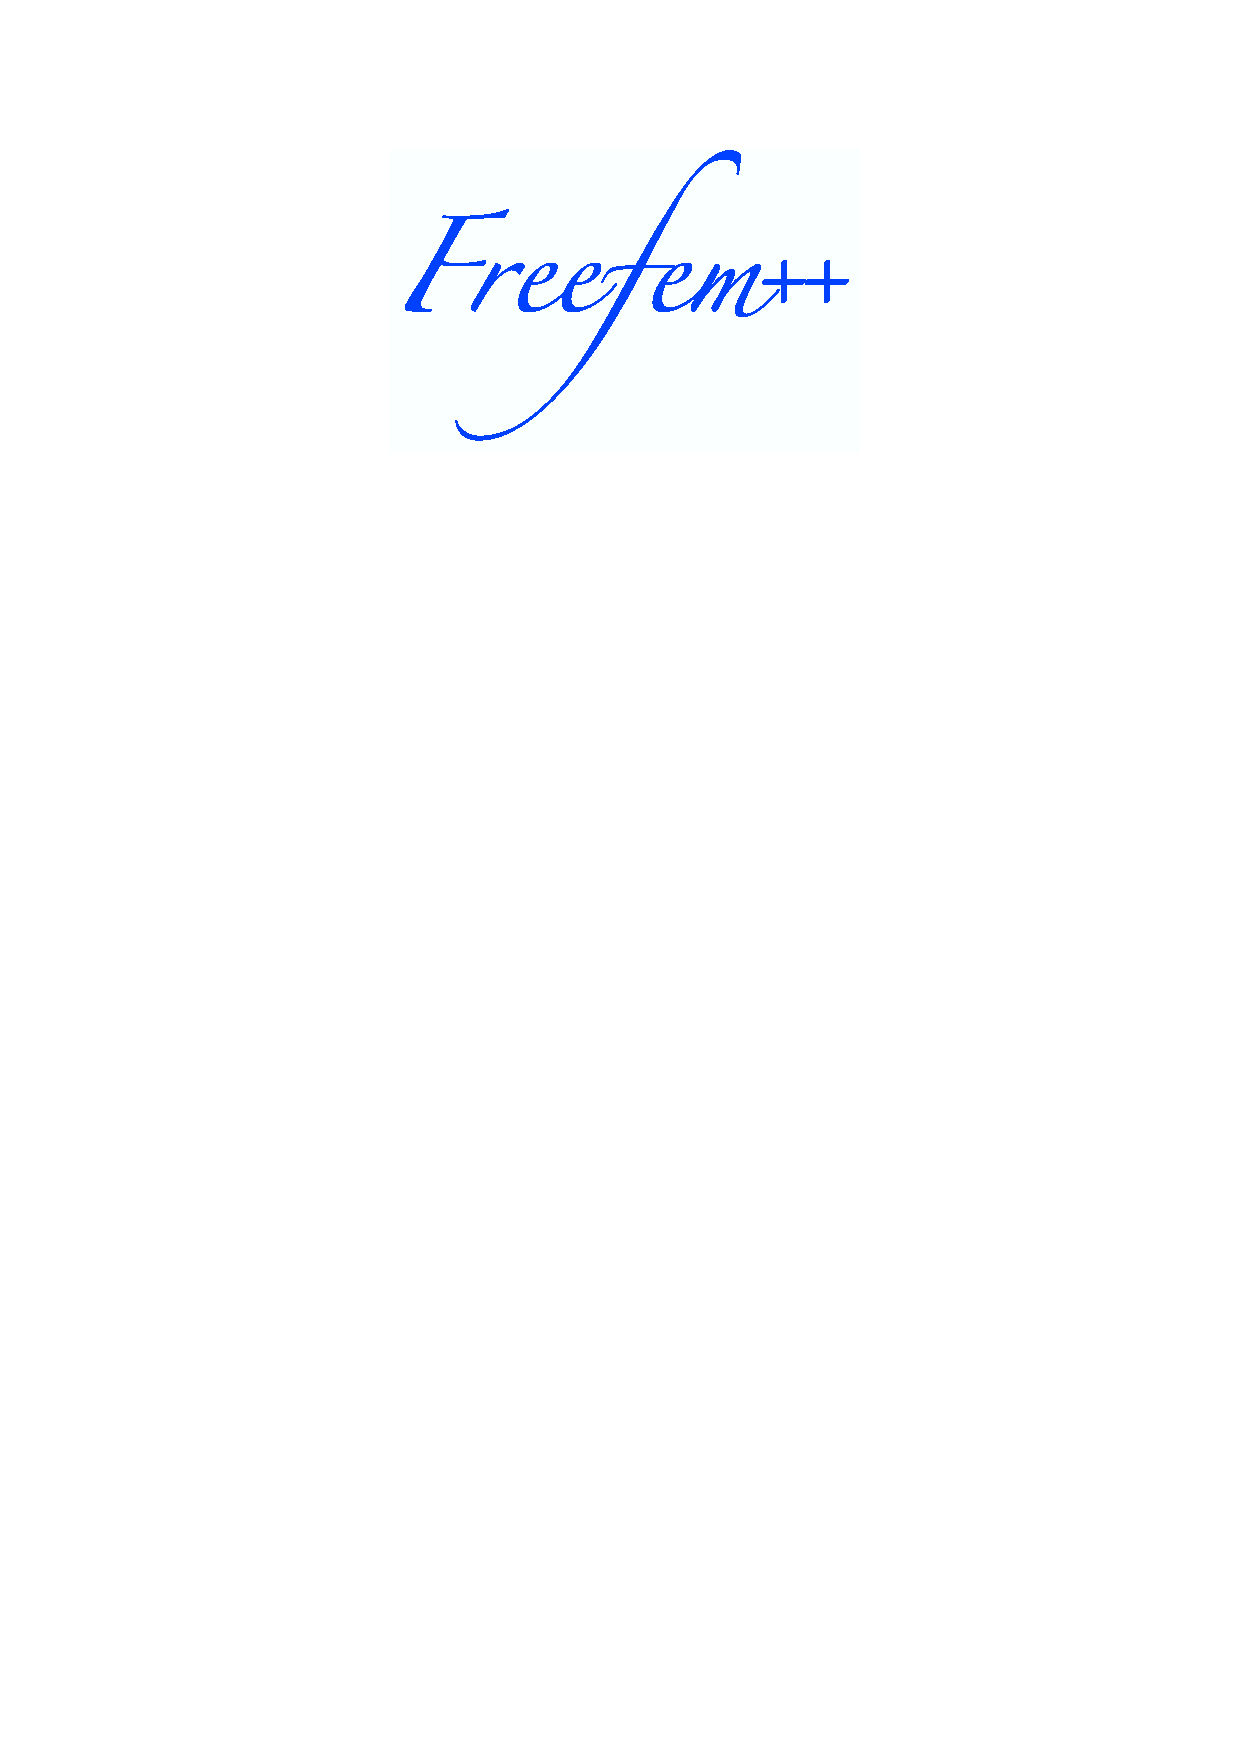
\includegraphics[width=10cm]{titre-ff}
    \\  \large  \Blue{Third Edition,   Version \VERSION }
 \\ \vglue 0.7cm
  {\large \Blue{\url{http://www.freefem.org/ff++}}} \\ ~
 \\~� \\

\includegraphics[width=6cm]{ffauteur}
\vglue 1cm
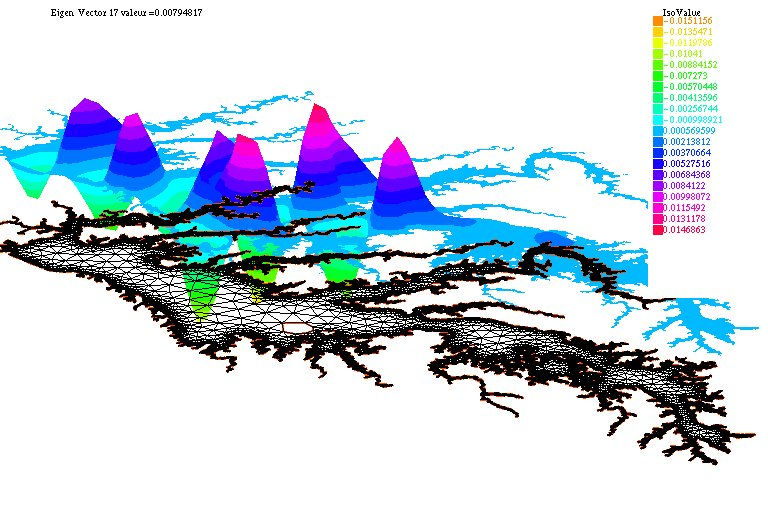
\includegraphics[width=15cm]{chesapeake-2}
\\ \vglue0.5cm
Laboratoire Jacques-Louis Lions, Universit\'{e} Pierre et Marie Curie, Paris
\vglue-2cm
\end{center}}
\clearpage\thispagestyle{empty}\cleardoublepage
\thispagestyle{empty}

\begin{center}
 {\Blue{ \TitreFont FreeFem++}} \\ \vglue 0.0cm  ~ \\
   Third Edition, Version \VERSION
 \\ \vglue 0.7cm
 {\Large \url{http://www.freefem.org/ff++}} \\
\vglue 0.5cm

 \
{\Large Fr\'{e}d\'{e}ric Hecht${}^{1,4}$ }

\url{mailto:frederic.hecht@upmc.fr}

\url{http://www.ann.jussieu.fr/~hecht}


\bigskip

In collaboration with:
\begin{itemize}
\item {\large Sylvian Auliac}, \url{mailto:auliac@ann.jussieu.fr},~\url{http://www.ann.jussieu.fr/auliac}
{is PHD student , he do all the new optimization interface with nlopt, ipopt, cmaes, ...}

\item {\large Olivier Pironneau}, \url{mailto:olivier.pironneau@upmc.fr},~\url{http://www.ann.jussieu.fr/pironneau}
{Olivier Pironneau is a professor of numerical analysis at the university of Paris VI and at LJLL.  His scientific contributions are in numerical methods for fluids.  He is a member of the Institut Universitaire de France and of the French  Academy of Sciences}

\item {\large Jacques Morice}, \url{mailto:morice@ann.jussieu.fr}.
Jacaues Morice is a Post-Doct at LJLL. His doing is Thesis in University of Bordeaux I on fast multipole method (FMM).
In this version, he do all three dimensions mesh generation and coupling with medit software.

\item {\large Antoine Le Hyaric}, \url{mailto:lehyaric@ann.jussieu.fr},~\url{http://www.ann.jussieu.fr/~lehyaric/}
{Antoine Le Hyaric}{ is a research engineer  from the "Centre National de la
Recherche Scientifique" (CNRS) at LJLL . He is an expert in software engineering
for scientific applications. He has applied his skills mainly to
electromagnetics simulation, parallel computing and three-dimensional
visualization.}

\item {\large Kohji Ohtsuka},\url{mailto:ohtsuka@hkg.ac.jp},~ \url{http://www.comfos.org/}
{Kohji Ohtsuka}{ is a professor at the Hiroshima Kokusai Gakuin University, Japan and chairman of the World Scientific and Engineering academy and Society, Japan chapter.  His research is in fracture dynamics, modeling and computing.}
\end{itemize}
\end{center}
\vfill
\hbox to \hsize
{\hss

\includegraphics[height=1.7cm]{LogoLJLL} \hss

\includegraphics[height=1.7cm]{LogoUPMC} \hss
%
\includegraphics[height=1.7cm]{LogoCNRS} \hss

\includegraphics[height=1.7cm]{logo-finance-par-anr} \hss
}
\bigskip

{\small {\bf Acknowledgments}
We are very grateful  to  l'\'Ecole Polytechnique  (Palaiseau, France)  for  printing the second edition of this manual (\url{http://www.polytechnique.fr} ),
and to l'Agence Nationale de la Recherche (Paris, France)
 for funding of the extension  of\ \freefempp to a parallel tridimensional version (\url{http://www.agence-nationale-recherche.fr}) R\'{e}f\'{e}rence : ANR-07-CIS7-002-01.}

\cleardoublepage
%\end{document}
%%%%%%%%%%
 \setcounter{page}{1}
\tableofcontents
\let\subsubsection\subsection
\let\subsection\section
\let\section\chapter
\section*{Preface}

\hbox to \hsize{\hss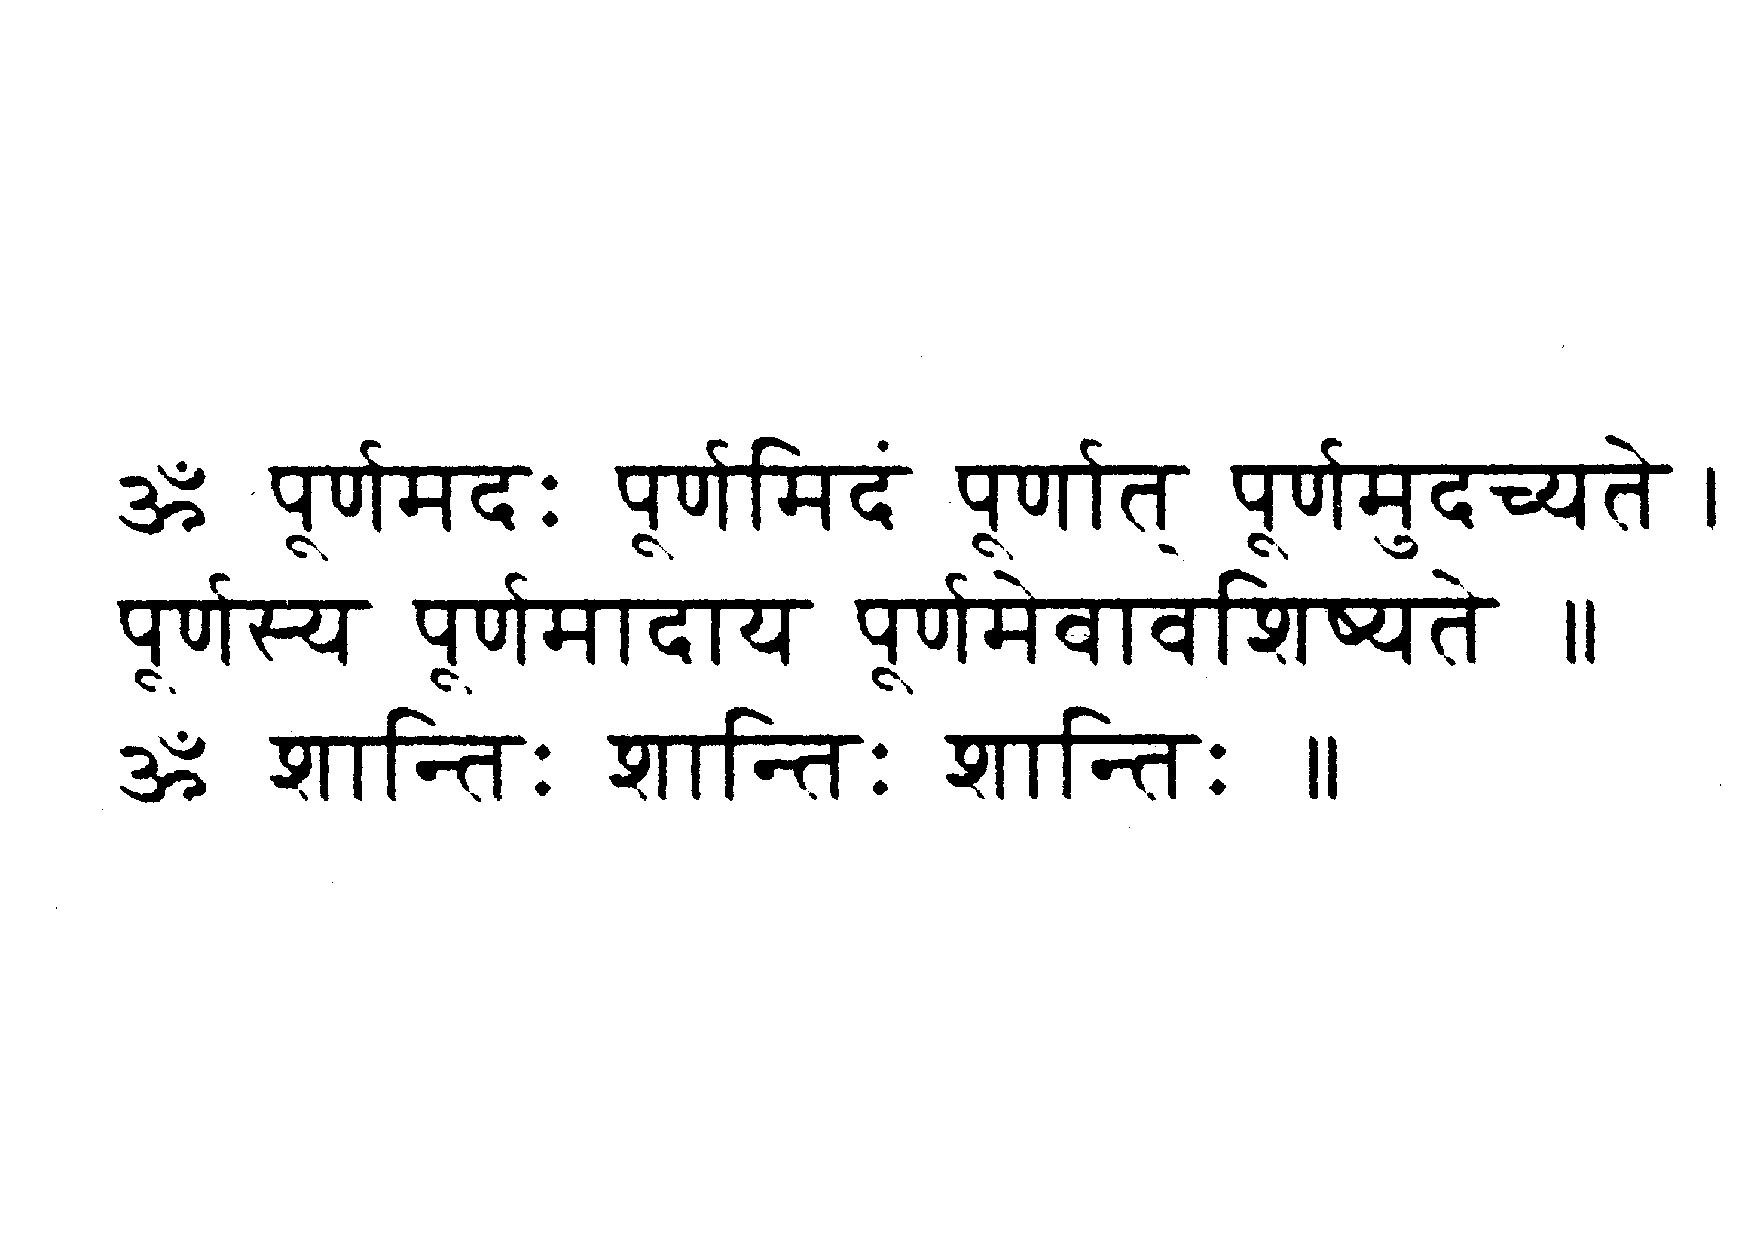
\includegraphics[width=7cm]{sanskrit}}

Fruit of a long maturing process, freefem, in its last avatar, \texttt{FreeFem++}, is a high level integrated development environment (IDE)  for numerically solving partial differential equations (PDE) in dimension 2 and 3.  It is the ideal tool for teaching the finite element method but it is also perfect for research to quickly test new ideas or multi-physics and complex applications.


\medskip

\texttt{FreeFem++} has an advanced automatic mesh generator, capable of a posteriori mesh adaptation; it has a general purpose elliptic solver  interfaced with fast algorithms such as the multi-frontal method UMFPACK, SuperLU . Hyperbolic and parabolic problems are solved by iterative algorithms prescribed by the user with the high level language of \texttt{FreeFem++}. It has several triangular  finite elements, including discontinuous elements.  Finally everything is there in \texttt{FreeFem++} to prepare research quality reports: color display online with zooming and other features and postscript printouts.
\medskip

This manual is meant for students at Master level, for  researchers at any level, and for engineers (including financial engineering) with some understanding of variational methods for partial differential equations.

\section{Introduction}\pagenumbering{arabic} \setcounter{page}{1}
A partial differential equation is a relation between a function
of several variables and its (partial) derivatives.
 Many problems in physics, engineering, mathematics and even banking
are modeled by one or several partial differential equations.
\\\\
\freefempp is a software to solve these equations numerically. As
its name implies, it is a free software (see the copyrights for full detail)
based  on the Finite Element Method; it is not a package, it is an integrated product with its own
high level programming language. This software runs on all UNIX
OS (with g++ 3.3 or later, and OpenGL) , on Window  XP, Vista and 7 and on
MacOS 10 (powerpc, intel) \\\\
Moreover \freefempp is highly adaptive.  Many phenomena involve
several  coupled systems, for example: fluid-structure interactions,
Lorentz forces for aluminium casting and ocean-atmosphere problems are
three such systems. These require different finite element approximations and polynomial
degrees, possibly on different meshes. Some algorithms like
Schwarz' domain decomposition method also require data interpolation
on multiple meshes within one program. \freefempp can handle these
difficulties, i.e. {\it arbitrary finite element spaces on arbitrary
unstructured and adapted bi-dimensional meshes}.  \\\\

The characteristics of \freefempp are:
\begin{itemize}
\item Problem description (real or complex valued) by their variational formulations,
with access to the internal vectors and matrices if needed.
%
\item Multi-variables, multi-equations, bi-dimensional and three-dimensional
 static or time dependent, linear or nonlinear
coupled systems; however the user is required to describe the
iterative procedures which reduce the problem to a set of linear
problems.
%
\item Easy geometric input by analytic description of boundaries by pieces;
however this part is not a CAD system; for instance when two
boundaries intersect, the user must specify the intersection points.
%
\item Automatic mesh generator, based on the Delaunay-Voronoi
algorithm; the inner point density is proportional to the density of
points on the boundaries \cite{George}.
%
\item Metric-based anisotropic mesh adaptation. The metric can be
computed automatically from the Hessian of any \freefempp function
\cite{bamg}.
%
\item High level user friendly typed input language with an algebra
of analytic and finite element functions.
%
\item  Multiple finite element meshes within one application with
automatic interpolation of data on different meshes and possible
storage of the interpolation matrices.
%
\item A large variety of triangular finite elements : linear, quadratic
 Lagrangian elements and more, discontinuous P1 and Raviart-Thomas elements,
 elements of a non-scalar type, the mini-element,\dots{} (but no quadrangles).
%
\index{mean}
\item Tools to define discontinuous Galerkin finite element formulations
\ttCC{P0},\ttCC{P1dc},\ttCC{P2dc} and keywords: \ttCC{jump}, \ttCC{mean}, \ttCC{intalledges}.
%
\item A large variety of linear direct and iterative solvers
(LU, Cholesky, Crout, CG, GMRES, UMFPACK, MUMPS, SuperLU, ...) and eigenvalue and
eigenvector solvers (ARPARK) .
%
\item Near optimal execution speed (compared with compiled C++
implementations programmed directly).

\item Online graphics, generation of \texttt{,.txt,.eps,.gnu, mesh} files
  for further manipulations of input and output data.
%
\item Many examples and tutorials: elliptic, parabolic and hyperbolic problems,
 Navier-Stokes flows, elasticity, Fluid structure interactions,
Schwarz's domain decomposition method, eigenvalue problem, residual
error indicator, ...
%
\item A parallel version using \texttt{mpi}
\end{itemize}

\subsection{Installation }
%%%%%%%%%%%%%%%
\subsubsection{For everyone:}
 First open the following web page
 \begin{center}
  \url{http://www.freefem.org/ff++/}
 \end{center}

And choose your platform: Linux, Windows, MacOS X,
or go to the end of the page to get the full list of downloads.

\begin{remark}: Binaries are available for Microsoft Windows, Apple
Mac OS X and some Linux systems.
%"\texttt{FreeFem++}" at \url{http://www.freefem.org}.
\end{remark}
Install by double click on the appropriate file, under linux and MacOS the
install file are respectively in directory  \texttt{/usr/local/bin},  \texttt{/usr/local/share/freefem++},  \texttt{/usr/local/lib/ff++}


\paragraph{Windows binaries install}

  First download the windows installation executable, then double click it. to install \texttt{FreeFem++}. In most cases just answer yes (or typr return) to all questions. Otherwise in the Additional Task windows, check the  box "Add application directory to your system path your system path ." This is required otherwise the program  \texttt{ffglut.exe} will not be found.

  By now you should have
  two new icons on your desktop:
  \begin{itemize}
   \item \texttt{FreeFem++ (VERSION).exe}  the  \freefempp application.
  % \item \texttt{FreeFem++ (VERSION) GUI.exe}  the GUI \freefempp application, see section \ref{GUI} for more information.
   \item \texttt{FreeFem++ (VERSION) Examples} a link to the \freefempp  folder of  examples.
  \end{itemize}
  where \texttt{(VERSION)} is the version of the files (for example \texttt{3.3-0-P4}).

 By default, the installed files are  in
  \begin{center}
  \verb!C:\Programs Files\FreeFem++!
  \end{center}
  In this directory, you have all the \texttt{.dll} files and
    other applications: \texttt{FreeFem++-nw.exe},\texttt{ffglut.exe}, ...  the \freefempp application
    without graphic windows.
\medskip


The syntax for the command-line tools are the same as those of FreeFem.exe.
%{ \small
%\begin{itemize}
%\item  \verb!FreeFem++.exe [-vnn] [-b] [-s] [-n] [-h] [-f]  [ filepath ]! where the
% \begin{description}
%\item \verb!-b!  no color (black and white plot)
%\item \verb!-n!  no edit
%\item \verb!-s!  not wait at end of execution
%\item \verb!-vnn!  set the level of verbosity to \texttt{nn} before execution of the  script.
%\item  if no file path then you get a dialog box to choose the edp file.
%\end{description}
%\item  \verb!FreeFem++-nw.exe [-v nn]   [[-f] filepath]!
%\end{itemize}}
%\medskip
% where the part in \texttt{[]} is optional.


\paragraph{MacOS X  binaries install}


  Download the MacOS X binary version file, extract all the files with a double click on the
  icon of the file, go the the directory and put the \texttt{FreeFem+.app} application in the
  \texttt{/Applications} directory.
  If you want a terminal access to \freefempp just copy the file \texttt{FreeFem++} in a
   directory of your \verb!$PATH! shell environment variable.

  If you want to automatically launch the \texttt{FreeFem++.app}, double click on a \texttt{.edp} file icon.
  Under the finder pick a \texttt{.edp} in directory \texttt{examples++-tutorial} for example,
  select menu  \texttt{File -> Get Info} an \texttt{change Open with:} (choose FreeFem++.app) and click on button
  \texttt{change All...}.



\paragraph{Where to go from here} An integrated environment called \texttt{FreeFem++-cs}, written by Antoine Le Hyaric,  is provided with \freefempp. Unless you wish to profile now your own development environment, you may proceed to  the next paragraph "How to use FreeFem++".

\subsubsection{For the pros: Installation from sources}

This section is for those who for some reason do not wish to use the binaries and hence need to recompile \freefempp or install it from the source code:

\paragraph{The documentation archive}: The documentation is also open source; to regenerate it you need a \LaTeX{} environment capable of compiling a CVS archive; under MS-Windows you will have to use  \texttt{mingw/msys}
\begin{center}
   \url{http://www.mingw.org}
\end{center}
 and under MacOS X we have used Apple's Developer Tools "Xcode" and  \LaTeX{ } from \url{http://www.ctan.org/system/mac/texmac}.

\paragraph{The C++  archive}:  \freefempp must be compiled  from the source archive, as indicated in \begin{center}
   \url{http://www.freefem.org/ff++/index.htm}
\end{center}
To
extract files from the compressed archive \texttt{freefem++-(VERSION).tar.gz}
to a directory called
\begin{center}
\texttt{freefem++-(VERSION)}
\end{center}
enter the following commands in a shell window~:

\bFF
tar zxvf freefem++-(VERSION).tar.gz
cd freefem++-(VERSION)
\eFF


To compile and install \freefempp, just follow the \texttt{INSTALL}
and \texttt{README} files. The following programs are produced,
depending on the system you are running :
\begin{enumerate}
\item \texttt{FreeFem++}, standard version, with a graphical interface
based on GLUT/OpenGL (use ffglut visualization tool) or not just add \texttt{ -nw } parameter.
\item \texttt{ffglut} the visualization tools  through a pipe of freefem++ (remark: {\it if ffglut is not in the system path,
you will have no plot})
\item \texttt{FreeFem++-nw}, postscript plot output only and  ffmedit (batch version, no graphics windows via \texttt{ffglut} )
\item \texttt{FreeFem++-mpi}, parallel version, postscript output only 
%\item \texttt{FreeFem++-glx}, graphics using OpenGL and X11
%\item \texttt{FreeFem++-cs}, integrated development environment
%\item \texttt{FreeFem++-ag}, integrated development environment
%\item  Sorry, the integrated development environment is reconstruction with the new architecture
% (please see chapter Graphical User Interface \ref{GUI}  for more details).
\item \texttt{/Applications/FreeFem++.app}, the Drag and Drop CoCoa MacOSX
Application
%\item \texttt{FreeFem++-CoCoa}, MacOS Shell script for MacOS OpenGL
%version (MacOS 10.3 or better) (note: it uses
%/Applications/FreeFem++.app)
\item \texttt{bamg} , the bamg mesh generator
\item \texttt{cvmsh2} , a mesh file convertor
\item \texttt{drawbdmesh} , a mesh file viewer
\item \texttt{ffmedit} the freefem++ version of medit software (thanks to P. Frey)
\end{enumerate}

The syntax of tools \texttt{FreeFem++},\texttt{FreeFem++-nw},\texttt{FreeFem++-mpi}, on the command-line  are
{ \small
\begin{itemize}
\item  \verb!FreeFem++ [-?] [-v nn] [-fglut file1] [-glut file2] [-f]  edpfilepath ! where the
\item or \verb!FreeFem++-nw -? [-v nn] [-fglut file1] [-glut file2] [-f]  edpfilepath ! where the
 \begin{description}
 \item \verb!-?!  show the usage.
\item \verb!-fglut filename!  to store all the data for graphic in file \verb! filename!, and to replay do
\verb!ffglut filename!.
\item \verb!-glut  ffglutprogam!  to change the visualisator program's.
\item \verb!-nw! no call to ffglut and medit 
\item \verb!-v nn!  set the level of verbosity to \texttt{nn} before execution of the  script.
\item \verb!-ne! no edp script output
\item \verb!-wait! wait an return in text window before  closing \texttt{FreeFem++}
\item \verb!-nowait! wait an return in text window before  closing \texttt{FreeFem++}
\item \verb!-ne! no edp script output
\item \verb!-cd! Change directory  to script dir (the script path must by global)
\item  if no file path then you get a dialog box to choose the edp file on windows systeme.
\end{description}
\end{itemize}}
\medskip
The notation \texttt{[]} means "optional".


%The FreeFem++ parameter command:
%{\small \begin{verbatim}
%Brochet-2:~ hecht$ FreeFem++
% Syntaxe:
%   FreeFem++ [ -v verbosity ] [ -fglut filepath ] [ -glut command ] [ -nw] [ -f] filename  
%        -v      verbosity : 0 -- 1000000 level of freefem output 
%        -fglut  filepath  : the file name of save all plots (replot with ffglut command ) 
%        -glut    command  : change the command  ffglut 
%        -gff     command  : change the command  ffglut   with  space quotting
%        -nowait           : nowait at the end on text window  ( 
%        -wait             : wait at the end on text window   
%        -nw               : no ffglut and no medit  (=> no graphics windows) 
%        -ne               : no edp script output
%        -cd               : Change directory  to script dir 
% with        default ffglut : ffglut
%\end{verbatim}
%}
\begin{remark} In most cases you can set the level of output (verbosity\index{verbosity}) to value \texttt{nn} by adding the parameters
\texttt{-v nn} on the command line.

\end{remark}

As an installation test, under unix:  go into the directory
\texttt{examples++-tutorial} and run \freefempp on the example script
\texttt{LaplaceP1.edp} with the command~:

\bFF
FreeFem++ LaplaceP1.edp
\eFF

If you are using \texttt{nedit} as your text editor,
do one time \verb!nedit -import edp.nedit! to have coloring syntax for your \ttCC{.edp}
files.


\paragraph{Link with other text editors}
\begin{description}
\item[{notepad++}] at \url{http://notepad-plus.sourceforge.net/uk/site.htm}


\begin{itemize}

\item  Open Notepad++ and Enter  F5
\item   In the new window  enter  the command
\verb!launchff++ "$(FULL_CURRENT_PATH)"!
\item Click on  Save,  and enter  \texttt{FreeFem++} in the box  "Name", now  choose
the  short cut key  to launch directly FreeFem++  (for example \texttt{alt+shift+R})
 \item To add    Color Syntax Compatible with FreeFem++ In Notepad++,
 \begin{itemize}
\item In  Menu \verb!"Parameters"->"Configuration of the  Color Syntax"! proceed as follows:
\item In the list \verb!"Language"! select C++
\item Add "edp" in the  field  \verb!"add ext"!
\item Select  \verb!"INSTRUCTION WORD"! in the  list \verb!"Description"! and in the field
\verb!"supple! \verb!mentary key word"!, cut and past the following list:

\Blue{P0 P1 P2 P3 P4 P5 P1dc P2dc P3dc P4dc P5dc RT0 RT1 RT2 RT3 RT4 RT5 macro plot int1d int2d
solve movemesh adaptmesh trunc checkmovemesh on func buildmesh square Eigenvalue min max
imag exec LinearCG NLCG Newton BFGS LinearGMRES
catch try intalledges jump average mean load savemesh convect abs
sin cos tan atan asin acos cotan sinh cosh tanh cotanh atanh asinh acosh pow
exp log log10 sqrt dx dy endl cout}

\item Select "TYPE WORD" in the list "Description" and ... " "supplementary key word",
cut and past the following list

\Blue{mesh real fespace varf matrix problem string border complex ifstream ofstream}

\item Click on \texttt{Save \& Close}.  Now nodepad++ is configured.
\end{itemize}
\end{itemize}

\item[{Crimson}] {\bf Editor}
availble at \url{http://www.crimsoneditor.com/} and adapted as follows:

\begin{itemize}
\item Go to the \texttt{Tools/Preferences/File} association menu and add the .edp extension set

\item In the same panel in \texttt{Tools/User} Tools, add a \texttt{FreeFem++} item (1st line) with the path
to \texttt{freefem++.exe} on the second line and \texttt{\$(FilePath)} and \texttt{\$(FileDir)} on third and fourth lines.
Tick the 8.3 box.
\item for color syntax, extract file from \texttt{crimson-freefem.zip} and put files in the corresponding sub-folder of
 Crimson folder (\verb.C:\Program Files\Crimson Editor. ).
\end{itemize}

\item[winedt] for Windows : this is the best but it could be tricky to set up.  Download it from
\begin{center}
 \url{http://www.winedt.com}
 \end{center}
 this is a multipurpose text editor  with advanced features
such as syntax coloring; a macro is available on \url{www.freefem.org} to localize winedt to \freefempp
without disturbing the winedt functional mode for LateX, TeX, C, etc.  However winedt is not free
after the trial period.

\item[TeXnicCenter] for Windows: this is the easiest and will be the best once we find a volunteer
to program the color syntax.  Download it from
\begin{center}\url{http://www.texniccenter.org/}\end{center}
It is also an editor for TeX/LaTeX. It has a "`tool"' menu which can be configured to launch
\freefempp programs as in:
\begin{itemize}
\item Select the \texttt{Tools/Customize} item which will bring up a dialog box.
\item Select the  \texttt{Tools} tab and  create a new item: call it \texttt{freefem}.

\item in the 3 lines below,
 \begin{enumerate}
\item  search for \texttt{FreeFem++.exe}
\item select Main file with further option
 then Full path and click also on the \texttt{8.3 box}
 \item select main file full directory path with 8.3
 \end{enumerate}
\end{itemize}
\item[nedit] on the Mac OS, Cygwin/Xfree and linux, to import the color syntax do

\verb!nedit -import edp.nedit!

 \item[Smultron] on the Mac, available at \url{http://smultron.sourceforge.net}. It comes ready with color syntax for .edp file.  To teach it to launch \freefempp files, do a "command B" (i.e. the menu Tools/Handle Command/new command) and create a command which does
 \begin{verbatim}
 /usr/local/bin/FreeFem++-CoCoa %%p
 \end{verbatim}

\end{description}
%
\begin{figure}[htbp]
\begin{center}
\includegraphics[width=15cm]{crimpson}
\caption{ Integrated environment for FreeFem++ development with Windows
   \label{fig:mi}}
\end{center}
\end{figure}


\subsection{How to use \freefempp}

%\paragraph{Under Windows with Graphic Interfaces}

%The executable \texttt{freefem++.exe} opens a dialog box for
%choosing the input file, then it executes the input file content and produces
%graphics and output files.
%\\\\
%You can create and modify \freefempp programs with your favorite text editor.
%\\\\
%An integrated environment (\freefempp GUI), written by A. Le Hyaric, is also included
%with the distribution. the application name is \texttt{FreeFem++-cs}; note however that
%the graphics display is slower in this mode.
%There are other ways to have an integrated environment. TeX users usually have
%an editor installed; if it is winedt or TeXnicCenter then these can
%be programmed to handle the edit-run-correct cycle of \freefempp with
%color syntax and automatic launch of freefem.  If you don't have one of these
%installed the easiest is to download the freeware \texttt{Crimson Editor}.
%\begin{figure}[htbp]
%\begin{center}
%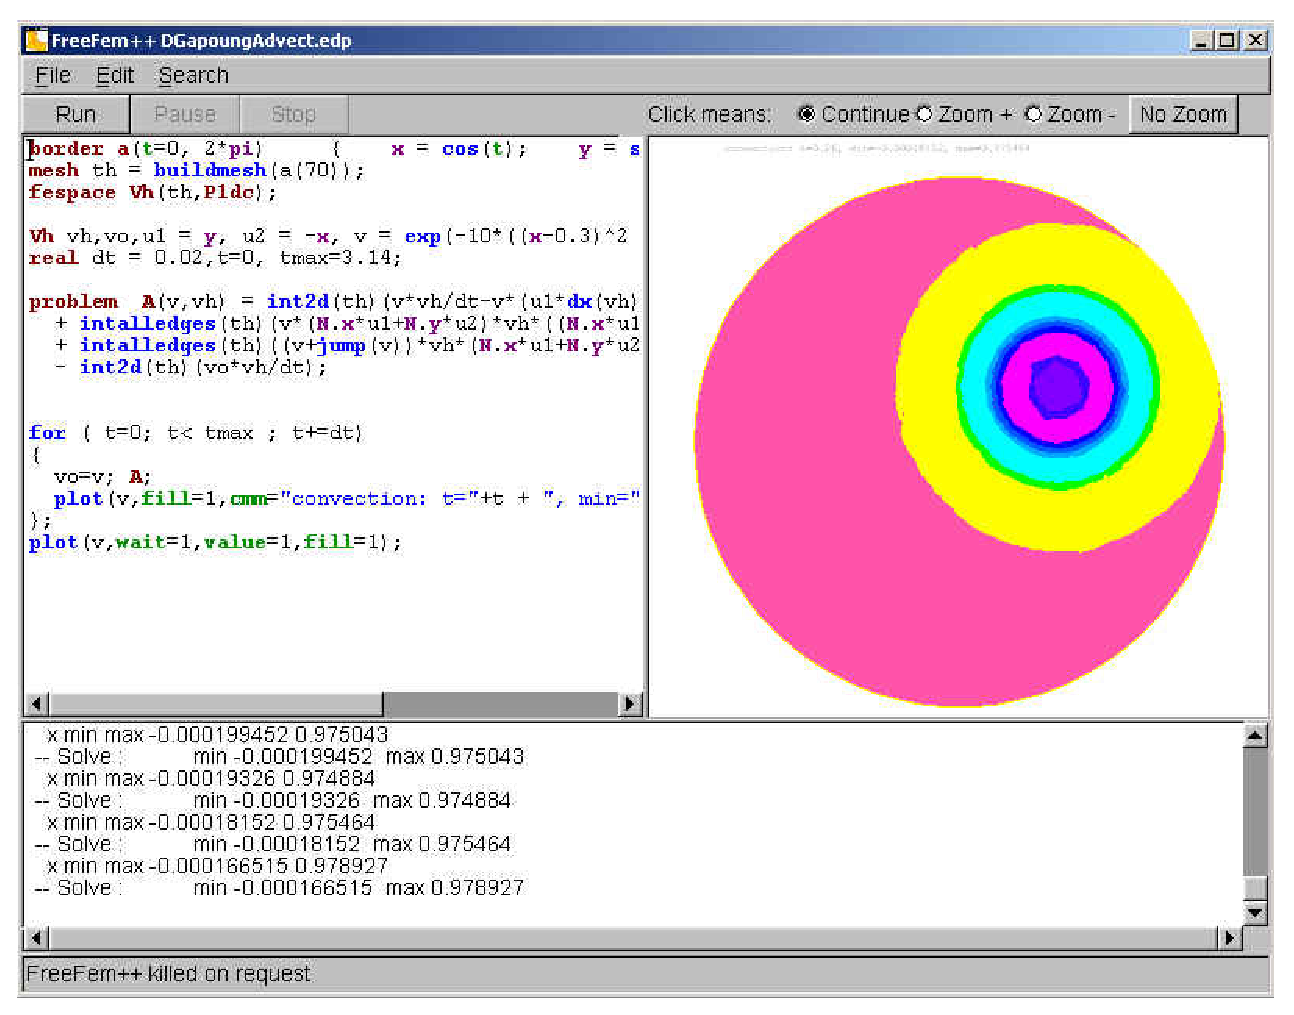
\includegraphics[width=15cm]{csSnapOld}
%\caption{ The 3 panels of the integrated environment \texttt{freefem++-cs}:
%to the top left one has the program (which can be edited?), on the top right the graphic output window, and the bottom pane displays text messages.
%}
%\end{center}
%\end{figure}
\paragraph{Under MacOS X with Graphic Interfaces}

To test  an \texttt{.edp} file, just drag and drop
the file icon  on the MacOS application icon  \texttt{FreeFem++.app}.
You can also launch this application and use the menu:  $\mathtt{File} \rightarrow \mathtt{Open}$.

One of the best ways however on the Mac is to use a text editor like \texttt{Smultron.app}
(see above).
\begin{figure}[htbp] %  figure placement: here, top, bottom, or page
   \centering
   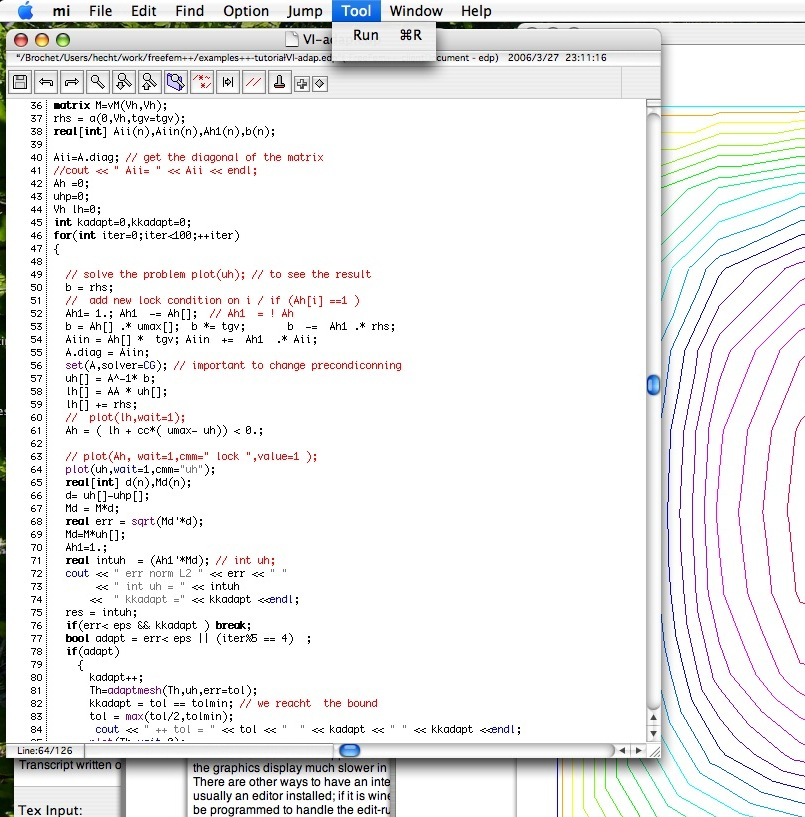
\includegraphics[width=10cm]{mi.jpg}
   \caption{The 3 panels of the integrated environment built with the
\texttt{fraise Editor} with \freefempp in action. The Tools menu
has an item to launch \freefempp by a Ctrl+1 command.}
\end{figure}

\paragraph{In Terminal mode}

Choose the type of application from \texttt{FreeFem++}, \texttt{FreeFem++-nw},  \texttt{FreeFem++-mpi}, \dots  according to your needs.  Add at least the path name; for example
\bFF
 FreeFem++ your-edp-file-path
\eFF

\subsection{Environment variables, and the init file}


\index{verbosity}\index{includepath}\index{loadpath}\index{load}\index{include}
 \texttt{FreeFem++} reads a user's init file named \ttCC{freefem++.pref}
 to initialize global variables:
   \texttt{verbosity}, \texttt{includepath}, \texttt{loadpath}.

\begin{remark} The variable \texttt{verbosity} changes the level of internal printing ($0$, nothing (unless there are syntax errors), $1$ few,  $10$  lots, etc. ...),
the default value is $2$.
\\
 The include files are searched from the \texttt{includepath} list and the load files
are searched from  \texttt{loadpath} list.
\end{remark}

 The syntax of the file  is:
\begin{verbatim}
     verbosity= 5
     loadpath += "/Library/FreeFem++/lib"
     loadpath += "/Users/hecht/Library/FreeFem++/lib"
     includepath  += "/Library/FreeFem++/edp"
     includepath  += "/Users/hecht/Library/FreeFem++/edp"
     #  comment
     load += "funcTemplate"
     load += "myfunction"
     load += "MUMPS_seq" 
\end{verbatim}

 The possible paths for this file  are
 \begin{itemize}
   \item under unix and MacOs
\begin{verbatim}
	 /etc/freefem++.pref
    $(HOME)/.freefem++.pref
    freefem++.pref
\end{verbatim}
  \item under windows
\begin{verbatim}
     freefem++.pref
\end{verbatim}
\end{itemize}

We can also use shell environment variable to change verbosity and
the search rule before the init files.

\begin{verbatim}
    export FF_VERBOSITY=50
    export FF_INCLUDEPATH="dir;;dir2"
    export FF_LOADPATH="dir;;dir3""
\end{verbatim}

 Remark: the separator between directories must be ";" and not ":" because ":" is used under Windows.

 Remark, to show the list of init of \texttt{freefem++}, do
\begin{verbatim}
 export FF_VERBOSITY=100; ./FreeFem++-nw
 --  verbosity is set to 100
 insert init-files /etc/freefem++.pref $
...
\end{verbatim}

\subsection{History}

The project has evolved from \texttt{MacFem, PCfem}, written in
Pascal. The first C version lead to \texttt{freefem 3.4}; it offered
mesh adaptativity on a single mesh only.
\\\\
A thorough rewriting in C++ led to \texttt{freefem+}
(\texttt{freefem+ 1.2.10} was its last release), which included
interpolation over multiple meshes (functions defined on one mesh
can be used on any other mesh); this software is no longer
maintained but still in use because it handles a problem description
using the strong form of the PDEs. Implementing the interpolation
from one unstructured mesh to another was not easy because it had to
be fast and non-diffusive; for each point, one had to find the
containing triangle. This is one of the basic problems of
computational geometry (see Preparata \& Shamos\cite{Preparata} for
example). Doing it in a minimum number of operations was the
challenge. Our implementation is $O(n\log n)$ and based on a
quadtree.  This version also grew out of hand because of the
evolution of the template syntax in C++.
 \\\\
We have been working for a few years now on \freefempp, entirely
re-written again in C++ with a thorough usage of {\tt template} and
generic programming
for coupled systems of unknown size at compile time. Like all
versions of \texttt{freefem} it has a high level user friendly input
language which is not too far from the mathematical writing of the
problems.
\\\\

The freefem language allows for a quick specification of any partial
differential system of equations.  The language syntax of \freefempp
is the result of a new design which makes use of the STL \cite{cpp},
templates and \texttt{bison} for its implementation; more detail can
be found in \cite{FHcpp}.
  The outcome is a
versatile software in which any new finite element can be included
in a few hours; but a recompilation is then necessary.  Therefore
the library of finite elements available in \freefempp will grow
with the version number and with the number of users who program
more new elements. So far we have discontinuous $P_0$
elements,linear $P_1$ and quadratic $P_2$ Lagrangian elements,
discontinuous $P_1$ and Raviart-Thomas elements and a few others like bubble elements.


\section{Getting Started}
\label{sec:example}

To illustrate with an example,
let us explain how \freefempp solves
\textbf{Poisson}'s equation: \emph{for a given function $f(x,y)$, find a
function $u(x,y)$ satisfying}
\begin{eqnarray}
\label{eqn:Poisson}
-\Delta u(x,y) &=& f(x,y)\quad \mbox{ for all }(x,y)\in\Omega,
 \\ \label{eqn:Dirichlet}
  u(x,y) &=& 0\quad \mbox{ for all }(x,y)\mbox{ on }\p\Omega,.
\end{eqnarray}
Here $\partial\Omega$ is the boundary of the bounded open set $\Omega\subset \R^2$
and  $ \Delta u = \frac{\p^2 u}{\p x^2 } + \frac{\p^2 u}{\p y^2}$.


The following is a \freefempp program which computes $u$ when
$f(x,y)=xy$  and $\Omega$ is the unit disk. The boundary
$C=\p\Omega$ is
$$
C=\{(x,y)|\; x=\cos(t),\, y=\sin(t),\, 0\le t\le 2\pi\}
$$

Note that in \freefempp the domain $\Omega$ is assumed to described by its boundary
that is on the left side of its boundary oriented by the parameter.
%
%By definition the domain is on the left side of the boundary
%oriented by the parameter $t$.
 As illustrated in Fig. \ref{firstU},
we can see the isovalue of $u$ by using \ttCC{@plot} (see line 13
below).
\twoplot[height=5cm]{firstTh}{firstU}{mesh \texttt{Th} by \texttt{build(C(50))}}{isovalue by \texttt{plot(u)}}


\index{clock}
\begin{example}\label{exm:first}~
\bFF
    // defining the boundary \hfilll
 1: @border C(t=0,2*@pi){@x=cos(t); @y=sin(t);}
    // the triangulated domain Th is on the left side of its boundary \hfilll
 2: @mesh Th = @buildmesh (C(50));
    // the finite element space defined over Th is called here Vh
 3; @fespace Vh(Th,@P1);
 4: Vh u,v;  // defines u and v as piecewise-P1 continuous functions
 5: @func f= x*y;  // definition of a called f function
 6: @real cpu=clock(); // get the clock in second
 7: @solve Poisson(u,v,@solver=LU) =  // defines the PDE
 8:    @int2d(Th)(@dx(u)*@dx(v) + @dy(u)*@dy(v))   //  bilinear part
 9:    - @int2d(Th)( f*v)          // right hand side
 10:    + @on(C,u=0)  ;  // Dirichlet boundary condition
 11: @plot(u);
 12: @cout << " CPU time = " << clock()-cpu << @endl;
\eFF
\end{example}
Note that the qualifier \texttt{solver=LU} is not required and by default a
multi-frontal LU would have been used. Note also that the lines
containing \texttt{clock} are equally not required. Finally note how
close to the mathematics \freefempp input language is. Line \texttt{8} and  \texttt{9}
correspond to the mathematical variational equation
\[
    \int_{T_h}(\frac{\p u}{\p x}\frac{\p v}{\p x}
    +\frac{\p u}{\p y}\frac{\p v}{\p
    y})\d x \d y
    =
   \int_{T_h}f v\d x\d y
\]
for all $v$ which are in the finite element space $V_h$ and zero on
the boundary $C$.
\paragraph{Exercise}:
Change P1 into P2 and run the program.


\subsubsection{FEM by \freefempp: how does it work?}
This first example shows how \freefempp executes  with no effort all
the usual steps required by the finite element method (FEM). Let us
go through them one by one.
\\\\
\textbf{1st line:} the boundary $\Gamma$ is described analytically
by a parametric equation for $x$ and for $y$. When
$\Gamma=\sum_{j=0}^J \Gamma_j$ then each curve $\Gamma_j$, must be
specified and crossings of $\Gamma_j$ are not allowed except at end
points .

The keyword ``label'' can be added to define a group
of boundaries for later use (boundary conditions for instance).
 Hence the circle could also have been described as two half circle with
 the same label:
 \bFF
@border Gamma1(t=0,@pi)   {@x=cos(t); @y=sin(t); @label=C}
@border Gamma2(t=@pi,2*@pi){@x=cos(t); @y=sin(t); @label=C}
 \eFF
Boundaries can be referred to  either by name (\ttCC{Gamma1} for example) or by label (\ttCC{C} here)
or even by its internal number here 1 for the first half circle and 2 for the second
(more examples are in \refSec{Meshing Examples}).
\\\\
\textbf{2nd line:} the triangulation $\mathcal{T}_h$ of $\Omega$ is
automatically generated  by \ttCC{@buildmesh(C(50))} using $50$
points on \ttCC{C} as in Fig. \ref{firstTh}.

The domain is assumed to be on the left side of the boundary which is implicitly
oriented by the parametrization. So an elliptic hole can be added by
 \bFF
 @border C(t=2*@pi,0){@x=0.1+0.3*cos(t); @y=0.5*sin(t);}
 \eFF
If by mistake one had written
 \bFF
 @border C(t=0,2*@pi){@x=0.1+0.3*cos(t); @y=0.5*sin(t);}
 \eFF
then the inside of the ellipse would be triangulated as well as the outside.

Automatic mesh generation is
based on the Delaunay-Voronoi algorithm. Refinement of the mesh are
done by increasing the number of points on $\Gamma$, for example,
\ttCC{@buildmesh(C(100))}, because inner vertices are determined
by the density of points on the boundary. Mesh adaptation can be performed also
against a given function \ttCC{f} by calling \ttCC{@adaptmesh(Th,f)}.

Now the name $\mathcal{T}_h$ (\texttt{Th} in \freefempp) refers to
the family $\{T_k\}_{k=1,\cdots,n_t}$ of triangles shown in figure \ref{firstTh}.
Traditionally  $h$ refers to the mesh size, $n_t$ to the number of
triangles in $\mathcal{T}_h$ and $n_v$ to the number of vertices, but it is seldom
that we will have to use them explicitly.
If $\Omega$ is not a polygonal domain, a ``skin'' remains between
the exact domain $\Omega$ and its approximation
$\Omega_h=\cup_{k=1}^{n_t}T_k$.
However, we notice that all corners of $\Gamma_h = \p\Omega_h$ are
on $\Gamma$.
\\\\
\textbf{3rd line:} A finite element space is, usually, a space of
polynomial functions on elements, triangles here only, with certain matching properties
at edges, vertices etc.  Here \ttCC{@fespace Vh(Th,P1)} defines $V_h$ to be the
space of continuous functions which are affine in $x,y$ on each triangle of $T_h$.  As it is a
linear vector space of finite dimension, basis can be found.
The canonical basis is made of functions, called the \index{hat function}\emph{hat functions}
$\phi_k$ which are continuous piecewise affine and are equal to 1 on one vertex and 0 on all others.
A typical hat function is shown on figure \ref{fig-hatFunction}
\footnote{
The easiest way to define $\phi_k$ is by making use of the \index{barycentric coordinates}
\emph{barycentric coordinates}
$\lambda_i(x,y),~i=1,2,3$ of a point $q=(x,y)\in T$, defined by
\[
    \sum_i\lambda_i=1,~~~\sum_i\lambda_i\vec q^i=\vec q
\]
where $q^i,~i=1,2,3$ are the 3 vertices of $T$.  Then it is easy to see that
the restriction of $\phi_k$ on $T$ is precisely $\lambda_k$.
}.
Then
\begin{equation}
V_h(\mathcal{T}_h,P_1)=\left\{w(x,y)\left|\;
w(x,y)=\sum_{k=1}^{M}w_k\phi_k(x,y),\, w_k\textrm{ are real numbers}\right.\right\}
\label{eq 2.3}\end{equation}
where $M$ is the dimension of $V_h$, i.e. the number of vertices.
The $w_k$ are called the \index{degree of freedom}\emph{degree of freedom} of $w$ and $M$ the number of
the degree of freedom.

\begin{figure}[htbp]
\begin{minipage}{\textwidth}
\begin{minipage}{0.3\textwidth}
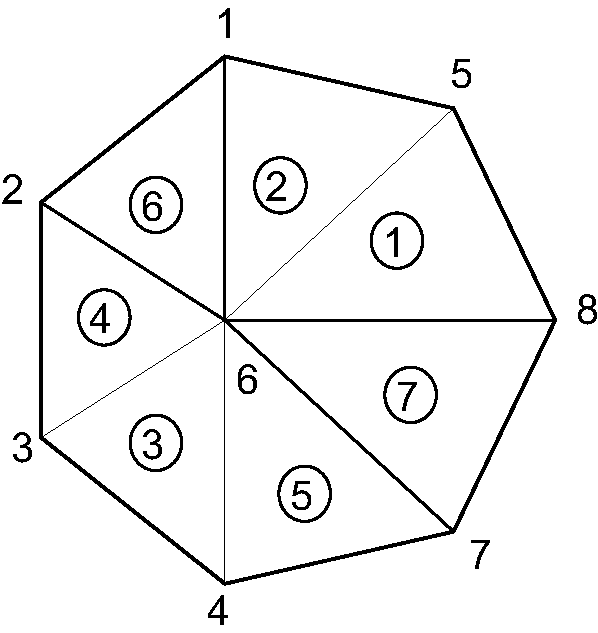
\includegraphics[width=\textwidth]{secondT}%
\caption{mesh \texttt{Th}}
\end{minipage}
\hspace{0.5mm}
\begin{minipage}{0.7\textwidth}
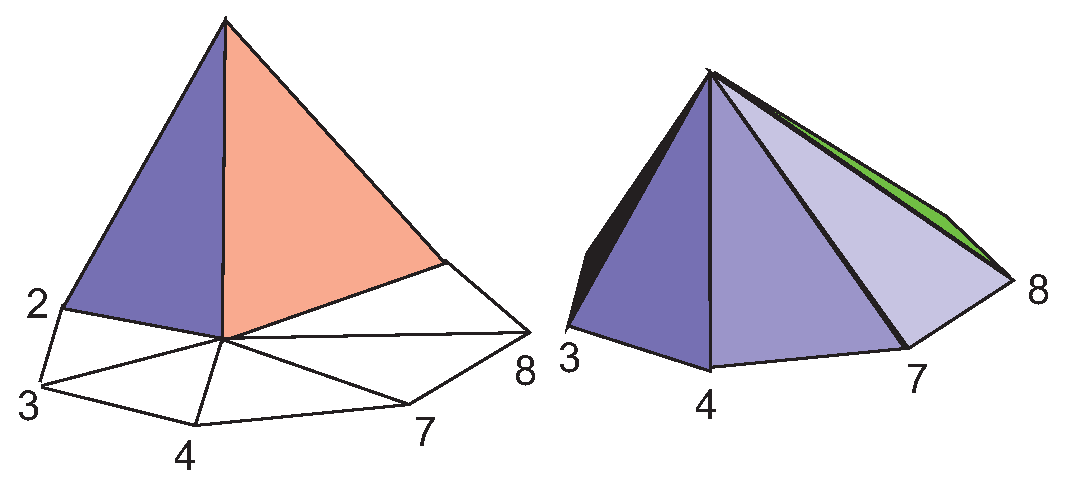
\includegraphics[width=\textwidth]{hat}%
\caption{Graph of $\phi_1$ (left) and $\phi_6$ \label{fig-hatFunction}}
\end{minipage}
\end{minipage}
\end{figure}
It is said also that the \index{nodes}\emph{nodes} of this finite element method
are the vertices.
\\
\index{fespace!P0}
\index{fespace!P1}
\index{fespace!P2}
\index{fespace!RT0}
\index{fespace!P1nc}
\index{fespace!P1dc}
\index{fespace!P2dc}
\index{fespace!P1b}
\index{fespace!P2b}
\index{fespace!P3}\index{fespace!P4}\index{fespace!RT1}\index{fespace!BDM1}\index{fespace!Morley}\index{fespace!P3dc}\index{fespace!P4dc}\index{fespace!RT0Ortho}\index{fespace!RT1Ortho}\index{fespace!BDM1Ortho}\index{fespace!P2BR}\index{fespace!P2h}
Currently \freefempp implements the following elements \index{elements} in 2d, (see section \ref{finite elements} for the full description)
{\parskip=0cm
\par \ttCC{P0} piecewise constant,
\par \ttCC{P1} continuous piecewise linear,
\par \ttCC{P2} continuous piecewise quadratic,
\par \ttCC{P3} continuous piecewise cubic, (need  \ttCC{@load "Element_P3"})
\par \ttCC{P4} continuous piecewise quartic,(need  \ttCC{@load "Element_P4"})
\par \ttCC{RT0} Raviart-Thomas piecewise constant,
\par \ttCC{RT1} Raviart-Thomas degree 1  piecewise constant (need  \ttCC{@load "Element_Mixte"})
\par \ttCC{BDM1} Brezzi-Douglas-Marini degree 1  piecewise constant (need  \ttCC{@load "Element_Mixte"})
\par \ttCC{RT0Ortho} Nedelec type 1 degree 0  piecewise constant 
\par \ttCC{RT1Ortho} Nedelec type 1 degree 1  piecewise constant (need  \ttCC{@load "Element_Mixte"})
\par \ttCC{BDM1Ortho} Brezzi-Douglas-Marini degree 1  piecewise constant (need  \ttCC{@load "Element_Mixte"})
\par \ttCC{P1nc} piecewise linear non-conforming,
\par \ttCC{P1dc} piecewise linear discontinuous,
\par \ttCC{P2dc} piecewise quadratic discontinuous,
\par \ttCC{P2h}  quadratic homogene continuous (without P1)
\par \ttCC{P3dc} piecewise cubic discontinuous,(need  \ttCC{@load "Element_P3dc"})
\par \ttCC{P4dc} piecewise quartic discontinuous,(need  \ttCC{@load "Element_P4dc"})
\par \ttCC{P1b} piecewise linear continuous plus bubble,
\par \ttCC{P2b} piecewise quadratic continuous plus bubble.
\par \ttCC{Morley} Morley finite element (need   \ttCC{@load "Morley"})
\par \ttCC{P2BR} P2 Bernardi-Raugel finite element  (need   \ttCC{@load "BernadiRaugel.cpp"})

\par \ttCC{P0edge} a finite element constant per edge 
\par \ttCC{P1edge} to \ttCC{P5edge}  a finite element polynomial  on edge (need   \ttCC{@load "Element_PkEdge"})

\par {...} \par
}

\index{fespace!P03d}
\index{fespace!P13d}
\index{fespace!P23d}
\index{fespace!RT03d}
\index{fespace!Edge03d}
\index{fespace!P1b3d}
Currently \freefempp implements the following elements \index{elements} in 3d, (see section \ref{finite elements} for the full description)
{\parskip=0cm
\par \ttCC{P03d} piecewise constant,
\par \ttCC{P13d} continuous piecewise linear,
\par \ttCC{P23d} continuous piecewise quadratic,
\par \ttCC{RT03d} Raviart-Thomas piecewise constant,
\par \ttCC{Edge03d} The Nedelec Edge element
\par \ttCC{P1b3d} piecewise linear continuous plus bubble,
\par {...} \par
}
To get the full list, in a unix terminal, in directory \texttt{examples++-tutorial} do
\bFF
FreeFem++ dumptable.edp
grep TypeOfFE lestables
\eFF

Note that other elements can be added fairly easily.
\\\\
\textbf{Step3: Setting the problem}
\\
\textbf{4th line:} \texttt{Vh u,v} declares that $u$ and $v$ are approximated as above,
namely
\begin{equation}\label{defu}
u(x,y)\simeq u_h(x,y)=\sum_{k=0}^{M-1} u_k\phi_k(x,y)
\end{equation}
\textbf{5th line:} the right hand side \ttCC{f} is defined analytically using the keyword
\ttCC{@func}.

\textbf{7th--9th lines:} defines the bilinear form of equation (\ref{eqn:Poisson}) and
its Dirichlet boundary conditions (\ref{eqn:Dirichlet}).
\\
This \emph{variational formulation} is derived by
multiplying (\ref{eqn:Poisson}) by $v(x,y)$ and integrating
the result over $\Omega$:
$$
-\int_{\Omega}v\Delta u \,\d x\d y = \int_{\Omega} vf\, \d x\d y
$$
Then, by Green's formula, the problem  is converted into finding $u$
such that
\begin{eqnarray}
\label{eqn:weakform}
&&a(u,v) - \ell(f,v) = 0
\qquad \forall v \hbox{ satisfying $v=0$ on }\p\Omega.\\
&&\hbox{with }a(u,v)=\int_{\Omega}\nabla u\cdot \nabla v \,\d x\d y ,
\quad \ell(f,v)=\int_{\Omega}fv\, \d x\d y
\label{eqn:bilinear}
\end{eqnarray}
 In \freefempp
the \textbf{Poisson} problem can be  declared only as in
\bFF
  Vh u,v; @problem Poisson(u,v) =
\eFF
and solved later as in
\bFF
...
  Poisson; //   the problem is solved here
...
\eFF
or declared and solved at the same time as in
\begin{center}
\ttCC{Vh u,v; @solve Poisson(u,v) =@int(...}
\end{center}
and (\ref{eqn:weakform}) is written with \ttCC{@dx}(u) $=\p
u/\p x$, \ttCC{@dy}(u) $=\p u/\p y$ and
\begin{eqnarray*}
&&\int_{\Omega}\nabla u\cdot \nabla v\, \d x\d y \longrightarrow
\ttCC{@int2d(Th)( @dx(u)*@dx(v) + @dy(u)*@dy(v) )}\\
&&\int_{\Omega}fv\, \d x\d y \longrightarrow
\ttCC{@int@2d(Th)( f*v )}\qquad
\textrm{(Notice here, $u$ is unused)}\\
\end{eqnarray*}
In \freefempp {\bf bilinear terms and linear terms should not be under the same integral}; indeed to construct the linear systems
 \freefempp finds out which integral contributes to the bilinear form by checking if both terms , the unknown (here \texttt{u}) and test functions (here \texttt{v}) are present.
 \\\\
\textbf{Step4: Solution and visualization}\\

\textbf{6th line:} The current time in seconds is stored into the real-valued variable \ttCC{cpu}.

\textbf{7th line} The problem is solved.

\textbf{11th line:} The visualization is done as illustrated in Fig. \ref{firstU}
(see \refSec{Plot} for zoom, postscript and other commands).

\textbf{12th line:} The computing time (not counting graphics) is written on the console
Notice the C++-like syntax; the user needs not study C++ for using \freefempp,
but it helps to guess what is allowed in the language.
\\\\
\textbf{Access to matrices and vectors}
\\
Internally \freefempp will solve a linear system of the type
\begin{eqnarray}
\label{eqn:Equation}
\sum_{j=0}^{M-1} A_{ij}u_j - F_i=0 ,\quad i=0,\cdots,M-1;\qquad
F_i=\int_{\Omega}f\phi_i\, \d x\d y
\end{eqnarray}
which is found by using (\ref{defu}) and replacing $v$ by $\phi_i$
in (\ref{eqn:weakform}).
And the Dirichlet conditions are implemented by penalty,
namely by setting $A_{ii}=10^{30}$  and
 $F_i=  10^{30}*0$ if $i$ is a boundary degree of freedom. Note, that the number $10^{30}$ is called \ttCC{tgv}
 (\emph{tr\`es grande valeur})
 and it is generally possible to change this value \index{solve!tgv=}, see the index item \texttt{solve!tgv=}.

\medskip\index{matrix}\index{varf}

The matrix $A=(A_{ij})$ is called \emph{stiffness matrix} \index{matrix!stiffness matrix}.


If the user wants to access $A$ directly he can do so
by using (see section \ref{matrix-varf} page \pageref{matrix-varf} for details)
\bFF
@varf a(u,v) = @int2d(Th)( @dx(u)*@dx(v) + @dy(u)*@dy(v))
               + @on(C,u=0) ;
@matrix A=a(Vh,Vh);  // stiffness matrix,
\eFF

The vector $F$ \index{[]@\verb=[]=}
in (\ref{eqn:Equation}) can also be constructed manually
\bFF
@varf l(unused,v) = @int2d(Th)(f*v)+@on(C,unused=0);
Vh F;  F[] = l(0,Vh); //  F[] is the vector associated to the function \texttt{F}
\eFF
The problem can then be solved by
\bFF
 u[]=A^-1*F[]; // u[] is the vector associated to the function u
\eFF
\begin{note}
  Here \ttCC{u} and \ttCC{F} are finite element function, and  \ttCC{u[]} and
  \ttCC{F[]} give  the array of value associated ( \ttCC{u[]}$\equiv (u_i)_{i=0,\dots,M-1}$ and
  \ttCC{F[]}$\equiv (F_i)_{i=0,\dots,M-1}$). So we have
   $$
   \mathtt{u}(x,y) = \sum_{i=0}^{M-1} \mathtt{u[][}i\mathtt{]} \phi_i(x,y) ,
   \qquad \mathtt{F}(x,y) = \sum_{i=0}^{M-1} \mathtt{F[][}i\mathtt{]} \phi_i(x,y)
   $$
   where $\phi_i, i=0...,,M-1$ are the basis functions of  \texttt{Vh} like in equation
   (\ref{eq 2.3}), and $M = \mathtt{Vh.ndof}$ is  the number of degree of freedom (i.e. the dimension of the space \texttt{Vh}).

\end{note}
The linear system (\ref{eqn:Equation}) is solved by \texttt{UMFPACK}
unless another option is mentioned specifically  as in
\begin{center}
\ttCC{Vh u,v; @problem Poisson(u,v,@solver=CG) = @int2d(...}
\end{center}
meaning that \texttt{Poisson} is declared only here and when it is called (by simply writing \texttt{Poisson;}~) then
 (\ref{eqn:Equation}) will be solved by the Conjugate Gradient method.

\subsubsection{Some Features of \freefempp}

The language of \freefempp is  typed, polymorphic and reentrant with macro generation (see
\ref{macro}).  Every variable must be typed and declared in a
statement each statement separated from the next by a semicolon ";".
The syntax is that of C++ by default augmented with something that is more akin
to \TeX.
 For the specialist, one key guideline is that \freefempp rarely generates an internal
 finite element  array;
 this was adopted for speed and
consequently \freefempp could be hard to beat in terms of execution speed, except
for the time lost in the interpretation of the language (which can be reduced by a systematic usage
of \texttt{varf} and matrices instead of \texttt{problem}.



\subsection{The Development Cycle: Edit--Run/Visualize--Revise}

An integrated environment is provided with \freefempp by A. Le Hyaric;
Many examples and tutorials are also given along with this documentation and it is best
to study them and learn by example.
Explanations for some of these examples are given in this documentation in the next chapter. If you are a
FEM beginner, you may also have to read a book on variational formulations.

The development cycle will have the following steps:
\begin{description}
\item[Modeling:] From strong forms of PDE to weak forms, one must know the variational formulation
to use \freefempp; one should also have an eye on the reusability of the variational
formulation so as to keep the same internal matrices; a typical example is the
time dependent heat equation with an implicit time scheme: the internal matrix can be factorized
only once and \freefempp can be taught to do so.

\item[Programming:] Write the code in \freefempp language using a text editor such as the one
provided in the integrated environment.

\item[Run:] Run the code (here written in file mycode.edp).
note that this can also be done in terminal mode by :

\texttt{\% FreeFem++ mycode.edp}


\item[Visualization:] Use the keyword \texttt{plot} to display functions while \freefempp is running.
Use the plot-parameter \texttt{wait=1} to stop the program at each plot. Use the
plot-parameter \texttt{ps="toto.eps"} to generate a postscript file to archive the results.

\item[Debugging:] A global variable "debug" (for example) can help as in
 \ttCC{@wait=@true} to \ttCC{@wait=@false}.
\bFF
@bool debug = true;
@border a(t=0,2*pi){ x=cos(t); y=sin(t);label=1;}
@border b(t=0,2*pi){ x=0.8+0.3*cos(t); y=0.3*sin(t);label=2;}
@plot(a(50)+b(-30),wait=debug); // plot the borders  to see the intersection
//  (so change (0.8 in 0.3 in b) then needs a mouse click
@mesh Th = buildmesh(a(50)+b(-30));
@plot(Th,wait=debug);  // plot Th then needs a mouse click
@fespace Vh(Th,P2);
Vh f = @sin(pi*x)*@cos(pi*y);
plot(f,wait=debug);  // plot the function f
Vh g = @sin(@pi*x + @cos(@pi*y));
@plot(g,wait=debug);  // plot the function g
\eFF
Changing debug to false will make the plots flow continuously;  watching the flow of graphs
on the screen (while drinking coffee) can then become a pleasant experience.

Error messages are displayed in the console window. They are not always very explicit because of the
template structure of the C++ code, (we did our best)!  Nevertheless they are displayed at the right place.
For example, if you forget parenthesis as in
\bFF
@bool debug = true;
@mesh Th = @square(10,10;
@plot(Th);
\eFF
then you will get the following message from \texttt{FreeFem++},
\bFF
    2 : mesh Th = square(10,10;
 Error line number 2, in file bb.edp, before  token ;
parse error
  current line = 2
Compile error : parse error
        line number :2, ;
error Compile error : parse error
        line number :2, ;
 code = 1

\eFF
If you use the same symbol twice as in
\bFF
@real aaa =1;
@real aaa;
\eFF
then you will get the message
\bFF
    2 : real aaa; The identifier aaa exists
          the existing type is <Pd>
          the new  type is <Pd>

\eFF
%Notice that the line number start from 0.
If you find that the program isn't doing what you want you may also use \ttCC{@cout}
to display in text format on the console window the value of variables, just as you would do in C++.

 The following example works:
\bFF
...;
@fespace Vh...; Vh u;...
cout<<u;...
@matrix A=a(Vh,Vh);...
cout<<A;
\eFF
Another trick is to \emph{comment in and out} by using the``\ttCC{//}'' as in C++.
For example
\bFF
@real aaa =1;
// real aaa;
\eFF
\end{description}
\textBlack


\section{Learning by Examples}
This chapter is for those, like us, who don't like to read manuals. A number of simple examples
cover a good deal of the capacity of \freefempp and are self-explanatory.  For the modeling part
this chapter continues at Chapter 9 where some PDEes of physics, engineering and finance are studied
in greater depth.

\subsection{Membranes}
\paragraph{Summary} \emph{Here we shall learn how to solve a \x{Dirichlet} and/or
\x{mixed Dirichlet Neumann} problem for the \x{Laplace operator} with
application to the equilibrium of a \x{membrane} under load.  We shall
also check
the \x{accuracy} of the method and interface with other \x{graphics packages}.}\\\\

An elastic membrane $\Omega$ is attached to a planar rigid support
$\Gamma$, and a force $f(x) dx$ is exerted on each surface element
$\d{x}=\d{x}_1 \d{x}_2$. The vertical membrane displacement,
$\varphi(x)$, is  obtained by solving  Laplace's equation:
 $$
     -\Delta \varphi =f ~\hbox{~in~}~ \Omega.
 $$
As the membrane is fixed to its planar support, one has:
$$ \varphi |_{\Gamma }=0.$$
If the support wasn't planar but at an elevation $z(x_1,x_2)$ then
the boundary conditions would be of \x{non-homogeneous Dirichlet}
type.
$$ \varphi|_{\Gamma}=z.$$

If a part $\Gamma_2$ of the membrane border $\Gamma$ is not fixed to
the support but is left hanging, then due to the membrane's rigidity the angle with the
normal vector $n$ is zero; thus the boundary conditions are
$$
    \varphi|_{\Gamma_1}=z,~~~~\frac{\p\varphi}{\p n}|_{\Gamma_2}=0
$$
where $\Gamma_1=\Gamma-\Gamma_2$; recall that
 $\frac{\p\varphi}{\p n}=\n\varphi\cdot n$.
  Let us recall also that the Laplace operator
$\Delta$ is defined by:
 $$
    \Delta \varphi = {\p ^{2}\varphi \over \p x^{2}_{1} }
    + {\p ^{2}\varphi \over \p x_{2}^{2} }.
 $$
With such "mixed boundary conditions" the problem has a unique
solution (see (1987), Dautray-Lions (1988), Strang (1986) and
Raviart-Thomas (1983)); the easiest proof is to notice that
$\varphi$ is the state of least energy, i.e.
 $$
    E(\phi) =\min_{\varphi-z\in V} E(v) ,\quad \mbox{with} \quad E(v)=\int_\Omega(\frac12|\n v|^2-fv )
 $$
and where  $V$ is the subspace of the Sobolev space $H^1(\Omega)$ of
functions which have zero trace on $\Gamma_1$. Recall that
($x\in\R^d,~d=2$ here)
$$
    H^1(\Omega)=\{u\in L^2(\Omega)~:~\n u\in (L^2(\Omega))^d\}
$$
Calculus of variation shows that the minimum must satisfy, what is known as the \x{weak form}
of the PDE or its
\x{variational formulation}  (also known here as the theorem of virtual work)
$$
    \int_\Omega \n\varphi\cdot\n w = \int_\Omega f w\quad\forall w\in V
$$
Next an integration by parts (Green's formula) will show that this is equivalent to
the PDE when second derivatives exist.

\paragraph{WARNING}
Unlike \texttt{freefem+} which had both weak and strong forms, \freefempp implements only
weak formulations.  It is not possible to go further in using this software if you don't know
the weak form (i.e. variational formulation) of your problem: either you read a book, or
ask help form a colleague or drop the matter.  Now if you want to solve a system of PDE
like $A(u,v)=0,~ B(u,v)=0$ don't close this manual, because in weak form it is
$$
    \int_\Omega(A(u,v)w_1+B(u,v)w_2)=0~~\forall w_1,w_2...
$$

\paragraph{Example}

Let an ellipse have the length of the semimajor axis $a=2$, and unitary the semiminor axis
Let the surface force be $f=1$. Programming this case with
\freefempp gives:
%
\begin{example}[membrane.edp]
\bFF
// file membrane.edp
@real theta=4.*pi/3.;
@real a=2.,b=1.; // the length of the semimajor axis and  semiminor axis
@func z=x;

@border Gamma1(t=0,theta)    { x = a * cos(t); y = b*sin(t); }
@border Gamma2(t=theta,2*pi) { x = a * cos(t); y = b*sin(t); }
@mesh Th=@buildmesh(Gamma1(100)+Gamma2(50));

@fespace Vh(Th,P2); // P2 conforming triangular FEM
Vh phi,w, f=1;

@solve Laplace(phi,w)=int2d(Th)(dx(phi)*dx(w) + dy(phi)*dy(w))
                - int2d(Th)(f*w) + on(Gamma1,phi=z);
@plot(phi,wait=true, ps="membrane.eps"); //Plot phi
@plot(Th,wait=true, ps="membraneTh.eps"); //Plot Th

savemesh(Th,"Th.msh");
\eFF
\end{example}
\begin{figure}[htbp]
\begin{center}
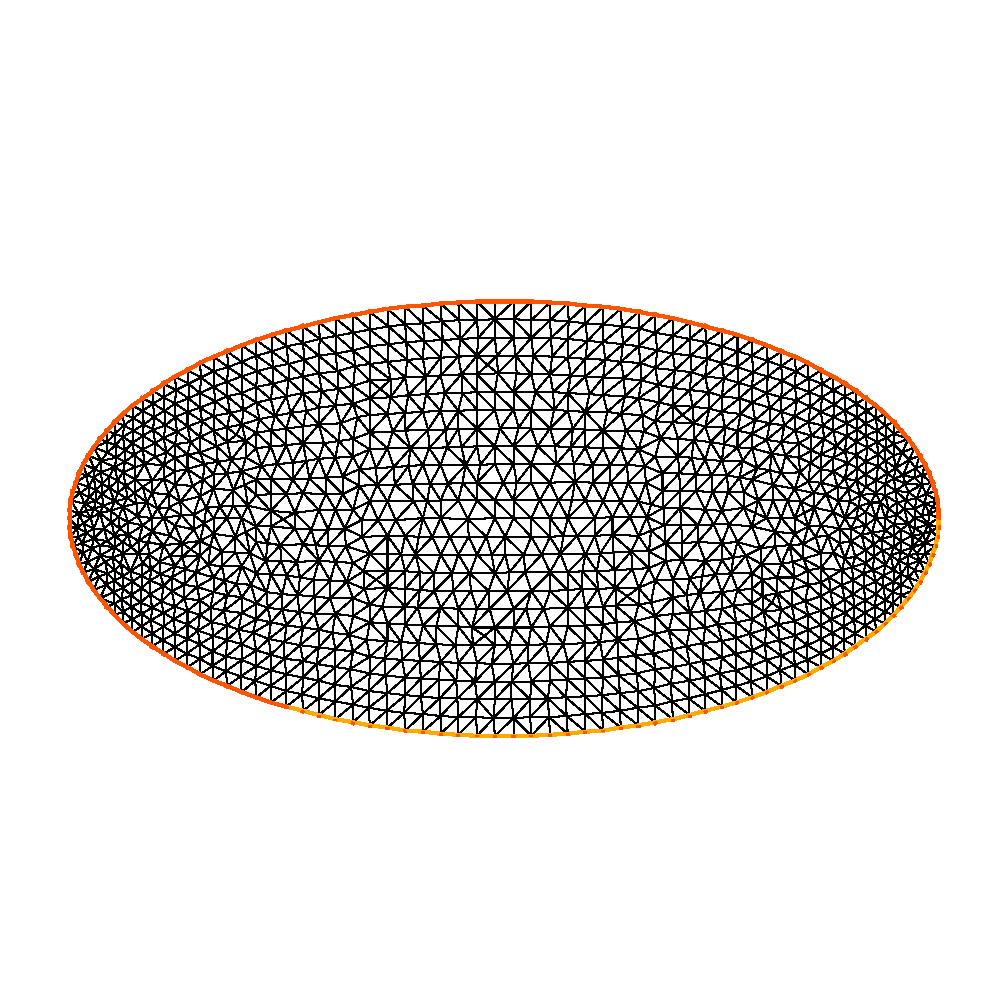
\includegraphics[width=7cm]{membraneTh}~~~
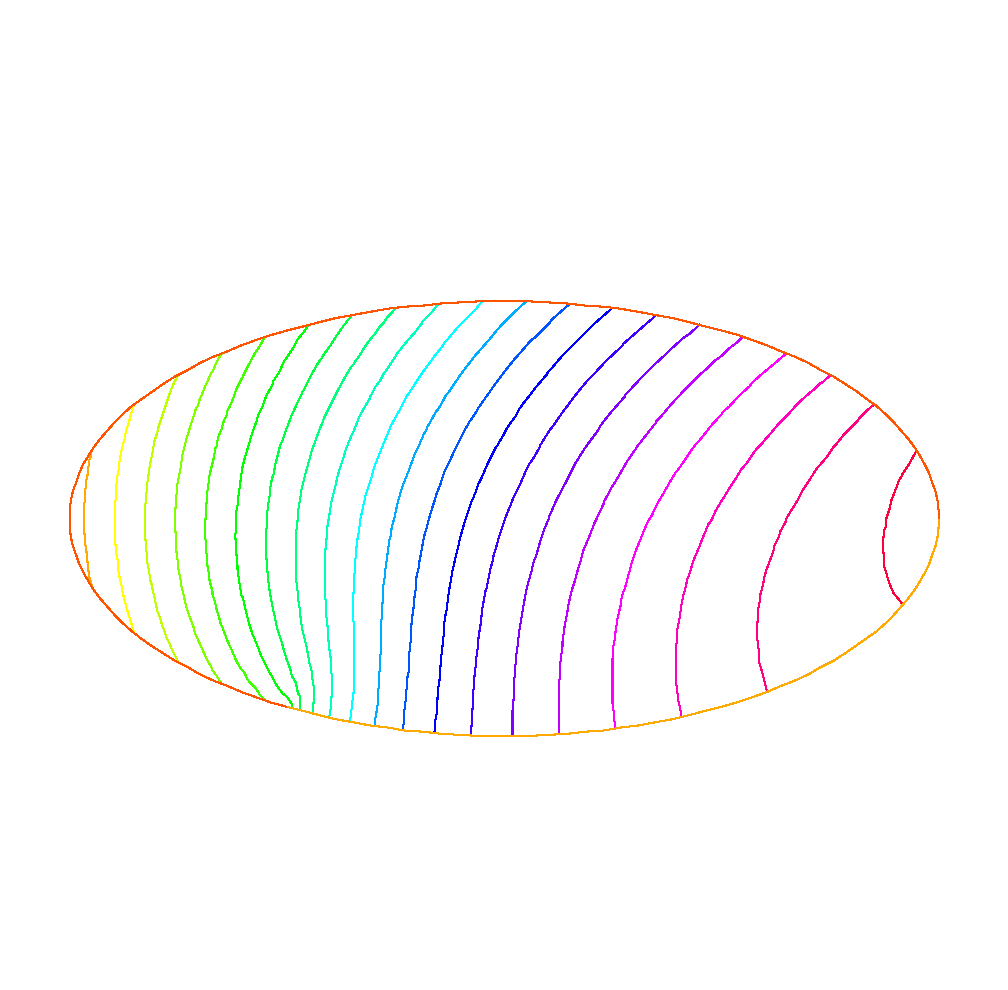
\includegraphics[width=7cm]{membrane}\\
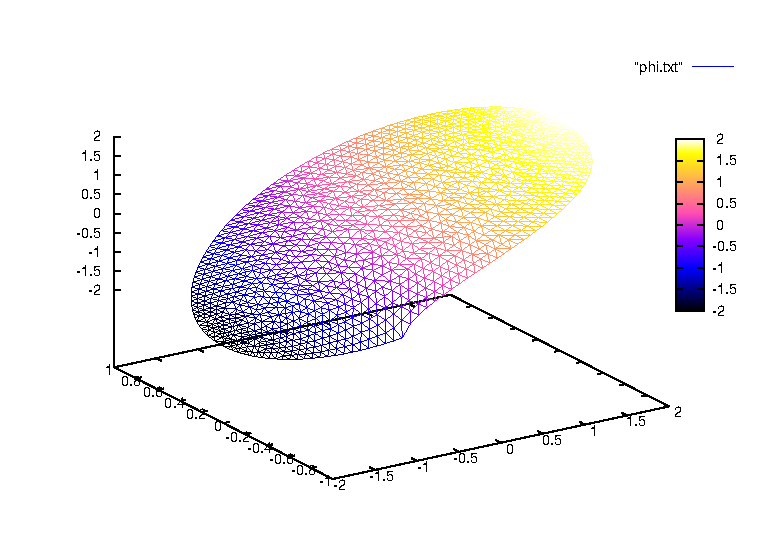
\includegraphics[width=12cm]{gnumembrane}\\
\caption{\label{figmembrane} Mesh and level lines of the membrane deformation. Below: the same in 3D
drawn by \texttt{gnuplot} from a file generated by \freefempp.}
\end{center}
\end{figure}

\index{buildmesh}
A triangulation is built by the keyword \ttCC{buildmesh}. This keyword
calls a triangulation subroutine based on the Delaunay test, which
first triangulates with only the boundary points, then adds internal
points by subdividing the edges. How fine  the triangulation becomes is controlled
by the size of the closest boundary edges.

\medskip

The PDE is then discretized using the triangular second order finite
element method on the triangulation; as was briefly indicated in the previous chapter,
a linear system is derived from the discrete formulation whose size is the number of vertices
plus the number of mid-edges in
the triangulation. The system is solved by a multi-frontal Gauss LU factorization
implemented in the package \texttt{UMFPACK}. The keyword plot will display both
$\T_h$ and $\varphi$ (remove \texttt{Th} if $\varphi$ only is desired) and the
qualifier \texttt{fill=true} replaces the default option (colored level lines) by a full color display.
Results are on figure \ref{figmembrane}.

\bFF
@plot(phi,wait=true,fill=true); //Plot phi with full color display
\eFF

Next we would like to check the results!
\\
One simple way is to adjust the parameters so as to know the solutions.  For instance
on the unit circle \texttt{a=1} , $\varphi_e=\sin(x^2+y^2-1)$ solves the problem when
\[
    z=0,~f=-4(\cos(x^2+y^2-1)-(x^2+y^2)\sin(x^2+y^2-1))
\]
except that on $\Gamma_2$ $\p_n\varphi=2$ instead of zero.  So we will consider
a non-homogeneous Neumann condition and solve
$$
    \int_\Omega(\n\varphi\cdot\n w = \int_\Omega f w+\int_{\Gamma_2}2w\quad\forall w\in V
$$
We will do that with two triangulations, compute the $L^2$ error:
\[
\epsilon = \int_\Omega|\varphi-\varphi_e|^2
\]
and print the error in both cases as well as the log of their ratio an indication of
the rate of convergence.
\begin{example}[membranerror.edp]\label{membran}
\bFF
// file membranerror.edp
verbosity =0; // to remove all default output
@real theta=4.*pi/3.;
@real a=1.,b=1.; // the length of the semimajor axis and  semiminor axis
@border Gamma1(t=0,theta)    { x = a * cos(t); y = b*sin(t); }
@border Gamma2(t=theta,2*pi) { x = a * cos(t); y = b*sin(t); }

@func f=-4*(cos(x^2+y^2-1) -(x^2+y^2)*sin(x^2+y^2-1));
@func phiexact=sin(x^2+y^2-1);

@real[int] L2error(2);  // an array two values
@for(@int n=0;n<2;n++)
{
  @mesh Th=buildmesh(Gamma1(20*(n+1))+Gamma2(10*(n+1)));
  @fespace Vh(Th,P2);
   Vh phi,w;

  @solve laplace(phi,w)=int2d(Th)(dx(phi)*dx(w) + dy(phi)*dy(w))
    - int2d(Th)(f*w) - int1d(Th,Gamma2)(2*w)+ on(Gamma1,phi=0);
  @plot(Th,phi,wait=true,ps="membrane.eps"); //Plot Th and phi

  L2error[n]= sqrt(int2d(Th)((phi-phiexact)^2));
}

@for(int n=0;n<2;n++)
 @cout << " L2error " << n << " = "<<  L2error[n] <<endl;

@cout <<" convergence rate = "<< log(L2error[0]/L2error[1])/log(2.)  <<endl;

\eFF
\end{example}

the output is
\bFF

 L2error 0 = 0.00462991
 L2error 1 = 0.00117128
 convergence rate = 1.9829
times: compile 0.02s, execution 6.94s
\eFF

We find a rate of $1.93591$, which is not close enough to the $3$ predicted by the theory.
The Geometry is always a polygon so we lose one order due to the geometry approximation in $O(h^2)$

%\paragraph{Quiz} Why is it not 3? (hint: this is not due to \freefempp, but to the theory itself).
%\\\\

\medskip
Now if you are not satisfied with the \texttt{.eps} plot generated by \freefempp and you want to use other graphic
facilities, then you must store the solution in a file very much like in \texttt{C++}. It will be useless
if you don't save the triangulation as well, consequently you must do
\bFF
     {
       @ofstream ff("phi.txt");
       ff << phi[];
      }
    @savemesh(Th,"Th.msh");
\eFF
For the triangulation the name is important: it is the extension that determines the format.
\\
Still that may not take you where you want. Here is an interface with gnuplot to produce the
right part of figure \ref{membran}.
\bFF
// to build a gnuplot data file
{ @ofstream ff("graph.txt");
   @for (@int i=0;i<Th.nt;i++)
   { @for (@int j=0; j <3; j++)
       ff<<Th[i][j].x  << "    "<< Th[i][j].y<< "  "<<phi[][Vh(i,j)]<<@endl;
    ff<<Th[i][0].x  << "    "<< Th[i][0].y<< "  "<<phi[][Vh(i,0)]<<"\n\n\n"
   }
}
\eFF
We use the finite element numbering, where \ttCC{Wh(i,j)} is the global index of
$j^{Th}$  degrees of freedom of triangle number $i$.

Then open \texttt{gnuplot} and do
\bFF
        set palette rgbformulae 30,31,32
        splot "graph.txt" w l pal
\eFF
This works with \ttCC{P2} and \ttCC{P1}, but not with \ttCC{P1nc}
because the 3 first degrees of freedom  of  \ttCC{P2} or \ttCC{P2} are on vertices
and not with \ttCC{P1nc}.




\subsection{Heat Exchanger}

\paragraph{Summary}\emph{ Here we shall learn more about \x{geometry input }and
\x{triangulation files, as well as read and write} operations.}

\paragraph{The problem}
Let $\{C_{i}\}_{1,2} $, be  2 thermal conductors within an enclosure
$C_0$.
The first one is held at a constant temperature ${u} _{1} $ the other one has a given thermal
conductivity $\kappa_2$ 5 times larger than the one of $C_0$.
We assume that the border of enclosure $C_0$ is held at temperature $20^\circ C$ and that
we have waited long enough for thermal equilibrium.

In order to know ${u} (x) $ at any point $x$ of the domain
$\Omega$, we must solve \\
 $$
 \n\cdot(\kappa\n{u})  =0 ~~ \hbox{ in }~\Omega,
 \quad {u}_{|\Gamma} =g
  $$
where $\Omega$ is the interior of $C_0$ minus the conductors $C_1$
and $\Gamma$ is the boundary of $\Omega$, that is $C_0\cup C_1 $
Here $g$ is any function of $x$ equal to  ${u}_i$ on $C_i$.
The second equation is a reduced form for: \\
$$
  {u} ={u} _{i}   \hbox{   on  }   ~~~C_{i}, \quad i=0,1.
$$
The variational formulation for this problem is in the subspace $H^1_0(\Omega)
\subset H^1(\Omega)$ of functions which have zero traces on $\Gamma$.
\[
    u-g\in H^1_0(\Omega)~:~\int_\Omega\n u\n v =0~~~\forall v\in H^1_0(\Omega)
\]
Let us assume that $C_0$ is a circle of radius 5 centered at the origin,
% N=2 the number of exchanger ,
 $C_i$ are
rectangles, $C_1$ being at the constant temperature $u_1=60^\circ C$.


%The mesh can be made by the following \freefempp script:

\begin{example}[heatex.edp]
\bFF
// file heatex.edp
@int C1=99, C2=98; // could be anything such that $\ne 0$ and $ C1 \ne C2$
@border C0(t=0,2*pi){x=5*cos(t); y=5*sin(t);}

@border C11(t=0,1){ x=1+t;  y=3;      label=C1;}
@border C12(t=0,1){ x=2;    y=3-6*t;  label=C1;}
@border C13(t=0,1){ x=2-t;  y=-3;     label=C1;}
@border C14(t=0,1){ x=1;    y=-3+6*t; label=C1;}

@border C21(t=0,1){ x=-2+t; y=3;      label=C2;}
@border C22(t=0,1){ x=-1;   y=3-6*t;  label=C2;}
@border C23(t=0,1){ x=-1-t; y=-3;     label=C2;}
@border C24(t=0,1){ x=-2;   y=-3+6*t; label=C2;}

@plot(    C0(50)            // to see the border of the domain
        + C11(5)+C12(20)+C13(5)+C14(20)
        + C21(-5)+C22(-20)+C23(-5)+C24(-20),
        wait=true, ps="heatexb.eps");

@mesh Th=@buildmesh(    C0(50)
                    + C11(5)+C12(20)+C13(5)+C14(20)
                    + C21(-5)+C22(-20)+C23(-5)+C24(-20));
@plot(Th,wait=1);

@fespace Vh(Th,P1); Vh u,v;
Vh kappa=1+2*(x<-1)*(x>-2)*(y<3)*(y>-3);
@solve a(u,v)= @int2d(Th)(kappa*(@dx(u)*@dx(v)+@dy(u)*@dy(v)))
                +@on(C0,u=20)+@on(C1,u=60);
@plot(u,wait=true, value=true, fill=true, ps="heatex.eps");
\eFF
\end{example}

Note the following:
\begin{itemize}
\item \texttt{C0} is oriented counterclockwise by $t$, while   \texttt{C1} is oriented clockwise
     and \texttt{C2} is oriented counterclockwise.
    This is why \texttt{C1} is viewed as a hole by {\tt buildmesh}.
%
\item \texttt{C1} and \texttt{C2} are built by joining pieces of straight lines.  To group them in the
    same logical unit to input the boundary conditions in a readable way we
    assigned a \x{label on the boundaries}.  As said earlier, borders
    have an internal number corresponding to their order in the program (check it by
    adding a {\tt cout<<C22;} above). This is essential to understand how a mesh can be
    output to a file and re-read (see below).
%
\item As usual the mesh density is controlled by the number of vertices assigned to each
    boundary. It is not possible to change the (uniform) distribution of vertices but a
    piece of boundary can always be cut in two or more parts, for instance \texttt{C12} could be
    replaced by \texttt{C121+C122}:

\bFF
 //    border C12(t=0,1){ x=2;    y=3-6*t;   label=C1;}
    @border C121(t=0,0.7){ x=2;    y=3-6*t;  label=C1;}
    @border C122(t=0.7,1){ x=2;    y=3-6*t;  label=C1;}
    ... @buildmesh(.../* C12(20) */ + C121(12)+C122(8)+...);
\eFF
\end{itemize}

\begin{figure}[htbp]
\begin{center}
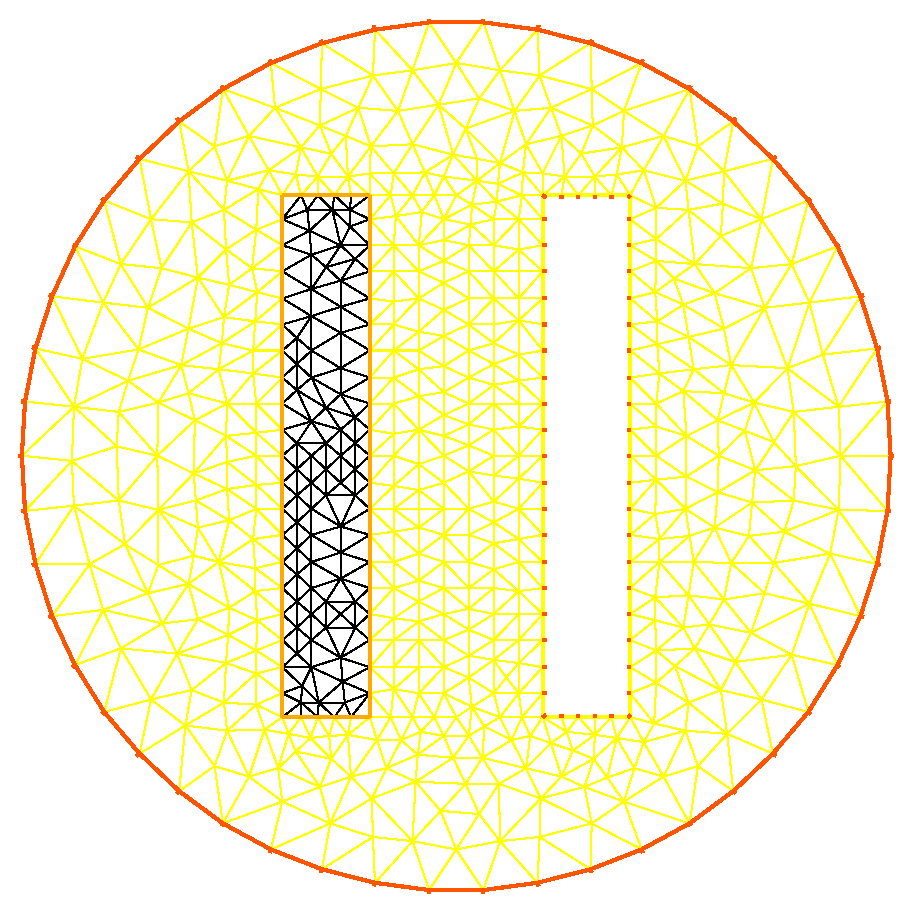
\includegraphics[width=6cm]{heatexTh}~~~
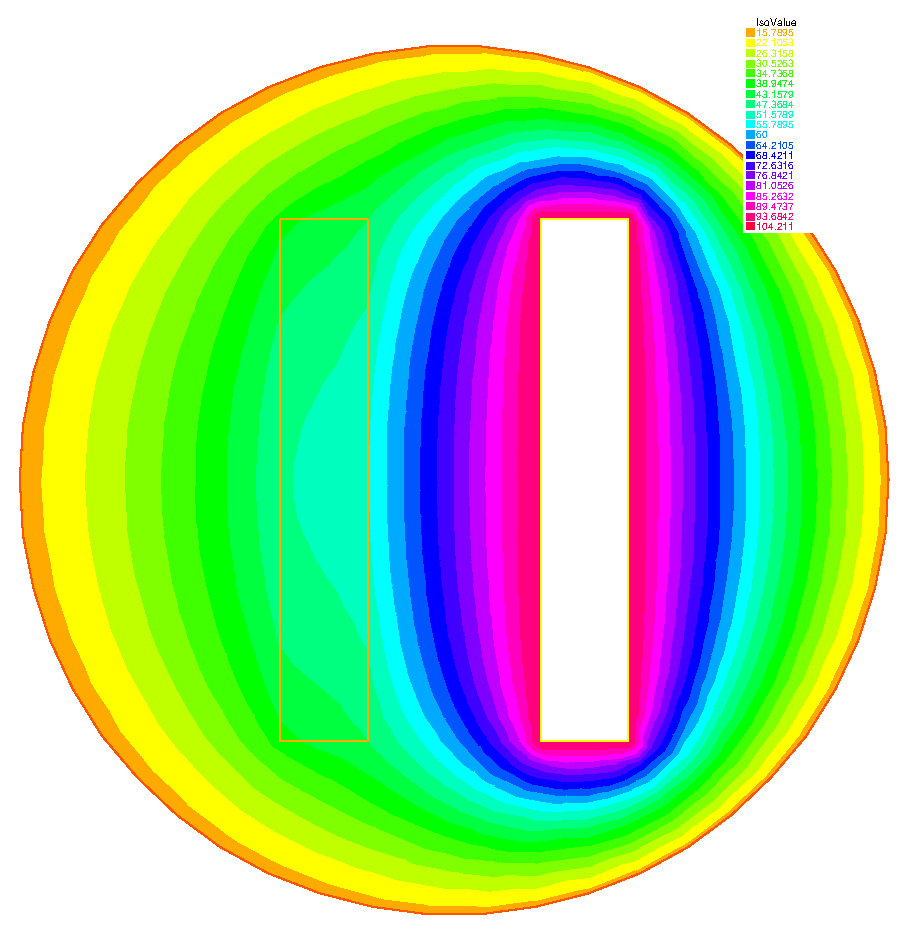
\includegraphics[width=6cm]{heatex}
\caption{\label{figheatex} The heat exchanger}
\end{center}
\end{figure}

\paragraph{Exercise} Use the symmetry of the problem with respect to the axes;
triangulate only one half of the domain, and set \x{Dirichlet}
conditions on the vertical axis, and Neumann conditions on the
horizontal axis.%\fin

\bigskip

\paragraph{Writing and reading triangulation files}
Suppose that at the end of the previous program we added the line
\bFF
savemesh(Th,"condensor.msh");
\eFF
and then later on we write a similar program but we wish to read the mesh from that
file. Then this is how the condenser should be computed:
\bFF
@mesh Sh=@readmesh("condensor.msh");
fespace Wh(Sh,P1); Wh us,vs;
@solve b(us,vs)= @int2d(Sh)(@dx(us)*@dx(vs)+@dy(us)*@dy(vs))
                +@on(1,us=0)+@on(99,us=1)+@on(98,us=-1);
@plot(us);
\eFF
Note that the names of the boundaries are lost but either their internal number
(in the case of \texttt{C0}) or their label number (for \texttt{C1} and \texttt{C2}) are kept.


 \subsection{Acoustics}

\paragraph{Summary}
\emph{Here we go to grip with \x{ill posed problems} and \x{eigenvalue problems}}

Pressure variations in air at rest are governed by the wave equation:
\[
     {\p^2 u \over \p t^2} - c^2 \Delta u =0.
\]
When the solution wave is monochromatic (and that depend on the boundary and initial conditions),
 $u$ is of the form
$u(x,t)=Re(v(x) e^{ik t})$ where $v$ is a solution of Helmholtz's equation:
%
\begin{eqnarray}&&
 k ^{2}v  + c^{2}\Delta v  =0 ~\hbox{~in~}~~\Omega,
 \cr&&
 \frac{\p v}{\p n}|_\Gamma=g.
\end{eqnarray}
%
where $g$ is the source.
Note the ``+'' sign in front of the Laplace operator and that $k>0$ is real. This sign may make the
problem ill posed for some values of $\frac c k$, a phenomenon called
 ``resonance''.\\
At resonance there are non-zero solutions even when $g=0$. So the following program may or may not work:

\begin{example}[sound.edp]
\bFF
// file sound.edp
@real kc2=1;
@func g=y*(1-y);

@border a0(t=0,1) { x= 5; y= 1+2*t ;}
@border a1(t=0,1) { x=5-2*t; y= 3 ;}
@border a2(t=0,1) { x= 3-2*t; y=3-2*t ;}
@border a3(t=0,1) { x= 1-t; y= 1 ;}
@border a4(t=0,1) { x= 0; y= 1-t ;}
@border a5(t=0,1) { x= t; y= 0  ;}
@border a6(t=0,1) { x= 1+4*t; y= t ;}

@mesh Th=@buildmesh( a0(20) + a1(20) + a2(20)
        + a3(20) + a4(20) + a5(20) + a6(20));
@fespace Vh(Th,P1);
Vh u,v;

solve sound(u,v)=@int2d(Th)(u*v * kc2 - @dx(u)*@dx(v) - @dy(u)*@dy(v))
                 - @int1d(Th,a4)(g*v);
@plot(u, wait=1, ps="sound.eps");
\eFF
\end{example}

Results are on Figure \ref{figsound}.  But when $kc2$ is an eigenvalue of the problem, then the
solution is not unique:
%%%ALH- \nequiv not available when package txfonts is disabled
if $u_e \neq 0$ is an eigen state, then for any given solution $u+u_e$ is another  a solution.
%$u_e$ the eigen state, "u" a solution $\Rightarrow$ $u+u_e$ is also a solution.
To find all the $u_e$ one can do the following
\bFF
@real sigma = 20;  // value of the shift
// OP = A - sigma B ;  //  the shifted matrix
@varf  op(u1,u2)= @int2d(Th)(  @dx(u1)*@dx(u2) + @dy(u1)*@dy(u2) - sigma* u1*u2 );
@varf b([u1],[u2]) = @int2d(Th)( u1*u2 ) ;//no Boundary condition see note \ref{note BC EV}

@matrix OP= op(Vh,Vh,solver=Crout,factorize=1);
@matrix B= b(Vh,Vh,solver=CG,eps=1e-20);

@int nev=2;  // number of requested eigenvalues near sigma

@real[int] ev(nev); // to store the  nev eigenvalue
Vh[int] eV(nev);   // to store the nev eigenvector

@int k=EigenValue(OP,B,sym=true,sigma=sigma,value=ev,vector=eV,
                   tol=1e-10,maxit=0,ncv=0);
@cout<<ev(0)<<" 2 eigen values "<<ev(1)<<endl;
v=eV[0];
@plot(v,wait=1,ps="eigen.eps");
\eFF
\begin{figure}[htbp]
\begin{center}
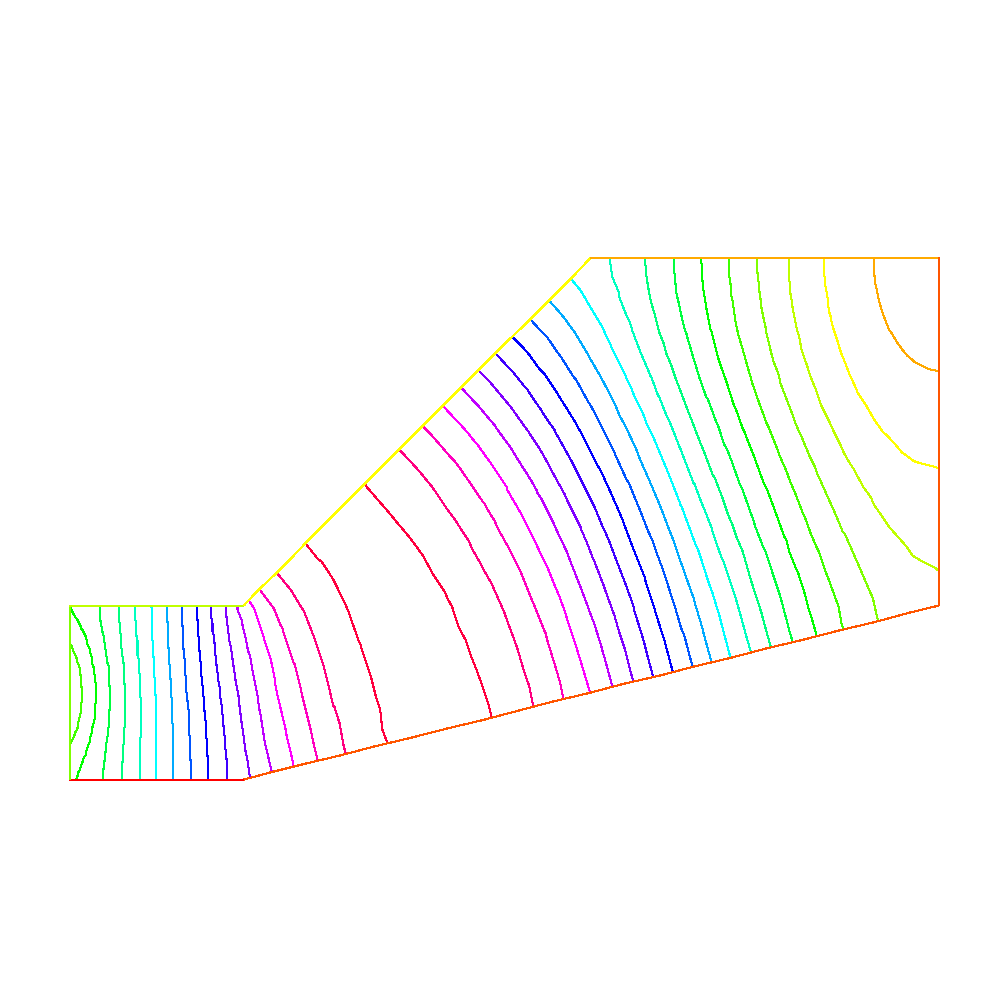
\includegraphics[width=8cm]{sound0}~~~
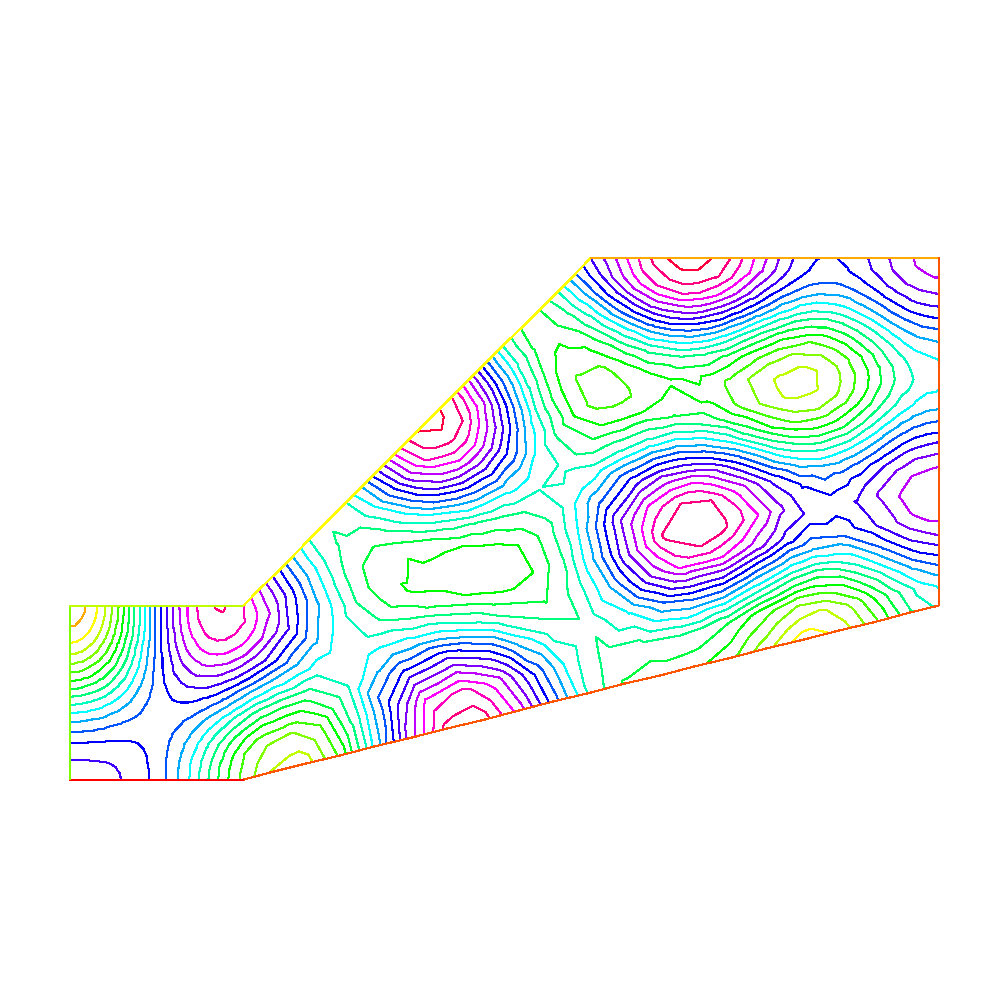
\includegraphics[width=8cm]{eigen}

\caption{\label{figsound}Left:Amplitude of an acoustic signal coming from the left vertical wall.
Right:  first eigen state ($\lambda=(k/c)^2=19.4256$) close to $20$ of eigenvalue problem :$ -\Delta \varphi = \lambda \varphi$ and $ \frac{\partial \varphi}{\partial n} = 0$ on $\Gamma$}
\end{center}
\end{figure}

\subsection{Thermal Conduction}
\label{ss Thermal Conduction}
\paragraph{Summary}\emph{ Here we shall learn how to deal with a \x{
time dependent} \x{parabolic} problem. We shall also show how to treat an
\x{axisymmetric} problem  and show also how to deal with a \x{nonlinear problem}.}

\paragraph{How air cools a plate}

We seek the temperature distribution in a plate $(0,Lx)\times(0,Ly)\times(0,Lz)$
of rectangular cross section $\Omega=(0,6)\times(0,1)$; the plate is
surrounded by air at temperature $u_e$ and
initially at temperature $u=u_0+\frac x L u_1$. In the plane perpendicular to the plate
at $z=Lz/2$,  the temperature varies little with
the coordinate $z$; as a first approximation the problem is 2D.
\\\\
We must solve the temperature equation in $\Omega$ in a time interval (0,T).
\begin{eqnarray}&&
    \p_t u -\n\cdot(\kappa\n u)=0 \hbox{ in } \Omega\times(0,T),
    \cr&&
    u(x,y,0)=u_0+x u_1
    \cr&&
    \kappa\frac{\p u}{\p n} +\alpha(u-u_e)=0\hbox{ on } \Gamma\times(0,T).
\end{eqnarray}
Here the diffusion $\kappa$ will take two values, one below the middle horizontal line and ten times less
above, so as to simulate a thermostat.
The term $\alpha(u-u_e)$ accounts for the loss of temperature by convection in air.  Mathematically
this boundary condition is of \x{Fourier} (or \x{Robin}, or \x{mixed}) type.
\\
The variational formulation is  in $L^2(0,T;H^1(\Omega))$; in loose terms and after applying an implicit Euler
finite difference approximation in time; we shall seek $u^n(x,y)$ satisfying for all $w\in H^1(\Omega)$:
\[
    \int_\Omega(\frac{u^n-u^{n-1}}{\delta t} w + \kappa\n u^n\n w) +\int_\Gamma\alpha(u^n-u_ue)w=0
\]
\bFF
@func u0 =10+90*x/6;
@func k = 1.8*(y<0.5)+0.2;
@real ue = 25, alpha=0.25, T=5, dt=0.1 ;

@mesh Th=@square(30,5,[6*x,y]);
@fespace Vh(Th,P1);
Vh u=u0,v,uold;

@problem thermic(u,v)= @int2d(Th)(u*v/dt + k*(@dx(u) * @dx(v) + @dy(u) * @dy(v)))
                + @int1d(Th,1,3)(alpha*u*v)
                - @int1d(Th,1,3)(alpha*ue*v)
                - @int2d(Th)(uold*v/dt) + @on(2,4,u=u0);
@ofstream ff("thermic.dat");
@for(@real t=0;t<T;t+=dt){
    uold=u;    // uold $\equiv  u^{n-1} = u^n \equiv $u \hfilll
    thermic;  // here solve the thermic problem \hfilll
    ff<<u(3,0.5)<<@endl;
    @plot(u);
}
\eFF
Notice that we must separate by hand the bilinear part from the linear one.

Notice also that  the way we store the temperature at point (3,0.5) for all times in file {\tt thermic.dat}.
Should a one dimensional plot be required, the same procedure can be used.  For instance to
print $x\mapsto \frac{\p u}{\p y}(x,0.9)$ one would do
\bFF
@for(@int i=0;i<20;i++) @cout<<@dy(u)(6.0*i/20.0,0.9)<<@endl;
\eFF
Results are shown on Figure \ref{figthermic}.

\begin{figure}[htbp]
\begin{center}
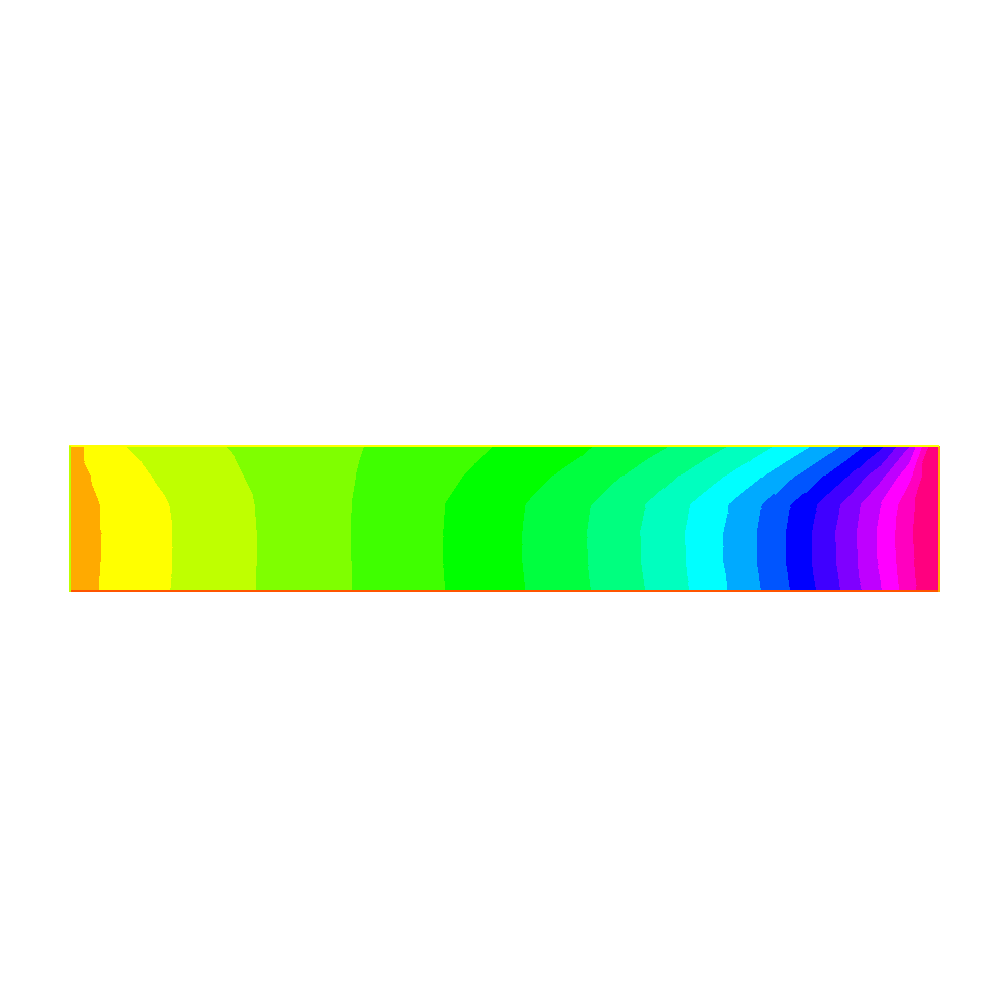
\includegraphics[width=8cm]{thermic}~~~
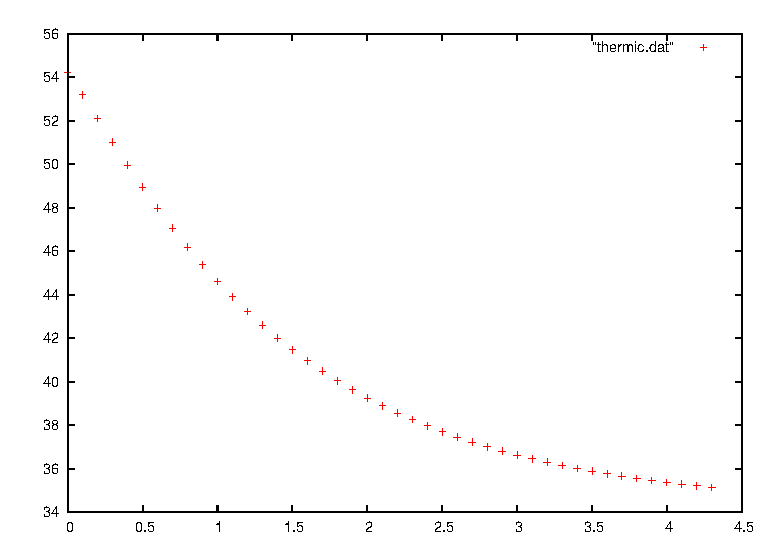
\includegraphics[width=8cm]{thermicvst}

\caption{\label{figthermic} Temperature at T=4.9. Right: decay of temperature versus time at x=3, y=0.5}
\end{center}
\end{figure}

\subsubsection{Axisymmetry: 3D Rod with circular section}

Let us now deal with a cylindrical rod instead of a flat plate.  For simplicity we take $\kappa=1$.
In cylindrical coordinates, the Laplace
operator becomes ($r$ is the distance to the axis, $z$ is the distance along the
axis, $\theta$ polar angle in a fixed plane perpendicular to the axis):

$$ \Delta u = {1\over r}\p _r(r\p _r u) + {1\over r^2}\p ^2_{\theta\theta} u
 + \p ^2_{z z}.
$$

Symmetry implies that we loose the dependence with respect to
$\theta$; so the domain $\Omega$ is again a rectangle $]0,R[\times]0,|[$ . We take the convention of
numbering of the edges as in {\tt square()} (1 for the bottom horizontal ...);
the problem is now:

\begin{eqnarray}&&
r\p_t u-\p _r(r\p _r u) - \p _z(r\p _z u) = 0 \hbox{ in } \Omega,
\cr&&
u(t=0) = u_0 + \frac z{L_z} (u_1-u)
\cr&&
u|_{\Gamma_4} = u_0,\quad  u|_{\Gamma_2} = u_1,
\quad \alpha(u-u_e) + {\p u\over \p n} |_{\Gamma_1\cup\Gamma_3} = 0.
\end{eqnarray}
Note that the PDE has been multiplied by $r$.

After discretization in time with an implicit scheme, with time steps \texttt{dt},
in the \freefempp syntax $r$ becomes $x$ and $z$ becomes $y$ and the problem is:
\bFF
@problem thermaxi(u,v)=@int2d(Th)((u*v/dt + @dx(u)*@dx(v) + @dy(u)*@dy(v))*x)
                + @int1d(Th,3)(alpha*x*u*v) - @int1d(Th,3)(alpha*x*ue*v)
                - @int2d(Th)(uold*v*x/dt) + @on(2,4,u=u0);
\eFF
Notice that the bilinear form degenerates at $x=0$. Still one can prove existence and uniqueness
for $u$ and because of this degeneracy no boundary conditions need to be imposed on $\Gamma_1$.

\subsubsection{A Nonlinear Problem : Radiation}

Heat loss through \x{radiation}  is a loss proportional
to the absolute temperature to the fourth power (Stefan's Law). This adds to the
loss by convection and gives the following
boundary condition:
 $$\kappa{\p u\over \p n} +\alpha(u-u_e) + c[(u + 273)^4 - (u_e+273)^4] = 0$$

The problem is \x{nonlinear}, and must be solved iteratively. If $m$
denotes the iteration index, a semi-linearization of the radiation condition gives
$${\p u^{m+1}\over \p n} + \alpha(u^{m+1}-u_e)+ c(u^{m+1}-u_e)
(u^m+u_e +546) ((u^m + 273)^2 + (u_e+273)^2)  = 0,
$$
because we have the identity
$ a^4 - b^4 = (a-b)(a+b)(a^2+b^2)$.
The iterative process will work with $v=u-u_e$.
\bFF
...
@fespace Vh(Th,P1);  //  finite element space
@real rad=1e-8, uek=ue+273; // def of the physical constants
Vh vold,w,v=u0-ue,b;
@problem thermradia(v,w)
    = @int2d(Th)(v*w/dt + k*(@dx(v) * @dx(w) + @dy(v) * @dy(w)))
                + @int1d(Th,1,3)(b*v*w)
                - @int2d(Th)(vold*w/dt) + @on(2,4,v=u0-ue);

@for(@real t=0;t<T;t+=dt){
    vold=v;
    @for(@int m=0;m<5;m++){
       b= alpha + rad * (v + 2*uek) * ((v+uek)^2 + uek^2);
       thermradia;
    }
}
vold=v+ue; @plot(vold);
\eFF


\subsection{Irrotational Fan Blade Flow and Thermal effects}

\paragraph{Summary}\emph{Here we will learn how to deal with a \x{multi-physics system}
of PDEs on a \x{Complex geometry,} with \x{multiple meshes} within one problem.  We
also learn how to manipulate the \x{region indicator} and see how smooth is the projection
operator from one mesh to another.}

 \paragraph{Incompressible flow}

Without viscosity and vorticity incompressible flows have a velocity given by:
 $$
 u=\left(\begin{matrix}{\p \psi \over \p x_{2} }\\ -{\p \psi
 \over \p x_{1}} \end{matrix}\right), \quad
  \hbox{  where $\psi  $ is solution of }\quad  \Delta \psi =0
$$
This equation expresses both incompressibility
 ($\nabla\cdot u=0$) and absence of vortex ($\nabla\times u =0$).

As the fluid slips along the walls, normal velocity is zero, which
means that $\psi$ satisfies:
$$
 \psi \hbox{ constant on the walls}.
$$
One can also prescribe the normal velocity at an artificial boundary, and this translates into
 non constant {Dirichlet} data for $\psi$.
\\\\

\paragraph{Airfoil}

Let us consider a wing profile $S$ in a uniform flow. Infinity will be
represented by a large circle  $C$ where the flow is assumed to be of uniform velocity;
one way to model this problem is to write
 \begin{eqnarray}&&
 \Delta \psi =0 ~\hbox{~in~}~ \Omega, \qquad
 \psi |_{S}=0, \quad
 \psi|_{C}= {u_\infty}y,
\end{eqnarray}
 where $\partial\Omega=C\cup S $

\paragraph{The NACA0012 Airfoil}
An equation for the upper surface of a NACA0012 (this is a classical
  wing profile in aerodynamics) is:
$$    y = 0.17735\sqrt{x}-0.075597x- 0.212836x^2+0.17363x^3-0.06254x^4.$$
%
\begin{example}[potential.edp]
\bFF
// file potential.edp

@real S=99;
@border C(t=0,2*pi) {  x=5*cos(t);  y=5*sin(t);}
@border Splus(t=0,1){  x = t; y = 0.17735*sqrt(t)-0.075597*t
        - 0.212836*(t^2)+0.17363*(t^3)-0.06254*(t^4); label=S;}
@border Sminus(t=1,0){  x =t; y= -(0.17735*sqrt(t)-0.075597*t
        -0.212836*(t^2)+0.17363*(t^3)-0.06254*(t^4)); label=S;}
@mesh Th= @buildmesh(C(50)+Splus(70)+Sminus(70));
@fespace Vh(Th,P2); Vh psi,w;

@solve potential(psi,w)=@int2d(Th)(@dx(psi)*@dx(w)+@dy(psi)*@dy(w))+
  @on(C,psi = y) + @on(S,psi=0);

@plot(psi,wait=1);

\eFF
\end{example}

A zoom of the streamlines are shown on Figure \ref{figpotential}.

\begin{figure}[htbp]
\begin{center}
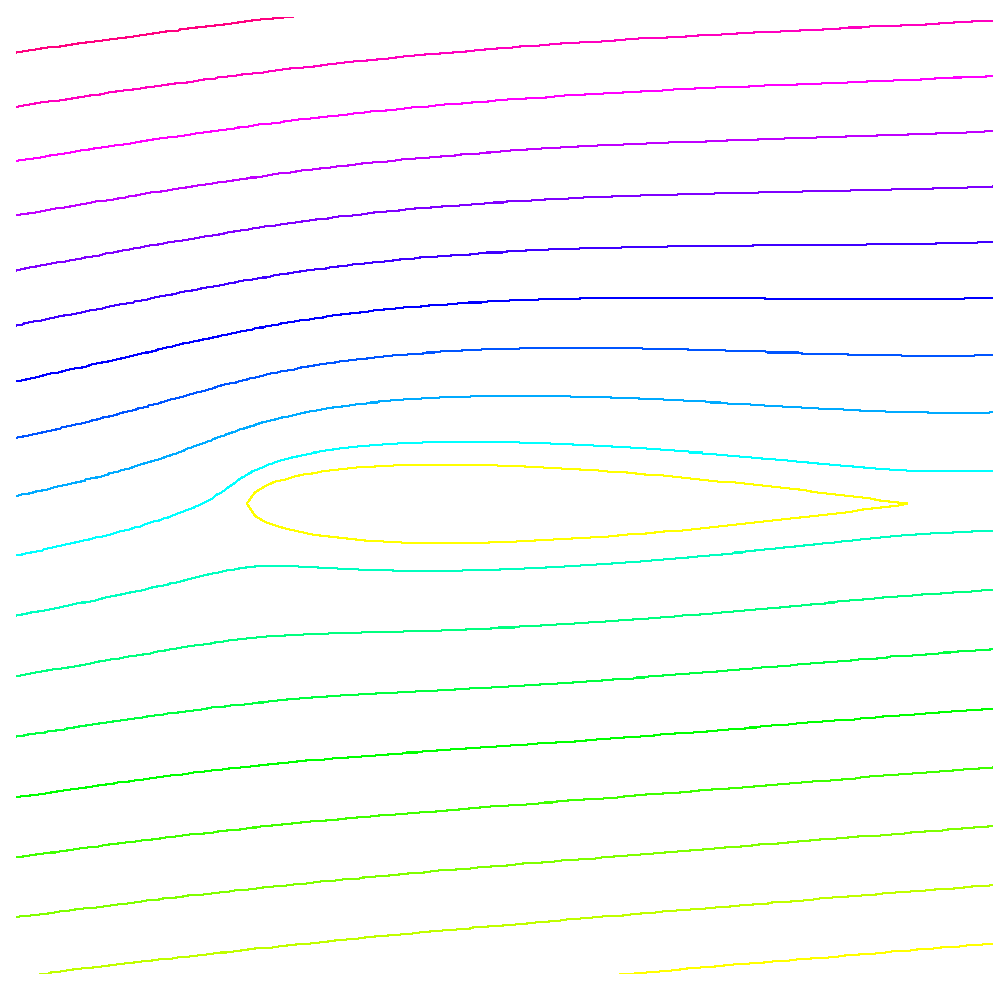
\includegraphics[width=8cm]{potential}
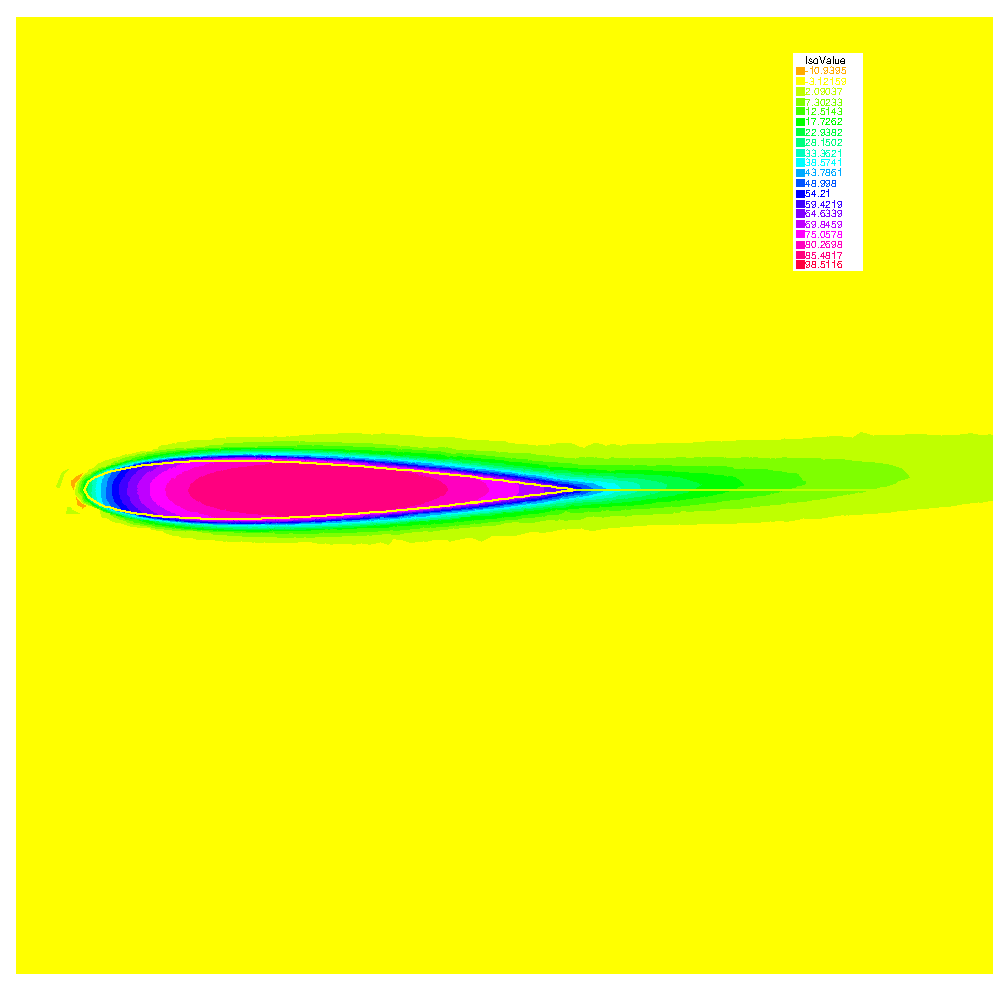
\includegraphics[width=8cm]{potheat}

\caption{\label{figpotential} Zoom around the NACA0012 airfoil showing the streamlines (curve $\psi=$ constant).
To obtain such a plot use the interactive graphic command: ``+" and p.
Right: temperature distribution at time T=25 (now the maximum is at 90 instead of 120).
Note that an incidence angle has been added here (see Chapter 9).}
\end{center}
\end{figure}

 \subsubsection{Heat Convection around the airfoil}
Now let us assume that the airfoil is hot and that air is there to cool it.
Much like in the previous section the heat equation for the temperature $v$ is
$$
\p_t v -\n\cdot(\kappa\n v) + u\cdot\n v =0,~~v(t=0)=v_0, ~~\frac{\p v}{\p n}|_C=0
$$
But now the domain is outside AND inside $S$ and $\kappa$ takes a different value in air
and in steel.  Furthermore there is convection of heat by the flow, hence the
term $u\cdot\n v$ above.  Consider the following, to be plugged at the end of the previous program:
\bFF
...
@border D(t=0,2){x=1+t;y=0;} // added to have a fine mesh at trail
@mesh Sh = @buildmesh(C(25)+Splus(-90)+Sminus(-90)+D(200));
@fespace Wh(Sh,P1); Wh v,vv;
@int steel=Sh(0.5,0).region, air=Sh(-1,0).region;
@fespace W0(Sh,P0);
W0 k=0.01*(@region==air)+0.1*(@region==steel);
W0 u1=@dy(psi)*(@region==air), u2=-@dx(psi)*(@region==air);
Wh vold = 120*(@region==steel);
@real dt=0.05, nbT=50;
@int i;
@problem thermic(v,vv,init=i,solver=LU)= @int2d(Sh)(v*vv/dt
                + k*(@dx(v) * @dx(vv) + @dy(v) * @dy(vv))
                + 10*(u1*@dx(v)+u2*@dy(v))*vv)- @int2d(Sh)(vold*vv/dt);
@for(i=0;i<nbT;i++){
    v=vold; thermic;
 @plot(v);
}
\eFF
Notice here
\begin{itemize}
\item how steel and air are identified by the mesh parameter region which is defined when buildmesh is
called and takes an integer value corresponding to each connected component of $\Omega$;

\item how the convection terms are added without upwinding. Upwinding is necessary when the
Pecley number $|u|L/\kappa$ is large (here is a typical length scale), The factor 10 in front of
the convection terms is a quick way of multiplying the velocity by 10 (else it is too slow to see something).

\item The solver is Gauss' LU factorization and when {\tt init}$\neq 0$ the LU decomposition is reused so it
is much faster after the first iteration.
\end{itemize}

\subsection{Pure Convection : The Rotating Hill}

\paragraph{Summary}\emph{ Here we will present two methods for \x{upwinding} for the simplest
convection problem.  We will learn about \x{Characteristics-Galerkin}
and \x{Discontinuous-Galerkin} Finite Element Methods.}

Let $\Omega$ be the unit disk centered at 0; consider the rotation vector field
$$ \bm{u} = [u1,u2], \qquad u_1 = y,\quad u_2 = -x.$$
Pure convection by $u$ is
$$
    \p_t c  + \bm{u}.\nabla c  = 0~\hbox{~in~}~~\Omega\times(0,T)
    ~~~ c (t=0) =  c ^0~\hbox{~in~}~~\Omega.
$$
The exact solution $c(x_t,t)$ at time $t$ en point $x_t$ is given by
$$
 c(x_t,t)=c^0(x,0)
$$
where $x_t$ is the particle path in the flow starting at point $x$ at time $0$.
So $x_t$ are solutions of
\[
    \dot{x_t} = u(x_t),~~~\vec  , \quad\ x_{t=0} =x , \quad\mbox{where}\quad  \dot{x_t} = \frac{\d ( t \mapsto x_t)}{\d t}
\]
The ODE are reversible and we want the solution at point $x$ at time $t$ ( not at point $x_t$)
the initial point is $x_{-t}$, and we have
$$
 c(x,t)=c^0(x_{-t},0)
$$
The game consists in solving the equation until $T=2\pi$, that is for
a full revolution and to compare the final solution with the initial one;
they should be equal.

\paragraph{Solution by a Characteristics-Galerkin Method} % modif FH 2008
In \freefempp there is an operator called {\tt convect([u1,u2],dt,c)} which compute  \index{convect}
$ c\circ X$ with $X$ is the convect field defined by
$ X(x)= x_{dt}$ and where  $x_\tau$ is particule path in the steady state velocity field $\bm{u}=[u1,u2]$
starting at point $x$ at time $\tau=0$, so $x_\tau$ is solution of the following ODE:
%exactly the equation for ${\vec \chi}:=(X(\tau),Y(\tau))$
\[
    \dot{x}_\tau = u(x_\tau),~~~\vec x_{\tau=0}=x.
\]

When $\bm{u}$ is piecewise constant; this is possible because
$x_\tau$ is then a polygonal curve which can be computed exactly and the solution exists always when
$u$ is divergence free; convect returns  $c(x_{df})=C\circ X$.
 % modif FH 2008
\begin{example}[convects.edp]
\bFF
// file convects.edp

@border C(t=0, 2*pi) { x=cos(t);  y=sin(t); };
@mesh Th = @buildmesh(C(100));
@fespace Uh(Th,P1);
Uh cold, c = exp(-10*((x-0.3)^2 +(y-0.3)^2));

@real dt = 0.17,t=0;
Uh u1 = y, u2 = -x;
@for (int m=0; m<2*pi/dt ; m++) {
    t += dt;     cold=c;
    c=@convect([u1,u2],-dt,cold);
    @plot(c,cmm=" t="+t + ", min=" + c[].min + ", max=" +  c[].max);
}

\eFF
\end{example}
\begin{remark}  3D plots can be done by adding the qualifyer "dim=3" to the plot instruction.
\end{remark}

The method is very powerful but has two limitations: a/ it is not conservative, b/ it may diverge
in rare cases when $|u|$ is too small due to quadrature error.

\paragraph{Solution by Discontinuous-Galerkin FEM}

Discontinuous Galerkin methods take advantage of the discontinuities of $c$ at the edges to build
upwinding.  There are may formulations possible. We shall implement here the so-called dual-$P_1^{DC}$
formulation (see Ern\cite{ern}):
\[
    \int_\Omega(\frac{c^{n+1}-c^n}{\delta t} +u\cdot\n c)w
    +\int_E(\alpha|n\cdot u|-\frac 12 n\cdot u)[c]w
    =\int_{E_\Gamma^-}|n\cdot u| cw~~~\forall w
\]
where $E$ is the set of inner edges and $E_\Gamma^-$ is the set of boundary edges where $u\cdot n<0$
(in our case there is no such edges). Finally $[c]$ is the jump of $c$ across an edge with the convention
that $c^+$ refers to the value on the right of the oriented edge.
\begin{example}[convects\_end.edp]
\bFF
// file convects.edp
...
@fespace Vh(Th,P1dc);

Vh w, ccold, v1 = y, v2 = -x, cc = exp(-10*((x-0.3)^2 +(y-0.3)^2));
@real u, al=0.5;  dt = 0.05;

@macro n() (N.x*v1+N.y*v2) // Macro without parameter \index{macro!without parameter}
@problem  Adual(cc,w) =
@int2d(Th)((cc/dt+(v1*@dx(cc)+v2*@dy(cc)))*w)
  + @intalledges(Th)((1-@nTonEdge)*w*(al*abs(n)-n/2)*@jump(cc))
//  - @int1d(Th,C)((n<0)*abs(n)*cc*w)  // unused because cc=0 on $\p\Omega^-$
  - @int2d(Th)(ccold*w/dt);

for ( t=0; t< 2*pi ; t+=dt)
{
  ccold=cc; Adual;
  @plot(cc,fill=1,cmm="t="+t + ", min=" + cc[].min + ", max=" +  cc[].max);
};
@real [int] viso=[-0.2,-0.1,0,0.1,0.2,0.3,0.4,0.5,0.6,0.7,0.8,0.9,1,1.1];
@plot(c,wait=1,fill=1,ps="convectCG.eps",viso=viso);
@plot(c,wait=1,fill=1,ps="convectDG.eps",viso=viso);

\eFF
\end{example}
Notice the new keywords, \texttt{intalledges} to integrate on all edges of all triangles
\begin{equation}
\mathtt{intalledges}(\mathtt{Th}) \equiv \sum_{T\in\mathtt{Th}}\int_{\p T }
\end{equation}

(so all internal edges are see two times ), \x{nTonEdge} which is one
if the triangle has a boundary edge and zero otherwise, {\tt jump} to implement $[c]$.
Results of both methods are shown on Figure \ref{figconvect} with identical levels for the \x{level line};
this is done with the plot-modifier \x{viso}.
\index{plot!viso=}

Notice also the  \x{macro} where the parameter $u$ is not used (but
the syntax needs one) and which ends with a //; it simply replaces
the name {\tt n} by {\tt (N.x*v1+N.y*v2)}. As easily guessed {\tt
N.x,N.y} is the \x{normal} to the edge.

\begin{figure}[htbp]
\begin{center}
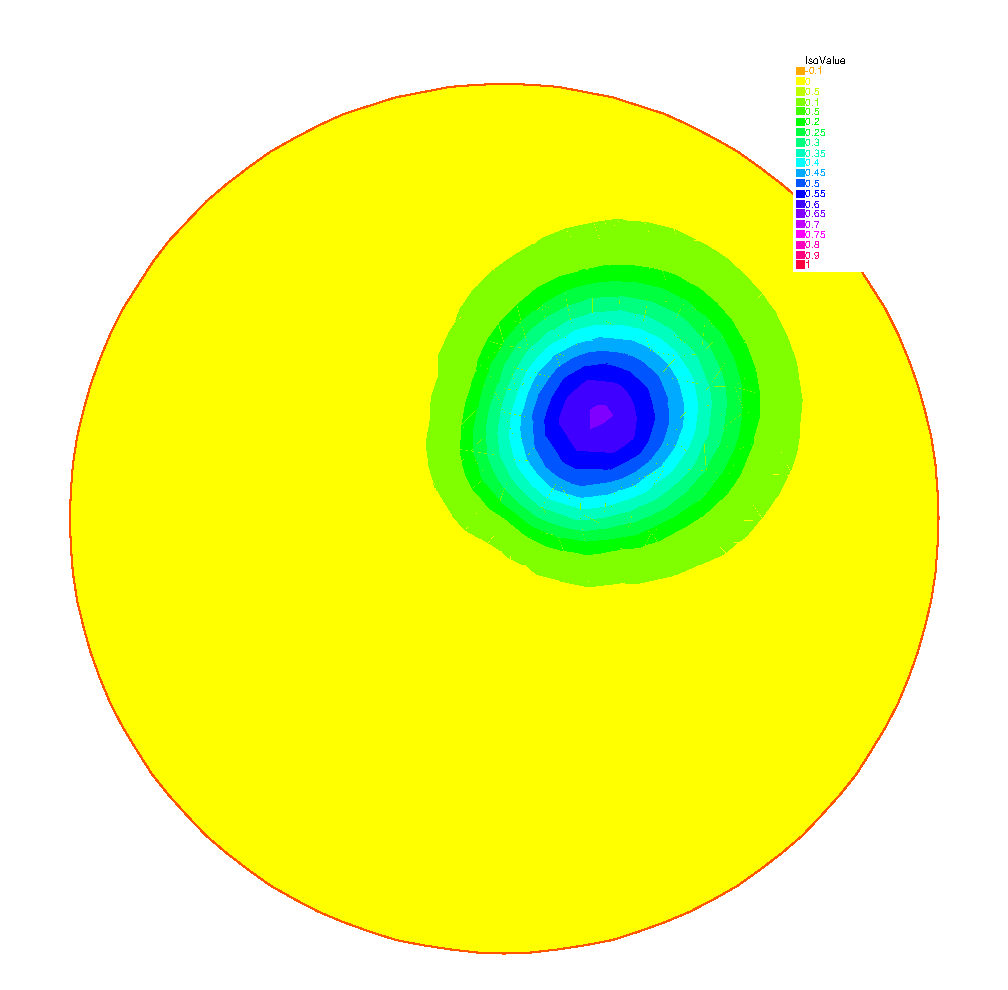
\includegraphics[width=8cm]{convectCG}
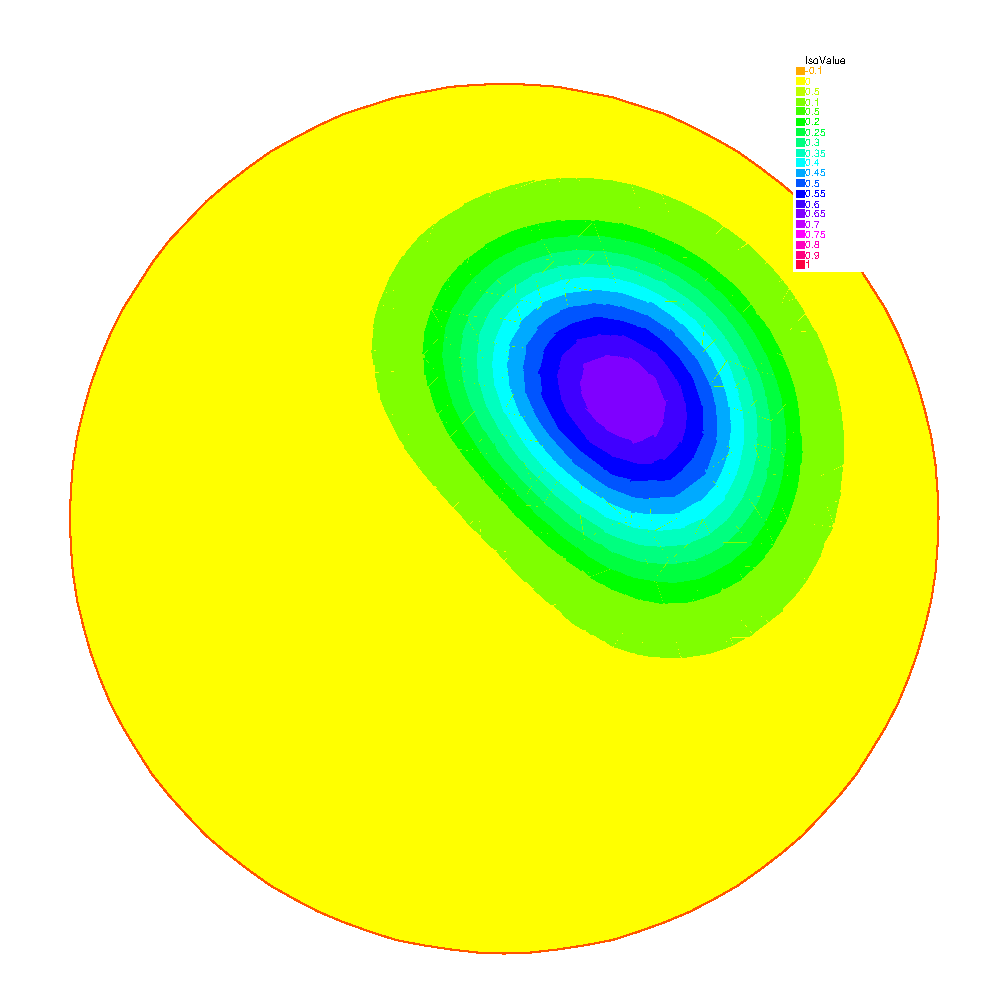
\includegraphics[width=8cm]{convectDG}

\caption{\label{figconvect} The rotated hill after one revolution, left with Characteristics-Galerkin,
on the right with Discontinuous $P_1$ Galerkin FEM.}
\end{center}
\end{figure}

Now if you think that DG is too slow try this
\bFF

// the same DG very much faster
@varf aadual(cc,w) = @int2d(Th)((cc/dt+(v1*@dx(cc)+v2*@dy(cc)))*w)
        + @intalledges(Th)((1-@nTonEdge)*w*(al*abs(n)-n/2)*@jump(cc));
@varf bbdual(ccold,w) =  - @int2d(Th)(ccold*w/dt);
@matrix  AA= aadual(Vh,Vh);
@matrix BB = bbdual(Vh,Vh);
@set (AA,init=t,solver=sparsesolver);
Vh rhs=0;
@for ( t=0; t< 2*pi ; t+=dt)
{
  ccold=cc;
  rhs[] = BB* ccold[];
  cc[] = AA^-1*rhs[];
  @plot(cc,fill=0,cmm="t="+t + ", min=" + cc[].min + ", max=" +  cc[].max);
};
\eFF
Notice the new keyword \x{set} to specify a solver in this framework; the modifier \x{init} is used
to tel the solver that the matrix has not changed (init=true), and the name parameter are the
same that in problem definition (see. \ref{def problem}) \index{set}\index{problem}.

\paragraph{\x{Finite Volume Methods}} can also be handled with \freefempp but it requires programming.
For instance the $P_0-P_1$ Finite Volume Method of Dervieux et al associates to each $P_0$
function $c^1$ a $P_0$ function $c^0$ with constant value around each vertex $q^i$ equal to $c^1(q^i)$
on the cell $\sigma_i$ made by all the medians of all triangles having $q^i$ as vertex.
Then upwinding is done by taking left or right values at the median:
\[
    \int_{\sigma_i}\frac 1{\delta t}({c^1}^{n+1}-{c^1}^n) + \int_{\p\sigma_i}u\cdot n c^-=0
    ~~~\forall i
\]
It can be programmed as
\bFF
@load "mat_dervieux";  // external module in C++ must be loaded
@border a(t=0, 2*pi){ x = cos(t); y = sin(t);  }
@mesh th = @buildmesh(a(100));
@fespace Vh(th,P1);

Vh vh,vold,u1 = y, u2 = -x;
Vh v = exp(-10*((x-0.3)^2 +(y-0.3)^2)), vWall=0, rhs =0;

@real dt = 0.025;
// qf1pTlump means mass lumping is used
@problem  FVM(v,vh) = @int2d(th,qft=qf1pTlump)(v*vh/dt)
                  - @int2d(th,qft=qf1pTlump)(vold*vh/dt)
      + @int1d(th,a)(((u1*N.x+u2*N.y)<0)*(u1*N.x+u2*N.y)*vWall*vh)
+ rhs[] ;

@matrix A;
MatUpWind0(A,th,vold,[u1,u2]);

@for ( @int t=0; t< 2*pi ; t+=dt){
  vold=v;
  rhs[] = A * vold[] ; FVM;
  @plot(v,wait=0);
};
\eFF
the \x{mass lumping} parameter forces a quadrature formula with Gauss points at the vertices
so as to make the mass matrix diagonal; the linear system solved by a conjugate gradient method for
instance will then converge in one or two iterations.

\index{MatUpWind0}
The right hand side {\tt rhs} is computed by an \x{external C++ function} {\tt MatUpWind0(...)}
which is programmed as
\bFF
// computes matrix a on a triangle for the Dervieux FVM
@int   fvmP1P0(@double q[3][2], // the 3 vertices of a triangle T
              @double u[2],   // convection velocity on T
              @double c[3],   // the P1 function on T
              @double a[3][3],// output matrix
              @double where[3] ) // where>0 means we're on the boundary
{
  @for(@int i=0;i<3;i++) @for(@int j=0;j<3;j++) a[i][j]=0;

    @for(@int i=0;i<3;i++){
        @int ip = (i+1)%3, ipp =(ip+1)%3;
        @double unL =-((q[ip][1]+q[i][1]-2*q[ipp][1])*u[0]
                    -(q[ip][0]+q[i][0]-2*q[ipp][0])*u[1])/6;
        @if(unL>0) { a[i][i] += unL; a[ip][i]-=unL;}
            @else{ a[i][ip] += unL; a[ip][ip]-=unL;}
        @if(where[i]&&where[ip]){        // this is a boundary edge
            unL=((q[ip][1]-q[i][1])*u[0] -(q[ip][0]-q[i][0])*u[1])/2;
            if(unL>0) { a[i][i]+=unL; a[ip][ip]+=unL;}
        }
    }
  return 1;
}
\eFF
It must be inserted into a larger .cpp file, shown in Appendix A,
 which is the load module linked to \freefempp.


 \subsection{The System of elasticity}

\paragraph{Elasticity}

Solid objects deform under the action of applied forces:
a point in the solid, originally at $(x,y,z)$ will come to $(X,Y,Z)$
after some time; the vector $\mathbf{u}=(u_1,u_2,u_3) = (X-x, Y-y, Z-z)$ is called
the displacement. When the displacement is small and the solid is
elastic, Hooke's law gives a relationship between the stress tensor
$\sigma(u)=(\sigma_{ij}(u) )$ and the strain tensor $\epsilon(u)=\epsilon_{ij}(u)$
$$
\sigma_{ij}(u) = \lambda \delta_{ij} \nabla.\mathbf{u}+ 2\mu\epsilon_{ij}(u),
$$
where the Kronecker symbol $\delta_{ij} = 1$ if $i=j$, $0$ otherwise, with
$$\epsilon_{ij}(u) = {1\over 2}({\p u_i\over\p x_j} +
{\p u_j\over\p x_i} ),
$$
and where $\lambda, \mu$ are two constants that describe the
mechanical properties of the solid, and are themselves related to the
better known constants $E$, Young's modulus, and $\nu$, Poisson's ratio:
$$ \mu = {E\over 2( 1+\nu)}, \quad \lambda = {E\nu\over (1+\nu)(1-2\nu)}.
$$


 \paragraph{Lam\'e's system}

Let us consider a beam with axis $Oz$ and with perpendicular section
$\Omega$. The components along $x$ and $y$ of the strain ${\bf u}(x)$
in a section $\Omega$ subject to forces ${\bf f}$ perpendicular to the
axis are governed by \\
$$
  -\mu \Delta {\bf u} - (\mu+\lambda)  \nabla (\nabla .{\bf u})={\bf f}~~\hbox{in}~~\Omega,
$$
 where $\lambda ,\mu  $ are the Lam\'{e} coefficients introduced above.

Remark, we do not used this equation because the associated  variationnal
form does not give the right boundary condition, we simply use
$$
  - div( \sigma ) = \mathbf{f}  \quad  \mbox{in} \Omega
$$
where the corresponding variationnal form is:
$$
 \int_{\Omega} \sigma(u) : \epsilon(\mathbf{v})\;dx - \int_{\Omega}  \mathbf{v} f \;dx =0;
$$
where $:$  denote the tensor scalar product,   i.e. $ a: b = \sum_{i,j}  a_{ij}b_{ij}$.

So the variationnal form can be written as :
$$
 \int_{\Omega} \lambda \nabla.u   \nabla.v  + 2 \mu \epsilon(\mathbf{u}):\epsilon(\mathbf{v}) \; dx - \int_{\Omega}  \mathbf{v} f  \;dx  =0;
$$
 \paragraph{Example}  Consider  elastic plate with the undeformed rectangle shape
$[0,20]\times [-1,1]$.
The body force is the gravity force $\vec f$ and the
boundary force $\vec g$ is zero on lower, upper and right sides.
 The left vertical sides of the beam is fixed.
 The boundary conditions are
\begin{eqnarray*}
     \sigma . {\bf n}  &=& g = 0    ~~\hbox{on}~~\Gamma_1, \Gamma_4, \Gamma_3, \\
      {\bf u} &=& \mathbf{0} ~~\hbox{on}~~\Gamma_2
 \end{eqnarray*}
Here ${\bf u}=(u,v) $ has two components.\bigskip

The above two equations are strongly coupled by their mixed
derivatives, and thus any iterative solution on each of the
components is risky. One should rather use \freefempp's system
approach and write:

\begin{example}[lame.edp]\label{lame.edp}
\bFF
// file lame.edp
@mesh Th=@square(10,10,[20*x,2*y-1]);
@fespace Vh(Th,P2);
Vh u,v,uu,vv;
@real sqrt2=sqrt(2.);
@macro epsilon(u1,u2)  [dx(u1),dy(u2),(dy(u1)+dx(u2))/sqrt2] // EOM  \index{macro!with parameter}
//the sqrt2 is because we want: epsilon(u1,u2)'* epsilon(v1,v2) $==  \epsilon(\bm{u}): \epsilon(\bm{v})$
@macro div(u,v) ( dx(u)+dy(v) ) // EOM


@real E = 21e5, nu = 0.28, mu= E/(2*(1+nu));
@real lambda = E*nu/((1+nu)*(1-2*nu)), f = -1; //

@solve lame([u,v],[uu,vv])= int2d(Th)(
        lambda*@div(u,v)*@div(uu,vv)
        +2.*mu*( @epsilon(u,v)'*@epsilon(uu,vv) ) )	
        - int2d(Th)(f*vv)
        + on(4,u=0,v=0);
@real coef=100;
@plot([u,v],wait=1,ps="lamevect.eps",coef=coef);

@mesh th1 = movemesh(Th, [x+u*coef, y+v*coef]);
@plot(th1,wait=1,ps="lamedeform.eps");
@real dxmin  = u[].min;
@real dymin  = v[].min;

@cout << " - dep.  max   x = "<< dxmin<< " y=" << dymin << endl;
@cout << "   dep.  (20,0)  = " << u(20,0) << " " << v(20,0) << endl;
\eFF
\end{example}

The numerical results are shown on figure \ref{figlame} and the output is:
\bFF
 -- square mesh : nb vertices  =121 ,  nb triangles = 200 ,  nb boundary edges 40
 -- Solve :           min -0.00174137  max 0.00174105
          min -0.0263154  max 1.47016e-29
 - dep.  max   x = -0.00174137 y=-0.0263154
   dep.  (20,0)  = -1.8096e-07 -0.0263154
times: compile 0.010219s, execution 1.5827s
\eFF



\begin{figure}[hbtp]
\begin{center}
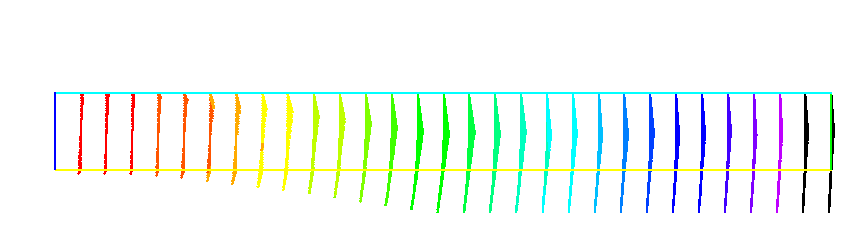
\includegraphics[width=15cm]{lamevect}\\
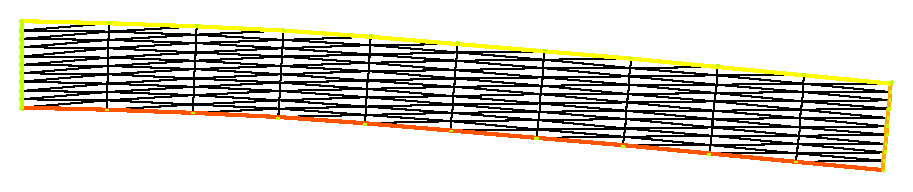
\includegraphics[width=15cm]{lamedeform}

\caption{\label{figlame} Solution of Lam\'e's equations for elasticity for a 2D beam deflected by its
own weight and clamped by its left vertical side; result are shown with a amplification factor equal to  100.
{\em Remark: the size of the arrow  is automatically bound, but the color gives the real length}}
\end{center}
\end{figure}

\subsection{The System of Stokes for Fluids}

In the case of a flow invariant with respect to the third coordinate
(two-dimensional flow), flows at low Reynolds number (for instance
micro-organisms) satisfy,
\begin{eqnarray*}&&
    \vec -\Delta u + \n p =0
    \cr&&
    \n\cdot \vec u =0
\end{eqnarray*}
where $\vec u=(u_1,u_2)$ is the fluid velocity and $p$ its pressure.
\\
The driven cavity is a standard test. It is a box full of liquid with its lid moving horizontally
at speed one.  The pressure and the velocity must be discretized in compatible fintie
element spaces for the LBB conditions to be satisfied:
\[
    \sup_{p\in P_h}\frac{(\vec u,\n p)}{|p|}\geq \beta|\vec u|~~~\forall \vec u\in U_h
\]
\bFF
//file stokes.edp
@int n=3;
@mesh Th=@square(10*n,10*n);
@fespace Uh(Th,P1b); Uh u,v,uu,vv;
@fespace Ph(Th,P1);  Ph p,pp;

@solve stokes([u,v,p],[uu,vv,pp]) =
    @int2d(Th)(@dx(u)*@dx(uu)+@dy(u)*@dy(uu) + @dx(v)*@dx(vv)+ @dy(v)*@dy(vv)
              + @dx(p)*uu + @dy(p)*vv + pp*(@dx(u)+@dy(v))
              -\bf 1e-10*p*pp\tt)
            + @on(1,2,4,u=0,v=0) + @on(3,u=1,v=0);
@plot([u,v],p,wait=1);
\eFF

Remark, we add a stabilization term {\bf{-10e-10*p*pp}} to fixe the constant part of the pressure.
\begin{figure}[htbp]
\begin{center}
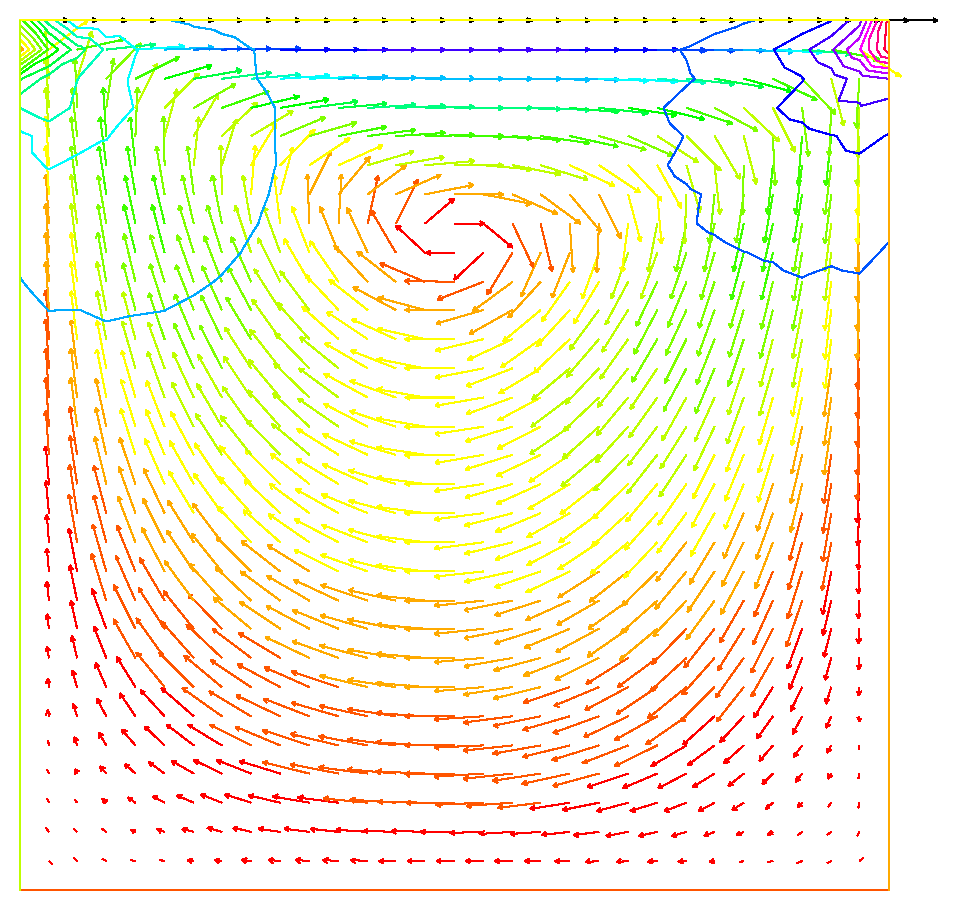
\includegraphics[width=8cm]{stokes}

\caption{\label{figstokes} Solution of Stokes' equations for the driven cavity problem, showing the
velocity field and the pressure level lines.}
\end{center}
\end{figure}

Results are shown on figure \ref{figstokes}

%\subsection{A Large Fluid Problem}
%A friend of one of us in Auroville-India was building a ramp to access an air conditioned room. As I was visiting the construction site he told me that he expected to cool air escaping by the door to the room to slide down the ramp and refrigerate the feet of the coming visitors.  I told him "no way" and decided to check numerically.  The results are on the front page of this book.
%\\
%The fluid velocity and pressure are solution of the Navier-Stokes equations with varying density function of the temperature.
%\\
%The geometry is trapezoidal with prescribed inflow made of cool air at the bottom and warm air above and so are the initial conditions; there is free outflow, slip velocity at the top (artificial) boundary and no-slip at the bottom.  However the Navier-Stokes cum temperature equations have a RANS $k-\epsilon$ model and a Boussinesq approximation for the buoyancy. This comes to
%\begin{eqnarray}&&
%\p_t\theta+u\n\theta-\n\cdot(\kappa_T^m\n\theta)=0
%\cr&&
%\p_t u +u\n u -\n\cdot(\mu_T\n u) +\n p+ e(\theta-\theta_0)\vec e_2,~~\n\cdot u=0
%\cr&&
%\mu_T = c_\mu\frac{k^2}\epsilon,~~\kappa_T=\kappa\mu_T
%\cr&&
%\p_t k + u\n k + \epsilon  -\n\cdot(\mu_T\n k)  = \frac{\mu_T}2|\n u+\n u^T|^2
%\cr&&
%\p_t\epsilon+u\n\epsilon + c_2\frac{\epsilon^2} k -\frac{c_\epsilon}{c_\mu}\n\dot(\mu_T\n\epsilon)= \frac{c_1}2  k|\n u+\n u^T|^2=0
%\end{eqnarray}
%We use a time discretization which preserves positivity and uses the method of characteristics ($X^m\approx x-u^m(x)\delta t$)
%\begin{eqnarray}&&
%\frac 1{\delta t}(\theta^{m+1}-\theta^m \circ X^m)-\n\cdot(\kappa_T^m\n\theta^{m+1})=0
%\cr&&
%\frac1{\delta t}(u^{m+1}-u^m \circ X^m) -\n\cdot(\mu_T^m\n u^{m+1}) +\n p^{m+1}+ e(\theta^{m+1}-\theta_0)\vec e_2
%,~~\n\cdot u^{m+1}=0
%\cr&&
%\frac1{\delta t}(k^{m+1}-k^m \circ X^m) + k^{m+1}\frac{\epsilon^m}{k^m}  -\n\cdot(\mu_T^m\n k^{m+1})  = \frac{\mu_T^m}2|\n u^m+{\n u^m}^T|^2
%\cr&&
%\frac1{\delta t}(\epsilon^{m+1}-\epsilon^m \circ X^m) + c_2\epsilon^{m+1}\frac{\epsilon^m} {k^m} -\frac{c_\epsilon}{c_\mu}\n\dot(\mu_T^m\n\epsilon^{m+1})= \frac{c_1}2  k^m|\n u^m+{\n u^m}^T|^2
%\cr&&
%\mu_T ^{m+1}= c_\mu\frac{{k^{m+1}}^2}{\epsilon^{m+1}},~~\kappa_T^{m+1}=\kappa\mu_T^{m+1}
%\end{eqnarray}
%In variational form and with appropriated boundary conditions the problem is:

%\bFF
%@real L=6;
%@border aa(t=0,1){x=t; y=0 ;}
%@border bb(t=0,14){x=1+t; y= - 0.1*t ;}
%@border cc(t=-1.4,L){x=15; y=t ;}
%@border dd(t=15,0){x= t ; y = L;}
%@border ee(t=L,0.5){ x=0; y=t ;}
%@border ff(t=0.5,0){ x=0; y=t ;}
%@int n=8;
%@mesh Th=@buildmesh(aa(n)+bb(9*n) + cc(4*n) + dd(10*n)+ee(6*n) + ff(n));
%@real s0=clock();

%@fespace Vh2(Th,P1b); // velocity space
%@fespace Vh(Th,P1); // pressure space
%@fespace V0h(Th,P0); // for gradients
%Vh2 u2,v2,up1=0,up2=0;
%Vh2 u1,v1;
%Vh  u1x=0,u1y,u2x,u2y, vv;

%@real reylnods=500;
%//cout << " Enter the reynolds number :"; cin >> reylnods;
%assert(reylnods>1 && reylnods < 100000);
%up1=0;
%up2=0;
%@func g=(x)*(1-x)*4;  // inflow
%Vh p=0,q, temp1,temp=35, k=0.001,k1,ep=0.0001,ep1;
%V0h muT=1,prodk,prode, kappa=0.25e-4, stress;
%@real alpha=0, eee=9.81/303;
%@real  nu=1, numu=nu/sqrt(0.09), nuep=pow(nu,1.5)/4.1;
%@int i=0,iter=0;
%@real dt=0;
%@problem TEMPER(temp,q) = // temperature equation
%   @ int2d(Th)(
%             alpha*temp*q + kappa * ( dx(temp)*dx(q) + dy(temp)*dy(q) ))
%//   + @int1d(Th,aa,bb)(temp*q*0.1)
%  +@ int2d(Th) ( -alpha*convect([up1,up2],-dt,temp1)*q )
%   + @on(ff,temp=25)
%  + @on(aa,bb,temp=35) ;

%@problem kine(k,q)=  // get the kinetic turbulent energy
%    @int2d(Th)(
%             (ep1/k1+alpha)*k*q + muT * ( dx(k)*dx(q) + dy(k)*dy(q) ))
%//   + int1d(Th,aa,bb)(temp*q*0.1)
%  + @int2d(Th) ( prodk*q-alpha*convect([up1,up2],-dt,k1)*q )
%   + @on(ff,k=0.0001)  + @on(aa,bb,k=numu*stress) ;

% @problem viscturb(ep,q)= // get the rate of turbulent viscous energy
%    @int2d(Th)(
%             (1.92*ep1/k1+alpha)*ep*q + muT * ( dx(ep)*dx(q) + dy(ep)*dy(q) ))
%//   +@ int1d(Th,aa,bb)(temp*q*0.1)
%  + @int2d(Th) ( prode*q-alpha*convect([up1,up2],-dt,ep1)*q )
%   + @on(ff,ep=0.0001) + @on(aa,bb,ep=nuep*pow(stress,1.5)) ;
%
%
% @solve NS ([u1,u2,p],[v1,v2,q]) = // Navier-Stokes k-epsilon and Boussinesq
%    @int2d(Th)(
%             alpha*( u1*v1 + u2*v2)
%            + muT * (dx(u1)*dx(v1)+dy(u1)*dy(v1)+dx(u2)*dx(v2)+dy(u2)*dy(v2))
% //           ( 2*dx(u1)*dx(v1) + 2*dy(u2)*dy(v2)+(dy(u1)+dx(u2))*(dy(v1)+dx(v2)))
%            + p*q*(0.000001)
%            - p*dx(v1) - p*dy(v2)
%            - dx(u1)*q - dy(u2)*q
%           )
%  + @int1d(Th,aa,bb,dd)(u1*v1*0.1)
%  +@ int2d(Th) (eee*(temp-35)*v1 -alpha*convect([up1,up2],-dt,up1)*v1
%                             -alpha*convect([up1,up2],-dt,up2)*v2 )
%   + @on(ff,u1=3,u2=0)
%  + @on(ee,u1=0,u2=0)
%  +@ on(aa,dd,u2=0)
%  + @on(bb,u2= -up1*N.x/N.y)
%  + @on(cc,u2=0) ;
% @plot(coef=0.2,cmm=" [u1,u2] et p  ",p,[u1,u2],ps="StokesP2P1.eps",value=1,wait=1);
%{
%  @real[int] xx(21),yy(21),pp(21);
%  @for (@int i=0;i<21;i++)
%   {
%     yy[i]=i/20.;
%     xx[i]=u1(0.5,i/20.);
%     pp[i]=p(i/20.,0.999);
%    }
%      @cout << " " << yy << endl;
%//     plot([xx,yy],wait=1,cmm="u1 x=0.5 cup");
%//     plot([yy,pp],wait=1,cmm="pressure y=0.999 cup");
%}

%dt = 0.05;
%@int nbiter = 3;
%@real coefdt = 0.25^(1./nbiter);
%@real coefcut = 0.25^(1./nbiter) , cut=0.01;
%@real tol=0.5,coeftol = 0.5^(1./nbiter);
%nu=1./reylnods;

%@for (iter=1;iter<=nbiter;iter++)
%{
% @cout << " dt = " << dt << " ------------------------ " << endl;
%  alpha=1/dt;
% @ for (i=0;i<=500;i++)
%   {
%     up1=u1;
%     up2=u2;
%     temp1=max(temp,25);
%     temp1=min(temp1,35);
%     k1=k; ep1=ep;
%     muT=0.09*k*k/ep;
%      NS; @plot([u1,u2],wait=1); // Solves Navier-Stokes
%     prode =0.126*k*(pow(2*dx(u1),2)+pow(2*dy(u2),2)+2*pow(dx(u2)+dy(u1),2))/2;
%     prodk= prode*k/ep*0.09/0.126;
%     kappa=muT/0.41;
%     stress=abs(dy(u1));
%     kine; @plot(k,wait=1);
%     viscturb; @plot(ep,wait=1);
%     TEMPER; // solves temperature equation
%     @if ( !(i % 5)){
%     	@plot(temp,value=1,fill=true,ps="temp_"+iter+"_"+i+".ps");
%     	@plot(coef=0.2,cmm=" [u1,u2] et p  ",p,[u1,u2],ps="plotNS_"+iter+"_"+i+".ps");
% 	}
%     @cout << "CPU " << clock()-s0 << "s " << endl;
%   }
%
%  @if (iter>= nbiter) @break;
%   Th=@adaptmesh(Th,[dx(u1),dy(u1),dx(u1),dy(u2)],splitpbedge=1,
%   			abserror=0,cutoff=cut,err=tol, inquire=0,ratio=1.5,hmin=1./1000);
% @plot(Th,ps="ThNS.eps");
%  dt = dt*coefdt;
%  tol = tol *coeftol;
%  cut = cut *coefcut;
%}
%@cout << "CPU " <<@clock()-s0 << "s " << endl;
%\eFF

\subsection{A Projection Algorithm for the Navier-Stokes equations }
\paragraph{Summary}\emph{Fluid flows require good algorithms and good triangultions. We show
here an example of a complex algorithm and or first example of \x{mesh adaptation}}.
\\\\
An incompressible viscous fluid satisfies:
$$ \p _t u + u\cdot\nabla u + \nabla p - \nu\Delta u = 0,\quad  \nabla\cdot u=0
\quad  \hbox{ in } \Omega\times ]0,T[,
$$
$$ u|_{t=0} = u^0,\quad  u|_\Gamma = u_\Gamma.
$$
A possible algorithm, proposed by Chorin, is
$$ {1\over \delta t}[u^{m+1} - u^moX^m] + \nabla p^m -\nu\Delta u^m= 0,\quad  u|_\Gamma
 = u_\Gamma,
 $$
$$ -\Delta p^{m+1} = -\nabla\cdot  u^moX^m, \quad  \p _n p^{m+1} = 0,
$$
where $uoX(x) = u(x-u(x)\delta t)$ since $\p _t u + u\cdot\nabla
u $ is approximated by the method of characteristics, as in the previous section.
\\\\
An improvement over Chorin's algorithm, given by Rannacher, is to compute a correction, q,
to the pressure (the overline denotes the mean over $\Omega$)
\[
    -\Delta q= \n\cdot\vec u - \overline{\n\cdot\vec u}
\]
and define
\[
    u^{m+1}=\tilde u + \n q\delta t,~~~p^{m+1}=p^m-q-\overline{p^m-q}
\]
where $\tilde u$ is the $(u^{m+1},v^{m+1})$ of Chorin's algorithm.

\paragraph{The backward facing step}

The geometry is that of a channel with a backward facing step so that
the inflow section is smaller than the outflow section. This geometry
produces a fluid recirculation zone that must be captured correctly.

This can only be done if the triangulation is sufficiently fine, or
well adapted to the flow.

Remark (FH), The are a technical difficulty is the example, the discret flow flux must be 
$0$ and in the previous version this is not the case, the correction is not so simple. 

\begin{example}[NSprojection.edp]\index{adaptmesh}\index{mesh!adaptation}
\bFF
// file NSprojection.edp

@border a0(t=1,0){ x=0;      y=t;      label=1;}
@border a1(t=0,1){ x=2*t;    y=0;        label=2;}
@border a2(t=0,1){ x=2;      y=-t/2;       label=2;}
@border a3(t=0,1){ x=2+18*t^1.2;  y=-0.5;       label=2;}
@border a4(t=0,1){ x=20;     y=-0.5+1.5*t;   label=3;}
@border a5(t=1,0){ x=20*t; y=1;        label=4;}
@int n=1;
@mesh Th= buildmesh(a0(3*n)+a1(20*n)+a2(10*n)+a3(150*n)+a4(5*n)+a5(100*n));
plot(Th);
@fespace Vh(Th,P1);
@real nu = 0.0025, dt = 0.2; // Reynolds=200
@func uBCin =  4*y*(1-y)*(y>0)*(x<2) ; 
@func uBCout =  4./1.5*(y+0.5)*(1-y) *(x>19);
Vh w,u = uBCin, v =0, p = 0, q=0;
@real area= int2d(Th)(1.);
Vh ubc  = uBCin + uBCout; 
@real influx0  = int1d(Th,1) (ubc*N.x), // FH add
      outflux0 = int1d(Th,3) (ubc*N.x); // FH add
verbosity=1;
@for(@int n=0;n<300;n++){
	
  Vh uold = u,  vold = v, pold=p;
  Vh f=convect([uold,vold],-dt,uold); 
  @real outflux = int1d(Th,3) (f*N.x); // FH add
  f = f - (influx0+outflux)/outflux0 * uBCout; // FH add
  outflux = int1d(Th,3) (f*N.x); // FH add
  assert( abs(influx0+outflux) < 1e-10); // WARNING the flux must be 0 ..
  
  @solve pb4u(u,w,init=n,solver=LU)
        =int2d(Th)(u*w/dt +nu*(dx(u)*dx(w)+dy(u)*dy(w)))
        -int2d(Th)((convect([uold,vold],-dt,uold)/dt-dx(p))*w)
        + on(1,u = 4*y*(1-y)) + on(2,4,u = 0) + on(3,u=f);
  plot(u);

  @solve pb4v(v,w,init=n,solver=LU)
        = int2d(Th)(v*w/dt +nu*(dx(v)*dx(w)+dy(v)*dy(w)))
        -int2d(Th)((convect([uold,vold],-dt,vold)/dt-dy(p))*w)
        +on(1,2,3,4,v = 0);

 @real meandiv = int2d(Th)(dx(u)+dy(v))/area;

 @solve pb4p(q,w,init=n,solver=LU)= int2d(Th)(dx(q)*dx(w)+dy(q)*dy(w))
    - int2d(Th)((dx(u)+ dy(v)-meandiv)*w/dt)+ on(3,q=0);

 @real meanpq = int2d(Th)(pold - q)/area;
 if(n%50==49){
    Th = adaptmesh(Th,[u,v],q,err=0.04,nbvx=100000);
    plot(Th, wait=true);
    ubc = uBCin + uBCout; // reinterpolate B.C. 
    influx0 = int1d(Th,1) (ubc*N.x); // FH add
    outflux0 = int1d(Th,3) (ubc*N.x); // FH add
 }
 p = pold-q-meanpq;
 u = u + dx(q)*dt;
 v = v + dy(q)*dt;
 real err = sqrt(int2d(Th)(square(u-uold)+square(v-vold))/Th.area) ;
 cout << " iter " << n << " Err L2 = " << err << endl;
 if(err < 1e-3) break;
}
plot(p,wait=1,ps="NSprojP.eps");
plot(u,wait=1,ps="NSprojU.eps");\eFF
\end{example}

\begin{figure}[htbp]
\begin{center}

\includegraphics[width=15cm]{NSprojTh}\\
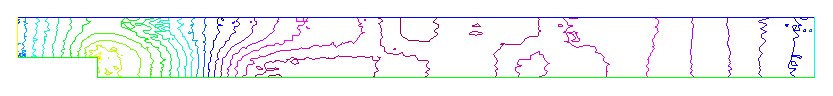
\includegraphics[width=15cm]{NSprojP}\\
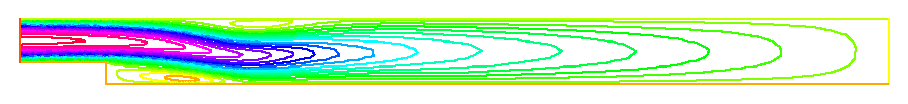
\includegraphics[width=15cm]{NSprojU}

\caption{\label{figNSproj} Rannacher's projection algorithm: result on an adapted mesh (top) showing
the pressure (middle) and the horizontal velocity $u$ at Reynolds 400.}
\end{center}
\end{figure}

We show in figure \ref{figNSproj} the numerical results obtained for a Reynolds
number of 400 where mesh adaptation is done after 50 iterations on the first mesh.

\subsection{Newton Method for the Steady Navier-Stokes equations}

The problem is find the velocity field $\bm{u}=(u_i)_{i=1}^d$ and the pressure $p$ of a Flow 
satisfying in the domain $\Omega \subset  \mathbb{R}^d (d=2,3)$:
\Blue{\begin{eqnarray*}
 (\bm{u}\cdot\nabla) \bm{u}-\nu \Delta \bm{u}+\nabla p&=&0,\\ \nabla\cdot \bm{u}&=&0
\end{eqnarray*}}
where $\nu$ is the viscosity of the fluid, $\nabla = (\p_i )_{i=1}^d $, the dot product is $\cdot$, and  $\Delta = \nabla\cdot\nabla$
with the some boundary conditions ( $\bm{u}$ is  given on $\Gamma$)

\bigskip

The weak form is 
find $\bm{u}, p $ such than for $\forall \bm{v}$ (zero on $\Gamma$), and $\forall  q$ 
\Blue{\begin{equation}
  \int_\Omega  ((\bm{u}\cdot\nabla) \bm{u} ). \bm v + \nu \nabla \bm{u}:\nabla \bm{v} 
  - p \nabla\cdot \bm{v} - q \nabla\cdot \bm{u} = 0 
\end{equation}}


The Newton Algorithm to solve nonlinear Problem is

Find  $u\in  V$ such that $F(u)=0$ where 
$ F : V \mapsto V $. 

\begin{enumerate} \index{Newton Algorithm
}
\item choose $u_0\in \R^n $ , ;
\item for ( $i =0$; $i$ < niter; $i = i+1$) 

\begin{enumerate}
\item solve $DF(u_i) w_i =  F(u_i)$;
\item $u_{i+1} = u_i - w_i$;  
\end{enumerate}
 break  $|| w_i|| < \varepsilon$.
\end{enumerate}

Where $DF(u)$ is the differential of $F$ at point  $u$, this is a linear application such that:
{$
  F(u+\delta) = F(u) + DF(u) \delta + o(\delta) 
$}


For Navier Stokes, $F$ and $DF$ are  :
\Blue{\small
\begin{eqnarray*}F(\bm{u},p) =  \int_\Omega  &&((\bm{u}\cdot\nabla) \bm{u} ). \bm v + \nu \nabla \bm{u}:\nabla \bm{v} 
  - p \nabla\cdot \bm{v} - q \nabla\cdot \bm{u}\\
DF(\bm{u},p)(\bm{\delta u} ,\delta p)  =  \int_\Omega  &&((\bm{\delta u}\cdot\nabla) \bm{u} ). \bm v + ((\bm{u}\cdot\nabla) \bm{\delta u} ). \bm v \\
 &+& \nu \nabla \bm{\delta u}:\nabla \bm{v}  - \delta p \nabla\cdot \bm{v} - q \nabla\cdot \bm{\delta u}
\end{eqnarray*}}



So the Newton algorithm become   
\begin{example}[NSNewton.edp] 
\bFF
...   
	@for( n=0;n< 15;n++)
	{ @solve Oseen([du1,du2,dp],[v1,v2,q]) =
          @int2d(Th) (  nu*(Grad(du1,du2)'*Grad(v1,v2) )
                      + UgradV(du1,du2, u1, u2)'*[v1,v2]
                      + UgradV( u1, u2,du1,du2)'*[v1,v2]
                      - div(du1,du2)*q - div(v1,v2)*dp 
                      - 1e-8*dp*q // stabilization term 
                     )
        - @int2d(Th) (  nu*(Grad(u1,u2)'*Grad(v1,v2) )
                      + UgradV(u1,u2, u1, u2)'*[v1,v2]
                      - div(u1,u2)*q - div(v1,v2)*p 
                     )
        + @on(1,du1=0,du2=0) ;
      u1[] -= du1[];  u2[] -= du2[]; p[]  -= dp[];
      err= du1[].linfty + du2[].linfty + dp[].linfty;        
      @if(err < eps) @break;    
      @if( n>3 && err > 10.) @break; //  blowup ???? 
    }
\eFF


With the  operator: 
\bFF
@macro Grad(u1,u2) [ dx(u1),dy(u1) , dx(u2),dy(u2) ]// 
@macro UgradV(u1,u2,v1,v2) [ [u1,u2]'*[dx(v1),dy(v1)] ,
                            [u1,u2]'*[dx(v2),dy(v2)] ]// 
@macro div(u1,u2)  (dx(u1)+dy(u2))//
\eFF

We build a computation mesh the exterior of a 2d cylinder. 

\bFF
@real R = 5,L=15;
@border cc(t=0,2*pi){ x=cos(t)/2;y=sin(t)/2;label=1;}
@border ce(t=pi/2,3*pi/2) { x=cos(t)*R;y=sin(t)*R;label=1;}
@border beb(tt=0,1) { real t=tt^1.2; x= t*L; y= -R; label = 1;}
@border beu(tt=1,0) { real t=tt^1.2; x= t*L; y= R; label = 1;}
@border beo(t=-R,R) {  x= L; y= t; label = 0;}
@border bei(t=-R/4,R/4) {  x= L/2; y= t; label = 0;}
@mesh Th=buildmesh(cc(-50)+ce(30)+beb(20)+beu(20)+beo(10)+bei(10));
@plot(Th);

// bounding box for the plot
@func bb=[[-1,-2],[4,2]];

/  FE Space Taylor Hood
@fespace Xh(Th,P2);// for volicity 
@fespace Mh(Th,P1);// for pressure 
Xh u1,u2,v1,v2,du1,du2,u1p,u2p;
Mh p,q,dp,pp;

// intial guess with B.C. 
u1 = ( x^2+y^2) > 2;
u2=0;
\eFF

Finally we use  trick to make continuation on the viscosity $\nu$, because the Newton method blowup 
owe start with the final viscosity $\nu$
\bFF
//  Physical parameter
real nu= 1./50, nufinal=1/200. ,cnu=0.5;

// stop test for Newton
real eps=1e-6;

verbosity=0;
while(1)  //  Loop on viscosity
{   int n;
    real err=0; // err on Newton algo ... 
    
      ... put the new the Newton  algo here
        
	if(err < eps)                                                               
	 { // converge decrease $\nu$ (more difficult)                                                                                                                           
	   plot([u1,u2],p,wait=1,cmm=" rey = " + 1./nu , coef=0.3,bb=bb);                                                           
	   @if( nu == nufinal) break;                                                                                                
	   @if( n < 4) cnu=cnu^1.5; // fast converge => change faster                                                                
	   nu = max(nufinal, nu* cnu); // new vicosity                                                                              
	   u1p=u1;  u2p=u2;  pp=p; //  save correct solution ...                                                                    
	 }                                                                                                                          
	 @else 
	 {   //  blowup increase $\nu$  (more simple)                                                                         
	   @assert(cnu< 0.95); //  the method  finally  blowup                                                                                               
	   nu = nu/cnu; //  get previous value of viscosity                                                                         
	   cnu= cnu^(1./1.5); // no conv. => change lower                                                                           
	   nu = nu* cnu;  // new viscosity                                                                                           
	   cout << " restart nu = " << nu << " Rey= "<< 1./nu << "  (cnu = " << cnu << " ) \n";                                     
	   // restore a correct solution ..                                                                                           
	   u1=u1p;                                                                                                                  
	   u2=u2p;                                                                                                                  
	   p=pp;                                                                                                                    
	 }     
}        
\eFF
\end{example}

\begin{figure}[htbp]
\begin{center}
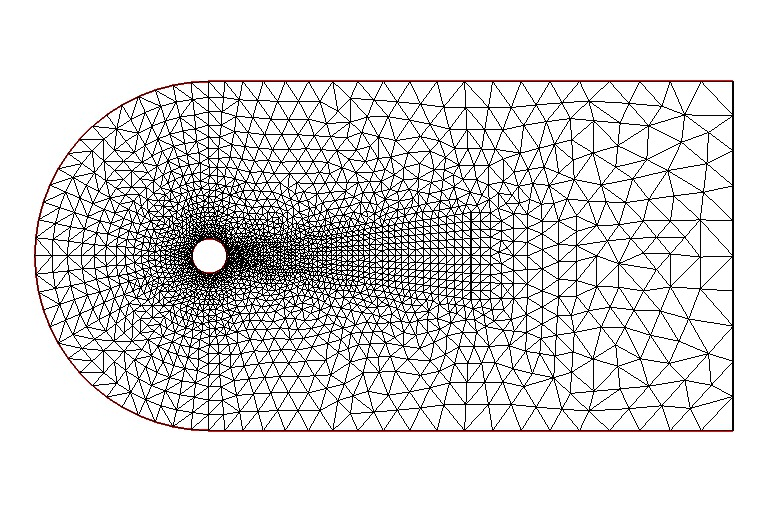
\includegraphics[width=8cm]{NSNewtonTh}
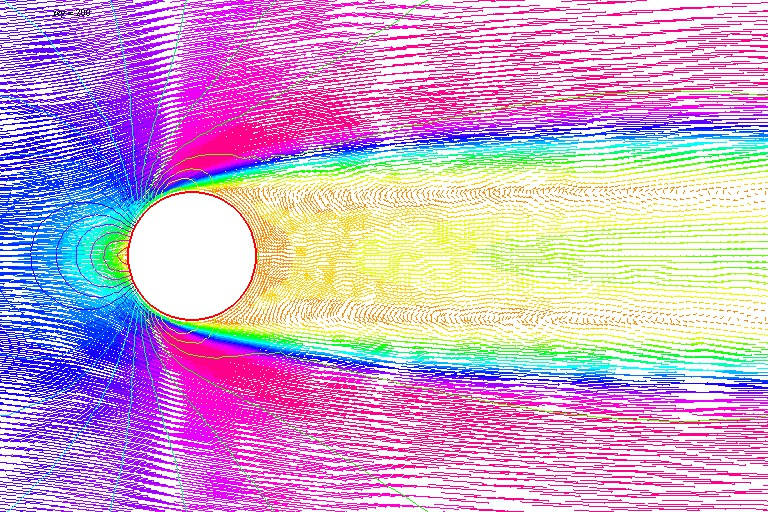
\includegraphics[width=8cm]{NSNewtonUP}
\caption{\label{NSNewton} Mesh and the velocity and pressure at Reynolds  $ 200$ }
\end{center}
\end{figure}


%\paragraph{Gag's or Bug with Stokes Equation, with Boundary condition}
%
%
%Denote: \Blue{$\Gamma$} the boundary, \Blue{$\bm{n}$} the unit exterior normal,  
%\Blue{$\varepsilon(\bm{u}) =  ( ^t \nabla \bm{u}+ \nabla \bm{u})/2 $}, \Blue{$I_d$} the Identity matrix.
%
%\begin{enumerate}
%\item With BC, the incompressibility imply
%\Red{$ \int_\Gamma \bm{u}.\bm{n} =0 $} at discrete level. 
%\item 
% The force in the fluid on surface $\Sigma$ is \Blue{$ \int_\Sigma (\nu\; \varepsilon(\bm{u})  -  p I_d) \bm{n}  $}. The Weak form is  
%$\forall \bm{v}, q$ :
%\[  \int_\Omega  \nu \nabla \bm{u}:\nabla \bm{v} 
%  - p \nabla\cdot \bm{v} - q \nabla\cdot \bm{u} = {\int_\Gamma \;{}^t\bm{n}(\nu \nabla \bm{u} -  p I_d )   \bm{v} }
%  \]
%    Or with a more physical formulation (with the true strain $\varepsilon$):
%\[  \int_\Omega  \nu\; \varepsilon( \bm{u}):\varepsilon( \bm{v}) 
%  - p \nabla\cdot \bm{v} - q \nabla\cdot \bm{u} = {\int_\Gamma \;{}^t\bm{n}(\nu \varepsilon (\bm{u}) -  p I_d )   \bm{v} }
%  \]  
%\end{enumerate}
%
%\begin{figure}[htbp]
%\begin{center}
%\includegraphics[width=8cm]{NSnewtonU}
%\includegraphics[width=8cm]{NSnewtonE}
%
%\caption{\label{figconvect} The rotated hill after one revolution, left with Characteristics-Galerkin,
%on the right with Discontinuous $P_1$ Galerkin FEM.}
%\end{center}
%\end{figure}
%



\subsection{A Large Fluid Problem}
A friend of one of us in Auroville-India was building a ramp to access an air conditioned room. As I was visiting the construction site he told me that he expected to cool air escaping by the door to the room to slide down the ramp and refrigerate the feet of the coming visitors.  I told him "no way" and decided to check numerically.  The results are on the front page of this book.
\\
The fluid velocity and pressure are solution of the Navier-Stokes equations with varying density function of the temperature.
\\
The geometry is trapezoidal with prescribed inflow made of cool air at the bottom and warm air above and so are the initial conditions; there is free outflow, slip velocity at the top (artificial) boundary and no-slip at the bottom.  However the Navier-Stokes cum temperature equations have a RANS $k-\epsilon$ model and a Boussinesq approximation for the buoyancy. This comes to
\begin{eqnarray}&&
\p_t\theta+u\n\theta-\n\cdot(\kappa_T^m\n\theta)=0
\cr&&
\p_t u +u\n u -\n\cdot(\mu_T\n u) +\n p+ e(\theta-\theta_0)\vec e_2,~~\n\cdot u=0
\cr&&
\mu_T = c_\mu\frac{k^2}\epsilon,~~\kappa_T=\kappa\mu_T
\cr&&
\p_t k + u\n k + \epsilon  -\n\cdot(\mu_T\n k)  = \frac{\mu_T}2|\n u+\n u^T|^2
\cr&&
\p_t\epsilon+u\n\epsilon + c_2\frac{\epsilon^2} k -\frac{c_\epsilon}{c_\mu}\n\cdot (\mu_T\n\epsilon)= \frac{c_1}2  k|\n u+\n u^T|^2=0
\end{eqnarray}
We use a time discretization which preserves positivity and uses the method of characteristics ($X^m(x)\approx  x-u^m(x)\delta t$)
\begin{eqnarray}&&
\frac 1{\delta t}(\theta^{m+1}-\theta^m \circ X^m)-\n\cdot(\kappa_T^m\n\theta^{m+1})=0
\cr&&
\frac1{\delta t}(u^{m+1}-u^m \circ X^m) -\n\cdot(\mu_T^m\n u^{m+1}) +\n p^{m+1}+ e(\theta^{m+1}-\theta_0)\vec e_2
,~~\n\cdot u^{m+1}=0
\cr&&
\frac1{\delta t}(k^{m+1}-k^m \circ X^m) + k^{m+1}\frac{\epsilon^m}{k^m}  -\n\cdot(\mu_T^m\n k^{m+1})  = \frac{\mu_T^m}2|\n u^m+{\n u^m}^T|^2
\cr&&
\frac1{\delta t}(\epsilon^{m+1}-\epsilon^m \circ X^m) + c_2\epsilon^{m+1}\frac{\epsilon^m} {k^m} -\frac{c_\epsilon}{c_\mu}\n\dot(\mu_T^m\n\epsilon^{m+1})= \frac{c_1}2  k^m|\n u^m+{\n u^m}^T|^2
\cr&&
\mu_T ^{m+1}= c_\mu\frac{{k^{m+1}}^2}{\epsilon^{m+1}},~~\kappa_T^{m+1}=\kappa\mu_T^{m+1}
\end{eqnarray}
In variational form and with appropriated boundary conditions the problem is:

\bFF
@real L=6;
@border aa(t=0,1){x=t; y=0 ;}
@border bb(t=0,14){x=1+t; y= - 0.1*t ;}
@border cc(t=-1.4,L){x=15; y=t ;}
@border dd(t=15,0){x= t ; y = L;}
@border ee(t=L,0.5){ x=0; y=t ;}
@border ff(t=0.5,0){ x=0; y=t ;}
@int n=8;
@mesh Th=@buildmesh(aa(n)+bb(9*n) + cc(4*n) + dd(10*n)+ee(6*n) + ff(n));
@real s0=clock();

@fespace Vh2(Th,P1b); // velocity space
@fespace Vh(Th,P1); // pressure space
@fespace V0h(Th,P0); // for gradients
Vh2 u2,v2,up1=0,up2=0;
Vh2 u1,v1;
Vh  u1x=0,u1y,u2x,u2y, vv;

@real reylnods=500;
//cout << " Enter the reynolds number :"; cin >> reylnods;
assert(reylnods>1 && reylnods < 100000);
up1=0;
up2=0;
@func g=(x)*(1-x)*4;  // inflow
Vh p=0,q, temp1,temp=35, k=0.001,k1,ep=0.0001,ep1;
V0h muT=1,prodk,prode, kappa=0.25e-4, stress;
@real alpha=0, eee=9.81/303, c1m = 1.3/0.09 ;
@real  nu=1, numu=nu/sqrt( 0.09), nuep=pow(nu,1.5)/4.1;
@int i=0,iter=0;
@real dt=0;
@problem TEMPER(temp,q) = // temperature equation
   @ int2d(Th)(
             alpha*temp*q + kappa * ( dx(temp)*dx(q) + dy(temp)*dy(q) ))
//   + @int1d(Th,aa,bb)(temp*q* 0.1)
  +@ int2d(Th) ( -alpha*convect([up1,up2],-dt,temp1)*q )
   + @on(ff,temp=25)
  + @on(aa,bb,temp=35) ;

@problem kine(k,q)=  // get the kinetic turbulent energy
    @int2d(Th)(
             (ep1/k1+alpha)*k*q + muT * ( dx(k)*dx(q) + dy(k)*dy(q) ))
//   + int1d(Th,aa,bb)(temp*q*0.1)
  + @int2d(Th) ( prodk*q-alpha*convect([up1,up2],-dt,k1)*q )
   + @on(ff,k=0.0001)  + @on(aa,bb,k=numu*stress) ;

 @problem viscturb(ep,q)= // get the rate of turbulent viscous energy
    @int2d(Th)(
             (1.92*ep1/k1+alpha)*ep*q + c1m*muT * ( dx(ep)*dx(q) + dy(ep)*dy(q) ))
//   +@ int1d(Th,aa,bb)(temp*q*0.1)
  + @int2d(Th) ( prode*q-alpha*convect([up1,up2],-dt,ep1)*q )
   + @on(ff,ep= 0.0001) + @on(aa,bb,ep=nuep*pow(stress,1.5)) ;


 @solve NS ([u1,u2,p],[v1,v2,q]) = // Navier-Stokes k-epsilon and Boussinesq
    @int2d(Th)(
             alpha*( u1*v1 + u2*v2)
            + muT * (dx(u1)*dx(v1)+dy(u1)*dy(v1)+dx(u2)*dx(v2)+dy(u2)*dy(v2))
 //           ( 2*dx(u1)*dx(v1) + 2*dy(u2)*dy(v2)+(dy(u1)+dx(u2))*(dy(v1)+dx(v2)))
            + p*q*(0.000001)
            - p*dx(v1) - p*dy(v2)
            - dx(u1)*q - dy(u2)*q
           )
  + @int1d(Th,aa,bb,dd)(u1*v1* 0.1)
  +@ int2d(Th) (eee*(temp-35)*v1 -alpha*convect([up1,up2],-dt,up1)*v1
                             -alpha*convect([up1,up2],-dt,up2)*v2 )
   + @on(ff,u1=3,u2=0)
  + @on(ee,u1=0,u2=0)
  +@ on(aa,dd,u2=0)
  + @on(bb,u2= -up1*N.x/N.y)
  + @on(cc,u2=0) ;
 @plot(coef=0.2,cmm=" [u1,u2] et p  ",p,[u1,u2],ps="StokesP2P1.eps",value=1,wait=1);
{
  @real[int] xx(21),yy(21),pp(21);
  @for (@int i=0;i<21;i++)
   {
     yy[i]=i/20.;
     xx[i]=u1(0.5,i/20.);
     pp[i]=p(i/20.,0.999);
    }
      @cout << " " << yy << endl;
//     plot([xx,yy],wait=1,cmm="u1 x=0.5 cup");
//     plot([yy,pp],wait=1,cmm="pressure y=0.999 cup");
}

dt = 0.05;
@int nbiter = 3;
@real coefdt = 0.25^(1./nbiter);
@real coefcut = 0.25^(1./nbiter) , cut=0.01;
@real tol=0.5,coeftol = 0.5^(1./nbiter);
nu=1./reylnods;

@for (iter=1;iter<=nbiter;iter++)
{
 @cout << " dt = " << dt << " ------------------------ " << endl;
  alpha=1/dt;
 @ for (i=0;i<=500;i++)
   {
     up1=u1;
     up2=u2;
     temp1=max(temp,25);
     temp1=min(temp1,35);
     k1=k; ep1=ep;
     muT=0.09*k*k/ep;
      NS; @plot([u1,u2],wait=1); // Solves Navier-Stokes
     prode =0.126*k*(pow(2*dx(u1),2)+pow(2*dy(u2),2)+2*pow(dx(u2)+dy(u1),2))/2;
     prodk= prode*k/ep*0.09/0.126;
     kappa=muT/0.41;
     stress=abs(dy(u1));
     kine; @plot(k,wait=1);
     viscturb; @plot(ep,wait=1);
     TEMPER; // solves temperature equation
     @if ( !(i % 5)){
         @plot(temp,value=1,fill=true,ps="temp_"+iter+"_"+i+".ps");
         @plot(coef=0.2,cmm=" [u1,u2] et p  ",p,[u1,u2],ps="plotNS_"+iter+"_"+i+".ps");
     }
     @cout << "CPU " << clock()-s0 << "s " << endl;
   }

  @if (iter>= nbiter) @break;
   Th=@adaptmesh(Th,[dx(u1),dy(u1),dx(u1),dy(u2)],splitpbedge=1,
               abserror=0,cutoff=cut,err=tol, inquire=0,ratio=1.5,hmin=1./1000);
 @plot(Th,ps="ThNS.eps");
  dt = dt*coefdt;
  tol = tol *coeftol;
  cut = cut *coefcut;
}
@cout << "CPU " <<@clock()-s0 << "s " << endl;
\eFF


\subsection{An Example with Complex Numbers}

 \index{FE function!complex}\index{complex}\index{Helmholtz}
In a microwave oven heat comes from molecular excitation by an
electromagnetic field. For a plane monochromatic wave, amplitude is
given by Helmholtz's equation:
$$ \beta v + \Delta v = 0.
$$
We consider a rectangular oven where the wave is emitted by part of
the upper wall. So the boundary of the domain is made up of a part
$\Gamma_1$ where $v=0$ and of another part $\Gamma_2=[c,d]$ where for
instance $v=\sin(\pi{y-c\over c-d})$.

Within an object to be cooked, denoted by $B$, the heat source is
proportional to $v^2$.
At equilibrium, one has

$$-\Delta\theta = v^2 I_B, \quad \theta_\Gamma = 0
$$
where $I_B$ is $1$ in the object and $0$ elsewhere.
\begin{figure}[htbp]
\begin{center}
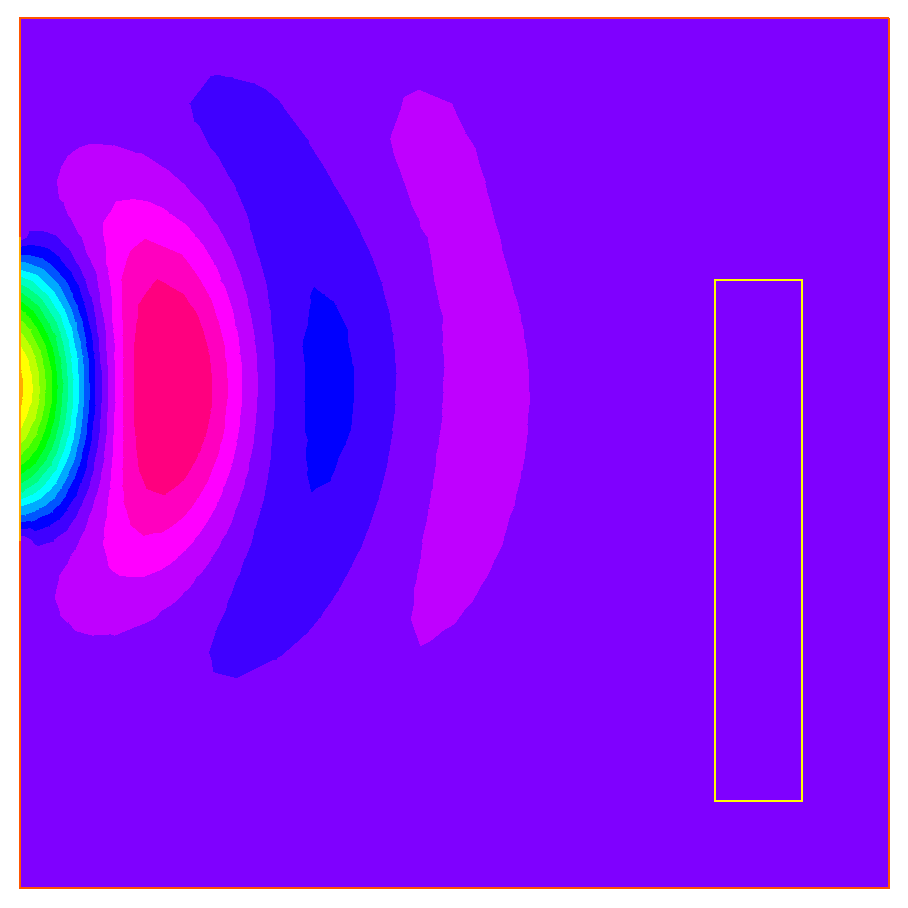
\includegraphics[width=5cm]{rmuonde}
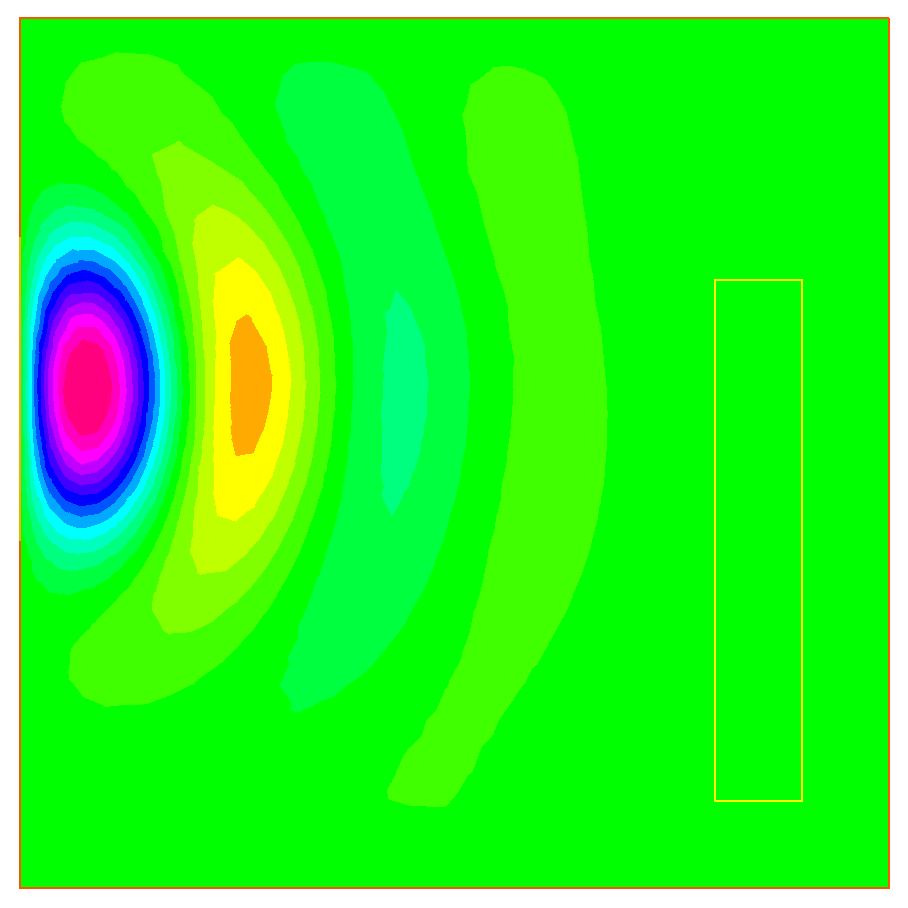
\includegraphics[width=5cm]{imuonde}
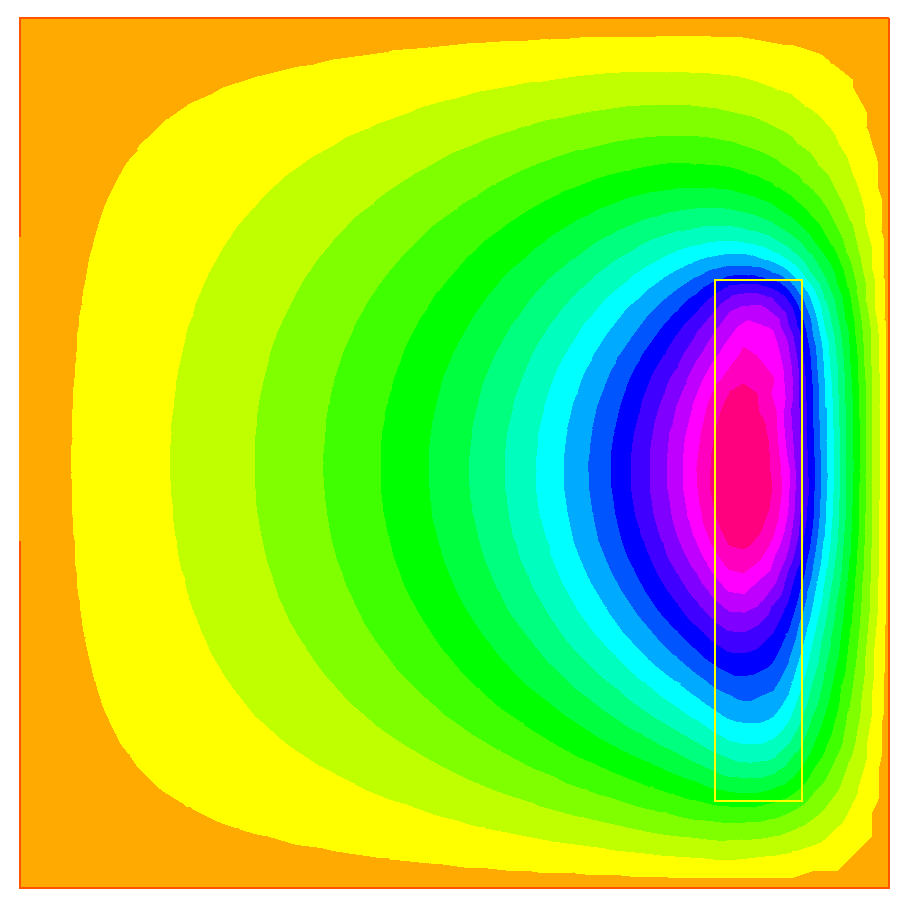
\includegraphics[width=5cm]{tempmuonde}
\caption{\label{figmuonde}A microwave oven: real (left) and imaginary (middle) parts
 of wave  and temperature (right).}
\end{center}
\end{figure}

Results are shown on figure \ref{figmuonde}

In the program below $\beta = 1/(1-I/2)$ in the air and $2/(1-I/2)$
in the object ($i=\sqrt{-1}$):

\begin{example}[muwave.edp]
\bFF

// file muwave.edp
@real a=20, b=20, c=15, d=8, e=2, l=12, f=2, g=2;
@border a0(t=0,1) {x=a*t; y=0;label=1;}
@border a1(t=1,2) {x=a; y= b*(t-1);label=1;}
@border a2(t=2,3) { x=a*(3-t);y=b;label=1;}
@border a3(t=3,4){x=0;y=b-(b-c)*(t-3);label=1;}
@border a4(t=4,5){x=0;y=c-(c-d)*(t-4);label=2;}
@border a5(t=5,6){ x=0; y= d*(6-t);label=1;}

@border b0(t=0,1) {x=a-f+e*(t-1);y=g; label=3;}
@border b1(t=1,4) {x=a-f; y=g+l*(t-1)/3; label=3;}
@border b2(t=4,5) {x=a-f-e*(t-4); y=l+g; label=3;}
@border b3(t=5,8) {x=a-e-f; y= l+g-l*(t-5)/3; label=3;}
@int n=2;
@mesh Th = @buildmesh(a0(10*n)+a1(10*n)+a2(10*n)+a3(10*n)
        +a4(10*n)+a5(10*n)+b0(5*n)+b1(10*n)+b2(5*n)+b3(10*n));
@plot(Th,wait=1);
@fespace Vh(Th,P1);
@real meat =  Th(a-f-e/2,g+l/2).@region, air= Th(0.01,0.01).@region;
Vh R=(region-air)/(meat-air);

Vh<@complex> v,w;
@solve muwave(v,w) = @int2d(Th)(v*w*(1+R)
                -(@dx(v)*@dx(w)+@dy(v)*@dy(w))*(1-0.5i))
   + @on(1,v=0) + @on(2, v=sin(pi*(y-c)/(c-d)));
Vh vr=@real(v), vi=@imag(v);
@plot(vr,wait=1,ps="rmuonde.ps", fill=true);
@plot(vi,wait=1,ps="imuonde.ps", fill=true);

@fespace Uh(Th,P1); Uh u,uu, ff=1e5*(vr^2 + vi^2)*R;

@solve temperature(u,uu)= @int2d(Th)(@dx(u)* @dx(uu)+ @dy(u)* @dy(uu))
     - @int2d(Th)(ff*uu) + @on(1,2,u=0);
@plot(u,wait=1,ps="tempmuonde.ps", fill=true);
\eFF
\end{example}

\subsection{Optimal Control} Thanks to the function \texttt{BFGS} it
is possible to solve complex nonlinear optimization problem within
\texttt{FreeFem++}. For example consider the following inverse
problem
\[
    \min_{b,c,d\in R}J=\int_E(u-u_d)^2~:~
    -\nabla(\kappa(b,c,d)\cdot\nabla u)=0,~~u|_\Gamma=u_\Gamma
\]
where the desired state $u_d$, the boundary data $u_\Gamma$ and the
observation set $E\subset\Omega$ are all given.  Furthermore let us
assume that
\[
    \kappa(x)=1+bI_B(x)+cI_C(x)+dI_D(x)~~~\forall x\in\Omega
\]
where $B,C,D$ are separated subsets of $\Omega$.
\\\\
To solve this problem by the quasi-Newton BFGS method we need the
derivatives of $J$ with respect to $b,c,d$.  We self explanatory
notations, if $\delta b,\delta c,\delta d$ are variations of
$b,c,d$ we have
\[
    \delta J\approx 2\int_E(u-u_d)\delta u,~~
    -\nabla(\kappa\cdot\nabla\delta u)\approx\nabla(\delta\kappa\cdot\nabla
    u)
    ~~\delta u|_\Gamma=0
\]
Obviously $J'_b$ is equal to $\delta J$ when $\delta b=1,\delta
c=0,\delta d=0$, and so on for $J'_c$ and $J'_d$.
\\\\
All this is implemented in the following program
 \bFF
// file optimcontrol.edp
@border aa(t=0, 2*pi) {    x = 5*cos(t);    y = 5*sin(t);  };
@border bb(t=0, 2*pi) {    x = cos(t);    y = sin(t);  };
@border cc(t=0, 2*pi) {    x = -3+cos(t);    y = sin(t);  };
@border dd(t=0, 2*pi) {    x = cos(t);    y = -3+sin(t);  };
@mesh th = @buildmesh(aa(70)+bb(35)+cc(35)+dd(35));
@fespace Vh(th,P1);
Vh Ib=((x^2+y^2)<1.0001),
   Ic=(((x+3)^2+ y^2)<1.0001),
   Id=((x^2+(y+3)^2)<1.0001),
   Ie=(((x-1)^2+ y^2)<=4),
   ud,u,uh,du;
@real[int] z(3);
@problem A(u,uh) =@int2d(th)((1+z[0]*Ib+z[1]*Ic+z[2]*Id)*(dx(u)*dx(uh)
                    +dy(u)*dy(uh))) + on(aa,u=x^3-y^3);
z[0]=2; z[1]=3; z[2]=4;
A; ud=u;
@ofstream f("J.txt");
@func @real J(real[int] & Z)
{
    @for (int i=0;i<z.n;i++)z[i]=Z[i];
    A; @real s= @int2d(th)(Ie*(u-ud)^2);
    f<<s<<"   "; @return s;
}

@real[int] dz(3), dJdz(3);

@problem B(du,uh)
  =@int2d(th)((1+z[0]*Ib+z[1]*Ic+z[2]*Id)*(dx(du)*dx(uh)+dy(du)*dy(uh)))
  +@int2d(th)((dz[0]*Ib+dz[1]*Ic+dz[2]*Id)*(dx(u)*dx(uh)+dy(u)*dy(uh)))
  +@on(aa,du=0);

@func @real[int] DJ(@real[@int] &Z)
    {
      @for(int i=0;i<z.n;i++)
        { @for(int j=0;j<dz.n;j++) dz[j]=0;
          dz[i]=1; B;
          dJdz[i]= 2*int2d(th)(Ie*(u-ud)*du);
      }
     @return dJdz;
 }

 @real[@int] Z(3);
 @for(@int j=0;j<z.n;j++) Z[j]=1;
 BFGS(J,DJ,Z,eps=1.e-6,nbiter=15,nbiterline=20);
 @cout << "BFGS: J(z) = " << J(Z) <<  endl;
 @for(int j=0;j<z.n;j++) cout<<z[j]<<endl;
 @plot(ud,value=1,ps="u.eps");
\eFF
In this example the sets $B,C,D,E$ are circles of boundaries $bb,cc,dd,ee$ are the domain
$\Omega$ is the circle of boundary $aa$.  The desired state $u_d$ is the solution
of the PDE for $b=2,c=3,d=4$.  The unknowns are packed into array $z$.  Notice that it is
necessary to recopy $Z$ into $z$ because one is a local variable while the other one is global.
The program found $b=2.00125,c=3.00109,d=4.00551$.
Figure \ref{figcontrol} shows $u$ at convergence
and the successive function evaluations of $J$.
\begin{figure}[htbp]
\begin{center}
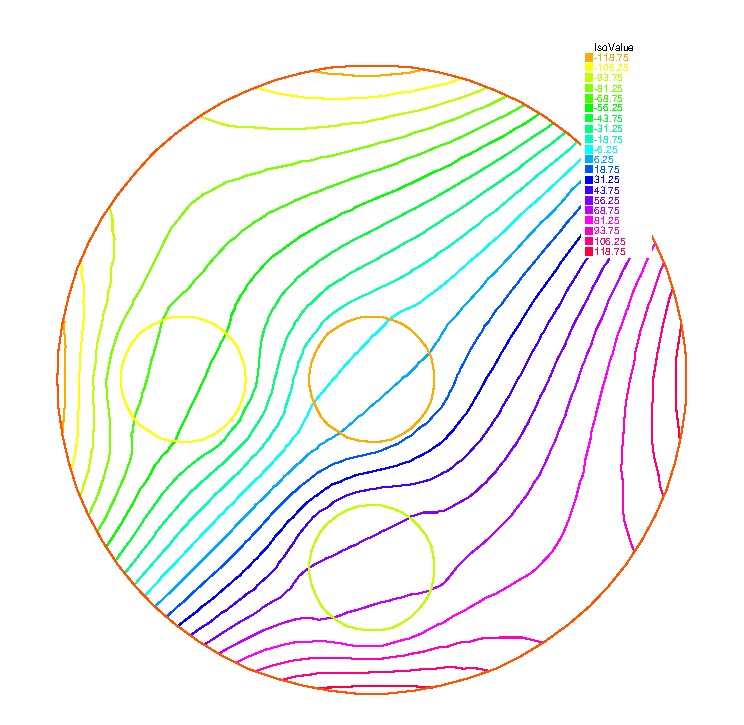
\includegraphics[width=5cm]{u-bfgs}
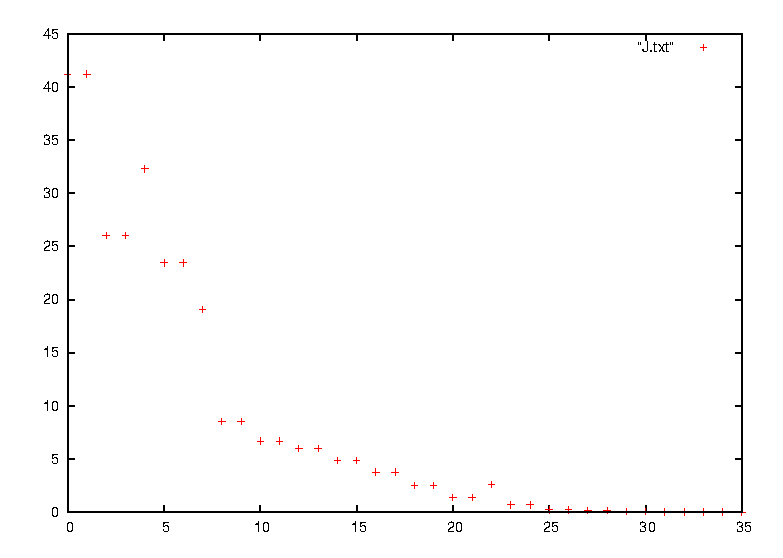
\includegraphics[width=5cm]{J-bfgs}
\caption{\label{figcontrol}On the left the level lines of $u$. On the right the successive evaluations of
$J$ by BFGS (5 values above 500 have been removed for readability)}
\end{center}
\end{figure}
Note that an \emph{adjoint state} could have been used. Define $p$ by
\[
-\nabla\cdot(\kappa\nabla p)=2I_E(u-u_d),~~~p|_\Gamma=0
\]
Consequently
\begin{eqnarray}&&
\delta J = -\int_{\Omega} (\nabla\cdot(\kappa\nabla p))\delta u
\cr&&
= \int_\Omega(\kappa\nabla p\cdot\nabla\delta u)
=-\int_\Omega(\delta\kappa\nabla p\cdot\nabla u)
\end{eqnarray}
Then the derivatives are found by setting $\delta b=1, \delta c=\delta d=0$ and so on:
\[
    J'_b=-\int_B \nabla p\cdot\nabla u,~~J'_c=-\int_C \nabla p\cdot\nabla u,~~
    J'_d=-\int_D \nabla p\cdot\nabla u
\]
\paragraph{Remark} As BFGS stores an $M\times M$ matrix where $M$ is the number of
unknowns, it is dangerously expensive to use this method when the unknown $x$ is a
Finite Element Function.  One should use another optimizer such as
the NonLinear Conjugate Gradient \texttt{NLCG} (also a key word
of \texttt{FreeFem++}).  See the file algo.edp in the examples folder.

\subsection{A Flow with Shocks}
Compressible Euler  equations should be discretized with Finite Volumes or FEM with flux up-winding scheme but these are not implemented in \freefempp.  Nevertheless acceptable results can be obtained with the method of characteristics
provided that the mean values $\bar f=\frac12(f^++f^-)$ are used at shocks in the scheme, and finally  mesh adaptation \index{adaptmesh}\index{mesh!adaptation}.%
\begin{eqnarray}\label{euler}&&
    \p_t\rho+\bar u\n\rho + \bar\rho\n\cdot u=0
    \cr&&
   \bar\rho( \p_t u+\frac{\overline{\rho u}}{\bar\rho}\n u +\n p=0
    \cr&&
    \p_t p + \bar u\n p +(\gamma-1)\bar p\n\cdot u =0
\end{eqnarray}
%
One possibility is to couple $u,p$ and then update $\rho$, i.e.
%
\begin{eqnarray}\label{eulalgo}&&
    \frac 1{(\gamma-1)\delta t\bar p^m} (p^{m+1}-p^m \circ X^m) + \n\cdot u^{m+1} =0
    \cr&&
    \frac{\bar\rho^m}{\delta t}(u^{m+1}-u^m \circ {\tilde X}^m ) +\n p^{m+1}=0
    \cr&&
    \rho^{m+1} = \rho^m \circ X^m +
        \frac{\bar\rho^m}{(\gamma-1)\bar p^m}(p^{m+1}-p^m \circ X^m)
\end{eqnarray}
A numerical result is given on Figure \ref{figvfive} and the \freefempp script is

%
\begin{figure}[htbp]
\begin{center}
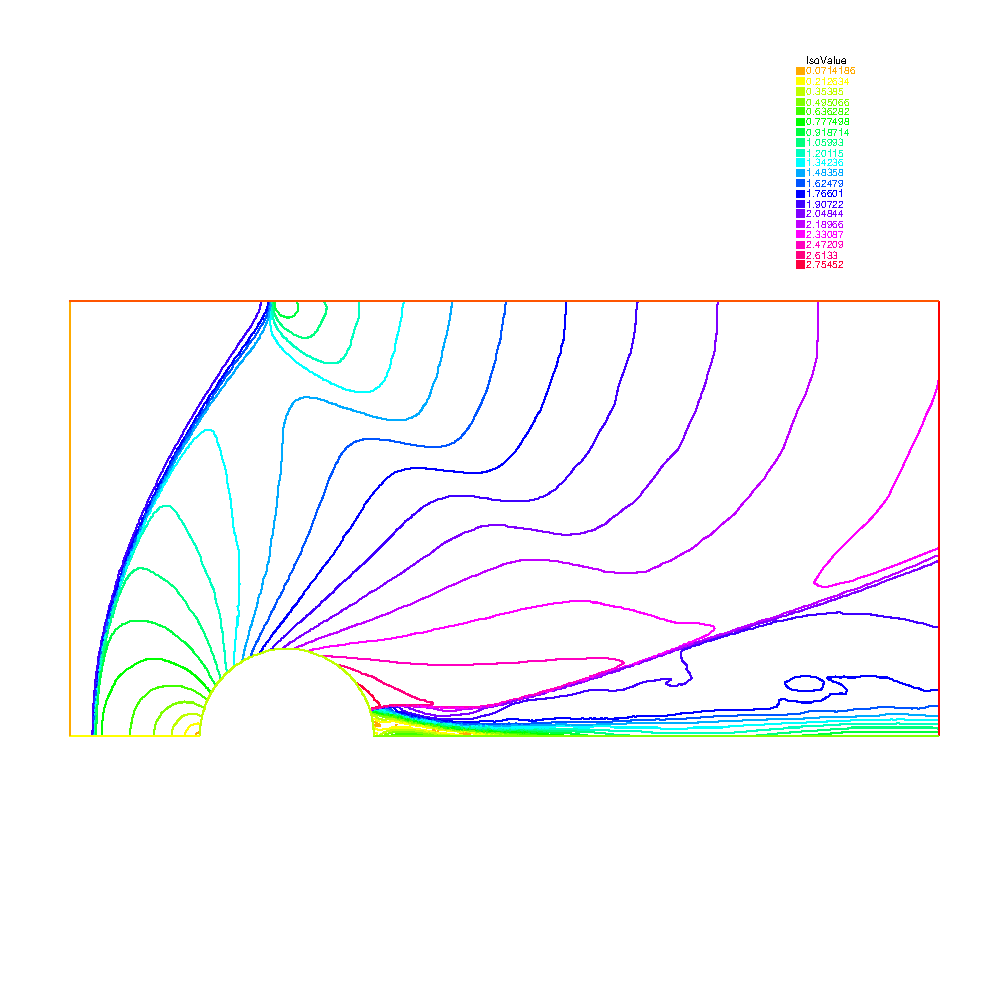
\includegraphics[width=10cm]{mach2r}
\caption{ \label{figvfive} Pressure for a Euler flow around a disk at Mach 2 computed by (\ref{eulalgo}) }
\end{center}
\end{figure}
%
\bFF
verbosity=1;
@int anew=1;
@real x0=0.5,y0=0, rr=0.2;
@border ccc(t=0,2){x=2-t;y=1;};
@border ddd(t=0,1){x=0;y=1-t;};
@border aaa1(t=0,x0-rr){x=t;y=0;};
@border cercle(t=pi,0){ x=x0+rr*cos(t);y=y0+rr*sin(t);}
@border aaa2(t=x0+rr,2){x=t;y=0;};
@border bbb(t=0,1){x=2;y=t;};

@int m=5; mesh Th;
@if(anew) Th = @buildmesh (ccc(5*m) +ddd(3*m) + aaa1(2*m) + cercle(5*m)
              + aaa2(5*m) + bbb(2*m) );
      @else Th = @readmesh("Th_circle.mesh"); plot(Th,wait=0);

@real dt=0.01, u0=2, err0=0.00625, pena=2;
@fespace Wh(Th,P1);
@fespace Vh(Th,P1);
Wh u,v,u1,v1,uh,vh;
Vh r,rh,r1;
@macro dn(u) (N.x*dx(u)+N.y*dy(u) ) //  def the normal derivative

@if(anew){ u1= u0; v1= 0; r1 = 1;}
@else {
    @ifstream g("u.txt");g>>u1[];
    @ifstream gg("v.txt");gg>>v1[];
    @ifstream ggg("r.txt");ggg>>r1[];
    @plot(u1,ps="eta.eps", value=1,wait=1);
    err0=err0/10; dt = dt/10;
}

@problem  eul(u,v,r,uh,vh,rh)
   = @int2d(Th)(  (u*uh+v*vh+r*rh)/dt
                  + ((dx(r)*uh+ dy(r)*vh) - (dx(rh)*u + dy(rh)*v))
               )
 + @int2d(Th)(-(rh*convect([u1,v1],-dt,r1) + uh*convect([u1,v1],-dt,u1)
                + vh*convect([u1,v1],-dt,v1))/dt)
  +@int1d(Th,6)(rh*u)   // +int1d(Th,1)(rh*v)
 + @on(2,r=0) + @on(2,u=u0) + @on(2,v=0);

@int j=80;
@for(int k=0;k<3;k++)
{
    @if(k==20){ err0=err0/10; dt = dt/10; j=5;}
    @for(@int i=0;i<j;i++){
       eul; u1=u; v1=v; r1=abs(r);
        @cout<<"k="<<k<<"  E="<<int2d(Th)(u^2+v^2+r)<<endl;
        @plot(r,wait=0,value=1);
}
Th = @adaptmesh (Th,r, nbvx=40000,err=err0,
      abserror=1,nbjacoby=2, omega=1.8,ratio=1.8, nbsmooth=3,
      splitpbedge=1, maxsubdiv=5,rescaling=1) ;
 @plot(Th,wait=0);
 u=u;v=v;r=r;

@savemesh(Th,"Th_circle.mesh");
@ofstream f("u.txt");f<<u[];
@ofstream ff("v.txt");ff<<v[];
@ofstream fff("r.txt");fff<<r[];
r1 = sqrt(u*u+v*v);
@plot(r1,ps="mach.eps", value=1);
r1=r;
}
\eFF

 \subsection{Classification of the equations}
\paragraph{Summary}\emph{
It is usually not easy to determine the type of a system.  Yet the approximations
and algorithms suited to the problem depend on its type:
\begin{itemize}
\item Finite Elements compatible (LBB conditions) for elliptic systems
\item Finite difference on the parabolic variable and a time loop on each
elliptic subsystem of parabolic systems; better stability diagrams when the schemes are implicit in time.
\item Upwinding, Petrov-Galerkin, Characteristics-Galerkin, Discontinuous-Galerkin, Finite Volumes
for hyperbolic systems plus, possibly, a time loop.
\end{itemize}
When the system changes type, then expect difficulties (like shock discontinuities)!}

 \paragraph{Elliptic, parabolic and hyperbolic equations}

A partial differential equation (PDE) is a relation between a function
of several variables and its derivatives.
 $$
 F(\varphi(x),{\p\varphi\over\p
 x_1}(x),\cdots,{\p\varphi\over\p
 x_d}(x),{\p^2\varphi\over\p
 x^2_1}(x),\cdots,{\p^m\varphi\over\p x^m_d}(x)) =
 0\quad\forall x\in\Omega\subset \Rel^d.
 $$
 The range of $x$ over which the equation is taken, here $\Omega$, is called
 the \emph{domain} of the PDE.
The highest derivation index, here $m$, is called the {\it
 order}. If $F$ and $\varphi$ are vector valued functions, then the
 PDE is actually a \emph{system} of PDEs.
 \\
Unless indicated otherwise, here by convention \emph{one} PDE
 corresponds to one scalar valued $F$ and $\varphi$.
If $F$ is linear with respect to its arguments, then the PDE is said
 to be \emph{linear}.
 \\
The general form of a second order, linear scalar PDE is
${\p^2\varphi\over\p x_i\p x_j}$ and $A:B$ means
 $\sum^d_{i,j=1} a_{ij} b_{ij}.$
 $$\alpha\varphi + a\cdot\nabla\varphi + B :\nabla(\nabla\varphi) =
 f{\quad\hbox{ in }\quad}\Omega\subset \Rel^d,
 $$
 where $f(x),\alpha(x)\in \Rel,
 a(x)\in \Rel^d, B(x)\in \Rel^{d\times d}$
are the PDE \emph{coefficients}.
If the coefficients are independent of $x$, the PDE is said to have
 \emph{constant coefficients}.

To a PDE we associate a quadratic form, by replacing
$\varphi$ by $1$,
 $\p\varphi/\p x_i$ by $z_i$ and
 $\p^2\varphi/\p x_i\p x_j$ by $z_i z_j$, where $z$
 is a vector in $\Rel^d$~:
 $$\alpha + a\cdot z + z^T Bz = f.
 $$
If it is the equation of an ellipse (ellipsoid if $d \geq 2$),
the PDE is said to be {\it elliptic};
if it is the equation of a parabola or a hyperbola, the PDE is said to
be {\it parabolic} or {\it hyperbolic}. If $A \equiv 0$, the degree is
no longer 2 but 1, and for reasons that will appear more clearly
later, the PDE is still said to be hyperbolic.
\\\\
These concepts can be generalized to systems, by studying whether or
not the polynomial system $P(z)$ associated with the PDE system has
branches at infinity (ellipsoids have no branches at infinity,
paraboloids have one, and hyperboloids have several).
\\
If the PDE is not linear, it is said to be \emph{non linear}.
Those are said to be locally elliptic, parabolic, or hyperbolic
according to the type of the linearized equation.
\\
For example, for the non linear equation
 $${\p^2\varphi\over\p t^2} - {\p\varphi\over\p
 x}{\p^2\varphi\over\p x^2} = 1,
 $$
  we have $d=2, x_1 = t, x_2 = x$ and its linearized form is:
 $${\p^2 u\over\p t^2} - {\p u\over\p x}
 {\p^2\varphi\over\p x^2} - {\p\varphi\over\p
 x}{\p^2 u\over\p x^2} = 0,
 $$
which for the unknown $u$ is locally elliptic if
 ${\p\varphi\over\p x} < 0$  and locally hyperbolic if
 ${\p\varphi\over\p x} > 0$.

\paragraph{Examples}

 \noindent{Laplace's} equation is elliptic:
 $$\Delta\varphi \equiv {\p^2\varphi\over\p x^2_1} +
 {\p^2\varphi\over\p x^2_2} + \cdots +
 {\p^2\varphi\over\p x^2_d} = f, \ \ \ \forall x
 \in \Omega\subset \Rel^d.
 $$
The \emph{heat} equation is parabolic in
 $Q = \Omega\times]0,T[\subset \Rel^{d+1}$~:
 $${\p\varphi\over\p t} - \mu\Delta\varphi = f\quad\forall
 x\in\Omega\subset  \Rel^d, \quad\forall t\in]0,T[.
 $$
If $\mu >0$,  the \emph{wave} equation is hyperbolic:
 $${\p^2\varphi\over\p t^2} - \mu\Delta\varphi =
 f{\quad\hbox{~in~}\quad}  Q.
 $$
The \emph{convection diffusion} equation is parabolic if $\mu \neq 0$
 and hyperbolic otherwise:
 $${\p\varphi\over\p t} + a\nabla\varphi -
 \mu\Delta\varphi = f.
 $$
The \emph{biharmonic} equation is elliptic:
 $$\Delta(\Delta\varphi) = f{\quad\hbox{~in~}\quad}\Omega.
 $$

\paragraph{Boundary conditions}

A relation between a function and its derivatives is not sufficient to define the function.
Additional information on the boundary $\Gamma=\p\Omega$ of
$\Omega$, or on part of $\Gamma$ is necessary.\\
Such information is called a \emph{boundary condition}.
For example,
 $$\varphi(x) \ \hbox{given},\ \forall x\in \Gamma,
 $$
is called a \emph{\x{Dirichlet} boundary condition}.
The \emph{\x{Neumann}} condition is
 $${\p\varphi\over\p n}(x) \ \hbox{given on }\
 \Gamma \hbox{~~~(or~~} n\cdot B\nabla\varphi,\hbox{given on }\
 \Gamma\hbox{ for a general second order PDE)}
$$
  where $n$ is the normal at $x\in\Gamma$
directed towards the exterior of $\Omega$ (by definition
 ${\p\varphi\over\p n}=\nabla\varphi\cdot n$).

Another classical condition, called a \emph{Robin} (or \emph{Fourier})
condition is written as:
 $$\varphi(x) + \beta(x) {\p\varphi\over\p n}(x) \
 \hbox{given on}\
 \Gamma.
 $$
Finding a set of boundary conditions  that defines a unique
 $\varphi$ is a difficult art.\\
In general, an elliptic equation is well posed (\emph{i.e.} $\varphi$
 is unique) with one Dirichlet, Neumann or Robin conditions on the whole boundary.
 \\
Thus, Laplace's equations  is well posed with
 a Dirichlet or Neumann condition but also with
 $$\varphi \ \hbox{given on}\ \Gamma_1,\quad {\p\varphi\over
 \p n} \
 \hbox{given on}\ \Gamma_2, \quad \Gamma_1\cup\Gamma_2 =
 \Gamma,\quad{\dot{\Gamma_1}\cap\dot{\Gamma_2}} =
 \emptyset.$$
Parabolic and hyperbolic equations rarely require boundary conditions
 on all of  $\Gamma\times]0,T[$. For instance, the heat equation
 is well posed with
 $$\varphi \ \hbox{given at}\ t=0 \ \hbox{and Dirichlet or Neumann or mixed conditions on}\
 \p\Omega.$$
Here $t$ is time so the first condition is called an \x{initial condition}.  The whole set of conditions
are also called \x{Cauchy} conditions.
\\
The wave equation  is well posed with
 $$\varphi \ \hbox{and}\ {\p\varphi\over\p t} \
 \hbox{given at}\ t=0
 \ \hbox{and Dirichlet or Neumann or mixed conditions on}\
 \p\Omega.
 $$


\textBlack
\section{Syntax}
\subsection{Data Types}
In essence \freefempp  is a \index{compiler} compiler:
  its language is typed, polymorphic, with exception and reentrant.
Every variable must be declared of a certain type,  in a  declarative statement;
each statement are separated
from the next by a semicolon `\texttt{;}'.
The language allows the manipulation of basic types
integers (\texttt{int}), reals (\texttt{real}), strings (\texttt{string}),
arrays (example: \texttt{real[int]}),
 bidimensional (2D) finite element meshes (\texttt{mesh}),
2D finite element spaces (\texttt{fespace}) , analytical functions
(\texttt{func}), arrays of
finite element functions (\texttt{func$[basic\_type]$}),
linear and bilinear operators, sparse matrices, vectors , etc. For instance

\bFF
  @int i,n=20;               //  $ i,n$ are integer.
  @real[@int] xx(n),yy(n);    //  two array of size n
  @for (i=0;i<=20;i++)       // which can be used in statements such as
   { xx[i]= cos(i*pi/10); yy[i]= sin(i*pi/10); }
\eFF
The life of a variable is the current block $\{\ldots \}$, except the \texttt{fespace}
variable, and the variables local to a block are destroyed at the end of the block as follows.
\begin{example}~~
\bFF
@real r= 0.01;
@mesh Th=@square(10,10); // unit square mesh
@fespace Vh(Th,@P1);     // P1 lagrange finite  element space
Vh u = x+ exp(y);
@func f = z * x + r * log(y);
@plot(u,wait=true);
{  // new block
  @real r = 2; // not the same r
  @fespace Vh(Th,@P1);//  error because Vh is a global name
}  // end of block
//  here r back to 0.01
\eFF
\end{example}
The type declarations are  compulsory in \freefempp; in the end this feature is an asset because it is easy
to make bugs in a language with many implicit types. \index{variable} The
variable name is just an alphanumeric \index{alphanumeric} string, the
underscore character  ``\texttt{\_}'' is not allowed, because
it will be used as an operator in the future.\index{\_}

\subsection{List of major types}
\begin{description}
\item[bool]   is used for logical expression and flow-control.  The result of a
comparison is a boolean type as in
\bFF
bool fool=(1<2);
\eFF
which makes fool to be true.  Similar examples can be built with $==,<=,>=,<,>,!=$.
\index{bool}\index{true}\index{false}
\index{int}
\item[int]
  declares an integer (i.e. \texttt{long} in \texttt{C++})..
\item[string] declare the variable to store
a text enclosed within double quotes, such as:
\bFF
"This is a string in double quotes."
\eFF
\index{string}
\item[real] declares the variable to store a number such as ``12.345''. \index{real} (i.e. \texttt{double} in \texttt{C++}).
\item[complex]  Complex numbers, such as\index{Complex}
$1+2i$, \freefempp understand that $i=\sqrt{-1}$ (i.e. \texttt{complex<double>} in \texttt{C++}).
\bFF
@complex a =  1@i, b = 2 + 3@i;
@cout << "a + b = " << a + b << @endl;
@cout << "a - b = " << a + b << @endl;
@cout << "a * b = " << a * b << @endl;
@cout << "a / b = " << a / b << @endl;
\eFF
Here's the output;
\bFF
a + b = (2,4)
a - b = (-2,-2)
a * b = (-3,2)
a / b = (0.230769,0.153846)
\eFF
\item[ofstream]  to declare an output file .
\item[ifstream]   to declare an input file .

\item[real[int]]  declares a variable that stores multiple
real numbers with integer index.
\index{array}
\bFF
@real[@int] a(5);
a[0] = 1; a[1] = 2; a[2] = 3.3333333; a[3] = 4; a[4] = 5;
@cout << "a = " << a  << @endl;
\eFF
This produces the output;
\bFF
a = 5   :
  1       2     3.33333   4       5
\eFF
\item[real[string]]  declares a variable that store multiple
real numbers with string index.
\item[string[string]]  declares a variable that store multiple
strings with string index.
\index{array}
\itemtt[func] defines a function without argument,
if independent variables are \ttCC{x, y}.
For example
\bFF
@func f=cos(x)+sin(y) ;
\eFF
\index{func}
Remark that the function's type is given by the expression's type.
Raising functions to a numerical power is done, for instance, by
\ttCC{x\^{}1}, \ttCC{y\^{}0.23}.

\itemtt[mesh]  \index{mesh}
creates the triangulation, see \refSec{Mesh Generation}.
\itemtt[fespace]
defines a new type of finite element space, see Section \refSec{Finite Elements}.
\itemtt[problem]  declares the weak form of a partial differential problem without solving it.
\index{problem}
\itemtt[solve]  declares a problem and solves it.\index{solve}
\itemtt[varf]   defines a full variational form. \index{varf}
\itemtt[matrix] defines a sparse matrix. \index{matrix}
\end{description}

\subsection{Global Variables}\label{sec:Global}
 The names \ttCC{x,y,z,label,region,P,N,nu_triangle...} are reserved words used to link
the language to the finite element tools:
\begin{description}
    \itemtt[x]  is the $x$ coordinate of the current point (real value) \index{x}\index{global!x}
    \itemtt[y]  is the $y$ coordinate  of the current point (real value) \index{y}\index{global!y}
    \itemtt[z]  is the $z$ coordinate of the current point (real value) \index{z}\index{global!z}
\itemtt[label] contains the label number of a boundary if the  current point is
on a boundary, 0 otherwise  (int value). \index{label}\index{global!label}
    \item[region]   returns the region number of  the current point (x,y) (int value). \index{region}\index{global!region}
\itemtt[P]  gives the  current point  ($\R^{2}$ value. \index{P}).
By \texttt{P.x}, \texttt{P.y}, we can get the $x,\, y$ components of \texttt{P} .
Also \texttt{P.z} is reserved and can be used in 3D.
    \itemtt[N]  gives the outward unit normal vector at the  current point if it is on a
     curve defined by \texttt{border} ($\R^{3}$ value).\index{global!N}
\texttt{N.x} and \texttt{N.y} are $x$ and $y$ components of the normal vector.
\texttt{N.z} is reserved. \index{N}.
    \itemtt[lenEdge] gives the length of the current edge\index{lenEdge}\index{global!lenEdge}\\
    \[
    \texttt{lenEdge} = |q^i-q^j|\quad \textrm{if the current edge is }[q^i,q^j]
    \]
    \itemtt[hTriangle] gives the size of the current triangle \index{hTriangle}\index{global!hTriangle}

    \itemtt[nuTriangle] gives the index of the current triangle (int value).
    \index{nuTriangle}\index{global!nuTriangle}

    \itemtt[nuEdge]  gives the index of the current edge in the triangle (int value).
    \index{nuEdge}\index{global!nuEdge}

    \itemtt[nTonEdge] gives the number of adjacent triangle of the current
    edge (integer ).\index{nTonEdge}\index{global!nTonEgde}

    \itemtt[area] give the area of the current triangle (real value). \index{area}\index{global!area}

    \itemtt[volume] give the volume of the current tetrahedra (real value). \index{volume}\index{global!volume}

\itemtt[cout]  is the standard output device (default is console).
On MS-Windows, the standard output is only the console, at this time.
  \Ostream \index{cout}
\itemtt[cin]  is the standard input device (default is keyboard). (\Istream value). \index{cin}\index{global!cin}
\itemtt[endl] adds an "end of line" to the input/output flow.\index{global!endl}
\itemtt[true]   means ``true'' in  \Bool\  value. \index{true}\index{global!true}
\itemtt[false]  means ``false'' in  \Bool\ value. \index{false}\index{global!false}
\itemtt[pi]   is the \Real value  ~approximation value of $\pi$.\index{pi}\index{global!pi}
\end{description}

\subsection{System Commands}

Here is how to show all the types, and all the operator and functions of a \freefempp program:
\bFF
 @dumptable(@cout);
\eFF \index{dumptable}
To execute a system command in the string (not implemented on Carbon MacOS), which  return 
the value of the system call. 
\bFF
  @system("shell command"); // after version 3.12-1
  @exec("shell command");  
  
\eFF
This is useful to launch another executable from within \freefempp.
On MS-Windows, the full path of the executable. For example, if there is the command
``ls.exe'' in the subdirectory ``\verb|c:\cygwin\bin\|'', then we must write
\bFF
  @exec("c:\\cygwin\\bin\\ls.exe");
\eFF
\index{exec}

Another useful system command is \x{assert()} to make sure something is true.

\index{version}
\bFF
@assert(version>=1.40);
\eFF


\subsection{Arithmetics}
\paragraph{On integers}, $+,\, -,\, *$ are the usual arithmetic summation (plus),
subtraction (minus) and multiplication (times), respectively,The operators $/$ and $\%$ yield the quotient and the remainder from the division of the first expression by the second.
If the second number of $/$ or $\%$ is zero the behavior is undefined.
The \key{maximum} or \key{minimum} of two integers $a,\, b$ are obtained
by \texttt{max($a$,$b$)} or
\texttt{min($a$,$b$)}.
The power $a^b$ of two integers $a,\, b$ is calculated by writing \verb|a^b|.
The classical \texttt{C++}
"arithmetical if"  expression \ttCC{ a ? b : c} is equal to  the value of expression \ttCC{b} if
the value of expression  \ttCC{a} is true otherwise is equal to value of expression \ttCC{c}.
\index{?:}

\begin{example} Computations with the integers
\label{exm:int}
\bFF
@int a = 12, b = 5;
@cout <<"plus, minus of "<<a<<" and "<<b<<" are "<<a+b<<", "<<a-b<<@endl;
@cout <<"multiplication, quotient of them are "<<a*b<<", "<<a/b<<@endl;
@cout <<"remainder from division of "<<a<<" by "<<b<<" is "<<a%b<<@endl;
@cout <<"the minus of "<<a<<" is "<< -a << @endl;
@cout <<a<<" plus -"<<b<<" need bracket:"<<a<<"+(-"<<b<<")="<<a+(-b)<<@endl;
@cout <<"max and min of "<<a<<" and "<<b<<" is "<<@max(a,b)<<","<<@min(a,b)<< @endl;
@cout <<b<<"th power of "<<a<<" is "<<a^b<< @endl;
@cout << " min  == (a < b ? a : b )  is " << (a < b ? a : b) << @endl;

b=0;
@cout <<a<<"/0"<<" is "<< a/b << @endl;
@cout <<a<<"\%0"<<" is "<< a\%b << @endl;
\eFF
produce the following result:
\bFF
plus, minus of 12 and 5 are 17, 7
multiplication, quotient of them are 60, 2
remainder from division of 12 by 5 is 2
the minus of 12 is -12
12 plus -5 need bracket :12+(-5)=7
max and min of 12 and 5 is 12,5
5th power of 12 is 248832
min == (a < b ? a : b)   is 5
12/0 : long long long
Fatal error : ExecError  Div by 0 at exec line  9
Exec error : exit
\eFF
\end{example}

By the relation $integer\subset real$, the operators
``$+,\, -,\, *,\, /,\, \%$'' and ``\ttCC{@max,\, @min,\, \^}''
are extended to real numbers or variables. However,  $\%$
calculates the remainder of the integer parts of two real numbers.

The following are examples similar to Example \ref{exm:int}
\bFF
@real a=sqrt(2.), b = pi;
@cout <<"plus, minus of "<<a<<" and "<<pi<<" are "<< a+b <<", "<< a-b << @endl;
@cout <<"multiplication, quotient of them are "<<a*b<<", "<<a/b<< @endl;
@cout <<"remainder from division of "<<a<<" by "<<b<<" is "<< a%b << @endl;
@cout <<"the minus of "<<a<<" is "<< -a << @endl;
@cout <<a<<" plus -"<<b<<" need bracket :"<<a<<"+(-"<<b<<")="<<a + (-b) << @endl;
\eFF
It gives the following output:
\bFF
plus, minus of 1.41421 and 3.14159 are 4.55581, -1.72738
multiplication, quotient of them are 4.44288, 0.450158
remainder from division of 1.41421 by 3.14159 is 1
the minus of 1.41421 is -1.41421
1.41421 plus -3.14159 need bracket :1.41421+(-3.14159)=-1.72738
\eFF

By the relation
$$
bool\subset int \subset real\subset complex,
$$
the operators
``$+,\, -,\, *,\, /$'' and ``\ttCC{\^}'' are also applicable on complex-typed variables,
but ``\%,\, max, min'' cannot be used.
Complex numbers such as \texttt{5+9i},\, i$=\sqrt{-1}$, are valid expressions.
With real variables \texttt{a=2.45, b=5.33},complex numbers like
$a+i~b$ and $a+i\sqrt{2.0}$ must be declared by
\bFF
@complex z1 = a+b*1i, z2=a+@sqrt(2.0)*1i;
\eFF
The imaginary and real parts of a complex number \texttt{z} can be  obtained with
\ttCC{@imag} and \ttCC{@real}. \index{imag}\index{real}\index{complex}
\index{conj}
The conjugate of $a+bi$ ($a,b$ are reals) is defined by $a-bi$, which
can also be computed with the operator "conj",  by \ttCC{@conj(a+b*1i)} in \freefempp.

Internally the complex number $z=a+ib$ is considered as
the pair $(a,b)$ of real numbers $a,\, b$.
We can attach to it the point $(a,b)$ in the Cartesian plane where the $x$-axis is for the
 real part and the
$y$-axis for the imaginary part.
The same point $(a,b)$ has a representation with polar coordinate $(r,\phi)$,
So $z$ his also $z=r(\cos \phi+i\sin\phi )$,
$r=\sqrt{a^2+b^2}$ and $\phi=\tan^{-1}(b/a)$;
$r$ is called the \key{modulus} and $\phi$ the \key{argument} of $z$.
In the following example, we shall show them using \freefempp programming,
and \key{de Moivre's formula} $z^n=r^n(\cos n\phi+i\sin n\phi)$.

\index{polar}
\begin{example}~
\label{exm:complex}
\bFF
@real a=2.45, b=5.33;
@complex  z1=a+b*1i, z2 = a+sqrt(2.)*1i;
@func @string pc(@complex z) // printout complex to (real)+i(imaginary)
{
   @string r = "("+real(z);
   if (@imag(z)>=0) r = r+"+";
   @return r+@imag(z)+"i)";
}
// printout complex to |z|*(cos(arg(z))+i*sin(arg(z)))
@func @string toPolar(@complex z)
{
   @return @abs(z)+"*(cos("+@arg(z)+")+i*sin("+@arg(z)+"))";
}
cout <<"Standard output of the complex "<<pc(z1)<<" is the pair "
     <<z1<<endl;
cout <<"Plus, minus of "<<pc(z1)<<" and "<<pc(z2)<<" are "<< pc(z1+z2)
     <<", "<< pc(z1-z2) << endl;
cout <<"Multiplication, quotient of them are "<<pc(z1*z2)<<", "
     <<pc(z1/z2)<< endl;
cout <<"Real/imaginary part of "<<pc(z1)<<" is "<<@real(z1)<<", "
     <<@imag(z1)<<endl;
cout <<"Absolute of "<<pc(z1)<<" is "<<@abs(z1)<<endl;
cout <<pc(z2)<<" = "<<toPolar(z2)<<endl;
cout <<"  and polar("<<@abs(z2)<<","<<@arg(z2)<<") = "
     << pc(@polar(abs(z2),arg(z2)))<<endl;
cout <<"de Moivre's formula: "<<pc(z2)<<"^3 = "<<toPolar(z2^3)<<endl;
cout <<"conjugate of "<<pc(z2)<<" is "<<pc(@conj(z2))<<endl;
cout <<pc(z1)<<"^"<<pc(z2)<<" is "<< pc(z1^z2) << endl;
\eFF
Here's the output from Example \ref{exm:complex}
\bFF
Standard output of the complex (2.45+5.33i) is the pair (2.45,5.33)
Plus, minus of (2.45+5.33i) and (2.45+1.41421i) are (4.9+6.74421i), (0+3.91579i)
Multiplication, quotient of them are (-1.53526+16.5233i), (1.692+1.19883i)
Real/imaginary part of (2.45+5.33i) is 2.45, 5.33
Absolute of (2.45+5.33i) is 5.86612
(2.45+1.41421i) = 2.82887*(cos(0.523509)+i*sin(0.523509))
  and polar(2.82887,0.523509) = (2.45+1.41421i)
de Moivre's formula: (2.45+1.41421i)^3
                         = 22.638*(cos(1.57053)+i*sin(1.57053))
conjugate of (2.45+1.41421i) is (2.45-1.41421i)
(2.45+5.33i)^(2.45+1.41421i) is (8.37072-12.7078i)
\eFF
\end{example}
\subsection{string expression}
In the following example you some example string expression 
\bFF
@string tt="toto1"+1+" -- 77"; // string concatenation \index{string!concatenation}\index{string!find} \index{getline} 
@string t1="0123456789";
@string t2;
// new operator
@t2 ="12340005678";
@t2(4:3) = "abcdefghijk-"; 
@string t55=t2(4:3);
//t2 = "12340abcdefghijk-005678";
@cout << t2 << endl;
@cout << "  find abc " << t2.find("abc") << endl;
@cout << "r find abc " << t2.rfind("abc") << endl;
@cout << " find abc from 10  " << t2.find("abc",10) << endl;
@cout << " ffind abc from 10 " <<t2.rfind("abc",10) << endl;
@cout << "   " << string("abcc").length << endl; 
@cout << " t55 " << t55 << endl;
{  // add getline version 3.0-6 jan 2009 FH
@string s;
@ifstream toto("xyf");
@for (@int i=0;i<10;++i)
  {
   @getline(toto,s);
   @cout << i << " : " << s << endl;
  }
}
\eFF

\subsection{\setS{Functions of one Variable}}
\index{functions}
\begin{description}
  \item[Fundamental functions] \index{cos}\index{sin}\index{exp}\index{log}\index{tan}
 \index{log10}\index{asin}\index{acos}\index{atan}\index{sinh}\index{cosh}\index{acosh}\index{atanh}
 \index{asinh}
  are built into \freefempp as well as
%
The \emph{power function} \ttCC{x\^\ y = }\ttCC{@pow(x,y)}$=x^y$;\index{pow},
the \emph{exponent function} \ttCC{@exp(x)} ($=e^x$),
the \emph{logarithmic function} \ttCC{@log(x)}($=\ln x$) or
\ttCC{@log10(x)} ($=\log_{10}x$);
the \emph{trigonometric functions} \ttCC{@sin(x), @cos(x), @tan(x)}
assume angles measured in \emph{radians};
the inverse of $\sin x,\, \cos x,\, \tan x$ (called \emph{circular function} or \emph{inverse trigonometric function} )
\ttCC{@asin(x)}(=$\arcsin x$), \ttCC{@acos(x)}(=$\arccos x$), \ttCC{@atan(x)}(=$\arctan x$) are also implemented;
\index{atan2}
the \ttCC{@atan2(x,y)} function computes the principal value of the arc tangent of
     $y/x$, using the signs of both arguments to determine the quadrant of the
     return value;

\index{tanh}
the \emph{hyperbolic functions},
\[
\sinh x=\left( e^x-e^{-x}\right)/2,\qquad
\cosh x=\left( e^x+e^{-x}\right)/2.
\]
and $\tanh x=\sinh x/\cosh x$ called
by \ttCC{@sinh(x)}, \ttCC{@cosh(x)}, \ttCC{@tanh(x)}, \ttCC{@asinh(x)},
\ttCC{@acosh(x)} and \ttCC{@atanh(x)}.
\[
\sinh^{-1}x=\ln \left[x+\sqrt{x^2+1}\right],\qquad
\cosh^{-1}x=\ln \left[x+\sqrt{x^2-1}\right].
\]
The  real function which rounds a real to an integer   \ttCC{@floor}$(x)$  rounds to largest integral value not greater than x, \ttCC{@ceil}$(x)$  round to smallest integral value not less than x; similarly \ttCC{@rint}$(x)$
returns the integral value nearest to x (according to
     the prevailing rounding mode) in floating-point format).\index{floor}\index{rint}\index{ceil}.

\itemtt[Elementary Functions] denotes for us  the class of functions presented above
(polynomials, exponential, logarithmic, trigonometric, circular) and
the functions obtained from those by the four arithmetic operations
\[
f(x)+g(x),\, f(x)-g(x),\, f(x)g(x),\, f(x)/g(x)
\]
and by composition $f(g(x))$, each applied a finite number of times.
In \freefempp,  all elementary functions can thus be created.
The derivative of an elementary function is also an elementary function;
however, the indefinite integral of an elementary function cannot always be expressed in terms of elementary functions.
\begin{example}
The following is an example
where an  elementary function is used to build the border of a domain.
\emph{Cardioid}
\bFF
@real b = 1.;
@real a = b;
@func @real phix(@real t)
{
   @return (a+b)*cos(t)-b*cos(t*(a+b)/b);
}
@func @real phiy(@real t)
{
   @return (a+b)*sin(t)-b*sin(t*(a+b)/b);
}
@border C(t=0,2*pi) { x=phix(t); y=phiy(t); }
@mesh Th = @buildmesh(C(50));
\eFF
\end{example}
Taking the principal value, we can define $\log z$ for $z\neq 0$ by
\[
\ln z = \ln |z|+i \arg z.
\]
Using \freefempp, we calculated
\ttCC{@exp(1+4i)}, \ttCC{@sin(pi+1i)}, \ttCC{@cos(pi/2-1i)} and \ttCC{@log(1+2i)}, we then have
\begin{eqnarray*}
-1.77679-2.0572i,& 1.88967 10^{-16}-1.1752i,\\
9.44833 10^{-17}+1.1752i, & 0.804719+1.10715i.
\end{eqnarray*}

\itemtt[Random Functions] can be define as \freefempp has a Mersenne Twister function (see page \url{http://www.math.sci.hiroshima-u.ac.jp/~m-mat/MT/emt.html}
for full detail).
It is a very fast  and accurate random number generator
Of period $2^{219937}-1$, and the functions which calls it are:\index{random}\index{rand}\index{randint32}\index{randint31}\index{randinit}
\begin{itemize}
\item {\verb!randint32()!}  generates unsigned 32-bit integers.
\item {\verb!randint31()!} generates unsigned 31-bit integers.
\index{randreal1}
\item {\verb!randreal1()!} generates uniform real in $[0,1]$ (32-bit resolution).
\index{randreal2}
\item {\verb!randreal2()!} generates uniform real in $[0,1)$ (32-bit resolution).
\index{randreal3}
\item {\verb!randreal3()!} generates uniform real in $(0,1)$ (32-bit resolution).
\index{randreal53}
\item {\verb!randres53()!} generates uniform real in $[0,1)$ with 53-bit resolution.
\item {\verb!randinit(seed )!} initializes the state vector by using one  32-bit integer "seed", which may be zero.
\end{itemize}

\itemtt[Library Functions]\index{gamma}\index{bessel}\index{erf}\index{erfc}
  form the mathematical library (version 2.17).
\index{j0}
\index{j1}
\index{jn}
\index{y0}
\index{y1}
\index{yn}
\begin{itemize}
\item the functions \texttt{j0(x), j1(x), jn(n,x), y0(x), y1(x), yn(n,x)} are the Bessel functions of first and second kind.

    The functions \texttt{j0(x)} and \texttt{j1(x)} compute the Bessel function of the first
     kind of the order $0$ and the order $1$, respectively; the function \texttt{jn(n, x)}
     computes the Bessel function of the first kind of the integer order $n$.

     The functions \texttt{y0(x)} and \texttt{y1(x)} compute the linearly independent Bessel
     function of the second kind of the order 0 and the order 1, respectively,
     for the positive integer value $x$ (expressed as a real); the function
     \texttt{yn(n, x)} computes the Bessel function of the second kind for the integer
     order $n$ for the positive integer value $x$ (expressed as a real).

\index{lgamma}
\index{tgamma}
\item   the function  \texttt{tgamma(x)} calculates the $\Gamma$ function of x.  \texttt{lgamma(x)} calculates the
     natural logorithm of the absolute value of the $\Gamma$ function of x.
\item       The \texttt{erf(x)} function calculates the error function,  where
      $     \mathtt{erf}(x) = {2\over \sqrt(pi)}\int_0^x   exp(-t^2) dt$.
     The \texttt{erfc(x)} = function calculates the complementary error function of x, i.e.
     $ \mathtt{erfc}(x)= 1- \mathtt{erf}(x) $.



\end{itemize}

\end{description}

\subsection{Functions of two Variables}
\label{sec:TwoVarFunctions}
\subsubsection{\setS{Formula}}
The general form of real functions of two independent variables $a,\, b$ is
usually written as $c=f(a,b)$. In \freefempp, \ttCC{x}, \ttCC{y}  and \ttCC{z} are
reserved word as explained in in Section \ref{sec:Global}.
So when the  two variables of the function are \ttCC{x} and \ttCC{y},
we may define the function without its argument, for example
\bFF
@func f=@cos(x)+@sin(y) ;
\eFF
Remark that the function type is given by the expression type.
The power operator can be used in functions such as
\ttCC{x\^{}1}, \ttCC{y\^{}0.23}.
In \ttCC{func}, we can write an elementary function as follows
\bFF
@func f = @sin(x)*@cos(y);
@func g = (x^2+3*y^2)*@exp(1-x^2-y^2);
@func h = @max(-0.5,0.1*@log(f^2+g^2));
\eFF

Complex valued function create functions with 2 variables \ttCC{x, y} as follows,
\bFF
@mesh Th=square(20,20,[-pi+2*pi*x,-pi+2*pi*y]); // $]-\pi,\pi[^2$
@fespace Vh(Th,P2);
@func z=x+y*1i;  // $z=x+iy$
@func f=@imag(sqrt(z));  // $f=\Im\sqrt{z}$
@func g=@abs( sin(z/10)*exp(z^2/10) ); // $g=|\sin z/10\exp z^2/10|$
Vh fh = f; plot(fh);  // contour lines of $f$
Vh gh = g; plot(gh);  // contour lines of $g$
\eFF
We call also construct \emph{elementary functions of two variables }
from elementary functions $f(x)$ or $g(y)$
by the four arithmetic operations
plus composition applied a finite number of times.

\subsubsection{\setS{FE-functions}}\index{FE-function}
Finite element functions are also constructed like elementary functions by an
arithmetic formula involving elementary functions.  The difference is that they are
evaluated at declaration time and \freefempp stores the array of its values at the places associated with he degree of freedom of the finite element type.  By opposition elementary functions are evaluated only when needed.
Hence FE-functions are not defined only by their formula but also by the mesh and the finite element which enter in their definitions.  If the value of a FE-function is requested at a point which is not a degree of freedom, an interpolation is used, leading to an interpolation error, while by contrast, an elementary function can be evaluated at any point exactly.

\bFF
func f=x^2*(1+y)^3+y^2;
mesh Th = square(20,20,[-2+2*x,-2+2*y]); // square $]-2,2[^2$
fespace Vh(Th,P1);
Vh fh=f;  // fh is the  projection of f to Vh (real value)
func zf=(x^2*(1+y)^3+y^2)*exp(x+1i*y);
Vh<complex> zh = zf; // zh is the projection of zf
// to complex value Vh space   \index{FE function!complex}
\eFF
The construction of \ttCC{fh} (=$f_h$) is explained in
\refSec{Finite Elements}.

\begin{note}
The command \ttCC{@plot} applies only for real or complex   FE-functions (2d or 3d) and not to elementary functions.
\end{note}
Complex valued functions create functions with 2 variables \ttCC{x, y} as follows,
\bFF
@mesh Th=square(20,20,[-pi+2*pi*x,-pi+2*pi*y]); // $]-\pi,\pi[^2$
@fespace Vh(Th,P2);
@func z=x+y*1i;  // $z=x+iy$
@func f=@imag(sqrt(z));  // $f=\Im\sqrt{z}$
@func g=@abs( sin(z/10)*exp(z^2/10) ); // $g=|\sin z/10\exp z^2/10|$
Vh fh = f; plot(fh);  // Fig. \ref{cfunc1} isovalue of $f$
Vh gh = g; plot(gh);  // Fig. \ref{cfunc2} isovalue of $g$
\eFF
\twoplot[height=5cm]{cfunc1}{cfunc2}{$\Im\sqrt{z}$ has branch}
{$|\sin (z/10)\exp (z^2/10)|$}

\subsection{Arrays}
\index{array}
An \emph{array} stores multiple objects, and
there are 2 kinds of arrays:
The first is similar to \emph{vector}, i.e. arrays with with \emph{integer indices}
and the second type is
arrays with \emph{string indices}.

In the first case, the size of the array
must be known at execution time, and implementation is done
with the \ttCC{KN<>} class and all the vector operator of
 \ttCC{KN<>} are implemented. For instance
\bFF
@real [int] tab(10), tab1(10); // 2 array of 10 real
@real [int] tab2;    //  bug array with no size
tab = 1.03;                //  set all the array to 1.03
tab[1]=2.15;
@cout << tab[1] << " " << tab[9] << " size of tab = "
     << tab.n << " min: " << tab.min << "  max:" << tab.max
     << " sum : "   << tab.sum <<   endl; //
tab.resize(12); //  change the size of array tab
  // to 12 with preserving first value
tab(10:11)=3.14; //  set unset value
@cout <<" resize tab: " <<  tab << endl;
@real [string] tt;
tt["+"]=1.5;
@cout<<tt["a"]<<"  "<<tt["+"]<<endl;
@real[int]  a(5),b(5),c(5),d(5);
a = 1;
b = 2;
c = 3;
a[2]=0;
d = ( a ? b : c ); // for i = 0, n-1  : d[i] = a[i] ? b[i] : c[i] ,
@cout << " d = ( a ? b : c )  is " << d << endl;
d = ( a ? 1 : c );// for i = 0, n-1: d[i] = a[i] ? 1 : c[i] ,  \hfill (v2.23-1)
d = ( a ? b : 0 );// for i = 0, n-1: d[i] = a[i] ? b[i] : 0 ,  \hfill (v2.23-1)
d = ( a ? 1 : 0 );// for i = 0, n-1: d[i] = a[i] ? 0 : 1 ,     \hfill�(v2.23-1)
tab.sort ; //  sort the array tab  (version 2.18)
cout << " tab (after sort) "  << tab << endl;
int[int] ii(0:d.n-1); // set array ii to 0,1, ..., d.n-1 \hfill (v3.2)
d=-1:-5; // set d to  -1,-2, .. -5 \hfill (v3.2)

sort(d,ii); // sort array d and ii in parallel
cout << " d " << d << "\n ii = " << ii << endl;
\eFF
\index{array!resize}\index{resize}\index{max}\index{array!max} \index{min}\index{array!min}\index{sum}\index{array!sum}\index{array!?:}\index{array!::}%modif FH
\index{array!sort}\index{sort}
produces the output
\bFF
2.15 1.03 size of tab = 10 min: 1.03  max:2.15 sum : 11.42
 resize tab: 12
        1.03    2.15    1.03    1.03    1.03
        1.03    1.03    1.03    1.03    1.03
        3.14    3.14
 0  1.5
 d = ( a ? b : c )  is  5
          3       3       2       3       3
 tab (after sort) 12	
	1.03	1.03	1.03	1.03	1.03
	1.03	1.03	1.03	1.03	2.15
	3.14	3.14	
 d 5	
	 -5	 -4	 -3	 -2	 -1
	
 ii = 5	
	  4	  3	  2	  1	  0

\eFF

Arrays can be set like in matlab or scilab with the operator \verb!::!, the
array generator of  \verb!a:c! is equivalent to \verb!a:1:c!, and the  array set by \verb!a:b:c!
is set to size  $ \lfloor |(b-a)/c|+1 \rfloor$  and the value $i$ is set by
$ a + i (b-a)/c$.

There are  \texttt{int,real, complex} arrays
with, in the third case, two operators (.in, .re) to generate the real and imaginary  real array  from the complex array
(without copy)
\index{re}\index{array!re}\index{im}\index{array!im}:

\bFF
//  version 3.2  mai 2009
//  like matlab. and scilab
{
int[int] tt(2:10); //  2,3,4,5,6,7,8,9,10
int[int] t1(2:3:10); // 2,5,8,
cout << " tt(2:10)= " << tt << endl;
cout << " t1(2:3:10)= " << t1 << endl;
tt=1:2:5;
cout << " 1.:2:5 =>  " << tt << endl;
}

{
real[int] tt(2:10); //  2,3,4,5,6,7,8,9,10
real[int] t1(2.:3:10.); // 2,5,8,
cout << " tt(2:10)= " << tt << endl;
cout << " t1(2:3:10)= " << t1 << endl;
tt=1.:0.5:3.999;
cout << " 1.:0.5:3.999 =>  " << tt << endl;
}
{
complex[int] tt(2.+0i:10.+0i); //  2,3,4,5,6,7,8,9,10
complex[int] t1(2.:3.:10.); // 2,5,8,
cout << " tt(2.+0i:10.+0i)= " << tt << endl;
cout << " t1(2.:3.:10.)= " << t1 << endl;
cout << " tt.re real part array   " << tt.re << endl ;
 //  the real part array of the complex array \index{re}\index{array!re}
cout << " tt.im imag part array   " << tt.im << endl ;
//  the imag part array of the complex array \index{im}\index{array!im}

}
\eFF
The output is :
\bFF
 tt(2:10)= 9	
	  2	  3	  4	  5	  6
	  7	  8	  9	 10	
 t1(2:3:10)= 3	
	  2	  5	  8	
 1.:2:5 =>  3	
	  1	  3	  5	
 tt(2:10) = = 9	
	  2	  3	  4	  5	  6
	  7	  8	  9	 10	
 t1(2.:3:10.)= 3	
	  2	  5	  8	
 1.:0.5:3.999 =>  6	
	  1	1.5	  2	2.5	  3
	3.5	
 tt(2.+0i:10.+0i)= 9	
	(2,0)	(3,0)	(4,0)	(5,0)	(6,0)
	(7,0)	(8,0)	(9,0)	(10,0)	
 t1(2.:3.:10.);= 3	
	(2,0)	(5,0)	(8,0)	

 tt.re real part array   9	
	  2	  3	  4	  5	  6
	  7	  8	  9	 10	
 tt.im imag part array   9	
	  0	  0	  0	  0	  0
	  0	  0	  0	  0	
2	
\eFF

the all integer array operators are  : % modif v2.0-3
\index{array!\texttt{=  +  -  *  /  .*  ./ += -= /= *=}  }

\index{l1}
\index{l2}
\index{linfty}
\bFF

{
@int N=5;
@real[int] a(N),b(N),c(N);
a =1;
a(0:4:2) = 2;
a(3:4) = 4;
@cout <<" a = " << a << endl;
b = a+ a;
@cout <<" b = a+a : " << b << endl;
b += a;
@cout <<" b += a : " << b << endl;
b += 2*a;
@cout <<" b += 2*a : " << b << endl;
b /= 2;
@cout <<" b /= 2 : " << b << endl;
b *= a; // same b = b .* a
@cout << "b*=a; b =" << b << endl;
b /= a; // same b = b ./ a
@cout << "b/=a; b =" << b << endl;
c = a+b;
@cout << " c =a+b : c=" << c << endl;
c = 2*a+4*b;
@cout << " c =2*a+4b : c= " << c << endl;
c = a+4*b;
@cout << " c =a+4b : c= " << c << endl;
c = -a+4*b;
@cout << " c =-a+4b : c= " << c << endl;
c = -a-4*b;
@cout << " c =-a-4b : c= " << c << endl;
c = -a-b;
@cout << " c =-a-b : c= " << c << endl;

c = a .* b;
@cout << " c =a.*b  : c= " << c << endl;
c = a ./ b;
@cout << " c =a./b  : c= " << c << endl;
c = 2 * b;
@cout << " c =2*b   : c= " << c << endl;
c =  b*2 ;
@cout << " c =b*2   : c= " << c << endl;

/*  this operator do not exist
c =  b/2 ;
cout << " c =b/2   : c= " << c << endl;
*/

// ---- the  methods --
cout << " ||a||_1     = " <<  a.l1     << endl;//\index{array!.l1}
cout << " ||a||_2     = " <<  a.l2     << endl;//\index{array!.l2}
cout << " ||a||_infty = " <<  a.linfty << endl;//\index{array!.linfty}
cout << " sum a_i     = " <<  a.sum    << endl;//\index{array!.sum}
cout << " max a_i     = " <<  a.max    << endl;//\index{array!.max}
cout << " min a_i     = " <<  a.min    << endl;//\index{array!.min}
cout << " a'*a        = " <<  (a'*a)   << endl;//\index{array!dot product}
cout << " a quantile 0.2 = " <<  a.quantile(0.2) << endl; //\index{array!quantile}
}
\eFF
produce the output
\bFF
5
          3       3       2       3       3

==   3       3       2       3       3
 a = 5
          2       1       2       4       4

 b = a+a : 5
          4       2       4       8       8

 b += a : 5
          6       3       6      12      12

 b += 2*a : 5
         10       5      10      20      20

 b /= 2 : 5
          5     2.5       5      10      10

b*=a; b =5
         10     2.5      10      40      40

b/=a; b =5
          5     2.5       5      10      10

 c =a+b : c=5
          7     3.5       7      14      14

 c =2*a+4b : c= 5
         24      12      24      48      48

 c =a+4b : c= 5
         22      11      22      44      44

 c =-a+4b : c= 5
         18       9      18      36      36

 c =-a-4b : c= 5
        -22     -11     -22     -44     -44

 c =-a-b : c= 5
         -7     -3.5     -7     -14     -14

 c =a.*b  : c= 5
         10     2.5      10      40      40

 c =a./b  : c= 5
        0.4     0.4     0.4     0.4     0.4

 c =2*b   : c= 5
         10       5      10      20      20

 c =b*2   : c= 5
         10       5      10      20      20

 ||a||_1     = 13
 ||a||_2     = 6.403124237
 ||a||_infty = 4
 sum a_i     = 13
 max a_i     = 4
 min a_i     = 1
 a'*a        = 41
 a quantile 0.2 = 2

\eFF

\begin{note}
 Quantiles are points taken at regular intervals from the cumulative distribution function of a random variable. Here  the array values are random. \index{quantile}

 This  statisticial function \ttCC{a.quantile(q)} computes $v$ from an array $a$ of size $n$ for a
 given number $q\in ]0,1[$  such that
     $$ \#\{ i / a[i] < v \} \sim q*n   $$;
     it is equivalent to
     $  v = a[q*n]$   when the array $a$ is sorted.
\end{note}

\paragraph{Example of array with renumbering}    (version 2.3 or better) .
The renumbering is always given by an integer array, and if a value in the array
is negative, the mapping is not imaged, so the value is not set.
 \index{renumbering} \index{array!renumbering}
\bFF
int[int] I=[2,3,4,-1,0];// the integer mapping to set the renumbering
b=c=-3;
b= a(I); // for( i=0;i<b.n;i++) if(I[i] >=0)  b[i]=a[I[i]];
c(I)= a; // for( i=0;i<I.n;i++) if(I[i] >=0)  C(I[i])=a[i];
cout << " b = a(I) : " << b << "\n  c(I) = a " << c << endl;
\eFF
The output is
\bFF
 b = a(I) : 5
          2       4       4      -3       2

  c(I) = a 5
          4      -3       2       1       2
\eFF

\subsubsection{Arrays with two integer indices versus matrices}

 Some example are given below to transform full matrices into sparse matrices.
 \index{outer product} \index{line}\index{column}\index{array!line}\index{array!column}
\bFF

  int N=3,M=4;

  real[int,int] A(N,M);
  real[int]  b(N),c(M);
  b=[1,2,3];
  c=[4,5,6,7];

  complex[int,int]  C(N,M);
  complex[int]  cb=[1,2,3],cc=[10i,20i,30i,40i];


  b=[1,2,3];

  int [int] I=[2,0,1];
  int [int] J=[2,0,1,3];

  A=1; // set the all matrix
  A(2,:) = 4; //  the full line 2
  A(:,1) = 5; //  the full column 1
  A(0:N-1,2) = 2; // set the column 2
  A(1,0:2) = 3; // set the line 1 from 0 to 2

  cout << " A = " << A << endl;
  // outer product
  C  =  cb*cc';
  C +=  3*cb*cc';
  C -=  5i*cb*cc';
  cout << " C = " << C << endl;
  // this transforms an array into a sparse matrix\index{matrix!array}\index{matrix!renumbering}
  matrix B;
  B = A;
  B=A(I,J); // B(i,j)= A(I(i),J(j))
  B=A(I^-1,J^-1);  // B(I(i),J(j))= A(i,j)

  A = 2.*b*c'; // outer product
  cout << " A = " << A << endl;
  B = b*c'; // outer product  B(i,j)  = b(i)*c(j)
  B = b*c'; // outer product  B(i,j)  = b(i)*c(j)
  B = (2*b*c')(I,J); //   outer product  B(i,j)  = b(I(i))*c(J(j))
  B = (3.*b*c')(I^-1,J^-1); // outer product  B(I(i),J(j))  = b(i)*c(j)
  cout << "B = (3.*b*c')(I^-1,J^-1) =  " << B << endl;

\eFF

 the output is
 \bFF
 b = a(I) : 5
          2       4       4      -3       2

  c(I) = a 5
          4      -3       2       1       2

 A = 3 4
           1   5   2   1
           3   3   3   1
           4   5   2   4

 C = 3 4
         (-50,-40) (-100,-80) (-150,-120) (-200,-160)
         (-100,-80) (-200,-160) (-300,-240) (-400,-320)
         (-150,-120) (-300,-240) (-450,-360) (-600,-480)

 A = 3 4
           8  10  12  14
          16  20  24  28
          24  30  36  42
\eFF

\subsubsection{\setS{Matrix  construction and setting}}


\begin{itemize}
\item  To change the linear system solver associated to a matrix do \index{matrix!set}\index{set!matrix}
\bFF
     set(M,solver=sparsesolver);
\eFF
The default solver is \texttt{GMRES}.
\item  from a variational form:\index{matrix!varf} (see  section \ref{matrix-varf}  page \pageref{matrix-varf} for details)
\bFF
@varf  vDD(u,v) = int2d(Thm)(u*v*1e-10);
@matrix DD=vDD(Lh,Lh);
\eFF
\item  To set  from  a constant matrix\index{matrix!constant}
\bFF
    @matrix A =
                [[ 0, 1, 0, 10],
                 [ 0,  0,  2, 0],
                 [ 0, 0, 0,  3],
                 [ 4,0 , 0, 0]];

\eFF
\item  To set from a block matrix \index{matrix!block} \index{block matrix}

\bFF
    @matrix M=[
               [ Asd[0] ,0      ,0      ,0      ,Csd[0] ],
               [ 0      ,Asd[1] ,0      ,0      ,Csd[1] ],
               [ 0      ,0      ,Asd[2] ,0      ,Csd[2] ],
               [ 0      ,0      ,0      ,Asd[3] ,Csd[3] ],
               [ Csd[0]',Csd[1]',Csd[2]',Csd[3]',DD     ]
 ];

   //  to now  to pack the right hand side
     @real[int] bb =[rhssd[0][], rhssd[1][],rhssd[2][],rhssd[3][],rhsl[] ];
     @set(M,solver=@sparsesolver);
     xx = M^-1 * bb;
     [usd[0][],usd[1][],usd[2][],usd[3][],lh[]] = xx; // to dispatch
     // the solution on each part.

\eFF
 where \texttt{Asd} and \texttt{Csd} are arrays of matrices (from example \verb!mortar-DN-4.edp! of \texttt{examples++-tuturial}).

\item  To set or get all the indices and coefficients of the sparse matrix $A$, let \verb!I,J,C! be respectively
  two \verb!int[int]! arrays and a  \verb!real[int]! array. The three arrays define
  the matrix  as follows
  $$
    A = \sum_k \mathtt{C[k]} M_{\mathtt{I[k],J[k]}} \qquad \mbox{where }\quad M_{ab} = ( \delta_{ia}\delta_{jb} )_{ij}
  $$
one has:  $ M_{ab}$  a basic matrix with the only  non zero term $m_{ab}=1$.

  One can write
  \verb! [I,J,C]=A ;! to get all the term of the matrix \verb!A! (the arrays are automatically resized), and
   \verb! A=[I,J,C] ;! to change all the term matrices. Note that the size of
   the matrix is with \verb! n= I.max! and \verb!m=J.max!. Remark that  \verb! I,J! is forgotten to build a
   diagonal matrix, and similarly for the $n,m$ of the matrix.
\item matrix renumbering
\bFF
  int[int] I(15),J(15); // two array for renumbering
  //
//the aim is to transform a matrix into a sparse matrix\index{matrix!renumbering}
  matrix B;
  B = A; //  copie matrix A
  B=A(I,J); //  B(i,j) = A(I(i),J(j))
  B=A(I^-1,J^-1);  // B(I(i),J(j))= A(i,j)
  B.resize(10,20); //  resize the sparse matrix \index{matrix!resize} and  remove out of bound terms
\eFF
where $A$ is a given matrix.
\item complex versu real sparse matrix: \index{re}\index{matrix!re}\index{im}\index{matrix!im} \index{matrix!real to complex}
\bFF
  @matrix<@complex> C=vv(Xh,Xh);
  @matrix  R=vr(Xh,Xh);
  @matrix<complex> CR=R; C=R; // create or copy real matrix tp complex matrix 
  R=C.im; R=C.re; // get real or imagery part of complex sparse matrix 
  @matrix CI=C.im,  CR=C.re; // get real or imagery part of complex  sparse matrix 
\eFF
\end{itemize}

\subsubsection{\setS{Matrix Operations}}

The multiplicative operators *, /, and \% group left to right.

\begin{itemize}
\item  \verb@'@  is the (unary) right transposition for arrays, the matrix \index{transpose} in real cases
and Hermitian transpose in  complex cases.
 \item \verb@.*@ is the term to term multiply operator. \index{.*} \index{\string'} \index{divide!term to term}
 \item \verb@./@ is the term to term divide operator. \index{./} \index{\string'} \index{product!term to term}
\end{itemize}
there are some compound operators also:
\begin{itemize}
 \item \verb@^-1@ is for  solving the linear system (example: \verb$ b = A^-1 x$) \index{solve!linear system}
 \item \verb@' *@ is the compound  of transposition and matrix product, so it is the dot product
(example \verb$real DotProduct=a'*b$) \index{dot product}\index{product!dot}, in complex case you get the Hermitian
product, so mathematically we have  \verb!a'*b!$ =  \overline{a}^T b $ \index{product! Hermitian dot}.
 \item \verb@ a*b'@ is the outer product  (example  \verb$matrix B=a'*b$ \index{outer product}\index{product!outer})
\end{itemize}



\begin{example}~
\bFF
@mesh Th = @square(2,1);
@fespace Vh(Th,P1);
Vh f,g;
f = x*y;
g = sin(pi*x);
Vh<complex> ff,gg; // a complex valued finite element function \index{FE function!complex}\index{complex}
ff= x*(y+1i);
gg = exp(pi*x*1i);
@varf mat(u,v) =
  int2d(Th)(1*dx(u)*dx(v)+2*dx(u)*dy(v)+3*dy(u)*dx(v)+4*dy(u)*dy(v))
  + on(1,2,3,4,u=1);
@varf mati(u,v) =
  int2d(Th)(1*dx(u)*dx(v)+2i*dx(u)*dy(v)+3*dy(u)*dx(v)+4*dy(u)*dy(v))
  + on(1,2,3,4,u=1);
@matrix A = mat(Vh,Vh); @matrix<complex> AA = mati(Vh,Vh); // a complex sparse matrix \index{matrix!complex}

Vh m0; m0[] = A*f[];
Vh m01; m01[] = A'*f[];
Vh m1; m1[] = f[].*g[];
Vh m2; m2[] = f[]./g[];
@cout << "f = " << f[] << @endl;
@cout << "g = " << g[] << @endl;
@cout << "A = " << A << @endl;
@cout << "m0 = " << m0[] << @endl;
@cout << "m01 = " << m01[] << @endl;
@cout << "m1 = "<< m1[] << @endl;
@cout << "m2 = "<< m2[] << @endl;
@cout << "dot Product = "<< f[]'*g[] << @endl;
@cout << "hermitien Product = "<< ff[]'*gg[] << @endl;
@cout << "outer Product = "<< (A=ff[]*gg[]') << @endl;
@cout << "hermitien outer Product = "<< (AA=ff[]*gg[]') << @endl;
@real[@int] diagofA(A.n);
  diagofA = A.diag; // get the diagonal of the matrix
  A.diag = diagofA ;  // set the diagonal of the matrix \index{diag}\index{matrix!diag}
//  version 2.17 or better ---
@int[@int] I(1),J(1); @real[int] C(1);
[I,J,C]=A; // get of the sparse term of the matrix A (the array are resized)
cout << " I= " << I << endl;
cout << " J= " << J << endl;
cout << " C= " << C << endl;
A=[I,J,C]; // set a new matrix
matrix D=[diagofA] ; // set a diagonal matrix D from the array diagofA. \index{diagonal matrix}
cout << " D = " << D << endl;
\eFF
 For the second case, it is just
 a map of the STL\footnote{Standard template Library, now part of standard \Cpp}\cite{cpp}
 so no  operations on vector are allowed,   except the
 selection of an item  . \index{dot product}\index{transpose}

The transpose or Hermitian conjugation operator is \texttt{\string'} as in  Matlab or Scilab, so the way
to compute the dot product of two array \ttCC{a,b} is  \ttCC{@real\ ab=\ a'*b}\index{product!dot}.
\index{dot}\index{array!dot}



The resizing of a sparse matrix $A$ \index{resize}\index{matrix!resize} is also allowed:
\bFF
A.resize(10,100);
\eFF
Note that the new size can be greater or smaller than the previous size; all new term are set to
zero.

On the triangulation of Figure \ref{fig-hatFunction} this produces the following:
\begin{eqnarray*}
A&=&\left[\begin{array}{cccccc}
%&1&2&3&4&5&6\\
10^{30}&  0.5  & 0.    &3 0.    &  -2.5  & 0.     \\
0.     &10^{30}&0.5    & 0.     &0.5     &-2.5    \\
0.     &0.     &10^{30}& 0.     & 0.     &0.5     \\
0.5    & 0.    & 0.    & 10^{30}& 0.     & 0.     \\
-2.5   &0.5    & 0.    &0.5     &10^{30} &0.      \\
0.     &-2.5   &0.     & 0.     &0.5     & 10^{30}
\end{array}\right]
\\
\{v\}=\texttt{f[]}&=&
\left(
\begin{array}{rrrrrr}
0 & 0 & 0 & 0 & 0.5 & 1
\end{array}
\right)^T\\
\{w\}=\texttt{g[]}&=&
\left(
\begin{array}{rrrrrr}
0 &1  &1.2\times 10^{-16}& 0 & 1 & 1.2\times 10^{-16}
\end{array}
\right)\\
\texttt{A*f[]}&=&
\left(
\begin{array}{rrrrrr}
-1.25 &  -2.25 &  0.5   & 0 & 5\times 10^{29} & 10^{30}
\end{array}
\right)^T\quad (=A\{v\})\\
\texttt{A'*f[]}&=&
\left(
\begin{array}{rrrrrr}
-1.25 &  -2.25 &  0  & 0.25 & 5\times 10^{29} & 10^{30}
\end{array}
\right)^T\quad (=A^T\{v\})\\
\texttt{f[].*g[]}&=&
\left(
\begin{array}{rrrrrr}
0 & 0 & 0 & 0 & 0.5 & 1.2\times 10^{-16}
\end{array}
\right)^T\quad =(v_1w_1\quad\cdots\quad v_Mw_M)^T\\
\texttt{f[]./g[]}&=&
\left(
\begin{array}{rrrrrr}
-\mathtt{NaN} & 0  & 0  & -\mathtt{NaN}  & 0.5 & 8.1\times 10^{15}
\end{array}
\right)^T\quad =(v_1/w_1\,\cdots\, v_M/w_M)^T\\
\texttt{f[]'*g[]}&=&0.5\quad
(=\{v\}^T\{w\}=\{v\}\cdot\{w\})
\end{eqnarray*}
The output of the $I,J,C$ array:
\bFF
 I= 18
          0       0       0       1       1
          1       1       2       2       3
          3       4       4       4       4
          5       5       5
 J= 18
          0       1       4       1       2
          4       5       2       5       0
          3       0       1       3       4
          1       4       5
 C= 18
        1e+30   0.5     -2.5    1e+30   0.5
        0.5     -2.5    1e+30   0.5     0.5
        1e+30   -2.5    0.5     0.5     1e+30
        -2.5    0.5     1e+30
\eFF

The output of a diagonal sparse matrix $D$ \index{$<<$!matrix} (Warning du to fortran interface
the indices start on the output at one, but in \freefempp in index as in \texttt{C} begin
at zero);

\scriptsize\begin{verbatim}
 D = # Sparce Matrix (Morse)
# first line: n m (is symmetic) nbcoef
# after for each nonzero coefficient:   i j a_ij where (i,j) \in  {1,...,n}x{1,...,m}
6 6 1  6
        1         1 1.0000000000000000199e+30
        2         2 1.0000000000000000199e+30
        3         3 1.0000000000000000199e+30
        4         4 1.0000000000000000199e+30
        5         5 1.0000000000000000199e+30
        6         6 1.0000000000000000199e+30
\end{verbatim}\normal


\end{example}
\begin{note}
The operators \verb|^-1| cannot be used to create a matrix;
the following gives an error
\bFF
@matrix AAA = A^-1;
\eFF
In \textit{examples++-load/lapack.edp} a full matrix is inverted using the
\emph{lapack} library and this  small  dynamic link interface (see for more detail section \ref{Dynamical link} page \pageref{Dynamical link}).
\bFF
load "lapack"
load "fflapack"
int n=5;
real[int,int] A(n,n),A1(n,n),B(n,n);
for(int i=0;i<n;++i)
for(int j=0;j<n;++j)
  A(i,j)= (i==j) ? n+1 : 1;
cout << A << endl;
A1=A^-1; // def in \verb!load "lapack"!
cout << A1 << endl;

B=0;
for(int i=0;i<n;++i)
  for(int j=0;j<n;++j)
    for(int k=0;k<n;++k)
      B(i,j) +=A(i,k)*A1(k,j);
cout << B << endl;
// \verb!A1+A^-1!;  attention ne marche pas

inv(A1); // def in \verb!load "fflapack"!
cout << A1 << endl;
\eFF
and the output is:
\bFF
5 5	
	   6   1   1   1   1
	   1   6   1   1   1
	   1   1   6   1   1
	   1   1   1   6   1
	   1   1   1   1   6
	
 error:  dgesv_ 0
5 5	
	 0.18 -0.02 -0.02 -0.02 -0.02
	 -0.02 0.18 -0.02 -0.02 -0.02
	 -0.02 -0.02 0.18 -0.02 -0.02
	 -0.02 -0.02 -0.02 0.18 -0.02
	 -0.02 -0.02 -0.02 -0.02 0.18
	
5 5	
	   1 -1.387778781e-17 -1.040834086e-17 3.469446952e-17   0
	 -1.040834086e-17   1 -1.040834086e-17 -2.081668171e-17   0
	 3.469446952e-18 -5.551115123e-17   1 -2.081668171e-17 -2.775557562e-17
	 1.387778781e-17 -4.510281038e-17 -4.857225733e-17   1 -2.775557562e-17
	 -1.387778781e-17 -9.714451465e-17 -5.551115123e-17 -4.163336342e-17   1
	
5 5	
	   6   1   1   1   1
	   1   6   1   1   1
	   1   1   6   1   1
	   1   1   1   6   1
	   1   1   1   1   6
	
\eFF
to compile \texttt{lapack.cpp} or \texttt{fflapack.cpp} you must have
the library lapack on you system and try in directory \texttt{examples++-load}
\bFF
  ff-c++ lapack.cpp -llapack
  ff-c++ fflapack.cpp -llapack
\eFF

\end{note}






\subsubsection{Other arrays}

It is also possible to make an array of FE functions, with the same syntax,
and we can treat them as \emph{vector valued function} if we need them.
\index{array}\index{array!FE function}, the syntax for space or vector finite function is
\bFF
@int n = 100; // size of the array. 
Vh[@int] wh(n);// real scalar case 
Wh[@int] [uh,vh](n); // real vectorial case 
Vh<@complex>[@int] cwh(n);// complex scalar  case
Wh<@complex>[@int] [cuh,cvh](n); // complex vectorial case 
[cuh[2],cvh[2]]= [x,y]; // set interpolation of index 2.  
\eFF
\begin{example}
In the following example, Poisson's equation is solved for 3 different given
functions $f=1,\, \sin(\pi x)\cos(\pi y),\, |x-1||y-1|$, whose solutions are
stored in an array of FE function.
\bFF
@mesh Th=@square(20,20,[2*x,2*y]);
@fespace Vh(Th,P1);
Vh u, v, f;
@problem @Poisson(u,v) =
    @int2d(Th)( @dx(u)*@dx(v) + @dy(u)*@dy(v))
     + @int2d(Th)( -f*v ) + @on(1,2,3,4,u=0) ;
Vh[@int] uu(3); // an array of FE function
f=1;   // problem1
Poisson; uu[0] = u;
f=sin(pi*x)*cos(pi*y);  // problem2
Poisson; uu[1] = u;
f=abs(x-1)*abs(y-1);    // problem3
Poisson; uu[2] = u;
@for (@int i=0; i<3; i++)  // plots all solutions
  @plot(uu[i], @wait=true);
\eFF
\end{example}

\subsection{Map arrays}
 For the second case, it is just
 a map of the STL\footnote{Standard template Library, now part of standard \Cpp}\cite{cpp}
 so no  operations on vector are allowed,   except the
 selection of an item  . \index{dot product}\index{transpose}
\index{min}\index{array!min}
\bFF
@real[string] map;        //  a dynamic array
@for (i=0;i<10;i=i+1)
  {
    tab[i] = i*i;
    @cout << i << " " << tab[i] << "\n";
  };

map["1"]=2.0;
map[2]=3.0;             //  2 is automatically cast to the string "2"

@cout << " map[\"1\"] = " << map["1"] << "; "<< @endl;
@cout << " map[2] = " << map[2] << "; "<< @endl;

\eFF


\subsection{\setS{Loops}}

The \texttt{for} and \texttt{while}  loops are implemented in \freefempp together
with \texttt{break} and \texttt{continue} keywords.
\index{for}\index{while}
\index{break}\index{continue}

In for-loop, there are three parameters;
the INITIALIZATION of a control variable,
the CONDITION to continue,
the CHANGE of the control variable.
While \texttt{CONDITION} is true, for-loop continue.
\bFF
@for (INITIALIZATION; CONDITION; CHANGE)
     { BLOCK of calculations }
\eFF
An example below shows a sum from 1 to 10 with result is in \ttCC{sum},
\bFF
@int sum=0;
@for (@int i=1; i<=10; i++)
   sum += i;
\eFF
The while-loop
\bFF
@while (CONDITION) {
   BLOCK of calculations or change of control variables
}
\eFF
is executed repeatedly until CONDITION become false.
The sum from 1 to 10 can also be computed by \ttCC{@while} as follows,
\bFF
@int i=1, sum=0;
@while (i<=10) {
  sum += i; i++;
}
\eFF

We can exit from a loop in midstream by \ttCC{@break}.
The \ttCC{@continue} statement will pass the part from
\emph{continue} to the end of the loop.

\begin{example}~
\bFF
@for (@int i=0;i<10;i=i+1)
    @cout << i << "\n";
@real eps=1;
@while (eps>1e-5)
 { eps = eps/2;
   @if( i++ <100) @break;
   @cout << eps << @endl;}

@for (int j=0; j<20; j++) {
   @if (j<10) @continue;
   @cout << "j = " << j << @endl;
}
\eFF
\end{example}

\subsection{\setS{Input/Output}}
\index{cout}\index{cin}\index{ifstream}\index{ofstream}\index{endl}

The syntax of input/output statements is similar  to \Cpp syntax. It
uses \ttCC{@cout}, \ttCC{@cin}, \ttCC{@endl}, \ttCC{<<,>>}.

To write  to (resp. read from)  a file, \index{$<<$} \index{$>>$}\index{append}\index{ofstream!append}
declare a new variable \texttt{ofstream ofile("filename");} or \texttt{ofstream ofile("filename",append);} (resp.
\texttt{ifstream ifile("filename");} ) and use \texttt{ofile}  (resp. \texttt{ifile})
as \texttt{cout} (resp. \texttt{cin}).

The word \texttt{append} in  \texttt{ofstream ofile("filename",append);}
 means openning a file in append mode.

\begin{note} The file is closed
at the exit of the enclosing block,
\end{note}
\begin{example}~
\label{exm:io}
\bFF
@int i;
@cout << " std-out" << @endl;
@cout << " enter i= ? ";
@cin >> i ;
{
  @ofstream f("toto.txt");
  f << i << "coucou'\n";
}; //  close the file f because the variable f is delete

{
  @ifstream f("toto.txt");
   f >> i;
}
{
  @ofstream f("toto.txt",append);
     // to append to the existing file "toto.txt"
  f << i << "coucou'\n";
}; //  close the file f because the variable f is delete

  @cout << i << @endl;
\eFF



  

Some functions are available  to format the output.
\index{precision}\index{scientific}\index{fixed}\index{showbase}\index{noshowbase}\index{showpos}\index{noshowpos}\index{default}
\begin{itemize}
\item \ttCC{ int nold=f.@precision(n) } Sets the number of digits printed to the right of the decimal point. This applies to all subsequent floating point numbers written to that output stream. However, this won't make floating-point "integers" print with a decimal point. It's necessary to use fixed for that effect.
\item     \ttCC{f.@scientific}  Formats floating-point numbers in scientific notation (  \texttt{d.dddEdd} )
\item     \ttCC{f.@fixed}          Used fixed point notation (  \texttt{d.ddd} ) for floating-point numbers. Opposite of scientific.
\item     \ttCC{f.@showbase}    Converts insertions to an external form that can be read according to the C++ lexical conventions for integral constants. By default, showbase is not set.
\item     \ttCC{f.@noshowbase}   unset \texttt{showbase} flags
\item     \ttCC{f.@showpos}    inserts a plus sign (+) into a decimal conversion of a positive integral value.
\item     \ttCC{f.@noshowpos}  unset \texttt{showpos} flags
 \item   \ttCC{f.@default}     reset all  the previous  flags (\texttt{fmtflags}) to the  default expect precision.
\end{itemize}
Where \ttCC{f} is output stream descriptor, for example \texttt{cout}.

Remark, all these methods except the first return the stream \texttt{f}, so they can be chained as in
\bFF
    cout.scientific.showpos << 3 << endl;
\eFF

\subsubsection{\setS{Script arguments}}
There is a very useful predefined array in Freefem++ \texttt{ARGV} that contains all the arguments of the script used in the command line. The following code prints out the first three of these arguments:\index{ARGV} 
\bFF
//  version 3.8-1
@for(int i=0;i<ARGV.n;++i)
  {
    cout << ARGV[i] << endl;
  }
\eFF
\end{example}



And to get argument unused in \texttt{getARGV.idp} include script file, 
\bFF
@getARGV(n,defaultvalue) // get the nth parameter  unused if exist (n = 1, ...)
@getARGV(after,defaultvalue) // get the arg after the string after if exist
\eFF
The type of default value can be \texttt{int}, \texttt{real}, \texttt{string},
\subsection{preprocessor}\index{include}
The preprocessor handles directives for source file inclusion (\texttt{include} "script-name.idp"), macro definitions.

There are two types of macros, object-like and function-like. Object-like macros do not take parameters; function-like macros do. The generic syntax for declaring an identifier as a macro of each type is, respectively,
\bFF
@macro <identifier>@(@)  <replacement token list>  //EOM  a // comment  to end the macro
@macro <identifier>@(<parameter list>@) <replacement token list> //EOM 
\eFF

An example of macro without parameter 
\bFF
@macro xxx() {real i=0;int j=0;cout << i << " " << j << endl;}//
xxx \it/* replace xxx by the <replacement token list> */
\eFF
 The freefem++ code associated: 
\begin{verbatim}
    1 : // macro without parameter 
    2 :  macro xxx {real i=0;int j=0;cout << i << " " << j << endl;}//
    3 : 
    4 :             {real i=0;int j=0;cout << i << " " << j << endl;}
\end{verbatim}

An example of macro parameter \index{macro}\index{macro!quoting}

\bFF
@macro toto(i) i //
// quoting parameter the \{\} are remove
toto({real i=0;int j=0;cout << i << " " << j << endl;})
// and only one level of \{\} are remove 
toto({{real i=0;int j=0;cout << i << " " << j << endl;}})
\eFF
 The freefem++ code created :
\begin{verbatim}
    6 :  macro toto(i )   i // 
    8 : // quoting parameter the \{\} are remove
    9 :              real i=0;int j=0;cout << i << " " << j << endl; 
   10 : // and only one level of \{\} are remove 
   11 :              {real i=0;int j=0;cout << i << " " << j << endl;} 
\end{verbatim}

Use a  macro as parameter of macro \index{macro!parameter}
to transforme full matrix in formal array like in :

\bFF
@real[@int,@int] CC(7,7),EE(6,3),EEps(4,4);

	@macro VIL6(v,i) [ v(1,i), v(2,i),v(4,i), v(5,i),v(6,i) ]  //  EOM
	@macro VIL3(v,i) [ v(1,i), v(2,i) ]  //  EOM
	// apply v on array element : 
	@macro VV6(v,vv) [ v(vv,1), v(vv,2),
	 v(vv,4), v(vv,5), v(vv,6) ]  //  EOM
	@macro VV3(v,vv) [ v(vv,1), v(vv,2) ]  //  EOM  
// so formal matrix to build problem.. 
	@func C5x5 = VV6(VIL6,CC); 
	@func E5x2 = VV6(VIL3,EE);
	@func Eps =  VV3(VIL3,EEps);
\eFF
The freefem++ code created :
\begin{verbatim}
   16 : real[int,int] CC(7,7),EE(6,3),EEps(4,4);
   17 : 
   18 : 	 macro VIL6(v,i )   [ v(1,i), v(2,i),v(4,i), v(5,i),v(6,i) ]  //  EOM
   19 : 	 macro VIL3(v,i )   [ v(1,i), v(2,i) ]  //  EOM
   20 : 	// apply v on array element : 
   21 : 	 macro VV6(v,vv )   [ v(vv,1), v(vv,2),
   22 : 	 v(vv,4), v(vv,5), v(vv,6) ]  //  EOM
   23 : 	 macro VV3(v,vv )   [ v(vv,1), v(vv,2) ]  //  EOM  
   24 : // so formal matrix to build problem.. 
   25 : 	func C5x5 =    
    1 : 	       [         [ CC(1,1), CC(2,1),CC(4,1), CC(5,1),CC(6,1) ]  ,
                  [ CC(1,2), CC(2,2),CC(4,2), CC(5,2),CC(6,2) ]  ,
    1 : 	         [ CC(1,4), CC(2,4),CC(4,4), CC(5,4),CC(6,4) ]  ,     
                   [ CC(1,5), CC(2,5),CC(4,5), CC(5,5),CC(6,5) ]  ,   
                         [ CC(1,6), CC(2,6),CC(4,6), CC(5,6),CC(6,6) ]   ]  ; 
   26 : 	func E5x2 =    
    1 : 	       [        [ EE(1,1), EE(2,1) ]  ,        [ EE(1,2), EE(2,2) ]  ,
    1 : 	        [ EE(1,4), EE(2,4) ]  ,        [ EE(1,5), EE(2,5) ]  , 
                  [ EE(1,6), EE(2,6) ]   ]  ;
   27 : 	func Eps =         [        [ EEps(1,1), EEps(2,1) ]  ,  
           [ EEps(1,2), EEps(2,2) ]   ]  ;
   28 : 
\end{verbatim}
 finally the operator \verb!#! to do concatenation of parameter:
 to build vectorial operation, like in
\bFF
@macro div(u) (dx(u#1)+ dy(u#2)) //EOM 
@mesh Th=square(2,2); fespace Vh(Th,P1);
Vh v1=x,v2=y;
cout << int2d(Th)(div(v)) << endl;
\eFF
The freefem++ code created :

\begin{verbatim}
   31 :  macro div(u )   (dx(u#1)+ dy(u#2)) //EOM 
   32 : mesh Th=square(2,2); fespace Vh(Th,P1);
   33 : Vh v1=x,v2=y;
   34 : cout << int2d(Th)(    (dx(v1)+ dy(v2)) ) << endl;
\end{verbatim}

And to finish a amazing test to verified the quoting : \index{macro!quoting}
\bFF
@macro foo(i,j,k) i j k//EOM
foo(,,)  //  empty line
foo( {int [}, {int] a(10},{);}) 
\eFF
the result:
\begin{verbatim}
   36 :  macro foo(i,j,k )   i j k//EOM
   37 :       //  empty line
   38 :         int [ int] a(10 ); 

\end{verbatim}

To defined \texttt{macro} in a \texttt{macro} you can use 
the two new word \texttt{NewMacro} , \texttt{EndMacro} key word to set and
and claose de macro definition (version 3.11, and not well tested). 

\subsection{Exception handling}\index{exception}\index{catch}\index{try}

 In the version \texttt{2.3} of \texttt{FreeFem++}, exception handing was added as in \texttt{C++}.
 But today only the \texttt{C++} exceptions are caught. Note that  in \texttt{C++} all the errors attached to
\texttt{ExecError, assert, exit, ...} call exceptions  too so it may be hard to find the cause of the error.
 The exceptions handle all \texttt{ExecError}:



\begin{example} A simple example:    catch a  division by zero:
\bFF
@real a;
@try {
  a=1./0.;
}
@catch  (...) // in versions $>$ 2.3 all exceptions can be caught
{
  cout << " Catch an ExecError " << endl;
  a =0;
}
\eFF
\end{example}

The output is
{\small
\begin{verbatim}
1/0 : d d d
  current line = 3
Exec error :  Div by 0
   -- number :1
Try:: catch (...) exception
Catch an ExecError
\end{verbatim}
}

\begin{example}: a more realistic example with a none invertible matrix:
\bFF
@int nn=5        ;
@mesh Th=square(nn,nn);
@verbosity=5;
@fespace Vh(Th,P1);     // P1 FE space
Vh uh,vh;              // unkown and test function.
@func f=1;                 //  right hand side function
@func g=0;                 //  boundary condition function
@real   cpu=clock();
@problem laplace(uh,vh,solver=Cholesky,tolpivot=1e-6) =                    //  definion of  the problem
            int2d(Th)( dx(uh)*dx(vh) + dy(uh)*dy(vh) ) //  bilinear form
          + int2d(Th)( -f*vh )                          //  linear form
  ;

@try {
  cout << " Try Cholesky \n";
  laplace; // solve the problem 
  plot(uh); // to see the result
  cout << "-- lap Cholesky " << nn << "x" << nn << "  : " <<  -cpu+clock()
       << " s,  max =" << uh[].max << endl;
}
@catch(...) { // catch all
  @cout << " Catch cholesky PB " << endl;
}
\eFF
\end{example}
The output is
{\small
\begin{verbatim}
 -- square mesh : nb vertices  =36 ,  nb triangles = 50 ...
   Nb of edges on Mortars  = 0
   Nb of edges on Boundary = 20, neb = 20
    Nb Mortars 0
 number of real boundary edges 20
    Number of Edges                 = 85
    Number of Boundary Edges        = 20 neb = 20
    Number of Mortars  Edges        = 0
    Nb Of Mortars with Paper Def    = 0 Nb Of Mortars = 0 ...
 Nb Of Nodes = 36
 Nb of DF = 36
 Try Cholesky
   -- Change of Mesh 0  0x312e9e8
   Problem(): initmat 1 VF (discontinuous Galerkin) = 0
  -- SizeOfSkyline =210
   -- size of Matrix 196 Bytes skyline =1
  -- discontinous Galerkin  =0 size of Mat =196 Bytes
  --  int  in   Optimized = 1,    ...
 all
  -- boundary int   Optimized = 1,  all
ERREUR choleskypivot (35)= -1.23124e-13 < 1e-06
  current line = 28
Exec error : FATAL ERREUR dans ../femlib/MatriceCreuse_tpl.hpp
cholesky line:
   -- number :545
 catch an erreur in  solve  =>  set  sol = 0 !!!!!!!
Try:: catch (...) exception
 Catch cholesky PB
\end{verbatim}
}


\section{\setS{Mesh Generation}}
\subsection{Commands for Mesh Generation}\label{sec:InitialMesh}
%In Step1 in Section \ref{sec:example}, the keywords
Let us begin with the two important keywords \texttt{\bf border} and \texttt{\bf buildmesh}
%square,
%,  movemesh ,
% adaptmesh, readmesh, trunc, triangulate, splitmesh, emptymesh}
%
%The following keywords are discussed in this section:
%
%\texttt{\bf square, border, buildmesh,  movemesh ,
% adaptmesh, readmesh, trunc, triangulate, splitmesh, emptymesh}
%
% \index{square}\index{border}\index{buildmesh}\index{movemesh}\index{adaptmesh}
% \index{readmesh}\index{triangulate}\index{splitmesh}\index{emptymesh}

All examples in this section come from the files \texttt{mesh.edp}
and \texttt{tablefunction.edp}.

\index{square}
\subsubsection{\setS{Square}}

The command``\texttt{\bf square}'' triangulates the unit square.
The following
\bFF
@mesh Th = @square(4,5);
\eFF
generates a $4\times 5$ grid in the unit square $[0,1]^2$. The labels of the boundaries
are shown in Fig. \ref{fig:square}.
\begin{figure}[htbp]
\begin{center}
  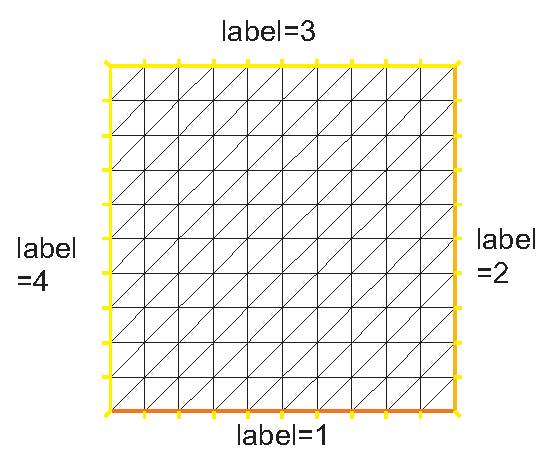
\includegraphics[height=6cm]{square}
\end{center}
  \caption{Boundary labels of the mesh by \texttt{square(10,10)}
  \label{fig:square}} \index{label}
\end{figure}
To construct a
$n\times m$ grid in the rectangle \index{rectangle} $[x_0,x_1]\times [y_0,y_1]$, proceeds as follows:
write
\bFF
  @real x0=1.2,x1=1.8;
  @real y0=0,y1=1;
  @int n=5,m=20;
  @mesh Th=@square(n,m,[x0+(x1-x0)*x,y0+(y1-y0)*y]);

\eFF

\begin{note}
Adding the  named  parameter \texttt{flags=icase} with icase:
\begin{description}
\item[0] will produce a mesh where all quads are split with diagonal $ x-y=cte$
\item[1] will produce Union Jack flag type of mesh.
\item[2] will produce a mesh where all quads are split with diagonal $ x+y=cte$ (v 3.8)
\item[3] same as case 0  except in two corners such that no triangle with 3 vertices on boundary (v 3.8)
\item[4] same as case 2  except in two corners such that no triangle with 3 vertices on boundary (v 3.8)
\end{description}\index{square!flags=}\index{square!label=}\index{square!region=}
\bFF
  @mesh Th=@square(n,m,[x0+(x1-x0)*x,y0+(y1-y0)*y],flags=icase);
\eFF
Adding the  named  parameter \texttt{label=labs} will change the 4 default
label numbers to \texttt{labs[i-1]}, for example \texttt{int[int] labs=[11,12,13,14]},

and adding the  named parameter \texttt{region=10} will change  the region number  to $10$,  for instance (v 3.8).

To see all these fags at work,  try the file \texttt{examples++/square-mesh.edp} :
\bFF
@for (@int i=0;i<5;++i)
  {
    @int[@int] labs=[11,12,13,14];
    @mesh Th=square(3,3,flags=i,label=labs,region=10);
    @plot(Th,wait=1,cmm=" square flags = "+i );
   }
\eFF

\end{note}


\subsubsection{\setS{Border}}\index{border}\index{label}

Boundaries are defined piecewise by parametrized curves.
The pieces can only intersect at their endpoints, but it is possible to 
join more than two endpoints. This can be used to structure the mesh
if an area thouches a border and create new regions by dividing larger ones:
\bFF
@int upper = 1;
@int others = 2;
@int inner = 3;

@border C01(t=0,1){x = 0;         y = -1+t;        label = upper;}
@border C02(t=0,1){x = 1.5-1.5*t; y = -1;          label = upper;}
@border C03(t=0,1){x = 1.5;       y = -t;          label = upper;}
@border C04(t=0,1){x = 1+0.5*t;   y = 0;           label = others;}
@border C05(t=0,1){x = 0.5+0.5*t; y = 0;           label = others;}
@border C06(t=0,1){x = 0.5*t;     y = 0;           label = others;}
@border C11(t=0,1){x = 0.5;       y = -0.5*t;      label = inner;}
@border C12(t=0,1){x = 0.5+0.5*t; y = -0.5;        label = inner;}
@border C13(t=0,1){x = 1;         y = -0.5+0.5*t;  label = inner;}

@int n = 10;
@plot(C01(-n)+C02(-n)+C03(-n)+C04(-n)+C05(-n)+C06(-n)+
      C11(n)+C12(n)+C13(n), wait=true);

@mesh Th = buildmesh(C01(-n)+C02(-n)+C03(-n)+C04(-n)+C05(-n)+C06(-n)+
      C11(n)+C12(n)+C13(n));

@plot(Th, wait=true); // figure \ref{multiendmesh}

@cout << "Part 1 has region number " << Th(0.75, -0.25).region << endl;
@cout << "Part 2 has redion number " << Th(0.25, -0.25).region << endl;
\eFF

%###
\twoplot[height=6cm]{multiendborder}{multiendmesh}{Multiple border ends intersect}{Generated mesh}

Triangulation keywords assume that the domain is defined as being on the \emph{left} (resp right) of its
oriented parameterized boundary
$$
\Gamma_j=\{(x,y)\left|\; x=\varphi_x(t),\, y=\varphi_y(t),\, a_j\le t\le b_j\right.\}
$$
To check the orientation plot
$t\mapsto (\varphi_x(t),\varphi_y(t)),\, t_0\le t\le t_1$.
If it is as in Fig. \ref{fig:border}, then
the domain lies on the shaded area, otherwise it lies on the opposite side


\begin{figure}[htbp]
\begin{center}
  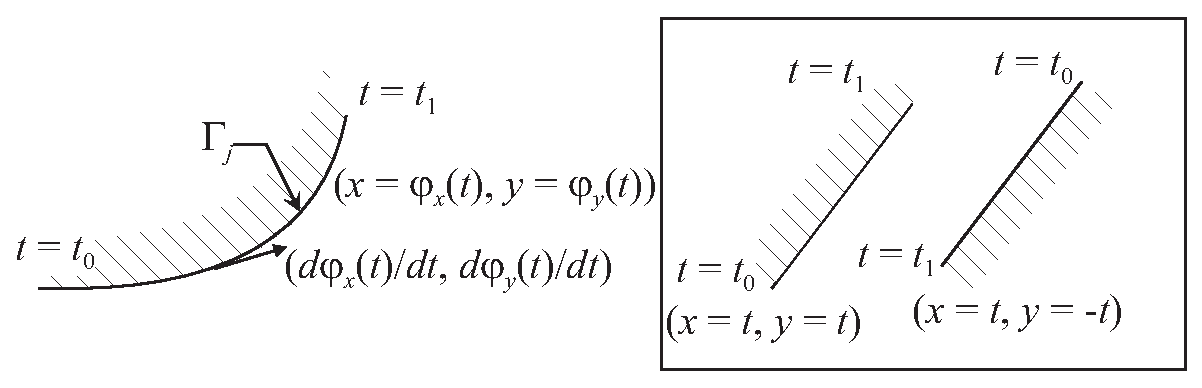
\includegraphics[height=4cm]{border}
\end{center}
  \caption{Orientation of the boundary defined by $(\phi_x(t),\phi_y(t))$
  \label{fig:border}} \index{border}
\end{figure}
The general expression to define a triangulation with \texttt{buildmesh} is
\begin{center}
\ttCC{@mesh  ~~Mesh_Name = @buildmesh}$\left(\Gamma_1(m_1)+\cdots+\Gamma_J(m_j) \mathrm{~OptionalParameter} \right)$;
\end{center}
where $m_j$ are positive or negative numbers to indicate how many vertices should be on $\Gamma_j,\,
\Gamma=\cup_{j=1}^J \Gamma_J$, and the optional parameter (separed with comma) can be
\begin{description}
\item[\texttt{nbvx=<int value>}] ,  to set the maximal number of  vertices in the mesh.\index{buildmesh!nbvx=}
\index{buildmesh!fixeborder=}
\item[\texttt{fixeborder=<bool value>}] , to say if the mesh generator can change the boundary mesh
or not (by default the boundary mesh can change; beware that with periodic boundary conditions 
(see. \ref{periodic BC}), it can be dangerous .\label{buildmesh fixeborder}\index{buildmesh!fixeborder}
\end{description}

The orientation of boundaries can be changed by changing the sign of $m_j$.
The following example shows how to change the orientation.
The example generates the unit disk
with a small circular hole, and assign ``1'' to the unit disk
(``2'' to the circle inside).
The boundary label must be non-zero, but it can also be omitted.

\bFF
1: @border a(t=0,2*pi){ x=cos(t); y=sin(t);label=1;}
2: @border b(t=0,2*pi){ x=0.3+0.3*cos(t); y=0.3*sin(t);label=2;}
3: @plot(a(50)+b(+30)) ; // to see a plot of the border mesh \index{plot!border}
4: @mesh Thwithouthole= @buildmesh(a(50)+b(+30));
5: @mesh Thwithhole   = @buildmesh(a(50)+b(-30));
6: @plot(Thwithouthole,wait=1,ps="Thwithouthole.eps"); //figure \ref{Thwithouthole}\index{plot!mesh}
7: @plot(Thwithhole,wait=1,ps="Thwithhole.eps"); // figure \ref{Thwithhole}
\eFF
\begin{note}
Notice that the orientation is changed by ``\texttt{b(-30)}'' in 5th line. In 7th line, \texttt{ps="fileName"} is used to generate a postscript file with identification shown on the figure.
\end{note}

\twoplot[height=6cm]{Thwithouthole}{Thwithhole}{mesh without hole}{mesh with hole}

\begin{note}
 Borders are evaluated only at the time \texttt{plot} or \texttt{buildmesh} is called  so
the global variable are defined  at this time andhere since $r$ is changed between the two border calls the following code will not work because the first border will be computed with r=0.3:
\bFF
   @real r=1;    @border a(t=0,2*pi){ x=r*cos(t); y=r*sin(t);label=1;}
   r=0.3    ;   @border b(t=0,2*pi){ x=r*cos(t); y=r*sin(t);label=1;}
   @mesh Thwithhole   = @buildmesh(a(50)+b(-30)); // bug (a trap) because
   // the two circle have the same radius = $0.3$
\eFF
\end{note}


\subsubsection{Data Structures and Read/Write Statements for a Mesh}

\index{readmesh}\index{savemesh}
Users who want to read a triangulation made elsewhere should see the structure
of the file generated below:
\bFF
@border C(t=0,2*pi) { x=cos(t); y=sin(t); }
@mesh Th = @buildmesh(C(10));
@savemesh("mesh_sample.msh");
\eFF
the mesh is shown on Fig. \ref{fig:meshSample}.
\\\\
The informations about \texttt{Th} are saved in the file ``mesh\_sample.msh''.
whose structure is shown on Table \ref{tab:meshSample}.
\\
There $n_v$ denotes
the number of vertices, $n_t$ number of triangles
and $n_s$ the number of edges on boundary.

For each vertex $q^i,\, i=1,\cdots,n_v$, denote   by $(q^i_x,q^i_y)$
the $x$-coordinate and $y$-coordinate.

Each triangle $T_k, k=1,\cdots,10$ has three vertices $q^{k_1},\, q^{k_2},\,q^{k_3}$
that are oriented counterclockwise.
The boundary consists of 10 lines $L_i,\, i=1,\cdots,10$ whose end points are
$q^{i_1},\, q^{i_2}$.

\begin{figure}[htbp]
\begin{minipage}{\textwidth}
\begin{minipage}{0.5\textwidth}
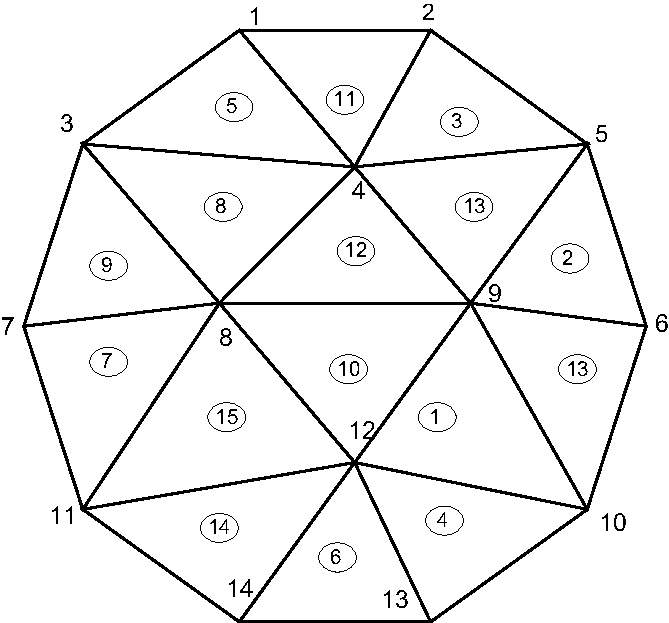
\includegraphics[width=\textwidth]{mesh_sample}%
\caption{mesh by \texttt{buildmesh(C(10))}
\label{fig:meshSample}}
\end{minipage}
\hspace{0.5mm}
\begin{minipage}{0.5\textwidth}
In the left figure, we have the following.\\\\
$n_v=14,\, n_t=16,\, n_s=10$\\\\
$q^1=(-0.309016994375,\, 0.951056516295)$\\
$\vdots\qquad \vdots\qquad \vdots$\\
$q^{14}=(-0.309016994375,\, -0.951056516295)$\\\\
The vertices of $T_1$ are $q^9,\, q^{12},\, q^{10}$.\\
$\vdots\qquad \vdots\qquad \vdots$\\
The vertices of $T_{16}$ are $q^9,\, q^{10},\, q^{6}$.\\\\
The edge of 1st side $L_1$ are $q^6,\, q^5$.\\
$\vdots\qquad \vdots\qquad \vdots$\\
The edge of 10th side $L_{10}$ are $q^{10},\, q^6$.\\
\end{minipage}
\end{minipage}
\end{figure}

\begin{table}[htbp]
\begin{tabular}{|l|l|}
\hline
Content of the file & Explanation\\
\hline
14 16 10& $n_v$\qquad  $n_t$\qquad $n_e$\\
-0.309016994375 0.951056516295 1& $q^1_x$\qquad $q^1_y$\qquad boundary label=1\\
0.309016994375 0.951056516295 1& $q^2_x$\qquad $q^2_y$\qquad boundary label=1\\
$\cdots$  $\cdots$ $\vdots$& \\
-0.309016994375 -0.951056516295 1& $q^{14}_x$\qquad $q^{14}_y$\qquad boundary label=1\\
\hline
9 12 10 0&$1_1$\quad $1_2$\quad $1_3$\quad region label=0 \\
5 9 6 0&$2_1$\quad $2_2$\quad $2_3$\quad region label=0  \\
$\cdots$& \\
9 10 6 0&$16_1$\quad $16_2$\quad $16_3$\quad region label=0 \\
\hline
6 5 1&$1_1\quad 1_2$\quad boundary label=1\\
5 2 1&$2_1\quad 2_2$\quad boundary label=1\\
$\cdots$& \\
10 6 1&$10_1\quad 10_2$\quad boundary label=1\\
\hline
\end{tabular}
  \caption{The structure of ``mesh\_sample.msh''
  \label{tab:meshSample}}
\end{table}

In \freefempp there are many mesh file formats available for communication with
other tools such as emc2, modulef.. (see \refSec{Mesh Files}),
The extension of a file implies its format. More details can be found on the file format .msh in the article by F. Hecht
"bamg : a bidimentional anisotropic mesh generator" (downloadable  from the
FreeFem web site. ) 
\\\\
 A
mesh file can be read into \freefempp except that the names of the
borders are lost and only their reference numbers are kept. So these borders have to be referenced by the number
which corresponds to their order of appearance in the program, unless
this number is overwritten by the keyword "label".  Here are some examples:

\bFF
@border floor(t=0,1){ x=t; y=0; label=1;}; // the unit square
@border right(t=0,1){ x=1; y=t; label=5;};
@border ceiling(t=1,0){ x=t; y=1; label=5;};
@border left(t=1,0){ x=0; y=t; label=5;};
@int n=10;
@mesh th= buildmesh(floor(n)+right(n)+ceiling(n)+left(n));
@savemesh(th,"toto.am_fmt");  // "formatted Marrocco" format \index{file!am\_fmt}
@savemesh(th,"toto.Th");      // "bamg"-type mesh   \index{file!bamg}
@savemesh(th,"toto.msh");     // freefem format \index{file!mesh}
@savemesh(th,"toto.nopo");     // modulef format \index{file!nopo} see \cite{modulef}
@mesh th2 = readmesh("toto.msh"); // read the mesh

\eFF

\begin{example}[Readmesh.edp]
\index{tutorial!readmesh.edp}
\index{read files}
\index{write files}
\bFF

@border floor(t=0,1){ x=t; y=0; label=1;}; // the unit square
@border right(t=0,1){ x=1; y=t; label=5;};
@border ceiling(t=1,0){ x=t; y=1; label=5;};
@border left(t=1,0){ x=0; y=t; label=5;};
@int n=10;
@mesh th= buildmesh(floor(n)+right(n)+ceiling(n)+left(n));
@savemesh(th,"toto.am_fmt");  // format "formated Marrocco" \index{file!am\_fmt}
@savemesh(th,"toto.Th");      // format database  db mesh "bamg"   \index{file!bamg}
@savemesh(th,"toto.msh");     // format freefem \index{file!mesh}
@savemesh(th,"toto.nopo");     // modulef format \index{file!nopo} see \cite{modulef}
@mesh th2 = readmesh("toto.msh");
@fespace femp1(th,@P1);
femp1 f = sin(x)*cos(y),g;
{ // save solution
@ofstream file("f.txt");
file << f[] << endl;
}  // close the file (end block)
{  // read
@ifstream file("f.txt");
file >> g[] ;
} // close reading file (end block)
@fespace Vh2(th2,P1);
Vh2 u,v;
@plot(g);
//  find $u$ such that \hfilll
// $ u + \Delta u = g $ in $\Omega $ , \hfilll
// $ u=0$ on $\Gamma_1$ and $\frac{\p u }{\p n} = g$ on $\Gamma_2$  \hfilll
@solve pb(u,v) =
    @int2d(th)( u*v - dx(u)*dx(v)-dy(u)*dy(v) )
  + @int2d(th)(-g*v)
  + @int1d(th,5)( g*v) //  $\frac{\p u }{\p n} = g$ on $\Gamma_2$
  + @on(1,u=0) ;
@plot (th2,u);
\eFF
\end{example}

\subsubsection{Mesh Connectivity}

The following example explains methods to obtain mesh information.

\index{mesh!connectivity}
\index{triangle![]}\index{triangle!label}\index{triangle!label}
\index{vertex!x}\index{vertex!y}\index{vertex!label}
\index{Element}
\index{whoinElement}
\index{adj}
\index{be}
\index{nbe}

\bFF
{ // get mesh information (version 1.37)
  @mesh Th=square(2,2);
  // get data of the mesh
  @int nbtriangles=Th.nt;
  cout << " nb of Triangles = " << nbtriangles << endl;
  @for (int i=0;i<nbtriangles;i++)
    @for (int j=0; j <3; j++)
      @cout << i << " " << j << " Th[i][j] = "
           << Th[i][j] << "  x = "<< Th[i][j].x  << " , y= "<< Th[i][j].y
           << ",  label=" << Th[i][j].label << endl;

//  \index{mesh!()}  Th(i)   return   the vextex i of Th\hfilll
//  \index{mesh![]} Th[k]   return   the triangle k of Th\hfilll

  @fespace femp1(Th,P1);
  femp1 Thx=x,Thy=y; //  hack of get vertex coordinates
  // get vertices information :
  @int nbvertices=Th.nv;
  cout << " nb of vertices = " << nbvertices << endl;
  @for (int i=0;i<nbvertices;i++)
        cout << "Th(" <<i  << ") : "   // << endl;
             << Th(i).x << " " << Th(i).y  << " " << Th(i).label //v 2.19
             << "       old method: " << Thx[][i] << " " << Thy[][i] << endl;

// method to find information of point (0.55,0.6)

  @int it00 = Th(0.55,0.6).nuTriangle;// \index{point!triange}then triangle number
  @int nr00 = Th(0.55,0.6).region; // \index{region}\index{point!region}

//  info of a triangle
  @real area00 = Th[it00].area; // new in version 2.19  \index{triangle!area}
  @real nrr00 = Th[it00].region; // new in version 2.19   \index{triangle!region}
  @real nll00 = Th[it00].label; // same as region in this case.  \index{triangle!label}


//Hack  to get a triangle containing point x,y\hfilll
//     or   region number (old method) \hfilll
// ------------------------------------------------------- \hfilll
  @fespace femp0(Th,P0);
  @femp0 nuT; // a P0 function  to get triangle numbering
    for (int i=0;i<Th.nt;i++)
     nuT[][i]=i;
  femp0 nuReg=region; // a P0 function to get the region number
  //  inquire
  @int it0=nuT(0.55,0.6);//number of triangle Th's containing (0.55,0,6);
  @int nr0=nuReg(0.55,0.6);//number of region of Th's containing (0.55,0,6);


 // dump  \hfilll
 // ------------------------------------------------------- \hfilll

  cout << "  point (0.55,0,6) :triangle number " << it00 << " " << it00
       << ", region = " << nr0 << " == " << nr00 << ",  area K " << area00 << endl;

  // new method to get boundary information and mesh adjacent

 @int k=0,l=1,e=1;
  Th.nbe ; // return the number of boundary element \hfilll
  Th.be(k);   // return the boundary element k $\in \{0,...,Th.nbe-1\}$ \hfilll
  Th.be(k)[l];   // return the vertices l $\in \{0,1\}$ of  boundary elmt k \hfilll
  Th.be(k).Element ;   // return the triangle containing the  boundary elmt k \hfilll
  Th.be(k).whoinElement ;   // return the edge number of triangle containing \hfilll
  //the  boundary elmt k
  Th[k].adj(e) ; // return adjacent triangle to k by edge e, and change \hfill
  // the value of e to the corresponding edge in the adjacent triangle
  Th[k] == Th[k].adj(e) // non adjacent triangle return the same
  Th[k] != Th[k].adj(e) // true adjacent triangle

  cout << " print mesh connectivity " << endl;
  @int nbelement = Th.nt;
  @for (@int k=0;k<nbelement;++k)
    @cout << k << " :  " << int(Th[k][0]) << " " << int(Th[k][1])
         << " " <<  int(Th[k][2])
         << " , label  " << Th[k].label << endl;
  //

  @for (@int k=0;k<nbelement;++k)
    @for (@int e=0,ee;e<3;++e)
      //  remark FH hack:  set ee to e, and ee is change by method adj,
      //  in () to make difference with  named parameters.
	    @cout << k <<  " " << e << " <=>  " << int(Th[k].adj((ee=e))) << " " << ee
	     << "  adj: " << ( Th[k].adj((ee=e)) != Th[k]) << endl;
      // note :     if k == int(Th[k].adj(ee=e)) not adjacent element


  @int nbboundaryelement = Th.nbe;

  @for (int k=0;k<nbboundaryelement;++k)
      cout << k << " : " <<  Th.be(k)[0] << " " << Th.be(k)[1] << " , label "
           << Th.be(k).label <<  " tria  " << int(Th.be(k).Element)
           << " " << Th.be(k).whoinElement <<  endl;

}
\eFF
the output is:
\bFF
 -- square mesh : nb vertices  =9 ,  nb triangles = 8 ,  nb boundary edges 8
    Nb of Vertices 9 ,  Nb of Triangles 8
    Nb of edge on user boundary  8 ,  Nb of edges on true boundary  8
 number of real boundary edges 8
 nb of Triangles = 8
0 0 Th[i][j] = 0  x = 0 , y= 0,  label=4
0 1 Th[i][j] = 1  x = 0.5 , y= 0,  label=1
0 2 Th[i][j] = 4  x = 0.5 , y= 0.5,  label=0
...
6 0 Th[i][j] = 4  x = 0.5 , y= 0.5,  label=0
6 1 Th[i][j] = 5  x = 1 , y= 0.5,  label=2
6 2 Th[i][j] = 8  x = 1 , y= 1,  label=3
7 0 Th[i][j] = 4  x = 0.5 , y= 0.5,  label=0
7 1 Th[i][j] = 8  x = 1 , y= 1,  label=3
7 2 Th[i][j] = 7  x = 0.5 , y= 1,  label=3
 Nb Of Nodes = 9
 Nb of DF = 9
 -- vector function's bound  0 1
 -- vector function's bound  0 1
 nb of vertices = 9
Th(0) : 0 0 4       old method: 0 0
Th(1) : 0.5 0 1       old method: 0.5 0
...
Th(7) : 0.5 1 3       old method: 0.5 1
Th(8) : 1 1 3       old method: 1 1
 Nb Of Nodes = 8
 Nb of DF = 8

 print mesh connectivity
0 :  0 1 4 , label  0
1 :  0 4 3 , label  0
...
6 :  4 5 8 , label  0
7 :  4 8 7 , label  0
0 0 <=>  3 1  adj: 1
0 1 <=>  1 2  adj: 1
0 2 <=>  0 2  adj: 0
...
6 2 <=>  3 0  adj: 1
7 0 <=>  7 0  adj: 0
7 1 <=>  4 0  adj: 1
7 2 <=>  6 1  adj: 1
0 : 0 1 , label 1 tria  0 2
1 : 1 2 , label 1 tria  2 2
...
6 : 0 3 , label 4 tria  1 1
7 : 3 6 , label 4 tria  5 1

\eFF


\subsubsection{The keyword "triangulate"}\index{triangulate}

\freefempp is able to build a triangulation from a set of points. This
triangulation is a Delaunay mesh of the convex hull of the set of points.
It can be useful to build a mesh form a table function.

The coordinates of the points and the value of the table function
are defined separately with rows of the form: \texttt{x y f(x,y)}
in a file such as:

\bFF
0.51387 0.175741 0.636237
0.308652 0.534534 0.746765
0.947628 0.171736 0.899823
0.702231 0.226431 0.800819
0.494773 0.12472 0.580623
0.0838988 0.389647 0.456045
...............
\eFF
%%% Thxy.eps not found
\twoplot[height=4cm]{Thxy}{xyf}{Delaunay mesh of the convex hull of point set in file xyf}
{Isovalue of table function}

The third column of each line is left untouched by the
\texttt{triangulate} command. But you can use this third value to
define a table function with rows of the form: \texttt{x y f(x,y)}.


The following example shows how to make a mesh from the file ``xyf''
with the format stated just above.
The command
\texttt{triangulate} command use only use 1st and 2nd rows.

\index{function!tables}

\bFF
@mesh Thxy=@triangulate("xyf"); // build the Delaunay mesh of the convex hull
// points are defined by the first 2 columns of file \texttt{xyf}
@plot(Thxy,ps="Thxyf.ps"); // (see figure  \ref{Thxy})

@fespace Vhxy(Thxy,P1); // create a P1 interpolation
Vhxy fxy; // the function

// reading the 3rd row to define the function
{ @ifstream file("xyf");
   @real xx,yy;
   @for(@int i=0;i<fxy.n;i++)
   file >> xx >>yy >> fxy[][i];  // to read third row only.
   // xx and yy are just skipped
}
@plot(fxy,ps="xyf.eps"); // plot the function (see figure  \ref{xyf})
\eFF

One  new way to build a mesh is to have two arrays one  the $x$ values and the other for the $y$ values (version 2.23-2):
\bFF
Vhxy xx=x,yy=y;// to set two arrays for the x's and y's
@mesh Th=@triangulate(xx[],yy[]);
\eFF

\subsection{Boundary FEM Spaces Built as Empty Meshes}\index{emptymesh}
To define a Finite Element space on a boundary,
we came up with the idea of a mesh with no internal points (call empty mesh).
It can be useful to handle Lagrange multipliers in mixed and mortar methods.

So the function \texttt{emptymesh} remove all the internal points of a mesh except
points  on  internal boundaries.

\bFF
{  //  new stuff 2004 emptymesh (version 1.40)
 // -- useful to build Multiplicator space
 //  build a mesh without internal point
 // with the same boundary
 //  -----
  assert(version>=1.40);
  @border a(t=0,2*pi){ x=cos(t); y=sin(t);label=1;}
  @mesh Th=buildmesh(a(20));
   Th=@emptymesh(Th);
  @plot(Th,wait=1,ps="emptymesh-1.eps");//see figure \ref{fig emptymesh-1}
}
\eFF

It is also possible to build an empty mesh of a pseudo subregion
with \texttt{emptymesh(Th,ssd)} using the set of edges of the mesh \texttt{Th};
a edge $e$ is in  this set  if with the two adjacent triangles $e =t1\cap t2$
and  $ ssd[T1] \neq ssd[T2]$ where \texttt{ssd}  refers to the pseudo region
numbering of triangles, when they are stored in an \texttt{int[int]} array of size the number of triangles.
\bFF
{  //  new stuff 2004 emptymesh (version 1.40) \hfilll
 // -- useful to build Multiplicator space \hfilll
 //  build a mesh without internal point \hfilll
 // of peusdo sub domain  \hfilll
 //  ----- \hfilll
  @assert(version>=1.40);
  @mesh Th=@square(10,10);
  @int[@int] ssd(Th.nt);
  @for(@int i=0;i<ssd.n;i++) // build the  pseudo region numbering
   {  @int iq=i/2;   // because 2 triangle per quad
      @int ix=iq%10; //
      @int iy=iq/10; //
    ssd[i]= 1 + (ix>=5) +  (iy>=5)*2;
   }
  Th=@emptymesh(Th,ssd); // build emtpy  with
  //  all edge $e = T1 \cap T2$ and $ ssd[T1] \neq ssd[T2]$
  @plot(Th,wait=1,ps="emptymesh-2.eps");//see figure \ref{fig emptymesh-2}
  @savemesh(Th,"emptymesh-2.msh");
}
\eFF

\twoplot[height=6cm]{emptymesh-1}{emptymesh-2}{ The empty mesh with boundary
\label{fig emptymesh-1}}{An empty mesh
defined from a pseudo region numbering of triangle\label{fig emptymesh-2}}

\subsection{Remeshing}
\subsubsection{\setS{Movemesh}}\index{movemesh}\index{checkmovemesh}

Meshes can be translated, rotated and deformed by {\tt movemesh}; this is useful for
 elasticity to watch the deformation due to the displacement
$\vec\Phi(x,y)=(\Phi_1(x,y),\Phi_2(x,y))$ of shape. It is also useful to
handle free boundary  problems or optimal shape problems.

If $\Omega$ is triangulated as $T_h(\Omega)$,
and $\Phi$ is a displacement vector then $\Phi(T_h)$ is obtained by
\bFF
@mesh  Th=@movemesh(Th,[$\Phi$1,$\Phi$2]);
\eFF
Sometimes the transformed mesh is invalid because some triangle
have flip over (now has negative area).To spot such problems one may check the
minimum triangle area in the transformed mesh with
\texttt{checkmovemesh} before any real transformation.

\begin{example} $\Phi_1(x,y)=x+k*\sin(y*\pi)/10)$,
$\Phi_2(x,y)=y+k*\cos(y\pi)/10)$ for a big number $k>1$.
\bFF
verbosity=4;
@border a(t=0,1){x=t;y=0;label=1;};
@border b(t=0,0.5){x=1;y=t;label=1;};
@border c(t=0,0.5){x=1-t;y=0.5;label=1;};
@border d(t=0.5,1){x=0.5;y=t;label=1;};
@border e(t=0.5,1){x=1-t;y=1;label=1;};
@border f(t=0,1){x=0;y=1-t;label=1;};
@func uu= sin(y*pi)/10;
@func vv= cos(x*pi)/10;

@mesh Th = buildmesh ( a(6) + b(4) + c(4) +d(4) + e(4) + f(6));
@plot(Th,wait=1,fill=1,ps="Lshape.eps");// see figure \ref{lshape}
@real coef=1;
@real minT0= @checkmovemesh(Th,[x,y]); // the min triangle area
@while(1) // find a correct move mesh
{
  @real minT=@checkmovemesh(Th,[x+coef*uu,y+coef*vv]);//the min triangle area
  if (minT > minT0/5) break ; // if big enough
  coef/=1.5;
}

Th=@movemesh(Th,[x+coef*uu,y+coef*vv]);
@plot(Th,wait=1,fill=1,ps="movemesh.eps");// see figure \ref{movemesh}
\eFF

\twoplot[height=6cm]{lshape}{movemesh}{L-shape}{  moved L-shape }
\end{example}
\begin{note}
Consider a function $u$ defined on a mesh \texttt{Th}. A statement like
\texttt{Th=movemesh(Th...)} does not change $u$ and so the old mesh
still exists. It will be destroyed when no function use it. A
statement like $u=u$ redefines $u$ on the new mesh \texttt{Th} with
interpolation and therefore destroys the old \texttt{Th} if $u$ was the only
function using it.
\end{note}

\begin{example}[movemesh.edp]
\index{tutorial!movemesh.edp}
Now, we given an example of moving mesh with a lagrangian\index{lagrangian}
function $u$ defined on the moving mesh.

\bFF
// simple movemesh example
@mesh Th=square(10,10);
@fespace Vh(Th,P1);
@real t=0;
// ---
//  the problem is how to build data without interpolation
//  so the data u is moving with the mesh as you can see in the plot
// ---
Vh u=y;
@for (int i=0;i<4;i++)
{
 t=i*0.1;
 Vh f= x*t;
 @real minarea=checkmovemesh(Th,[x,y+f]);
 if (minarea >0 ) // movemesh will be ok
   Th=movemesh(Th,[x,y+f]);

 cout << " Min area  " << minarea << endl;

 real[int] tmp(u[].n);
 tmp=u[];  // save the value
 u=0;        // to change the FEspace and mesh associated with u
 u[]=tmp;  // set the value of u without any mesh update
 @plot(Th,u,wait=1);
};
// In this program, since u is only defined on the last mesh, all the \hfilll
// previous meshes are deleted from memory.  \hfilll
//   --------  \hfilll
\eFF
\end{example}

\subsection{\setS{Regular Triangulation}: {\tt hTriangle}}
For a set $S$, we define the diameter of $S$ by
\[
\textrm{diam}(S)=\sup\{|\vec{x}-\vec{y}|; \; \vec{x},\, \vec{y}\in S\}
\]
The sequence $\{\mathcal{T}_h\}_{h\downarrow 0}$ of $\Omega$ is called
\emph{regular}\index{mesh!regular} if they satisfy the following:
\begin{enumerate}
  \item
\[
\lim_{h\downarrow 0}\max\{\textrm{diam}(T_k)|\; T_k\in \mathcal{T}_h\}=0
\]
  \item
There is a number $\sigma>0$ independent of $h$ such that
\[
\frac{\rho(T_k)}{\textrm{diam}(T_k)}\ge \sigma
\qquad \textrm{for all }T_k\in \mathcal{T}_h
\]
where $\rho(T_k)$ are the diameter of the inscribed circle of $T_k$.
\end{enumerate}
We put $h(\mathcal{T}_h)=\max\{\textrm{diam}(T_k)|\; T_k\in \mathcal{T}_h\}$,
which is obtained by
\bFF
@mesh Th = ......;
@fespace Ph(Th,P0);
Ph h = @hTriangle;
@cout << "size of mesh = " << h[].max << @endl;
\eFF

\subsection{Adaptmesh}\index{adaptmesh}\index{adaptation}\index{mesh!adaptation}
\label{sec:Adaptmesh}
The function
\[
f(x,y) = 10.0x^3+y^3+\tan^{-1}[\varepsilon/(\sin(5.0y)-2.0x)]
\qquad \varepsilon =  0.0001
\]
sharply varies in value and the initial mesh given by one of the commands of Section \ref{sec:InitialMesh}
cannot reflect its sharp variations.
\begin{example}~
\bFF
@real eps =  0.0001;
@real h=1;
@real hmin=0.05;
@func f = 10.0*x^3+y^3+h*atan2(eps,sin(5.0*y)-2.0*x);

@mesh Th=square(5,5,[-1+2*x,-1+2*y]);
@fespace Vh(Th,P1);
Vh fh=f;
@plot(fh);
for (@int i=0;i<2;i++)
 {
   Th=@adaptmesh(Th,fh);
   fh=f;  // old mesh is deleted
   @plot(Th,fh,wait=1);
 }
\eFF
\end{example}
\plot[height=10cm]{adaptmesh}{3D graphs for the initial mesh and 1st and 2nd mesh adaptation}

\freefempp uses a variable metric/Delaunay automatic meshing
algorithm.
The command
\bFF
@mesh ATh = @adaptmesh(Th, f);
\eFF
create the new mesh \texttt{ATh} adapted to the Hessian
$$
D^2f=(\p^2 f/\p x^2,\, \p^2 f/\p x\p y,
\p^2 f/\p y^2)
$$
of a function (formula or FE-function).
Mesh adaptation is a very powerful tool when the solution of a problem
varies locally and sharply.

Here we solve the problem (\ref{eqn:Poisson})-(\ref{eqn:Dirichlet}),
when $f=1$ and $\Omega$ is a L-shape domain.

\twoplot[height=5cm]{L-shape2}{lshapeSol}{ L-shape domain and its boundary name}{Final solution after 4-times adaptation}


\begin{example}[Adapt.edp]
\index{tutorial!adapt.edp}
The solution has the
\index{singularity}singularity $r^{3/2},\, r=|x-\gamma|$
at the point $\gamma$ of the intersection of two lines
$bc$ and $bd$ (see Fig. \ref{L-shape2}).
\bFF
@border ba(t=0,1.0){x=t;   y=0;  label=1;};
@border bb(t=0,0.5){x=1;   y=t;  label=1;};
@border bc(t=0,0.5){x=1-t; y=0.5;label=1;};
@border bd(t=0.5,1){x=0.5; y=t;  label=1;};
@border be(t=0.5,1){x=1-t; y=1;  label=1;};
@border bf(t=0.0,1){x=0;   y=1-t;label=1;};
@mesh Th = @buildmesh ( ba(6)+bb(4)+bc(4)+bd(4)+be(4)+bf(6) );
@fespace Vh(Th,@P1);  // set FE space
Vh u,v;             // set unknown and test function
func f = 1;
@real error=0.1;        // level of error
@problem Poisson(u,v,solver=CG,eps=1.0e-6) =
    @int2d(Th)(  dx(u)*dx(v) + dy(u)*dy(v))
  - @int2d(Th) ( f*v )
  + @on(1,u=0)  ;
@for (@int i=0;i< 4;i++)
{
  Poisson;
  Th=@adaptmesh(Th,u,err=error);
  error = error/2;
} ;
@plot(u);
\eFF
\end{example}
To speed up the adaptation
the default parameter \texttt{err} of
\texttt{adaptmesh}\index{concatenation} is changed by hand; it
specifies the required precision, so as to make the new mesh finer or coarser.

The problem is coercive and symmetric,
so the linear system can be solved with the conjugate gradient
method \index{solver=!CG} (parameter \texttt{solver=CG}
with the stopping criteria on the residual, here
\texttt{eps=1.0e-6}).
By \texttt{adaptmesh}, the slope of the final solution is correctly computed near
the point of intersection of $bc$ and $bd$ as in Fig. \ref{lshapeSol}.

This method is described in detail in \cite{bamg}. It has a number of
default parameters which can be modified~:

\index{adaptmesh}

Si \texttt{f1,f2} sont des functions  et \texttt{thold, Thnew} des maillages.
\bFF
    Thnew = @adaptmesh(Thold, f1  ...  );
    Thnew = @adaptmesh(Thold, f1,f2  ...  ]);
    Thnew = @adaptmesh(Thold, [f1,f2]  ...  );
\eFF
The additional paramters of  adaptmesh not written here, hence the  "..."
\begin{description}

    \item[\texttt{hmin=}] Minimum edge size.  \index{adaptmesh!hmin=}
    ({\tt val} is a real. Its default is related to
    the size of the domain to be meshed and the precision of the mesh
    generator).

    \item[\texttt{hmax=}] Maximum edge size.  ({\tt val} is a real.
    It defaults to the diameter of the domain to be
    meshed) \index{adaptmesh!hmax=}

    \item[\texttt{err=}] $P_1$ interpolation error level (0.01 is the
    default).  \index{adaptmesh!err=}

    \item[\texttt{errg=}] Relative geometrical error. By default this
    error is 0.01, and in any case it must be lower than $1/\sqrt{2}$.
    Meshes created with this option may have some edges smaller than
    the {\tt -hmin } due to geometrical constraints.
    \index{adaptmesh!errg=}

    \item[\texttt{nbvx=}] Maximum number of vertices generated by the
    mesh generator (9000 is the default).
    \index{adaptmesh!nbvx=}

    \item[\texttt{nbsmooth=}] number of iterations of the smoothing
    procedure (5 is the default).  \index{adaptmesh!nbsmooth=}

    \item[\texttt{nbjacoby=}] number of iterations in a smoothing
    procedure during the metric construction, 0 means no smoothing (6
    is the default).  \index{adaptmesh!nbjacoby=}

    \item[\texttt{ratio=}] ratio for a prescribed smoothing on the
    metric.  If the value is 0 or less than 1.1 no smoothing is done
    on the metric (1.8 is the default).

    If \texttt{ratio} $> 1.1$, the speed of mesh size variations is
    bounded by $log(\mathtt{ratio})$.  Note: As {\tt ratio} gets
    closer to {\tt 1}, the number of generated vertices increases.
    This may be useful to control the thickness of refined regions
    near shocks or boundary layers .  \index{adaptmesh!ratio=}

   \item[\texttt{omega=}] relaxation parameter for the smoothing
   procedure (1.0 is the default).  \index{adaptmesh!omega=}

    \item[\texttt{iso=}] If true, forces the metric to be isotropic
    (false is the default).  \index{adaptmesh!iso=}

    \item[\texttt{abserror=}] If false, the metric is evaluated using
    the criterium of equi-repartion of relative error (false is the
    default).  In this case the metric is defined by

\begin{equation}
  \mathcal{M} = \left({1\over\mathtt{err}\,\, \mathtt{coef}^2} \quad {
  |\mathcal{H}| \over max(\mathtt{CutOff},|\eta|)}\right)^p
  \label{eq err rel}
\end{equation}
    \index{adaptmesh!abserror=}

    otherwise, the metric is evaluated using the criterium of
    equi-distribution of errors.  In this case the metric is defined
    by

\begin{equation}
  \mathcal{M} = \left({1\over \mathtt{err}\,\,\mathtt{coef}^2} \quad
  {|{\mathcal{H}|} \over
  {\sup(\eta)-\inf(\eta)}}\right)^p.\label{eq err abs}
\end{equation}

    \item[\texttt{cutoff=}] lower limit for the relative error
    evaluation (1.0e-6 is the default).
    \index{adaptmesh!cutoff=}

    \item[\texttt{verbosity=}] informational messages level (can be
    chosen between 0 and $\infty$). Also changes the value of the
    global variable verbosity (obsolete).  \index{adaptmesh!verbosity=}

    \item[\texttt{inquire=}] To inquire graphically about the mesh (false is the
    default).  \index{adaptmesh!inquire=}

    \item[\texttt{splitpbedge=}] If true, splits all internal edges in
    half with two boundary vertices (true is the default).
    \index{adaptmesh!splitpbedge=}

    \item[\texttt{maxsubdiv=}] Changes the metric such that the
    maximum subdivision of a background edge is bound by {\tt val}
    (always limited by 10, and 10 is also the default).
    \index{adaptmesh!maxsubdiv=}

    \item[\texttt{rescaling=}] if true, the function with respect to
    which the mesh is adapted is rescaled to be between 0 and 1 (true
    is the default).  \index{adaptmesh!rescaling=}

    \item[\texttt{keepbackvertices=}] if true, tries to keep as many
    vertices from the original mesh as possible (true is the default).
    \index{adaptmesh!keepbackvertices=}

    \item[\texttt{isMetric=}] if true, the metric is defined
    explicitly (false is the default).  If the 3 functions $m_{11},
    m_{12}, m_{22}$ are given, they directly define a symmetric matrix
    field whose Hessian is computed to define a metric. If only one
    function is given, then it represents the isotropic mesh size at
    every point.  \index{adaptmesh!IsMetric=}

    For example, if the partial derivatives
    \texttt{fxx} ($=\p^2 f/\p x^2$),
    \texttt{fxy} ($=\p^2 f/\p x\p y$),
    \texttt{fyy} ($=\p^2 f/\p y^2$) are given, we can set
    $$
    \ttCC{Th=@adaptmesh(Th,fxx,fxy,fyy,IsMetric=1,nbvx=10000,hmin=hmin);}
    $$

    \item[\texttt{power=}] exponent power of the Hessian used to
    compute the metric (1 is the default).  \index{adaptmesh!powerin=}

\index{adaptmesh!thetamax=}
    \item[\texttt{thetamax=}] minimum corner  angle of in degrees (default
    is $10^\circ$) where the corner is $ABC$ and the angle is the angle of the two vectors  ${AB}, {BC}$, 
    ($0$ imply no corner, $90$ imply perp. corner , ...). 

    \item[\texttt{splitin2=}] boolean value. If true, splits all
    triangles of the final mesh into 4
    sub-triangles. \index{adaptmesh!splitin2=}

    \item[\texttt{metric=}] \index{adaptmesh!metric=} an array of 3
    real arrays to set or get metric data information. The size of
    these three arrays must be the number of vertices. So if
    \texttt{m11,m12,m22} are three P1 finite elements related to the
    mesh to adapt, you can write: \texttt{metric=[m11[],m12[],m22[]]}
    (see file convect-apt.edp for a full example)

    \itemtt[nomeshgeneration=] \index{adaptmesh!nomeshgeneration=} If
    true, no adapted mesh is generated (useful to compute only a
    metric).

    \itemtt[periodic=] \index{adaptmesh!periodic=} %%% modif FH
    Writing \texttt{periodic=[[4,y],[2,y],[1,x],[3,x]];}
    builds an adapted periodic mesh. The sample
    build a biperiodic mesh of a square.
    (see periodic finite element   spaces \ref{periodic BC}, and see \texttt{sphere.edp} for a  full example)
\end{description}

%%%alh proofreading ok up to here


 We can use the command \ttCC{adaptmesh} to build uniform mesh with a
 contant mesh size. \index{mesh!uniform}\index{adaptmesh!uniform}

 So to build a mesh with a constant mesh size equal to $\frac{1}{30}$ try:

\begin{example}{uniformmesh.edp} 
\bFF
@mesh Th=square(2,2); // to have initial mesh
plot(Th,wait=1,ps="square-0.eps");
Th= @adaptmesh(Th,1./3As writing
0.,IsMetric=1,nbvx=10000);// \index{mesh!uniform}
plot(Th,wait=1,ps="square-1.eps");
Th= @adaptmesh(Th,1./30.,IsMetric=1,nbvx=10000);//  more the one time du to
Th= @adaptmesh(Th,1./30.,IsMetric=1,nbvx=10000);//  adaptation  bound \texttt{maxsubdiv=}
plot(Th,wait=1,ps="square-2.eps");
\eFF
\threeplot[width=5cm]%
{square-0}{Initial mesh}%
{square-1}{first iteration}%
{square-2}{last iteration}%
\end{example}

\subsection{Trunc}\index{trunc}

Two operators have been introduce to remove triangles from a mesh or to divide them.
Operator {\tt trunc } has two parameters
% FFCS(8/10/9)need to move index for htindex not to interfere
% with \begin{description}
\index{split=} \index{label=}\index{trunc!split=} \index{trunc!label=}
\begin{description}
  \itemtt[label=] sets the label number of new boundary item (one by default)
  \itemtt[split=] sets the level $n$ of triangle splitting. each triangle is splitted in  $n\times n$ ( one by default).
\end{description}

To create the mesh \texttt{Th3}
where alls  triangles of a mesh \texttt{Th}  are splitted in $3{\times}3$ , just write:
\bFF
  mesh Th3 = trunc(Th,1,split=3);
\eFF

The  \texttt{truncmesh.edp} example construct
all "trunc" mesh  to the support of the basic function  of the space \texttt{Vh} (cf. \texttt{abs(u)>0}),
split all the  triangles in $5{\times} 5$, and put a label number to $2$ on new boundary.
\bFF
@mesh Th=square(3,3);
@fespace Vh(Th,P1);
Vh u;
@int i,n=u.n;
u=0;
@for (i=0;i<n;i++)  // all degree of freedom
 {
  u[][i]=1;        //  the basic function i
  @plot(u,wait=1);
  @mesh Sh1=trunc(Th,abs(u)>1.e-10,split=5,label=2);
  plot(Th,Sh1,wait=1,ps="trunc"+i+".eps");// plot the mesh of
  // the function's support
  u[][i]=0;      // reset
 }
\eFF
\twoplot[height=6cm]{trunc0}{trunc6}{ mesh of support the function P1  number 0, splitted in $5{\times}5$ }{
mesh of support the function P1  number 6, splitted in $5{\times}5$ }
\index{splitmesh}
\subsection{Splitmesh}
Another way to split mesh triangles is to use {\tt splitmesh}, for example:
\bFF
{  //  new stuff 2004 splitmesh (version 1.37)
  assert(version>=1.37);
  @border a(t=0,2*pi){ x=cos(t); y=sin(t);label=1;}
  @mesh Th=@buildmesh(a(20));
  @plot(Th,wait=1,ps="nosplitmesh.eps"); // see figure \ref{fig nosplitmesh}
  @Th=@splitmesh(Th,1+5*(square(x-0.5)+y*y));
  @plot(Th,wait=1,ps="splitmesh.eps"); // see figure \ref{fig splitmesh}
}
\eFF

\twoplot[height=6cm]{nosplitmesh}{splitmesh}{\label{fig nosplitmesh}initial mesh}{\label{fig splitmesh}all left mesh triangle is split  conformaly in \texttt{int(1+5*(square(x-0.5)+y*y)\^2} triangles.}


\subsection{\setS{Meshing Examples}}

\begin{example}[Two rectangles touching by a side]~
\index{mesh!beam}
\bFF
@border a(t=0,1){x=t;y=0;};
@border b(t=0,1){x=1;y=t;};
@border c(t=1,0){x=t ;y=1;};
@border d(t=1,0){x = 0; y=t;};
@border c1(t=0,1){x=t ;y=1;};
@border e(t=0,0.2){x=1;y=1+t;};
@border f(t=1,0){x=t ;y=1.2;};
@border g(t=0.2,0){x=0;y=1+t;};
@int n=1;
@mesh th = @buildmesh(a(10*n)+b(10*n)+c(10*n)+d(10*n));
@mesh TH = @buildmesh ( c1(10*n) + e(5*n) + f(10*n) + g(5*n) );
@plot(th,TH,ps="TouchSide.esp"); // Fig. \ref{TouchSide}
\eFF
\end{example}

\begin{example}[NACA0012 Airfoil]~
\index{mesh!NACA0012}
\bFF
@border upper(t=0,1) { x = t;
     y = 0.17735*sqrt(t)-0.075597*t
  - 0.212836*(t^2)+0.17363*(t^3)-0.06254*(t^4); }
@border lower(t=1,0) { x = t;
     y= -(0.17735*sqrt(t)-0.075597*t
  -0.212836*(t^2)+0.17363*(t^3)-0.06254*(t^4)); }
@border c(t=0,2*pi) { x=0.8*cos(t)+0.5;  y=0.8*sin(t); }
@mesh Th = @buildmesh(c(30)+upper(35)+lower(35));
@plot(Th,@ps="NACA0012.eps",@bw=1);  // Fig. \ref{NACA0012}
\eFF
\end{example}

\twoplot[height=5cm]{TouchSide}{NACA0012}{Two rectangles touching by a side}
{NACA0012 Airfoil}

\begin{example}[Cardioid]~
\index{mesh!Cardioid}
\bFF
@real b = 1, a = b;
@border C(t=0,2*pi) { x=(a+b)*cos(t)-b*cos((a+b)*t/b);
                        y=(a+b)*sin(t)-b*sin((a+b)*t/b); }
@mesh Th = @buildmesh(C(50));
@plot(Th,@ps="Cardioid.eps",bw=1); // Fig. \ref{Cardioid}
\eFF
\end{example}
\begin{example}[Cassini Egg]~
\index{mesh!Cassini Egg}
\bFF
@border C(t=0,2*pi) { x=(2*cos(2*t)+3)*cos(t);
                      y=(2*cos(2*t)+3)*sin(t); }
@mesh Th = @buildmesh(C(50));
@plot(Th,@ps="Cassini.eps",bw=1); // Fig. \ref{Cassini}
\eFF
\end{example}
\twoplot[height=5cm]{Cardioid}{Cassini}{Domain with Cardioid curve boundary}
{Domain with Cassini Egg curve boundary}

\begin{example}[By cubic Bezier curve]~
\index{mesh!Bezier curve}
\bFF
// A cubic Bezier curve connecting two points with two control points
@func @real @bzi(@real p0,@real p1,@real q1,@real q2,@real t)
{
  @return p0*(1-t)^3+q1*3*(1-t)^2*t+q2*3*(1-t)*t^2+p1*t^3;
}

real[int] p00=[0,1], p01=[0,-1], q00=[-2,0.1], q01=[-2,-0.5];
real[int] p11=[1,-0.9], q10=[0.1,-0.95], q11=[0.5,-1];
real[int] p21=[2,0.7], q20=[3,-0.4], q21=[4,0.5];
real[int] q30=[0.5,1.1], q31=[1.5,1.2];
@border G1(t=0,1) { x=bzi(p00[0],p01[0],q00[0],q01[0],t);
                   y=bzi(p00[1],p01[1],q00[1],q01[1],t); }
@border G2(t=0,1) { x=bzi(p01[0],p11[0],q10[0],q11[0],t);
                   y=bzi(p01[1],p11[1],q10[1],q11[1],t); }
@border G3(t=0,1) { x=bzi(p11[0],p21[0],q20[0],q21[0],t);
                   y=bzi(p11[1],p21[1],q20[1],q21[1],t); }
@border G4(t=0,1) { x=bzi(p21[0],p00[0],q30[0],q31[0],t);
                   y=bzi(p21[1],p00[1],q30[1],q31[1],t); }
@int m=5;
@mesh Th = @buildmesh(G1(2*m)+G2(m)+G3(3*m)+G4(m));
@plot(Th,ps="Bezier.eps",bw=1);  // Fig \ref{Bezier}
\eFF
\end{example}

\begin{example}[Section of Engine]~
\index{mesh!Section of Engine}
\bFF
real a= 6., b= 1., c=0.5;
border L1(t=0,1) { x= -a; y= 1+b - 2*(1+b)*t; }
border L2(t=0,1) { x= -a+2*a*t; y= -1-b*(x/a)*(x/a)*(3-2*abs(x)/a );}
border L3(t=0,1) { x= a; y=-1-b + (1+ b )*t; }
border L4(t=0,1) { x= a - a*t;   y=0; }
border L5(t=0,pi) { x= -c*sin(t)/2; y=c/2-c*cos(t)/2; }
border L6(t=0,1) { x= a*t;  y=c; }
border L7(t=0,1) { x= a;  y=c + (1+ b-c )*t; }
border L8(t=0,1) { x= a-2*a*t; y= 1+b*(x/a)*(x/a)*(3-2*abs(x)/a); }
mesh Th = buildmesh(L1(8)+L2(26)+L3(8)+L4(20)+L5(8)+L6(30)+L7(8)+L8(30));
plot(Th,ps="Engine.eps",bw=1); // Fig. \ref{Engine}
\eFF
\end{example}

\begin{figure}[hbt]
\begin{multicols}{2}
\begin{center}
\includegraphics*[height=5cm]{Bezier}
\caption{\label{Bezier} Boundary drawed by Bezier curves}
\end{center}
\begin{center}
\vspace{3cm}~~\\
\includegraphics*[height=2.8cm]{Engine}
\caption{\label{Engine} Section of Engine}
\end{center}
\end{multicols}
\end{figure}

\begin{example}[Domain with U-shape channel]~
\index{mesh!U-shape channel}
\bFF
@real d = 0.1; // width of U-shape
@border L1(t=0,1-d) { x=-1; y=-d-t; }
@border L2(t=0,1-d) { x=-1; y=1-t; }
@border B(t=0,2) { x=-1+t; y=-1; }
@border C1(t=0,1) { x=t-1; y=d; }
@border C2(t=0,2*d) { x=0; y=d-t; }
@border C3(t=0,1) { x=-t; y=-d; }
@border R(t=0,2) { x=1; y=-1+t; }
@border T(t=0,2) { x=1-t; y=1; }
@int n = 5;
@mesh Th = buildmesh (L1(n/2)+L2(n/2)+B(n)+C1(n)+C2(3)+C3(n)+R(n)+T(n));
@plot(Th,ps="U-shape.eps",bw=1); // Fig \ref{U-shape}
\eFF
\end{example}
\begin{example}[Domain with V-shape cut]~
\index{mesh!V-shape cut}
\bFF
@real dAg = 0.01; // angle of V-shape
@border C(t=dAg,2*pi-dAg) { x=cos(t); y=sin(t); };
@real[int] pa(2), pb(2), pc(2);
pa[0] = cos(dAg); pa[1] = sin(dAg);
pb[0] = cos(2*pi-dAg); pb[1] = sin(2*pi-dAg);
pc[0] = 0; pc[1] = 0;
@border seg1(t=0,1) { x=(1-t)*pb[0]+t*pc[0]; y=(1-t)*pb[1]+t*pc[1]; };
@border seg2(t=0,1) { x=(1-t)*pc[0]+t*pa[0]; y=(1-t)*pc[1]+t*pa[1]; };
@mesh Th = @buildmesh(seg1(20)+C(40)+seg2(20));
@plot(Th,@ps="V-shape.eps",@bw=1);  // Fig. \ref{V-shape}
\eFF
\end{example}
\twoplot[height=5cm]{U-shape}{V-shape}{Domain with U-shape channel changed by \texttt{d}}
{Domain with V-shape cut changed by \texttt{dAg}}

\begin{example}[Smiling face]~
\index{mesh!Smiling face}
\bFF
@real d=0.1;
@int m=5;
@real a=1.5, b=2, c=0.7, e=0.01;
@border F(t=0,2*pi) { x=a*cos(t); y=b*sin(t); }
@border E1(t=0,2*pi) { x=0.2*cos(t)-0.5; y=0.2*sin(t)+0.5; }
@border E2(t=0,2*pi) { x=0.2*cos(t)+0.5; y=0.2*sin(t)+0.5; }
@func @real @st(real t) {
   @return sin(pi*t)-pi/2;
}
@border C1(t=-0.5,0.5) { x=(1-d)*c*cos(st(t)); y=(1-d)*c*sin(st(t)); }
@border C2(t=0,1){x=((1-d)+d*t)*c*cos(st(0.5));y=((1-d)+d*t)*c*sin(st(0.5));}
@border C3(t=0.5,-0.5) { x=c*cos(st(t)); y=c*sin(st(t)); }
@border C4(t=0,1) { x=(1-d*t)*c*cos(st(-0.5)); y=(1-d*t)*c*sin(st(-0.5));}

@border C0(t=0,2*pi) { x=0.1*cos(t); y=0.1*sin(t); }
@mesh Th=@buildmesh(F(10*m)+C1(2*m)+C2(3)+C3(2*m)+C4(3)
                  +C0(m)+E1(-2*m)+E2(-2*m));
@plot(Th,@ps="SmileFace.eps",@bw=1);  // see Fig. \ref{SmileFace}
}\eFF
\end{example}

\begin{example}[3point bending]~
\index{mesh!3point bending}
\bFF
// Square for Three-Point Bend Specimens fixed on \ttCC{Fix1, Fix2}
// It will be loaded on \ttCC{Load}.
@real a=1, b=5, c=0.1;
@int n=5, m=b*n;
@border Left(t=0,2*a) { x=-b; y=a-t; }
@border Bot1(t=0,b/2-c) { x=-b+t; y=-a; }
@border Fix1(t=0,2*c) { x=-b/2-c+t; y=-a; }
@border Bot2(t=0,b-2*c) { x=-b/2+c+t; y=-a; }
@border Fix2(t=0,2*c) { x=b/2-c+t; y=-a; }
@border Bot3(t=0,b/2-c) { x=b/2+c+t; y=-a; }
@border Right(t=0,2*a) { x=b; y=-a+t; }
@border Top1(t=0,b-c) { x=b-t; y=a; }
@border Load(t=0,2*c) { x=c-t; y=a; }
@border Top2(t=0,b-c) { x=-c-t; y=a; }
mesh Th = buildmesh(Left(n)+Bot1(m/4)+Fix1(5)+Bot2(m/2)+Fix2(5)+Bot3(m/4)
                    +Right(n)+Top1(m/2)+Load(10)+Top2(m/2));
plot(Th,ps="ThreePoint.eps",bw=1); // Fig. \ref{ThreePoint}
\eFF
\end{example}

\begin{figure}[hbt]
\begin{multicols}{2}
\begin{center}
\includegraphics*[height=5cm]{SmileFace}
\caption{\label{SmileFace} Smiling face (Mouth is changeable)}
\end{center}
\begin{center}
\vspace{2cm}~~\\
\includegraphics*[height=2.8cm]{ThreePoint}
\caption{\label{ThreePoint} Domain for three-point bending test}
\end{center}
\end{multicols}
\end{figure}

%%%  3d


\subsection{How to change the label of elements and border elements of a mesh}
\label{sec.changelab.gluemesh}
Changing the label of elements and border elements will be done using the keyword {\bf{change}}. The parameters for this
command line are for a two dimensional and dimensional case:
\begin{description}
\item [\texttt{label =}] is a vector of integer that contains successive pair of the old label number to  the new label number .
\item [\texttt{region =}] is a vector of integer that contains successive pair of the old region number to new region number.
\item [\texttt{flabel =}]  is a integer function with given the new value of the label (version 3.21).
\item [\texttt{fregion =}] is a integer function with given the new value of the region .
\end{description}
%and for a three dimensional case:
%\begin{description}
%\item [\texttt{region =}] is a vector of integer that contains the old region number at index $2i$ and the new region number at index  $2i+1$ of tetrahedra.
%\item [\texttt{label =}] is a vector of integer that contains the old labels number at index $2i$ and the new labels number at index $2i+1$ of traingles.
%\end{description}

These vectors are composed of $n_{l}$ successive pair of number $O,N$  where $n_{l}$ is the number (label or region)
that we want to change.
For example, we have
\begin{eqnarray}
\label{eq.org.vector.change.label}
\mathtt{label} &= &[ O_{1}, N_{1},  ..., O_{n_{l}},N_{n_{l}} ] \\
\mathtt{region} & =& [ O_{1}, N_{1},  ..., O_{n_{l}},N_{n_{l}} ] 
\end{eqnarray}

%%%ALH-25/2/10-compilation error
%%%where $O_{i}$ is the $i^\mathrm{nd}$ old number (label or region) to change in new number $N_{i}$.

An example of using this function is given in "glumesh2D.edp":  \index{mesh!change}\index{change}\index{label!change}\index{region!change}\index{flabel!change}\index{fregion!change}
\begin{example}[glumesh2D.edp]
\label{changelabel}~
\bFF

 1:
 2: @mesh Th1=@square(10,10);
 3: @mesh Th2=@square(20,10,[x+1,y]);
 4: verbosity=3;
 5: @int[int] r1=[2,0],  r2=[4,0];
 6: @plot(Th1,wait=1);
 7: Th1=@change(Th1,label=r1);//Change the label of Edges  2 in 0.
 8: @plot(Th1,wait=1);
 9: Th2=@change(Th2,label=r2);//Change the label of Edges  4 in 0.
10: @mesh Th=Th1+Th2;         //  ``gluing together'' of meshes Th1 and Th2
11: @cout << " nb lab = " << int1d(Th1,1,3,4)(1./lenEdge)+int1d(Th2,1,2,3)(1./lenEdge)
12:          << " == " << int1d(Th,1,2,3,4)(1./lenEdge) <<" == " << ((10+20)+10)*2 << endl;
13: @plot(Th,wait=1);
14: @fespace Vh(Th,P1);
15: @macro Grad(u) [dx(u),dy(u)]; // definition of a macro
16: Vh u,v;
17: @solve P(u,v)=int2d(Th)(Grad(u)'*Grad(v))-int2d(Th)(v)+on(1,3,u=0);
18: @plot(u,wait=1);

\eFF
\end{example}

\paragraph{``gluing'' different mesh}
In line 10 of previous file, the method to ``gluing'' different mesh of the same dimension in FreeFem++ is using.
This function is the operator "+" between meshes. \index{mesh!+}
The method implemented need that the point in adjacent mesh are the same.
%%The method implemented need that the result's mesh of ``gluing'' meshes is conformal.


\subsection{Mesh in three dimensions}

\subsubsection{Read/Write Statements for a Mesh in 3D}
\index{readmesh}\index{savemesh}

In three dimensions, the file mesh format supported for input and output files by FreeFem++ are the extension .msh and .mesh.
These formats are described in the chapter on Mesh Files in two dimensions.

\paragraph{extension file .msh}
The structure of the files with extension .msh in 3D is given in Table \ref{tab:mesh3DSample}.
In this structure, $n_v$ denotes the number of vertices, $n_{tet}$ the number of tetrahedra and $n_{tri}$ the number of triangles
For each vertex $q^i,\, i=1,\cdots,n_v$, we denote by $(q^i_x,q^i_y,q^i_z)$ the $x$-coordinate, the $y$-coordinate and the $z$-coordinate.
Each tetrahedra $T_k, k=1,\cdots,n_{tet}$ has four vertices $q^{k_1},\, q^{k_2},\,q^{k_3}, \,q^{k_4}$.
The boundary consists of an union of triangles. Each triangle $be_j, j=1,\cdots,n_{tri}$ has three vertices $q^{j_1},\, q^{j_2},\,q^{j_3}$.
%that are oriented counterclockwise par rapport \`{a} la normale sortante.

\begin{table}[htbp]
\hspace*{3cm}
\begin{tabular}{|ccccc|}
\hline
$n_v$&  $n_{tet}$& $n_{tri}$ & &\\
$q^1_x$& $q^1_y$& $q^1_z$ & Vertex label &\\
$q^2_x$& $q^2_y$&  $q^2_z$ & Vertex label &\\
$\vdots$  &$\vdots$ &$\vdots$ &$\vdots$ &\\
$q^{n_v}_x$& $q^{n_v}_y$&  $q^{n_v}_z$ & Vertex label&\\
$1_1$& $1_2$& $1_3$& $1_4$ & region label \\
$2_1$& $2_2$& $2_3$& $2_4$ & region label  \\
$\vdots$  &$\vdots$ &$\vdots$ &$\vdots$  &$\vdots$ \\
$(n_{tet})_1$& $(n_{tet})_2$& $(n_{tet})_3  $& $(n_{tet})_4$ & region label \\
$1_1$ & $1_2$& $1_3$& boundary label & \\
$2_1$ & $2_2$& $2_3$& boundary label & \\
$\vdots$&  $\vdots$ &$\vdots$ &$\vdots$ &\\
$(n_tri)_{1}$ & $(n_{tri})_2$& $(n_{tri})_3$ & boundary label &\\
\hline
\end{tabular}
 \caption{The structure of mesh file format ``.msh'' in three dimensions.}
\label{tab:mesh3DSample}
\end{table}


\paragraph{extension file .mesh}
\def\Int#1{ {\tt(I)} #1}
\def\Vertex#1{{{\tt @@Vertex}#1}}
\def\Loop#1#2{{\bf\Large(}\,#1\,{\bf\Large{,\,\,}}\,#2\,{\bf\Large)}}

The data structure for a three dimensional mesh is composed of the data structure presented in Section \ref{meshformatfile.mesh}
and a data structure for tetrahedra. The tetrahedra of a three dimensional mesh are refereed using the following field:
\small
\begin{itemize}
\item {\tt{Tetrahedra}}\\
  \Int{NbOfTetrahedrons} \\
    \Loop{\Loop{\Vertex{$_i^j$}}{j=1,4}\,,\,\Int{$Ref \phi_i^{tet}$} }{ i=1\,,\,NbOfTetrahedrons}
\end{itemize}
This field is express with the notation of Section \ref{meshformatfile.mesh}.

\subsubsection{TeGen: A tetrahedral mesh generator }

\paragraph{TetGen}

TetGen is a software developed by Dr. Hang Si of Weierstrass Institute for Applied Analysis and Stochastics of
Berlin in Germany \cite{tetgen}. TetGen is a free for research and non-commercial uses. For any commercial
licence utilization, a commercial licence is available upon request to Hang Si.

This software is a tetrahedral mesh generator of a three dimensional domain defined by its boundary.
The input domain take into account a polyhedral or a piecewise linear complex.
This tetrahedralization is a constrained Delaunay tetrahedralization.

The method used in TetGen to control the quality of the mesh is a Delaunay refinement due to 
Shewchuk \cite{tetgenshewchuk}. The quality measure of this algorithm is the Radius-Edge
Ratio (see Section 1.3.1 \cite{tetgen} for more details). A theoretical bounds of this ratio of the algorithm
of Shewchuk is obtained for a given complex of vertices, constrained segments and facets of surface mesh,
with no input angle less than 90 degree. This theoretical bounds is 2.0.\\

\index{tetg}
The launch of Tetgen is done with the keyword \texttt{tetg}. The parameters of this command line is:

\begin{description}
%%\item [\texttt{reftet  =}] set the label of tetrahedra.
\item [\texttt{label =}] is a vector of integer that contains the old labels number at index $2i$  and the new labels number at index $2i+1$ of Triangles.
This parameters is initialized as label for the keyword change (\ref{eq.org.vector.change.label}).
\index{tetg!switch=}
\item [\texttt{switch  =}] A string expression. This string corresponds to the command line switch of Tetgen see Section 3.2 of \cite{tetgen}.
\index{tetg!nbofholes=}
\item [\texttt{nbofholes=}] Number of holes (default value \verb!size of holelist/3! (version 3.11) ).
\index{tetg!holelist=}
\item [\texttt{holelist =}] This array correspond to {\bf{holelist}} of tetgenio data structure \cite{tetgen}.
A real vector of size $3\times \texttt{nbofholes}$. In TetGen, each hole is associated with a point inside this domain.
This vector is $x_{1}^{h}, y_{1}^{h}, z_{1}^{h}, x_{2}^{h}, y_{2}^{h}, z_{2}^{h}, \cdots,$ where $x_{i}^{h},y_{i}^{h},z_{i}^{h}$
is the associated point with the $i^{\mathrm{th}}$ hole.
\index{tetg!nbofregions=}
\item [\texttt{nbofregions =}] Number of regions (\verb!size of regionlist/5! (version 3.11) ). 
\index{tetg!regionlist=}
\item [\texttt{regionlist =}] This array corresponds to {\bf{regionlist}} of tetgenio data structure \cite{tetgen}.
The attribute and the volume constraint of region are given in this real vector of size $5\times \texttt{nbofregions}$.
The $i^{\mathrm{th}}$ region is described by five elements: $x-$coordinate, $y-$coordinate and $z-$coordinate of
a point inside this domain ($x_{i},y_{i},z_{i}$); the attribute ($at_{i}$) and the maximum volume for tetrahedra ($mvol_{i}$) for this region.
The \texttt{regionlist} vector is: $x_{1}, y_{1}, z_{1}, at_{1}, mvol_{1}, x_{2}, y_{2}, z_{2}, at_{2}, mvol_{2}, \cdots  $.
\index{tetg!nboffacetcl=}
\item [\texttt{nboffacetcl=}] Number of facets constraints \verb!size of facetcl/2! (version 3.11) ).
\index{tetg!facetcl=}
\item [\texttt{facetcl=}] This array corresponds to {\bf{facetconstraintlist}} of tetgenio data structure \cite{tetgen}.
The $i^{th}$ facet constraint is defined by the facet marker $Ref_{i}^{fc}$ and the maximum area for faces $marea_{i}^{fc}$.
The \texttt{facetcl} array is: $Ref_{1}^{fc}, marea_{1}^{fc}, Ref_{2}^{fc}, marea_{2}^{fc}, \cdots$.
This parameters has no effect if switch \texttt{q} is not selected.
%\item [\texttt{nbofsegcl=}] Number of segments constraints.
%\item [\texttt{segcl =}] This array correspond to {\bf{segmentconstraintlist}} of tetgenio data structure \cite{tetgen}.
\end{description}


Principal switch parameters in TetGen:
\begin{itemize}
\item [\texttt{p}] Tetrahedralization of boundary.
\item [\texttt{q}] Quality mesh generation. The bound of Radius-Edge Ratio will be given after the option q. By default, this value is 2.0.
\item [\texttt{a}] Construct with the volumes constraints on tetrahedra. These volumes constraints are defined with the bound of the previous
switch \texttt{q} or in the parameter \texttt{regionlist}.
\item [\texttt{A}] Attributes reference to region given in the \texttt{regionlist}. The other regions have label 0.
The option \texttt{AA} gives a different label at each region. This switch work with the option 'p'. If option 'r' is used, this switch has no effect.
\index{tetgreconstruction}
\item [\texttt{r}] Reconstructs and Refines a previously generated mesh. This character is only used with the command line \texttt{tetgreconstruction}.
\item [\texttt{Y}] This switch allow to preserve the mesh on the exterior boundary.
This switch must be used to ensure conformal mesh between two adjacents mesh.
\item [\texttt{YY}] This switch allow to preserve the mesh on the exterior and interior boundary.
\item [\texttt{C}] The consistency of the result's mesh is testing by TetGen.
\item [\texttt{CC}] The consistency of the result's mesh is testing by TetGen and also checks constrained delaunay mesh
(if 'p' switch is selected) or the consistency of Conformal Delaunay (if 'q' switch is selected).
\item [\texttt{V}] Give information of the work of TetGen. More information can be obtained in specified 'VV' or 'VVV'.
\item [\texttt{Q}] Quiet: No terminal output except errors
\item [\texttt{M}] The coplanar facets are not merging.
\item [\texttt{T}] Set a tolerance for coplanar test. The default value is $1e-8$.
\item [\texttt{d}] Itersections of facets are detected.
\end{itemize}

To obtain a tetrahedral mesh generator with tetgen, we need the surface mesh of three dimensional domain.
We give now the command line in FreeFem++ to construct these meshes.

\index{movemesh23}
\paragraph{keyword: ``movemesh23''}

\index{mesh3}
A simple method to construct a surface is to place a two dimensional domain in a three dimensional space.
This corresponding to move the domain by a displacement vector of this form $\Phi(x,y) = ( \Phi1(x,y), \Phi2(x,y), \Phi3(x,y) )$.
The result of moving a two dimensional mesh Th2 by this three dimensional displacement is obtained using:

\bFF
@mesh3 Th3 = @movemesh23(Th2,transfo=[$\Phi$1,$\Phi$2,$\Phi$3]);
\eFF

The parameters of this command line are:
\begin{description}
\item [\texttt{transfo   =}] \texttt{[$\Phi$1, $\Phi$2, $\Phi$3]} set the displacement vector of transformation $\Phi(x,y) = [\Phi1(x,y), \Phi2(x,y), \Phi3(x,y) ]$.
\index{movemesh23!transfo=}
\item [\texttt{label   =}] set integer label of triangles
\index{movemesh23!orientation=}
\item [\texttt{orientation=}] set integer orientation of mesh.
\index{movemesh23!ptmerge=}
\item [\texttt{ptmerge =}] A real expression. When you transform a mesh, some points can be merged. This parameters is the criteria to define two merging points. By default, we use
$$
ptmerge \: = \: 1e-7 \: \:Vol( B ),
$$
where $B$ is the smallest axis parallel boxes containing the discretized domain of $\Omega$ and $Vol(B)$ is the volume of this box.
\end{description}

We can `do a `gluing'' of surface meshes using the process given in Section \ref{sec.changelab.gluemesh}. An example to obtain a three dimensional
mesh using the command line \texttt{tetg} and \texttt{movemesh23} is given in the file tetgencube.edp.

\index{movemesh}
\begin{example}[tetgencube.edp]
\label{tetgenboxedp}~
\bFF
// file tetgencube.edp
@load "msh3"
@load "tetgen"

@real x0,x1,y0,y1;
x0=1.; x1=2.; y0=0.; y1=2*pi;
@mesh Thsq1 = @square(5,35,[x0+(x1-x0)*x,y0+(y1-y0)*y]);

@func ZZ1min = 0;
@func ZZ1max = 1.5;
@func XX1 = x;
@func YY1 = y;

@mesh3 Th31h = @movemesh23(Thsq1,transfo=[XX1,YY1,ZZ1max]);
@mesh3 Th31b = @movemesh23(Thsq1,transfo=[XX1,YY1,ZZ1min]);

/////////////////////////////////
x0=1.; x1=2.; y0=0.; y1=1.5;
@mesh Thsq2 = @square(5,8,[x0+(x1-x0)*x,y0+(y1-y0)*y]);

@func ZZ2 = y;
@func XX2 = x;
@func YY2min = 0.;
@func YY2max = 2*pi;

@mesh3 Th32h = @movemesh23(Thsq2,transfo=[XX2,YY2max,ZZ2]);
@mesh3 Th32b = @movemesh23(Thsq2,transfo=[XX2,YY2min,ZZ2]);

/////////////////////////////////
x0=0.; x1=2*pi; y0=0.; y1=1.5;
@mesh Thsq3 = @square(35,8,[x0+(x1-x0)*x,y0+(y1-y0)*y]);
@func XX3min = 1.;
@func XX3max = 2.;
@func YY3 = x;
@func ZZ3 = y;

@mesh3 Th33h = @movemesh23(Thsq3,transfo=[XX3max,YY3,ZZ3]);
@mesh3 Th33b = @movemesh23(Thsq3,transfo=[XX3min,YY3,ZZ3]);

////////////////////////////////
@mesh3 Th33 = Th31h+Th31b+Th32h+Th32b+Th33h+Th33b; // "gluing" surface meshs to obtain the surface of cube
@savemesh(Th33,"Th33.mesh");

// build a mesh of a axis parallel box with TetGen
@real[int] domain =[1.5,pi,0.75,145,0.0025];
@mesh3 Thfinal = @tetg(Th33,switch="paAAQY",regionlist=domain);    // Tetrahelize the interior of the cube with tetgen
@savemesh(Thfinal,"Thfinal.mesh");

// build a mesh of a half cylindrical shell of interior radius 1. and exterior radius 2 and heigh 1.5
@func mv2x = x*cos(y);
@func mv2y = x*sin(y);
@func mv2z = z;
@mesh3 Thmv2 = @movemesh3(Thfinal, transfo=[mv2x,mv2y,mv2z]);
@savemesh(Thmv2,"halfcylindricalshell.mesh")
\eFF
\end{example}
The command \texttt{movemesh} is describe in the following section.

%% description des options de Tetgen dans ce cas.

\paragraph{The keyword ``tetgtransfo''} \index{tetgtransfo}

This keyword correspond to a composition of command line \texttt{tetg} and \texttt{movemesh23}:
\bFF
@tetgtransfo( Th2, transfo= [$\Phi$1, $\Phi$2, $\Phi$3] ), $\cdots$ ) = @tetg( Th3surf, $\cdots$ ),
\eFF

where Th3surf = \texttt{movemesh23}( Th2,tranfo=[$\Phi$1, $\Phi$2, $\Phi$3] ) and Th2 is the input two dimensional mesh of \texttt{tetgtransfo}.

\index{tetgtransfo!refface=}
\index{tetgtransfo!switch=}
\index{tetgtransfo!regionlist=}
\index{tetgtransfo!nboffacetcl=}
\index{tetgtransfo!facetcl=}
\index{tetgtransfo!ptmerge=}
The parameters of this command line are on the one hand the parameters: \\
\hspace*{2cm} \texttt{label}, \texttt{switch}, \texttt{regionlist} \texttt{nboffacetcl} \texttt{facetcl}\\
of keyword \texttt{tetg} and on the other hand the parameter \texttt{ptmerge} of keyword \texttt{movemesh23}.

\paragraph{Remark:} To use \texttt{tetgtransfo}, the result's mesh of \texttt{movemesh23} must be an closed surface and define one region only.
Therefore, the parameter \texttt{regionlist} is defined for one region.

An example of this keyword can be found in line  of file ``buildlayers.edp''

\paragraph{The keyword "tetgconvexhull"}\index{tetgconvexhull}

\freefempp, using tetgen, is able to build a tetrahedralization from a set of points. This
tetrahedralization is a Delaunay mesh of the convex hull of the set of points.

The coordinates of the points can be initialized in two ways. The first is a file that contains
the coordinate of points $X_{i}=(x_{i}, y_{i}, z_{i})$. This files is organized as follows:
$$
\begin{array}{ccc}
n_{v} & & \\
x_{1} & y_{1} & z_{1}  \\
x_{2} & y_{2} & z_{2} \\
\vdots &\vdots & \vdots \\
x_{n_v} & y_{n_v} & z_{n_v}
\end{array}
$$
The second way is to give three arrays that correspond respectively to the
$x-$coordinates, $y-$coordinates and $z-$coordinates.\\

The parameters of this command line are
\begin{description}
\item [\texttt{switch  =}] A string expression. This string corresponds to the command line {\it{switch}} of TetGen see Section 3.2 of \cite{tetgen}.
\item [\texttt{reftet  =}] An integer expression. set the label of tetrahedra.
\item [\texttt{label =}] An integer expression. set the label of triangles.
\end{description}

In the string switch, we can't used the option 'p' and 'q' of tetgen.
%% Construire un example
\subsubsection{Reconstruct/Refine a three dimensional mesh with TetGen}
Meshes in three dimension can be refined using TetGen with the command line \texttt{tetgreconstruction}.

The parameter of this keyword are
\begin{description}
\item [\texttt{region=}] an integer array that allow to change the region number  of tetrahedra.
This array is defined as the parameter \texttt{reftet} in the keyword \texttt{change}.
\item [\texttt{label=}] an integer array that allow to change the label of boundary triangles.
This array is defined as the parameter \texttt{label} in the keyword \texttt{change}.
\item [\texttt{sizevolume=}] a reel function. This function allows to constraint volume size of tetrahedra in the domain. (see example \ref{ex:tetg-adap} to build 3d adapt mesh
\index{adaptation})
\end{description}

The parameter \texttt{switch} \texttt{nbofregions}, \texttt{regionlist},
\texttt{nboffacetcl} and \texttt{facetcl} of the command line which call TetGen (tetg)
is used for \texttt{tetgrefine}.

In the parameter \texttt{switch=}, the character 'r' should be used without the character 'p'.
For instance, see the manual of TetGen \cite{tetgen} for effect of 'r' to other character.

The parameter \texttt{regionlist} allows to define a new volume constraint in the region.
The label in the \texttt{regionlist} will be the previous label of region.
This parameter and \texttt{nbofregions} can't be used with parameter \texttt{sizevolume}.

Example:
\begin{example}[refinesphere.edp]
\bFF
// file refinesphere.edp

@load "msh3"
@load "tetgen"
@load "medit"

@mesh Th=@square(10,20,[x*pi-pi/2,2*y*pi]);  //  $]\frac{-pi}{2},frac{-pi}{2}[\times]0,2\pi[ $
//  a parametrization of a sphere
@func f1 =cos(x)*cos(y);
@func f2 =cos(x)*sin(y);
@func f3 = sin(x);
//  partiel derivative of the parametrization DF
@func f1x=sin(x)*cos(y);
@func f1y=-cos(x)*sin(y);
@func f2x=-sin(x)*sin(y);
@func f2y=cos(x)*cos(y);
@func f3x=cos(x);
@func f3y=0;
// $  M = DF^t DF $
@func m11=f1x^2+f2x^2+f3x^2;
@func m21=f1x*f1y+f2x*f2y+f3x*f3y;
@func m22=f1y^2+f2y^2+f3y^2;

@func perio=[[4,y],[2,y],[1,x],[3,x]];
real hh=0.1;
real vv= 1/square(hh);
verbosity=2;
Th=@adaptmesh(Th,m11*vv,m21*vv,m22*vv,IsMetric=1,periodic=perio);
Th=@adaptmesh(Th,m11*vv,m21*vv,m22*vv,IsMetric=1,periodic=perio);
@plot(Th,wait=1);

verbosity=2;

// construction of the surface of spheres
real Rmin  = 1.;
@func f1min = Rmin*f1;
@func f2min = Rmin*f2;
@func f3min = Rmin*f3;

@mesh3 Th3=@movemesh23(Th,transfo=[f1min,f2min,f3min]);

real[int] domain = [0.,0.,0.,145,0.01];
@mesh3 Th3sph=@tetg(Th3,switch="paAAQYY",nbofregions=1,regionlist=domain);

int[int] newlabel = [145,18];
real[int] domainrefine = [0.,0.,0.,145,0.0001];
@mesh3 Th3sphrefine=@tetgreconstruction(Th3sph,switch="raAQ",reftet=newlabel,
nbofregions=1,regionlist=domain,refinesizeofvolume=0.0001);

int[int] newlabel2 = [145,53];
@func fsize = 0.01/(( 1 + 5*sqrt( (x-0.5)^2+(y-0.5)^2+(z-0.5)^2) )^3);
@mesh3 Th3sphrefine2=@tetgreconstruction(Th3sph,switch="raAQ",reftet=newlabel2,
sizeofvolume=fsize);

@medit(``sphere'',Th3sph);
@medit(``isotroperefine'' ,Th3sphrefine);
@medit(``anisotroperefine'',Th3sphrefine2);

\eFF
\end{example}



\subsubsection{Moving mesh in three dimensions }

Meshes in three dimensions can be translated rotated and deformed using the command line movemesh as in the 2D case
(see section movemesh in chapiter 5). If $\Omega$ is tetrahedrized as $T_{h}(\Omega)$, and $\Phi(x,y)=(\Phi1(x,y,z), \Phi1(x,y,z), \Phi3(x,y,z))$
is a displacement vector then $\Phi(T_{h})$ is obtained by

\bFF
@mesh3 Th = @movemesh( Th, transfo=[$\Phi$1, $\Phi$2, $\Phi$3], ... );
\eFF

The parameters of movemesh in three dimensions are
\begin{description}
\item [\texttt{transfo =}] \texttt{[$\Phi$1,$\Phi$2, $\Phi$3]} set the displacement vector of 3D transformation $[\Phi1(x,y,z), \Phi2(x,y,z), \Phi3(x,y,z) ]$.
\item [\texttt{region  =}] set integer label of tetrahedra. 0 by default.
\item [\texttt{label =}] set the label of faces of border. This parameters is initialized as label for the keyword change (\ref{eq.org.vector.change.label}).
\item [\texttt{facemerge =}] An integer expression. When you transform a mesh, some faces can be merged. This parameters equals to one if merge's faces is considered.
Otherwise equals to zero. By default, this parameter is equals to 1.
\item [\texttt{ptmerge =}] A real expression. When you transform a mesh, some points can be merged. This parameters is the criteria to define two merging points.
By default, we use
$$
ptmerge \: = \: 1e-7 \: \:Vol( B ),
$$
where $B$ is the smallest axis parallel boxes containing the discretion domain of $\Omega$ and $Vol(B)$ is the volume of this box.
\end{description}


%%\paragraph{Remark:} This command line can be used also to move a surface mesh into an other surface mesh.

An example of this command can be found in the file ''Poisson3d.edp'' located in the directory examples++-3d.


\subsubsection{Layer mesh}

In this section, we present the command line to obtain a Layer mesh: \texttt{buildlayermesh}.
This mesh is obtained by extending a two dimensional mesh in the z-axis.

The domain $\Omega_{3d}$ defined by the layer mesh is equal to $\Omega_{3d} = \Omega_{2d} \times [zmin, zmax]$
where $\Omega_{2d}$ is the domain define by the two dimensional mesh, $zmin$ and $zmax$ are function
of $\Omega_{2d}$ in $R$ that defines respectively the lower surface and upper surface of $\Omega_{3d}$.

\begin{figure}
\hspace*{4cm} 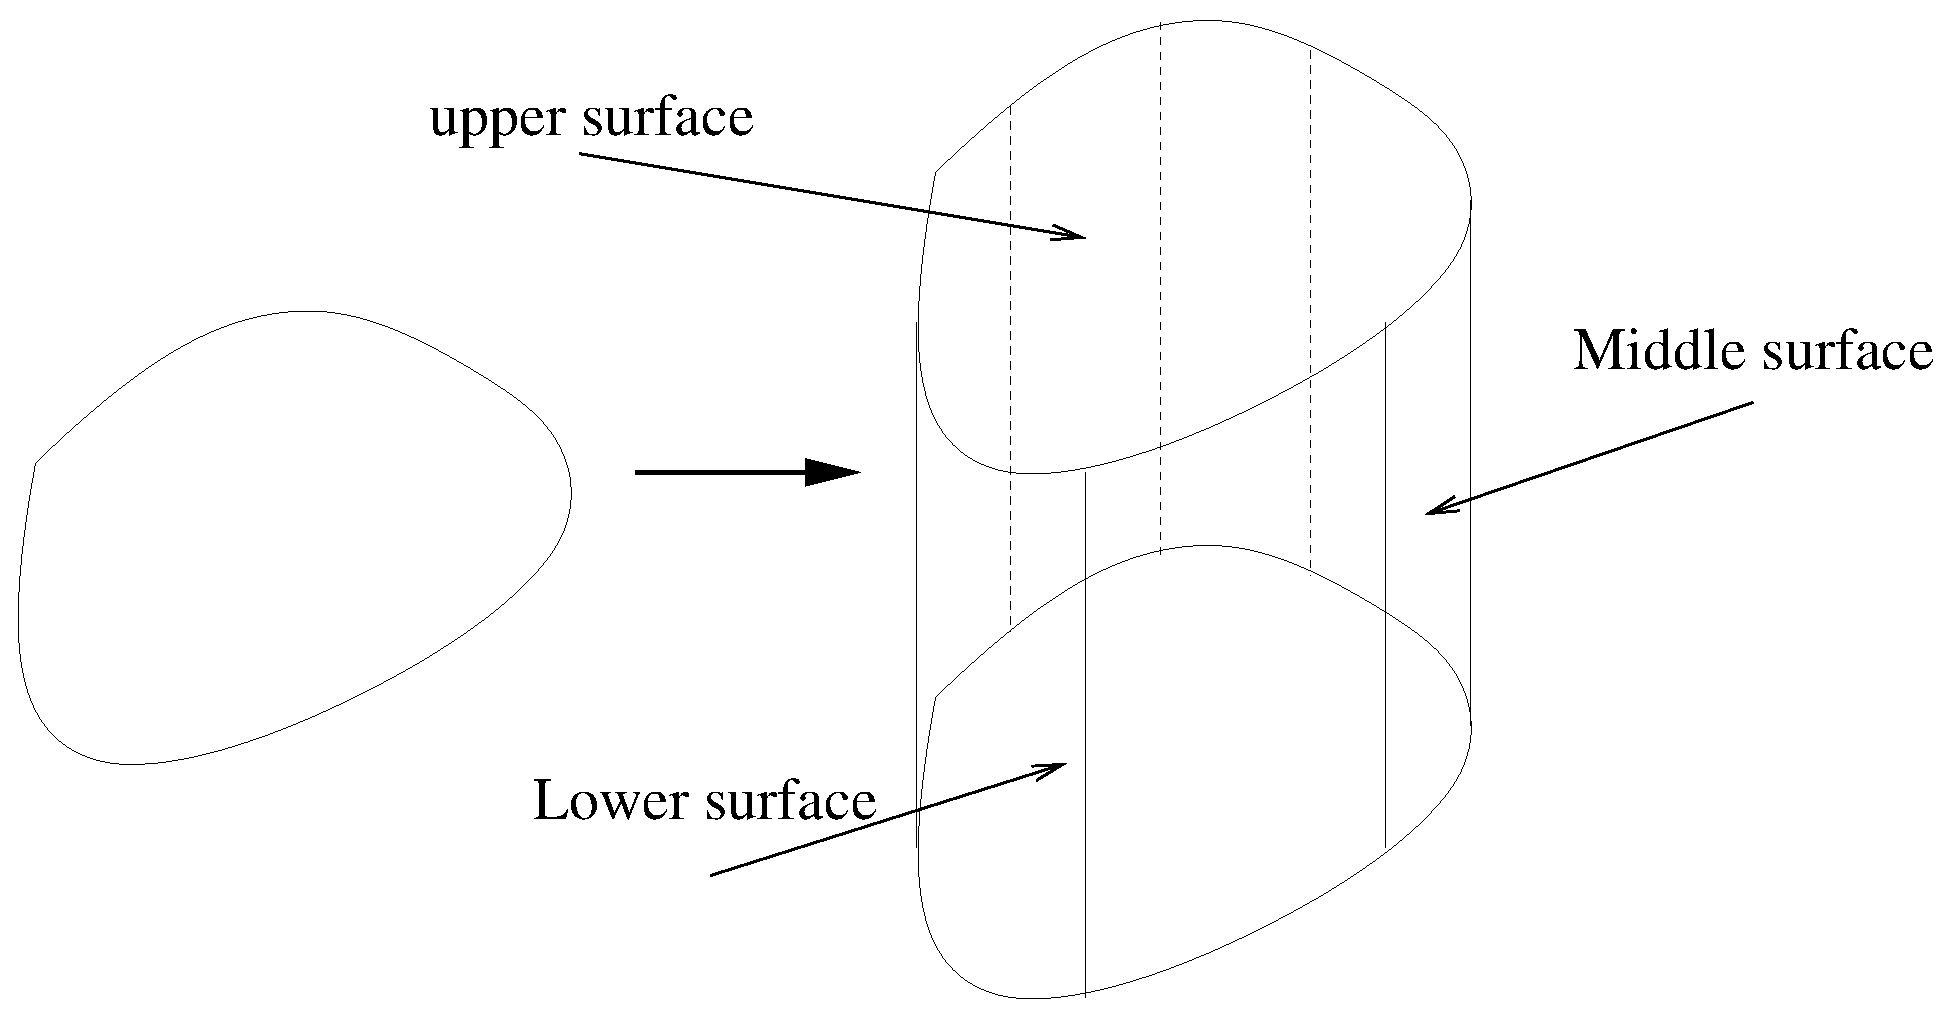
\includegraphics[height=5cm]{buillayermesh}
\caption{Example of Layer mesh in three dimension.}
\label{fig-layermeshextend}
\end{figure}

For a vertex of a two dimensional mesh $V_{i}^{2d} = (x_{i},y_{i})$, we introduce the number of associated vertices in the $z-$axis $M_{i}+1$.
We denote by $M$ the maximum of $M_{i}$ over the vertices of the two dimensional mesh. This value are called the number of layers
(if $\forall i, \; M_{i}=M$ then there are $M$ layers in the mesh of $\Omega_{3d}$). $V_{i}^{2d}$ generated $M+1$ vertices which are defined by
$$
\forall j=0, \ldots, M, \qquad  V_{i,j}^{3d} = ( x_{i}, y_{i}, \theta_{i}(z_{i,j})  ),
$$
where $(z_{i,j})_{j=0,\ldots,M}$ are the $M+1$ equidistant points on the interval $[zmin( V_{i}^{2d} ), zmax( V_{i}^{2d})]$:
\begin{eqnarray*}
z_{i,j} =  j \: \delta \alpha + zmin(V_{i}^{2d}), \qquad \delta \alpha= \frac{ zmax( V_{i}^{2d} ) - zmin( V_{i}^{2d}) }{M}.
\end{eqnarray*}
The function $\theta_{i}$, defined on  $[zmin( V_{i}^{2d} ), zmax( V_{i}^{2d} )]$, is given by
$$
\theta_{i}(z) = \left \{
\begin{array}{cl}
\theta_{i,0} & \mbox{if} \: z=zmin(V_{i}^{2d}), \\
\theta_{i,j} & \mbox{if} \: z \in ] \theta_{i,j-1}, \theta_{i,j}],\\
\end{array}
\right.
$$
with $(\theta_{i,j})_{j=0,\ldots,M_{i}}$ are the $M_{i}+1$ equidistant points on the interval $[zmin( V_{i}^{2d} ), zmax( V_{i}^{2d} )]$.\\

Set a triangle $K=(V_{i1}^{2d}$, $V_{i2}^{2d}$, $V_{i3}^{2d})$ of the two dimensional mesh.
$K$ is associated with a triangle on the upper surface (resp. on the lower surface) of layer mesh:
$( V_{i1,M}^{3d}, V_{i2,M}^{3d}, V_{i3,M}^{3d} )$ (resp. $( V_{i1,0}^{3d}, V_{i2,0}^{3d}, V_{i3,0}^{3d})$).

Also $K$ is associated with $M$ volume prismatic elements which are defined by
$$
\forall j=0,\ldots,M, \quad H_{j} = ( V_{i1,j}^{3d}, V_{i2,j}^{3d}, V_{i3,j}^{3d}, V_{i1,j+1}^{3d}, V_{i2,j+1}^{3d}, V_{i3,j+1}^{3d} ).
$$

Theses volume elements can have some merged point:
\begin{itemize}
\item 0 merged point : prism
\item 1 merged points : pyramid
\item 2 merged points : tetrahedra
\item 3 merged points : no elements
\end{itemize}

The elements with merged points are called degenerate elements. To obtain a mesh with tetrahedra, we decompose
the pyramid into two tetrahedra and the prism into three tetrahedra. These tetrahedra are obtained by cutting the quadrilateral
face of pyramid and prism with the diagonal which have the vertex with the maximum index (see \cite{hdrHecht} for the reaspn of this choice).\\

The triangles on the middle surface obtained with the decomposition of the volume prismatic elements are the triangles generated by the edges
on the border of the two dimensional mesh. The label of triangles on the border elements and tetrahedra are defined with the label of these
associated elements.\\


The arguments of \texttt{buildlayermesh} is a two dimensional mesh and the number of layers $M$.

The parameters of this command are:
\begin{description}
\item [\texttt{zbound  =}] [zmin,zmax] where zmin and zmax are functions expression. Theses functions define the lower surface mesh and upper mesh of surface mesh.
\item [\texttt{coef    =}] A function expression between [0,1]. This parameter is used to introduce degenerate element in mesh.
The number of associated points or vertex $V_{i}^{2d}$ is the integer part of $coef(V_{i}^{2d}) M$.
\item [\texttt{region  =}] This vector is used to initialized the region of tetrahedra. This vector contain  successive pair of  the  2d region number at index $2i$ and the corresponding    3d region number at index $2i+1$, like (\ref{eq.org.vector.change.label}).
become the
\item [\texttt{labelmid =}] This vector is used to initialized the 3d labels number  of the vertical face or mid face form the 2d
label number.   This vector contains  successive pair of the  2d label number
at index $2i$ and the corresponding   3d label number at index $2i+1$, like (\ref{eq.org.vector.change.label}).

\item [\texttt{labelup  =}] This vector is used to initialized the 3d label numbers  of the upper/top face form the 2d
region number.   This vector contains  successive pair of the  2d region number
at index $2i$ and the corresponding  3d label number at index $2i+1$, like (\ref{eq.org.vector.change.label}).

\item [\texttt{labeldown =}] Same as the previous case but for the lower/down face label .
\end{description}

Moreover, we also add post processing parameters that allow to moving the mesh. These parameters correspond to parameters
\texttt{transfo}, \texttt{facemerge} and \texttt{ptmerge} of the command line \texttt{movemesh}.

The vector \texttt{region}, \texttt{labelmid}, \texttt{labelup} and \texttt{labeldown} These vectors are composed of $n_{l}$ successive pairs of number $O_i,N_l$  where $n_{l}$ is the number (label or region)
that we want to get.

%%% Example a couper entre les differentes commandes
An example of this command line is given in \texttt{buildlayermesh.edp}.

\begin{example}[cube.idp]\index{cube}
\label{cube.idp}~
\bFF
load "medit"
load "msh3"
@func @mesh3 Cube(int[int] & NN,real[int,int] &BB ,int[int,int] & L)
{
  //  first  build the 6 faces of the hex.
  @real x0=BB(0,0),x1=BB(0,1);
  @real y0=BB(1,0),y1=BB(1,1);
  @real z0=BB(2,0),z1=BB(2,1);

  @int nx=NN[0],ny=NN[1],nz=NN[2];
  @mesh Thx = square(nx,ny,[x0+(x1-x0)*x,y0+(y1-y0)*y]);

  @int[@int] rup=[0,L(2,1)],  rdown=[0,L(2,0)],
    rmid=[1,L(1,0),  2,L(0,1),  3, L(1,1),  4, L(0,0) ];
  @mesh3 Th=buildlayers(Thx,nz,   zbound=[z0,z1],
                       labelmid=rmid,   labelup = rup,
                       labeldown = rdown);

  @return Th;
}
\eFF

The unit cube example:
\bFF
 @include "Cube.idp"
 @int[int]  NN=[10,10,10]; //  the number of step in each  direction
 @real [int,int]  BB=[[0,1],[0,1],[0,1]]; // bounding box
 @int [int,int]  L=[[1,2],[3,4],[5,6]]; // the label of the 6 face left,right,
//  front, back, down, right
@mesh3 Th=Cube(NN,BB,L);
@medit("Th",Th); // see figure \ref{figs-cube}
\eFF
\end{example}


The cone example (an axisymtric mesh on a triangle with degenerateness).
\begin{example}[cone.edp]\index{cone}~
\bFF
@load "msh3"
@load "medit"
// cone using buildlayers with a triangle
@real RR=1,HH=1;
@border Taxe(t=0,HH){x=t;y=0;label=0;};
@border Hypo(t=1,0){x=HH*t;y=RR*t;label=1;};
@border Vert(t=0,RR){x=HH;y=t;label=2;};
@int nn=10;   real h= 1./nn;
@mesh Th2=buildmesh(  Taxe(HH*nn)+ Hypo(sqrt(HH*HH+RR*RR)*nn) + Vert(RR*nn) ) ;
@plot(Th2,wait=1); // the 2d mesh

@int MaxLayersT=(int(2*pi*RR/h)/4)*4;// number of layers
@real zminT = 0, zmaxT = 2*pi; // height $2*pi$
@func fx= y*cos(z); @func fy= y*sin(z); @func fz= x;
@int[i@nt] r1T=[0,0], r2T=[0,0,2,2], r4T=[0,2];
// trick  function:
@func deg= max(.01,y/max(x/HH,0.4) /RR); // the function defined the proportion
// of number layer close to axis with reference MaxLayersT
@mesh3 Th3T=buildlayers(Th2,coef=  deg, MaxLayersT,
           zbound=[zminT,zmaxT],transfo=[fx,fy,fz],
           facemerge=0, region=r1T, labelmid=r2T);
medit("cone",Th3T); // see figure \ref{figs-cone}
\eFF
\end{example}


\twoplot[height=8cm]{cube}{cone}{the mesh of a  cube made with cube.edp \label{figs-cube}}
{the mesh of a cone made with cone.edp \label{figs-cone}}



\index{buildlayers}
\begin{example}[buildlayermesh.edp]
\label{buildlayermesh}~
\bFF

// file buildlayermesh.edp

load "msh3"
load "tetgen"


// Test 1

@int C1=99, C2=98; // could be anything
@border C01(t=0,pi){ x=t;  y=0;      label=1;}
@border C02(t=0,2*pi){ x=pi; y=t;  label=1;}
@border C03(t=0,pi){ x=pi-t;  y=2*pi;    label=1;}
@border C04(t=0,2*pi){ x=0;    y=2*pi-t; label=1;}

@border C11(t=0,0.7){ x=0.5+t;  y=2.5;      label=C1;}
@border C12(t=0,2){ x=1.2;    y=2.5+t;  label=C1;}
@border C13(t=0,0.7){ x=1.2-t;  y=4.5;     label=C1;}
@border C14(t=0,2){ x=0.5;    y=4.5-t; label=C1;}

@border C21(t=0,0.7){ x= 2.3+t;     y=2.5;  label=C2;}
@border C22(t=0,2){        x=3;   y=2.5+t;  label=C2;}
@border C23(t=0,0.7){   x=3-t;     y=4.5;  label=C2;}
@border C24(t=0,2){       x=2.3;   y=4.5-t; label=C2;}

@mesh Th=@buildmesh(    C01(10)+C02(10)+ C03(10)+C04(10)
                    + C11(5)+C12(5)+C13(5)+C14(5)
                    + C21(-5)+C22(-5)+C23(-5)+C24(-5));

@mesh Ths=@buildmesh(    C01(10)+C02(10)+ C03(10)+C04(10)
                    + C11(5)+C12(5)+C13(5)+C14(5) );

// construction of a box with one hole and two regions
@func zmin=0.;
@func zmax=1.;
@int MaxLayer=10;

@func XX = x*cos(y);
@func YY = x*sin(y);
@func ZZ = z;

@int[int] r1=[0,41], r2=[98,98,  99,99, 1,56];
@int[int] r3=[4,12];    //  The triangles of uppper surface mesh
// generated by the triangle in the 2D region of mesh Th of label 4 as label 12.
@int[int] r4=[4,45];    //  The triangles of lower surface mesh
// generated by the triangle in the 2D region of mesh Th of label 4 as label 45.

@mesh3 Th3=@buildlayers( Th, MaxLayer, zbound=[zmin,zmax], region=r1,
                labelmid=r2, labelup = r3, labeldown = r4 );
@savemesh(Th3,"box2region1hole.mesh");
// construction of a sphere with TetGen
@func XX1 = cos(y)*sin(x);
@func YY1 = sin(y)*sin(x);
@func ZZ1 = cos(x);
@string test="paACQ";
cout << "test=" << test << endl;
@mesh3 Th3sph=@tetgtransfo(Ths,transfo=[XX1,YY1,ZZ1],switch=test,nbofregions=1,
                           regionlist=domain);
@savemesh(Th3sph,"sphere2region.mesh");

\eFF
\end{example}

\subsection{Meshing examples}


\begin{example}[lac.edp]
// file "lac.edp"
\bFF
@load ``msh3''
@int nn=5;
@border cc(t=0,2*pi){x=cos(t);y=sin(t);label=1;}
@mesh Th2 = @buildmesh(cc(100));
@fespace Vh2(Th2,P2);
Vh2 ux,uy,p2;
@int[int] rup=[0,2], rdlow=[0,1], rmid=[1,1,2,1,3,1,4,1];
@func zmin = 2-sqrt(4-(x*x+y*y));
@func zmax = 2-sqrt(3.);

@mesh3 Th = @buildlayers(Th2,nn,
  coeff = max((zmax-zmin)/zmax, 1./nn),
  zbound=[zmin,zmax],
  labelmid=rmid;
  labelup=rup;
  labeldown=rlow);
@savemesh(Th,''Th.meshb'');
@exec(``medit Th; Th.meshb'');
\eFF
\end{example}

\begin{example}[tetgenholeregion.edp]
\bFF
// file ``tetgenholeregion.edp''
@load "msh3''
@load "tetgen"

@mesh Th=square(10,20,[x*pi-pi/2,2*y*pi]);  //  $]\frac{-pi}{2},\frac{-pi}{2}[\times]0,2\pi[ $
//  a parametrization of a sphere
@func f1 =cos(x)*cos(y);
@func f2 =cos(x)*sin(y);
@func f3 = sin(x);
//  partiel derivative of the parametrization DF
@func f1x=sin(x)*cos(y);
@func f1y=-cos(x)*sin(y);
@func f2x=-sin(x)*sin(y);
@func f2y=cos(x)*cos(y);
@func f3x=cos(x);
@func f3y=0;
// $  M = DF^t DF $
@func m11=f1x^2+f2x^2+f3x^2;
@func m21=f1x*f1y+f2x*f2y+f3x*f3y;
@func m22=f1y^2+f2y^2+f3y^2;

@func perio=[[4,y],[2,y],[1,x],[3,x]];
@real hh=0.1;
@real vv= 1/square(hh);
verbosity=2;
Th=@adaptmesh(Th,m11*vv,m21*vv,m22*vv,IsMetric=1,periodic=perio);
Th=@adaptmesh(Th,m11*vv,m21*vv,m22*vv,IsMetric=1,periodic=perio);
@plot(Th,wait=1);

verbosity=2;

// construction of the surface of spheres
@real Rmin  = 1.;
@func f1min = Rmin*f1;
@func f2min = Rmin*f2;
@func f3min = Rmin*f3;

@mesh3 Th3sph = @movemesh23(Th,transfo=[f1min,f2min,f3min]);

@real Rmax  = 2.;
@func f1max = Rmax*f1;
@func f2max = Rmax*f2;
@func f3max = Rmax*f3;

@mesh3 Th3sph2 = @movemesh23(Th,transfo=[f1max,f2max,f3max]);

cout << "addition" << endl;
@mesh3 Th3 = Th3sph+Th3sph2;

@real[int] domain2 = [1.5,0.,0.,145,0.001,0.5,0.,0.,18,0.001];
cout << "==============================" << endl;
cout << " tetgen call without hole " << endl;
cout << "==============================" << endl;
@mesh3 Th3fin = @tetg(Th3,switch="paAAQYY",nbofregions=2,regionlist=domain2);
cout << "=============================" << endl;
cout << "finish tetgen call without hole" << endl;
cout << "=============================" << endl;
savemesh(Th3fin,"spherewithtworegion.mesh");

@real[int] hole = [0.,0.,0.];
@real[int] domain = [1.5,0.,0.,53,0.001];
cout << "=============================" << endl;
cout << "  tetgen call with hole   " << endl;
cout << "=============================" << endl;
@mesh3 Th3finhole=@tetg(Th3,switch="paAAQYY",nbofholes=1,holelist=hole,
nbofregions=1,regionlist=domain);
cout << "=============================" << endl;
cout << "finish tetgen call with hole   " << endl;
cout << "=============================" << endl;
@savemesh(Th3finhole,"spherewithahole.mesh");
\eFF
\end{example}

\subsubsection{Build a 3d mesh of a cube with a balloon}
\label{cube-ballon}

First the \texttt{MeshSurface.idp} file to build boundary mesh of a Hexaedra and of a Sphere.


\bFF
@func @mesh3 SurfaceHex(@int[@int] & N,@real[@int,@int] &B ,@int[@int,@int] & L,@int orientation)
{
    @real x0=B(0,0),x1=B(0,1);
    @real y0=B(1,0),y1=B(1,1);
    @real z0=B(2,0),z1=B(2,1);

    @int nx=N[0],ny=N[1],nz=N[2];

    @mesh Thx = square(ny,nz,[y0+(y1-y0)*x,z0+(z1-z0)*y]);
    @mesh Thy = square(nx,nz,[x0+(x1-x0)*x,z0+(z1-z0)*y]);
    @mesh Thz = square(nx,ny,[x0+(x1-x0)*x,y0+(y1-y0)*y]);

    @int[int] refx=[0,L(0,0)],refX=[0,L(0,1)];//  Xmin, Ymax faces labels renumbering
    @int[int] refy=[0,L(1,0)],refY=[0,L(1,1)];//  Ymin, Ymax faces labesl renumbering
    @int[int] refz=[0,L(2,0)],refZ=[0,L(2,1)];//  Zmin, Zmax faces labels renumbering

    @mesh3 Thx0 = movemesh23(Thx,transfo=[x0,x,y],orientation=-orientation,label=refx);
    @mesh3 Thx1 = movemesh23(Thx,transfo=[x1,x,y],orientation=+orientation,label=refX);
    @mesh3 Thy0 = movemesh23(Thy,transfo=[x,y0,y],orientation=+orientation,label=refy);
    @mesh3 Thy1 = movemesh23(Thy,transfo=[x,y1,y],orientation=-orientation,label=refY);
    @mesh3 Thz0 = movemesh23(Thz,transfo=[x,y,z0],orientation=-orientation,label=refz);
    @mesh3 Thz1 = movemesh23(Thz,transfo=[x,y,z1],orientation=+orientation,label=refZ);
    @mesh3 Th= Thx0+Thx1+Thy0+Thy1+Thz0+Thz1;
    @return Th;
}


@func @mesh3 Sphere(@real R,@real h,@int L,@int orientation)
{
  @mesh  Th=square(10,20,[x*pi-pi/2,2*y*pi]);  //  $]\frac{-pi}{2},frac{-pi}{2}[\times]0,2\pi[ $
  //  a parametrization of a sphere
  @func f1 =cos(x)*cos(y);
  @func f2 =cos(x)*sin(y);
  @func f3 = sin(x);
  //    partiel derivative
  @func f1x=sin(x)*cos(y);
  @func f1y=-cos(x)*sin(y);
  @func f2x=-sin(x)*sin(y);
  @func f2y=cos(x)*cos(y);
  @func f3x=cos(x);
  @func f3y=0;
  // the metric on the sphere  $  M = DF^t DF $
  @func m11=f1x^2+f2x^2+f3x^2;
  @func m21=f1x*f1y+f2x*f2y+f3x*f3y;
  @func m22=f1y^2+f2y^2+f3y^2;

  @func perio=[[4,y],[2,y],[1,x],[3,x]];  // to store the periodic condition

  @real hh=h/R;// hh  mesh size on unite sphere
  @real vv= 1/square(hh);
  Th=adaptmesh(Th,m11*vv,m21*vv,m22*vv,IsMetric=1,periodic=perio);
  Th=adaptmesh(Th,m11*vv,m21*vv,m22*vv,IsMetric=1,periodic=perio);
  Th=adaptmesh(Th,m11*vv,m21*vv,m22*vv,IsMetric=1,periodic=perio);
  Th=adaptmesh(Th,m11*vv,m21*vv,m22*vv,IsMetric=1,periodic=perio);
  @int[@int] ref=[0,L];

  @mesh3  ThS= movemesh23(Th,transfo=[f1*R,f2*R,f3*R],orientation=orientation,refface=ref);
  @return ThS;
}

\eFF

The test of the two functions and the call to \texttt{tetgen} mesh generator
\bFF
 load "tetgen"
 @include "MeshSurface.idp"
    @real hs = 0.1;  // mesh size on sphere
    @int[int]  N=[20,20,20];
    @real [int,int]  B=[[-1,1],[-1,1],[-1,1]];
    @int [int,int]  L=[[1,2],[3,4],[5,6]];
    @mesh3 ThH = SurfaceHex(N,B,L,1);
    @mesh3 ThS =Sphere(0.5,hs,7,1); // "gluing" surface meshs to tolat boundary meshes

    @mesh3 ThHS=ThH+ThS;
    @savemesh(ThHS,"Hex-Sphere.mesh");
    @exec("ffmedit Hex-Sphere.mesh;rm Hex-Sphere.mesh");// see \ref{figs-Hex-Sphere}

    @real voltet=(hs^3)/6.;
    @cout << " voltet = " << voltet << endl;
    @real[int] domaine = [0,0,0,1,voltet,0,0,0.7,2,voltet];

    @mesh3 Th = tetg(ThHS,switch="pqaAAYYQ",nbofregions=2,regionlist=domaine);
    @medit("Cube-With-Ball",Th);// see \ref{Cube-With-Ball}

\eFF
\twoplot[height=8cm]{Hex-Sphere}{Cube-With-Ball}{The surface mesh of the Hex with internal Sphere \label{figs-Hex-Sphere}}
{The tet mesh of the cube with internal ball\label{figs-Cube-With-Ball}}

\subsection{The output solution formats .sol and .solb}
With the keyword savesol, we can store a scalar functions, a scalar FE functions,
a vector fields, a vector FE fields, a symmetric tensor and a symmetric FE tensor..
Such format is used in medit.

\paragraph{extension file .sol}
\def\Int#1{ {\tt(I)} #1}
\def\Loop#1#2{{\bf\Large(}\,#1\,{\bf\Large{,\,\,}}\,#2\,{\bf\Large)}}

The first two lines of the file are
\small
\begin{itemize}
\item {\tt MeshVersionFormatted 0}
\end{itemize}
\normalsize

\small
\begin{itemize}
\item {\tt Dimension}
  \Int{dim}
\end{itemize}

The following fields begin with one of the following keyword:
SolAtVertices, SolAtEdges, SolAtTriangles, SolAtQuadrilaterals,
SolAtTetrahedra, SolAtPentahedra, SolAtHexahedra.

In each field, we give then in the next line the number of elements in the solutions
(SolAtVertices: number of vertices, SolAtTriangles: number of triangles, ...). In other lines, we give
 the number of solutions , the type of solution (1: scalar, 2: vector, 3: symmetric tensor).
 And finally,  we give the values of the solutions on the elements.

The file must be ended with the keyword End.

The real element of symmetric tensor
\begin{eqnarray}
\label{savesol.def.symtensor}
ST^{3d}=\left(
\begin{array}{ccc}
ST_{xx}^{3d} & ST_{xy}^{3d} & ST_{xz}^{3d}\\
ST_{yx}^{3d} & ST_{yy}^{3d} & ST_{yz}^{3d} \\
ST_{zx}^{3d} & ST_{zy}^{3d} & ST_{zz}^{3d}
\end{array}
\right)
\qquad \qquad
ST^{2d}= \left(
\begin{array}{cc}
ST_{xx}^{2d} & ST_{xy}^{2d} \\
ST_{yx}^{2d} & ST_{yy}^{2d}
\end{array}
\right)
\end{eqnarray}
stored in the extension .sol are respectively $ST_{xx}^{3d}, ST_{yx}^{3d}, ST_{yy}^{3d}, ST_{zx}^{3d}, ST_{zy}^{3d}, ST_{zz}^{3d}$
and  $ST_{xx}^{2d}, ST_{yx}^{2d}, ST_{yy}^{2d}$

An example of field with the keyword SolAtTetrahedra:
\small
\begin{itemize}
\item {\tt{SolAtTetrahedra}}\\
  \Int{NbOfTetrahedrons}
  {\tt \obeylines
  $ \mathtt{ \quad nbsol \quad typesol^1 \quad ... \quad typesol^n }  $
  $\left(\left(\left( \mathtt{U}_{ij}^k, \quad \forall i \in \{1,...,\mathtt{nbrealsol}^k\}\right), %
\quad \forall k \in \{1,...\mathtt{nbsol}\}\right) %
 \quad \forall j \in \{1,...,\mathtt{NbOfTetrahedrons}\}\right)$
 }
\end{itemize}
where
\begin{itemize}
\item {\tt  nbsol} is an integer equal to the number of solutions
\item $\mathtt{  typesol^k}$, type of the solution  number $ k$, is
  \begin{itemize}
   \item $\mathtt{typesol^k = 1}$ the solution {\tt k} is scalar.
   \item $\mathtt{typesol^k = 2}$ the solution {\tt k} is vectorial.
   \item $\mathtt{typesol^k = 3}$ the solution {\tt k} is a symmetric tensor or symmetric matrix.
   \end{itemize}
\item  $\mathtt{  nbrealsol^k}$ number of real to discribe solution number $k$ is
  \begin{itemize}
   \item $\mathtt{nbrealsol^k = 1}$ the solution {\tt k} is scalar.
   \item $\mathtt{nbrealsol^k = dim}$ the solution {\tt k} is vectorial ($dim$ is the dimension of the solution).
   \item $\mathtt{nbrealsol^k = dim*(dim+1)/2}$ the solution {\tt k} is a symmetric tensor or symmetric matrix.
   \end{itemize}
\item  {\tt U$_{ij}^k$} is a real equal to the value of the component  $i$ of the solution  $k$ at tetrahedra $j$
on the associated mesh.
\end{itemize}

This field is written with the notation of Section \ref{meshformatfile.mesh}.
The format .solb is the same as format .sol but in binary (read/write is faster, storage is less).

A real scalar functions $f1$, a vector fields $\Phi=[\Phi1,\Phi2,\Phi3]$ and a symmetric tensor $ST^{3d}$
(\ref{savesol.def.symtensor}) at the vertices of the three dimensional mesh Th3 is stored in the file "f1PhiTh3.sol" using
\index{savesol!order=}
\bFF
@savesol("f1PhiST3dTh3.sol",Th3, $f1$, [$\Phi$1, $\Phi$2, $\Phi$3], VV3, order=1);
\eFF
where $VV3=[ ST_{xx}^{3d}, ST_{yx}^{3d}, ST_{yy}^{3d}, ST_{zx}^{3d}, ST_{zy}^{3d}, ST_{zz}^{3d}]$.
For a two dimensional mesh Th, A real scalar functions $f2$, a vector fields $\Psi=[\Psi1,\Psi2]$ and a symmetric tensor $ST^{2d}$
(\ref{savesol.def.symtensor}) at triangles is stored in the file "f2PsiST2dTh3.solb" using
\bFF
@savesol("f2PsiST2dTh3.solb",Th, $f2$, [$\Psi$1, $\Psi$2], VV2, order=0);
\eFF
where $VV2=[ST_{xx}^{2d}, ST_{yx}^{2d}, ST_{yy}^{2d}]$
The arguments of \texttt{savesol} functions are the name of a file, a mesh and solutions. These arguments must be given in this order.

The parmameters of this keyword are
\begin{description}
%\item [\texttt{nbscalar =}] number of scalar solutions ($nbs$).
%\item [\texttt{scalar   =}]  \texttt{[$f_{1}$, $f_{2}$, $f_{3}$, ..., $f_{nbs}$]} set the $nbs$ scalar solutions.
%\item [\texttt{nbvector =}] number of vector solutions ($nbv$).
%\item [\texttt{nbsymtensor =}] number of symmetric tensor solutions ($nbst$).
%\item [\texttt{vector    =}] set the real element of $nbv$ vector solutions.
%\item [\texttt{symtensor =}] set the real element of $nbst$ symmetric tensor solutions.
\item [\texttt{order =}] 0 is the solution is given at the center of gravity of elements.
1 is the solution is given at the vertices of elements.
\end{description}

%%In two dimensional case for vector solutions $v^{j}=(v^{j}_{x},v^{j}_{y}), \quad j=1,\ldots nbv$, the parameter \texttt{vector} is equal to
%%\texttt{[$v_{x}^{1}$, $v_{y}^{1}$, ..., $v_{x}^{nbv}$, $v_{y}^{nbv}$]}.

%%In two dimensional case for symtensor solutions $st^{j}= \left (
%%\begin{array}{ccc}
%%st_{xx}^{j} & st_{xy}^{j} & st_{xz}^{j} \\
%%st_{yx}^{j} & st_{yy}^{j} & st_{yz}^{j} \\
%%st_{zx}^{j} & st_{zy}^{j} & st_{zz}^{j}
%%\end{array}
%%\right) \quad j=1,\ldots nbst$, the parameter \texttt{vector} is equal to
%%\texttt{[ $st_{xx}^{1}$, $st_{yx}^{1}$, $st_{yy}^{1}$, ..., $st_{xx}^{nbst}$, $st_{yx}^{nbst}$, $st_{yy}^{nbst}$]}.
%%\item [\texttt{symtensor =}] \texttt{[ $st_{xx}^{1}$, $st_{yx}^{1}$, $st_{yy}^{1}$, ..., $st_{xx}^{nbst}$, $st_{yx}^{nbst}$, $st_{yy}^{nbst}$]}
%%set the real element of $nbst$ symmetric tensor solutions  $st^{j}=(st^{j}_{x},st^{j}_{y}), \quad j=1,\ldots nbst$.
%%Three dimensional case:
%%\item [\texttt{vector   =}] \texttt{[$f_{x}^{1}$, $f_{y}^{1}$, $f_{z}^{1}$, ..., $f_{x}^{nbv}$, $f_{y}^{nbv}$, $f_{z}^{nbv}$  ]}
%%set the $nbv$ vector solutions.
%%\item [\texttt{symtensor   =}] \texttt{[ $f_{xx}^{1}$, $f_{yx}^{1}$, $f_{yy}^{1}$, $f_{zx}^{1}$, $f_{zy}^{1}$, $f_{zz}^{1}$,
%%..., $f_{xx}^{nbst}$, $f_{yx}^{nbst}$, $f_{yy}^{nbst}$, $f_{zx}^{nbst}$, $f_{zy}^{nbst}$, $f_{zz}^{nbst}$ ]}
%%set the $nbst$ symmetric tensor solutions.

In the file, solutions are stored in this order : scalar solutions, vector solutions and finally symmetric
tensor solutions.

\subsection{medit}

The keyword medit allows to dipslay a mesh alone or a mesh and one or several functions defined on the mesh using the Pascal Frey's freeware medit.
Medit opens its own window and uses OpenGL extensively.
Naturally to use this command  medit must be installed.
%%This command allow to represent one solution.

A vizualisation with medit of scalar solutions $f1$ and $f2$ continuous, piecewise linear and known at the vertices of the mesh Th is obtained using
\bFF
@medit("sol1 sol2",Th, $f1$, $f2$, order=1);
\eFF
The first plot  named ``sol1'' display f1. The second plot names ``sol2'' display f2.

The arguments of function \texttt{medit} are the name of the differents scenes (separated by a space) of medit, a mesh and solutions.
Each solution is associated with one scene. The scalar, vector and symmetric tensor solutions are specified in the format described in the section dealing with the keyword \texttt{savesol}.

%%These arguments must be given in this order.

The parameters of this command line are
\begin{description}
%%\item [\texttt{solution =}] An integer parameter. This parameter is equal to 0 if there is no solution to display and otherwise is equal to 1.
\item [\texttt{order =}] 0 is the solution is given at the center of gravity of elements.
1 is the solution is given at the vertices of elements.
\index{medit!order=}
\index{medit!meditff=}
\item [\texttt{meditff =}] set the name of execute command of medit. By default, this string is medit.
\index{medit!save=}
\item [\texttt{save =}] set the name of a file .sol or .solb to save solutions.
%%\item [\texttt{scalar =}] set the scalar solutions to display.
%%two dimensional case:
%%\item [\texttt{vector =}] set the vector field solution $v=(v_{x},v_{y})$. This parameter is equal to \texttt{[$v_{x}$,$v_{y}$]}.
%%\item [\texttt{symtensor =}]  set the symmetric tensor solution
%%$
%%f= \left (
%%\begin{array}{cc}
%%f_{xx} & f_{xy} \\
%%f_{yx} & f_{yy}
%%\end{array}
%%\right)
%%$. This parmameter is equal to \texttt{[$f_{xx}$, $f_{yx}$, $f_{yy}$]}
%%three dimensional case:
%%\item [\texttt{vector =}] set the vector field solution $v=(v_{x},v_{y},v_{z})$. This parameter is equal to  \texttt{[$v_{x}$,$v_{y}$,$v_{z}$]}.
%%\item [\texttt{symtensor =}] set the symmetric tensor solution
%%$
%%f= \left (
%%\begin{array}{ccc}
%%f_{xx} & f_{xy} & f_{xz}\\
%%f_{yx} & f_{yy} & f_{yz} \\
%%f_{zx} & f_{zy} & f_{zz}
%%\end{array}
%%\right)
%%$. This parameter is equal to \texttt{[$f_{xx}$, $f_{yx}$, $f_{yy}$, $f_{zx}$, $f_{zy}$, $f_{zz}$]}
\end{description}

This command line allows also to represent two differents meshes and solutions on them in the same windows.
The nature of solutions must be the same. Hence, we can vizualize in the same window the different
domains in a domain decomposition method for instance. A vizualisation with medit of scalar solutions $h1$ and $h2$
at vertices of the mesh Th1 and Th2 respectively  are obtained using
\bFF
@medit("sol2domain",Th1, $h1$, Th2, $h2$, order=1);
\eFF

\begin{example}[meditddm.edp]
\bFF
// meditddm.edp
@load "medit"


// Initial Problem:
//Resolution of the following EDP:
//$- \Delta u_s = f$ on   $\Omega =\{ (x,y) |  1 \leq sqrt(x^2+y^2) \geq 2 \}$\hfilll
//$- \Delta u_1 = f1$ on  $\Omega_{1}=\{ (x,y) |  0.5 \leq sqrt(x^2+y^2) \geq 1. \}$\hfilll
//$u = 1$ on $\Gamma$  +  Null Neumman condition on $\Gamma_{1}$ and on $\Gamma_{2}$\hfilll
//We find the solution $u$ in solving two EDP defined on domain $\Omega$ and $\Omega_{1}$\hfilll
//This solution is visualize with medit

verbosity=3;

@border Gamma(t=0,2*pi){x=cos(t); y=sin(t); label=1;};
@border Gamma1(t=0,2*pi){x=2*cos(t); y=2*sin(t); label=2;};
@border Gamma2(t=0,2*pi){x=0.5*cos(t); y=0.5*sin(t); label=3;};

// construction of mesh of domain $\Omega$
@mesh Th=buildmesh(Gamma1(40)+Gamma(-40));

@fespace Vh(Th,P2);
@func f=sqrt(x*x+y*y);
Vh us,v;
@macro Grad2(us) [dx(us),dy(us)]  // EOM

@problem Lap2dOmega(us,v,init=false)=int2d(Th)(Grad2(v)' *Grad2(us)) 
   - int2d(Th)(f*v)+on(1,us=1) ;

//   Definition of EDP defined on the domain $\Omega$\hfilll
// $- \Delta u_s = f_1$ on $\Omega_{1}$,     $u_s = 1$ on $\Gamma_1$, $\frac{\partial u_s}{\partial n} =0 $ on $\Gamma_{2}$\hfilll
Lap2dOmega;

// construction of mesh of domain $\Omega_{1}$
@mesh Th1=buildmesh(Gamma(40)+Gamma2(-40));

@fespace Vh1(Th1,P2);
@func f1=10*sqrt(x*x+y*y);
Vh1 u1,v1;
@macro Grad21(u1) [dx(u1),dy(u1)]  // EOM

@problem Lap2dOmega1(u1,v1,init=false)=int2d(Th1)(Grad21(v1)' *Grad21(u1)) 
            - int2d(Th1)(f1*v1)+on(1,u1=1) ;
//   Resolution of EDP defined on the domain $\Omega_{1}$\hfilll
// $- \Delta u_1 = f_1$ on $\Omega_{1}$,     $u-1 = 1$ on $\Gamma_1$, $\frac{\partial u_1}{\partial n} =0 $ on $\Gamma_{2}$\hfilll
Lap2dOmega1;

// vizualisation of solution of the initial problem
@medit("solution",Th,us,Th1,u1,order=1,save="testsavemedit.solb");	
\eFF
\end{example}

\begin{example}[StockesUzawa.edp]
\bFF
//  signe of pressure is correct
@assert(version>1.18);
@real s0=clock();
@mesh Th=square(10,10);
@fespace Xh(Th,P2),Mh(Th,P1);
@Xh u1,u2,v1,v2;
@Mh p,q,ppp;


@varf bx(u1,q) = @int2d(Th)( (dx(u1)*q));
@varf by(u1,q) = @int2d(Th)( (dy(u1)*q));
@varf a(u1,u2)=  @int2d(Th)(  dx(u1)*dx(u2) + dy(u1)*dy(u2) )
                    +  @on(1,2,4,u1=0)  +  @on(3,u1=1) ;

Xh bc1; bc1[] = a(0,Xh);
Xh b;

@matrix A= a(Xh,Xh,solver=CG);
@matrix Bx= bx(Xh,Mh);
@matrix By= by(Xh,Mh);
Xh bcx=1,bcy=0;

@func @real[@int] divup(@real[@int] & pp)
{
  @int verb=verbosity;
   verbosity=0;
   b[]  = Bx'*pp; b[] += bc1[] .*bcx[];
   u1[] = A^-1*b[];
   b[]  = By'*pp; b[] += bc1[] .*bcy[];
   u2[] = A^-1*b[];
   ppp[] =   Bx*u1[];
   ppp[] +=  By*u2[];
   verbosity=verb;
   @return ppp[] ;
};
p=0;q=0;u1=0;v1=0;


@LinearCG(divup,p[],q[],eps=1.e-6,nbiter=50);

divup(p[]);

@plot([u1,u2],p,wait=1,value=true,coef=0.1);
@medit("velocity pressure",Th,[u1,u2],p,order=1);
\eFF
\end{example}


%%% frey et al. software


\subsection{Mshmet}
\label{sec:mshmet}

Mshmet is a software developped by P. Frey that allows to compute an anisotropic metric based on solutions (i.e. Hessian-based). This sofware can return also an isotropic metric. Moreover,  mshmet can construct also a metric suitable for level sets interface capturing. The solution can be defined on 2D or 3D structured/unstructured meshes. For example, the solution can be an error estimate of a FE solutions.

%%Error estimate for 2d and 3d unstructured meshes.
%%Compute anisotropic metric based on solution variations (i.e. Hessian-based).
%%One option allows to construct a metric suitable for level set interface capturing.

Solutions for mshmet are given as an argument. The solution can be a func, a vector func, a symmetric tensor, a FE func, a FE vector func and a FE symmetric tensor. The symmetric tensor argument is defined as this type of data for datasol argument. This software accepts more than one solution.

For example, the metric $M$ computed with mshmet  for the solution $u$ defined on the mesh $Th$ is obtained by writing.
\bFF
fespace Vh(Th,P1);
Vh u; // a scalar FE func
real[int] M = mshmet(Th,u);
\eFF

The parameters of the keyword mshmet are :
\begin{itemize}\parskip=0cm
%\item	\texttt{metric =  <3KN_IdE>} 
\item	\texttt{normalization =  <b>} do a normalisation of all solution in $[0,1]$.
\item	\texttt{aniso =  <b>} build aniso metric if 1 ( delault 0: iso) 
\item	\texttt{levelset =  <b>} {build metric for level set method (default: false)}
\item	\texttt{verbosity =  <l>}
\item	\texttt{nbregul =  <l>} number of regularization's iteration of solutions given (default 0).
\item	\texttt{hmin =  <d>}
\item	\texttt{hmax =  <d>}
\item	\texttt{err =  <d>} level of error. 
\item	\texttt{width =  <d>} the width 
\item \texttt{metric}= a vector of double. This vector contains an initial metric given to mshmet. The structure of the metric vector is described in the next paragraph.

\item \texttt{loptions}=]a vector of integer of size 7. This vector contains the integer parameters of mshmet(for expert only).
\begin{itemize} \item loptions(0): normalization (default 1).
\item loptions(1): isotropic parameters (default 0). 1 for isotropic metric results otherwise 0.
\item loptions(2): level set parameters (default 0). 1 for building level set metric otherwise 0.
\item loptions(3): debug parameters (default 0). 1 for turning on debug mode otherwise 0.
\item loptions(4): level of verbosity (default 10).
\item loptions(5): number of regularization's iteration of solutions given (default 0). 
\item loptions(6): previously metric parameter (default 0). 1 for using previous metric otherwise 0.
\end{itemize}

\item \texttt{doptions}= a vector of double of size 4. This vector contains the real parameters of mshmet (for expert only).
\begin{itemize}
\item doptions(0):  hmin : min size parameters  (default 0.01).
\item doptions(1):  hmax : max size parameters (default 1.0).
\item doptions(2):  eps : tolerance parameters ( default 0.01).
\item doptions(2):  width : relative width for Level Set ($0<w<1$) ( default 0.05).
\end{itemize}
\end{itemize}
The result of the keyword \texttt{mshmet} is a \texttt{real[int]} which contains the metric computed by  \texttt{mshmet}  at the different vertices $V_{i}$ of the mesh.

With $nv$ is the number of vertices, the structure of this vector is
$$ M_{iso}= ( m(V_0), m(V_1), \ldots, m(V_{nv}) )^t$$  for a isotropic metric $m$. For a symmetric tensor metric
$
h=\left(
\begin{array}{ccc}
m_{1 1} & m_{1 2} & m_{1 3}\\
m_{2 1} & m_{2 2} & m_{2 3} \\
m_{3 1} & m_{3 2} & m_{3 3}
\end{array}
\right)$, the parameters \texttt{metric}  is $$M_{aniso}= ( H(V_{0}), \ldots, H(V_{nv}) )^t $$
where $H(V_{i})$ is the vector of size 6 defined by \verb![m11,m21,m22,m31,m32,m33]!


\begin{example}[mshmet.edp]
\label{mshmet}~
\bFF
@load "mshmet"
@load "medit"
@load "msh3"

@border a(t=0,1.0){x=t;   y=0;  label=1;};
@border b(t=0,0.5){x=1;   y=t;  label=2;};
@border c(t=0,0.5){x=1-t; y=0.5;label=3;};
@border d(t=0.5,1){x=0.5; y=t;  label=4;};
@border e(t=0.5,1){x=1-t; y=1;  label=5;};
@border f(t=0.0,1){x=0;   y=1-t;label=6;};
@mesh Th = @buildmesh (a(6) + b(4) + c(4) +d(4) + e(4) + f(6));
@savemesh(Th,"th.msh");
@fespace Vh(Th,P1);
Vh u,v;
@real error=0.01;
@problem Problem1(u,v,solver=CG,eps=1.0e-6) =
    @int2d(Th,qforder=2)( u*v*1.0e-10+  dx(u)*dx(v) + dy(u)*dy(v))
  +@int2d(Th,qforder=2)( (x-y)*v);

@func zmin=0;
@func zmax=1;
@int MaxLayer=10;
@mesh3 Th3 = @buildlayers(Th,MaxLayer,zbound=[zmin,zmax]);
@fespace Vh3(Th3,P2);
@fespace Vh3P1(Th3,P1);
Vh3 u3,v3;
Vh3P1 usol;
@problem Problem2(u3,v3,solver=sparsesolver) =
   @int3d(Th3)( u3*v3*1.0e-10+ dx(u3)*dx(v3) + dy(u3)*dy(v3) + dz(u3)*dz(v3))
  - @int3d(Th3)( v3) +on(0,1,2,3,4,5,6,u3=0);
Problem2;
@cout << u3[].min << " " << u3[].max << endl;
@savemesh(Th3,"metrictest.bis.mesh");
@savesol("metrictest.sol",Th3,u3);

@real[int] bb=mshmet(Th3,u3);
@cout << bb << endl;
@for(int ii=0; ii<Th3.nv; ii++)
  usol[][ii]=bb[ii];
@savesol("metrictest.bis.sol",Th3,usol);
\eFF
\end{example}



\subsection{FreeYams}
\label{sec:freeyams}
FreeYams is a surface mesh adaptation software which is developed by P. Frey. This software is a new version of yams. The adapted surface mesh is constructed with a geometric metric tensor field. This  field is based on the intrinsic properties of the discrete surface. Also this software allows to construct a simplification of a mesh. This decimation is  based on the Hausdorff distance between the initial and the current triangulation. Compared to the software yams, FreeYams  can be used also to produce anisotropic triangulations adapted to level set simulations. A technical report on FreeYams is not available yet but a documentation on yams exists at  http://www.ann.jussieu.fr/$\sim$frey/software.html \cite{tech.freeyams}.

To call FreeYams in Freefem++, we used the keyword freeyams. The arguments of this function are the initial mesh and/or metric. The metric with freeyams are a function, a FE function, a symmetric tensor function, a symmetric tensor FE function or a vector of double. If the metric is vector of double, this data must be given in \texttt{metric} parameter. Otherwise, the metric is given in the argument.

For example, the  adapted mesh of $Thinit$ defined by the metric $u$ defined as FE function is obtained in writing.
\bFF
@fespace Vh(Thinit,P1);
Vh u;
@mesh3 Th=@freeyams(Thinit,u);
\eFF
The symmetric tensor argument for freeyams keyword is defined as this type of data for datasol argument.
%\let\oldparskip=\parskip
\begin{itemize}
\parskip=0pt
\item	\texttt{aniso =  <b>}  aniso or iso metric  (default 0, iso)
\item	\texttt{mem =  <l>}  memory of for freeyams in Mb (delaulf -1, freeyams choose)
\item	\texttt{hmin =  <d>}  
\item	\texttt{hmax =  <d>}
\item	\texttt{gradation =  <d>}  
\item	\texttt{option =  <l>}
%\parskip=\oldparskip
\begin{description}

 \item  [0] : mesh optimization (smoothing+swapping)
 \item  [1] :  decimation+enrichment adaptated to a metric map.  (default)
 \item [-1]: decimation adaptated to a metric map. 
 \item  [2] : decimation+enrichment with a Hausdorff-like method
 \item [-2]:  decimation  with a Hausdorff-like method
 \item  [4] : split triangles recursively. 
 \item  [9] : No-Shrinkage Vertex Smoothing
 \end{description}

\item	\texttt{ridgeangle =  <d>}
\item	\texttt{absolute =  <b>}
\item	\texttt{verbosity =  <i>}


\item \texttt{metric=} vector expression. This parameters contains the metric at the different vertices on the initial mesh. With $nv$ is the number of vertices, this vector is $$ M_{iso}= ( m(V_0), m(V_1), \ldots, m(V_{nv}) )^t$$  for a scalar metric $m$. For a symmetric tensor metric
$
h=\left(
\begin{array}{ccc}
m_{1 1} & m_{1 2} & m_{1 3}\\
m_{2 1} & m_{2 2} & m_{2 3} \\
m_{3 1} & m_{3 2} & m_{3 3}
\end{array}
\right)$, the parameters \texttt{metric}  is $$M_{aniso}= ( H(V_{0}), \ldots, H(V_{nv}) )^t $$
where $H(V_{i})$ is the vector of size 6 defined by \verb![m11,m21,m22,m31,m32,m33]!
\item \texttt{loptions=} a vector of integer of size 13. This vectors contains the integer options of FreeYams. (just for the expert )
\begin{itemize}
\item loptions(0):  anisotropic parameter (default 0). If you give an anisotropic metric 1 otherwise 0.
\item loptions(1):  Finite Element correction parameter (default 0). 1 for {\it{no}} Finite Element correction otherwise 0.
\item loptions(2):  Split multiple connected points parameter (default 1). 1 for splitting multiple connected points otherwise 0.
\item loptions(3):  maximum value of memory size in Mbytes (default -1: the size is given by freeyams). 	
\item loptions(4):  set the value of the connected component which we want to obtain. (Remark: freeyams give an automatic value at each connected component).
\item loptions(5):  level of verbosity
\item loptions(6):  Create point on straight edge (no mapping) parameter  (default 0). 1 for creating point on straight edge otherwise 0.
\item loptions(7):  validity check during smoothing parameter. This parameter is only used with No-Shrinkage Vertex Smoothing optimization (optimization option parameter 9). 1 for No validity checking during smoothing otherwise 0.
\item loptions(8):  number of desired's vertices  (default -1).
\item loptions(9):  number of iteration of  optimizations (default 30).
\item loptions(10): no  detection parameter (default 0) . 1 for detecting the ridge on the mesh otherwise 0. The ridge definition is given in the parameter doptions(12).
\item loptions(11): no vertex smoothing parameter (default 0). 1 for smoothing the vertices otherwise 0.
\item loptions(12):  Optimization level parameter (default 0). 
\begin{itemize}

 \item\hspace*{0.3cm}  0 : mesh optimization (smoothing+swapping)
 \item\hspace*{0.3cm}  1 :  decimation+enrichment adaptated to a metric map. 
 \item\hspace*{0.3cm} -1: decimation adaptated to a metric map. 
 \item\hspace*{0.3cm}  2 : decimation+enrichment with a Hausdorff-like method
 \item\hspace*{0.3cm} -2:  decimation  with a Hausdorff-like method
 \item\hspace*{0.3cm}  4 : split triangles recursively. 
 \item\hspace*{0.3cm}  9 : No-Shrinkage Vertex Smoothing
 \end{itemize}

 \end{itemize}
\item [\texttt{doptions}=] a vector of double of size 11. This vectors contains the real options of freeyams.
\begin{itemize}
%%doptions(0): 0  !! iso (default 0.0). ????
\item doptions(0):  Set  the geometric approximation (Tangent plane deviation)  (default 0.01).
\item doptions(1):  Set the lamda parameter (default -1. ).
\item doptions(2):  Set the mu parmeter (default  -1. ).
\item doptions(3):  Set the 	 gradation value  (Mesh density control)  (default 1.3).
\item doptions(4):  Set the minimal size(hmin) (default -2.0: the size is automatically computed).  
\item doptions(5):  Set the maximal size(hmax)	(default -2.0: the size is automatically computed). 
\item doptions(6):  Set the tolerance of the control of Chordal deviation (default -2.0). 	
\item doptions(7):  Set the quality of degradation  (default 0.599).
\item doptions(8):  Set the declic parameter (default 2.0).
\item doptions(9): Set the angular walton limitation parameter (default 45 degree).	
\item doptions(10):  Set the angular ridge detection (default 45 degree). 
\end{itemize}

\end{itemize}


\begin{example}[freeyams.edp]
\label{freeyams}~
\bFF
@load "msh3"
@load "medit"
@load "freeyams"
@int nn=20;
@mesh Th2=square(nn,nn);
@fespace Vh2(Th2,P2);
Vh2 ux,uz,p2;
@int[int] rup=[0,2],  rdown=[0,1], rmid=[1,1,2,1,3,1,4,1];
@real zmin=0,zmax=1; 
@mesh3 Th=@buildlayers(Th2,nn, zbound=[zmin,zmax],
                          reffacemid=rmid, reffaceup = rup, reffacelow = rdown);

@mesh3 Th3 = freeyams(Th);
@medit("maillagesurfacique",Th3,wait=1);

\eFF
\end{example}

\subsection{mmg3d}
\label{sec:mmg3d}
Mmg3d is a 3D remeshing software developed by C. Dobrzynski and P. Frey 

(http://www.math.u-bordeaux1.fr/$\sim$dobj/logiciels/mmg3d.php). To obtain a version of this library send an e-mail at : 

cecile.dobrzynski@math.ubordeaux1.fr or pascal.frey@upmc.fr.

This software allows to remesh an initial mesh made of tetrahedra. This initial mesh is adapted to a geometric metric tensor field or to a displacement vector (moving rigid body). The metric can be obtained with mshmet (see section \ref{sec:mshmet}).\\

\begin{remark} : 
\begin{description}
\item[(a)] If no metric is given, an isotropic metric is computed by analyzing the size of the edges in the initial mesh.
\item[(b)] if a displacement is given, the vertices of the surface triangles are moved without verifying the geometrical structure of the new surface mesh.
\end{description}
\end{remark}
The parameters of  mmg3d are :
\begin{itemize}\parskip=0cm
%\item [\texttt{nvmax}=] integer expresion. It's correspond to the number of maximum vertices in the solution mesh.
%\item [\texttt{ntrimax}=] integer expresion. It's correspond to the number of maximum triangles in the solution mesh.
%\item [\texttt{ntetmax}=] integer expresion. It's correspond to the number of maximum triangles in the solution mesh.
\item \texttt{options}= vector expression. This vector contains the option parameters of \texttt{mmg3d}. It is a vector of $6$ values, with the following meaning:
\begin{description}
\item[(0)]   optimization parameters : (default 1) \\
                     \hspace*{0.3cm}  0 : mesh optimization. \\
                     \hspace*{0.3cm}  1 : adaptation with metric (deletion and insertion vertices) and optimization. \\
                     \hspace*{0.3cm} -1: adaptation with metric (deletion and insertion vertices) without optimization. \\
                     \hspace*{0.3cm}  4 : split tetrahedra (be careful modify the surface). \\
                     \hspace*{0.3cm}  9 : moving mesh with optimization. \\
                     \hspace*{0.3cm} -9: moving mesh without optimization.

\item[(1)]  debug mode :  (default 0)\\
		 \hspace*{0.3cm} 1 : turn on debug mode.\\
		 \hspace*{0.3cm} 0 : otherwise.
		
\item[(2)] Specify the size of bucket per dimension ( default 64)

\item[(3)] swapping mode : (default 0)\\
		\hspace*{0.3cm} 1 : no edge or face flipping. \\
		\hspace*{0.3cm} 0 : otherwise.

\item[(4)] insert points mode : (default 0)\\
		\hspace*{0.3cm} 1 : no edge splitting or collapsing and no insert points. \\
		\hspace*{0.3cm} 0 : otherwise.		
		
\item[(5)] verbosity level (default 3)
\end{description}
\item \texttt{memory}= integer expression. Set the maximum memory size of new mesh in Mbytes. By default the number of maximum vertices, tetrahedra and triangles are respectively 500 000,  3000 000, 100000 which represent approximately a memory of 100 Mo.
\item \texttt{metric}= vector expression. This vector contains the metric given at mmg3d. It is a vector of size $nv$ or 6 $nv$ respectively for an istropic and anisotropic metric where $nv$ is the number of vertices in the initial mesh. The structure of \texttt{metric} vector is described in the mshmet's section(section \ref{sec:mshmet}).
\item \texttt{displacement}= \texttt{[$\Phi$1, $\Phi$2, $\Phi$3]} set the displacement vector of the initial mesh \\
$\Phi(x,y) = [\Phi1(x,y), \Phi2(x,y), \Phi3(x,y) ]$.
\item \texttt{displVect=} sets the vector displacement in a vector expression. This vector contains the displacement at each point of the initial mesh. It is a vector of size 3 $nv$.
\end{itemize}

An example using this function is given in "mmg3d.edp":
\begin{example}[mmg3d.edp]
\label{mmg3dsimple}~
\bFF
// test mmg3d
@load "msh3"
@load "medit"
@load "mmg3d"
@include "../examples++-3d/cube.idp"

@int n=6;
@int[int]  Nxyz=[12,12,12];
@real [int,int]  Bxyz=[[0.,1.],[0.,1.],[0.,1.]];
@int [int,int]  Lxyz=[[1,1],[2,2],[2,2]];
@mesh3 Th=Cube(Nxyz,Bxyz,Lxyz);

@real[int] isometric(Th.nv);{
  @for( int ii=0; ii<Th.nv; ii++)
    isometric[ii]=0.17;
}

@mesh3 Th3=mmg3d(  Th,  memory=100, metric=isometric);
				
@medit("init",Th);
@medit("isometric",Th3);
\eFF
\end{example}

An example of a moving mesh is given in \texttt{fallingspheres.edp}":
\begin{example}[fallingspheres.edp]
\bFF
@load "msh3"  @load "tetgen"  @load "medit"  @load "mmg3d"                                                               
@include "MeshSurface.idp"

// build mesh of a box (311)  wit 2 holes  (300,310)

@real hs = 0.8; 
@int[@int]  N=[4/hs,8/hs,11.5/hs];
@real [int,int]  B=[[-2,2],[-2,6],[-10,1.5]];
@int [@int,@int]  L=[[311,311],[311,311],[311,311]];
@mesh3 ThH = SurfaceHex(N,B,L,1);
@mesh3 ThSg =Sphere(1,hs,300,-1); 
@mesh3 ThSd =Sphere(1,hs,310,-1);   ThSd=movemesh3(ThSd,transfo=[x,4+y,z]);
@mesh3 ThHS=ThH+ThSg+ThSd;// gluing surface meshes 
@medit("ThHS", ThHS); // see surface mesh

@real voltet=(hs^3)/6.;
@real[int] domaine = [0,0,-4,1,voltet];
@real [int] holes=[0,0,0,0,4,0];
@mesh3 Th = tetg(ThHS,switch="pqaAAYYQ",nbofregions=1,regionlist=domaine, nbofholes=2,holelist=holes);    
@medit("Box-With-two-Ball",Th);
// End build mesh 

@int[@int] opt=[9,0,64,0,0,3];   // options  of mmg3d see freeem++ doc 
real[@int] vit=[0,0,-0.3];
@func zero = 0.;
@func dep  = vit[2];

@fespace Vh(Th,P1); 
@macro Grad(u) [dx(u),dy(u),dz(u)] //

@Vh uh,vh; //  to compute the displacemnt field 
@problem Lap(uh,vh,solver=CG) = @int3d(Th)(@Grad(uh)'*@Grad(vh))  //') for emacs
				  + @on(310,300,uh=dep) +@on(311,uh=0.); 

@for(@int it=0; it<29; it++){ 
  cout<<"  ITERATION       "<<it<<endl;
  Lap;
  plot(Th,uh);
  Th=mmg3d(Th,options=opt,displacement=[zero,zero,uh],memory=1000); 
 }
\eFF
\end{example}


%%%  fin 3d

\subsection{A first 3d isotope mesh adaptation process}
\index{adaptation}
\begin{example}[Laplace-Adapt-3d.edp]
\label{ex:tetg-adap}~\hfill\break
\bFF
@load "msh3" @load "tetgen" @load "mshmet" @load "medit"
//build initial mesh
@int nn  = 6;
@int[@int] l1111=[1,1,1,1],l01=[0,1],l11=[1,1];//label numbering to have all label to 1 
@mesh3 Th3=buildlayers(square(nn,nn,region=0,label=l1111),
      nn,  zbound=[0,1],  labelmid=l11,   labelup = l01,  labeldown = l01);
Th3 = trunc(Th3,(x<0.5) | (y < 0.5) | (z < 0.5) ,label=1);// remove the $]0.5,1[^3 cube$
//end of build initial mesh
@fespace Vh(Th3,P1);
Vh u,v,usol,h;

@macro @Grad(u) [dx(u),dy(u),dz(u)] // EOM

@problem Poisson(u,v,solver=CG) = @int3d(Th3)( @Grad(u)'*@Grad(v) )  
                                 -@int3d(Th3)( 1*v ) + @on(1,u=0);

@real errm=1e-2;// level of error 
@for(@int ii=0; ii<5; ii++)
{
  Poisson;// solve Poisson equation. 
  cout <<" u min, max = " <<  u[].min << " "<< u[].max << endl;
  h=0. ;// for resizing h[] because the mesh change 
  h[]=mshmet(Th3,u,normalization=1,aniso=0,nbregul=1,hmin=1e-3,hmax=0.3,err=errm);
  cout <<" h min, max = " <<  h[].min << " "<< h[].max 
       << " " << h[].n << " " << Th3.nv << endl;
  plot(u,wait=1);
  errm*= 0.8;// change the level of error
  cout << " Th3" << Th3.nv < " " << Th3.nt << endl;
  Th3=tetgreconstruction(Th3,switch="raAQ",sizeofvolume=h*h*h/6.);//rebuild mesh
  medit("U-adap-iso-"+ii,Th3,u,wait=1);}
\eFF
\end{example}

\subsection{Build a 2d mesh from a isoline}
\index{isoline}

 The idea is get the discretization of a isoline to fluid meshes, this tool  can be useful to
 construct meshes from image. First, we give an example of the isovalue meshes $0.2$  of analytical function $ \sqrt{(x-1/2)^2 +(y-1/2)^2}$,
 on unit square. 
\begin{example}[isoline.edp]
\label{ex:isoline.edp}~\hfill\break
\bFF
load "isoline" // load the plugin "isoline"

@real[@int,@int] xy(3,1); // to store the isoline points 
@int[@int] be(1);// to store the begin , end couple of lines
{// a block for memory management 
  @mesh Th=square(10,10);//,[x*.5,y*0.5]);
  @fespace Vh(Th,P1);
  Vh u= @sqrt(square(x-0.5)+square(y-0.5));
  @real iso= 0.2 ;
  @real[int] viso=[iso];
  @plot(u,viso=viso,Th);// to see the iso line 

  @int nbc= isoline(Th,u,xy,close=1,iso=iso,beginend=be,smoothing=0.1);
\eFF

The isoline parameters are \texttt{Th} the mesh, the expression $u$ , the  bidimentionnal array \texttt{xy}
to store the list coordinate of the points. The list of named parameter are:
\begin{description}
\item[iso=]  value of the isoline  to compute ($\bm{0}$ is the default value)
\item[close=] close the iso line with the border (def. true), we add the part of the mesh border such the value
 is less than the iso value 
\item[smoothing=] nb of smoothing process  is  the ${l} ^{r} {s} $ where
$l$ is the length of the current  line component, $r$ the ratio, $s$ is smoothing  value. The smoothing default value is $\bm{0}$.
\item[ratio=] the ratio ( $1$ by default). 
\item[eps=] relative $\varepsilon$  (see code ??)  (def 1e-10 )
\item[beginend=]  array to get begin, end couple of each of sub line  (resize automatically)
\item[file=] to save the data  curve in data file for gnu plot
\end{description}

In the array \texttt{xy} you get the list of vertices of the isoline,
each connex line go from $i= i_0^c ,\dots, i_1^c-1$ with $i_0^c =be(2*c)$  $i_1^c =be(2*c+1)$, and
  where $x_i= xy(0,i), y_i=yx( 1,i), l_i=xy(2,i) $. 
Here  $l_i$ is the length of the line (the origin of the line is point  $i_0^c$).

The  sense  of the  isoline is such that the upper part is at the left  size of the  isoline.
So here : the minimum is a point $0.5,05$ so  the curve 1 turn in the clockwise  sense, 
the order of each component are sort such the the number of point by component is decreasing .

\bFF   
  @cout << " nb of the line  component   = " << nbc << endl; 
  @cout << " n = " << xy.m << endl; // number  of points 
  @cout << "be = " << be << endl; //  begin end of the each componant

  // show the lines component 
  @for( @int c=0;c<nbc; ++c) 
  {
    @int i0 = be[2*c], i1 = be[2*c+1]-1;//begin,end of the line component
    @cout << " Curve " << c << endl; 
    @for(int i=i0; i<= i1; ++i)
       @cout << " x= " << xy(0,i) <<" y= " << xy(1,i) << " s= " 
             << xy(2,i) << endl; 
    plot([xy(0,i0:i1),xy(1,i0:i1)],wait=1,viso=viso,cmm = " curve "+c);
  }
}// end of block for  memory management 

@cout << " len of  last  curve = " << xy(2,xy.m-1) << endl;; 
\eFF

We also have a  new function to parametrize easly  a
discret \texttt{Curve} defined by couple $be, xy$. \index{Curve}

\bFF
@border Curve0(t=0,1) // the extern boundary 
{ @int c =0; // component 0
  @int i0 = be[2*c], i1 = be[2*c+1]-1;   
  P=@Curve(xy,i0,i1,t); // Curve 0
  label=1; 
} 

@border Curve1(t=0,1) 
{ @int c =1; // component 1
  @int i0 = be[2*c], i1 = be[2*c+1]-1;   
  P=Curve(xy,i0,i1,t);  // Curve 1
  label=1; 
} 

@plot(Curve1(100)); // show curve. 
@mesh Th= buildmesh(Curve1(-100));// because 
@plot(Th,wait=1);// 
\eFF
\end{example}

Secondly, we use this idea to build meshes from image, we use the plugins
\texttt{ppm2rnm} to read \texttt{pgm} gray scale image, and we extract the 
gray contour at level $0.25$.  

\begin{example}[Leman-mesh.edp]
\label{ex:Leman-mesh.edp}~\hfill\break
\bFF
@load "ppm2rnm" @load "isoline"
@string leman="lg.pgm"; //see figure \ref{fig:lg}
@real AreaLac =  580.03; // in $Km^2$
@real hsize= 5; // mesh sir in pixel ..
@real[int,int] Curves(3,1);
@int[int] be(1);
@int nc;// nb of curve 
{  
  @real[int,int] ff1(leman); // read  image (figure \ref{fig:lg}) 
  // and set to an rect.  array \index{ppm2rnm}
  @int nx = ff1.n, ny=ff1.m; // grey value between 0 to 1 (dark)
  // build a Cartesian mesh such that the origin is qt the right place.
  @mesh Th=square(nx-1,ny-1,[(nx-1)*(x),(ny-1)*(1-y)]);   
   // warning  the numbering is of the vertices (x,y) is 
   // given by $  i = x/nx + nx* y/ny $
  @fespace Vh(Th,P1);
   Vh f1; f1[]=ff1; //  transforme array in finite element function.
  nc=@isoline(Th,f1,iso=0.25,close=1,Curves,beginend=be,smoothing=.1,ratio=0.5); 
}
// the longest isoline : the lac .. 
@int ic0=be(0), ic1=be(1)-1;		
plot([Curves(0,ic0:ic1),Curves(1,ic0:ic1)], wait=1);
@int NC= Curves(2,ic1)/hsize;
@border G(t=0,1) {  @P=@Curve(Curves,ic0,ic1,t);  @label= 1 + (x>xl)*2 + (y<yl);} 	

plot(G(-NC),wait=1); 
@mesh Th=buildmesh(G(-NC));
plot(Th,wait=1);
@real scale = sqrt(AreaLac/Th.area);
Th=@movemesh(Th,[x*scale,y*scale]);//resize the mesh  
@cout << " Th.area = " << Th.area << " Km^2 " << " == " << AreaLac <<  "   Km^2 " << endl ;
plot(Th,wait=1,ps="leman.eps");//  see figure \ref{fig:leman}
\eFF
\end{example}

\twoplot[width=8cm]{lg}{leman}{\label{fig:lg}The image of the leman lac meshes}{\label{fig:leman} the mesh of lac}
%%%%%%%%%%%%%%%%%%%%%%%%%%%%%%%%%%%%%%%%%%%%%
%%%%%%%%%%%%%%%%%%%%%%%%%%%%%%%%%%%%%%%%%%%%%
\section{\setS{Finite Elements}} \index{finite element space}\label{finite elements}
%%%%%%%%%%%%%%%%%%%%%%%%%%%%%%%%%%%%%%%%%%%%%
%%%%%%%%%%%%%%%%%%%%%%%%%%%%%%%%%%%%%%%%%%%%%

As stated in Section \ref{sec:example}.
FEM approximates all functions $w$ as
\[
w(x,y)\simeq w_0\phi_0(x,y)+w_1\phi_1(x,y)+\cdots+w_{M-1}\phi_{M-1}(x,y)
\]
with finite element basis functions $\phi_k(x,y)$ and numbers $w_k$ ($k=0,\cdots,M-1$).
The functions $\phi_k(x,y)$ are constructed from the triangle $T_{i_k}$, and called  \emph{shape functions}.
In \freefempp the finite element space
$$
V_h=\left\{w\left|\; w_0\phi_0+w_1\phi_1+\cdots+w_{M-1}\phi_{M-1},\,
w_i\in \R\right.\right\}
$$
 is easily created by
\bFF
     @fespace IDspace(IDmesh,<IDFE>) ;
\eFF
or with $\ell$ pairs of periodic boundary condition in 2d
\bFF
     @fespace IDspace(IDmesh,<IDFE>,
                      periodic=[[la$_1$,sa$_1$],[lb$_1$,sb$_1$],
                                ...
                                [la$_k$,sa$_k$],[lb$_k$,sb$_\ell$]]);
\eFF
and in 3d
\bFF
     @fespace IDspace(IDmesh,<IDFE>,
                      periodic=[[la$_1$,sa$_1$,ta$_1$],[lb$_1$,sb$_1$,tb$_1$],
                                ...
                                [la$_k$,sa$_k$,ta$_k$],[lb$_k$,sb$_\ell$,tb$_\ell$]]);
\eFF

where

\index{fespace}\index{periodic}
\ttCC{IDspace} is the name of the space (e.g. \ttCC{Vh}),
\\\\
\ttCC{IDmesh} is the name of the associated mesh and  \ttCC{<IDFE>}
is a identifier of finite element type.
\\\\
In 2D we have a pair of periodic boundary condition, \label{periodic BC}
if \ttCC{[la$_i$,sa$_i$],[lb$_i$,sb$_i$]} is a pair of
\texttt{int}, and the 2 labels \ttCC{la$_i$} and \ttCC{lb$_i$}
refer to 2 pieces of boundary to be in equivalence.

If \ttCC{[la$_i$,sa$_i$],[lb$_i$,sb$_i$]} is a pair of \texttt{real},
then \ttCC{sa$_i$} and \ttCC{sb$_i$}
give two common abscissa on the two boundary curve, and two points are identified as one
if the two abscissa are equal.
\\\\
In 2D, we have a pair of periodic boundary condition,% \label{periodic BC}
if \ttCC{[la$_i$,sa$_i$,ta$_i$],[lb$_i$,sb$_i$,tb$_i$]} is a pair of
\texttt{int}, the 2 labels \ttCC{la$_i$} and \ttCC{lb$_i$}
define the 2 piece of boundary to be in equivalence.

If \ttCC{[la$_i$,sa$_i$,ta$_i$],[lb$_i$,sb$_i$,tb$_i$]} is a pair of \texttt{real},
then \ttCC{sa$_i$,ta$_i$} and \ttCC{sb$_i$,tb$_i$}
give two common parameters on the two boundary surface, and two points are identified as one
if the two parameters are equal.


\begin{remark} The 2D  mesh of the two identified borders must be the same, so
to be sure,  use  the parameter  \texttt{fixeborder=true} in \texttt{buildmesh} command (see \ref{buildmesh fixeborder})
like in example \texttt{periodic2bis.edp} (see \ref{exm:periodic4bis}).
\end{remark}

\medskip
 As of today, the known
types of finite element are: \index{type of finite element}
\begin{description}
     \item[P0,P03d]  piecewise constant discontinuous finite element  (2d, 3d), the degrees of freedom are  the barycenter element value.
     \index{P0|textbf}\index{fespace!P0}
    \begin{eqnarray}
    \label{eq:P0}
     P0_{h} = \left\{ v \in L^2(\Omega) \left|\; \textrm{for all }K \in \mathcal{T}_{h}\;\;\textrm{there is }\alpha_{K}\in \R :
        \;\; v_{|K} = \alpha_{K } \right.\right\}
     \end{eqnarray}
     \item[P1,P13d]  piecewise linear  continuous finite element (2d, 3d), the degrees of freedom are the vertices values.
     \index{P1|textbf}\index{fespace!P1}\index{fespace!P13d}
     \begin{eqnarray}
     &&P1_{h} = \left\{ v \in H^{1}(\Omega) \left|\; \forall K \in \mathcal{T}_{h}
        \quad v_{|K} \in P_{1} \right.\right\} \label{eq:P1}
     \end{eqnarray}
     \item[P1dc]  piecewise linear  discontinuous finite element
     \index{P1dc|textbf}\index{fespace!P1dc}
     \begin{equation}
     P1dc_{h} = \left\{ v \in L^{2}(\Omega) \left|\; \forall K \in \mathcal{T}_{h}
        \quad v_{|K} \in P_{1} \right.\right\} \label{eq:P1dc}
     \end{equation}
     Warning, due to interpolation problem, the degree of freedom is not the vertices but three vectices  move
     inside with $T(X)= G + .99  (X-G) $ where $G$ is the barycenter, (version 2.24-4).
     \item[P1b,P1b3d]  piecewise linear  continuous finite element plus bubble (2d, 3d) \label{warP1dc}
     \index{P1b|textbf}\index{fespace!P1b}\index{fespace!P1b3d}

     \paragraph{The 2d case:}
     \begin{equation}
     P1b_{h} = \left\{ v \in H^{1}(\Omega) \left|\; \forall K \in \mathcal{T}_{h}
        \quad v_{|K} \in P_{1} \oplus \mathrm{Span}\{  \lambda^{K}_{0} \lambda^{K}_{1} \lambda^{K}_{2} \} \right.\right\} \label{eq:P1b}
     \end{equation}
     \paragraph{The 3d case:}
      \begin{equation}
     P1b_{h} = \left\{ v \in H^{1}(\Omega) \left|\; \forall K \in \mathcal{T}_{h}
        \quad v_{|K} \in P_{1} \oplus \mathrm{Span}\{  \lambda^{K}_{0} \lambda^{K}_{1} \lambda^{K}_{2} \lambda^{K}_{3} \} \right.\right\} \label{eq:P1b-3d}
     \end{equation}
    where $\lambda ^{K}_{i}, i=0,..,d$ are the $d+1$ barycentric  coordinate functions of the element  $K$ (triangle or tetrahedron).

     \item[P2,P23d] piecewise $P_{2}$  continuous finite element (2d, 3d),
     \index{P2|textbf}\index{fespace!P2}
     \begin{equation}
     P2_{h} = \left\{ v \in H^{1}(\Omega) \left|\; \forall K \in \mathcal{T}_{h}
        \quad v_{|K} \in P_{2} \right.\right\}
     \end{equation}
     where
     $P_{2}$ is the set of polynomials of $\R^{2}$ of  degrees $\le 2$.
    
     \item[P2b] piecewise $P_{2} $ continuous finite element  plus bubble,
     \index{P2|textbf}\index{fespace!P2}
     \begin{equation}
     P2_{h} = \left\{ v \in H^{1}(\Omega) \left|\; \forall K \in \mathcal{T}_{h}
        \quad v_{|K} \in P_{2} \oplus \mathrm{Span}\{  \lambda^{K}_{0} \lambda^{K}_{1} \lambda^{K}_{2} \} \right.\right\}
     \end{equation}

     \item[P2dc] piecewise $P_{2}$  discontinuous finite element,
     \index{P2dc|textbf}\index{fespace!P2dc}
     \begin{equation}
     P2dc_{h} = \left\{ v \in L^{2}(\Omega) \left|\; \forall K \in \mathcal{T}_{h}
        \quad v_{|K} \in P_{2} \right.\right\}
     \end{equation}
    Warning, due to interpolation problem, the degree of freedom is not the six  P2 nodes  but six  nodes  move
     inside with $T(X)= G + .99  (X-G) $ where $G$ is the barycenter, (version 2.24-4).

      \item[P3] piecewise $P_{3}$  continuous finite element (2d)  (need \ttCC{@load "Element_P3"}, 
     \index{P3|textbf}\index{fespace!P3}
     \begin{equation}
     P2_{h} = \left\{ v \in H^{1}(\Omega) \left|\; \forall K \in \mathcal{T}_{h}
        \quad v_{|K} \in P_{3} \right.\right\}
     \end{equation}
     where
     $P_{3}$ is the set of polynomials of $\R^{2}$ of  degrees $\le 3$.
     
      \item[P3dc] piecewise $P_{3}$  discontinuous finite element (2d)  (need \ttCC{@load "Element_P3dc"}, 
     \index{P3dc|textbf}\index{fespace!P3dc}
     \begin{equation}
     P2_{h} = \left\{ v \in L^2(\Omega) \left|\; \forall K \in \mathcal{T}_{h}
        \quad v_{|K} \in P_{3} \right.\right\}
     \end{equation}
     where
     $P_{3}$ is the set of polynomials of $\R^{2}$ of  degrees $\le 3$.

      \item[P4] piecewise $P_{4}$  continuous finite element (2d)  (need \ttCC{@load "Element_P4"}, 
     \index{P4|textbf}\index{fespace!P4}
     \begin{equation}
     P2_{h} = \left\{ v \in H^{1}(\Omega) \left|\; \forall K \in \mathcal{T}_{h}
        \quad v_{|K} \in P_{4} \right.\right\}
     \end{equation}
     where
     $P_{4}$ is the set of polynomials of $\R^{2}$ of  degrees $\le 4$.
     
      \item[P4dc] piecewise $P_{4}$  discontinuous finite element (2d)  (need \ttCC{@load "Element_P4dc"}, 
     \index{P4dc|textbf}\index{fespace!P4dc}
     \begin{equation}
     P2_{h} = \left\{ v \in L^2(\Omega) \left|\; \forall K \in \mathcal{T}_{h}
        \quad v_{|K} \in P_{3} \right.\right\}
     \end{equation}
     where
     $P_{4}$ is the set of polynomials of $\R^{2}$ of  degrees $\le 3$.



     \item[Morley] piecewise $P_{2}$  non conform finite element (2d)  (need \ttCC{@load "Morley"})
     \index{Morley|textbf}\index{fespace!Morley}
     \begin{equation}
     P2_{h} = \left\{ v \in L^2(\Omega) \left|\; \forall K \in \mathcal{T}_{h}
        \quad v_{|K} \in P_{3}, 
        \left\{\begin{array}{c} 
        v \mbox{ continuous  at vertices,}\\
        \p_n{v} \mbox{ continuous  at middle of edge,} 
        \end{array}\right. 
         \right.\right\}
     \end{equation}
     where
     $P_{2}$ is the set of polynomials of $\R^{2}$ of  degrees $\le 3$.

      Warning to build the interplant of a function $u$ (scalar) for this  finite element,
       we need the function and 2 partial derivatives $(u,u_x, u_y)$,
      so  this vectorial finite element with 3 components  $(u,u_x,u_y)$.
      
      See example \texttt{bilapMorley.edp} of \verb!examples++-load! for solving BiLaplacien problem : 
      \index{BiLaplacien}
\bFF
         @load "Morley" 
         @fespace Vh(Th,P2Morley);      // the Morley finite element space
         @macro bilaplacien(u,v) ( dxx(u)*dxx(v)+dyy(u)*dyy(v)+2.*dxy(u)*dxy(v)) // fin macro 
         @real f=1;
         Vh [u,ux,uy],[v,vx,vy];

         @solve bilap([u,ux,uy],[v,vx,vy]) =
             @int2d(Th)(  bilaplacien(u,v) )
           - @int2d(Th)(f*v)
           + @on(1,2,3,4,u=0,ux=0,uy=0)      
\eFF
 
      \item[P2BR]  \index{P2BR|textbf}\index{fespace!P2BR}(need \ttCC{@load "BernadiRaugel"})  the Bernadi Raugel Finite Elemen is a Vectorial   element (2d)  with 2 components,
 See Bernardi, C., Raugel, G.: Analysis of some finite elements for the Stokes problem. Math. Comp. 44, 71-79 (1985).
 It is  a 2d coupled FE, with 
 the Polynomial space is $ P1^2$ + 3 normals bubbles edges function $(P_2)$
and  the degre of freedom is 6 values at of the $2$ components at the  $3$ vertices
and the $3$ flux on the $3$ edges  
So the number  degrees of freedom is 9.      
      
      \item[RT0,RT03d]  Raviart-Thomas finite element of degree $0$.
     \index{RT0|textbf}\index{fespace!RT0}

     The 2d case:
     \begin{equation}
         RT0_{h} = \left\{ \mathbf{v} \in H(\textrm{div}) \left|\; \forall K \in
         \mathcal{T}_{h} \quad  \mathbf{v}_{|K}(x,y) =
         \vecttwo{\alpha^1_{K}}{\alpha^2_{K}} + \beta_{K}\vecttwo{x}{y}  \right.\right\}
         \label{eq:RT0}
     \end{equation}
     The 3d case:
     \begin{equation}
         RT0_{h} = \left\{ \mathbf{v} \in H(\textrm{div}) \left|\; \forall K \in
         \mathcal{T}_{h} \quad  \mathbf{v}_{|K}(x,y,z) =
         \vectthree{\alpha^1_{K}}{\alpha^2_{K}}{\alpha^3_{K}} + \beta_{K}\vectthree{x}{y}{z}  \right.\right\}
        \label{eq:RT03d}
     \end{equation}
      where by writing
      $\textrm{div }\mathbf{w}=\sum_{i=1}^d\p w_i/\p x_i$ with
      $ \mathbf{w}=(w_i)_{i=1}^d$,
      $$
      H(\textrm{div})=\left\{\mathbf{w}\in L^{2}(\Omega)^d\left|
      \textrm{div } \mathbf{w}\in L^{2}(\Omega)
      \right.\right\}
      $$
      and where
      $\alpha^1_{K},\alpha^2_{K},\alpha^3_{K},\beta_{K} $ are real numbers.
      
   \item[RT0Ortho]  Raviart-Thomas Orthogonal, or Nedelec finite element type I of degree $0$ in dimension 2
     \index{RT0Ortho|textbf}\index{fespace!RT0Ortho}
     \begin{equation}
         RT0Ortho{h} = \left\{ \mathbf{v} \in H(\textrm{curl}) \left|\; \forall K \in
         \mathcal{T}_{h} \quad  \mathbf{v}_{|K}(x,y) =
         \vecttwo{\alpha^1_{K}}{\alpha^2_{K}} + \beta_{K}\vecttwo{-y}{x}  \right.\right\}
         \label{RT0Ortho}
     \end{equation}      
      
     \item[Edge03d]  Nedelec finite element or Edge  Element of degree $0$.
     \index{Edge03d|textbf}\index{fespace!Edge03d}

     The 3d case:
     \begin{equation}
         Edge0_{h} = \left\{ \mathbf{v} \in H(\textrm{Curl}) \left|\; \forall K \in
         \mathcal{T}_{h} \quad  \mathbf{v}_{|K}(x,y,z) =
         \vectthree{\alpha^1_{K}}{\alpha^2_{K}}{\alpha^3_{K}} + \vectthree{\beta^1_{K}}{\beta^2_{K}}{\beta^3_{K}}\times\vectthree{x}{y}{z}  \right.\right\}
         \label{eq:Edge03d}
     \end{equation}
      where by writing
      $\textrm{curl}\mathbf{w}=\vectthree{\p w_2/\p x_3-\p w_3/\p x_2}{\p w_3/\p x_1-\p w_1/\p x_3}{\p w_1/\p x_2-\p w_2/\p x_1}$ with
      $ \mathbf{w}=(w_i)_{i=1}^d$,
      $$
      H(\textrm{curl})=\left\{\mathbf{w}\in L^{2}(\Omega)^d\left|
      \textrm{curl } \mathbf{w}\in L^{2}(\Omega)^d
      \right.\right\}
      $$
      and
      $\alpha^1_{K},\alpha^2_{K},\alpha^3_{K},\beta^1_{K},\beta^2_{K},\beta^3_{K} $ are real numbers.
     \item[P1nc] \index{P1nc|textbf}\index{fespace!P1nc} piecewise linear   element continuous at
     the middle of edge only in 2D ?????.
    \item[RT1] \index{RT1|textbf}\index{fespace!RT1} (need \ttCC{@load "Element_Mixte"}, version 3.13)
     \begin{equation}
         RT1_{h} = \left\{ \mathbf{v} \in H(\textrm{div}) \left|\; \forall K \in
         \mathcal{T}_{h} \quad  ( \alpha^2_{K}, \alpha^2_{K}, \beta_{K}) \in P_1^3,  \mathbf{v}_{|K}(x,y) = 
         \vecttwo{\alpha^1_{K}}{\alpha^2_{K}} + \beta_{K}\vecttwo{x}{y}   \right.\right\}
         \label{eq:RT1}
     \end{equation}
    
    \item[RT1Ortho] \index{RT1Ortho|textbf}\index{fespace!RT1Ortho} (need \ttCC{@load "Element_Mixte"}, version 3.13, dimension 2)
         \begin{equation}
         RT1_{h} = \left\{ \mathbf{v} \in H(\textrm{curl}) \left|\; \forall K \in
         \mathcal{T}_{h} \quad  ( \alpha^2_{K}, \alpha^2_{K}, \beta_{K}) \in P_1^3,  \mathbf{v}_{|K}(x,y) = 
         \vecttwo{\alpha^1_{K}}{\alpha^2_{K}} + \beta_{K}\vecttwo{-y}{x}   \right.\right\}
         \label{eq:RT1Ortho}
     \end{equation}

    \item[BDM1] \index{BDM1|textbf}\index{fespace!BDM1} (need \ttCC{@load "Element_Mixte"}, version 3.13, dimension 2) the Brezzi-Douglas-Marini finite element 
     \begin{equation}
         BDM1_{h} = \left\{ \mathbf{v} \in H(\textrm{div}) \left|\; \forall K \in
         \mathcal{T}_{h} \quad   \mathbf{v}_{|K} \in P_1^2
         \right.\right\}
         \label{eq:BDM1}
     \end{equation}
        
    \item[BDM1Ortho] \index{BDM1Ortho|textbf}\index{fespace!BDM1Ortho} (need \ttCC{@load "Element_Mixte"}, version 3.13, dimension 2) the Brezzi-Douglas-Marini Orthogonal also call
    Nedelec of type II , finite element 
       \begin{equation}
         BDM1Ortho_{h} = \left\{ \mathbf{v} \in H(\textrm{curl}) \left|\; \forall K \in
         \mathcal{T}_{h} \quad   \mathbf{v}_{|K} \in P_1^2
         \right.\right\}
         \label{eq:BDM1Ortho}
     \end{equation}
   \item[TDNNS1]  \index{TDNNS1|textbf}\index{fespace!TDNNS1} (need \ttCC{@load "Element_Mixte"}, version 3.13, dimension 2) A new element finite element to approximation symetrique 2x2 matrix in $H(div div)$ (i.e $\sigma_{nn}$ is continuous accross edge).  
      \begin{equation}
         TDNNS1{h} = \left\{ \bm{\sigma} \in (L^2)^{2,2}  \left|\; \forall K \in
         \mathcal{T}_{h} \quad   \bm{\sigma}_{|K} \in P_1^2, \sigma_{12}=\sigma_{21}, \sigma_{nn} \mbox{is continuous}
         \right.\right\}
         \label{TDNNS1}
     \end{equation}
     where $ \sigma_{nn}= n^t \sigma n$, and $n$ is a normal to the edge (see \cite[section 4.2.2.3]{sinwel} for full detail)
     \end{description}
\subsection{Use of ``fespace" in 2d}
With the 2d finite element spaces
$$  X_{h} = \{ v \in H^{1}(]0,1[^2) |\; \forall K \in \mathcal{T}_{h}
\quad v_{|K} \in
P_{1} \}$$
$$ X_{ph} = \{  v \in X_{h} |\; v(\vecttwo{0}{.} ) =  v(\vecttwo{1}{.}) , v(\vecttwo{.}{0} ) =  v(\vecttwo{.}{1} )  \}$$
$$  M_{h} = \{ v \in H^{1}(]0,1[^2) |\; \forall K \in \mathcal{T}_{h}
\quad v_{|K} \in
P_{2} \}$$
$$  R_{h} = \{ \mathbf{v} \in H^{1}(]0,1[^2)^{2} |\; \forall K \in \mathcal{T}_{h}
\quad
 \mathbf{v}_{|K}(x,y) =
         \vecttwo{\alpha_{K}}{\beta_{K}} + \gamma_{K}\vecttwo{x}{y} \}$$

when $\mathcal{T}_h$ is a mesh $10\times 10$ of the unit square $]0,1[^2$,
we only write in \freefempp :
\bFF
@mesh Th=@square(10,10);
@fespace Xh(Th,@P1);      //  scalar FE
@fespace Xph(Th,P1,
         periodic=[[2,y],[4,y],[1,x],[3,x]]);//bi-periodic FE
@fespace Mh(Th,@P2);      //  scalar FE
@fespace Rh(Th,@RT0);     //  vectorial FE
\eFF
where \texttt{Xh,Mh,Rh} expresses finite element spaces (called FE spaces
\index{FE space}) $X_h,\, M_h,\, R_h$, respectively.

To use FE-functions
$ u_{h},v_{h} \in X_{h} $,  $ p_{h},q_{h} \in M_{h} $
and $U_{h},V_{h} \in R_{h}$
\index{FE-function}, we write :
\bFF
  Xh uh,vh;
  Xph uph,vph;
  Mh ph,qh;
  Rh [Uxh,Uyh],[Vxh,Vyh];
  Xh[@int] Uh(10); //  array of 10 function in Xh
  Rh[@int] [Wxh,Wyh](10); //  array of 10 functions in Rh.\index{array!fespace}
  Wxh[5](0.5,0.5)  // the 6th  function at point $(0.5,0.5)$
  Wxh[5][] // the array of the degre of freedom of the 6 function.
\eFF

The functions $U_{h},V_{h}$ have two components so we have
$$U_{h}=\vecttwo{Uxh}{Uyh}  \quad \mbox{and}\quad V_{h}=\vecttwo{Vxh}{Vyh}$$

\subsection{Use of fespace in 3d}
With the 3d finite element spaces
$$  X_{h} = \{ v \in H^{1}(]0,1[^3) |\; \forall K \in \mathcal{T}_{h}
\quad v_{|K} \in
P_{1} \}$$
$$ X_{ph} = \{  v \in X_{h} |\; v(\vecttwo{0}{.} ) =  v(\vecttwo{1}{.}) , v(\vecttwo{.}{0} ) =  v(\vecttwo{.}{1} )  \}$$
$$  M_{h} = \{ v \in H^{1}(]0,1[^2) |\; \forall K \in \mathcal{T}_{h}
\quad v_{|K} \in
P_{2} \}$$
$$  R_{h} = \{ \mathbf{v} \in H^{1}(]0,1[^2)^{2} |\; \forall K \in \mathcal{T}_{h}
\quad
 \mathbf{v}_{|K}(x,y) =
         \vecttwo{\alpha_{K}}{\beta_{K}} + \gamma_{K}\vecttwo{x}{y} \}$$

when $\mathcal{T}_h$ is a mesh $10\times 10\times 10$ of the unit cubic  $]0,1[^2$,
we write in \freefempp :
\bFF
@mesh3 Th=buildlayers(square(10,10),10, zbound=[0,1]);
// label:  0 up, 1 down; 2 front, 3 left, 4 back, 5: right
@fespace Xh(Th,@P1);      //  scalar FE
@fespace Xph(Th,P1,
         periodic=[[0,x,y],[1,x,y],
                   [2,x,z],[4,x,z],
                   [3,y,z],[5,y,z]]);//three-periodic FE (see Note \ref{note-p3d})
@fespace Mh(Th,@P2);      //  scalar FE
@fespace Rh(Th,@RT03d);     //  vectorial FE
\eFF
where \texttt{Xh,Mh,Rh} expresses finite element spaces (called FE spaces
\index{FE space}) $X_h,\, M_h,\, R_h$, respectively.

To define and use FE-functions
$ u_{h},v_{h} \in X_{h} $ and $ p_{h},q_{h} \in M_{h} $
and $U_{h},V_{h} \in R_{h}$
\index{FE-function}, we write:
\bFF
  Xh uh,vh;
  Xph uph,vph;
  Mh ph,qh;
  Rh [Uxh,Uyh,Uyzh],[Vxh,Vyh, Vyzh];
  Xh[@int] Uh(10); //  array of 10 function in Xh
  Rh[@int] [Wxh,Wyh,Wzh](10); //  array of 10 functions in Rh.\index{array!fespace}
  Wxh[5](0.5,0.5,0.5)  // the 6th  function at point $(0.5,0.5,0.5)$
  Wxh[5][]                                    // the array of the degre of freedom of the 6 function.
\eFF

The functions $U_{h},V_{h}$ have three components so we have
$$U_{h}=\vectthree{Uxh}{Uyh}{Uzh}  \quad \mbox{and}\quad V_{h}=\vectthree{Vxh}{Vyh}{Vzh}$$

\begin{note}\label{note-p3d} One hard  problem of the periodic boundary condition is the mesh must be the same
au equivalence face, the BuildLayer mesh generator split each  quadrilateral  faces with the diagonal
passing through vertex with maximal number, so to be sure to have the same mesh one both face periodic
the 2d numbering in corresponding edges must be compatible (for example the same variation).
By Default, the numbering of square vertex are correct. 

To change the mesh numbering you can used the \texttt{change} function like:

\bFF
{ // for cleanning  memory..
@int[@int] old2new(0:Th.nv-1);// array set on 0, 1, .., nv-1
@fespace Vh2(Th,P1);
@Vh2 sorder=x+y; // choose an ordering  increasing on 4 square borders with x or y\index{sort}
@sort(sorder[],old2new); // build the inverse permutation 
@int[@int]  new2old=old2new^-1;   // inverse the permutation 
Th= @change(Th,renumv=new2old);\index{change}
}
\eFF
the full example is in \texttt{examples++-3d/periodic-3d.edp}
\end{note}



\subsection{Lagrangian Finite Elements}
\label{sec:P0P1P2}
\subsubsection{P0-element}
For each triangle (d=2)  or tetrahedron (d=3)  $T_k$, the basis function $\phi_k$ in \texttt{Vh(Th,P0)}
is given by
$$
\phi_k(\bm{x})=1\textrm{ if }(\bm{x})\in T_k,\qquad
\phi_k(\bm{x})=0\textrm{ if }(\bm{x})\not\in T_k
$$
If we write
\bFF
Vh(Th,@P0);  Vh fh=$f(x,y)$;
\eFF
then for vertices $q^{k_i},\, i=1,2,.. d+1 $ in Fig. \ref{P1P2}(a), $f_h$ is built as
$$
\ttCC{fh}=f_h(x,y)=\sum_k f(\frac{\sum_i q^{k_i}}{d+1}) \phi_k
$$
See Fig. \ref{projP0} for the projection of $f(x,y)=\sin(\pi x)\cos(\pi y)$
on \ttCC{Vh(Th,@P0)} when
the mesh \ttCC{Th} is a $4\times 4$-grid of $[-1,1]^2$ as in Fig. \ref{P0P1P2P1nc}.

\subsubsection{P1-element}
\plot[height=4cm]{P1P2}{$P_1$  and $P_2$ degrees of freedom on triangle $T_k$}

For each vertex $q^i$, the basis function $\phi_i$ in \texttt{Vh(Th,P1)}
is given by
\begin{eqnarray*}
&&\phi_i(x,y)=a^k_i+b^k_ix+c^k_iy~\textrm{for }(x,y)\in T_k,\\
&&\phi_i(q^i)=1,\quad \phi_i(q^j)=0\textrm{ if }i\neq j
\end{eqnarray*}
The basis function $\phi_{k_1}(x,y)$ with the vertex $q^{k_1}$ in
Fig. \ref{P1P2}(a) at point $p=(x,y)$ in triangle $T_k$ simply coincide with the
\emph{barycentric coordinates $\lambda^k_1$ (area coordinates)} :
$$
\phi_{k_1}(x,y) = \lambda^k_{1}(x,y)=
\frac{\textrm{area of triangle} (p, q^{k_2},q^{k_3})}
{\textrm{area of triangle}(q^{k_1},q^{k_2},q^{k_3})}
$$
If we write
\bFF
Vh(Th,@P1); Vh fh=$g(x.y)$;
\eFF
then
$$
\ttCC{fh}=f_h(x,y)=\sum_{i=1}^{n_v}f(q^i)\phi_i(x,y)
$$
See Fig. \ref{projP1} for the projection of $f(x,y)=\sin(\pi x)\cos(\pi y)$
into \ttCC{Vh(Th,@P1)}.

\twoplot[height=5cm]{P0P1P2P1nc}{projP0}{Test mesh \texttt{Th} for projection}{projection to \texttt{Vh(Th,P0)}}

\subsubsection{P2-element}
For each vertex or midpoint $q^i$. the basis function $\phi_i$ in \texttt{Vh(Th,P2)}
is given by
\begin{eqnarray*}
&&\phi_i(x,y)=a^k_i+b^k_ix+c^k_iy+d^k_ix^2+e^k_ixy+f^f_jy^2~\textrm{for }(x,y)\in T_k,\\
&&\phi_i(q^i)=1,\quad \phi_i(q^j)=0\textrm{ if }i\neq j
\end{eqnarray*}
The basis function $\phi_{k_1}(x,y)$ with the vertex $q^{k_1}$ in
Fig. \ref{P1P2}(b) is defined by the \emph{barycentric coordinates}:
$$
\phi_{k_1}(x,y) = \lambda^k_{1}(x,y)(2\lambda^k_1(x,y)-1)
$$
and for the midpoint $q^{k_2}$
$$
\phi_{k_2}(x,y) = 4\lambda^k_1(x,y)\lambda^k_4(x,y)
$$
If we write
\bFF
Vh(Th,@P2); Vh fh=$f(x.y)$;
\eFF
then
$$
\ttCC{fh}=f_h(x,y)=\sum_{i=1}^{M}f(q^i)\phi_i(x,y)\quad (\textrm{summation over all vetex or midpoint})
$$
See Fig. \ref{projP2} for the projection of $f(x,y)=\sin(\pi x)\cos(\pi y)$
into \ttCC{Vh(Th,@P2)}.

\twoplot[height=5cm]{projP1}{projP2}{projection to \texttt{Vh(Th,P1)}}{projection to \texttt{Vh(Th,P2)}}

\subsection{P1 Nonconforming Element}
Refer to \cite{Thomasset} for details; briefly, we now consider non-continuous approximations
so we shall lose the property
$$
w_h\in V_h\subset H^1(\Omega)
$$
If we write
\bFF
Vh(Th,@P1nc); Vh fh=$f(x.y)$;
\eFF
then
$$
\ttCC{fh}=f_h(x,y)=\sum_{i=1}^{n_v}f(m^i)\phi_i(x,y)\quad (\textrm{summation over all midpoint})
$$
Here the basis function $\phi_i$ associated with the midpoint
$m^i=(q^{k_i}+q^{k_{i+1}})/2$ where $q^{k_i}$ is the $i$-th point in $T_k$,
and we assume that $j+1=0$ if $j=3$:
\begin{eqnarray*}
&&\phi_i(x,y)=a^k_i+b^k_ix+c^k_iy~\textrm{for }(x,y)\in T_k,\\
&&\phi_i(m^i)=1,\quad \phi_i(m^j)=0\textrm{ if }i\neq j
\end{eqnarray*}

Strictly speaking $\p \phi_i/\p x,\, \p \phi_i/\p y$
contain Dirac distribution $\rho \delta_{\p T_k}$.
The numerical calculations will automatically \emph{ignore} them.
In \cite{Thomasset}, there is a proof of the estimation
\[
\left(\sum_{k=1}^{n_v}\int_{T_k}|\nabla w-\nabla w_h|^2\d x\d y\right)^{1/2}
=O(h)
\]
The basis functions $\phi_k$ have the following properties.
\begin{enumerate}
  \item
  For the bilinear form $a$ defined in (\ref{eqn:bilinear}) satisfy
  \begin{eqnarray*}
  &&a(\phi_i,\phi_i)>0,\qquad a(\phi_i,\phi_j)\le 0\quad\textrm{if }i\neq j\\
  &&\sum_{k=1}^{n_v}a(\phi_i,\phi_k)\ge 0
  \end{eqnarray*}
  \item
  $f\ge 0 \Rightarrow u_h\ge 0$
  \item If $i\neq j$, the basis function $\phi_i$ and $\phi_j$ are $L^2$-orthogonal:
  $$
  \int_{\Omega}\phi_i\phi_j\, \d x\d y=0\qquad \textrm{if }i\neq j
  $$
  which is false for $P_1$-element.
\end{enumerate}
See Fig. \ref{projP1nc} for the projection of $f(x,y)=\sin(\pi x)\cos(\pi y)$
into \ttCC{Vh(Th,@P1nc)}.
See Fig. \ref{projP1nc} for the projection of $f(x,y)=\sin(\pi x)\cos(\pi y)$
into \ttCC{Vh(Th,@P1nc)}.

\twoplot[height=5cm]{projP1nc}{projP1b}{projection to \texttt{Vh(Th,P1nc)}}{projection to \texttt{Vh(Th,P1b)}}

\subsection{Other FE-space}
For each triangle $T_k\in \mathcal{T}_h$,
let $\lambda_{k_1}(x,y),\, \lambda_{k_2}(x,y),\, \lambda_{k_3}(x,y)$ be
the area cordinate
of the triangle (see Fig. \ref{P1P2}), and put
\begin{equation}
\beta_k(x,y)=27\lambda_{k_1}(x,y)\lambda_{k_2}(x,y)\lambda_{k_3}(x,y)
\end{equation}
called \emph{bubble}\index{bubble} function on $T_k$.
The bubble function has the feature:
\begin{enumerate}
  \item
  $\beta_k(x,y)=0\quad \textrm{if }(x,y)\in \p T_k$.
  \item
  $\beta_k(q^{k_b})=1$ where $q^{k_b}$ is the barycenter
  $\frac{q^{k_1}+q^{k_2}+q^{k_3}}{3}$.
\end{enumerate}
If we write
\bFF
Vh(Th,@P1b); Vh fh=$f(x.y)$;
\eFF
then
$$
\texttt{fh}=f_h(x,y)=\sum_{i=1}^{n_v}f(q^i)\phi_i(x,y)+\sum_{k=1}^{n_t}f(q^{k_b})\beta_k(x,y)
$$
See Fig. \ref{projP1b} for the projection of $f(x,y)=\sin(\pi x)\cos(\pi y)$
into \ttCC{Vh(Th,@P1b)}.


\subsection{Vector valued FE-function}
Functions from  $\R^{2}$ to $\R^{N}$ with $N=1$ is called scalar function and
called \emph{vector valued} when $N>1$.
When $N=2$
\bFF
     @fespace Vh(Th,[@P0,@P1]) ;
\eFF
make the space
\[
V_h=\{\mathbf{w}=(w_1,w_2)|\; w_1\in V_h(\mathcal{T}_h,P_0),\,
w_2\in V_h(\mathcal{T}_h,P_1)\}
\]

\subsubsection{Raviart-Thomas element}
In the Raviart-Thomas finite element $RT0_{h}$,
the degree of freedom are the fluxes  across edges $e$ of the mesh, where the flux of the function $\mathbf{f} : \R^2 \longrightarrow \R^2 $ is $\int_{e} \mathbf{f}.n_{e}$,
 $n_{e}$ is the unit normal of edge $e$.

 This implies a orientation of all the edges of the mesh,
 for example we can use the global numbering of the edge vertices and we just go from small to large numbers.

To compute the flux, we use a quadrature  with one Gauss point, the middle point of the edge.
Consider a triangle $T_k$ with three vertices $(\mathbf{a},\mathbf{b},\mathbf{c})$.
Let denote the  vertices numbers by $i_{a},i_{b},i_{c}$, and define the three edge
vectors $\mathbf{e}^{1},\mathbf{e}^{2},\mathbf{e}^{3}$
by $ sgn(i_{b}-i_{c})(\mathbf{b}-\mathbf{c})$, $sgn(i_{c}-i_{a})(\mathbf{c}-\mathbf{a})$,
$sgn(i_{a}-i_{b})(\mathbf{a}-\mathbf{b})$,

We get three basis functions,
\begin{equation}
\boldsymbol{\phi}^{k}_{1}= \frac{sgn(i_{b}-i_{c})}{2|T_k|}(\mathbf{x}-\mathbf{a}),\quad
\boldsymbol{\phi}^{k}_{2}= \frac{sgn(i_{c}-i_{a})}{2|T_k|}(\mathbf{x}-\mathbf{b}),\quad
\boldsymbol{\phi}^{k}_{3}= \frac{sgn(i_{a}-i_{b})}{2|T_k|}(\mathbf{x}-\mathbf{c}),
\end{equation}
where $|T_k|$ is the area of the triangle $T_k$.
If we write
\bFF
Vh(Th,@RT0); Vh [f1h,f2h]=[$f1(x.y),f2(x,y)$];
\eFF
then
$$
\ttCC{fh}=\vec{f}_h(x,y)=\sum_{k=1}^{n_t}\sum_{l=1}^6
n_{i_lj_l}|\mathbf{e^{i_l}}|f_{j_l}(m^{i_l})
\phi_{i_lj_l}
$$
where $n_{i_lj_l}$ is the $j_l$-th component of the normal vector
$\vec{n}_{i_l}$,
$$
\{m_1,m_2,m_3\} = \left\{\frac{\mathbf{b}+\mathbf{c}}{2},
\frac{\mathbf{a}+\mathbf{c}}{2},
\frac{\mathbf{b}+\mathbf{a}}{2} \right\}
$$
and
$i_l=\{1,1,2,2,3,3\},\, j_l=\{1,2,1,2,1,2\}$ with the order
of $l$.
\plot[height=4cm]{RT0}{normal vectors of each edge}

\begin{example}
\bFF
@mesh Th=@square(2,2);
@fespace Xh(Th,@P1);
@fespace Vh(Th,@RT0);
Xh uh,vh;
Vh [Uxh,Uyh];
[Uxh,Uyh] = [sin(x),cos(y)];   // ok vectorial FE function
vh= x^2+y^2;  // vh
Th = @square(5,5); // change the mesh
//  Xh is unchange
uh = x^2+y^2; // compute on the new Xh
Uxh = x;    // error: impossible to set only 1 component
         // of  a vector FE function.
vh = Uxh;  // ok
// and now uh use the 5x5 mesh
// but the fespace of vh is alway the 2x2 mesh
@plot(uh,ps="onoldmesh.eps");  // figure \ref{onoldmesh}
uh = uh; // do a interpolation of vh (old) of 5x5 mesh
            // to get the new vh on 10x10 mesh.
@plot(uh,ps="onnewmesh.eps"); // figure \ref{onnewmesh}
vh([x-1/2,y])= x^2 + y^2;  // interpolate vh = $((x-1/2)^2 + y^2)  $
\eFF
\twoplot[height=6cm]{onoldmesh}{onnewmesh}{ vh Iso on mesh $2\times 2$}{
vh Iso on mesh $5\times 5$}
\end{example}


 To get the value at a point $x=1,y=2$ of the FE function \texttt{uh},
 or \texttt{[Uxh,Uyh]},one writes

\bFF
   @real value;
   value = uh(2,4);       //  get value= uh(2,4)
   value = Uxh(2,4);      // get value= Uxh(2,4)
   //  ------  or ------
   x=1;y=2;
   value = uh;       // get value= uh(1,2)
   value = Uxh;      // get value= Uxh(1,2)
   value = Uyh;      // get value= Uyh(1,2).
\eFF

  To get the value of the array associated to the FE function
  \texttt{uh}, one writes

  \index{FE function!value}\index{FE function![]|textbf}
  \index{FE function!n|textbf}\index{[]@\verb=[]=}\index{n}

\bFF
   @real value = uh[][0] ; // get the value of degree of freedom 0
   @real maxdf = uh[].max; //  maximum value of degree of freedom
   @int size = uh.n; // the number of degree of freedom
   @real[int] array(uh.n)= uh[]; //  copy the array of the function uh
\eFF
\begin{note} For a none scalar finite element function   \texttt{[Uxh,Uyh]}
 the two array \texttt{Uxh[]} and  \texttt{Uyh[]} are the same array, because
 the degree of freedom can touch more than one component.
\end{note}

%%Changed the place (OT 04/02/2005)
\subsection{A \setS{Fast Finite Element Interpolator}}
\medskip
In practice one may discretize the variational equations by the Finite Element method. Then
there will be one mesh for $\Omega_1$ and another one for $\Omega_2$.  The computation
of integrals of products of functions defined on different meshes is difficult.
Quadrature formulae and interpolations from one mesh to another at quadrature points are needed.
We present below the interpolation operator which we have used and which is new,
to the best of our knowledge.
\bigskip
Let ${\cal T}_{h}^0=\cup_k T^0_k,{\cal T}_{h}^1=\cup_k T^1_k$ be two triangulations of a domain $\Omega$.
Let
$$
V({\hbox{${\cal T}$}_{h}^i}) =\{ C^0(\Omega_h^i)~:~f|_{T^i_k}\in P_0\},~~~i=0,1
$$
be the spaces of continuous piecewise affine functions on each triangulation.

Let $f\in V({\cal T}_{h}^0)$. The problem is to find $g\in V({\cal T}_{h}^1)$ such that
$$
g(q) = f(q) \quad \forall q\hbox{~vertex of ~} {\cal T}_{h}^1
$$
Although this is a seemingly simple problem, it is difficult to find an
efficient algorithm in practice.
We propose an algorithm which is of complexity  $N^1\log N^0$, where $N^i$ is
the number of vertices of ${\hbox{${\cal T}$}_{h}^i}$, and which
is very fast for most practical 2D applications.
\bigskip

{\bf Algorithm }\\
 The method has 5 steps.
  First a quadtree is built containing all the vertices of mesh ${\cal T}_{h}^0$ such that in
 each terminal cell there are at least one, and at most 4, vertices of ${\cal T}_{h}^0$ .\\
For each $q^1$, vertex of ${\cal T}_{h}^1$ do:
\\\\
\begin{description}
\item[Step 1]
Find the terminal cell of the quadtree containing $q^1$.
 \item[Step 2] Find the the nearest vertex $q^0_j$ to $q^1$ in that cell.
 \item[Step 3] Choose one triangle $T_k^0\in{\cal T}_{h}^0$ which has $q^0_j$ for vertex.
 \item[Step 4] Compute the barycentric coordinates $\{\lambda_j\}_{j=1,2,3}
 $ of $q^1$ in $T^0_k$.
\begin{itemize}
 \item{$-$} if all barycentric coordinates are positive, go to Step 5
 \item{$-$} else if one barycentric coordinate $\lambda_i$ is negative replace $T^0_k$ by the
 adjacent triangle opposite $q^0_i$ and go to Step 4.
 \item{$-$} else two barycentric coordinates are negative so take one of the two randomly
 and replace $T^0_k$ by the adjacent triangle as above.
\end{itemize}
  \item[Step 5] Calculate $g(q^1)$ on $T^0_k$ by linear interpolation of $f$:
 $$
 g(q^1) = \sum_{j=1,2,3} \lambda_j f(q^0_j)
 $$
 \item[End]~
\end{description}
\plot[height=5cm]{fastInterpolat}{
 To interpolate a function at $q^0$ the knowledge of the triangle
which contains $q^0$ is needed.  The algorithm may start at $q^1\in T_k^0$ and stall
on the boundary (thick line) because the line $q^0q^1$ is not inside $\Omega$. But if the holes
are triangulated too (doted line) then the problem does not arise.}

Two problems need to be solved:
\begin{itemize}
  \item {\it  What if $q^1$ is not in $\Omega^0_h$ ?}  Then Step 5 will stop with a
 boundary triangle. So we add a step which test the distance of $q^1$ with the
 two adjacent boundary edges and select the nearest, and so on till the distance
 grows.
 \medskip
 \item {\it What if $\Omega^0_h$ is not convex and the marching process of Step 4
 locks on a boundary?}
 By construction  Delaunay-Vorono\"{i} mesh generators always triangulate the convex
 hull of the vertices of the domain.  So we make sure that this information is not
 lost when ${\cal T}_{h}^0,{\cal T}_{h}^1$ are constructed and we keep the triangles which are
 outside the domain in a special list. Hence in step 5 we can use that list
 to step over holes if needed.
\end{itemize}
\begin{note}
 Some time in rare case the interpolation process miss some point, we cane change the 
 seach algorithm through global variable \ttCC{searchMethod} \index{global!searchMethod}\index{searchMethod}
\bFF
 @searchMethod=0; // default value for  fast search algorithm
 @searchMethod=1; //  safe seach algo,  use brute force in case of missing point 
 // (warning can be very expensive in case of lot point  of ouside domain)
 @searchMethod=2; //  use alway the  brute force very very expensive  
\eFF
\end{note}
\begin{note}
 Step 3 requires an array of pointers
 such that each vertex points to one triangle
 of the triangulation.
\end{note}

\begin{note} The operator \texttt{=} is the interpolation operator of \freefempp,  The continuous finite functions are extended by continuity to the outside of the domain.
\index{=}\index{interpolation}
Try the following example
\bFF
@mesh Ths= square(10,10);
@mesh Thg= square(30,30,[x*3-1,y*3-1]);
@plot(Ths,Thg,ps="overlapTh.eps",wait=1);
@fespace Ch(Ths,P2); fespace Dh(Ths,P2dc);
@fespace Fh(Thg,P2dc);
Ch us= (x-0.5)*(y-0.5);
Dh vs= (x-0.5)*(y-0.5);
Fh ug=us,vg=vs;
@plot(us,ug,wait=1,ps="us-ug.eps"); // see figure \ref{fig:us-ug}
@plot(vs,vg,wait=1,ps="vs-vg.eps"); // see figure \ref{fig:vs-vg}
\eFF

\twoplot[height=6cm]{us-ug}{vs-vg}{Extension of a continuous FE-function
 \label{fig:us-ug}}%
{Extention of discontinuous FE-function\label{fig:vs-vg}, see warning \ref{warP1dc} }

\end{note}

\subsection{Keywords: Problem and Solve}

 For \freefempp  a problem must be given in variational form, %\cite{blop},
 so we need a bilinear form $a(u,v)$ , a linear form $\ell(f,v)$,
and possibly a boundary condition form must be added.
 \index{problem}
\bFF
@problem P(u,v) =
     a(u,v) - $\ell$(f,v)
     + (boundary condition);
\eFF


\begin{note} When you want to formulate the problem and to solve it
in the same time, you can use the keywork \texttt{solve}.
\index{solve}
\end{note}

\subsubsection{Weak form and Boundary Condition}

To present the principles  of Variational Formulations or also called weak forms fr the PDEs,
let us take a model problem : a Poisson equation with  Dirichlet and Robin Boundary condition
\index{Dirichlet}\index{Robin}.

The problem is: Find $u$ a real function defined on  domain $\Omega$ of $\R^d$ $(d=2,3)$ such that

\begin{equation} -  \nabla.(\kappa \nabla u) = f  , \quad \mbox{in}\quad \Omega, \quad
 a u + \kappa \frac{\p u}{\p n} = b \quad\mbox{on}\quad \Gamma_r, \quad
 u = g  \quad\mbox{on}\quad \Gamma_d
 \end{equation}

where
\begin{itemize}
\item if $d=2$ then  $ \nabla.(\kappa \nabla u) = \p_x(\kappa \p_x u ) + \p_y(\kappa \p_y u ) $
with $ \p_x u = \frac{\p u}{\p x}$
and $\p_y u = \frac{\p u}{\p y}$
\item if $d=3$ then $ \nabla.(\kappa \nabla u) = \p_x(\kappa \p_x u ) + \p_y(\kappa \p_y u ) +  \p_z(\kappa \p_z u ) $
with $ \p_x u = \frac{\p u}{\p x}$
, $\p_y u = \frac{\p u}{\p y}$ and , $\p_z u = \frac{\p u}{\p z}$

\item the border $\Gamma=\p \Omega$ is split in $\Gamma_d$ and $\Gamma_n$
such that $\Gamma_d \cap \Gamma_n = \emptyset$ and $ \Gamma_d \cup \Gamma_n = \p \Omega$,
\item $\kappa$ is a given positive function, such that $\exists \kappa_0 \in \R ,\quad 0 < \kappa_0  \leq \kappa $.
\item  $a$ a given non negative function,
\item  $ b$ a given function.
\end{itemize}

\begin{note}{} This is the well known
Neumann boundary condition  if  $a=0$, and if $\Gamma_d$ is empty.
In this case the function appears in the problem just by its derivatives, so it is defined only up to a constant
 (if $u$ is a solution then  $ u+ c$ is also a solution).
\end{note}

Let  ${ v} $  a regular test function  null  on  $\Gamma_d$ , by integration by parts we get
 \begin{equation}-\int_{\Omega}  \nabla.(\kappa \nabla  u) \, { v} \,d\omega = \int_{\Omega}  \kappa \nabla{ v} . \nabla u  \,d\omega  - \int_{\Gamma} {v}
 \kappa \frac{  \p u}{\p \bm{n}}  \,d\gamma,= \int_{\Omega} f {v}  \,d\omega 
  \end{equation}

where if $d=2$ the $ \nabla{ v} . \nabla u = (\frac{\p u}{\p x}\frac{\p { v}}{\p x}
+\frac{\p u}{\p y}\frac{\p { v}}{\p y})$ ,
where if $d=3$ the $ \nabla{ v} . \nabla u = (\frac{\p u}{\p x}\frac{\p { v}}{\p x}
+\frac{\p u}{\p y}\frac{\p { v}}{\p y} + \frac{\p u}{\p z}\frac{\p { v}}{\p z})$ ,
and where $\bm{n}$ is the unitary outside normal of $\p\Omega$.

Now we note that $ \kappa \frac{  \p u}{\p n} = - a u + g $  on $\Gamma_r$
and $  v = 0 $ on $ \Gamma_d $ and $ \p \Omega = \Gamma_d \cup \Gamma_n $
thus
$$
  - \int_{\p \Omega} {v}
 \kappa \frac{  \p u}{\p n} = \int_{\Gamma_r} a u v - \int_{\Gamma_r} b v
$$

The problem becomes:

Find   $u \in V_g = \{v \in H^1(\Omega) / v = g \mbox{ on } \Gamma_d \} $  such that
\begin{equation} {\int_{\Omega} \kappa \nabla{ v} . \nabla u  \,d\omega
 + \int_{\Gamma_r} a u v  \,d\gamma = \int_{\Omega} f {v}}  \,d\omega  + \int_{\Gamma_r} b v  \,d\gamma , \quad \forall v \in V_0 \label{eq:v-poisson}
\end{equation}

where  $  V_0 = \{v \in H^1(\Omega) / v = 0 \mbox{ on } \Gamma_d \} $

Except in the case of Neumann conditions everywhere, the problem (\ref{eq:v-poisson}) is well posed when $\kappa\geq \kappa_0>0$.

\begin{note}
\label{note:fu}
\rm
If we have only Neumann boundary condition, 
linear algebra tells us that the right hand side must be orthogonal to the kernel of
the operator for the solution to exist.  One way of writing the compatibility condition is: \index{compatibility condition}
$$
 \int_{\Omega} f   \,d\omega  + \int_{\Gamma} b \,d\gamma=0
$$
and a way to fix the constant is to solve for $u \in H^1(\Omega)$ such that:
\begin{equation}
 {\int_{\Omega} \varepsilon u v \,\,d\omega\; + \; \kappa \nabla{ v} . \nabla u  \,d\omega
  = \int_{\Omega} f {v}}  \,d\omega  + \int_{\Gamma_r} b v  \,d\gamma , \quad \forall v \in H^1(\Omega) \label{eq:v-poisson-N}
\end{equation}
where $\varepsilon$ is a small parameter ( $ \sim 10^{-10}$ ).

Remark that if the solution
is of order $ \frac{1}{\varepsilon}$ then the compatibility condition is unsatisfied, otherwise
we get the solution such that $\int_\Omega u = 0 $, you can also add a Lagrange multiplier to solver
the real mathemaical probleme like in the \verb!examples++-tutorial/Laplace-lagrange-mult.edp!
example.
\end{note}

In \texttt{FreeFem++},  the bidimensional problem (\ref{eq:v-poisson}) becomes
\bFF
 @ problem Pw(u,v) =
       @int2d(Th)( kappa*( dx(u)*dx(u) +  dy(u)*dy(u)) )  // $\int_{\Omega} \kappa \nabla{v} . \nabla u  \,d\omega$ \hfilll
     + @int1d(Th,gn)( a * u*v )                        // $\int_{\Gamma_r} a u v  \,d\gamma$  \hfilll
     - @int2d(Th)(f*v)                                 // $\int_{\Omega} f v  \,d\omega $ \hfilll
     - @int1d(Th,gn)( b * v )                          // $ \int_{\Gamma_r} b v  \,d\gamma$ \hfilll
     + @on(gd)(u= g) ;                                 // $ u =g $ on $\Gamma_d$  \hfilll
\eFF
where \texttt{Th} is a mesh of the the bidimensional  domain $\Omega$, and \texttt{gd} and \texttt{gn} are respectively the
boundary label of boundary $\Gamma_d$ and $\Gamma_n$.

\index{int3d}
And the the three dimensional problem (\ref{eq:v-poisson}) becomes

\bFF
  @macro Grad(u) [dx(u),dy(u),dz(u) ]//EOM :  definition of the 3d Grad macro
  @problem Pw(u,v) =
       @int3d(Th)( kappa*( Grad(u)'*Grad(v) ) )  // $\int_{\Omega} \kappa \nabla{v} . \nabla u  \,d\omega$ \hfilll
     + @int2d(Th,gn)( a * u*v )                        // $\int_{\Gamma_r} a u v  \,d\gamma$  \hfilll
     - @int3d(Th)(f*v)                                 // $\int_{\Omega} f v  \,d\omega $ \hfilll
     - @int2d(Th,gn)( b * v )                          // $ \int_{\Gamma_r} b v  \,d\gamma$ \hfilll
     + @on(gd)(u= g) ;                                 // $ u =g $ on $\Gamma_d$  \hfilll
\eFF
where \texttt{Th} is a mesh of the three dimensional  domain $\Omega$, and \texttt{gd} and \texttt{gn} are respectively the
boundary label of boundary $\Gamma_d$ and $\Gamma_n$.


\subsection{Parameters affecting \texttt{solve} and \texttt{problem}}
\label{def problem}
The parameters are FE functions real or complex, the number $n$ of parameters is even
($n=2*k$), the $k$ first function parameters are unknown, and the $k$
last are test functions.

\begin{note} If the functions are a part of
vectoriel FE then you must give  all the functions of the vectorial
FE in the same order (see laplaceMixte problem for example).
\end{note}
\begin{note} Don't mix  complex and real parameters  FE function. %add  FH
\end{note}
\begin{bug}
The mixing of \texttt{fespace} with different periodic boundary condition is not
implemented. So all the finite element spaces used for test or unknown functions
in a problem, must  have the same  type of periodic boundary condition or
no periodic boundary condition.
No clean message is given and the result is
impredictible, Sorry.\index{periodic}\index{fespace!periodic=}
\end{bug}

\index{solver=!LU}\index{solver=!CG}\index{solver=!Crout}\index{solver=!GMRES}\index{solver=!Cholesky}\index{solver=!UMFPACK}\index{solver=!sparsesolver}
\index{LU}\index{CG}\index{Crout}\index{GMRES}\index{Cholesky}\index{UMFPACK}\index{sparsesolver}

The parameters are:
\begin{description}
    \item[solver=]   \texttt{LU}, \texttt{CG},\index{solve!solver=}\index{problem!solver=}
    \texttt{Crout},\texttt{Cholesky},\texttt{GMRES},\texttt{sparsesolver}, \texttt{UMFPACK} ...


    The default solver is \texttt{sparsesolver} ( it is equal to  \texttt{UMFPACK}  if not other sparce solver is defined) or is set to
    \texttt{LU} if no direct sparse solver is available.
    The storage mode of the matrix of the underlying linear system
    depends on
    the type of solver chosen; for \texttt{LU}  the matrix is sky-line non
    symmetric, for \texttt{Crout} the matrix is sky-line symmetric, for
    \texttt{Cholesky} the matrix is sky-line symmetric positive
    definite,  for \texttt{CG}   the matrix is sparse symmetric positive,
    and for \texttt{GMRES}, \texttt{sparsesolver} or \texttt{UMFPACK} the matrix is just  sparse.

    \item[eps=]  \index{problem!eps=}  \index{solve!eps=} a real expression. $\varepsilon$  sets the stopping test for
    the iterative methods like \texttt{CG}. Note that if $\varepsilon$
    is negative  then the stopping test is:
    $$  || A x - b || < |\varepsilon| $$
    if it is positive then the stopping test is \index{stop test}
        $$  || A x - b || < \frac{|\varepsilon|}{|| A x_{0} - b ||} $$

    \item[init=]   \index{problem!init=}  \index{solve!init=}boolean expression, if it is false or 0 \index{init=}
    the matrix is reconstructed. Note that if the mesh changes the matrix is
    reconstructed too.
    \item[precon=]  \index{problem!precon=}  \index{solve!precon=}name of a function (for example \texttt{P}) to set the preconditioner. \index{precon=}
    The prototype for the function \texttt{P} must be
\bFF
    @func @real[@int]  P(@real[@int] & xx) ;
\eFF
      \item[tgv=]  \index{problem!tgv=}  \index{solve!tgv=}  Huge value ($10^{30}$) used to implement
      Dirichlet boundary conditions,   see page \pageref{imple-tgv} for description.

\index{tolpivot=}
      \item[tolpivot=] \index{problem!tolpivot =} \index{solve!tolpivot=} set the tolerence of the pivot in UMFPACK ($10^{-1}$)  and, LU, Crout, Cholesky
      factorisation ($10^{-20}$).

\index{tolpivotsym=}
      \item[tolpivotsym=] \index{problem!tolpivotsym =} \index{solve!tolpivotsym=} set the tolerence of the pivot sym in UMFPACK
\index{strategy=}
      \item[strategy=] \index{problem!strategy =} \index{solve!strategy=} set the integer UMFPACK strategy  ($0$ by default).

\end{description}

\subsection{Problem definition}

Below  \texttt{v} is the unknown function and \texttt{w} is the test function.

  After the "=" sign, one may find sums of:
  \index{int1d}\index{int2d}\index{int3d}\index{intalledges}

\begin{itemize}
    \item identifier(s); this is the name given earlier to the
     variational form(s) (type \texttt{varf} \index{varf}) for possible reuse.

      Remark, that the
     name in the "varf" of the unknow of  test function is forgotten, we just used the order in argument
     list to recall name as in a \Cpp function, see  note \ref{varf param},
    \item  the terms of the bilinear form itself: if $K$ is a  given function,
    \begin{itemize}
       \item[-]   \texttt{ int3d(Th)( K*v*w) } $ \displaystyle = \sum_{T\in\mathtt{Th}}\int_{T } K\,v\,w  $
       \item[-]   \texttt{ int3d(Th,1)( K*v*w) } $ \displaystyle = \sum_{T\in\mathtt{Th},T\subset \Omega_{1}}\int_{T} K\,v\,w  $
       \item[-]   \texttt{ int2d(Th)( K*v*w) } $ \displaystyle = \sum_{T\in\mathtt{Th}}\int_{T } K\,v\,w  $
       \item[-]   \texttt{ int2d(Th,1)( K*v*w) } $ \displaystyle = \sum_{T\in\mathtt{Th},T\subset \Omega_{1}}\int_{T} K\,v\,w  $

       \item[-] \texttt{ int1d(Th,2,5)( K*v*w) }  $ \displaystyle = \sum_{T\in\mathtt{Th}}\int_{(\p T\cup\Gamma) \cap ( \Gamma_2 \cup \Gamma_{5})
          } K\,v\,w  $

       \item[-] \texttt{ intalledges(Th)( K*v*w) } $ \displaystyle = \sum_{T\in\mathtt{Th}}\int_{\p T } K\,v\,w  $
       \item[-] \texttt{ intalledges(Th,1)( K*v*w) } $ \displaystyle = \sum_{{T\in\mathtt{Th},T\subset \Omega_{1}}}\int_{\p T } K\,v\,w  $

       \item[-]  they contribute to the sparse matrix of type \texttt{matrix} which, whether declared explicitly or not is contructed by \freefempp.
       \end{itemize}
    \item  the right handside of the PDE, volumic terms of the linear form: for given functions $K,\, f$:
         \begin{itemize}
       \item[-]
         \texttt{ int3d(Th)( K*w) } $ \displaystyle = \sum_{T\in\mathtt{Th}}\int_{T
          } K\,w  $
       \item[-]
         \texttt{ int2d(Th)( K*w) } $ \displaystyle = \sum_{T\in\mathtt{Th}}\int_{T
          } K\,w  $
      \item[-] \texttt{ int1d(Th,2,5)( K*w) }   $ \displaystyle = \sum_{T\in\mathtt{Th}}\int_{(\p T\cup\Gamma) \cap ( \Gamma_2 \cup \Gamma_{5}) } K \,w  $
       \item[-] \texttt{ intalledges(Th)( f*w) } $ \displaystyle = \sum_{T\in\mathtt{Th}}\int_{\p T } f\,w  $
       \item[-] a vector of type  \texttt{real[int]}
      \end{itemize}

    \item  The boundary condition terms :
    \begin{itemize}
        \item  An "on" scalar form (for Dirichlet ) :\index{on!scalar}
         \texttt{ on(1, u = g )}\index{on}

        The meaning is \label{imple-tgv}
        for all degree of freedom $i$ of the boundary refered by "1",  the diagonal
        term  of the matrix $a_{ii}= tgv$  with the   {\em terrible geant value} \ttCC{tgv} (=$10^{30}$ by default)
          and   the right hand side $b[i] = "(\Pi_h g)[i]" \times tgv $,
                where the $"(\Pi_h g)g[i]"$ is the boundary node value given by  the interpolation of $g$.
             
             remark, if $\mathrm{tgv} < 0$ then we put to $0$  all term of the line $i$ in the matrix,
             except diagonal term $a_{ii}=1$, and $b[i] = "(\Pi_h g)[i]"$. \index{tgv=!$<0$} (version > 3.10) .
         \item  An "on" vectorial  form (for Dirichlet ) :\index{on!scalar}
             \texttt{ on(1,u1=g1,u2=g2) }
                If you have vectorial finite element like \texttt{RT0}, the 2 components are coupled, and so
                 you have : $b[i] = "(\Pi_h (g1,g2))[i]" \times tgv $, where $\Pi_h $ is the vectorial finite element interpolant.
       \item  a linear form on $\Gamma$  (for Neumann in 2d ) \index{Neumann}
         \texttt{ -int1d(Th))( f*w) } or \texttt{ -int1d(Th,3))( f*w) }
        \item   a bilinear form on $\Gamma$  or $\Gamma_{2}$ (for  Robin in 2d)\index{Robin}
         \texttt{ int1d(Th))( K*v*w) } or
         \texttt{ int1d(Th,2))( K*v*w)}.
       \item  a linear form on $\Gamma$  (for Neumann in 3d ) \index{Neumann}
         \texttt{ -int2d(Th))( f*w) } or \texttt{ -int2d(Th,3))( f*w) }
        \item   a bilinear form on $\Gamma$  or $\Gamma_{2}$ (for  Robin in 3d)\index{Robin}
         \texttt{ int2d(Th))( K*v*w) } or
         \texttt{ int2d(Th,2))( K*v*w)}.

    \end{itemize}

\end{itemize}

\begin{note} ~

\begin{itemize}
\item
If needed, the different kind of terms in the sum can appear more than once.

\item the integral mesh and the mesh associated to test function or unknown
function can be different in the case of linear form.


\item  \texttt{N.x}, \texttt{N.y} and  \texttt{N.z} are the normal's components. \index{normal}\index{N}
\end{itemize}
 \end{note}

{\bf Important}: it is not possible to write in the same integral the
linear part and the bilinear part such as in
\texttt{ int1d(Th)( K*v*w - f*w) }.

\index{quadrature:qf4pE}
\index{quadrature:qf5pE}
\subsection{\setS{Numerical Integration}}
Let $D$ be a $N$-dimensional bounded domain.
For an arbitrary polynomial $f$ of degree $r$,
if we can find particular (quadrature) points $\vec{\xi}_j,\, j=1,\cdots,J$ in $D$ and
(quadrature) constants $\omega_j$ such that
\begin{eqnarray}
\label{eqn:GaussInt}
\int_{D}f(\vec{x}) = \sum_{\ell =1}^L c_\ell f(\vec{\xi}_\ell)
\end{eqnarray}
then we have an error estimate (see Crouzeix-Mignot (1984)),
and then there exists a constant $C>0$ such that,
\begin{eqnarray}
\label{eqn:GaussIntError}
\left|\int_{D}f(\vec{x}) - \sum_{\ell =1}^L \omega_\ell
f(\vec{\xi}_\ell )\right|
\le C|D|h^{r+1}
\end{eqnarray}
for any function $r + 1$ times continuously differentiable $f$ in $D$,
where $h$ is the diameter of $D$ and $|D|$ its measure (a point in the segment $[q^iq^j]$ is given as
\[
\{(x,y)|\; x=(1-t)q^i_x+tq^j_x,\, y=(1-t)q^i_y+tq^j_y,\, 0\le t\le 1\}
).
\]
For a domain $\Omega_h=\sum_{k=1}^{n_t}T_k,\, \mathcal{T}_h=\{T_k\}$,
we can calculate the integral over $\Gamma_h=\p\Omega_h$ by
\begin{eqnarray*}
\int_{\Gamma_h}f(\vec{x})ds&=&\texttt{int1d(Th)(f)}\\
&=&\texttt{int1d(Th,qfe=*)(f)}\\
&=&\texttt{int1d(Th,qforder=*)(f)}
\end{eqnarray*}
where * stands for the name of the quadrature formula or the precision (order) of the Gauss formula.
%\begin{figure}[hbt]
\begin{center}
\begin{tabular}{|c|c|c|c|c|c|}
    \hline
    \multicolumn{6}{|c|}{ Quadature formula on an edge}\\
%    \hline
%     \multicolumn{6}{c}{~}\\
    \hline
    $L$ & (\texttt{qfe=}) & \texttt{qforder=} &
    point in $[q^iq^j](=t)$ & $\omega_\ell$~~~  & exact on $P_k, k=$ \\
    \hline
    \hline
    1 & qf1pE&2&$1/2$ & $|q^iq^j|$ & 1 \\
    \hline
    2 & qf2pE&3& $(1\pm\sqrt{1/3})/2$ & $|q^iq^j|/2$ & 3 \\
   \hline
    3 & \textbf{qf3pE} &6&$(1\pm\sqrt{3/5})/2$ & $(5/18)|q^iq^j|$ & 5  \\
    & & & $1/2$ & $(8/18)|q^iq^j|$ & \\
    \hline
    4 &{qf4pE} &8&$ (1 \pm  \frac{\sqrt{ 525  + 70 \sqrt{30}}}{35})/2
  .    $ & $  \frac{18-\sqrt{30}}{72} |q^iq^j|$ & 7  \\
     & & &$ (1 \pm  \frac{\sqrt{ 525  - 70 \sqrt{30}}}{35})/2
  .    $ & $  \frac{18+\sqrt{30}}{72} |q^iq^j|$ &   \\
    \hline
    5 &{qf5pE} &10&$ (1 \pm  \frac{\sqrt{245+14\sqrt{70}}}{21})/2$  & $ \frac{322-13\sqrt{70}}{1800} |q^iq^j|$ & 9  \\
    & & & $1/2$ & $\frac{64}{225}|q^iq^j|$ & \\
    & & & $ (1 \pm  \frac{\sqrt{245-14\sqrt{70}}}{21})/2$ & $ \frac{322+13\sqrt{70}}{1800} |q^iq^j|$ &\\
    \hline
    2 &qf1pElump&2& $0$ & $|q^iq^j|/2$ & 1 \\
    & &&$+1$ & $|q^iq^j|/2$ &  \\
    \hline

\end{tabular}
\index{quadrature:qf1pE}\index{quadrature:qf2pE}%
\index{quadrature:qf3pE}%
\index{quadrature:qf1pElump}%
%\end{figure}
\end{center}

\index{qft=}
where $|q^iq^j|$ is the length of segment $\overline{q^iq^j}$.
For a part $\Gamma_1$ of $\Gamma_h$ with the label ``1'', we can
calculate the integral over $\Gamma_1$ by
\begin{eqnarray*}
\int_{\Gamma_1}f(x,y)ds&=&\texttt{int1d(Th,1)(f)}\\
&=&\texttt{int1d(Th,1,qfe=qf2pE)(f)}
\end{eqnarray*}
The integrals over $\Gamma_1,\, \Gamma_3$ are given by
\begin{eqnarray*}
\int_{\Gamma_1\cup \Gamma_3}f(x,y)ds=\texttt{int1d(Th,1,3)(f)}
\end{eqnarray*}

For each triangle $T_k=[q^{k_1}q^{k_2}q^{k_3}]$ , the point
$P(x,y)$ in $T_k$ is expressed by the \emph{area coordinate}\index{area coordinate} as $P(\xi,\eta)$:
\begin{eqnarray*}
&&|T_k|=\frac12 \left|
\begin{array}{ccc}
1&q^{k_1}_x&q^{k_1}_y\\
1&q^{k_2}_x&q^{k_2}_y\\
1&q^{k_3}_x&q^{k_3}_y
\end{array}
\right|\quad
D_1=\left|
\begin{array}{ccc}
1&x&y\\
1&q^{k_2}_x&q^{k_2}_y\\
1&q^{k_3}_x&q^{k_3}_y
\end{array}
\right|
\quad
D_2=\left|
\begin{array}{ccc}
1&q^{k_1}_x&q^{k_1}_y\\
1&x&y\\
1&q^{k_3}_x&q^{k_3}_y
\end{array}
\right|
\quad
D_3=\left|
\begin{array}{ccc}
1&q^{k_1}_x&q^{k_1}_y\\
1&q^{k_2}_x&q^{k_2}_y\\
1&x&y
\end{array}
\right|\\
&&\xi=\frac12 D_1/|T_k|\qquad
\eta=\frac12 D_2/|T_k|\qquad \textrm{then }
1-\xi-\eta=\frac12 D_3/|T_k|
\end{eqnarray*}
For a two dimensional  domain or a border of three dimensional  domain  $\Omega_h=\sum_{k=1}^{n_t}T_k,\, \mathcal{T}_h=\{T_k\}$,
we can calculate the integral over $\Omega_h$ by
\begin{eqnarray*}
\int_{\Omega_h}f(x,y)&=&\texttt{int2d(Th)(f)}\\
&=&\texttt{int2d(Th,qft=*)(f)}\\
&=&\texttt{int2d(Th,qforder=*)(f)}
\end{eqnarray*}
where * stands for the name of quadrature formula or the order of the Gauss formula.

\index{quadrature:qf5pT}
\index{quadrature:qf9pT}
\begin{center}
%\begin{figure}[hbt]
\begin{tabular}{|c|c|c|c|c|c|}
    \hline
      \multicolumn{6}{|c|}{ Quadature formula on a triangle}\\
     \hline
    $L$ & \texttt{qft=} & \texttt{qforder=} &
    point in $T_k$ & $\omega_\ell$~~~  & exact on $P_k, k=$ \\
    \hline
    \hline
    1 & qf1pT&2&$\left(\frac{1}{3},\frac{1}{3}\right)$ & $|T_k|$ & 1 \\
    \hline
    3 & qf2pT&3& $\left(\frac{1}{2},\frac{1}{2}\right)$ & $|T_k|/3$ & 2 \\
    & &&$\left(\frac{1}{2},0\right)$ & $|T_k|/3$ &  \\
    & &&$\left(0,\frac{1}{2}\right)$ & $|T_k|/3$ &  \\
    \hline
    7 & \textbf{qf5pT}&6&$\left(\frac{1}{3},\frac{1}{3}\right)$ & $0.225|T_k|$ & 5 \\
    & & & $\left(\frac{6-\sqrt{15}}{21},\frac{6-\sqrt{15}}{21}\right)$ & $
    \frac{(155-\sqrt{15})|T_k|}{1200}$ & \\
    & & & $\left(\frac{6-\sqrt{15}}{21},\frac{9+2\sqrt{15}}{21}\right)$ & $\frac{(155-\sqrt{15})|T_k|}{1200}$ &\\
    & & & $\left(\frac{9+2\sqrt{15}}{21},\frac{6-\sqrt{15}}{21}\right)$ & $\frac{(155-\sqrt{15})|T_k|}{1200}$ &\\
    & & & $\left(\frac{6+\sqrt{15}}{21},\frac{6+\sqrt{15}}{21}\right)$ & $\frac{(155+\sqrt{15})|T_k|}{1200}$ &\\
    & & & $\left(\frac{6+\sqrt{15}}{21},\frac{9-2\sqrt{15}}{21}\right)$ & $\frac{(155+\sqrt{15})|T_k|}{1200}$ &\\
    & & & $\left(\frac{9-2\sqrt{15}}{21},\frac{6+\sqrt{15}}{21}\right)$ & $\frac{(155+\sqrt{15})|T_k|}{1200}$ &\\
    \hline
    3 & qf1pTlump& & $\left(0,0\right)$ & $|T_k|/3$ & 1 \\
    & &&$\left(1,0\right)$ & $|T_k|/3$ &  \\
    & &&$\left(0,1\right)$ & $|T_k|/3$ &  \\
    \hline
    9 & qf2pT4P1& &$\left(\frac{1}{4},\frac{3}{4}\right)$ & $|T_k|/12$ & 1  \\
      &         & &$\left(\frac{3}{4},\frac{1}{4}\right)$ & $|T_k|/12$ &   \\
      &         & &$\left(0,\frac{1}{4}\right)$ & $|T_k|/12$ &   \\
      &         & &$\left(0,\frac{3}{4}\right)$ & $|T_k|/12$ &   \\
      &         & &$\left(\frac{1}{4},0\right)$ & $|T_k|/12$ &   \\
      &         & &$\left(\frac{3}{4},0\right)$ & $|T_k|/12$ &   \\
      &         & &$\left(\frac{1}{4},\frac{1}{4}\right)$ & $|T_k|/6$ &   \\
      &         & &$\left(\frac{1}{4},\frac{1}{2}\right)$ & $|T_k|/6$ &   \\
      &         & &$\left(\frac{1}{2},\frac{1}{4}\right)$ & $|T_k|/6$ &   \\
    \hline
    15 & qf7pT& 8 & see  \cite{0501496} for detail  & &7 \\
       \hline
    21 & qf9pT& 10 & see \cite{0501496} for detail  & &9 \\
    \hline

\end{tabular}
\index{quadrature:qf1pT} \index{quadrature:qf2pT}\index{quadrature: qf5pT}
\index{quadrature:qf1pTlump}\index{quadrature:qf2pT4P1}
\index{quadrature:qf7pT}\index{quadrature:qf7pT}

\index{quadrature:qfe=} \index{quadrature:qft=}\index{quadrature:qforder=}
%\end{figure}
\end{center}

\bigskip

\index{qfV=}
For a three dimensional  domain  $\Omega_h=\sum_{k=1}^{n_t}T_k,\, \mathcal{T}_h=\{T_k\}$,
we can calculate the integral over $\Omega_h$ by
\begin{eqnarray*}
\int_{\Omega_h}f(x,y)&=&\texttt{int3d(Th)(f)}\\
&=&\texttt{int3d(Th,qfV=*)(f)}\\
&=&\texttt{int3d(Th,qforder=*)(f)}
\end{eqnarray*}
where * stands for the name of quadrature formula or the order of the Gauss formula.
\index{quadrature:qfV5}
\index{quadrature:qfV}%\begin{figure}[hbt]
\begin{center}

\begin{tabular}{|c|c|c|c|c|c|}
    \hline
      \multicolumn{6}{|c|}{ Quadature formula on a tetrahedron} \\
    \hline
    $L$ & \texttt{qfV=} & \texttt{qforder=} &
    point in $T_k\in \R^3$ & $\omega_\ell$~~~  &exact on $P_k, k=$  \\
    \hline
    \hline
    1 & qfV1&2&$\left(\frac{1}{4},\frac{1}{4},\frac{1}{4}\right)$ & $|T_k|$ & 1 \\
    \hline
    4 & qfV2&3& $ G4(0.58\ldots ,0.13\ldots ,0.13\ldots )$ & $|T_k|/4$ & 2 \\
    \hline
    14 & \textbf{qfV5}&6&$G4(0.72\ldots,0.092\ldots,0.092\ldots)$ & $ 0.073\ldots |T_k|$ & 5 \\
    & &                 &$G4(0.067\ldots,0.31\ldots,0.31\ldots)$ & $ 0.11\ldots     |T_k|$ & \\
    & &                 &$G6(0.45\ldots,0.045\ldots,0.45\ldots)$ & $ 0.042\ldots     |T_k|$ & \\

    \hline
    4 & qfV1lump& & $G4(1,0,0)$ & $|T_k|/4$ & 1 \\
    \hline
\end{tabular}
\end{center}
\medskip

 Where $G4 (a,b,b) $ such that $a+3b=1$ is the set of the four point in barycentric coordinate
 $$\{ (a,b,b,b), (b,a,b,b), (b,b,a,b),(b,b,b,a) \}$$ and where
 $G6 (a,b,b) $ such that $2a+2b=1$ is the set of the six points in barycentric coordinate
 $$\{ (a,a,b,b),(a,b,a,b),(a,b,b,a), (b,b,a,a),(b,a,b,a),(b,a,a,b) \}.$$

\begin{note} These tetrahedral quadrature formulae come from \url{http://www.cs.kuleuven.be/~nines/research/ecf/mtables.html}
\end{note}
\index{quadrature:qfV1} \index{quadrature:qfV2}\index{quadrature: qfV5}
\index{quadrature:qfV1lump}

\index{quadrature:qfe=} \index{quadrature:qft=}\index{quadrature:qforder=}
%\end{figure}

\begin{note}
 By default,  we use the formula which is exact for polynomials of degree $5$ on triangles or edges (in bold in three tables)\index{quadrature:default}.
\end{note}

This possible to add an own quadrature formulae with using plugin \texttt{"qf11to25"} on segment  , triangle or Tetrahedron.
The quadrature formulae  in $D$ dimension is a bidimentional  array of size $N_q\times (D+1)$ 
such that the $D+1$ value of on row $i=0,...,N_p-1$  are $w^i,\hat{x}^i_1,...,\hat{x}^i_D$ where

$w^i$ is the weight of the quadrature point, and $1-\sum_{k=1}^D \hat{x}^i_k ,\hat{x}^i_1,...,\hat{x}^i_D$
is the barycentric coordinate the quadrature point.
  
\bFF
// just for test ... (version 3.19-1) 
load "qf11to25" // load plugin                   
     
  // Quadrature on segment \hfilll
    @real[int,int] qq1=[ 
                      [0.5,0],
                      [0.5,1]];

  @QF1 qf1(1,qq1);// def of quadrature formulae qf1 on segment 
  // remark:\hfilll
  //  1 is the order of the quadrature  exact for polynome of degree < 1) 
 
  // Quadrature on triangle \hfilll
  @real[int,int] qq2=[
                     [1./3,0,0],
                     [1./3.,1,0],
                     [1./3.,0,1]];
                     
  @QF2 qf2(1,qq2);// def of quadrature formulae qf2 on triangle 
  // remark:\hfilll
  //  1 is the order of the quadrature  exact for polynome of degree < 1) 
  // so must have $ \Longrightarrow \sum w^i  = 1 $\hfilll
  
   // Quadrature on Tetrahedron   \hfilll
  @real[int,int] qq3=[
     [1./4,0,0,0],
     [1./4.,1,0,0],
     [1./4.,0,1,0],
     [1./4.,0,0,1]];
     
  @QF3 qf3(1,qq3);// def of quadrature formulae qf3 on get. 
  // remark:\hfilll
  //  1 is the order of the quadrature  exact for polynome of degree < 1) 


  // verification in 1d end 2d.. 
  @real I1 = int1d(Th,qfe=qf1)(x^2) ;
  @real I1l = int1d(Th,qfe=qf1pElump)(x^2) ;

  @real I2 = int2d(Th,qft=qf2)(x^2) ;
  @real I2l = int2d(Th,qft=qf1pTlump)(x^2) ;

  @cout << I1 << " == " << I1l << endl; 
  @cout << I2 << " == " << I2l << endl; 
  @assert( abs(I1-I1l) < 1e-10);
  @assert( abs(I2-I2l) < 1e-10);
\eFF
%\newpage
the output is
\bFF
1.67 == 1.67
0.335 == 0.335
\eFF

\subsection{Variational Form, Sparse Matrix, PDE Data Vector}
  \index{varf}\index{array}
 In \freefempp it is possible to define variational forms, and use them to build matrices
  and vectors and store them to speed-up the script (4 times faster here).

  For example let us solve the Thermal Conduction problem of section \ref{ss Thermal Conduction}.

 The variational formulation is  in $L^2(0,T;H^1(\Omega))$;
  we shall seek $u^n$ satisfying
\[
\forall w \in V_{0}; \qquad   \int_\Omega \frac{u^n-u^{n-1}}{\delta t} w + \kappa\n u^n\n w) +\int_\Gamma\alpha(u^n-u_{ue})w=0
\]
where $ V_0 = \{w\in H^1(\Omega)/ w_{|\Gamma_{24}}=0\}$.

So the to code the method with the matrices $A=(A_{ij})$, $M=(M_{ij})$, and  the vectors
$ u^n, b^n, b',b", b_{cl}$
( notation if $w$ is a vector then $w_i$ is a component of the vector).
\def\tgv{{\frac{1}{\varepsilon}}}
\begin{equation} u^n = A^{-1} b^n, \quad
  \quad b' = b_0 + M u^{n-1},
  \quad b"=  \tgv \; b_{cl} ,
  \quad  b^n_i = \left\{
  \begin{array}{cl}   b"_i  & \mbox{if }\ i \in \Gamma_{24} \\
                       b'_i & \mbox{else if } \not\in \Gamma_{24} \end{array}\right.
                       \label{eq tgv}  \end{equation}
Where with $ \tgv = \mathtt{tgv} = 10^{30}$ :
\begin{eqnarray}
 A_{ij} &=& \left\{\begin{array}{cl}   \tgv  & \mbox{if } i  \in \Gamma_{24}, \mbox{and}  j=i \\
\displaystyle
 \int_{\Omega} w_j w_i / dt + k (\nabla w_j. \nabla w_i ) + \int_{\Gamma_{13}} \alpha w_j w_i & \mbox{else if }  i  \not\in \Gamma_{24}, \mbox{or}  j\ne i
 \end{array}\right.  \\
 M_{ij} &=& \left\{\begin{array}{cl}   \tgv & \mbox{if } i  \in \Gamma_{24}, \mbox{and}  j=i  \\
\displaystyle
 \int_{\Omega} w_j w_i / dt
 & \mbox{else if }i  \not\in \Gamma_{24}, \mbox{or}  j\ne i   \end{array}\right. \\
 b_{0,i} &=& \int_{\Gamma_{13}} \alpha u_{ue} w_i  \\
 b_{cl} &=& u^{0}  \quad \mbox{the initial data}
\end{eqnarray}


 \bFF
// file thermal-fast.edp  in examples++-tutorial

@func fu0 =10+90*x/6;
@func k = 1.8*(y<0.5)+0.2;
@real ue = 25. , alpha=0.25, T=5, dt=0.1 ;

@mesh Th=@square(30,5,[6*x,y]);
@fespace Vh(Th,P1);

Vh u0=fu0,u=u0;
\eFF

Create three variational formulation, and build the matrices $A$,$M$.\label{matrix-varf}
\bFF
@varf vthermic (u,v)= @int2d(Th)(u*v/dt + k*(dx(u) * dx(v) + dy(u) * dy(v)))
            +  @int1d(Th,1,3)(alpha*u*v) + @on(2,4,u=1);

@varf vthermic0(u,v) =   @int1d(Th,1,3)(alpha*ue*v);

@varf vMass (u,v)= @int2d(Th)( u*v/dt)  + on(2,4,u=1);

@real tgv = 1e30;
@matrix A= vthermic(Vh,Vh,tgv=tgv,solver=CG);
@matrix M= vMass(Vh,Vh);
\eFF

Now, to build the right hand size we need 4 vectors.

\bFF

@real[int]  b0  = vthermic0(0,Vh); // constant part of the RHS
@real[int]  bcn = vthermic(0,Vh); //  tgv on Dirichlet boundary  node  ( !=0 )
// we have for the node $i$ : $i\in \Gamma_{24}  \quad \Leftrightarrow \quad bcn[i] \ne 0 $
@real[int]  bcl=tgv*u0[]; //  the Dirichlet boundary condition part


\eFF

\begin{note} The boundary condition \index{boundary condition} is implemented
 by penalization and vector \texttt{bcn} contains
 the contribution of the boundary condition $u_=1$ ,
so to change the boundary condition,
we have just to multiply the vector $bc[]$ by the current value $f$
 of the new boundary condition term by term
with the operator \texttt{.*}.\index{.*@\verb=.*=}
\refSec{Uzawa} \texttt{Examples++-tutorial/StokesUzawa.edp}  gives
 a real example of using all this features.
\end{note}


And the new version of the algorithm is now:
\bFF
@ofstream ff("thermic.dat");
@for(real t=0;t<T;t+=dt){
    @real[int] b = b0 ; // for the  RHS
    b += M*u[]; //  add the the time dependent part
    // lock boundary part:
    b = bcn ? bcl  : b ; // do $\forall i$:  b[i] =  bcn[i] ? bcl[i] : b[i]  ;
    u[] = A^-1*b;
    ff << t <<" "<<u(3,0.5)<<endl;
   @ plot(u);
}
@for(int i=0;i<20;i++)
  @cout<<dy(u)(6.0*i/20.0,0.9)<<endl;
@plot(u,fill=true,wait=1,ps="thermic.eps");
\eFF






\begin{note} \label{varf param}
 The functions appearing in the variational form are formal and local to the \texttt{varf} definition,
  the only important thing is the order in the parameter list, like in
\bFF
 @varf vb1([u1,u2],q) = @int2d(Th)( (dy(u1)+dy(u2)) *q) + int2d(Th)(1*q);
 @varf vb2([v1,v2],p) = @int2d(Th)( (dy(v1)+dy(v2)) *p) + int2d(Th)(1*p);
\eFF
\end{note}
\index{varf!array}\index{varf!matrix}

To build matrix $A$ from the bilinear part the variational form $a$ of type \ttCC{@varf}  simply write:
\index{matrix!varf}
\bFF
  A = a(Vh,Wh [, ...] );
 // where \hfilll
 //Vh is "fespace" for the unknow fields  with a correct number of component\hfilll
 //Wh is "fespace" for the test fields  with a correct number of component\hfilll
\eFF

Possible named parameters in \texttt{" [, ... ] "} are
\begin{description}
    \item[solver=]   \texttt{LU}, \texttt{CG}, \index{matrix!varf!solver=}
    \texttt{Crout}, \texttt{Cholesky}, \texttt{GMRES}, \texttt{sparsesolver}, \texttt{UMFPACK} ...

    The default solver is \texttt{GMRES}.

    The storage mode of the matrix of the underlying linear system
    depends on
    the type of solver chosen; for \texttt{LU}  the matrix is sky-line non
    symmetric, for \texttt{Crout} the matrix is sky-line symmetric, for
    \texttt{Cholesky} the matrix is sky-line symmetric positive
    definite,  for \texttt{CG}   the matrix is sparse symmetric positive,
    and for \texttt{GMRES}, \texttt{sparsesolver} or \texttt{UMFPACK} the matrix is just  sparse.

    \item[factorize =] \index{matrix!varf!solver=factorize} if true then do the matrix factorization for
    \texttt{LU}, \texttt{Cholesky} or \texttt{Crout}, the default value is $false$.

    \item[eps=]  \index{matrix!varf!eps=}   a real expression. $\varepsilon$  sets the stopping test for
    the iterative methods like \texttt{CG}. Note that if $\varepsilon$
    is negative  then the stopping test is:
    $$  || A x - b || < |\varepsilon| $$
    if it is positive then the stopping test is
        $$  || A x - b || < \frac{|\varepsilon|}{|| A x_{0} - b ||} $$


    \item[precon=]  \index{matrix!varf!precon=} name of a function (for example \texttt{P}) to set the preconditioner. \index{precon=}
    The prototype for the function \texttt{P} must be
\bFF
    @func @real[@int]  P(@real[@int] & xx) ;
\eFF
      \item[tgv=]  \index{matrix!varf!tgv=}    Huge value ($10^{30}$) used to implement
      Dirichlet boundary conditions.

      \item[tolpivot=] \index{matrix!varf!tolpivot =}  set the tolerance of the pivot in UMFPACK ($10^-1$)  and, LU, Crout, Cholesky
      factorisation ($10^{-20}$).

      \item[tolpivotsym=] \index{problem!tolpivotsym =} \index{solve!tolpivotsym=} set the tolerance of the pivot sym in UMFPACK
      \item[strategy=] \index{problem!strategy =} \index{solve!strategy=} set the integer UMFPACK strategy  ($0$ by default).

\end{description}


\begin{note}
The line of the matrix corresponding to the space \ttCC{Wh} and the
column of the matrix corresponding to the space \ttCC{Vh}.
\end{note}

To build the dual vector b (of type real[int])  from the linear part of the variational form $a$ do simply
\index{array!varf}
\bFF
  @real b(Vh.ndof);
  b = a(0,Vh);
\eFF

A first example to compute the area of each triangle $K$ of mesh $Th$,  just do:

\bFF
  @fespace Nh(Th,P0); // the  space function constant / triangle
   Nh areaK;
   @varf varea(unused,chiK) =  @int2d(Th)(chiK);	
   etaK[]= varea(0,Ph);
\eFF
Effectively, the basic functions of space $Nh$, are the characteristic function
of the element of Th, and the numbering is the numeration of the element,
so by construction:
$$
 \mathtt{etaK}[i] = \int {1}_{|K_i} = \int_{K_i} 1;
 $$

Now, we can use this to compute error indicators like in examples
\texttt{AdaptResidualErrorIndi\-cator.edp} in directory \texttt{examples++-tutorial}.

First to compute a continuous approximation to the function $h$ "density mesh size"  of the mesh $Th$.

\index{qfnbpE=}
\bFF
  @fespace Vh(Th,P1);
   Vh h ;
   @real[int]  count(Th.nv); 	
   @varf vmeshsizen(u,v)=@intalledges(Th,qfnbpE=1)(v);
   @varf vedgecount(u,v)=intalledges(Th,qfnbpE=1)(v/lenEdge);
   //	  computation of the mesh size
   //   -----------------------------
   count=@vedgecount(0,Vh); // number of edge / vertex
   h[]=@vmeshsizen(0,Vh); //  sum length edge / vertex
   h[]=h[]./count; // mean lenght edge / vertex 	
\eFF


To compute error indicator for Poisson equation :
$$
{ \eta_K =   \int_K h_K^2 |( f + \Delta u_h)|^2  + \int_{\partial K} h_e |[ \frac{\partial u_h}{\partial n} ]|^2  }
$$
where $ h_K$ is size of the longest edge (\ttCC{hTriangle}), $h_e$ is the size of the current edge (\ttCC{lenEdge}), $n$ the
normal.

\bFF
  @fespace Nh(Th,P0); // the  space function contant / triangle
   Nh etak;
  @varf vetaK(unused,chiK) =
       @intalledges(Th)(chiK*lenEdge*@square(jump(N.x*dx(u)+N.y*dy(u))))
      +@int2d(Th)(chiK*@square(hTriangle*(f+dxx(u)+dyy(u))) );
	
   etak[]= vetaK(0,Ph);
\eFF


%
%
%\bFF
%@mesh Th=@square(10,10);
%@fespace Xh(Th,@P2),Mh(Th,@P1);

%@varf bx(u1,q) = @int2d(Th)( (dx(u1)*q));
%\eFF
%$$ bx(u_{1},q)= \int_{\Omega_{h}} \frac{\p u_{1}}{\p x} q $$

%\bFF
%@varf by(u1,q) = @int2d(Th)( (dy(u1)*q));
%\eFF
%$$ by(u_{1},q)= \int_{\Omega_{h}} \frac{\p u_{1}}{\p y} q $$
%\bFF
%@varf a(u1,u2)= @int2d(Th)(  dx(u1)*dx(u2) + dy(u1)*dy(u2) )
%                    +  @on(1,2,4,u1=0)  +  @on(3,u1=1) ;
%\eFF

%

%$$ a(u_{1},v_{2}) = \int_{\Omega_{h}}  \nabla u_{1}.\nabla u_{2}; \quad
%             \quad u_{1} = 1*g \mbox{ on } \Gamma_{3}, u_{1} =0 \mbox{ on } \Gamma_{1}\cup \Gamma_{2}\cup \Gamma_{4} $$
% where $f$ is defined later.
% \\
% Later in the program, variational forms can be used to construct right hand side vectors,
%matrices associated to them, or to define a new problem;\index{matrix}
%\bFF
%Xh u1,u2,v1,v2;
%Mh p,q,ppp;

%Xh bc1; bc1[] = a(0,Xh);  //  right hand side for boundary condition
%Xh b;

%@matrix A= a(Xh,Xh,solver=CG);   // the Laplace matrix \index{matrix!solver} \index{GC}
%@matrix<complex> CA= a(Xh,Xh,solver=CG);   // the complex Laplace matrix \index{matrix!complex} \index{GC}

%@matrix Bx= bx(Xh,Mh);    // $ Bx = (Bx_{ij})$ and $ Bx_{ij}= bx(b^x_j,b^m_j)$
%//  where $b^x_j$ is a basis of Xh, and $b^m_j$ is a basis of Mh.
%@matrix By= by(Xh,Mh);    // $ By= (By_{ij})$ and $ By_{ij}= by(b^x_j,b^m_j)$
%\eFF
%\begin{note}
%The line of the matrix corresponding to test function on the bilinear form.
%\end{note}

%\begin{note}
%The vector $bc1[]$ contains the contribution of the boundary condition $u_{1}=1$.
%\end{note}
%Here we have three matrices $A,Bx,By$, and we can solve the problem:\\
%find $ u_{1} \in X_{h}$ such that
%$$ a(v_{1},u_{1})= by(v_{1},f), \forall v_{1}\in X_{0h}, $$
%$$ u_{1} = g , \quad \mbox{on~} \Gamma_{1}, \mbox{and}\quad u_{1}=0 \quad \mbox{on~}  \Gamma_{1}\cup \Gamma_{2}\cup \Gamma_{4}$$
%with the following line (where $f=x$, and $ g=\sin(x)$)\index{[]@\verb=[]=}
%\bFF
%Mh f=x;
%Xh g=sin(x);
%b[]  = Bx'*f[]; //
%b[] += bc1[] .*bcx[]; // u1= g on $\Gamma_{3}$ boundary see following remark
%u1[] = A^-1*b[]; // solve the linear system \index{solve!linear system}\index{\string^-1}
%\eFF


We add automatic \x{expression optimization} by default, if this optimization creates problems,
it can be removed with the keyword \texttt{{optimize}} as in the following example : \index{optimize=}
\index{varf!optimize=}
\bFF
@varf a(u1,u2)= @int2d(Th,optimize=false)(  dx(u1)*dx(u2) + dy(u1)*dy(u2) )
                    +  @on(1,2,4,u1=0)  +  @on(3,u1=1) ;
\eFF

Remark, it is all possible to build interpolation matrix, like in
\index{interpolate}\index{matrix!interpolate}
the following example:
\bFF
@mesh  TH = square(3,4);
@mesh  th = square(2,3);
@mesh  Th = square(4,4);


@fespace VH(TH,P1);
@fespace Vh(th,P1);
@fespace Wh(Th,P1);

@matrix B= @interpolate(VH,Vh);  // build interpolation matrix Vh->VH 
@matrix BB= @interpolate(Wh,Vh);  // build interpolation matrix  Vh->Wh 
\eFF 
and after some operations on sparse matrices are
available for example
 \bFF
  @int N=10;
  @real [int,int] A(N,N);  // a full matrix
  @real [int] a(N),b(N);
  A =0;
  @for (int i=0;i<N;i++)
    {
      A(i,i)=1+i;
      @if(i+1 < N)    A(i,i+1)=-i;
      a[i]=i;
    }
  b=A*b;
  @cout << "xxxx\n";
  @matrix sparseA=A;
  @cout << sparseA << endl;
  sparseA = 2*sparseA+sparseA';
  sparseA = 4*sparseA+sparseA*5; 
  @matrix sparseB=sparseA+sparseA+sparseA; ;
  @cout << "sparseB = " << sparseB(0,0) << endl;
\eFF


\subsection{Interpolation matrix}

It is also possible to store the matrix of a linear interpolation operator from
 a finite element space $V_h$ to  another $W_h$ to  \texttt{interpolate($W_h$,$V_h$,...)} a function.
Note that the continuous finite functions are extended by continuity
 outside of the domain.
	
The named parameters of function \texttt{interpolate} are:
\begin{description}
\item[\texttt{inside=}] set true to create zero-extension.
\item[\texttt{t=}] set true to get the transposed matrix
\item[\texttt{op=}] set an integer written below
\begin{description}
\item[0] the default value and interpolate of the function
\item[1] interpolate the $\p_x$
\item[2] interpolate the $\p_y$
\item[3] interpolate the $\p_z$
\end{description}
\item[\texttt{U2Vc=}] set the which is the  component of $W_h$ come in $V_h$ in interpolate  process in a int array
so the size of the array is number of component of $W_h$, if the put $-1$ then component is set to $0$, like in the following example:
(by default the component number is unchanged). 
\bFF
@fespace V4h(Th4,[P1,P1,P1,P1]);
@fespace V3h(Th,[P1,P1,P1]);
@int[@int] u2vc=[1,3,-1];// -1 => put zero on the component 
@matrix IV34= @interpolate(V3h,V4h,inside=0,U2Vc=u2vc);//  V3h <- V4h 
V4h [a1,a2,a3,a4]=[1,2,3,4];
V3h [b1,b2,b3]=[10,20,30];
b1[]=IV34*a1[]; 
\eFF
So here we have:
\texttt{
b1 == 2,  b2 == 4, b3 == 0}
 \index{inside=}\index{interpolate!inside=}
 \index{interpolate!t=}\index{interpolate!t=}.
 \index{interpolate!op=}\index{interpolate!op=}.
\end{description}

\begin{example}[mat\_interpol.edp]~
\bFF
@mesh Th=@square(4,4);
@mesh Th4=@square(2,2,[x*0.5,y*0.5]);
@plot(Th,Th4,ps="ThTh4.eps",wait=1);
@fespace Vh(Th,P1);     @fespace Vh4(Th4,P1);
@fespace Wh(Th,P0);     @fespace Wh4(Th4,P0);

@matrix IV= @interpolate(Vh,Vh4); //  here the function is
// exended by continuity
@cout << " IV Vh<-Vh4 " << IV << endl;
Vh v, vv;          Vh4 v4=x*y;
v=v4;              vv[]= IV*v4[];   // here   v  == vv    =>
@real[int]  diff= vv[] - v[];
@cout << " || v - vv || = " <<  diff.linfty << endl;
@assert( diff.linfty<= 1e-6);
@matrix IV0= interpolate(Vh,Vh4,inside=1); // here the function is
// exended by zero
@cout << " IV Vh<-Vh4 (inside=1)  " << IV0 << endl;
@matrix IVt0= interpolate(Vh,Vh4,inside=1,t=1);
@cout << " IV Vh<-Vh4^t (inside=1)  " << IVt0 << endl;
@matrix IV4t0= interpolate(Vh4,Vh);
@cout << " IV Vh4<-Vh^t  " << IV4t0 << endl;
@matrix IW4= interpolate(Wh4,Wh);
@cout << " IV Wh4<-Wh  " << IW4  << endl;
@matrix IW4V= interpolate(Wh4,Vh);
@cout << " IV Wh4<-Vh  " << IW4  << endl;
\eFF
\end{example}

 Build interpolation matrix $A$ at a array of  points $(xx[j],yy[j]),  i = 0, 2$ here
$$  a_ij = dop(w^i_c (xx[j],yy[j]))$$
where $w_i$ is the basic finite element  function, $c$ the component number, $dop$ the type 
of diff operator like in op def. 
\bFF
@real[int] xx=[.3,.4],yy=[.1,.4];
int c=0,dop=0; 
@matrix Ixx= interpolate(Vh,xx,yy,op=dop,composante=c);
@cout << Ixx << endl;
Vh ww;
@real[int] dd=[1,2]; 
ww[]= Ixx*dd;
\eFF

\subsection{Finite elements connectivity}
Here, we show how to get  informations on a finite element space $W_h({\cal T}_n,*)$, where ``*'' may be P1, P2, P1nc, etc.
\index{nt} \index{ndof} \index{ndofK} \index{connectivity}
\index{FEspace!nt}\index{FEspace!ndof} \index{FEspace!(int ,int )}
\begin{itemize}
\item   \ttCC{Wh.nt}  gives the \x{number of element} of $W_h$
\item   \ttCC{   Wh.ndof}  gives the \x{number of degrees of freedom} or unknown
\item   \ttCC{   Wh.ndofK }  gives the number of degrees of freedom on one element
\item   \ttCC{   Wh(k,i) }   gives the number of $i$th  degrees of freedom of element $k$.
\end{itemize}
See the following  example:
\begin{example}[FE.edp]
\bFF
@mesh Th=@square(5,5);
@fespace Wh(Th,P2);
@cout << " nb of degree of freedom           : " << Wh.ndof << endl;
@cout << " nb of degree of freedom / ELEMENT : " << Wh.ndofK << endl;
 @int k= 2, kdf= Wh.ndofK ;;  // element 2
 @cout << " df of element " << k << ":" ;
 @for (@int i=0;i<kdf;i++)  @cout << Wh(k,i) << " ";
 @cout << @endl;
\eFF
\end{example}
The output is:
\bFF
 Nb Of Nodes = 121
 Nb of DF = 121
 FESpace:Gibbs: old skyline = 5841  new skyline = 1377
 nb of degree of freedom           : 121
 nb of degree of freedom / ELEMENT : 6
 df of element 2:78 95 83 87 79 92
\eFF

\section{Visualization}
Results created by the finite element method can be a  huge set of data, so it is very important to
render them easy to grasp.
There are two ways of visualization in \freefempp:
One, the default view, supports the drawing of meshes, isovalues of real  FE-functions
and of vector fields, all by the command \ttCC{@plot} (see \refSec{Plot} below).
For publishing purpose, \freefempp can store these plots as postscript files.

Another method is to use external tools, for example, gnuplot
(see Section \ref{sec:gnuplot}), medit (see Section \ref{sec:medit})
 using the command \ttCC{@system} to launch them and/or to save the data in text files.

\index{plot}
\subsection{Plot} \index{sec:Plot}\label{sec:Plot}
   With the command plot, meshes, isovalues of scalar functions and vector fields can be displayed.

The parameters of the plot command can be , meshes, real FE functions ,
arrays of 2  real FE functions, arrays of two arrays of double, to plot
respectively a mesh, a function, a vector field, or a curve defined by the two arrays of double.
\begin{note}
The length of an arrow is always  bound to be in  $[5\tcperthousand, 5\%]$ of the screen size, to see something (else it will only look like porcupine). % porc-\'{e}pic
\end{note}

The parameters are
\begin{description}
    \item[wait=] boolean expression to wait or not (by default no wait). If true we wait for
    a keyboard event or mouse event,  they respond to an event by the following characters
    \begin{description}
\item[\texttt{enter}] try to show  plot
 \item[\texttt{p}]    previous plot (10 plots saved) 
 \item[\texttt{?}] show this help 
 \item[\texttt{+,-}]  zoom in/out  around the cursor 3/2 times 
 \item[\texttt{=}]  reset vue 
 \item[\texttt{r}]  refresh plot 
 \item[{up, down, left, right}] special keys  to  tanslate   
 \item[\texttt{3}]  switch 3d/2d plot  keys : 
  \begin{description} 
 \item[\texttt{z,Z)}]  focal zoom unzoom
 \item[\texttt{H,h}]  switch increase or decrease the Z scale of the plot 
 \item[{mouse motion}]  
 \item[{- left button}] rotate    
 \item[{- right button}]      zoom        (ctrl+button on mac) 
 \item[{- right button +alt}] tanslate    (alt+ctrl+button on mac)
\end{description}
 \item[\texttt{a,A}]  increase or decrease the arrow size
 \item[\texttt{B}] switch between show  border meshes or not
 \item[\texttt{i,I}]  update or not: the min/max bound of the functions to the window
 \item[\texttt{n,N}] decrease or increase the number of iso value array 
 \item[\texttt{b}] switch between black and white or color plotting 
 \item[\texttt{g}] switch between grey or color plotting 
 \item[\texttt{f}] switch between filling iso or iso line  
 \item[\texttt{l}] switch between lighting or not  
 \item[\texttt{v}] switch between show or not the numerical value of colors 
 \item[\texttt{m}] switch between show or not  meshes  
 \item[\texttt{w}] window dump in file ffglutXXXX.ppm 
 \item[\texttt{*}] keep/unkeep viewpoint for next plot
 \item[\texttt{k}] complex data / change view type 
 \item[\texttt{ESC}]  close the graphics process before version 3.22, after  no way to close.
 \item [otherwise] do nothing.
 \end{description}


    \itemtt[ps=]  \index{plot!ps=}  string expression for the name of the file to save the plot in postscript
    (sorry no save of 3d plot)
    \itemtt[coef=]  \index{plot!coef=} the vector arrow size between arrow unit and domain unit.
    \itemtt[fill=]  \index{plot!coef=} fill  color between iso-values (mandatory of P0 finite element).
     \itemtt[cmm=]  \index{plot!cmm=}string expression to write the graphic window into
     \itemtt[value=]  \index{plot!value=}to plot the value of isolines and the value of vector arrows.
    \itemtt[aspectratio=] \index{plot!aspectratio=}boolean to be sure that the aspect ratio of plot
 is preserved or not.
    \itemtt[bb=] \index{plot!bb=}array of 2 array ( like \texttt{ [[0.1,0.2],[0.5,0.6]]}),
       to set the bounding box and specify a partial view where the  box defined by the two corner points [0.1,0.2] and [0.5,0.6].

    \itemtt[nbiso=]  \index{plot!nbiso=}(int) sets the number of isovalues (20 by default)
    \itemtt[nbarrow=] \index{plot!nbarrow=} (int) sets the number of colors of arrow values (20 by default)
    \itemtt[viso=]  \index{plot!viso=}sets the array  of  isovalues (an array real[int] of increasing values)
    \itemtt[varrow=] \index{plot!varrow=}  sets the array of color arrows values (an array real[int])
    \itemtt[bw=] \index{plot!bw=} (bool)  sets or not the plot in black and white color.
    \itemtt[grey=] \index{plot!grey=} (bool)  sets or not the plot in grey color.
    \itemtt[hsv=] \index{plot!hsv=} (array of float) to defined color of 3*n value  in HSV color model declared  for example by
    \bFF
      @real[int] colors = [h1,s1,v1,... ,  hn,vn,vn];
    \eFF
     where \texttt{hi,si,vi} is the ith color to defined the color table.
    \itemtt[boundary=] \index{plot!boundary=} (bool) to plot or not the boundary of the domain (true by default).
    \itemtt[dim=] \index{plot!dim=} (int)  sets dim of the plot 2d or 3d (2 by default)
	\itemtt[add=]  \texttt{<b>} Not used 
	\itemtt[prev=]   \texttt{<b>} set the default graphic state to the previous state
	\itemtt[ech=]   \texttt{<d>} Not used 
	\itemtt[ZScale=]   \texttt{<d>} Not used 
	\itemtt[WhiteBackground=]   \texttt{<b>} Not used 
	\itemtt[OpaqueBorders=]   \texttt{<b>} Not used 
	\itemtt[BorderAsMesh=]   \texttt{<b>} Not used 
	\itemtt[ShowMeshes=]   \texttt{<b>} Not used 
	\itemtt[ColorScheme=]   \texttt{<l>} Not used 
	\itemtt[ArrowShape=]   \texttt{<l>} Not used 
	\itemtt[ArrowSize=]   \texttt{<d>} Not used 
	\itemtt[ComplexDisplay=]   \texttt{<l>} Not used 
	\itemtt[LabelColors=]   \texttt{<b>} Not used 
	\itemtt[ShowAxes=]   \texttt{<b>} Not used 
	\itemtt[CutPlane=]   \texttt{<b>} Not used 
	\itemtt[CameraPosition=]    Not used 
	\itemtt[CameraFocalPoint=]   Not used 
	\itemtt[CameraViewUp=]   Not used 
	\itemtt[CameraViewAngle=]   \texttt{<d>} Not used 
	\itemtt[CameraClippingRange=]   Not used 
	\itemtt[CutPlaneOrigin=]   Not used 
	\itemtt[CutPlaneNormal=]   Not used 
	\itemtt[WindowIndex=]  set glut window for display for multi windows graphics.   
\end{description}
For example: \index{plot!cut}
\bFF
@real[@int] xx(10),yy(10);
@mesh Th=@square(5,5);
@fespace Vh(Th,@P1);
Vh uh=x*x+y*y,vh=-y^2+x^2;
@int i;
//  compute a cut
@for (i=0;i<10;i++)
 {
   x=i/10.; y=i/10.;
   xx[i]=i;
   yy[i]=uh; // value of uh at point (i/10. , i/10.)
 }
 @plot(Th,uh,[uh,vh],value=true,ps="three.eps",wait=true); // figure \ref{three}
 //  zoom on box defined by the two corner points [0.1,0.2] and [0.5,0.6]
 @plot(uh,[uh,vh],bb=[[0.1,0.2],[0.5,0.6]],
        wait=true,grey=1,fill=1,value=1,ps="threeg.eps"); // figure \ref{threeg}
 @plot([xx,yy],ps="likegnu.eps",wait=true); // figure \ref{likegnu}
\eFF
\twoplot[height=6cm]{three}{threeg}{ mesh, isovalue, and
vector}{enlargement in grey of isovalue, and
vector}

\plot[height=6cm]{likegnu}{Plots a cut of uh. Note that a refinement of the same can be obtained
in combination with gnuplot}


To change the color table and to choose the value of iso line you can do :

\bFF
// from:   \url{http://en.wikipedia.org/wiki/HSV_color_space}\hfilll
//The HSV (Hue, Saturation, Value) model, \hfilll
//   defines a color space in terms of three constituent components:\hfilll
// \hfilll
//HSV color space as a color wheel \ref{hsv} \hfilll
//Hue, the color type (such as red, blue, or yellow):\hfilll
//   Ranges from 0-360 (but normalized to 0-100% in some applications Here)\hfilll
//Saturation, the "vibrancy" of the color: Ranges     from 0-100%\hfilll
//   The lower the saturation of a color, the more "grayness" is present \hfilll
//   and the more faded the color will appear.\hfilll
//Value, the brightness of the color:\hfilll
//   Ranges from 0-100%\hfilll
// \hfilll
@real[int] colorhsv=[  // color hsv model
  4./6., 1 , 0.5, // dark blue
  4./6., 1 , 1, //  blue
  5./6., 1 , 1, //  magenta
  1, 1. , 1, //  red
  1, 0.5 , 1 // light red
   ];
 @real[int] viso(31);

 @for (int i=0;i<viso.n;i++)
   viso[i]=i*0.1;

 @plot(uh,viso=viso(0:viso.n-1),value=1,fill=1,wait=1,hsv=colorhsv);
\eFF

\twoplot[height=6cm]{hsv}{threehsv}{hsv color cylinder}{isovalue with an other color table}
\newpage
\subsection{link with gnuplot}\label{sec:gnuplot}
\index{gnuplot}\index{exec}

Example \ref{membran} shows how to generate a gnu-plot from a \freefempp file.  Let us present here
another technique which has the advantage of being online, i.e. one doesn't need to quit \freefempp
to generate a gnu-plot.
But this work only if gnuplot\footnote{\url{http://www.gnuplot.info/}} is installed , and
only on unix computer.

Add to the previous example:
{\def\bks{$\backslash$}
\bFF
{                          // file for gnuplot
  @ofstream gnu("plot.gp");
  @for (int i=0;i<=n;i++)
   {
     gnu <<  xx[i] << " " << yy[i] << endl;
    }
} //  the file plot.gp is close because the variable gnu is delete

//  to call gnuplot command and wait 5 second (thanks to unix command)
//  and make postscript plot
@exec("echo 'plot \bks"plot.gp\bks" w l \bks
pause 5 \bks
set term postscript \bks
set output \bks"gnuplot.eps\bks" \bks
replot \bks
quit' | gnuplot");
\eFF}
\plot[height=5cm,angle=270]{gnuplot}{Plots a cut of uh with gnuplot}

\subsection{link with medit}\label{sec:medit}
As said above, medit \footnote{\url{http://www-rocq.inria.fr/gamma/medit/medit.html}} is a
freeware display package by Pascal Frey using OpenGL. Then you may run the following example.
\\\\
Remark: Now \texttt{medit} software is include in \texttt{FreeFem++} under \texttt{ffmedit} name. \index{medit} \index{ffmedit}
\plot[width=8cm]{medit2}{medit plot}

Now with version 3.2 or better
\bFF
@load "medit"
@mesh Th=square(10,10,[2*x-1,2*y-1]);
@fespace Vh(Th,P1);
Vh u=2-x*x-y*y;
@medit("mm",Th,u);
\eFF

\index{medit}\index{exec}
Before:
\bFF
@mesh Th=square(10,10,[2*x-1,2*y-1]);
@fespace Vh(Th,P1);
Vh u=2-x*x-y*y;
   @savemesh(Th,"mm",[x,y,u*.5]); //save mm.points and mm.faces file
// for medit
   // build a mm.bb file
  { 
   @ofstream file("mm.bb");
   @file << "2 1 1 "<< u[].n << " 2 \n";
   @for (@int j=0;j<u[].n ; j++)
     file << u[][j] << endl;
  }
    // call medit command
    @exec("ffmedit mm");
    // clean files on unix OS
    @exec("rm mm.bb      mm.faces   mm.points");
\eFF



%\section{Algorithms}

% The complete example is in \texttt{algo.edp} file.

\section{Algorithms and Optimization}

\newcommand{\MyInt}[2]{\displaystyle{\int_{#1} #2 } }
\newcommand{\rhotp}{\rho(\theta,\phi)}
\newcommand{\tp}{(\theta,\phi)}
\newcommand{\dtheta}{\partial_{\theta}}
\newcommand{\dphi}{\partial_{\phi}}

 The complete example is in \texttt{algo.edp} file.

 \subsection{conjugate Gradient/GMRES}

Suppose we want to solve  the Euler problem (here $x$ has nothing to do with the reserved variable for the first coordinate in \freefempp): find $ x\in \R^n $  such that
\begin{equation}
\label{eqn:dJ=0}
\nabla J(x) = \left(\frac{\p J}{\p x_i} (\vec{x})\right) = 0
\end{equation}
where $ J$ is a functional (to minimize  for example) from  $ \R^n$ to $ \R$.

If the function is convex we can use the conjugate gradient to solve the problem,
and we just need the function (named \texttt{dJ} for example)
which compute $\nabla J$, so the parameters
are the name of that function with prototype

 \ttCC{@func\ @real[@int]\  dJ(@real[@int] \& xx);}
 
 which compute $\nabla J$, and
a vector \ttCC{x} of type ( of course the number 20 can be changed)

 \ttCC{@real[@int] x(20);} 
 
 to initialize the process and get the result.
\\\\
Given an initial value $\vec{x}^{(0)}$, a maximum number $i_{\max}$
of iterations, and an error tolerance $0<\epsilon<1$:
Put $\vec{x}=\vec{x}^{(0)}$ and write
\begin{quote}\texttt{
NLCG($\nabla J$, $\vec{x}$, precon$=M$, nbiter$=i_{\max}$, eps$=\epsilon$);
}
\end{quote}
will give the solution of $\vec{x}$ of $\nabla J(\vec{x})=0$.
We can omit parameters \texttt{precon, nbiter, eps}.
Here $M$ is the preconditioner whose default is the identity matrix.
The stopping test is
\[
\| \nabla J(\vec{x})\|_P\le \epsilon\| \nabla J(\vec{x}^{(0)})\|_P
\]
Writing the minus value in \texttt{eps=}, i.e.,
\begin{quote}\texttt{
NLCG($\nabla J$, $\vec{x}$, precon$=M$, nbiter$=i_{\max}$, eps$=-\epsilon$);
}
\end{quote}
we can use the stopping test
\[
\| \nabla J(\vec{x})\|_P^2\le \epsilon
\]
The  parameters of these three functions are:
% FFCS(8/10/9)need to move index for htindex not to interfere
% with \begin{description}
\index{LinearCG}
\index{LinearCG!nbiter=} \index{LinearCG!precon=} \index{LinearCG!eps=}\index{LinearCG!veps=}
\index{NLCG!nbiter=}  \index{NLCG!eps=}\index{NLCG!veps=}
\index{LinearGMRES}
\index{LinearGMRES!nbiter=} \index{LinearGMRES!precon=} \index{LinearGMRES!eps=}\index{LinearGMRES!veps=}
\begin{description}

\itemtt[nbiter=] set the number of iteration (by default $100$)
\itemtt[precon=] set the preconditioner function (\texttt{P} for example)   by default it is the identity, remark the prototype
is \ttCC{@func\ @real[\@int]\ P(@real[@int] \&x)}.
\itemtt[eps=] set the value of the stop test $\varepsilon$ ($=10^{-6}$ by default) if positive then relative test
$||\nabla J(x)||_P\leq \varepsilon||\nabla J(x_0)||_P$, otherwise the  absolute test is  $||\nabla J(x)||_P^2\leq |\varepsilon|$.
\itemtt[veps=] set and return the value of the stop test,  if positive then relative test
$||\nabla J(x)||_P\leq \varepsilon||\nabla J(x_0)||_P$, otherwise the  absolute test is  $||\nabla J(x)||_P^2\leq |\varepsilon|$.
The return value is  minus  the real stop test (remark: it is useful in loop).

\end{description}

\begin{example}[algo.edp]
For a given function $b$, let us find the minimizer $u$ of the functional
\begin{eqnarray*}
 J(u) &=& \frac{1}{2}\int_{\Omega} f(|\nabla u|^2) - \int_{\Omega}  u b \\
 f(x) &=& ax + x-\ln(1+x), \quad f'(x) = a+\frac{x}{1+x}, \quad f''(x) =  \frac{1}{(1+x)^2}
\end{eqnarray*}
under the boundary condition $u=0$ on $\p\Omega$.
\bFF
@func @real J(real[int] & u)
  {
    Vh w;w[]=u; // copy array u in the finite element function w
    @real r=@int2d(Th)(0.5*f( dx(w)*dx(w) + dy(w)*dy(w) ) - b*w) ;
    cout << "J(u) =" << r << " " << u.min <<  " " << u.max << endl;
    @return r;
  }
// -----------------------

Vh u=0; //  the current value of the solution
Ph alpha; // of store  $df(|\nabla u|^2)$
@int iter=0;
alpha=df( dx(u)*dx(u) + dy(u)*dy(u) ); // optimization

@func @real[int] dJ(@real[@int] & u)
  {
    @int verb=verbosity; verbosity=0;
    Vh w;w[]=u;  // copy array u in the finite element function w
    alpha=df( dx(w)*dx(w) + dy(w)*dy(w) ); // optimization
    @varf au(uh,vh) = @int2d(Th)( alpha*( dx(w)*dx(vh) + dy(w)*dy(vh) ) - b*vh)
                      + @on(1,2,3,4,uh=0);
    u= au(0,Vh);
    verbosity=verb;
    @return u; // warning no return of local array
  }

\eFF

We want to construct also a preconditioner $C$
with solving the problem:  find $u_h \in V_{0h}$ such that
\[
\forall v_h \in V_{0h}, \quad  \int_\Omega \alpha \nabla u_h . \nabla v_h = \int_\Omega b v_h
\]
where $ \alpha=f'(|\nabla u|^2)$.
*/
\bFF
@varf alap(uh,vh)=  @int2d(Th)( alpha *( dx(uh)*dx(vh) + dy(uh)*dy(vh) ))
                   + @on(1,2,3,4,uh=0);

@varf amass(uh)= @int2d(Th)( uh*vh)  + @on(1,2,3,4,uh=0);

@matrix Amass = alap(Vh,Vh,solver=CG); // \index{matrix}
@matrix Alap=  alap(Vh,Vh,solver=Cholesky,factorize=1);   // \index{Cholesky}\index{factorize=}\index{solver=}

// the preconditionner function
@func @real[@int] C(@real[@int] & u)
{
   @real[@int] w = Amass*u;
   u = Alap^-1*w;
   @return u; // no return of local array  variable
}
\eFF
/*
To solve the problem, we make 10 iteration of the conjugate gradient,
recompute the preconditioner and restart the conjugate gradient:
*/
\bFF
   verbosity=5;
   @int conv=0;
   @real eps=1e-6;
   @for(@int i=0;i<20;i++)
   {
     conv=NLCG(dJ,u[],nbiter=10,precon=C,veps=eps); // \index{veps=}\index{NLCG}
     @if (conv) @break;  // if converge break loop
     alpha=df( dx(u)*dx(u) + dy(u)*dy(u) ); // recompute alpha optimization
     Alap = alap(Vh,Vh,solver=Cholesky,factorize=1);
     @cout << " restart with new preconditionner " << conv
           << " eps =" << eps << endl;
    }

   @plot (u,wait=1,cmm="solution with NLCG");
\eFF
\end{example}
For a given symmetric positive matrix $A$, consider the quadratic form
\[
J(\vec{x})=\frac{1}{2}\vec{x}^TA\vec{x}-\vec{b}^T\vec{x}
\]
then $J(\vec{x})$ is minimized by the solution $\vec{x}$ of $A\vec{x}=\vec{b}$.
In this case, we can use the function \texttt{LinearCG}
\begin{quote}\texttt{
LinearCG($A$, $\vec{x}$, precon$=M$, nbiter$=i_{\max}$, eps$=\pm\epsilon$);
}
\end{quote}
If $A$ is not symmetric, we can use GMRES(Generalized Minimum Residual) algorithm by
\begin{quote}\texttt{
LinearGMRES($A$, $\vec{x}$, precon$=M$, nbiter$=i_{\max}$, eps$=\pm\epsilon$);
}
\end{quote}
Also, we can use the non-linear version of GMRES algorithm
(the functional $J$ is just convex)
\begin{quote}\texttt{
LinearGMRES($\nabla J$, $\vec{x}$, precon$=M$, nbiter$=i_{\max}$, eps$=\pm\epsilon$);
}
\end{quote}
For detail of these algorithms, refer to \cite{Lucquin}[Chapter IV, 1.3].

\subsection{Algorithms for Unconstrained Optimization}
Two algorithms of
COOOL  a package \cite{coool} are interfaced with
the Newton Raphson method  (call \texttt{Newton}) and
the  \texttt{BFGS} method. \index{Newton}\index{BFGS}
These two ones are directly available in FreeFem (no dynamical link to load).
Be careful with these algorithms, because their
implementation uses full matrices. We also provide several
optimization algorithms from the NLopt library  \cite{nlopt} as well 
as an interface for Hansen's  implementation of CMAES 
(a MPI version of this one is also available). These last algorithms can
be found as dynamical links in the \texttt{example++-load} folder
as the \texttt{ff-NLopt} and \texttt{CMA\_ES} files (\texttt{CMA\_ES\_MPI}
from the \texttt{example++-mpi} folder for the mpi version).

\subsubsection{Example of utilization for BFGS or CMAES}
%\begin{example}[{algo.edp}
\bFF
  @real[int] b(10),u(10);
  @func @real J(@real[int] & u)
    {
      @real s=0;
      @for (@int i=0;i<u.n;i++)
          s +=(i+1)*u[i]*u[i]*0.5 - b[i]*u[i];
      @cout << "J ="<< s << " u =" <<  u[0] << " " << u[1] << "...\n" ;
      @return s;
    }

//  the grad of J (this is a affine version (the RHS is in  )
  @func @real[int] DJ(@real[int] &u)
    {
      @for (@int i=0;i<u.n;i++)
        u[i]=(i+1)*u[i]-b[i];
      @return u;  // return of global variable ok
    };

  b=1; u=2; // set  right hand side and initial gest
  @BFGS(J,dJ,u,eps=1.e-6,nbiter=20,nbiterline=20);
  @cout << "BFGS: J(u) = " << J(u) << endl;

\eFF
%\end{example}

Using the CMA evolution strategy is almost the same, except that, as it is
a derivative free optimizer, the \texttt{dJ} argument is omitted and there are
some other named parameters to control the behaviour of the algorithm. With the same 
objective function as above, an example of utilization would be (see \texttt{cmaes-VarIneq.edp} for a complete example):
\bFF
  @load "ff-cmaes"
  ... //define J, u and all here
  @real min = cmaes(J,u,stopTolFun=1e-6,stopMaxIter=3000);
  @cout << "minimal value is " << min << " for u = " << u << @endl;
\eFF
This algorithm works with a normal multivariate distribution in the parameters
space and try to adapt its covariance matrix using the information provides by
the successive function evaluations (see \cite{hansen} for more details). Thus, some specific parameters can be passed
to control the starting distribution, size of the sample generations etc... Named parameters
for this are the following :
\index{CMAES}
\begin{description}

    \item[\texttt{seed=}] Seed for random number generator  \index{CMAES!seed=}
    ({\tt val} is an integer). No specified value will lead to a clock based seed initialization.
    
    \item[\texttt{initialStdDev=}] Value for the standard deviations of the initial covariance matrix \index{CMAES!initialStdDev=}
    ({\tt val} is a real). If the value $\sigma$ is passed, the initial covariance matrix will be set to $\sigma I$. The 
            expected initial distance between initial $X$ and the $argmin$
            should be roughly initialStdDev. Default is $0.3$.
    
    \item[\texttt{initialStdDevs=}] Same as above except that the argument is an array allowing to set a value of the initial standard deviation
    for each parameter. Entries differing by several orders of magnitude should be avoided (if it can't be, try rescaling the problem).
    
    \item[\texttt{stopTolFun=}]  Stops the algorithm if function values differences are smaller than the passed one, default is $10^{-12}$.
    
    \item[\texttt{stopTolFunHist=}]  Stops the algorithm if function value differences of the best values are smaller than the passed one, default is $0$ (unused).
    
    \item[\texttt{stopTolX=}]  Stopping criteria triggered if step sizes in the parameters space are 
                 smaller than this real value, default is $0$.
                 
    \item[\texttt{stopTolXFactor=}]  Stopping criteria triggered when the standard deviation increases more than this value. The default value is $10^{3}$.
       
    \item[\texttt{stopMaxFunEval=}]  Stops the algorithm when {\tt stopMaxFunEval} function evaluations have been done. Set to $900(n+3)^{2}$ by default, where $n$ is the parameters space dimension .
                 
    \item[\texttt{stopMaxIter=}]  Integer stopping the search when {\tt stopMaxIter} generations has been sampled. Unused by default.
    
    \item[\texttt{popsize=}]  Integer value used to change the sample size. The default value is $4+ \lfloor 3\ln (n) \rfloor$, see \cite{hansen}
    for more details. Increasing the population size usually improves the global search capabilities at the cost of an at most linear reduction of the convergence speed with respect to {\tt popsize}.
    
    \item[\texttt{paramFile=}] This {\tt string} type parameter allows the user to pass all the parameters using an extern file as in Hansen's original code. More parameters related to the CMA-ES algorithm 
    can be changed with this file. A sample of it can be found in the {\tt examples++-load/ffCMAES/} folder under the name {\tt initials.par}. Note that the parameters passed to the CMAES function in the 
    FreeFem script will be ignored if an input parameters file is given.
                 
\end{description}





\subsection{IPOPT}
The {\tt ff-Ipopt} package is an interface for the IPOPT \cite{ipopt} optimizer. IPOPT is a software library for large scale, non-linear, constrained optimization. Detailed informations about it are in \cite{ipopt} and \url{https://projects.coin-or.org/Ipopt}. It implements a primal-dual interior point method along with filter method based line searchs. 
IPOPT need a direct sparse symmetric linear solver. If your version of FreeFem has been compiled with the {\tt --enable-downlad} tag, it will automatically be linked with a sequential version of MUMPS. An alternative to MUMPS would be to download the HSL subroutines (see \url{http://www.coin-or.org/Ipopt/documentation/node16.html}) and place them in the {\tt /ipopt/Ipopt-3.10.2/ThirdParty/HSL} directory of the FreeFem++ downloads folder before compiling.

\subsubsection{Short description of the algorithm}
 In this section, we give a very brief glimpse at the underlying mathematics of IPOPT. For a deeper introduction on interior methods for nonlinear smooth optimization, one can consult \cite{ipintro}, or \cite{ipopt} for more IPOPT specific elements. For convenience, let us assume that the minimization problem is the following, given a function $f:\mathbb{R}^{n}\mapsto\mathbb{R}$, find :
 \begin{equation}\label{minimproblem}
 \begin{array} {c}
 x_{0} = \underset{x\in V}{\operatorname{argmin}} f(x) \\
 \mathrm{with}\ V = \left\lbrace x\in\R^{n} \vert \forall i, 1\leq i \leq m, c_{i}(x) \geq 0 \right\rbrace 
 \end{array}
 \end{equation}
Generalization to mixed equality/inequality constraints can be found in \cite{ipintro} or \cite{ipopt}. The $f$ function as well as the constraints $c$ should be twice-continuously differentiable.


%For this optimization problem, the first order Karush-Kuhn-Tucker (KKT) conditions, hold at the point $x^{*}$ if $\exists \lambda^{*}\in\R^{m}$ such that :
%\begin{equation}\label{KKT}
%\begin{array}{r c l}
%	\forall i,\  c_{i}(x^{*})& \geq &0 \\
%	\nabla f(x^{*}) & = & J_{c}(x^{*})^{T}\lambda^{*}\\
%	\forall i,\ \lambda_{i}^{*} & \geq & 0 \\
%	c(x^{*})\cdot\lambda^{*} &=&0
%\end{array}
%\end{equation}
%When certain assumptions upon the constraints are met (see \cite{ipintro}), these are necessary conditions for a point to be a solution of \ref{minimproblem}.
As a barrier method, interior point algorithms try to find a Karush-Kuhn-Tucker point for \ref{minimproblem} by solving a sequence of unconstrained problems of the form :
\begin{equation}\label{barrier}
\mathrm{for\ a\ given\ }\mu > 0,\ \mathrm{find}\ x_{\mu} = \underset{x\in\R^{n}}{\operatorname{argmin}}\  f(x) - \displaystyle{\mu\sum_{i=1}^{m} \ln c_{i}(x)}
\end{equation}
If the sequence of barrier parameters $\mu$ converge to 0, intuition suggests that the sequence of minimizers of \ref{barrier} converge to a local constrained minimizer of \ref{minimproblem}. For a given $\mu$, \ref{barrier} is solved by finding $x_{\mu}\in\R^{n}$ such that :
\begin{equation}\label{muproblem}
 \nabla f(x_{\mu}) - \displaystyle{\sum_{i=1}^{m}\frac{\mu}{c_{i}(x_{\mu})}\nabla c_{i}(x_{\mu})}
 = \nabla f(x_{\mu}) - J_{c}(x_{\mu})^{T}
 \left(\begin{array}{c} \mu / c_{1}(x_{\mu}) \\ \vdots \\ \mu / c_{m}(x_{\mu}) \end{array}\right) = 0
\end{equation}
If we call $\lambda_{\mu}\in\R^{m}$ the vector of components $\lambda_{\mu,i} = \mu / c_{i}(x_{\mu})$, the upper condition can then be written as :
\begin{equation}\label{muproblemlambda}
 \nabla f(x_{\mu}) - J_{c}(x_{\mu})^{T}\lambda_{\mu}= 0
\end{equation}
It should remind something of the Lagrange multipliers, and indeed, when certain assumptions are met, when $\mu\rightarrow 0$, the $\lambda_{\mu, i}$ converge toward some suitable Lagrange multipliers for the KKT conditions. 


Equation \ref{muproblemlambda} is solved by performing a Newton method  in order to find a solution of \ref{muproblem} for each of the decreasing values of $\mu$. Some order 2 conditions are also taken into account to avoid convergence to local maximizer, see \cite{ipintro} for precision about them. In a classical IP algorithm, the Newton method is directly applied to \ref{muproblem}. This is in most case inefficient due to frequent computation of infeasible points. These difficulties are avoided in Primal-Dual interior point methods where \ref{muproblem} is transformed into an extended system where $\lambda_{\mu}$ is treated as an unknown (here again, details can be found in \cite{ipintro}).


More IPOPT specific features or implementation details can be found in \cite{ipopt}. We will just retain that IPOPT is a smart Newton method for solving constrained optimization problem. Thus, the optimization process requires expressions of all derivatives up to the order 2 of the fitness function as well as those of the constraints. For problems whose hessian are difficult to compute or leads to high dimension dense matrices, it is possible to use a BFGS approximation of these objects at the cost of a much slower convergence rate.


\subsubsection{IPOPT in FreeFem++}
Calling the IPOPT optimizer in a FreeFem++ script is done with the {\tt IPOPT} function included in the {\tt ff-Ipopt} dynamic library. IPOPT is designed to solve constrained minimization problem in the form :

 \begin{equation}\label{ipoptproblem}
 \begin{array} {r l}
 	\mathrm{find}& x_{0} = \underset{x\in\R^{n}}{\operatorname{argmin}} f(x) \\
 	\mathrm{s.t.}&\left\lbrace \begin{array}{l r}  \forall i\leq n,\ x_{i}^{\mathrm{lb}}\leq x_{i}\leq x_{i}^{\mathrm{ub}} & \mathrm{\  (simple\ bounds)} \\
	   \forall i\leq m,\ c_{i}^{\mathrm{lb}}\leq c_{i}(x)\leq c_{i}^{\mathrm{ub}} & \mathrm{(constraints\ functions)}
 \end{array}\right. \\
 
 \end{array}
 \end{equation}
Where $\mathrm{ub}$ and $\mathrm{lb}$ stand for "upper bound" and "lower bound". If for some $i, 1\leq i\leq m$ we have $c_{i}^{\mathrm{lb}} = c_{i}^{\mathrm{ub}}$, it means that $c_{i}$ is an equality constraint, and an inequality one if $c_{i}^{\mathrm{lb}} < c_{i}^{\mathrm{ub}}$.


There are different ways to pass the fitness function and constraints. The more general one is to define the functions using the keyword {\tt func}. Any returned matrix must be a sparse one (type {\tt matrix}, not a {\tt real[int,int]}) :
\bFF
  @func @real J(@real[@int] &X) {...} //Fitness Function, returns a scalar
  @func @real[@int] gradJ(@real[@int] &X) {...} //Gradient is a vector
  
  @func @real[int] C(@real[@int] &X) {...} //Constraints
  @func @matrix jacC(@real[@int] &X) {...} //Constraints jacobian
\eFF
\textbf{Warning 1} : in the current version of FreeFem++, returning a {\tt matrix} object local to a function block leads to undefined results. For each sparse matrix returning function you define, an extern matrix object has to be declared, whose associated function will overwrite and return on each call. Here is an example for {\tt jacC} :
\bFF
  @matrix jacCBuffer; //just declare, no need to define yet
  @func @matrix jacC(@real[@int] &X)
  {
    ...//fill jacCBuffer
    @return jacCBuffer;
  }
\eFF
\textbf{Warning 2}: IPOPT requires the structure of each matrix at the initialization of the algorithm. Some errors may occur if the matrices are not constant and are built with the {\tt matrix A = [I,J,C]} syntax, or with an intermediary full matrix ({\tt real[int,int]}), because any null coefficient is discarded during the construction of the sparse matrix. It is also the case when making matrices linear combinations, for which any zero coefficient will result in the suppression of the matrix from the combination. Some controls are available to avoid such problems. Check the named parameters descriptions ({\tt checkindex}, {\tt structhess} and {\tt structjac} can help). We strongly advice to use {\tt varf} as much as possible for the matrix forging.
\newline

The hessian returning function is somewhat different because it has to be the hessian of the lagrangian function : $(x,\sigma_{f},\lambda)\mapsto \sigma_{f}\nabla^{2}f(x) + \displaystyle{\sum_{i=1}^{m}\lambda_{i}\nabla^{2}c_{i}(x)}$ where $\lambda\in\R^{m}$ and $\sigma\in\R$. Your hessian function should then have the following prototype :
\bFF
  @matrix hessianLBuffer; //just to keep it in mind
  @func @matrix hessianL(@real[@int] &X,@real sigma,@real[@int] &lambda) {...}
\eFF
If the constraints functions are all affine, or if there are only simple bounds constraints or no constraint at all, the lagrangian hessian is equal to the fitness function hessian, one can then omit the {\tt sigma} and {\tt lambda} parameters :
\bFF
  @matrix hessianJBuffer;
  @func @matrix hessianJ(@real[@int] &X) {...} //Hessian prototype when constraints are affine
\eFF
When these functions are defined, IPOPT is called this way :
\bFF
  @real[@int] Xi = ... ; //starting point
  @IPOPT(J,gradJ,hessianL,C,jacC,Xi, /*some named parameters*/ );
\eFF
If the hessian is omitted, the interface will tell IPOPT to use the (L)BFGS approximation (it can also be enabled with a named parameter, see further). Simple bounds or unconstrained problems do not require the constraints part, so the following expressions are valid :
\bFF
  @IPOPT(J,gradJ,C,jacC,Xi, ... ); //IPOPT with BFGS  
  @IPOPT(J,gradJ,hessianJ,Xi, ... );//Newton IPOPT without constraints
  @IPOPT(J,gradJ,Xi, ... );//BFGS, no constraints
\eFF

Simple bounds are passed using the {\tt lb} and {\tt ub} named parameters, while constraints bounds are passed with the {\tt clb} and {\tt cub} ones. Unboundedness in some directions can be achieved by using the $1e^{19}$ and $-1e^{19}$ values that IPOPT recognizes as $+\infty$ and $-\infty$ :
\bFF
  @real[@int] xlb(n),xub(n),clb(m),cub(m);
  ... //fill the arrays...
  @IPOPT(J,gradJ,hessianL,C,jacC,Xi,@lb=xlb,@ub=xub,@clb=clb,@cub=cub,  /*some other named parameters*/ );
\eFF

\textbf{P2 fitness function and affine constraints function :} In the case where the fitness function or constraints function can be expressed respectively in the following forms :
$$
\begin{array}{c c}
	\forall x\in\R^{n},\  f(x) = \frac{1}{2}\left\langle Ax,x \right\rangle + \left\langle b,x\right\rangle & (A,b)\in\mathcal{M}_{n,n}(\R)\times\R^{n} \\
	\mathrm{or} ,\ C(x) = Ax + b & (A,b)\in\mathcal{M}_{n,m}(\R)\times\R^{m} 
\end{array}
$$
where $A$ and $b$ are constant, it is possible to directly pass the $(A,b)$ pair instead of defining 3 (or 2) functions. It also indicates to IPOPT that some objects are constant and that they have to be evaluated only once, thus avoiding multiple copies of the same matrix. The syntax is :
\bFF
  //Affine constraints with "standard" fitness function
  @matrix A= ... ;//Linear part of the constraints
  @real[@int] b = ... ; //Constant part of constraints
  @IPOPT(J,gradJ,hessianJ, [A,b] ,Xi, /*bounds and named params*/); 
  //[b,A] would work as well... Scatterbrains pampering...
\eFF
Note that if you define the constraints in this way, they doesn't contribute to the hessian, so the hessian should only take one {\tt real[int]} as argument. 
\bFF
  //Affine constraints and P2 fitness func:
  @matrix A= ... ;//Bilinear form matrix
  @real[@int] b = ... ;//Linear contribution to f
  @matrix Ac= ... ;//Linear part of the constraints
  @real[@int] bc= ... ;//Constant part of constraints
  @IPOPT([A,b], [Ac,bc] ,Xi, /*bounds and named params*/);
\eFF
If both objective and constraints functions are given this way, it automatically activates the IPOPT {\tt mehrotra\_algorithm} option (better for linear and quadratric programming according to the documentation). Otherwise, this option can only be set through the option file (see the named parameters section). 

A spurious case is the one of defining $f$ in this manner while using standard functions for the constraints :
\bFF
  @matrix A= ... ;//Bilinear form matrix
  @real[@int] b = ... ;//Linear contribution to f
  @func @real[int] C(@real[@int] &X) {...} //Constraints
  @func @matrix jacC(@real[@int] &X) {...} //Constraints jacobian
  @IPOPT([A,b],C,jacC,Xi, /*bounds and named params*/);
\eFF
Indeed, when passing {\tt [A,b]} in order to define $f$, the lagrangian hessian is automatically build has the constant $x \mapsto A$ function, with no way to add possible constraints contributions, leading to incorrect second order derivatives. So, a problem should be defined like that in only two cases : 1) constraints are nonlinear but you want to use the BFGS mode (then add {\tt bfgs=1} to the named parameter), 2) constraints are affine, but in this case, why not passing them in the same way?

Here are some other valid definitions of the problem (cases when $f$ is a pure quadratic or linear form, or $C$ a pure linear function, etc...) :
\bFF
  //Pure quadratic f - A is a matrix:
  @IPOPT(A, /*constraints args*/, Xi, /*bounds and named params*/);
  //Pure linear f - b i a real[int] :
  @IPOPT(b, /*constraints args*/, Xi, /*bounds and named params*/);
  //linear constraints - Ac is a matrix
  @IPOPT(/*fitness func args*/, Ac, Xi, /*bounds and named params*/);
\eFF

\textbf{Returned Value :} The {\tt IPOPT} function returns an error code of type {\tt int}. A zero value is obtained when the algorithm succeeds and positive values reflects the fact that IPOPT encounters minor troubles. Negative values reveals more problematic cases. The associated IPOPT return tags are listed in the table below. The \href{https://projects.coin-or.org/Ipopt/browser/stable/3.10/Ipopt/doc/documentation.pdf?format=raw}{IPOPT pdf documentation} provides more accurate description of these return status :\newline

\begin{tabular}{|cl|cl|}
   \hline
   \multicolumn{2}{|c|}{Success}  & \multicolumn{2}{c|}{Failures} \\
   \hline
   0 & {\tt Solve\_Succeeded} & -1 & {\tt Maximum\_Iterations\_Exceeded}  \\
   1 & {\tt Solved\_To\_Acceptable\_Level} & -2 &{\tt Restoration\_Failed} \\
   2 & {\tt Infeasible\_Problem\_Detected} & -3 & {\tt Error\_In\_Step\_Computation} \\
   3 & {\tt Search\_Direction\_Becomes\_Too\_Small} & -4 & {\tt Maximum\_CpuTime\_Exceeded} \\
   4 & {\tt Diverging\_Iterates} & & \\
   5 & {\tt User\_Requested\_Stop} & & \\
   6 & {\tt Feasible\_Point\_Found} & & \\
   \hline
   \multicolumn{2}{|c|}{Problem definition issues} & \multicolumn{2}{c|}{Critical errors} \\
   \hline
   -10 & {\tt Not\_Enough\_Degrees\_Of\_Freedom} & -100 & {\tt Unrecoverable\_Exception} \\
   -11 & {\tt Invalid\_Problem\_Definition} & -101 & {\tt NonIpopt\_Exception\_Thrown} \\
   -12 & {\tt Invalid\_Option} & -102 & {\tt Insufficient\_Memory}\\
   -13 & {\tt Invalid\_Number\_Detected} & -199 & {\tt Internal\_Error} \\
   \hline
\end{tabular}
\newline


\textbf{Named Parameters :} The available named parameters in this interface are those we thought to be the most subject to variations from one optimization to another, plus a few ones that are interface specific. Though, as one could see at \url{http://www.coin-or.org/Ipopt/documentation/node59.html}, there are many parameters that can be changed within IPOPT, affecting the algorithm behaviour. These parameters can still be controlled by placing an option file in the execution directory. Note that IPOPT's \href{https://projects.coin-or.org/Ipopt/browser/stable/3.10/Ipopt/doc/documentation.pdf?format=raw}{pdf documentation} may provides more informations than the previously mentioned online version for certain parameters. The in-script available parameters are :

\begin{description}
  \item[\texttt{lb}, \texttt{ub} :] {\tt real[int]} for lower and upper simple bounds upon the search variables, must be of size $n$ (search space dimension). If two components of same index in these arrays are equal then the corresponding search variable is fixed. By default IPOPT will remove any fixed variable from the optimization process and always use the fixed value when calling functions. It can be changed using the {\tt fixedvar} parameter.
  \item[\texttt{clb}, \texttt{cub} :] {\tt real[int]} of size $m$ (number of constraints) for lower and upper constraints bounds. Equality between two components of same index $i$ in {\tt clb} and {\tt cub} reflect an equality constraint.
  \item[\texttt{structjacc} :] To pass the greatest possible structure (indexes of non null coefficients) of the constraints jacobian under the form {\tt [I,J]} where {\tt I} and {\tt J} are two integer arrays. If not defined, the structure of the constraints jacobian, evaluated in {\tt Xi}, is used (no issue if the jacobian is constant or always defined with the same {\tt varf}, hazardous if it is with triplet array or if a full matrix is involved).
  \item[\texttt{structhess} :] Same as above but for the hessian function (unused if $f$ is P2 or less and constraints are affine). Here again, keep in mind that it is the hessian of the lagrangian function (which is equal to the hessian of $f$ only if constraints are affine). If no structure is given with this parameter, the lagrangian hessian is evaluated on the starting point, with $\sigma=1$ and $\lambda = (1,1,\dots,1)$ (it is safe if all the constraints and fitness function hessians are constant or build with {\tt varf}, and here again less reliable if built with triplet array or full matrix).
  \item[\texttt{checkindex} :] A {\tt bool} that triggers an index dichotomic search when matrices are copied from FreeFem functions to IPOPT arrays.  It is used to avoid wrong index matching when some null coefficients are removed from the matrices by FreeFem. It will not solve the problems arising when a too small structure has been given at the initialization of the algorithm. Enabled by default (except in cases where all matrices are obviously constant).
  \item[\texttt{warmstart} :] If set to {\tt true}, the constraints dual variables $\lambda$, and simple bounds dual variables are initialized with the values of the arrays passed to {\tt lm}, {\tt lz} and {\tt uz} named parameters (see below).
  \item[\texttt{lm} :]  {\tt real[int]} of size $m$, which is used  to get the final values of the constraints dual variables $\lambda$ and/or initialize them in case of a warm start (the passed array is also updated to the last dual variables values at the end of the algorithm).
  \item[\texttt{lz}, \texttt{uz} :] {\tt real[int]} of size $n$ to get the final values and/or initialize (in case of warm start) the dual variables associated to simple bounds.
  \item[\texttt{tol} :] {\tt real}, convergence tolerance for the algorithm, the default value is $10^{-8}$.
  \item[\texttt{maxiter} :] {\tt int}, maximum number of iterations with 3000 as default value.
  \item[\texttt{maxcputime} :] {\tt real} value, maximum runtime duration. Default is $10^{6}$ (almost 11 days and a half).
  \item[\texttt{bfgs} :] {\tt bool} enabling or not the (low-storage) BFGS approximation of the lagrangian hessian. It is set to false by default, unless there is no way to compute the hessian with the functions that have been passed to IPOPT.
  \item[\texttt{derivativetest} :] Used to perform a comparison of the derivatives given to IPOPT with finite differences computation. The possible {\tt string} values are : {\tt "none"} (default), {\tt "first-order"}, {\tt "second-order"} and {\tt "only-second-order"}. The associated derivative error tolerance can be changed via the option file. One should not care about any error given by it before having tried, and failed, to perform a first optimization.
  \item[\texttt{dth} : ] Perturbation parameter for the derivative test computations with finite differences. Set by default to $10^{-8}$.
  \item[\texttt{dttol} :] Tolerance value for the derivative test error detection (default value unknown yet, maybe $10^{-5}$).
  \item[\texttt{optfile} :] {\tt string} parameter to specify the IPOPT option file name. IPOPT will look for a {\tt ipopt.opt} file by default. Options set in the file will overwrite those defined in the FreeFem script.
  \item[\texttt{printlevel} :] An {\tt int} to control IPOPT output print level, set to 5 by default, the possible values are from 0 to 12. A description of the output informations is available in the \href{https://projects.coin-or.org/Ipopt/browser/stable/3.10/Ipopt/doc/documentation.pdf?format=raw}{pdf documentation} of IPOPT.
  \item[\texttt{fixedvar} :] {\tt string} for the definition of simple bounds equality constraints treatment : use {\tt "make\_parameter"} (default value) to simply remove them from the optimization process (the functions will always be evaluated with the fixed value for those variables), {\tt "make\_constraint"} to treat them as any other constraint or {\tt "relax\_bounds"} to relax fixing bound constraints.
  \item[\texttt{mustrategy} :] a {\tt string} to choose the update strategy for the barrier parameter $\mu$. The two possible tags are {\tt "monotone"}, to use the monotone (Fiacco-McCormick) strategy, or {\tt "adaptive"} (default setting).
  \item[\texttt{muinit} :] {\tt real} positive value for the barrier parameter initialization. It is only relevant when {\tt mustrategy} has been set to {\tt monotone}.
  \item[\texttt{pivtol} :] {\tt real} value to set the pivot tolerance for the linear solver. A smaller number pivots for sparsity, a larger number pivots for stability. The value has to be in the $[0,1]$ interval and is set to $10^{-6}$  by default.
  \item[\texttt{brf} :] Bounds relax factor : before starting the optimization, the bounds given by the user are relaxed. This option sets the factor for this relaxation. If it is set to zero, then the bounds relaxation is disabled. This {\tt real} has to be positive and its default value is $10^{-8}$.
  \item[\texttt{objvalue} :] An identifier to a {\tt real} type variable to get the last value of the objective function (best value in case of succes).
  
\end{description}

\subsection{Some short examples using IPOPT}
\begin{example}[IpoptVI.edp]
A very simple example consisting in, given two functions $f $ and $g$ (defined on $\Omega\subset\R^{2}$),  minimizing $J(u) = \displaystyle{\frac{1}{2}\int_{\Omega} \vert\nabla u\vert^{2}  - \int_{\Omega}fu}\ $, with $u\leq g$ almost everywhere :
\bFF
  @load "ff-Ipopt"; //load the interface
  @int nn=20; //mesh quality
  @mesh Th=@square(nn,nn); //build a square mesh
 @ fespace Vh(Th,P1); //finite element space

  @func f = 1.; //rhs function
  @real r=0.03,s=0.1; //some parameters for g
 @ func g = r - r/2*exp(-0.5*(@square(@x-0.5)+square(@y-0.5))/ @square(s));
//g is constant minus a gaussian

  @macro Grad(u) [@dx(u),@dy(u)]//the gradient operator
  @varf vP(u,v) = @int2d(Th)(Grad(u)'*Grad(v)) - @int2d(Th)(f*v);
\eFF
Here we build the matrix and second member associated to the functional to minimize once and for all. The {\tt [A,b]} syntax for the fitness function is then used to pass it to IPOPT.
\bFF
  @matrix A = vP(Vh,Vh,solver=CG);
  @real[@int] b = vP(0,Vh);
\eFF

We use simple bounds to impose the boundary condition $u=0$ on $\partial\Omega$, as well as the $u\leq g$ condition.
\bFF
  Vh lb=-1.e19; //lower-unbounded in the interior
  Vh ub=g;//upper-bounded by g in the interior
  @varf vGamma(u,v) = @on(1,2,3,4,u=1); 
  @real[@int] onGamma=vGamma(0,Vh);
  ub[] = onGamma ? 0. : ub[]; //enforcing the boundary condition
  lb[] = onGamma ? 0. : lb[]; 

  Vh u=0; //starting point
  @IPOPT([A,b],u[],@lb=lb[],@ub=ub[]);//solve the problem
  @plot(u,@wait=1);
\eFF
\end{example}

\begin{example}[IpoptVI2.edp]
Let $\Omega$ be a domain of $\mathbb{R}^{2}$, $f_{1}, f_{2}\in L^{2}(\Omega)$ and $g_{1}, g_{2} \in L^{2}(\partial\Omega)$ four given functions with $g_{1}\leq g_{2}$ almost everywhere.
We define the space : 
$$V = \left\lbrace (v_{1},v_{2})\in H^{1}(\Omega)^{2} ; v_{1}\vert_{\partial\Omega}=g_{1}, v_{2}\vert_{\partial\Omega}=g_{2}, v_{1}\leq v_{2}\ \mathrm{a.e.}\ \right\rbrace$$
as well as the functional $J:H^{1}(\Omega)^{2}\longrightarrow \mathbb{R}$:
$$J(v_{1},v_{2}) = \displaystyle{\frac{1}{2}\int_{\Omega}\vert\nabla v_{1}\vert^{2} - \int_{\Omega} f_{1}v_{1} +  \frac{1}{2}\int_{\Omega}\vert\nabla v_{2}\vert^{2} - \int_{\Omega} f_{2}v_{2}}$$
The problem consists in finding (numerically) two functions $(u_{1},u_{2}) = \underset{(v_{1},v_{2})\in V}{\operatorname{argmin}} J(v_{1},v_{2}) $. 
\bFF
@load "ff-IpOpt";

@mesh Th=@square(10,10);
@fespace Vh(Th,[P1,P1] );
@fespace Wh(Th,[P1] );
@int iter=0;

@func f1 =  10;//right hand sides
@func f2 = -15;
@func g1 = -0.1;//Boundary conditions functions
@func g2 =  0.1;

@while(++iter)//mesh adaptation loop
{
@macro Grad(u) [@dx(u),@dy(u)]//gradient macro
@varf vP([u1,u2],[v1,v2]) = @int2d(Th)(Grad(u1)'*Grad(v1)+ Grad(u2)'*Grad(v2)) 
- @int2d(Th)(f1*v1+f2*v2);

@matrix A = vP(Vh,Vh);//Fitness function matrix...
@real[@int] b = vP(0,Vh);//and linear form

@int[@int] II1=[0],II2=[1];//Constraints matrix
@matrix C1 =  @interpolate (Wh,Vh, @U2Vc=II1);
@matrix C2 =  @interpolate (Wh,Vh, @U2Vc=II2);
@matrix CC = -1*C1 + C2; // u2 - u1 >0
Wh cl=0;//constraints lower bounds (no upper bounds)

//Boundary conditions
@varf vGamma([u1,u2],[v1,v2]) = @on(1,2,3,4,u1=1,u2=1);
@real[@int] onGamma=vGamma(0,Vh);
Vh [ub1,ub2]=[g1,g2];
Vh [lb1,lb2]=[g1,g2];
ub1[] = onGamma ? ub1[] : 1e19  ; //Unbounded in interior
lb1[] = onGamma ? lb1[] : -1e19  ;

Vh [u1,u2]=[0,0];//starting point

@IPOPT([b,A],CC,u1[],@lb=lb1[],@ub=ub1[],@clb=cl[]);

@plot(u1,u2,@wait=1,@nbiso=60,@dim=3);
@if(iter > 1) @break;
Th= @adaptmesh(Th,[u1,u2],@err=0.004,@nbvx=100000);
}
\eFF
\begin{figure}
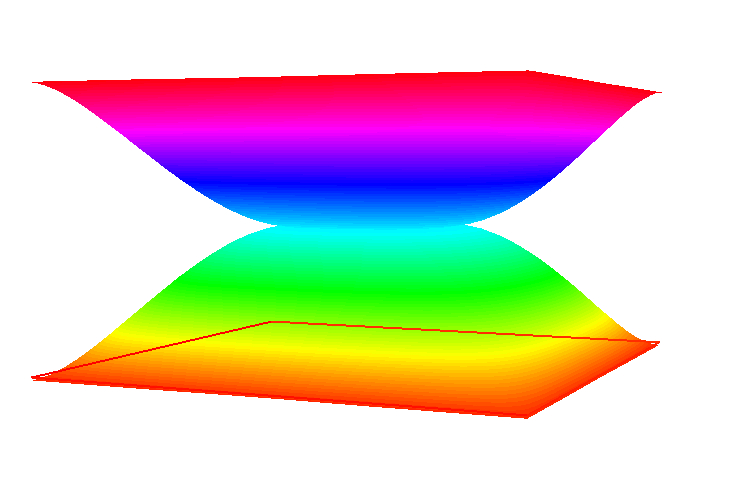
\includegraphics[width=8cm] {VarIneqFill}
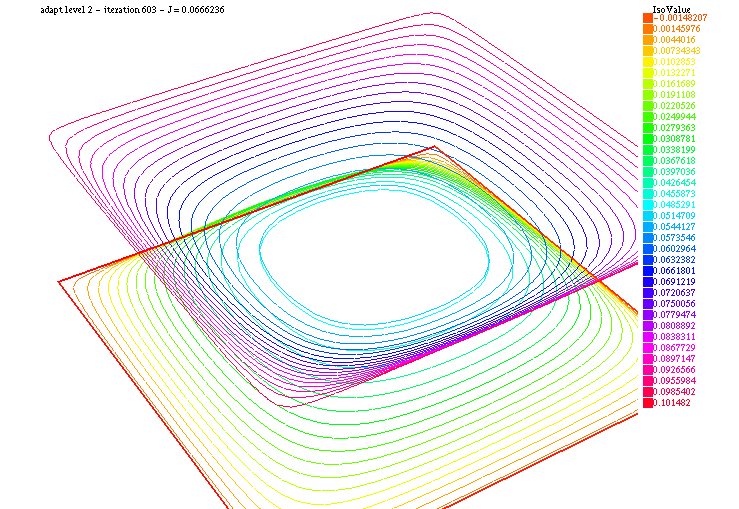
\includegraphics[width=8cm] {VarIneqIso}
\caption{Numerical Approximation of the Variational Inequality \label{VarIneqF}}
\end{figure}

\end{example}

\subsection{3D constrained minimal surface with IPOPT}

\subsubsection{Area and volume expressions}
This example aimed at numerically solving some constrained minimal surface problems with the IPOPT algorithm. We restrain to $C^{k}$ ($k\geq 1$), closed, spherically parametrizable surfaces, i.e. surfaces $S$ such that :
$$ \exists \rho \in C^{k}([0,2\pi ]\times[0,\pi] ) \vert 
S = \left\lbrace 
X = \left(
\begin{array} {c}
 \rhotp \\
 0 \\
 0
\end{array}
\right)
, (\theta,\phi) \in [0,2\pi ]\times[0,\pi]
  \right\rbrace$$
Where the components are expressed in the spherical coordinate system. Let's call $\Omega$ the  $[0,2\pi ]\times[0,\pi]$ angular parameters set. In order to exclude self crossing and opened shapes, the following assumptions upon $\rho$ are made :
$$ \rho \geq 0\ \ \mathrm{and}\ \ \forall \phi, \rho(0,\phi) = \rho(2\pi,\phi)$$
For a given function $\rho$ the first fundamental form (the metric) of the defined surface has the following matrix representation :
\begin{equation}\label{msfff}
G = 
\left(
\begin{array}{c c}
	\rho^{2}\sin^{2}(\phi) + (\dtheta\rho)^{2} &\dtheta\rho\dphi\rho \\
	\dtheta\rho\dphi\rho & \rho^{2} + (\dphi\rho)^{2} \\
\end{array}
\right)
\end{equation}
This metric is used to express the area of the surface. Let $g=\det(G)$, then we have :
\begin{equation}\label{msarea}
	\mathcal{A}(\rho) 
	= \MyInt{\Omega}{\left\| \dtheta X \wedge \dphi X \right\|}
	=\MyInt{\Omega}{\sqrt{g}}
	=\MyInt{\Omega}{\sqrt{ \rho^{2}(\dtheta\rho)^{2}  + \rho^{4}\sin^{2}(\phi) + \rho^{2}(\dphi\rho)^{2}\sin^{2}(\phi)}d\theta d\phi}
\end{equation}
The volume of the space enclosed within the shape is easier to express :
\begin{equation}\label{msvolume}
	\mathcal{V}(\rho)
	= \MyInt{\Omega}{\int_{0}^{\rhotp} r^{2}\sin(\phi) �dr d\theta d\phi}
	= \frac{1}{3}\MyInt{\Omega}{\rho^{3} \sin(\phi) d\theta d\phi}
\end{equation}


\subsubsection{Derivatives}
In order to use a newton based interior point optimization algorithm, one must be able to evaluate the derivatives of $\mathcal{A}$ and $\mathcal{V}$ with respect to $rho$. Concerning the area we have the following result :
$$
	\forall v\in C^{1}(\Omega) \ , \ \langle d\mathcal{A}(\rho),v\rangle
	= \MyInt{\Omega}{\frac{1}{2} \frac{ d\bar{g}(\rho)(v)}{\sqrt{g}}d\theta d\phi   }
$$
Where $\bar{g}$ is the application mapping the $\tp \mapsto g(\theta,\phi)$ scalar field to $\rho$. This leads to the following expression, easy to transpose in a freefem script using :
\begin{equation}\label{msdarea}
	\begin{array}{r c l}
		\forall v\in C^{1}(\Omega) \ , \ \langle d\mathcal{A}(\rho),v\rangle &
		=  & \MyInt{\Omega}{  \left(2\rho^{3}\sin^{2}(\phi) + \rho(\dtheta\rho)^{2} + \rho(\dphi\rho)^{2}\sin^{2}(\phi) \right) v} \\
		& &  +\MyInt{\Omega}{\ \rho^{2}\dtheta\rho\dtheta v\ + \ \rho^{2}\dphi\rho\sin^{2}(\phi)\dphi v   }
	\end{array}
\end{equation}

With a similar approach, one can derive an expression for second order derivatives. Though comporting no specific difficulties, the detailed calculus are tedious, the result is that 
these derivatives can be write using a $3\times 3$ matrix $\bm{B}$ whose coefficients are expressed in term of $\rho$ and its derivatives with respect to $\theta$ and $\phi$, such that :
\begin{equation}\label{msd2area}
	\forall (w,v)\in C^{1}(\Omega)\ ,\  d^{2}\mathcal{A}(\rho)(w,v) = \MyInt{\Omega}
	{
		\left(\begin{array}{c c c} w & \dtheta w &  \dphi w \end{array}\right)
		\bm{B}
	}	\left( \begin{array}{c} v \\ \dtheta v \\ \dphi v \end{array} \right) d\theta d\phi
\end{equation}

Deriving the volume function derivatives is again an easier task. We immediately get the following expressions :
\begin{equation}\label{msdvolume}
	\begin{array}{r c l}
		\forall v\ ,\ \langle d\mathcal{V}(\rho),v\rangle & = & \MyInt{\Omega}{\rho^{2}\sin(\phi)v\ d\theta d\phi} \\
		\forall w,v\ , d^{2}\mathcal{V}(\rho)(w,v) & = & \MyInt{\Omega}{2\rho\sin(\phi)wv\ d\theta d\phi}
	\end{array}
\end{equation}

\subsubsection{The problem and its script :}
The whole code is available in {\tt IpoptMinSurfVol.edp}. We propose to solve the following problem : 

\begin{example} 
Given a positive function $\rho_{\mathrm{object}}$ piecewise continuous, and a scalar $\mathcal{V}_{\mathrm{max}} > \mathcal{V}(\rho_{\mathrm{object}})$,
find $\rho_{0}$ such that :
$$
\rho_{0} = \underset{\rho\in C^{1}(\Omega)}{\operatorname{argmin}}\ \mathcal{A}(\rho)\ ,\ \mathrm{s.t.}\  \rho_{0}\geq\rho_{\mathrm{object}} \ \mathrm{and\ } \mathcal{V}(\rho_{0})\leq \mathcal{V}_{\mathrm{max}}
$$
\end{example}
If $\rho_{\mathrm{object}}$ is the spherical parametrization of the surface of a 3-dimensional object (domain) $\mathcal{O}$, it can be interpreted as finding the surface with minimal area enclosing the object with a given maximal volume.
If $\mathcal{V}_{\mathrm{max}}$ is close to $ \mathcal{V}(\rho_{\mathrm{object}})$, so should be $\rho_{0}$ and $\rho_{\mathrm{object}}$. With higher values of $\mathcal{V}_{\mathrm{max}}$, $\rho$ should 
be closer to the unconstrained minimal surface surrounding $\mathcal{O}$ which is obtained as soon as $\mathcal{V}_{\mathrm{max}} \geq \frac{4}{3}\pi \|\rho_{\mathrm{object}}\|_{\infty}^{3} $ (sufficient but not necessary).
\newline

It also could be interesting to solve the same problem with the constraint $\mathcal{V}(\rho_{0})\geq \mathcal{V}_{\mathrm{min}}$ which lead to a sphere when 
$\mathcal{V}_{\mathrm{min}} \geq \frac{1}{6}\pi \mathrm{diam}(\mathcal{O})^{3} $ and move toward the solution of the unconstrained problem as $\mathcal{V}_{\mathrm{min}}$ decreases.
\newline

We start by meshing the domain $[0,2\pi ]\times\ [0,\pi ]$, then a periodic P1 finite elements space is defined.
\bFF
@load "msh3";
@load "medit";
@load "ff-Ipopt";

@int np=40; //initial mesh quality parameter
@mesh Th = @square(2*np,np,[2*@pi*x,@pi*y]);

@fespace Vh(Th,@P1,@periodic=[[2,y],[4,y]]);
Vh startshape=5; //initial shape
\eFF
We create some finite element functions whose underlying arrays will be used to store the values of dual variables associated to all the constraints in order to reinitialize the algorithm with
it in the case where we use mesh adaptation. Doing so, the algorithm will almost restart at the accuracy level it reached before mesh adaptation, thus saving many iterations.
\bFF
Vh uz=1.,lz=1.; //Simple bounds dual variable
@real@[int] lm=[1]; //dual variable for volume constraint
\eFF
Then, follows the mesh adaptation loop, and a rendering function, {\tt Plot3D},  using 3D mesh to display the shape it is passed with {\tt medit} (the {\tt movemesh23} procedure often crashes
when called with ragged shapes).
\bFF 
@int nadapt=1;
@for(@int kkk=0;kkk<nadapt;++kkk) //Mesh adaptation loop
{

@int iter=0;//iterations count
@func sin2 = @square(@sin(y)); //a function that will be often used

@func @int Plot3D(@real[@int] &rho,@string cmm,@bool ffplot) {...} //see the .edp file
\eFF
Here are the functions related to the area computation and its shape derivative, according to equations \ref{msarea} and \ref{msdarea} :
\bFF
@func @real Area(@real[@int] &X) 
{
  Vh rho;
  rho[] = X;
  Vh rho2 = @square(rho);
  Vh rho4 = @square(rho2);
  @real res = @int2d(Th)(  @sqrt( rho4*sin2 
                              + rho2*@square(@dx(rho)) 
                              + rho2*sin2*@square(@dy(rho)) )  
                       );
  ++iter;
  @plot(rho,  ... /*some parameters*/ ... );
  @return res;
}

@func @real[@int] GradArea(@real[@int] &X) //The gradient
{
  Vh rho,rho2;
  rho[] = X;
  rho2[] = @square(X);
  Vh sqrtPsi,alpha; //Psi is actually det(G)
  {//some optimizations
    Vh  dxrho2 = @dx(rho)*@dx(rho), dyrho2 = @dy(rho)*@dy(rho);
    sqrtPsi = @sqrt( rho2*rho2*sin2 + rho2*dxrho2 + rho2*dyrho2*sin2 );
    alpha = 2.*rho2*rho*sin2 + rho*dxrho2 + rho*dyrho2*sin2;
  }
  @varf dSurface(u,v) = 
    @int2d(Th)(1./sqrtPsi*(alpha*v+rho2*@dx(rho)*@dx(v)+rho2*@dy(rho)*sin2*@dy(v)));
  @real[@int] grad = dSurface(0,Vh);
  @return grad;
}
\eFF
The function returning the hessian of the area for a given shape is a bit blurry, thus we won't show here all of equation \ref{msd2area} coefficients definition, they can be found in the {\tt edp} file. 
\bFF
@matrix hessianA; //The global matrix buffer

@func @matrix HessianArea(@real[@int] &X)
{
  Vh rho,rho2;
  rho[] = X;
  rho2 = @square(rho);
  Vh sqrtPsi,sqrtPsi3,C00,C01,C02,C11,C12,C22,A;
  {
    ... //definition of the above functions
  }
  @varf d2Area(w,v) =
    @int2d(Th)(
      1./sqrtPsi * (A*w*v + 2*rho*@dx(rho)*@dx(w)*v + 2*rho*@dx(rho)*w*@dx(v) 
                    + 2*rho*@dy(rho)*sin2*@dy(w)*v + 2*rho*@dy(rho)*sin2*w*@dy(v)
                    + rho2*@dx(w)*@dx(v) + rho2*sin2*@dy(w)*@dy(v)) 
    + 1./sqrtPsi3 * (C00*w*v + C01*@dx(w)*v + C01*w*@dx(v) + C02*@dy(w)*v 
                    + C02*w*@dy(v) + C11*@dx(w)*@dx(v)
                    + C12*@dx(w)*@dy(v) + C12*@dy(w)*@dx(v) + C22*@dy(w)*@dy(v)) 
     );//end of int2d and varf
  hessianA = d2Area(Vh,Vh);
  @return hessianA;
}
\eFF
And the volume related functions :
\bFF
@func @real Volume(@real[@int] &X)
{
  Vh rho;
  rho[]=X;
  Vh rho3=rho*rho*rho;
  @real res = 1./3.*@int2d(Th)(rho3*@sin(y));
  @return res;
}

@func @real[@int] GradVolume(@real@[int] &X)
{
  Vh rho;
  rho[]=X;
  @varf dVolume(u,v) = @int2d(Th)(rho*rho*@sin(y)*v);
  @real[@int] grad = dVolume(0,Vh);
  @return grad;
}

@matrix hessianV;//buffer
@func @matrix HessianVolume(@real[@int] &X)
{
  Vh rho;
  rho[]=X;
  @varf d2Volume(w,v) = @int2d(Th)(2*rho*@sin(y)*v*w);
  hessianV = d2Volume(Vh,Vh);
  @return hessianV;
}
\eFF
If we want to use the volume as a constraint function
we must wrap it and its derivatives in some FreeFem++ functions returning the appropriate types.
It is not done in the above functions in case where one wants to use it as fitness function.
The lagrangian hessian also have to be wrapped since the Volume is not linear with 
respect to $\rho$, it has some non-null second order derivatives.
\bFF
@func @real[@int] ipVolume(@real[@int] &X) {@real[@int] vol = [Volume(X)]; @return vol;}

@matrix mdV;//buffer
@func @matrix ipGradVolume(@real[@int] &X) 
{//transforms a vector into a sparse matrix
  @real[@int,@int] dvol(1,Vh.ndof);
  dvol(0,:)=GradVolume(X); 
  mdV=dvol; 
  @return mdV;
}

@matrix HLagrangian; //buffer
@func @matrix ipHessianLag(@real[@int] &X,@real objfact,@real[@int] &lambda)
{
  HLagrangian = objfact*HessianArea(X) + lambda[0]*HessianVolume(X);
  @return HLagrangian;
}
\eFF
The {\tt ipGradVolume} function could bring some troubles during the optimization process because the gradient vector is transformed in a sparse matrix, so any null coefficient
will be discarded. We are here obliged to give IPOPT the structure by hand and use the {\tt checkindex} named-parameter to avoid bad indexing during copies. 
This gradient is actually dense, there is no reason for some components to be constantly zero :
\bFF
//sparse structure of a dense vector
@int[@int] gvi(Vh.ndof),gvj=0:Vh.ndof-1;
gvi=0; //only one line
\eFF
These two arrays will be passed to IPOPT with {\tt structjacc=[gvi,gvj]}. The last remaining things are the bounds definition. The simple lower bounds 
must be equal to the components of the P1 projection of $\rho_{object}$. And we choose $\alpha\in [0,1]$ to set $\mathcal{V}_{\mathrm{max}}$ to 
$(1-\alpha) \mathcal{V}(\rho_{object}) + \alpha\frac{4}{3}\pi \|\rho_{\mathrm{object}}\|_{\infty}^{3}$ :
\bFF
@real e=0.1,r0=0.25,rr=2-r0;
@real E=1./(e*e),RR=1./(rr*rr);
//An indented disc
@func disc1 = @sqrt(1./(RR+(E-RR)*@cos(y)*@cos(y)))*(1+0.1*@cos(9*x));
//Almost a standard disc
@func disc2 = @sqrt(1./(RR+(E-RR)*@cos(x)*@cos(x)*sin2))  ;
Vh lb =  @max(disc1, disc2);//glue the object parts
@real Vobj = Volume(lb[]); //object volume
@real Vnvc = 4./3.*@pi*@pow(lb[].linfty,3);//V for no volume constraint
@real alpha=0.1;
Plot3D(lb[],"object_inside",0);
@real[@int] clb=0.,cub=[(1-alpha)*Vobj + alpha*Vnvc];
\eFF
Calling IPOPT :
\bFF
@IPOPT(Area,GradArea,ipHessianLag,
      ipVolume,ipGradVolume,rc[], //functions and starting point
      @ub=ub[],@lb=lb[],@clb=clb,@cub=cub, //simple bounds and volume bounds
      @checkindex=1,@structjacc=[gvi,gvj],//for safe matrices copies
      @maxiter=kkk<nadapt-1 ? 40:150,//accurate optim only for last mesh adaptation iteration
      @warmstart=kkk,@lm=lm,@uz=uz[],@lz=lz[], //warmstart handling
      @tol=0.00001);

Plot3D(rc[],"Shape_at_"+kkk,0); //displays current solution
\eFF
At last, before closing the mesh adaptation loop, we have to perform the said adaptation. The mesh is adaptated with respect to the $X=(\rho,0,0)$ (in spherical coordinates) vector field, not
directly with respect to $\rho$, otherwise the true curvature of the 3D-shape would not be well taken into account.
\bFF
@if(kkk<nadapt-1)
{
  @Th = @adaptmesh(Th,
         rc*@cos(x)*@sin(y),//X
         rc*@sin(x)*@sin(y),//Y
         rc*@cos(y),//Z
         @nbvx=50000,
         @periodic=[[2,y],[4,y]]); //keeps mesh peridicity
  @plot(Th);
  startshape = rc; //shape interpolation on the new mesh
  uz=uz;//dual variables interpolation
  lz=lz;
} //end if
} //en of mesh adaptation loop
\eFF
Here are some pictures of the resulting surfaces obtained for decreasing values of $\alpha$ (and a slightly more complicated object than two orthogonal discs). We get back the enclosed object when $\alpha=0$ :

\begin{center} 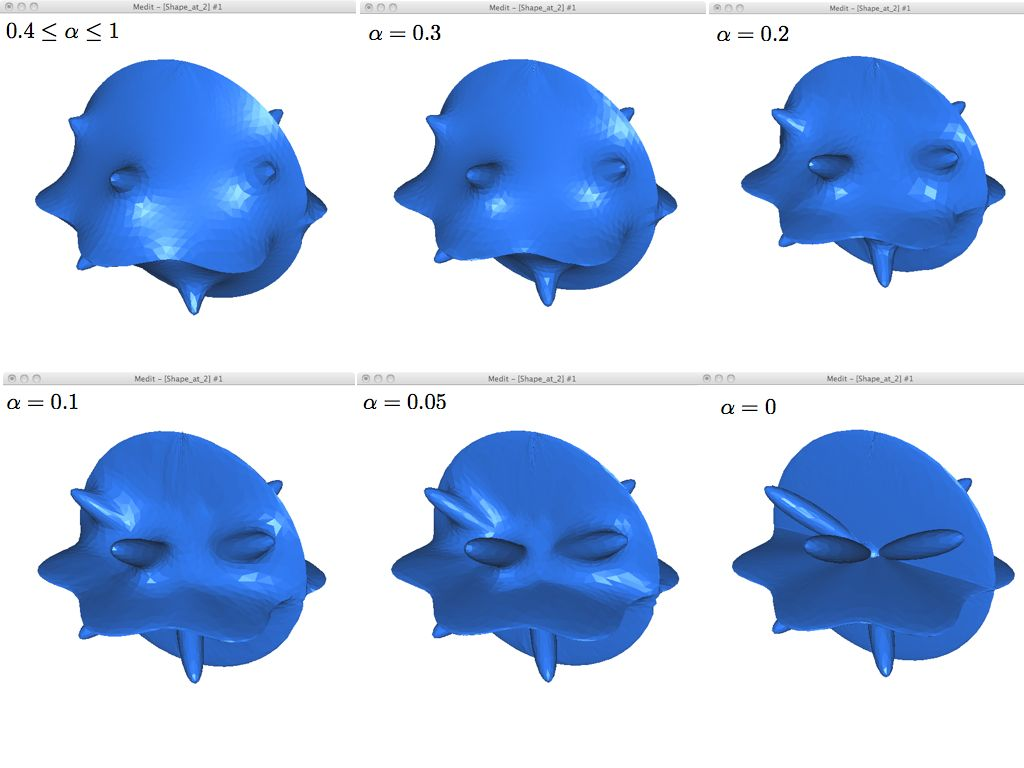
\includegraphics[width=16.5cm] {minsurf3D} \end{center}


\subsection{The nlOpt optimizers}
The {\tt ff-NLopt}  package provides a FreeFem interface to the free/open-source library for nonlinear optimization, thus easing the use of several different free optimization (constrained or not) routines available
online along with the PDE solver. All the algorithms are well documented in \cite{nlopt}, thus no exhaustive informations concerning their mathematical specificities will be found here and we will focus on 
the way they are called in a FreeFem script. One needing detailed informations about these algorithms should visit the said cite where a description of each of them is given, as well as many bibliographical links. 
Most of the gradient based algorithm of nlOpt uses a full matrix approximation of the hessian, so if you're planing to solve a large scale problem, our advise would be to use the IPOPT optimizer which definitely surpass them. Finally, an examples of use can be found in the {\tt examples++-load/} directory under the name {\tt VarIneq2.edp}

All the nlOpt features are called that way :

\bFF
  @load "ff-NLopt"
  ... //define J, u, and maybe grad(J), some constraints etc...
  @real min = nloptXXXXXX(J,u,   //unavoidable part
                         grad = <name of grad(J)> , //if needed
                         lb = //lower bounds array
                         ub= //upper bounds array
                         ...//   some optional arguments :
                            //constraints functions names,
                            //                 stopping criterions,
                            //     algo. specific parameters,
                            //                                           etc...
                         );
\eFF

{\tt XXXXXX} refers to the algorithm tag (not necessarily 6 characters long). {\tt u} is the starting position (a {\tt real[int]} type array) which will be overwritten by the algorithm, the value at the end being the found argmin. And as usual, {\tt J} is a function taking a {\tt real[int]} type array as argument and returning a {\tt real}. {\tt grad}, {\tt lb} and {\tt ub} are "half-optionnal" arguments, in the sense that they are obligatory for some routines but not all.

The possible optional named parameters are the following, note that they are not used by all algorithm s (some does not supports constraints, or a type of constraints, some are gradient-based and other are derivative free, etc...). One can refer to the table after the parameters description to check which are the named parameters supported by a specific algorithm. Using an unsupported parameter will not stop 
the compiler work and seldom breaks runtime, it will just be ignored. That said, when it is obvious you are missusing a routine, you will get a warning message at runtime (for exemple if you pass a gradient 
to a derivative free algorithm, or set the population of a non-genetic one, etc...). In the following description, $n$ stands for the dimension of the search space.\\�\\



\index{ffNLOpt}
\begin{description}

\item[\textbf{Half-optional parameters :}]
\begin{description}
    \item[ ]
    \item[\texttt{grad=}]  The name of the function which computes the gradient of the cost function (prototype should be {\tt real[int]} $\rightarrow$ {\tt real[int]}, both argument and result should have the size $n$). 
    This is needed as soon s a gradient-based method is involved, ignored if defined in a derivative free context. 
    \item[\texttt{lb}/\texttt{ub} =] Lower and upper bounds arrays ({\tt real[int]} type) of size $n$. Used to define the bounds within which the search variable is allowed to move. 
    Needed for some algorithms, optional or unsupported for others.
    \item[\texttt{subOpt} :] Only enabled for the Augmented Lagrangian and MLSL method who need a sub-optimizer in order to work. Just pass the tag of the desired local algorithm with a {\tt string}.
\end{description}

\item[\textbf{Constraints related parameters (optional - unused if not specified):}]
\begin{description}
  \item[ ]
  \item[\texttt{IConst}/\texttt{EConst} :] Allows to pass the name of a function implementing some inequality (resp. equality) constraints on the search space. The function type must be 
  {\tt real[int]} $\rightarrow$ {\tt real[int]} where the size of the returned array is equal to the number of constraints (of the same type - it means that all the constraints are computed in one vectorial function).
  In order to mix inequality and equality constraints in a same minimization attempt, two vectorial functions have to be defined and passed. See example \ref{varineqex} for more details about how these
  constraints have to be implemented.
  \item[\texttt{gradIConst}/\texttt{gradEConst} :] Use to provide the inequality (resp. equality) constraints gradient. These are {\tt real[int]} $\rightarrow$ {\tt real[int,int]} type functions. Assuming we have defined
  a constraint function (either inequality or equality) with $p$ constraints, the size of the matrix returned by its associated gradient must be $p\times n$ (the $i$-th line of the matrix is the gradient of the $i$-th
  constraint). It is needed in a gradient-based context as soon as an inequality or equality constraint function is passed to the optimizer and ignored in all other cases.
  \item[\texttt{tolIConst}/\texttt{tolEConst} :] Tolerance values for each constraint. This is an array of size equal to the number of inequality (resp. equality) constraints. Default value os set to $10^{-12}$
  for each constraint of any type.  
\end{description}

\item[\textbf{Stopping criteria :}]
\begin{description}
  \item[ ]
  \item[\texttt{stopFuncValue} :] Makes the algorithm end when the objective function reaches this {\tt real} value.
  \item[\texttt{stopRelXTol} :] Stops the algorithm when the relative moves in each direction of the search space is smaller than this {\tt real} value.
  \item[\texttt{stopAbsXTol} :] Stops the algorithm when the moves in each direction of the search space is smaller than the corresponding value in this {\tt real[int]} array.
  \item[\texttt{stopRelFTol} :] Stops the algorithm when the relative variation of the objective function is smaller than this {\tt real} value.
  \item[\texttt{stopAbsFTol} :] Stops the algorithm when the variation of the objective function is smaller than this {\tt real} value.
  \item[\texttt{stopMaxFEval} :] Stops the algorithm when the number of fitness evaluations reaches this {\tt integer} value.
  \item[\texttt{stopTime} :] Stops the algorithm when the otpimization time in second exceeds this {\tt real} value. This is not a strict maximum: the time may exceed it slightly, 
  depending upon the algorithm and on how slow your function evaluation is.
 \end{description}
 Note that when an AUGLAG or MLSL method is used, the meta-algorithm and the sub-algorithm may have different termination criteria. Thus, for algorithms of this kind, the following
 named parameters has been defined (just adding the SO prefix - for Sub-Optimizer) to set the ending condition of the sub-algorithm (the meta one uses the ones above) : {\tt SOStopFuncValue}, 
 {\tt SOStopRelXTol}, and so on... If these ones are not used, the sub-optimizer will use those of the master routine.
 
 \item[\textbf{Other named parameters :}]
 \begin{description}
   \item[ ]
   \item[\texttt{popSize} :] {\tt integer} used to change the size of the sample for stochastic search methods. Default value is a peculiar heuristic to the chosen algorithm.
   \item[\texttt{SOPopSize} :] Same as above, but when the stochastic search is passed to a meta-algorithm.
   \item[\texttt{nGradStored} :] The number ({\tt interger} type) of gradients to "remember" from previous optimization steps: increasing this increases the memory requirements but may speed convergence.
   It is set to a heuristic value by default. If used with AUGLAG or MLSL, it will only affect the given subsidiary algorithm.
 \end{description}

\end{description}

The following table sums up the main characteristics of each algorithm, providing the more important information about which features are supported by which algorithm and what are the unavoidable arguments 
they need. More details can be found in \cite{nlopt}.
\begin{center}
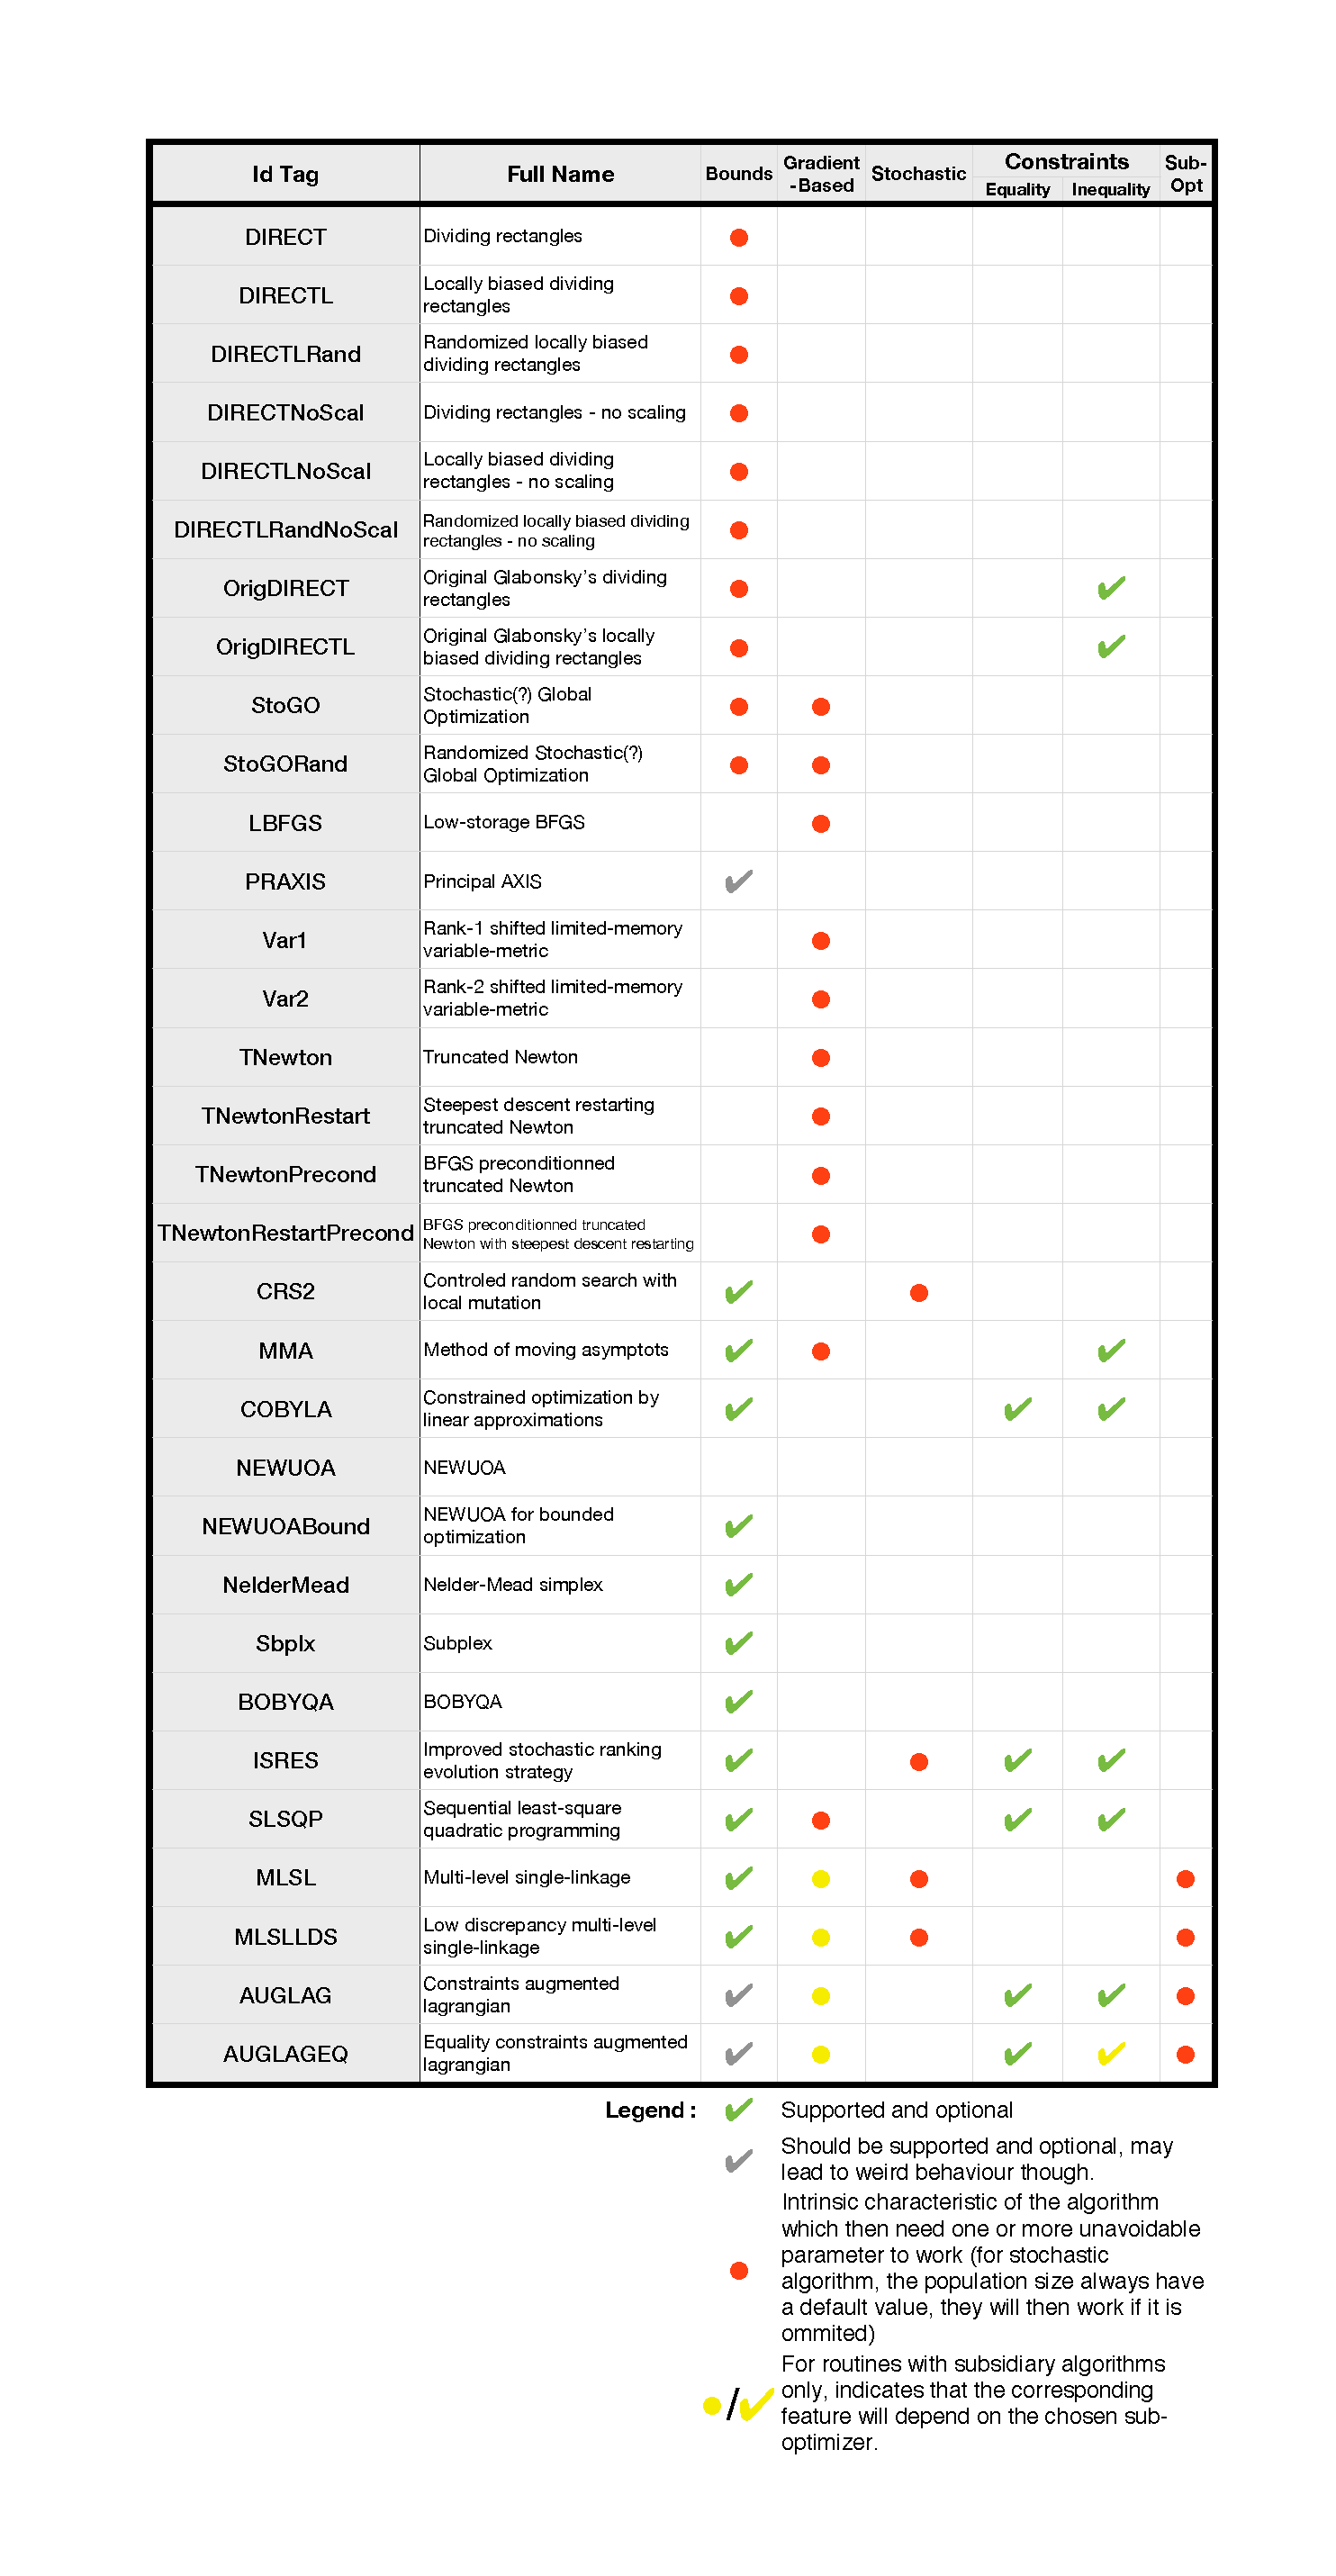
\includegraphics [height=\textheight]{nlopttab}   
\end{center}


%\begin{example}[VarIneq.edp]
%\label{varineqex}
%Let $\Omega$ be a domain of $\mathbb{R}^{2}$, $f_{1}, f_{2}\in L^{2}(\Omega)$ and $g_{1}, g_{2} \in L^{2}(\partial\Omega)$ four given functions with $g_{1}\leq g_{2}$ almost everywhere.
%We define the space : 
%$$V = \left\lbrace (v_{1},v_{2})\in H^{1}(\Omega)^{2} ; v_{1}\vert_{\partial\Omega}=g_{1}, v_{2}\vert_{\partial\Omega}=g_{2}, v_{1}\leq v_{2}\ \mathrm{a.e.}\ \right\rbrace$$
%as well as the functional $J:H^{1}(\Omega)^{2}\longrightarrow \mathbb{R}$:
%$$J(v_{1},v_{2}) = \displaystyle{\frac{1}{2}\int_{\Omega}\vert\nabla v_{1}\vert^{2} - \int_{\Omega} f_{1}v_{1} +  \frac{1}{2}\int_{\Omega}\vert\nabla v_{2}\vert^{2} - \int_{\Omega} f_{2}v_{2}}$$
%The problem consists in finding (numerically) two functions $(u_{1},u_{2}) = \underset{(v_{1},v_{2})\in V}{\operatorname{argmin}} J(v_{1},v_{2}) $.
%
%This can be interpreted as finding $u_{1}, u_{2}$ as close as possible (in a certain sense) to the solutions of Laplace equation with respectively $f_{1}, f_{2}$ second members
% and $g_{1}, g_{2}$ Dirichlet boundary conditions with the $u_{1}\leq u_{2}$ almost everywhere constraint.
%\end{example}
%
%Here is the corresponding script to treat this variational inequality problem with one of the NLOpt algorithms. The whole script is in the \texttt{VarIneq2.edp}.
%\bFF
%  @load "ff-NLopt" //Loading nlopt
%  @int NN = 10;
%  @mesh Th = @square(NN,NN);
%  @func f1=1.; //Datas
%  @func f2=-1.; 
%  @func g1=0.;
%  @func g2=0.1;
%  @int nadapt=3,iter=0;
%  @real starttol=1e-12,bctol=6.e-12;
%  @fespace Vh(Th,P1);
%\eFF
%
%Instead of defining the $J$ functional with explicit integral on the domain, we will write it in quadratic/linear form, since the corresponding matrix and vector will not change
%along with the iterations and the FreeFem matrix-vector product is optimized, this method will significantly speed up the approximation of the solution.
%
%\bFF
%  @varf BVF(v,w) = @int2d(Th)(0.5*@dx(v)*@dx(w) + 0.5*@dy(v)*@dy(w)); //bilinear
%  @varf LVF1(v,w) = @int2d(Th)(f1*w);//and linear parts
%  @varf LVF2(v,w) = @int2d(Th)(f2*w);
%  @matrix A =  BVF(Vh,Vh);//corresponding matrix
%  @real[@int] b1 = LVF1(0,Vh) , b2 = LVF2(0,Vh); //and vectors
%\eFF
%Then follows a trick that we will use later to pass the boundary conditions as non-linear equality constraints (although these are of course linear ones, but this approach
%demonstrate how to use all the features of NLOpt in one shot).
%\bFF
%  @varf Vbord(v,w) = @on(1,2,3,4,v=1);
%  Vh In,Bord;
%  Bord[] = Vbord(0,Vh,@tgv=1); //Bord=1 on the border
%  In[] = Bord[] ? 0:1; //and 0 inside
%  Vh gh1=Bord*g1,gh2=Bord*g2; //gh1=g1 on the border and 0 inside
%  
%  //The functional :
%  @func @real J(@real[@int] &X)
%  {
%    Vh u1,u2;
%    u1[] = X(0:Vh.ndof-1); //splitting the vector
%    u2[] = X(Vh.ndof:2*Vh.ndof-1); 
%    iter++;
%	    @real[@int] Au1 = A*u1[], Au2 = A*u2[]; 
%	    Au1 -= b1;
%	    Au2 -= b2;
%	    @real val = u1[]'*Au1 + u2[]'*Au2;
%	    @plot(u1,u2,...); //parameters omitted
%	    @return val;
%  }
%\eFF
%To be able to play with gradient-based algorithm, we must have a gradient ready :
%\bFF
%  @varf dBFV(v,w) = @int2d(Th)(@dx(v)*@dx(w)+@dy(v)*@dy(w)); 
%  @matrix dA = dBFV(Vh,Vh);
%  @func @real[@int] dJ(@real[@int] &X)
%  {
%	    Vh u1,u2;
%	    u1[] = X(0:Vh.ndof-1);
%	    u2[] = X(Vh.ndof:2*Vh.ndof-1);
%	    @real[@int] grad1 = dA*u1[], grad2 = dA*u2[];
%	    grad1 -= b1;
%	    grad2 -= b2;
%	    @real[@int] Grad(X.n);
%	    Grad(0:Vh.ndof-1) = grad1;
%	    Grad(Vh.ndof:2*Vh.ndof-1) = grad2; 
%	    @return Grad;
%  }
%\eFF
%As we use P1 Lagrange finite elements, the $u_{1}\leq u_{2} $ constraint can be expressed directly upon the degree of freedom. In NLOpt, one constraint must have the form $f(X)\leq 0$.
%The function is vectorial in order to handle multiple constraints :
%\bFF
%  @func @real[@int] IneqC(@real[@int] &X)
%  {
%	    @real[@int] constraints(Vh.ndof);
%	    @for(@int i=0;i<Vh.ndof;++i) constraints[i] = X[i] - X[i+Vh.ndof];
%	    @return constraints; //u1i - u2i <= 0
%  }
%\eFF
%One also has to define a gradient for each constraint if a gradient search is to be used. Constraint gradient must be a function which returns a matrix. The $i$-th line of this matrix is the gradient of
%the $i$-th constraint with respect to the variables of the search space.
%\bFF
%  @func @real[@int,@int] dIneqC(@real[@int] &X)
%  {
%	    @real[@int,@int] dconst(Vh.ndof,2*Vh.ndof);//so sparse... shame!
%	    dconst=0;
%	    @for(@int i=0;i<Vh.ndof;++i)
%	    {
%		      dconst(i,i) = 1.;
%		      dconst(i,i+Vh.ndof) = -1.;
%	    }
%	    @return dconst;
%  }
%\eFF
%As mentioned earlier, we also define a set of equality constraints and their derivatives in order to handle the boundary conditions. One could also use the {\tt lb} and {\tt ub} parameters to impose them, this also would avoid the use of large sparse matrix returned by the gradient function (it can be found in the script file, where we set {\tt lb} to $g-\epsilon$ and {\tt ub} to $g+\epsilon$).
%Here again, we can work directly on the degree of freedom because of the P1 finite element. The script could not work with other finite elements without modifications.
%\bFF
%  @real[@int] BordIndex(Th.nbe); //Indexes of border d.f.
%  
%  {
%	    @int k=0; //filling the index array
%	    @for(@int i=0;i<Bord.n;++i) if(Bord[][i]) {BordIndex[k]=i; ++k;}
%  }
%  
%  @func @real[@int] BC(@real[@int] &X)
%  {
%	    @real[@int] bc(2*Th.nbe);
%	    @for(@int i=0;i<Th.nbe;++i)
%	    {
%		      @int I = BordIndex[i];
%		      bc[i] = X[I] - gh1[][I];
%		      bc[i+Th.nbe] = X[I+Th.nv] - gh2[][I];
%	    }
%	    @return bc;
%  }
%  @func @real[@int,@int] dBC(@real[@int] &X) //Gradient of boundary conditions
%  {
%	    @real[@int,@int] dbc(2*Th.nbe,2*Th.nv);//even sparser...:(
%	    dbc=0.;
%	    @for(@int i=0;i<Th.nbe;++i)
%	    {
%		      @int I=BordIndex[i];
%		      dbc(i,I) = 1.;
%		      dbc(i+Th.nbe,I+Th.nv) = 1.;
%	    }
%	    @return dbc;
%  }
%\eFF
%Now we fill an initial vector and start the algorithm :
%\bFF
%  @real[@int] start(2*Vh.ndof);
%  start(0:Vh.ndof-1) = 0.; //starting with u1=u2=0 is bad
%  start(Vh.ndof:2*Vh.ndof-1) = 0.01; //a small difference is needed
%  
%  @real mini = @nloptAUGLAG(J, start, @grad=dJ,
%                          @IConst=IneqC, @gradIConst=dIneqC,
%                          @EConst=BC, @gradEConst=dBC,
%                          @subOpt="LBFGS", 
%                          @stopMaxFEval=10000, @stopAbsFTol=starttol
%                         );
%\eFF
%Here we wrap a BFGS algorithm (which only works with unconstraint problems) in the augmented lagrangian method for both equality and inequality constraints. Another legit choice would be to use
%SLSQP, the only gradient-based search of the package supporting these two kinds of constraints (note that the {\tt subOpt} parameter is gone ) :
%\bFF
%  @real mini = @nloptSLSQP(J, start, @grad=dJ,
%                          @IConst=IneqC, @gradIConst=dIneqC,
%                          @EConst=BC, @gradEConst=dBC,
%                          @stopMaxFEval=10000, @stopAbsFTol=starttol
%                         );
%\eFF
%One can also try to pass derivative free algorithms to AUGLAG and discard the gradients to see what happens, or directly one which handles the two kinds of constraints. Just check 
%the tag in the table. The true script also has a loop in which the algorithm is restarted after mesh adaptation, nothing was said about that to avoid complicating an already relatively long
%script comment.








\subsection{Optimization with MPI}
The only quick way to use the previously presented algorithms on a parallel architecture lies in parallelizing the used cost function (which is in most real life case, the expensive part of the algorithm).
 Somehow, we provide a parallel version of the CMA-ES algorithm. The parallelization principle is the trivial one of evolving/genetic algorithms : at each iteration the cost function has to be evaluated $N$ 
 times without any dependence at all, these $N$ calculus are then equally distributed to each processes. Calling the MPI version of CMA-ES is nearly the same as calling its sequential version (a 
 complete example of use can be found in the \texttt{cmaes-mpi-VarIneq.edp} file).:

\bFF
  @load "mpi-cmaes"
  ... //define J, u and all here
  @real min = cmaesMPI(J,u,stopTolFun=1e-6,stopMaxIter=3000);
  @cout << "minimal value is " << min << " for u = " << u << @endl;
\eFF

If the population size is not changed using the {\tt popsize} parameter, it will use the heuristic value slightly changed to be equal to the closest greater multiple of the size of the communicator used by 
the optimizer. 
The FreeFem {\tt mpicommworld} is used by default. The user can specify his own MPI communicator with the named parameter "{ \tt comm=}", see the MPI section of this manual for more informations about 
communicators in \texttt{FreeFem++}.



%%%%%%%%%  old -----
%%% \subsection{conjugate Gradient/GMRES}
%%%
%%%Suppose we want to solve  the Euler problem (here $x$ has nothing to do with the reserved variable for the first coordinate in \freefempp): find $ x\in \R^n $  such that
%%%\begin{equation}
%%%\label{eqn:dJ=0}
%%%\nabla J(x) = \left(\frac{\p J}{\p x_i} (\vec{x})\right) = 0
%%%\end{equation}
%%%where $ J$ is a functional (to minimize  for example) from  $ \R^n$ to $ \R$.
%%%
%%%If the function is convex we can use the conjugate gradient to solve the problem,
%%%and we just need the function (named \texttt{dJ} for example)
%%%which compute $\nabla J$, so the parameters
%%%are the name of that function with prototype
%%%
%%% \ttCC{@func\ @real[@int]\  dJ(@real[@int] \& xx);}
%%% 
%%% which compute $\nabla J$, and
%%%a vector \ttCC{x} of type ( of course the number 20 can be changed)
%%%
%%% \ttCC{@real[@int] x(20);} 
%%% 
%%% to initialize the process and get the result.
%%%\\\\
%%%Given an initial value $\vec{x}^{(0)}$, a maximum number $i_{\max}$
%%%of iterations, and an error tolerance $0<\epsilon<1$:
%%%Put $\vec{x}=\vec{x}^{(0)}$ and write
%%%\begin{quote}\texttt{
%%%NLCG($\nabla J$, $\vec{x}$, precon$=M$, nbiter$=i_{\max}$, eps$=\epsilon$);
%%%}
%%%\end{quote}
%%%will give the solution of $\vec{x}$ of $\nabla J(\vec{x})=0$.
%%%We can omit parameters \texttt{precon, nbiter, eps}.
%%%Here $M$ is the preconditioner whose default is the identity matrix.
%%%The stopping test is
%%%\[
%%%\| \nabla J(\vec{x})\|_P\le \epsilon\| \nabla J(\vec{x}^{(0)})\|_P
%%%\]
%%%Writing the minus value in \texttt{eps=}, i.e.,
%%%\begin{quote}\texttt{
%%%NLCG($\nabla J$, $\vec{x}$, precon$=M$, nbiter$=i_{\max}$, eps$=-\epsilon$);
%%%}
%%%\end{quote}
%%%we can use the stopping test
%%%\[
%%%\| \nabla J(\vec{x})\|_P^2\le \epsilon
%%%\]
%%%The  parameters of these three functions are:
%%%% FFCS(8/10/9)need to move index for htindex not to interfere
%%%% with \begin{description}
%%%\index{LinearCG}
%%%\index{LinearCG!nbiter=} \index{LinearCG!precon=} \index{LinearCG!eps=}\index{LinearCG!veps=}
%%%\index{NLCG!nbiter=}  \index{NLCG!eps=}\index{NLCG!veps=}
%%%\index{LinearGMRES}
%%%\index{LinearGMRES!nbiter=} \index{LinearGMRES!precon=} \index{LinearGMRES!eps=}\index{LinearGMRES!veps=}
%%%\begin{description}
%%%
%%%\itemtt[nbiter=] set the number of iteration (by default $100$)
%%%\itemtt[precon=] set the preconditioner function (\texttt{P} for example)   by default it is the identity, remark the prototype
%%%is \ttCC{@func\ @real[\@int]\ P(@real[@int] \&x)}.
%%%\itemtt[eps=] set the value of the stop test $\varepsilon$ ($=10^{-6}$ by default) if positive then relative test
%%%$||\nabla J(x)||_P\leq \varepsilon||\nabla J(x_0)||_P$, otherwise the  absolute test is  $||\nabla J(x)||_P^2\leq |\varepsilon|$.
%%%\itemtt[veps=] set and return the value of the stop test,  if positive then relative test
%%%$||\nabla J(x)||_P\leq \varepsilon||\nabla J(x_0)||_P$, otherwise the  absolute test is  $||\nabla J(x)||_P^2\leq |\varepsilon|$.
%%%The return value is  minus  the real stop test (remark: it is useful in loop).
%%%
%%%\end{description}
%%%
%%%\begin{example}[algo.edp]
%%%For a given function $b$, let us find the minimizer $u$ of the functional
%%%\begin{eqnarray*}
%%% J(u) &=& \frac{1}{2}\int_{\Omega} f(|\nabla u|^2) - \int_{\Omega}  u b \\
%%% f(x) &=& ax + x-\ln(1+x), \quad f'(x) = a+\frac{x}{1+x}, \quad f''(x) =  \frac{1}{(1+x)^2}
%%%\end{eqnarray*}
%%%under the boundary condition $u=0$ on $\p\Omega$.
%%%\bFF
%%%@func @real J(real[int] & u)
%%%  {
%%%    Vh w;w[]=u; // copy array u in the finite element function w
%%%    @real r=@int2d(Th)(0.5*f( dx(w)*dx(w) + dy(w)*dy(w) ) - b*w) ;
%%%    cout << "J(u) =" << r << " " << u.min <<  " " << u.max << endl;
%%%    @return r;
%%%  }
%%%// -----------------------
%%%
%%%Vh u=0; //  the current value of the solution
%%%Ph alpha; // of store  $df(|\nabla u|^2)$
%%%@int iter=0;
%%%alpha=df( dx(u)*dx(u) + dy(u)*dy(u) ); // optimization
%%%
%%%@func @real[int] dJ(@real[@int] & u)
%%%  {
%%%    @int verb=verbosity; verbosity=0;
%%%    Vh w;w[]=u;  // copy array u in the finite element function w
%%%    alpha=df( dx(w)*dx(w) + dy(w)*dy(w) ); // optimization
%%%    @varf au(uh,vh) = @int2d(Th)( alpha*( dx(w)*dx(vh) + dy(w)*dy(vh) ) - b*vh)
%%%                      + @on(1,2,3,4,uh=0);
%%%    u= au(0,Vh);
%%%    verbosity=verb;
%%%    @return u; // warning no return of local array
%%%  }
%%%
%%%\eFF
%%%
%%%We want to construct also a preconditioner $C$
%%%with solving the problem:  find $u_h \in V_{0h}$ such that
%%%\[
%%%\forall v_h \in V_{0h}, \quad  \int_\Omega \alpha \nabla u_h . \nabla v_h = \int_\Omega b v_h
%%%\]
%%%where $ \alpha=f'(|\nabla u|^2)$.
%%%*/
%%%\bFF
%%%@varf alap(uh,vh)=  @int2d(Th)( alpha *( dx(uh)*dx(vh) + dy(uh)*dy(vh) ))
%%%                   + @on(1,2,3,4,uh=0);
%%%
%%%@varf amass(uh)= @int2d(Th)( uh*vh)  + @on(1,2,3,4,uh=0);
%%%
%%%@matrix Amass = alap(Vh,Vh,solver=CG); // \index{matrix}
%%%@matrix Alap=  alap(Vh,Vh,solver=Cholesky,factorize=1);   // \index{Cholesky}\index{factorize=}\index{solver=}
%%%
%%%// the preconditionner function
%%%@func @real[@int] C(@real[@int] & u)
%%%{
%%%   @real[@int] w = Amass*u;
%%%   u = Alap^-1*w;
%%%   @return u; // no return of local array  variable
%%%}
%%%\eFF
%%%/*
%%%To solve the problem, we make 10 iteration of the conjugate gradient,
%%%recompute the preconditioner and restart the conjugate gradient:
%%%*/
%%%\bFF
%%%   verbosity=5;
%%%   @int conv=0;
%%%   @real eps=1e-6;
%%%   @for(@int i=0;i<20;i++)
%%%   {
%%%     conv=NLCG(dJ,u[],nbiter=10,precon=C,veps=eps); // \index{veps=}\index{NLCG}
%%%     @if (conv) @break;  // if converge break loop
%%%     alpha=df( dx(u)*dx(u) + dy(u)*dy(u) ); // recompute alpha optimization
%%%     Alap = alap(Vh,Vh,solver=Cholesky,factorize=1);
%%%     @cout << " restart with new preconditionner " << conv
%%%           << " eps =" << eps << endl;
%%%    }
%%%
%%%   @plot (u,wait=1,cmm="solution with NLCG");
%%%\eFF
%%%\end{example}
%%%For a given symmetric positive matrix $A$, consider the quadratic form
%%%\[
%%%J(\vec{x})=\frac{1}{2}\vec{x}^TA\vec{x}-\vec{b}^T\vec{x}
%%%\]
%%%then $J(\vec{x})$ is minimized by the solution $\vec{x}$ of $A\vec{x}=\vec{b}$.
%%%In this case, we can use the function \texttt{LinearCG}
%%%\begin{quote}\texttt{
%%%LinearCG($A$, $\vec{x}$, precon$=M$, nbiter$=i_{\max}$, eps$=\pm\epsilon$);
%%%}
%%%\end{quote}
%%%If $A$ is not symmetric, we can use GMRES(Generalized Minimum Residual) algorithm by
%%%\begin{quote}\texttt{
%%%LinearGMRES($A$, $\vec{x}$, precon$=M$, nbiter$=i_{\max}$, eps$=\pm\epsilon$);
%%%}
%%%\end{quote}
%%%Also, we can use the non-linear version of GMRES algorithm
%%%(the functional $J$ is just convex)
%%%\begin{quote}\texttt{
%%%LinearGMRES($\nabla J$, $\vec{x}$, precon$=M$, nbiter$=i_{\max}$, eps$=\pm\epsilon$);
%%%}
%%%\end{quote}
%%%For detail of these algorithms, refer to \cite{Lucquin}[Chapter IV, 1.3].
%%%
%%%\subsection{Optimization}
%%%%Two algorithms of
%%%%COOOL  a package \cite{coool} are interfaced with
%%%%the Newton Raphson method  (call \texttt{Newton}) and
%%%%the  \texttt{BFGS} method. \index{Newton}\index{BFGS}
%%%%Be careful of these algorithms, because their
%%%%implementation use full matrices.
%%%%
%%%%Example of utilization
%%%%%\begin{example}[{algo.edp}
%%%%\bFF
%%%%  real[int] b(10),u(10);
%%%%  func @real J(@real[int] & u)
%%%%    {
%%%%      @real s=0;
%%%%      @for (@int i=0;i<u.n;i++)
%%%%          s +=(i+1)*u[i]*u[i]*0.5 - b[i]*u[i];
%%%%      @cout << "J ="<< s << " u =" <<  u[0] << " " << u[1] << "...\n" ;
%%%%      @return s;
%%%%    }
%%%%
%%%%//  the grad of J (this is a affine version (the RHS is in  )
%%%%  @func @real[int] DJ(@real[int] &u)
%%%%    {
%%%%      @for (@int i=0;i<u.n;i++)
%%%%        u[i]=(i+1)*u[i]-b[i];
%%%%      @return u;  // return of global variable ok
%%%%    };
%%%%
%%%%  b=1; u=2; // set  right hand side and initial gest
%%%%  @BFGS(J,dJ,u,eps=1.e-6,nbiter=20,nbiterline=20);
%%%%  @cout << "BFGS: J(u) = " << J(u) << endl;
%%%%
%%%%\eFF
%%%%%\end{example}
%%%Two algorithms of
%%%COOOL  a package \cite{coool} are interfaced with
%%%the Newton Raphson method  (call \texttt{Newton}) and
%%%the  \texttt{BFGS} method. \index{Newton}\index{BFGS}
%%%These two ones are directly available in FreeFem (no dynamical link to load).
%%%Be careful with these algorithms, because their
%%%implementation uses full matrices. We also provide several
%%%optimization algorithms from the NLopt library  \cite{nlopt} as well 
%%%as an interface for Hansen's  implementation of CMAES 
%%%(a MPI version of this one is also available). These last algorithms can
%%%be found as dynamical links in the \texttt{example++-load} folder
%%%as the \texttt{ff-NLopt} and \texttt{CMA\_ES} files (\texttt{CMA\_ES\_MPI}
%%%from the \texttt{example++-mpi} folder for the mpi version).
%%%
%%%\subsubsection{Example of utilization for BFGS or CMAES}
%%%%\begin{example}[{algo.edp}
%%%\bFF
%%%  @real[int] b(10),u(10);
%%%  @func @real J(@real[int] & u)
%%%    {
%%%      @real s=0;
%%%      @for (@int i=0;i<u.n;i++)
%%%          s +=(i+1)*u[i]*u[i]*0.5 - b[i]*u[i];
%%%      @cout << "J ="<< s << " u =" <<  u[0] << " " << u[1] << "...\n" ;
%%%      @return s;
%%%    }
%%%
%%%//  the grad of J (this is a affine version (the RHS is in  )
%%%  @func @real[int] DJ(@real[int] &u)
%%%    {
%%%      @for (@int i=0;i<u.n;i++)
%%%        u[i]=(i+1)*u[i]-b[i];
%%%      @return u;  // return of global variable ok
%%%    };
%%%
%%%  b=1; u=2; // set  right hand side and initial gest
%%%  @BFGS(J,dJ,u,eps=1.e-6,nbiter=20,nbiterline=20);
%%%  @cout << "BFGS: J(u) = " << J(u) << endl;
%%%
%%%\eFF
%%%%\end{example}
%%%
%%%Using the CMA evolution strategy is almost the same, except that, as it is
%%%a derivative free optimizer, the \texttt{dJ} argument is omitted and there are
%%%some other named parameters to control the behaviour of the algorithm. With the same 
%%%objective function as above, an example of utilization would be (see \texttt{cmaes-VarIneq.edp} for a complete example):
%%%\bFF
%%%  @load "ff-cmaes"
%%%  ... //define J, u and all here
%%%  @real min = cmaes(J,u,stopTolFun=1e-6,stopMaxIter=3000);
%%%  @cout << "minimal value is " << min << " for u = " << u << @endl;
%%%\eFF
%%%This algorithm works with a normal multivariate distribution in the parameters
%%%space and try to adapt its covariance matrix using the information provides by
%%%the successive function evaluations (see \cite{hansen} for more details). Thus, some specific parameters can be passed
%%%to control the starting distribution, size of the sample generations etc... Named parameters
%%%for this are the following :
%%%\index{CMAES}
%%%\begin{description}
%%%
%%%    \item[\texttt{seed=}] Seed for random number generator  \index{CMAES!seed=}
%%%    ({\tt val} is an integer). No specified value will lead to a clock based seed initialization.
%%%    
%%%    \item[\texttt{initialStdDev=}] Value for the standard deviations of the initial covariance matrix \index{CMAES!initialStdDev=}
%%%    ({\tt val} is a real). If the value $\sigma$ is passed, the initial covariance matrix will be set to $\sigma I$. The 
%%%            expected initial distance between initial $X$ and the $argmin$
%%%            should be roughly initialStdDev. Default is $0.3$.
%%%    
%%%    \item[\texttt{initialStdDevs=}] Same as above except that the argument is an array allowing to set a value of the initial standard deviation
%%%    for each parameter. Entries differing by several orders of magnitude should be avoided (if it can't be, try rescaling the problem).
%%%    
%%%    \item[\texttt{stopTolFun=}]  Stops the algorithm if function values differences are smaller than the passed one, default is $10^{-12}$.
%%%    
%%%    \item[\texttt{stopTolFunHist=}]  Stops the algorithm if function value differences of the best values are smaller than the passed one, default is $0$ (unused).
%%%    
%%%    \item[\texttt{stopTolX=}]  Stopping criteria triggered if step sizes in the parameters space are 
%%%                 smaller than this real value, default is $0$.
%%%                 
%%%    \item[\texttt{stopTolXFactor=}]  Stopping criteria triggered when the standard deviation increases more than this value. The default value is $10^{3}$.
%%%       
%%%    \item[\texttt{stopMaxFunEval=}]  Stops the algorithm when {\tt stopMaxFunEval} function evaluations have been done. Set to $900(n+3)^{2}$ by default, where $n$ is the parameters space dimension .
%%%                 
%%%    \item[\texttt{stopMaxIter=}]  Integer stopping the search when {\tt stopMaxIter} generations has been sampled. Unused by default.
%%%    
%%%    \item[\texttt{popsize=}]  Integer value used to change the sample size. The default value is $4+ \lfloor 3\ln (n) \rfloor$, see \cite{hansen}
%%%    for more details. Increasing the population size usually improves the global search capabilities at the cost of an at most linear reduction of the convergence speed with respect to {\tt popsize}.
%%%    
%%%    \item[\texttt{paramFile=}] This {\tt string} type parameter allows the user to pass all the parameters using an extern file as in Hansen's original code. More parameters related to the CMA-ES algorithm 
%%%    can be changed with this file. A sample of it can be found in the {\tt examples++-load/ffCMAES/} folder under the name {\tt initials.par}. Note that the parameters passed to the CMAES function in the 
%%%    FreeFem script will be ignored if an input parameters file is given.
%%%                 
%%%\end{description}
%%%
%%%
%%%\subsubsection{The nlOpt optimizers}
%%%The {\tt ff-NLopt}  package provides a FreeFem interface to the free/open-source library for nonlinear optimization, thus easing the use of several different free optimization (constrained or not) routines available
%%%online along with the PDE solver. All the algorithms are well documented in \cite{nlopt}, thus no exhaustive informations concerning their mathematical specificities will be found here and we will focus on 
%%%the way they are called in a FreeFem script. One needing detailed informations about these algorithms should visit the said cite where a description of each of them is given, as well as many bibliographical links.
%%%
%%%All the nlOpt features are called that way :
%%%
%%%\bFF
%%%  @load "ff-NLopt"
%%%  ... //define J, u, and maybe grad(J), some constraints etc...
%%%  @real min = nloptXXXXXX(J,u,   //unavoidable part
%%%                         grad = <name of grad(J)> , //if needed
%%%                         lb = //lower bounds array
%%%                         ub= //upper bounds array
%%%                         ...//   some optional arguments :
%%%                            //constraints functions names,
%%%                            //                 stopping criterions,
%%%                            //     algo. specific parameters,
%%%                            //                                           etc...
%%%                         );
%%%\eFF
%%%
%%%{\tt XXXXXX} refers to the algorithm tag (not necessarily 6 characters long). {\tt u} is the starting position (a {\tt real[int]} type array) which will be overwritten by the algorithm, the value at the end being the found argmin. And as usual, {\tt J} is a function taking a {\tt real[int]} type array as argument and returning a {\tt real}. {\tt grad}, {\tt lb} and {\tt ub} are "half-optionnal" arguments, in the sense that they are obligatory for some routines but not all.
%%%
%%%The possible optional named parameters are the following, note that they are not used by all algorithm s (some does not supports constraints, or a type of constraints, some are gradient-based and other are derivative free, etc...). One can refer to the table after the parameters description to check which are the named parameters supported by a specific algorithm. Using an unsupported parameter will not stop 
%%%the compiler work and seldom breaks runtime, it will just be ignored. That said, when it is obvious you are missusing a routine, you will get a warning message at runtime (for exemple if you pass a gradient 
%%%to a derivative free algorithm, or set the population of a non-genetic one, etc...). In the following description, $n$ stands for the dimension of the search space.\\�\\
%%%
%%%
%%%\index{ffNLOpt}
%%%\begin{description}
%%%
%%%\item[\textbf{Half-optional parameters :}]
%%%\begin{description}
%%%    \item[ ]
%%%    \item[\texttt{grad=}]  The name of the function which computes the gradient of the cost function (prototype should be {\tt real[int]} $\rightarrow$ {\tt real[int]}, both argument and result should have the size $n$). 
%%%    This is needed as soon s a gradient-based method is involved, ignored if defined in a derivative free context. 
%%%    \item[\texttt{lb}/\texttt{ub} =] Lower and upper bounds arrays ({\tt real[int]} type) of size $n$. Used to define the bounds within which the search variable is allowed to move. 
%%%    Needed for some algorithms, optional or unsupported for others.
%%%    \item[\texttt{subOpt} :] Only enabled for the Augmented Lagrangian and MLSL method who need a sub-optimizer in order to work. Just pass the tag of the desired local algorithm with a {\tt string}.
%%%\end{description}
%%%
%%%\item[\textbf{Constraints related parameters (optional - unused if not specified):}]
%%%\begin{description}
%%%  \item[ ]
%%%  \item[\texttt{IConst}/\texttt{EConst} :] Allows to pass the name of a function implementing some inequality (resp. equality) constraints on the search space. The function type must be 
%%%  {\tt real[int]} $\rightarrow$ {\tt real[int]} where the size of the returned array is equal to the number of constraints (of the same type - it means that all the constraints are computed in one vectorial function).
%%%  In order to mix inequality and equality constraints in a same minimization attempt, two vectorial functions have to be defined and passed. See example \ref{varineqex} for more details about how these
%%%  constraints have to be implemented.
%%%  \item[\texttt{gradIConst}/\texttt{gradEConst} :] Use to provide the inequality (resp. equality) constraints gradient. These are {\tt real[int]} $\rightarrow$ {\tt real[int,int]} type functions. Assuming we have defined
%%%  a constraint function (either inequality or equality) with $p$ constraints, the size of the matrix returned by its associated gradient must be $p\times n$ (the $i$-th line of the matrix is the gradient of the $i$-th
%%%  constraint). It is needed in a gradient-based context as soon as an inequality or equality constraint function is passed to the optimizer and ignored in all other cases.
%%%  \item[\texttt{tolIConst}/\texttt{tolEConst} :] Tolerance values for each constraint. This is an array of size equal to the number of inequality (resp. equality) constraints. Default value os set to $10^{-12}$
%%%  for each constraint of any type.  
%%%\end{description}
%%%
%%%\item[\textbf{Stopping criteria :}]
%%%\begin{description}
%%%  \item[ ]
%%%  \item[\texttt{stopFuncValue} :] Makes the algorithm end when the objective function reaches this {\tt real} value.
%%%  \item[\texttt{stopRelXTol} :] Stops the algorithm when the relative moves in each direction of the search space is smaller than this {\tt real} value.
%%%  \item[\texttt{stopAbsXTol} :] Stops the algorithm when the moves in each direction of the search space is smaller than the corresponding value in this {\tt real[int]} array.
%%%  \item[\texttt{stopRelFTol} :] Stops the algorithm when the relative variation of the objective function is smaller than this {\tt real} value.
%%%  \item[\texttt{stopAbsFTol} :] Stops the algorithm when the variation of the objective function is smaller than this {\tt real} value.
%%%  \item[\texttt{stopMaxFEval} :] Stops the algorithm when the number of fitness evaluations reaches this {\tt integer} value.
%%%  \item[\texttt{stopTime} :] Stops the algorithm when the otpimization time in second exceeds this {\tt real} value. This is not a strict maximum: the time may exceed it slightly, 
%%%  depending upon the algorithm and on how slow your function evaluation is.
%%% \end{description}
%%% Note that when an AUGLAG or MLSL method is used, the meta-algorithm and the sub-algorithm may have different termination criteria. Thus, for algorithms of this kind, the following
%%% named parameters has been defined (just adding the SO prefix - for Sub-Optimizer) to set the ending condition of the sub-algorithm (the meta one uses the ones above) : {\tt SOStopFuncValue}, 
%%% {\tt SOStopRelXTol}, and so on... If these ones are not used, the sub-optimizer will use those of the master routine.
%%% 
%%% \item[\textbf{Other named parameters :}]
%%% \begin{description}
%%%   \item[ ]
%%%   \item[\texttt{popSize} :] {\tt integer} used to change the size of the sample for stochastic search methods. Default value is a peculiar heuristic to the chosen algorithm.
%%%   \item[\texttt{SOPopSize} :] Same as above, but when the stochastic search is passed to a meta-algorithm.
%%%   \item[\texttt{nGradStored} :] The number ({\tt interger} type) of gradients to "remember" from previous optimization steps: increasing this increases the memory requirements but may speed convergence.
%%%   It is set to a heuristic value by default. If used with AUGLAG or MLSL, it will only affect the given subsidiary algorithm.
%%% \end{description}
%%%
%%%\end{description}
%%%
%%%The following table resume the main characteristics of each algorithm, providing the more important information about which features are supported by which algorithm and what are the unavoidable arguments 
%%%they need. More details can be found in \cite{nlopt}.
%%%\begin{center}
%%%\includegraphics [height=\textheight]{nlopttab}   
%%%\end{center}
%%%
%%%
%%%\begin{example}[VarIneq.edp]
%%%\label{varineqex}
%%%Let $\Omega$ be a domain of $\mathbb{R}^{2}$, $f_{1}, f_{2}\in L^{2}(\Omega)$ and $g_{1}, g_{2} \in L^{2}(\partial\Omega)$ four given functions with $g_{1}\leq g_{2}$ almost everywhere.
%%%We define the space : 
%%%$$V = \left\lbrace (v_{1},v_{2})\in H^{1}(\Omega)^{2} ; v_{1}\vert_{\partial\Omega}=g_{1}, v_{2}\vert_{\partial\Omega}=g_{2}, v_{1}\leq v_{2}\ \mathrm{a.e.}\ \right\rbrace$$
%%%as well as the functional $J:H^{1}(\Omega)^{2}\longrightarrow \mathbb{R}$:
%%%$$J(v_{1},v_{2}) = \displaystyle{\frac{1}{2}\int_{\Omega}\vert\nabla v_{1}\vert^{2} - \int_{\Omega} f_{1}v_{1} +  \frac{1}{2}\int_{\Omega}\vert\nabla v_{2}\vert^{2} - \int_{\Omega} f_{1}v_{2}}$$
%%%The problem consists in finding (numerically) two functions $(u_{1},u_{2}) = \underset{(v_{1},v_{2})\in V}{\operatorname{argmin}} J(v_{1},v_{2}) $.
%%%
%%%This can be interpreted as finding $u_{1}, u_{2}$ as close as possible (in a certain sense) to the solutions of Laplace equation with respectively $f_{1}, f_{2}$ second members
%%% and $g_{1}, g_{2}$ Dirichlet boundary conditions with the $u_{1}\leq u_{2}$ almost everywhere constraint.
%%%\end{example}
%%%
%%%Here is the corresponding script to treat this variational inequality problem with one of the NLOpt algorithms. The whole script is in the \texttt{VarIneq2.edp}.
%%%\bFF
%%%  @load "ff-NLopt" //Loading nlopt
%%%  @int NN = 10;
%%%  @mesh Th = @square(NN,NN);
%%%  @func f1=1.; //Datas
%%%  @func f2=-1.; 
%%%  @func g1=0.;
%%%  @func g2=0.1;
%%%  @int nadapt=3,iter=0;
%%%  @real starttol=1e-12,bctol=6.e-12;
%%%  @fespace Vh(Th,P1);
%%%\eFF
%%%
%%%Instead of defining the $J$ functional with explicit integral on the domain, we will write it in quadratic/linear form, since the corresponding matrix and vector will not change
%%%along with the iterations and the FreeFem matrix-vector product is optimized, this method will significantly speed up the approximation of the solution.
%%%
%%%\bFF
%%%  @varf BVF(v,w) = @int2d(Th)(0.5*@dx(v)*@dx(w) + 0.5*@dy(v)*@dy(w)); //bilinear
%%%  @varf LVF1(v,w) = @int2d(Th)(f1*w);//and linear parts
%%%  @varf LVF2(v,w) = @int2d(Th)(f2*w);
%%%  @matrix A =  BVF(Vh,Vh);//corresponding matrix
%%%  @real[@int] b1 = LVF1(0,Vh) , b2 = LVF2(0,Vh); //and vectors
%%%\eFF
%%%Then follows a trick that we will use later to pass the boundary conditions as non-linear equality constraints (although these are of course linear ones, but this approach
%%%demonstrate how to use all the features of NLOpt in one shot).
%%%\bFF
%%%  @varf Vbord(v,w) = @on(1,2,3,4,v=1);
%%%  Vh In,Bord;
%%%  Bord[] = Vbord(0,Vh,@tgv=1); //Bord=1 on the border
%%%  In[] = Bord[] ? 0:1; //and 0 inside
%%%  Vh gh1=Bord*g1,gh2=Bord*g2; //gh1=g1 on the border and 0 inside
%%%  
%%%  //The functional :
%%%  @func @real J(@real[@int] &X)
%%%  {
%%%    Vh u1,u2;
%%%    u1[] = X(0:Vh.ndof-1); //splitting the vector
%%%    u2[] = X(Vh.ndof:2*Vh.ndof-1); 
%%%    iter++;
%%%	    @real[@int] Au1 = A*u1[], Au2 = A*u2[]; 
%%%	    Au1 -= b1;
%%%	    Au2 -= b2;
%%%	    @real val = u1[]'*Au1 + u2[]'*Au2;
%%%	    @plot(u1,u2,...); //parameters omitted
%%%	    @return val;
%%%  }
%%%\eFF
%%%To be able to play with gradient-based algorithm, we must have a gradient ready :
%%%\bFF
%%%  @varf dBFV(v,w) = @int2d(Th)(@dx(v)*@dx(w)+@dy(v)*@dy(w)); 
%%%  @matrix dA = dBFV(Vh,Vh);
%%%  @func @real[@int] dJ(@real[@int] &X)
%%%  {
%%%	    Vh u1,u2;
%%%	    u1[] = X(0:Vh.ndof-1);
%%%	    u2[] = X(Vh.ndof:2*Vh.ndof-1);
%%%	    @real[@int] grad1 = dA*u1[], grad2 = dA*u2[];
%%%	    grad1 -= b1;
%%%	    grad2 -= b2;
%%%	    @real[@int] Grad(X.n);
%%%	    Grad(0:Vh.ndof-1) = grad1;
%%%	    Grad(Vh.ndof:2*Vh.ndof-1) = grad2; 
%%%	    @return Grad;
%%%  }
%%%\eFF
%%%As we use P1 Lagrange finite elements, the $u_{1}\leq u_{2} $ constraint can be expressed directly upon the degree of freedom. In NLOpt, one constraint must have the form $f(X)\leq 0$.
%%%The function is vectorial in order to handle multiple constraints :
%%%\bFF
%%%  @func @real[@int] IneqC(@real[@int] &X)
%%%  {
%%%	    @real[@int] constraints(Vh.ndof);
%%%	    @for(@int i=0;i<Vh.ndof;++i) constraints[i] = X[i] - X[i+Vh.ndof];
%%%	    @return constraints; //u1i - u2i <= 0
%%%  }
%%%\eFF
%%%One also has to define a gradient for each constraint if a gradient search is to be used. Constraint gradient must be a function which returns a matrix. The $i$-th line of this matrix is the gradient of
%%%the $i$-th constraint with respect to the variables of the search space.
%%%\bFF
%%%  @func @real[@int,@int] dIneqC(@real[@int] &X)
%%%  {
%%%	    @real[@int,@int] dconst(Vh.ndof,2*Vh.ndof);//so sparse... shame!
%%%	    dconst=0;
%%%	    @for(@int i=0;i<Vh.ndof;++i)
%%%	    {
%%%		      dconst(i,i) = 1.;
%%%		      dconst(i,i+Vh.ndof) = -1.;
%%%	    }
%%%	    @return dconst;
%%%  }
%%%\eFF
%%%As mentioned earlier, we also define a set of equality constraints and their derivatives in order to handle the boundary conditions. One could also use the {\tt lb} and {\tt ub} parameters to impose them, this also would avoid the use of large sparse matrix returned by the gradient function (it can be found in the script file, where we set {\tt lb} to $g-\epsilon$ and {\tt ub} to $g+\epsilon$).
%%%Here again, we can work directly on the degree of freedom because of the P1 finite element. The script could not work with other finite elements without modifications.
%%%\bFF
%%%  @real[@int] BordIndex(Th.nbe); //Indexes of border d.f.
%%%  
%%%  {
%%%	    @int k=0; //filling the index array
%%%	    @for(@int i=0;i<Bord.n;++i) if(Bord[][i]) {BordIndex[k]=i; ++k;}
%%%  }
%%%  
%%%  @func @real[@int] BC(@real[@int] &X)
%%%  {
%%%	    @real[@int] bc(2*Th.nbe);
%%%	    @for(@int i=0;i<Th.nbe;++i)
%%%	    {
%%%		      @int I = BordIndex[i];
%%%		      bc[i] = X[I] - gh1[][I];
%%%		      bc[i+Th.nbe] = X[I+Th.nv] - gh2[][I];
%%%	    }
%%%	    @return bc;
%%%  }
%%%  @func @real[@int,@int] dBC(@real[@int] &X) //Gradient of boundary conditions
%%%  {
%%%	    @real[@int,@int] dbc(2*Th.nbe,2*Th.nv);//even sparser...:(
%%%	    dbc=0.;
%%%	    @for(@int i=0;i<Th.nbe;++i)
%%%	    {
%%%		      @int I=BordIndex[i];
%%%		      dbc(i,I) = 1.;
%%%		      dbc(i+Th.nbe,I+Th.nv) = 1.;
%%%	    }
%%%	    @return dbc;
%%%  }
%%%\eFF
%%%Now we fill an initial vector and start the algorithm :
%%%\bFF
%%%  @real[@int] start(2*Vh.ndof);
%%%  start(0:Vh.ndof-1) = 0.; //starting with u1=u2=0 is bad
%%%  start(Vh.ndof:2*Vh.ndof-1) = 0.01; //a small difference is needed
%%%  
%%%  @real mini = @nloptAUGLAG(J, start, @grad=dJ,
%%%                          @IConst=IneqC, @gradIConst=dIneqC,
%%%                          @EConst=BC, @gradEConst=dBC,
%%%                          @subOpt="LBFGS", 
%%%                          @stopMaxFEval=10000, @stopAbsFTol=starttol
%%%                         );
%%%\eFF
%%%Here we wrap a BFGS algorithm (which only works with unconstraint problems) in the augmented lagrangian method for both equality and inequality constraints. Another legit choice would be to use
%%%SLSQP, the only gradient-based search of the package supporting these two kinds of constraints (note that the {\tt subOpt} parameter is gone ) :
%%%\bFF
%%%  @real mini = @nloptSLSQP(J, start, @grad=dJ,
%%%                          @IConst=IneqC, @gradIConst=dIneqC,
%%%                          @EConst=BC, @gradEConst=dBC,
%%%                          @stopMaxFEval=10000, @stopAbsFTol=starttol
%%%                         );
%%%\eFF
%%%One can also try to pass derivative free algorithms to AUGLAG and discard the gradients to see what happens, or directly one which handles the two kinds of constraints. Just check 
%%%the tag in the table. The true script also has a loop in which the algorithm is restarted after mesh adaptation, nothing was said about that to avoid complicating an already relatively long
%%%script comment.
%%%
%%%
%%%\begin{figure}
%%%\includegraphics[width=8cm] {VarIneqFill}
%%%\includegraphics[width=8cm] {VarIneqIso}
%%%\caption{Numerical Approximation of the Variational Inequality \label{VarIneqF}}
%%%\end{figure}
%%%
%%%
%%%\subsubsection{Optimization with MPI}
%%%The only quick way to use the previously presented algorithms on a parallel architecture lies in parallelizing the used cost function (which is in most real life case, the expensive part of the algorithm).
%%% Somehow, we provide a parallel version of the CMA-ES algorithm. The parallelization principle is the trivial one of evolving/genetic algorithms : at each iteration the cost function has to be evaluated $N$ 
%%% times without any dependence at all, these $N$ calculus are then equally distributed to each processes. Calling the MPI version of CMA-ES is nearly the same as calling its sequential version (a 
%%% complete example of use can be found in the \texttt{cmaes-mpi-VarIneq.edp} file).:
%%%
%%%\bFF
%%%  @load "mpi-cmaes"
%%%  ... //define J, u and all here
%%%  @real min = cmaesMPI(J,u,stopTolFun=1e-6,stopMaxIter=3000);
%%%  @cout << "minimal value is " << min << " for u = " << u << @endl;
%%%\eFF
%%%
%%%If the population size is not changed using the {\tt popsize} parameter, it will use the heuristic value slightly changed to be equal to the closest greater multiple of the size of the communicator used by 
%%%the optimizer. 
%%%The FreeFem {\tt mpicommworld} is used by default. The user can specify his own MPI communicator with the named parameter "{ \tt comm=}", see the MPI section of this manual for more informations about 
%%%communicators in \texttt{FreeFem++}.
%%%
%%%%%%%%%%%%%%%%%%%%%%%%%%%%%%%%%%%%%%%%%%%%%
\section{Mathematical Models}
\label{sec:MathModels}
\paragraph{Summary}\emph{This chapter goes deeper into a number of problems that \freefempp can solve.  It is a complement to
chapter 3 which was only an introduction.  Users are invited to contribute to make this data base
of problems grow.}

\subsection{Static Problems}

\subsubsection{\setS{Soap Film}}
Our starting point here will be the mathematical model to find the shape of
\textbf{soap film} which is glued to the ring on the $xy-$plane
\begin{equation*}
C=\{(x,y);\;x=\cos t,\,y=\sin t,\,0\leq t\leq 2\pi \}.
\end{equation*}
We assume the shape of the film is described by the graph $(x,y,u(x,y))$ of the vertical
displacement $u(x,y)\, (x^2+y^2<1)$ under a vertical pressure $p$
in terms of force per unit area and an initial tension $\mu$ in terms of force
per unit length.
\\\\
Consider  the ``small plane'' ABCD, A:$(x,y,u(x,y))$, B:$(x,y,u(x+\delta x,y))$, C:$(x,y,u(x+\delta x,y+\delta y))$ and D:$(x,y,u(x,y+\delta y))$.
Denote by $\vec{n}(x,y)=(n_x(x,y),n_y(x,y),n_z(x,y))$ the normal vector of the surface $z=u(x,y)$.
We see that the vertical force due to the tension $\mu$ acting along the edge
AD is $-\mu n_x(x,y)\delta y$ and the the vertical force acting along the edge
AD is
\[
\mu n_x(x+\delta x,y)\delta y\simeq \mu\left(n_x(x,y)
+\frac{\p n_x}{\p x}\delta x\right)(x,y)\delta y.
\]
\begin{figure}[htbp]
%\label{fig:soupfilm}
\begin{center}
\includegraphics[height=3cm]{soapfilm}
\end{center}
%\caption{``small plane'' ABCD}
%\label{fig:soapfilm}
\end{figure}
Similarly, for the edges AB and DC we have
\[
-\mu n_y(x,y)\delta x,\qquad
\mu\left(n_y(x,y)+\p n_y/\p y\right)(x,y)\delta x.
\]
The force in the vertical direction on the surface ABCD due to the tension $\mu$ is given by
\[
\mu\left(\p n_x/\p x\right)\delta x\delta y+T\left(\p n_y/\p y\right)\delta y\delta x.
\]
Assuming small displacements, we have
\begin{eqnarray*}
\nu_x&=&(\p u/\p x)/\sqrt{1+(\p u/\p x)^2+(\p u/\p y)^2}\simeq \p u/\p x,\\
\nu_y&=&(\p u/\p y)/\sqrt{1+(\p u/\p x)^2+(\p u/\p y)^2}\simeq \p u/\p y.
\end{eqnarray*}
Letting $\delta x\to dx,\, \delta y\to dy$, we have the equilibrium of the vertical displacement of soap film on ABCD by $p$
\[
\mu dx dy\p^2 u/\p x^2 +  \mu dx dy\p^2 u/\p y^2
+ p dx dy = 0.
\]
Using the Laplace operator $\Delta = \p^2 /\p x^2 + \p^2 /\p y^2$, we can find the virtual displacement write the following
\begin{equation}
-\Delta u = f\quad \mbox{in }\Omega
\end{equation}%
where $f=p/\mu$, $\Omega =\{(x,y);\;x^{2}+y^{2}<1\}$.
 Poisson's equation (\ref{eqn:Poisson}) appears
also in \textbf{electrostatics} taking the form of $f=\rho /\epsilon $ where
$\rho $ is the charge density, $\epsilon $ the dielectric constant and $u$
is named as electrostatic potential. The soap film is glued to the ring $%
\p \Omega =C$, then we have the boundary condition
\begin{equation}
u=0\quad \mbox{on }\p \Omega
\end{equation}%
If the force is gravity, for simplify, we assume that $f=-1$.


\begin{example}[a\_tutorial.edp]~
\index{tutorial!aTutorial.edp}
\bFF
 1 : @border a(t=0,2*pi){ x = cos(t); y = sin(t);label=1;};
 2 :
 3 : @mesh disk = @buildmesh(a(50));
 4 : @plot(disk);
 5 : @fespace femp1(disk,P1);
 6 : femp1 u,v;
 7 : @func f = -1;
 8 : @problem laplace(u,v) =
 9 :     @int2d(disk)( @dx(u)*@dx(v) + @dy(u)*@dy(v) )     //  bilinear form
10 :   - @int2d(disk)( f*v )                          //  linear form
11 :   + @on(1,u=0) ;                                // boundary condition
12 : @func ue = (x^2+y^2-1)/4;   // ue: exact solution
13 : laplace;
14 : femp1 err = u - ue;
15 :
16 : @plot (u,ps="aTutorial.eps",value=true,wait=true);
17 : @plot(err,value=true,wait=true);
18 :
19 : @cout << "error L2=" << @sqrt(@int2d(disk)( err^2) )<< @endl;
20 : @cout << "error H10=" << @sqrt( @int2d(disk)((dx(u)-x/2)^2)
21 :                               + @int2d(disk)((dy(u)-y/2)^2))<< @endl;
22 :
23 : disk = @adaptmesh(disk,u,err=0.01);
24 : @plot(disk,wait=1);
25 :
26 : laplace;
27 :
28 : @plot (u,value=true,wait=true);
29 : err = u - ue;  // become FE-function on adapted mesh
30 : @plot(err,value=true,wait=true);
31 : cout << "error L2=" << @sqrt(@int2d(disk)( err^2) )<< endl;
32 : cout << "error H10=" << @sqrt(@int2d(disk)((@dx(u)-x/2)^2)
33 :                              + @int2d(disk)((@dy(u)-y/2)^2))<< endl;
\eFF
\end{example}
\begin{figure}[htbp]
\begin{minipage}{\textwidth}
\begin{minipage}{0.4\textwidth}
\includegraphics[width=\textwidth]{aTutorial}%
\caption{isovalue of $u$\label{aTutorial}}
\end{minipage}
\hspace{0.5mm}
\begin{minipage}{0.6\textwidth}
\includegraphics[width=\textwidth]{soapfilm3d}%
\caption{a side view of $u$}
\end{minipage}
\end{minipage}
\end{figure}

In 19th line, the $L^2$-error estimation between the exact solution $u_e$,
$$
\|u_h - u_e\|_{0,\Omega}=\left(\int_{\Omega}|u_h-u_e|^2\, \d x\d y\right)^{1/2}
$$
and from 20th line to 21th line, the $H^1$-error seminorm estimation
$$
|u_h - u_e|_{1,\Omega}=\left(\int_{\Omega}|\nabla u_h-\nabla u_e|^2\, \d x\d y\right)^{1/2}
$$
are done on the initial mesh. The results are
$\|u_h - u_e\|_{0,\Omega}=0.000384045,\, |u_h - u_e|_{1,\Omega}=0.0375506$.

After the adaptation, we hava
$\|u_h - u_e\|_{0,\Omega}=0.000109043,\, |u_h - u_e|_{1,\Omega}=0.0188411$.
So the numerical solution is improved by adaptation of mesh.


\subsubsection{Electrostatics}
We assume that there is no current and a time independent charge distribution.
Then the electric field $\vec E$ satisfies
\begin{eqnarray}
\label{eqn:Maxwell0}
\mathrm{div}\vec E=\rho/\epsilon,\quad \mathrm{curl}\vec E=0
\end{eqnarray}
where $\rho$ is the charge density and $\epsilon$ is called the permittivity of free space. From the second equation in (\ref{eqn:Maxwell0}), we can introduce
the electrostatic potential such that $\vec E=-\nabla \phi$.
Then we have Poisson's equation $-\Delta \phi=f$, $f=-\rho/\epsilon$.
We now obtain the equipotential line which is the level curve of $\phi$,
when there are no charges except conductors $\{C_i\}_{1,\cdots,K}$.
Let us assume $K$ conductors $C_1,\cdots,C_K$ within an enclosure $C_0$.
Each one is held
at an electrostatic potential $\varphi_i$. We assume that the enclosure $C0$ is
held at
potential 0.
In order to know $\varphi(x)$ at any point $x$ of the domain $\Omega$, we must
solve
\begin{equation}
-\Delta \varphi =0\quad \textrm{in  }\Omega ,
\end{equation}
where $\Omega$ is the interior of $C_0$ minus the conductors $C_i$, and
$\Gamma$ is the boundary of $\Omega$, that is $\sum_{i=0}^N C_i$.
Here $g$ is any function of $x$ equal to $\varphi_i$ on $C_i$ and to
0 on $C_0$. The boundary equation is a reduced form for:
\begin{equation}
\varphi =\varphi _{i}\;\text{on }C_{i},\;i=1...N,\varphi =0\;\text{on\ }%
C_{0}.
\end{equation}
\begin{example}~
First we give the geometrical informations; $C_0=\{(x,y);\; x^2+y^2=5^2\}$,
$C_1=\{(x,y):\; \frac{1}{0.3^2}(x-2)^2+\frac{1}{3^2}y^2=1\}$,
$C_2=\{(x,y):\; \frac{1}{0.3^2}(x+2)^2+\frac{1}{3^2}y^2=1\}$.
Let $\Omega$ be the disk enclosed by $C_0$ with the elliptical holes enclosed
by $C_1$ and $C_2$. Note that $C_0$ is described counterclockwise, whereas the
elliptical holes are described clockwise, because the boundary must be oriented so that the computational domain is to its left.
\bFF
// a circle with center at (0 ,0) and radius 5
@border C0(t=0,2*pi) { x = 5 * cos(t); y = 5 * sin(t); }
@border C1(t=0,2*pi) { x = 2+0.3 * cos(t); y = 3*sin(t); }
@border C2(t=0,2*pi) { x = -2+0.3 * cos(t); y = 3*sin(t); }

@mesh Th = @buildmesh(C0(60)+C1(-50)+C2(-50));
@plot(Th,ps="electroMesh"); // figure \ref{electroMesh}
@fespace Vh(Th,P1);     // P1 FE-space
Vh uh,vh;              // unknown and test function.
@problem Electro(uh,vh) =  //  definition of  the problem
    @int2d(Th)( dx(uh)*dx(vh) + dy(uh)*dy(vh) ) //  bilinear
    + @on(C0,uh=0)       //  boundary condition on $C_0$
    + @on(C1,uh=1)       //  +1 volt on $C_1$
    + @on(C2,uh=-1) ;    //  -1 volt on $C_2$

Electro; // solve the problem, see figure \ref{electro} for the solution
@plot(uh,ps="electro.eps",wait=true); // figure \ref{electro}
\eFF
\end{example}

\twoplot[height=5cm]{electroMesh}{electro}{Disk with two elliptical holes}
{Equipotential lines, where $C_1$ is located in right hand side}

\subsubsection{Aerodynamics}
Let us consider a wing profile $S$ in a uniform flow.
Infinity will be represented
by a large circle $\Gamma_{\infty}$.
As previously, we must solve
\begin{equation}
\label{eqn:NACA-5-5}
\Delta \varphi=0\quad\textrm{in }\Omega,
\quad \varphi|_S=c,\quad
\varphi|_{\Gamma_{\infty}}=u_{\infty 1x}-u_{\infty2x}
\end{equation}
where $\Omega$ is the area occupied by the
fluid, $u_{\infty}$ is the air speed at infinity, $c$
is a constant to be determined so that
$\p_n\varphi$ is continuous at the trailing edge
$P$ of $S$ (so-called Kutta-Joukowski condition).
Lift is proportional to $c$.
To find $c$ we use a superposition method. As all equations in
(\ref{eqn:NACA-5-5}) are
linear, the solution $\varphi_c$ is a linear function of $c$
\begin{equation}
\label{eqn:NACA-5-6}
\varphi_c = \varphi_0 + c\varphi_1,
\end{equation}
where $\varphi_0$ is a solution of (\ref{eqn:NACA-5-5}) with $c = 0$ and
$\varphi_1$ is a solution with $c = 1$ and
zero speed at infinity.
With these two fields computed, we shall determine $c$
by requiring the continuity of $\p \varphi /\p n$ at the trailing edge.
An equation for the upper surface of a NACA0012 (this is a classical wing
profile in aerodynamics; the rear of the wing is called the trailing edge) is:
\begin{equation}
\label{eqn:NACA-5-7} y = 0.17735\sqrt{x} - 0.075597x - 0.212836x^2 +
0.17363x^3 - 0.06254x^4.
\end{equation}
Taking an incidence angle $\alpha$ such that $\tan \alpha = 0.1$, we must solve
\begin{equation}
\label{eqn:NACA-5-8}
-\Delta\varphi  = 0\qquad \textrm{in }\Omega, \qquad
\varphi|_{\Gamma_1} = y - 0.1x,\quad \varphi |_{\Gamma_2} = c,
\end{equation}
where $\Gamma_2$ is the wing profile and $\Gamma_1$ is an approximation of
infinity. One finds $c$ by solving:
\begin{eqnarray}
\label{eqn:NACA-5-9}
-\Delta\varphi_0 = 0 ~~\textrm{in }\Omega,\qquad
\varphi_0|_{\Gamma_1} = y - 0.1x, \quad \varphi_0|_{\Gamma_2} = 0,\\
\label{eqn:NACA-5-10}
-\Delta\varphi_1 = 0 ~~\textrm{in }\Omega, \qquad
\varphi_1|_{\Gamma_1} = 0, \quad \varphi_1|_{\Gamma_2} = 1.
\end{eqnarray}
The solution $\varphi  = \varphi_0+c\varphi_1$ allows us to find $c$
by writing that $\p_n\varphi$  has no jump
at the trailing edge $P = (1, 0)$.
We have $\p n\varphi  -(\varphi (P^+)-\varphi (P))/\delta$ where $P^+$
is the point just above $P$ in the direction normal to the profile at a distance
$\delta$. Thus the jump of $\p_n\varphi$  is
$(\varphi_0|_{P^+} +c(\varphi_1|_{P^+} -1))+(\varphi_0|_{P^-} +c(\varphi_1|_{P^-} -1))$
divided by $\delta$ because the normal changes sign between the lower and upper
surfaces. Thus
\begin{equation}
\label{eqn:NACA-5-11}
c = -\frac{\varphi_0|_{P^+} + \varphi_0|_{P^-}}
{(\varphi_1|_{P^+} + \varphi_1|_{P^-} - 2)} ,
\end{equation}
which can be programmed as:
\begin{equation}
\label{eqn:NACA-5-12}
c = -\frac{\varphi_0(0.99, 0.01) + \varphi_0(0.99,-0.01)}
{(\varphi_1(0.99, 0.01) + \varphi_1(0.99,-0.01) - 2)} .
\end{equation}

\begin{example}
\bFF
// Computation of the potential flow around a NACA0012 airfoil.
// The method of decomposition is used to apply the Joukowski condition
// The solution is seeked in the form psi0 + beta psi1 and beta is
// adjusted so that the pressure is continuous at the trailing edge

@border a(t=0,2*pi) { x=5*cos(t);  y=5*sin(t); };// approximates infinity

@border upper(t=0,1) { x = t;
     y = 0.17735*sqrt(t)-0.075597*t
  - 0.212836*(t^2)+0.17363*(t^3)-0.06254*(t^4); }
@border lower(t=1,0) { x = t;
     y= -(0.17735*sqrt(t)-0.075597*t
  -0.212836*(t^2)+0.17363*(t^3)-0.06254*(t^4)); }
@border c(t=0,2*pi) { x=0.8*cos(t)+0.5;  y=0.8*sin(t); }

@wait = @true;
@mesh  Zoom = @buildmesh(c(30)+upper(35)+lower(35));
@mesh Th = @buildmesh(a(30)+upper(35)+lower(35));
@fespace Vh(Th,P2);     // P1 FE space
Vh psi0,psi1,vh;              // unknown and test function.
@fespace ZVh(Zoom,P2);

@solve Joukowski0(psi0,vh) =     //  definition of  the problem
    @int2d(Th)( dx(psi0)*dx(vh) + dy(psi0)*dy(vh) ) //  bilinear form
  + @on(a,psi0=y-0.1*x)                      //  boundary condition form
  + @on(upper,lower,psi0=0);
@plot(psi0);

@solve Joukowski1(psi1,vh) =     //  definition of  the problem
    @int2d(Th)( dx(psi1)*dx(vh) + dy(psi1)*dy(vh) ) //  bilinear form
  + @on(a,psi1=0)                      //  boundary condition form
  + @on(upper,lower,psi1=1);

@plot(psi1);

    // continuity of pressure at trailing edge
@real beta = psi0(0.99,0.01)+psi0(0.99,-0.01);
@beta = -beta / (psi1(0.99,0.01)+ psi1(0.99,-0.01)-2);


Vh psi = beta*psi1+psi0;
@plot(psi);
ZVh Zpsi=psi;
@plot(Zpsi,bw=true);
ZVh cp = -dx(psi)^2 - dy(psi)^2;
@plot(cp);
ZVh Zcp=cp;
@plot(Zcp,nbiso=40);
\eFF
\end{example}
\twoplot[height=5cm]{naca1}{naca2}
{isovalue of $cp = -(\p_x\psi)^2 - (\p_y\psi)^2$}
{Zooming of $cp$}


\subsubsection{Error estimation}
There are famous estimation between the numerical result $u_h$ and the
exact solution $u$ of the problem \ref{eqn:Poisson} and \ref{eqn:Dirichlet}:
If triangulations $\{\mathcal{T}_h\}_{h\downarrow 0}$ is regular
(see \refSec{Regular Triangulation}), then we have the estimates
\begin{eqnarray}
\label{eqn:H1err}
|\nabla u - \nabla u_h|_{0,\Omega}&\le& C_1h\\
\label{eqn:L2err}
\|u - u_h\|_{0,\Omega}&\le& C_2h^2
\end{eqnarray}
with constants $C_1,\, C_2$ independent of $h$,
if $u$ is in $H^2(\Omega)$. It is known that $u\in H^2(\Omega)$
if $\Omega$ is convex.

In this section we check (\ref{eqn:H1err}) and (\ref{eqn:L2err}).
We will pick up numericall error if we use the numerical derivative,
so we will use the following for (\ref{eqn:H1err}).
\begin{eqnarray*}
\int_{\Omega}|\nabla u - \nabla u_h|^2\, \d x\d y
&=&\int_{\Omega}\nabla u\cdot \nabla(u - 2u_h)\, \d x\d y+
\int_{\Omega}\nabla u_h\cdot \nabla u_h\, \d x\d y\\
&=&\int_{\Omega}f(u-2u_h)\, \d x\d y+\int_{\Omega}fu_h\, \d x\d y
\end{eqnarray*}
The constants $C_1,\, C_2$ are depend on $\mathcal{T}_h$ and $f$,
so we will find them by \freefempp.
In general, we cannot get the solution $u$ as a elementary functions
(see Section \ref{sec:TwoVarFunctions}) even if spetical functions are added.
Instead of the exact solution, here we use the approximate solution $u_0$  in
$V_h(\mathcal{T}_h,P_2),\, h\sim 0$.

\begin{example}~
\bFF
 1 : @mesh Th0 = @square(100,100);
 2 : @fespace V0h(Th0,P2);
 3 : V0h u0,v0;
 4 : @func f = x*y; // sin(pi*x)*cos(pi*y);
 5 :
 6 : @solve Poisson0(u0,v0) =
 7 :     @int2d(Th0)( @dx(u0)*@dx(v0) + @dy(u0)*@dy(v0) )     //  bilinear form
 8 :   - @int2d(Th0)( f*v0 )                          //  linear form
 9 :   + @on(1,2,3,4,u0=0) ;                // boundary condition
10 :
11 : @plot(u0);
12 :
13 : @real[int] errL2(10), errH1(10);
14 :
15 : @for (@int i=1; i<=10; i++) {
16 :    @mesh Th = @square(5+i*3,5+i*3);
17 :    @fespace Vh(Th,P1);
18 :    @fespace Ph(Th,P0);
19 :    Ph h = hTriangle;  // get the size of all triangles
20 :    Vh u,v;
21 :    @solve Poisson(u,v) =
22 :         @int2d(Th)( dx(u)*dx(v) + dy(u)*dy(v) )     //  bilinear form
23 :         - @int2d(Th)( f*v )                          //  linear form
24 :         + @on(1,2,3,4,u=0) ;                // boundary condition
25 :    V0h uu = u;
26 :    errL2[i-1] = @sqrt( @int2d(Th0)((uu - u0)^2) )/h[].max^2;
27 :    errH1[i-1] = @sqrt( @int2d(Th0)( f*(u0-2*uu+uu) ) )/h[].max;
28 : }
29 : @cout << "C1 = " << errL2.max <<"("<<errL2.min<<")"<< endl;
30 : @cout << "C2 = " << errH1.max <<"("<<errH1.min<<")"<< endl;
\eFF
\end{example}
We can guess that $C_1=0.0179253(0.0173266)$ and
$C_2=0.0729566(0.0707543)$, where the numbers inside the parentheses
are minimum in calculation.

\subsubsection{Periodic Boundary Conditions }\index{periodic}\index{fespace!periodic=}
We now solve the Poisson equation
$$ -\Delta u= sin(x+\pi/4.)*cos(y+\pi/4.)$$ on
the square $]0,2\pi[^2$
under bi-periodic boundary condition
$u(0,y)=u(2\pi,y)$ for all $y$ and
$u(x,0)=u(x,2\pi)$ for all $x$.
These boundary conditions are achieved from the definition
of the periodic finite element space.

\begin{example}[periodic.edp]~
\label{exm:periodic}
\index{tutorial!periodic.edp}
\bFF
@mesh Th=square(10,10,[2*x*pi,2*y*pi]);
// defined the \bgroup\tt fespace\egroup  with periodic condition
//    label :  2 and 4  are left and right   side with y the curve abscissa
//             1 and 2  are bottom and upper side with x the curve abscissa
@fespace Vh(Th,P2,periodic=[[2,y],[4,y],[1,x],[3,x]]);
 Vh uh,vh;              // unknown and test function.
 @func f=sin(x+pi/4.)*cos(y+pi/4.);      //  right hand side function

@ problem laplace(uh,vh) =                      //  definion of  the problem
    @int2d(Th)( dx(uh)*dx(vh) + dy(uh)*dy(vh) ) //  bilinear form
  + @int2d(Th)( -f*vh )                         //  linear form
;

  @laplace; // solve the problem plot(uh); // to see the result
  @plot(uh,ps="period.eps",value=true);
\eFF
\plot[height=6cm]{period}{The isovalue of solution $u$ with periodic boundary condition}
\end{example}

The periodic condition does not necessarily require
parallel boundaries. Example \ref{exm:periodic4}
 give such example.

\begin{example}[periodic4.edp]~
\label{exm:periodic4}
\index{tutorial!periodic4.edp}
\bFF
@real r=0.25;
// a diamond with a hole
@border a(t=0,1){x=-t+1; y=t;label=1;};
@border b(t=0,1){ x=-t; y=1-t;label=2;};
@border c(t=0,1){ x=t-1; y=-t;label=3;};
@border d(t=0,1){ x=t; y=-1+t;label=4;};
@border e(t=0,2*pi){ x=r*cos(t); y=-r*sin(t);label=0;};
@int n = 10;
@mesh Th= buildmesh(a(n)+b(n)+c(n)+d(n)+e(n));
@plot(Th,wait=1);
@real r2=1.732;
@func abs=sqrt(x^2+y^2);
//  warning for periodic condition: \hfilll
//  side a and c \hfilll
//  @on side a (label 1) $ x \in [0,1] $ or $ x-y\in [-1,1] $ \hfilll
//  @on side c (label 3) $ x \in [-1,0]$ or $ x-y\in[-1,1] $\hfilll
// so the common abscissa can be respectively $x$ and $x+1$
// or you can can try curviline abscissa $x-y$ and $x-y$
//  1 first way \hfilll
// @fespace Vh(Th,P2,periodic=[[2,1+x],[4,x],[1,x],[3,1+x]]);  \hfilll
// 2 second way \hfilll
 @fespace Vh(Th,P2,periodic=[[2,x+y],[4,x+y],[1,x-y],[3,x-y]]);

 Vh uh,vh;

 @func f=(y+x+1)*(y+x-1)*(y-x+1)*(y-x-1);
 @real intf = @int2d(Th)(f);
 @real mTh = @int2d(Th)(1);
 @real k =  intf/mTh;
 @problem laplace(uh,vh) =
    @int2d(Th)( dx(uh)*dx(vh) + dy(uh)*dy(vh) ) + @int2d(Th)( (k-f)*vh ) ;
 laplace;
 @plot(uh,wait=1,ps="perio4.eps");
\eFF
\end{example}
\plot[height=6cm]{perio4}{The isovalue of solution $u$ for
$ \Delta u = ((y+x)^{2}+1)((y-x)^{2}+1) - k$, in $\Omega$ and $\p_{n} u =0 $ on hole,and with two periodic boundary condition on external border}


An other example with no equal border, just to see if the code works.
\begin{example}[periodic4bis.edp]~
\label{exm:periodic4bis}
\index{tutorial!periodic4bis.edp}
\bFF
// irregular boundary condition.
//  to build border  AB
@macro  LINEBORDER(A,B,lab) border A#B(t=0,1){real t1=1.-t;
   x=A#x*t1+B#x*t;y=A#y*t1+B#y*t;label=lab;}//EOM
// compute  ||AB||  a=(ax,ay) et B =(bx,by)
@macro dist(ax,ay,bx,by) sqrt(square((ax)-(bx))+ square((ay)-(by)))  // EOM
@macro Grad(u) [dx(u),dy(u)]//EOM


@real Ax=0.9,Ay=1;              @real Bx=2,By=1;
@real Cx=2.5,Cy=2.5;            @real Dx=1,Dy=2;
@real gx = (Ax+Bx+Cx+Dx)/4.;    @real gy = (Ay+By+Cy+Dy)/4.;


LINEBORDER(A,B,1)
LINEBORDER(B,C,2)
LINEBORDER(C,D,3)
LINEBORDER(D,A,4)

@int n=10;

@real l1=dist(Ax,Ay,Bx,By);
@real l2=dist(Bx,By,Cx,Cy);
@real l3=dist(Cx,Cy,Dx,Dy);
@real l4=dist(Dx,Dy,Ax,Ay);
@func s1=dist(Ax,Ay,x,y)/l1;  // absisse on  AB  = ||AX||/||AB||
@func s2=dist(Bx,By,x,y)/l2;  // absisse on  BC  = ||BX||/||BC||
@func s3=dist(Cx,Cy,x,y)/l3;  // absisse on  CD  = ||CX||/||CD||
@func s4=dist(Dx,Dy,x,y)/l4;  // absisse on  DA  = ||DX||/||DA||

@mesh Th=buildmesh(AB(n)+BC(n)+CD(n)+DA(n),fixeborder=1);//\index{buildmesh!fixeborder=1}

@verbosity=6;// to see the abscisse value pour the periodic condition.
@fespace Vh(Th,P1,periodic=[[1,s1],[3,s3],[2,s2],[4,s4]]);
@verbosity=1;
@Vh u,v;
@real cc=0;
cc= @int2d(Th)((x-gx)*(y-gy)-cc)/Th.area;
@cout << " compatibility =" << int2d(Th)((x-gx)*(y-gy)-cc) <<endl;

@solve Poission(u,v)=int2d(Th)(Grad(u)'*Grad(v)+ 1e-10*u*v)
  -int2d(Th)(10*v*((x-gx)*(y-gy)-cc));
@plot(u,wait=1,value=1);
\eFF
\end{example}

\index{readmesh3}
\begin{example}[Period-Poisson-cube-ballon.edp]~
\label{exm:Period-Poisson-cube-ballon}
\index{3d!periodic}\index{periodic!3d}
\bFF
verbosity=1;
@load "msh3"
@load "tetgen"
@load "medit"

@bool buildTh=0;
@mesh3 Th;
@try { //  a way to build one time the mesh an read if the file exist.
  Th=@readmesh3("Th-hex-sph.@mesh");
 }
@catch(...) { buildTh=1;}
@if( buildTh ){
  ...
 put the code  example  page // \ref{cube-ballon}\pageref{cube-ballon}
  without the first line
 }


@fespace Ph(Th,P0);
verbosity=50;
@fespace Vh(Th,P1,periodic=[[3,x,z],[4,x,z],[1,y,z],[2,y,z],[5,x,y],[6,x,y]]);// back and front
verbosity=1;
Ph reg=@region;

@cout << "  centre = " << reg(0,0,0) << @endl;
@cout << " exterieur = " << reg(0,0,0.7) << @endl;

@macro Grad(u) [dx(u),dy(u),dz(u)] // EOM

Vh uh,vh;
@real x0=0.3,y0=0.4,z0=06;
@func f= sin(x*2*pi+x0)*sin(y*2*pi+y0)*sin(z*2*pi+z0);
@real gn = 1.;
@real cf= 1;
@problem P(uh,vh)=
     @int3d(Th,1)( Grad(uh)'*Grad(vh)*100)
  +  @int3d(Th,2)( Grad(uh)'*Grad(vh)*2)
  + @int3d(Th) (vh*f)
  ;
  P;
@plot(uh,wait=1, nbiso=6);
medit("   uh ",Th, uh);
\eFF

\twoplot[height=7cm]{cube-bal-perio}{cube-bal-perio-medit}{view of the  surface isovalue of periodic solution $uh$ }{~\hfill\break view a the cut of the solution $uh$  with ffmedit}

\end{example}
\subsubsection{Poisson Problems with mixed boundary condition}
Here we consider the Poisson equation with mixed boundary
conditons: For given functions $f$ and $g$, find $u$ such that
\begin{eqnarray}
\label{eqn:mixBoundary}
-\Delta u &=& f\qquad \textrm{in }\Omega\nonumber\\
u&=&g\quad \textrm{on }\Gamma_D,\quad
\p u/\p n=0\quad \textrm{on }\Gamma_N
\end{eqnarray}
where $\Gamma_D$ is a part of the boundary $\Gamma$ and
$\Gamma_N=\Gamma\setminus \overline{\Gamma_D}$.
The solution $u$ has the singularity at the points
$\{\gamma_1,\gamma_2\}=\overline{\Gamma_D}\cap\overline{\Gamma_N}$.
When $\Omega=\{(x,y);\; -1<x<1,\, 0<y<1\}$,
$\Gamma_N=\{(x,y);\; -1\le x<0,\, y=0\}$,\,
$\Gamma_D=\p \Omega\setminus \Gamma_N$,
the singularity will appear at $\gamma_1=(0,0),\, \gamma_2(-1,0)$,
and $u$ has the expression
$$
u=K_iu_S + u_R,\, u_R\in H^2(\textrm{near }\gamma_i),\, i=1,2
$$
with a constants $K_i$.
Here $u_S = r_j^{1/2}\sin(\theta_j/2)$ by the local polar coordinate
$(r_j,\theta_j$ at $\gamma_j$ such that
$(r_1,\theta_1)=(r,\theta)$.
Instead of poler coordinate system $(r,\theta)$, we use that
$r=\ttCC{sqrt( x\^2+y\^2 )}$ and $\theta = \ttCC{atan2(y,x)}$
in \freefempp.

\begin{example} Assume that $f=-2\times 30(x^2+y^2)$ and
$g=u_e=10(x^2+y^2)^{1/4}\sin\left ([\tan^{-1}(y/x)]/2\right)
+30(x^2y^2)$, where $u_e$S is the exact solution.
\bFF
 1 : @border N(t=0,1) { x=-1+t; y=0; label=1; };
 2 : @border D1(t=0,1){ x=t;  y=0; label=2;};
 3 : @border D2(t=0,1){ x=1; y=t; label=2; };
 4 : @border D3(t=0,2){ x=1-t; y=1; label=2;};
 5 : @border D4(t=0,1) { x=-1; y=1-t; label=2; };
 6 :
 7 : @mesh T0h = @buildmesh(N(10)+D1(10)+D2(10)+D3(20)+D4(10));
 8 : @plot(T0h,wait=true);
 9 : @fespace V0h(T0h,P1);
10 : V0h u0, v0;
11 :
12 : @func f=-2*30*(x^2+y^2); // given function
13 : // the singular term of the solution is K*us (K: constant)
14 : @func us = sin(atan2(y,x)/2)*sqrt( sqrt(x^2+y^2) );
15 : @real K=10.;
16 : @func ue = K*us + 30*(x^2*y^2);
17 :
18 : @solve Poisson0(u0,v0) =
19 :     @int2d(T0h)( dx(u0)*dx(v0) + dy(u0)*dy(v0) )     //  bilinear form
20 :   - @int2d(T0h)( f*v0 )                          //  linear form
21 :   + @on(2,u0=ue) ;                                // boundary condition
22 :
23 : // adaptation by the singular term
24 : @mesh Th = @adaptmesh(T0h,us);
25 : @for (@int i=0;i< 5;i++)
26 : {
27 :   @mesh Th=@adaptmesh(Th,us);
28 : } ;
29 :
30 : @fespace Vh(Th, P1);
31 : Vh u, v;
32 : @solve Poisson(u,v) =
33 :     @int2d(Th)( dx(u)*dx(v) + dy(u)*dy(v) )     //  bilinear form
34 :   - @int2d(Th)( f*v )                          //  linear form
35 :   + @on(2,u=ue) ;                                // boundary condition
36 :
37 : /* plot the solution */
38 : @plot(Th,ps="adaptDNmix.ps");
39 : @plot(u,wait=true);
40 :
41 : Vh uue = ue;
42 : @real  H1e = @sqrt( @int2d(Th)( dx(uue)^2 + dy(uue)^2 + uue^2 ) );
43 :
44 : /* calculate the H1 Sobolev norm */
45 : Vh err0 = u0 - ue;
46 : Vh  err = u - ue;
47 : Vh  H1err0 = @int2d(Th)( dx(err0)^2+dy(err0)^2+err0^2 );
48 : Vh  H1err = @int2d(Th)( dx(err)^2+dy(err)^2+err^2 );
49 : @cout <<"Relative error in first mesh "<< @int2d(Th)(H1err0)/H1e<<@endl;
50 : @cout <<"Relative error in adaptive mesh "<< @int2d(Th)(H1err)/H1e<@<endl;
\eFF
From 24th line to 28th, adaptation of meshes are done using the
base of singular term.
In 42th line, \ttCC{H1e}=$\|u_e\|_{1,\Omega}$ is calculated.
In last 2 lines, the relative errors are calculated, that is,
\begin{eqnarray*}
\|u^0_h-u_e\|_{1,\Omega}/\ttCC{H1e}&=&0.120421\\
\|u^a_h-u_e\|_{1,\Omega}/\ttCC{H1e}&=&0.0150581
\end{eqnarray*}
where $u^0_h$ is the numerical solution in \ttCC{T0h} and
$u^a_h$ is \ttCC{u} in this program.
\end{example}


\subsubsection{Poisson with mixte finite element}

Here we consider the   Poisson equation with mixed boundary value
problems:
For given functions $f$ , $g_d$, $g_n$, find $p$ such that
\begin{eqnarray}
\label{eqn:mixBoundary1}
-\Delta p &=& 1 \qquad \textrm{in }\Omega\nonumber\\
p&=&g_d\quad \textrm{on }\Gamma_D,\quad
\p p/\p n=g_n\quad \textrm{on }\Gamma_N
\end{eqnarray}
where $\Gamma_D$ is a part of the boundary $\Gamma$ and
$\Gamma_N=\Gamma\setminus \overline{\Gamma_D}$.

The mixte formulation is: find $p$ and $\mathbf{u}$ such that
\begin{eqnarray}
\label{eqn:fmixte1}
\nabla p +  \mathbf{u}  &=& \mathbf{0} \qquad \textrm{in }\Omega\nonumber\\
\nabla. \mathbf{u} &=& f \qquad \textrm{in }\Omega\nonumber\\
p&=&g_d\quad \textrm{on }\Gamma_D,\quad
\p u. n= \mathbf{g}_n.n \quad \textrm{on }\Gamma_N
\end{eqnarray}
where $\mathbf{g}_n$ is a vector such that $\mathbf{g}_n.n = g_n$.

The variationnal formulation is,
\begin{eqnarray}\label{eqn:fmixte2}
  \forall \mathbf{v} \in \mathbb{V}_0 ,  \quad  &\int_\Omega  p \nabla.v +  \mathbf{v} \mathbf{v}  &= \int_{\Gamma_d} g_d \mathbf{v}.n \nonumber\\
   \forall {q} \in  \mathbb{P}   \quad  &  \int_\Omega  q \nabla.u &= \int_\Omega  q f \nonumber\\
   & \p u. n &= \mathbf{g}_n.n \quad \textrm{on }\Gamma_N
\end{eqnarray}
where the functionnal space are:
$$\mathbb{P}= L^2(\Omega),\qquad \mathbb{V}= H(div)=\{ \mathbf{v} \in L^2(\Omega)^2, \nabla. \mathbf{v} \in  L^2(\Omega) \}$$
 and
$$\mathbb{V}_0 = \{  \mathbf{v}\in \mathbb{V} ; \quad  \mathbf{v}. n = 0 \quad \mathrm{on }\;\; \Gamma_N \}.$$

To write, the \freefempp example, we have just to choose the finites elements spaces.
here $\mathbb{V}$ space  is discretize  with Raviart-Thomas finite element  \texttt{RT0} and $\mathbb{P}$ is discretize by
constant  finite element \texttt{P0}.

\index{dimKrylov=}
\begin{example}[LaplaceRT.edp]~
\index{tutorial! LaplaceRT.edp}
\bFF
@mesh Th=square(10,10);
@fespace Vh(Th,RT0);
@fespace Ph(Th,P0);
@func gd = 1.;
@func g1n = 1.;
@func g2n = 1.;

Vh [u1,u2],[v1,v2];
Ph p,q;

@problem laplaceMixte([u1,u2,p],[v1,v2,q],
                      solver=GMRES,eps=1.0e-10,
                      tgv=1e30,dimKrylov=150)
      =
     @int2d(Th)( p*q*1e-15 // this term is here to be sur
      //  that all sub matrix are inversible (LU requirement)
              + u1*v1 + u2*v2 + p*(dx(v1)+dy(v2)) + (dx(u1)+dy(u2))*q )
  + @int2d(Th) ( q)
  - @int1d(Th,1,2,3)( gd*(v1*N.x +v2*N.y))   //  on  $\Gamma_D$
  + @on(4,u1=g1n,u2=g2n);  // on $\Gamma_N$

 laplaceMixte;

 @plot([u1,u2],coef=0.1,wait=1,ps="lapRTuv.eps",value=true);
 @plot(p,fill=1,wait=1,ps="laRTp.eps",value=true);
\eFF
\end{example}

\subsubsection{Metric Adaptation and residual error indicator}


We do metric mesh adaption and compute the classical
residual error indicator $\eta_{T}$ on the element $T$ for the Poisson problem.

\begin{example}[adaptindicatorP2.edp]~
\index{tutorial!adaptindicatorP2.edp}
First, we solve the same problem as in a previous example.
\bFF
 1 : @border ba(t=0,1.0){x=t;   y=0;  label=1;}; // see Fig,\ref{L-shape2}
 2 : @border bb(t=0,0.5){x=1;   y=t;  label=2;};
 3 : @border bc(t=0,0.5){x=1-t; y=0.5;label=3;};
 4 : @border bd(t=0.5,1){x=0.5; y=t;  label=4;};
 5 : @border be(t=0.5,1){x=1-t; y=1;  label=5;};
 6 : @border bf(t=0.0,1){x=0;   y=1-t;label=6;};
 7 : @mesh Th = buildmesh (ba(6) + bb(4) + bc(4) +bd(4) + be(4) + bf(6));
 8 : @savemesh(Th,"th.msh");
 9 : @fespace Vh(Th,P2);
10 : @fespace Nh(Th,P0);
11 : Vh u,v;
12 : Nh rho;
13 : @real[int] viso(21);
14 : @for (@int i=0;i<viso.n;i++)
15 :   viso[i]=10.^(+(i-16.)/2.);
16 : @real error=0.01;
17 : @func f=(x-y);
18 : @problem Probem1(u,v,solver=CG,eps=1.0e-6) =
19 :     @int2d(Th,qforder=5)( u*v*1.0e-10+  dx(u)*dx(v) + dy(u)*dy(v))
20 :   + @int2d(Th,qforder=5)( -f*v);
21 : /*************
\eFF
\index{jump}\index{intalledges}\index{square}\index{lenEdge}\index{hTriangle}%\index{area}
Now, the local  error indicator $\eta_{T}$ is:
\def\Th{\mathcal{T}_{h}}
\def\AK{\mathcal{E}_{K}}

$$\eta_{T} =\left(  h_{T}^{2} || f + \Delta u_{{h}} ||_{L^{2}(T)}^{2} +\sum_{e\in \AK} h_{e} \,||\, [ \frac{\p u_{h}}{\p n_{k}}] \,||^{2}_{L^{2}(e)} \right)^{\frac{1}{2}}
   $$
where $h_{T}$ is the longest's edge of  $T$, ${\cal E}_T$ is the set of $T$ edge not on
$\Gamma=\p \Omega$, $n_{T}$ is the  outside unit normal to $K$, $h_{e}$ is the length of edge $e$,
$[ g ]$ is the jump of the function $g$ across edge (left value minus right value).

Of course, we can use a variational form to compute $\eta_{T}^{2}$,
with test function constant function in each triangle.
\index{adaptmesh!anisomax=}
\bFF
29 : *************/
30 :
31 : @varf indicator2(uu,chiK) =
32 :      @intalledges(Th)(chiK*lenEdge*square(jump(N.x*dx(u)+N.y*dy(u))))
33 :     +@int2d(Th)(chiK*square(hTriangle*(f+dxx(u)+dyy(u))) );
34 : @for (int i=0;i< 4;i++)
35 : {
36 :   Probem1;
37 :    @cout << u[].min << " " << u[].max << endl;
38 :    @plot(u,wait=1);
39 :    @cout << " indicator2 " << endl;
40 :
41 :    rho[] = indicator2(0,Nh);
42 :    rho=sqrt(rho);
43 :    @cout << "rho =   min " << rho[].min << " max=" << rho[].max << @endl;
44 :    @plot(rho,fill=1,wait=1,cmm="indicator density ",ps="rhoP2.eps",
                                       value=1,viso=viso,nbiso=viso.n);
45 :    @plot(Th,wait=1,cmm="Mesh ",ps="ThrhoP2.eps");
46 :    Th=@adaptmesh(Th,[dx(u),dy(u)],err=error,anisomax=1);
47 :    @plot(Th,wait=1);
48 :    u=u;
49 :    rho=rho;
50 :   error = error/2;
51 : } ;
\eFF
If the method is correct, we expect to look the graphics by an almost constant function $\eta$ on your computer as in Fig. \ref{fig:rhoP2}.
\begin{figure}[hbt]
\begin{center}

\includegraphics[height=8cm]{rhoP2} \includegraphics[height=8cm]{ThrhoP2}
\end{center}
\caption{\label{fig:rhoP2}Density of the error indicator  with isotropic $P_{2}$ metric }
\end{figure}
\end{example}

\subsubsection{Adaptation using  residual error indicator}


In the previous example we compute the error indicator,  now
we use it, to adapt the mesh.


The new mesh size is  given by the following formulae:
$$h_{n+1}(x)= \frac{h_{n}(x)}{f_{n}(\eta_K(x))} $$
where $\eta_n(x)$ is the level of error at point $x$ given by the local
error indicator, $h_n$ is the previous ``mesh size'' field, and $f_n$ is a user
function define by
$f_n = min(3,max(1/3,\eta_n / \eta_n^* ))$
 where $ \eta_n^* =mean(\eta_n) c $, and $c$ is an user
 coefficient generally close to one.


\begin{example}[AdaptResidualErrorIndicator.edp]~
\index{tutorial!AdaptResidualErrorIndicator.edp}

First a macro \texttt{MeshSizecomputation} to get a $P_1$  mesh size as the average of edge length.
\index{qfnbpE=}
\bFF
// macro the get the current mesh size \hfilll
// parameter \hfilll
//  in:  Th the mesh\hfilll
//       Vh  P1 fespace on Th\hfilll
//  out : \hfilll
// h: the Vh finite element finite set to the current mesh size \hfilll
@macro  MeshSizecomputation(Th,Vh,h)
{  /* Th mesh \
	 Vh  P1 finite element space
	 h   the P1 mesh size value */
	@real[int]  count(Th.nv);
	/* mesh size  (lenEdge =  integral(e) 1 ds)  */
	@varf vmeshsizen(u,v)=intalledges(Th,qfnbpE=1)(v);
	/* number of edge / par vertex */
	@varf vedgecount(u,v)=intalledges(Th,qfnbpE=1)(v/lenEdge);
   /*
	  computation of the mesh size
	  ----------------------------- */
	count=vedgecount(0,Vh);
	h[]=0.;
	h[]=vmeshsizen(0,Vh);
	@cout << " count min = "<< count.min << " " << count.max << endl;
	h[]=h[]./count;
    @cout << " -- bound meshsize = " <<h[].min << " " << h[].max << endl;
} // end of macro MeshSizecomputation\hfilll
\eFF

A second  macro to remesh  according to the new mesh size.
\bFF
// macro to remesh according the de residual indicator \hfilll
// in: \hfilll
//     Th the mesh\hfilll
//     Ph  P0 fespace on Th\hfilll
//     Vh  P1 fespace on Th\hfilll
//     vindicator the varf of to evaluate the indicator to ${}^2$ \hfilll
//     coef on etameam ..\hfilll
// ------\hfilll

@macro  ReMeshIndicator(Th,Ph,Vh,vindicator,coef)
{
	Vh h=0;
	/*evalutate the mesh size  */
	@MeshSizecomputation(Th,Vh,h);
	Ph etak;
	etak[]=vindicator(0,Ph);
	etak[]=sqrt(etak[]);
	@real etastar= coef*(etak[].sum/etak[].n);
	@cout << " etastar = " << etastar << " sum=" << etak[].sum << " " << endl;

	/* here etaK is discontinous
	   we use the P1 L2 projection with mass lumping . */
	
	Vh fn,sigma;
	@varf veta(unused,v)=int2d(Th)(etak*v);
	@varf vun(unused,v)=int2d(Th)(1*v);
	fn[]  = veta(0,Vh);
	sigma[]= vun(0,Vh);
	fn[]= fn[]./ sigma[];
	fn =  max(min(fn/etastar,3.),0.3333) ;
	
	/* new mesh size */
	h = h / fn ;
	/* plot(h,wait=1); */
	/*  build  the new mesh */
	@Th=adaptmesh(Th,IsMetric=1,h,splitpbedge=1,nbvx=10000);
}
\eFF

We skip the mesh construction, see the previous example,

\bFF
// FE space definition ---
fespace Vh(Th,P1); // for the mesh size and solution
fespace Ph(Th,P0); // for the error  indicator

real hinit=0.2; //  initial mesh size
Vh   h=hinit; // the FE function  for the mesh size
// to build a mesh with a given mesh size  : meshsize
Th=adaptmesh(Th,h,IsMetric=1,splitpbedge=1,nbvx=10000);
plot(Th,wait=1,ps="RRI-Th-init.eps");
@Vh u,v;

@func f=(x-y);

@problem Poisson(u,v) =
    int2d(Th,qforder=5)( u*v*1.0e-10+  dx(u)*dx(v) + dy(u)*dy(v))
  - int2d(Th,qforder=5)( f*v);

 @varf indicator2(unused,chiK) =
     intalledges(Th)(chiK*lenEdge*square(jump(N.x*dx(u)+N.y*dy(u))))
    +int2d(Th)(chiK*square(hTriangle*(f+dxx(u)+dyy(u))) );

@for (int i=0;i< 10;i++)
{
	u=u;
	Poisson;
	plot(Th,u,wait=1);
	real cc=0.8;
	if(i>5) cc=1;
	ReMeshIndicator(Th,Ph,Vh,indicator2,cc);
	plot(Th,wait=1);
}
\eFF

\begin{figure}[hbt]
\begin{center}

\includegraphics[height=8cm]{arei-etak} \includegraphics[height=8cm]{arei-Thu}
\end{center}
\caption{\label{fig:arei-Thu}the error indicator  with isotropic $P_{1}$ ,  the mesh and isovalue of the solution  }
\end{figure}
\end{example}



\subsection{Elasticity}

Consider an elastic plate with undeformed shape $\Omega\times ]-h,h[$
in $\R^3$, $\Omega\subset\R^2$.
By the deformation of the plate,
we assume that a point $P(x_1,x_2,x_3)$ moves to
${\cal P}(\xi_1,\xi_2,\xi_3)$.
The vector $\vec{u}=(u_1,u_2,u_3)=(\xi_1-x_1,\xi_2-x_2,\xi_3-x_3)$ is called the
\key{displacement vector}. 
By the deformation,
the line segment
$\overline{\mathbf{x},\mathbf{x}+\tau\Delta\mathbf{x}}$ moves approximately to
$\overline{\mathbf{x}+u(\mathbf{x}),\mathbf{x}+\tau\Delta\mathbf{x}
+u(\mathbf{x}+\tau\Delta\mathbf{x})}$ for small $\tau$,
where
$\mathbf{x}=(x_1,x_2,x_3),\, \Delta\mathbf{x}
=(\Delta x_1,\Delta x_2,\Delta x_3)$.
We now calculate the ratio between two segments
\[
\eta(\tau)=\tau^{-1}|\Delta\mathbf{x}|^{-1}
\left(|u(\mathbf{x}+\tau\Delta\mathbf{x})
-u(\mathbf{x})+\tau\Delta\mathbf{x}|-\tau|\Delta\mathbf{x}|\right)
\]
then we have (see e.g. \cite[p.32]{Necas})
\begin{eqnarray*}
\lim_{\tau\to 0}\eta(\tau)=(1+2e_{ij}\nu_i\nu_j)^{1/2}-1,
\quad 2e_{ij}=\frac{\p u_k}{\p x_i}\frac{\p u_k}{\p x_j}+\left(\frac{\p u_i}{\p x_j}+
\frac{\p u_j}{\p x_i}\right)
\end{eqnarray*}
where $\nu_i=\Delta x_i|\Delta\mathbf{x}|^{-1}$. If the deformation is
\emph{small}, then we may consider that
\[
(\p u_k/\p x_i)(\p u_k/\p x_i)\approx 0
\]
and the following is called \emph{small \key{strain tensor}}
\[
\varepsilon_{ij}(u)=\frac{1}{2}\left(\frac{\p u_i}{\p x_j}+
\frac{\p u_j}{\p x_i}\right)
\]
The tensor $e_{ij}$ is called \emph{finite strain tensor}.

Consider the small plane $\Delta \Pi(\mathbf{x})$
centered at $\mathbf{x}$ with the
unit normal direction $\vec n=(n_1,n_2,n_3)$, then the surface
on $\Delta \Pi(\mathbf{x})$ at $\mathbf{x}$ is
\[
(\sigma_{1j}(\mathbf{x})n_j, \sigma_{2j}(\mathbf{x})n_j, \sigma_{3j}(\mathbf{x})n_j)
\]
where $\sigma_{ij}(\mathbf{x})$ is called \key{stress tensor} at $\mathbf{x}$.
Hooke's law is the assumption of a linear relation between $\sigma_{ij}$
and $\varepsilon_{ij}$ such as
\[
\sigma_{ij}(\mathbf{x})=c_{ijkl}(\mathbf{x})\varepsilon_{ij}(\mathbf{x})
\]
with the symmetry $c_{ijkl}=c_{jikl}, c_{ijkl}=c_{ijlk}, c_{ijkl}=c_{klij}$.

If Hooke's tensor $c_{ijkl}(\mathbf{x})$ do not depend on the choice of
coordinate system, the material is called \key{isotropic} at $\mathbf{x}$.
If $c_{ijkl}$ is constant, the material is called \emph{homogeneous}.
In homogeneous isotropic case, there is \emph{Lam\'{e} constants}
$\lambda, \mu$ (see e.g. \cite[p.43]{Necas}) satisfying
\begin{eqnarray}
\label{eqn:isotropic}
\sigma_{ij}=\lambda\delta_{ij}\textrm{div}u+2\mu \varepsilon_{ij}
\end{eqnarray}
where $\delta_{ij}$ is Kronecker's delta.
We assume that
the elastic plate is fixed
on $\Gamma_D\times ]-h,h[,\, \Gamma_D\subset \p\Omega$.
If the body force $f=(f_1,f_2,f_3)$ is given in $\Omega\times]-h,h[$
and surface force $g$ is given in $\Gamma_N\times]-h,h[,
\Gamma_N=\p\Omega\setminus\overline{\Gamma_D}$,
then the equation of equilibrium is given as follows:
\begin{eqnarray}
\label{eqn:elasticity}
-\p_j \sigma_{ij}&=&f_i~~\textrm{in }\Omega\times ]-h,h[,\quad
i=1,2,3\\
\sigma_{ij}n_j&=&g_i~~\textrm{on }\Gamma_N\times ]-h,h[,\quad
u_i=0~~\textrm{on }\Gamma_D\times ]-h,h[,\quad i=1,2,3
\end{eqnarray}

We now explain the plain elasticity.
\begin{description}
\item[Plain strain:]
On the end of plate, the contact condition $u_3=0,\, g_3=$ is satisfied.
In this case, we can suppose that $f_3=g_3=u_3=0$ and
$\vec u(x_1,x_2,x_3)=\overline{u}(x_1,x_2)$ for all $-h<x_3<h$.
\item[Plain stress:]
The cylinder is assumed to be very thin and subjected to no load on the
ends $x_3=\pm h$, that is,
\[
\sigma_{3i}=0,\quad x_3=\pm h,\quad i~1,2,3
\]
The assumption leads that $\sigma_{3i}=0$ in $\Omega\times ]-h,h[$
and $\vec u(x_1,x_2,x_3)=\overline{u}(x_1,x_2)$ for all $-h<x_3<h$.
\item[Generalized plain stress:]
The cylinder is subjected to no load at $x_3=\pm h$.
Introducing the mean values with respect to thickness,
\[
\overline{u}_i(x_1,x_2)=\frac{1}{2h}
\int_{-h}^h u(x_1,x_2,x_3)dx_3
\]
and we derive $\overline{u}_3\equiv 0$. Similarly we define the mean
values $\overline{f},\overline{g}$ of the body force and surface force
as well as the mean values $\overline{\varepsilon}_{ij}$ and
$\overline{\sigma}_{ij}$ of the components of stress and strain, respectively.
\end{description}
In what follows we omit the overlines of
$\overline{u}, \overline{f},\overline{g}, \overline{\varepsilon}_{ij}$ and
$\overline{\varepsilon}_{ij}$.
Then we obtain similar equation of equilibrium given in (\ref{eqn:elasticity})
replacing $\Omega\times ]-h,h[$ with $\Omega$ and changing $i=1,2$.
In the case of plane stress,
$\sigma_{ij}=\lambda^* \delta_{ij}\textrm{div}u+2\mu\varepsilon_{ij},
\lambda^*=(2\lambda \mu)/(\lambda+\mu)$.

The equations of elasticity are naturally written in variational form
for the displacement vector $u(x)\in V$ as
\Blue{$$
\int_\Omega [2\mu\epsilon_{ij}(\vec u)\epsilon_{ij}(\vec v)
+\lambda \epsilon_{ii}(\vec{u})\epsilon_{jj}(\vec v)]
=\int_\Omega \vec f\cdot \vec v +\int_\Gamma \vec g\cdot \vec v,%\`{u}
\forall \vec v\in V
$$}
where $V$ is the linear closed subspace of $H^1(\Omega)^2$.

\begin{example}[Beam.edp]
\index{tutorial!beam.edp}
Consider  elastic plate with the undeformed rectangle shape
$]0,10[\times ]0,2[$.
The body force is the gravity force $\vec f$ and the
boundary force $\vec g$ is zero on lower and upper side.
On the two vertical sides of the beam are fixed.
\bFF
//   a weighting beam sitting on a

int bottombeam = 2;
@border a(t=2,0)  { x=0; y=t ;label=1;};        //  left beam
@border b(t=0,10) { x=t; y=0 ;label=bottombeam;};        //  bottom of beam
@border c(t=0,2)  { x=10; y=t ;label=1;};       //  rigth beam
@border d(t=0,10) { x=10-t; y=2; label=3;};     //  top beam
@real E = 21.5;
@real sigma = 0.29;
@real mu = E/(2*(1+sigma));
@real lambda = E*sigma/((1+sigma)*(1-2*sigma));
@real gravity = -0.05;
@mesh th = buildmesh( b(20)+c(5)+d(20)+a(5));
@fespace Vh(th,[P1,P1]);
Vh [uu,vv], [w,s];
@cout << "lambda,mu,gravity ="<<lambda<< " " << mu << " " << gravity << endl;
// deformation of a beam under its own weight
real sqrt2=sqrt(2.);// see lame.edp example \ref{lame.edp}
@macro @epsilon(u1,u2)  [dx(u1),dy(u2),(dy(u1)+dx(u2))/sqrt2] // EOM
@macro @div(u,v) ( dx(u)+dy(v) ) // EOM

@solve bb([uu,vv],[w,s])=
        @int2d(th)(
                  lambda*@div(w,s)*@div(uu,vv)
                  +2.*mu*( @epsilon(w,s)'*@epsilon(uu,vv) )
                 )
  + @int2d(th) (-gravity*s)
  + @on(1,uu=0,vv=0)
 ;

@plot([uu,vv],wait=1);
@plot([uu,vv],wait=1,bb=[[-0.5,2.5],[2.5,-0.5]]);
@mesh th1 = movemesh(th, [x+uu, y+vv]);
@plot(th1,wait=1);
\eFF
\end{example}


\begin{example}[beam-3d.edp]
\index{3d!beam-3d.edp}
Consider  elastic box  with the undeformed parallelepiped shape
$]0,5[\times ]0,1[\times]0,1[$.
The body force is the gravity force $\vec f$ and the
boundary force $\vec g$ is zero on all face except
one the one vertical left  face  where  the beam is fixed.

\bFF
@include "cube.idp"
@int[@int@]  Nxyz=[20,5,5];
@real [@int,@int]  Bxyz=[[0.,5.],[0.,1.],[0.,1.]];
@int [@int,@int]  Lxyz=[[1,2],[2,2],[2,2]];
@mesh3 Th=Cube(Nxyz,Bxyz,Lxyz);

@real E = 21.5e4, sigma = 0.29;
@real mu = E/(2*(1+sigma));
@real lambda = E*sigma/((1+sigma)*(1-2*sigma));
@real gravity = -0.05;

@fespace Vh(Th,[P1,P1,P1]);
Vh [u1,u2,u3], [v1,v2,v3];
cout << "lambda,mu,gravity ="<<lambda<< " " << mu << " " << gravity << endl;

@real sqrt2=sqrt(2.);
@macro epsilon(u1,u2,u3)  [dx(u1),dy(u2),dz(u3),(dz(u2)+dy(u3))/sqrt2,
                       (dz(u1)+dx(u3))/sqrt2,(dy(u1)+dx(u2))/sqrt2] // EOM
@macro div(u1,u2,u3) ( dx(u1)+dy(u2)+dz(u3) ) // EOM

@solve Lame([u1,u2,u3],[v1,v2,v3])=
  @int3d(Th)(
	    lambda*div(u1,u2,u3)*div(v1,v2,v3)	
	    +2.*mu*( epsilon(u1,u2,u3)'*epsilon(v1,v2,v3) ) //')
	      )
  - @int3d(Th) (gravity*v3)
  + @on(1,u1=0,u2=0,u3=0)
  ;
@real dmax= u1[].max;
@cout << " max displacement = " << dmax << endl;
@real coef= 0.1/dmax;
@int[@int] ref2=[1,0,2,0];
@mesh3 Thm=movemesh3(Th,transfo=[x+u1*coef,y+u2*coef,z+u3*coef],label=ref2);
Thm=change(Thm,label=ref2);
@plot(Th,Thm, wait=1,cmm="coef  amplification = "+coef );// see fig \ref{fig-beam-3d}
\eFF
\end{example}

%%%ALH-25/2/10-compilation error
%%%\plot[height=8cm]{beam-3d}{3d Beam deformed and undeformed box \label{fig-beam-3d}  }


\subsubsection{Fracture Mechanics}
Consider the plate with the crack whose undeformed shape is
a curve $\Sigma$ with the two edges $\gamma_1,\, \gamma_2$.
We assume the stress tensor $\sigma_{ij}$ is the state of
plate stress regarding $(x,y)\in \Omega_{\Sigma}=\Omega\setminus \Sigma$.
Here $\Omega$ stands for the undeformed shape of elastic plate
without crack.
If the part $\Gamma_N$ of the boundary $\p\Omega$ is fixed
and a load ${\cal L}=(\vec f,\vec g)\in
L^2(\Omega)^2\times L^2(\Gamma_N)^2$  is given,
then the displacement $\vec u$ is the minimizer of the potential energy
functional
\[
{\cal E}(\vec v;{\cal L},\Omega_{\Sigma})
=\int_{\Omega_{\Sigma}}
\{w(x,\vec v)-\vec f\cdot \vec v\}
-\int_{\Gamma_N}\vec g\cdot \vec v\
\]
over the functional space $V(\Omega_{\Sigma})$,
\[
V(\Omega_{\Sigma})
=\left\{ \vec v\in H^1(\Omega_{\Sigma})^2;\;
\vec v=0\quad \hbox{\rm on }
\Gamma_D=\p\Omega\setminus\overline{\Gamma_N}\right\},
\]
where $w(x,\vec v)=\sigma_{ij}(\vec v)\varepsilon_{ij}(\vec v)/2$,
\[
\sigma_{ij}(\vec v)=C_{ijkl}(x)\varepsilon_{kl}(\vec v),\quad
\varepsilon_{ij}(\vec v)=(\p v_i/\p x_j+
\p v_j/\p x_i)/2,
\qquad (C_{ijkl}:\quad \hbox{\rm Hooke's tensor}).
\]
If the elasticity is homogeneous isotropic, then the
displacement $\vec u(x)$ is decomposed in an open neighborhood $U_k$
of $\gamma_k$ as in (see e.g. \cite{Ohtsuka})
\begin{equation}
\label{eqn:SIF}
\vec u(x) =
\sum_{l=1}^2 K_l(\gamma_k) r_k^{1/2} S^C_{kl}(\theta_k)
+ \vec u_{k,R}(x)
\quad \mbox{for }x\in \Omega_{\Sigma}\cap U_k,\, k=1,2
\end{equation}
with $\vec u_{k,R} \in H^2(\Omega_\Sigma\cap U_k)^2$, where
$U_k,\, k=1,2$ are open neighborhoods of $\gamma_k$ such that
$\p L_1\cap U_1=\gamma_1,\, \p L_m\cap U_2=\gamma_2$,
and
\begin{eqnarray}
\label{eqn:SIF2}
 S^C_{k1}(\theta_k) & = & \frac 1 {4\mu} \frac 1 {(2\pi)^{1/2}}
    \left[ \begin{array}{c}
    [2\kappa-1]\cos(\theta_k/2)-\cos(3\theta_k/2)\\
    -[2\kappa+1]\sin(\theta_k/2)+\sin(3\theta_k/2)
    \end{array}\right],\\
 S^C_{k2}(\theta_k) & = & \frac 1 {4\mu} \frac 1 {(2\pi)^{1/2}}
    \left[ \begin{array}{c}
    -[2\kappa-1]\sin(\theta_k/2)+3\sin(3\theta_k/2)\\
    -[2\kappa+1]\cos(\theta_k/2)+\cos(3\theta_k/2)
    \end{array}\right]. \nonumber
\end{eqnarray}
where $\mu$ is the shear modulus of elasticity,
$\kappa=3-4\nu$ ($\nu$ is the Poisson's ratio) for
plane strain and $\kappa=\frac {3-\nu} {1+\nu}$ for plane stress.

The coefficients $K_1(\gamma_i)$ and $K_2(\gamma_i),$ which are important parameters in fracture mechanics,
are called stress intensity factors of the opening mode (mode I)
and the sliding mode (mode II), respectively.

For simplicity, we consider the following simple crack
\[
\Omega=\{(x,y):\; -1<x<1, -1<y<1\},\qquad
\Sigma=\{(x,y):\; -1\le x\le 0, y=0\}
\]
with only one crack tip $\gamma=(0,0)$.
Unfortunately, \freefempp cannot treat crack, so we use the modification
of the domain with U-shape channel (see Fig. \ref{U-shape})
with $d=0.0001$. The undeformed crack $\Sigma$ is approximated by
\begin{eqnarray*}
\Sigma_d&=&\{(x,y):\; -1\le x\le -10*d, -d\le y\le d\}\\
&&\cup\{(x,y):\; -10*d\le x\le 0, -d+0.1*x\le y\le d-0.1*x\}
\end{eqnarray*}
and $\Gamma_D=\ttCC{R}$ in Fig. \ref{U-shape}.
In this example, we use three technique:
\begin{itemize}
\item
Fast Finite Element Interpolator from the mesh \ttCC{Th}
to \ttCC{Zoom} for the scale-up of
near $\gamma$.
\item
After obtaining the displacement vector $\vec u=(u,v)$, we shall watch
the deformation of the crack near $\gamma$ as follows,
\bFF
mesh Plate = movemesh(Zoom,[x+u,y+v]);
plot(Plate);
\eFF
\item
Adaptivity is an important technique here, because a large singularity occurs at
$\gamma$
as shown in (\ref{eqn:SIF}).
\end{itemize}
The first example creates mode I deformation by the opposed surface force
on \ttCC{B} and \ttCC{T}
in the vertical direction of $\Sigma$, and
the displacement is fixed on \ttCC{R}.

In a laboratory, fracture engineers use
photoelasticity to make stress field visible, which
shows the principal stress difference
\begin{eqnarray}
\sigma_1-\sigma_2=\sqrt{(\sigma_{11}-\sigma_{22})^2+4\sigma_{12}^2}
\end{eqnarray}
where $\sigma_1$ and $\sigma_2$ are the principal stresses.
In opening mode, the photoelasticity make symmetric pattern concentrated at
$\gamma$.
\begin{example}[Crack Opening, $K_2(\gamma)=0$]
\bFF{CrackOpen.edp}
@real d = 0.0001;
@int n = 5;
@real cb=1, ca=1, tip=0.0;
@border L1(t=0,ca-d) { x=-cb; y=-d-t; }
@border L2(t=0,ca-d) { x=-cb; y=ca-t; }
@border B(t=0,2) { x=cb*(t-1); y=-ca; }
@border C1(t=0,1) { x=-ca*(1-t)+(tip-10*d)*t; y=d; }
@border C21(t=0,1) { x=(tip-10*d)*(1-t)+tip*t; y=d*(1-t); }
@border C22(t=0,1) { x=(tip-10*d)*t+tip*(1-t); y=-d*t; }
@border C3(t=0,1) { x=(tip-10*d)*(1-t)-ca*t; y=-d; }
@border C4(t=0,2*d) { x=-ca; y=-d+t; }
@border R(t=0,2) { x=cb; y=cb*(t-1); }
@border T(t=0,2) { x=cb*(1-t); y=ca; }
@mesh Th = @buildmesh (L1(n/2)+L2(n/2)+B(n)
                       +C1(n)+C21(3)+C22(3)+C3(n)+R(n)+T(n));
cb=0.1; ca=0.1;
@plot(Th,@wait=1);
@mesh Zoom = @buildmesh (L1(n/2)+L2(n/2)+B(n)+C1(n)
                         +C21(3)+C22(3)+C3(n)+R(n)+T(n));
@plot(Zoom,@wait=1);
@real E = 21.5;
@real sigma = 0.29;
@real mu = E/(2*(1+sigma));
@real lambda = E*sigma/((1+sigma)*(1-2*sigma));
@fespace Vh(Th,[P2,P2]);
@fespace zVh(Zoom,P2);
Vh [u,v], [w,s];
@solve  Problem([u,v],[w,s])  =
    @int2d(Th)(
             2*mu*(dx(u)*dx(w)+ ((dx(v)+dy(u))*(dx(s)+dy(w)))/4 )
             + lambda*(dx(u)+dy(v))*(dx(w)+dy(s))/2
             )
    -@int1d(Th,T)(0.1*(4-x)*s)+@int1d(Th,B)(0.1*(4-x)*s)
    +@on(R,u=0)+on(R,v=0);                // fixed
;

zVh Sx, Sy, Sxy, N;
@for (@int i=1; i<=5; i++)
{
  @mesh Plate = @movemesh(Zoom,[x+u,y+v]); // deformation near $\gamma$
  Sx = lambda*(dx(u)+dy(v)) + 2*mu*dx(u);
  Sy = lambda*(dx(u)+dy(v)) + 2*mu*dy(v);
  Sxy = mu*(dy(u) + dx(v));
  N = 0.1*1*sqrt((Sx-Sy)^2+4*Sxy^2); //principal stress difference
  @if (i==1) {
     @plot(Plate,ps="1stCOD.eps",bw=1); // Fig. \ref{1stMode1}
     @plot(N,ps="1stPhoto.eps",bw=1);   // Fig. \ref{1stMode1}
  } @else @if (i==5) {
     @plot(Plate,ps="LastCOD.eps",bw=1); // Fig. \ref{LastMode1}
     @plot(N,ps="LastPhoto.eps",bw=1);   // Fig. \ref{LastMode1}
     @break;
  }
  Th=@adaptmesh(Th,[u,v]);
  Problem;
}
\eFF
\end{example}

\begin{figure}[hbt]
\begin{multicols}{2}
\begin{center}
\includegraphics*[height=3cm]{1stCOD}\includegraphics*[height=3cm]{1stPhoto}
    \caption{\label{1stMode1} Crack open displacement (COD) and Principal stress difference in the first mesh}
\end{center}
\begin{center}
\includegraphics*[height=3cm]{LastCOD}\includegraphics*[height=3cm]{LastPhoto}
    \caption{\label{LastMode1} COD and Principal stress difference in the last adaptive mesh}
\end{center}
\end{multicols}
\end{figure}
It is difficult to create mode II deformation by the opposed shear force
on \ttCC{B} and \ttCC{T} that is observed in a laboratory.
So we use the body shear force along $\Sigma$, that is, the $x$-component $f_1$
of the body force $\vec f$ is given by
\[
f_1(x,y)=H(y-0.001)*H(0.1-y)-H(-y-0.001)*H(y+0.1)
\]
where $H(t)=1$ if $t>0$; $= 0$ if $t<0$.

\begin{example}[Crack Sliding, $K_2(\gamma)=0$]
\bFF
(use the same mesh Th)
cb=0.01; ca=0.01;
@mesh Zoom = @buildmesh (L1(n/2)+L2(n/2)+B(n)+C1(n)
                         +C21(3)+C22(3)+C3(n)+R(n)+T(n));
(use same FE-space Vh and elastic modulus)
@fespace Vh1(Th,P1);
Vh1 fx = ((y>0.001)*(y<0.1))-((y<-0.001)*(y>-0.1)) ;

@solve  Problem([u,v],[w,s])  =
    @int2d(Th)(
             2*mu*(dx(u)*dx(w)+ ((dx(v)+dy(u))*(dx(s)+dy(w)))/4 )
             + lambda*(dx(u)+dy(v))*(dx(w)+dy(s))/2
             )
    -@int2d(Th)(fx*w)
    +@on(R,u=0)+@on(R,v=0);        // fixed
;

@for (@int i=1; i<=3; i++)
{
  @mesh Plate = @movemesh(Zoom,[x+u,y+v]); // deformation near $\gamma$
  Sx = lambda*(dx(u)+dy(v)) + 2*mu*dx(u);
  Sy = lambda*(dx(u)+dy(v)) + 2*mu*dy(v);
  Sxy = mu*(dy(u) + dx(v));
  N = 0.1*1*sqrt((Sx-Sy)^2+4*Sxy^2); //principal stress difference
  @if (i==1) {
     @plot(Plate,ps="1stCOD2.eps",bw=1); // Fig. \ref{LastMode2}
     @plot(N,ps="1stPhoto2.eps",bw=1);   // Fig. \ref{1stMode2}
  } else if (i==3) {
     @plot(Plate,ps="LastCOD2.eps",bw=1); // Fig. \ref{LastMode2}
     @plot(N,ps="LastPhoto2.eps",bw=1);   // Fig. \ref{LastMode2}
     break;
  }
  Th=@adaptmesh(Th,[u,v]);
  Problem;
}
\eFF
\end{example}
\begin{figure}[hbt]
\begin{multicols}{2}
\begin{center}
\includegraphics*[height=3cm]{1stCOD2}\includegraphics*[height=3cm]{1stPhoto2}
    \caption{\label{1stMode2} (COD) and Principal stress difference in the first mesh}
\end{center}
\begin{center}
\includegraphics*[height=3cm]{LastCOD2}\includegraphics*[height=3cm]{LastPhoto2}
    \caption{\label{LastMode2} COD and Principal stress difference in the last adaptive mesh}
\end{center}
\end{multicols}
\end{figure}


\subsection{Nonlinear Static Problems}
Here we propose to solve the following non-linear academic  problem of minimization
of a functional $$J(u) = \int_\Omega \frac{1}{2} f(|\nabla u|^2) - u*b $$
where $u$ is function of $H^1_0(\Omega)$
and $f$ defined by
$$
f(x) = a*x + x-ln(1+x), \quad f'(x) = a+\frac{x}{1+x}, \quad f''(x) =  \frac{1}{(1+x)^2}
$$

\subsubsection{Newton-Raphson algorithm}

Now, we solve the Euler problem $ \nabla J (u) = 0$
with Newton-Raphson algorithm, that is,
$$
u^{n+1} = u^n - ( \nabla^2 J (u^{n}))^{-1}*\nabla J(u^n)
$$

\index{Newton}
First we introduce the two variational form \texttt{vdJ} and \texttt{vhJ} to
compute respectively $ \nabla J$ and $ \nabla^2 J$
\bFF
//   method of  Newton-Raphson to solve dJ(u)=0; \hfilll
//    $$ u^{n+1} = u^n - (\frac{\p dJ}{\p u_i})^{-1}*dJ(u^n) $$ \hfilll
//   --------------------------------------------- \hfilll
  Ph dalpha ; //to store  $2 f''( |\nabla u|^2) $  optimisation


  // the variational form of evaluate  dJ = $ \nabla J$ \hfilll
  // -------------------------------------- \hfilll
  //  dJ =  f'()*( dx(u)*dx(vh) + dy(u)*dy(vh) \hfilll
  @varf vdJ(uh,vh) =  int2d(Th)( alpha*( dx(u)*dx(vh) + dy(u)*dy(vh) ) - b*vh)
  + on(1,2,3,4, uh=0);


  // the variational form of evaluate  ddJ   $= \nabla^2 J$ \hfilll
  // hJ(uh,vh) =    f'()*( dx(uh)*dx(vh) + dy(uh)*dy(vh) \hfilll
  //            + 2*f''()( dx(u)*dx(uh) + dy(u)*dy(uh) ) * (dx(u)*dx(vh) + dy(u)*dy(vh)) \hfilll
  @varf vhJ(uh,vh) = int2d(Th)( alpha*( dx(uh)*dx(vh) + dy(uh)*dy(vh) )
   +  dalpha*( dx(u)*dx(vh) + dy(u)*dy(vh)  )*( dx(u)*dx(uh) + dy(u)*dy(uh) ) )
   + on(1,2,3,4, uh=0);

 // the Newton algorithm \hfilll
  Vh v,w;
  u=0;
  @for (int i=0;i<100;i++)
   {
    alpha =     df( dx(u)*dx(u) + dy(u)*dy(u) ) ; // optimization
    dalpha = 2*ddf( dx(u)*dx(u) + dy(u)*dy(u) ) ; // optimization
    v[]= vdJ(0,Vh);  // $ v = \nabla J(u) $
    real res= v[]'*v[]; // the dot product
    @cout << i <<  " residu^2 = " <<  res  << endl;
    @if( res< 1e-12) @break;
    @matrix H= vhJ(Vh,Vh,factorize=1,solver=LU); //\index{matrix!factorize=}
    w[]=H^-1*v[];
    u[] -= w[];
   }
   @plot (u,wait=1,cmm="solution with Newton-Raphson");
\eFF


Remark: This  example is in \texttt{Newton.edp} file of \texttt{examples++-tutorial} directory.

\newpage
\subsection{Eigenvalue Problems}

This section depends on your installation of \texttt{FreeFem++}; you need to have compiled (see \texttt{README\_arpack}),
ARPACK.
This tools is available in \texttt{FreeFem++}  if the word ``eigenvalue'' appear in line ``Load:'', like:
\bFF
-- FreeFem++ v1.28 (date Thu Dec 26 10:56:34 CET 2002)
 file : LapEigenValue.edp
 Load: lg_fem lg_mesh @eigenvalue
\eFF
This tools is based on the \texttt{arpack++} \footnote{\url{http://www.caam.rice.edu/software/ARPACK/}}
the object-oriented version of ARPACK eigenvalue package \cite{arpack}.

The function EigenValue computes the generalized eigenvalue
of  $ A u = \lambda B u $ where sigma =$\sigma$ is the shift of the method.
The matrix  $ OP$ is defined with $ A - \sigma B $.
The return value is the number of converged eigenvalue (can be greater than the number of eigen value nev=)

\bFF
@int k=@EigenValue(OP,B,nev= , sigma= );
\eFF
where the matrix $OP=  A - \sigma B $ with a solver and boundary condition,
and the matrix $B$.


\begin{note}{Boundary condition and Eigenvalue Problems\label{note BC EV}}\label{pp BC EV}

 The locking (Dirichlet ) boundary condition is make with exact penalization
 so   we put 1e30=tgv  on the diagonal term of the locked degree of freedom (see equation  (\ref{eq tgv})).
  So take Dirichlet boundary condition just on $A$
  and not on  $B$.
  because we solve $ w=OP^-1*B*v$.

  If you put  locking  (Dirichlet )  boundary condition on $B$ matrix  (with key work \ttCC{@on})
you get small spurious modes $(10^{-30})$, due to boundary condition, but if you forget the locking boundary condition on $B$ matrix  (no  key work "on")
you get huge spurious $(10^{30})$  modes associated to these boundary conditons.
We compute only small mode, so we get the good  one in this case.

\end{note}

\begin{description}
          \item[\texttt{sym=}] \index{EigenValue!sym=}
          the problem is symmetric (all the eigen value are real)
          \item[\texttt{nev=}] \index{EigenValue!nev=}
          the number desired eigenvalues (nev)  close to the shift.
        \item[\texttt{value=}]  \index{EigenValue!value=}
        the array to store the real part of the eigenvalues
         \item[\texttt{ivalue=}]   \index{EigenValue!ivalue=}
         the array to store the imag. part of the eigenvalues
         \item[\texttt{vector=}]   \index{EigenValue!vector=}
         the  FE function array to store the eigenvectors
         \item[\texttt{rawvector=}]  \index{EigenValue!rawvector=}
          an array of type \texttt{real[int,int] } to store eigenvectors by column. (up to version 2-17).

 For real non symmetric problems, complex eigenvectors are given as two consecutive vectors, so if eigenvalue $k$ and $k+1$ are complex conjugate eigenvalues, the $k$th vector will contain the real part and the $k+1$th vector the imaginary part of the corresponding complex conjugate eigenvectors.

         \item[\texttt{tol=}]  \index{EigenValue!tol=}
         the relative accuracy to which eigenvalues are to be determined;
         \item[\texttt{sigma=}]  \index{EigenValue!sigma=}  the shift value;
         \item[\texttt{maxit=}]  \index{EigenValue!maxit=}  the maximum number of iterations allowed;
          \item[\texttt{ncv=}]  \index{EigenValue!ncv=}   the number of Arnoldi vectors generated at each iteration of ARPACK.
 \end{description}


\begin{example}[lapEignenValue.edp]
\label{exm:lapEigenValue}
In the first example, we compute   the eigenvalues and the eigenvectors of the
 Dirichlet problem  on square $\Omega=]0,\pi[^2$.

The problem is to find:   $\lambda$, and $\nabla u_{\lambda}$  in $\mathbb{R}{\times} H^1_0(\Omega)$
$$ \int_\Omega \nabla u_{\lambda} \nabla v = \lambda \int_\Omega u  v \quad  \forall v \in H^1_0(\Omega)$$

The exact
eigenvalues are $\lambda_{n,m} =(n^2+m^2), (n,m)\in {\mathbb{N}_*}^2$ with
the associated eigenvectors are  $  u_{{m,n}}=sin(nx)*sin(my)$.



We use the generalized inverse shift mode of the \texttt{arpack++} library, to find
20 eigenvalues and eigenvectors close to the shift value $\sigma=20$.

\bFF
//  Computation of the eigen value and eigen vector of the \hfilll
//  Dirichlet problem  on square $]0,\pi[^2$ \hfilll
// ----------------------------------------\hfilll
// we use the inverse shift mode \hfilll
// the shift is given with the real sigma\hfilll
// -------------------------------------\hfilll
//  find $\lambda$ and $u_\lambda\in H^1_0(\Omega)$ such that: \hfilll
// \hfilll$\displaystyle  \int_{\Omega}  \nabla u_{\lambda} \nabla v = \lambda \int_{\Omega} u_{\lambda}   v , \forall v \in H^1_0(\Omega) $\hfilll
verbosity=10;
@mesh Th=square(20,20,[pi*x,pi*y]);
@fespace Vh(Th,@P2);
Vh u1,u2;

@real sigma = 20;  // value of the shift

// OP = A - sigma B ;  //  the shifted matrix
@varf  op(u1,u2)= int2d(Th)(  dx(u1)*dx(u2) + dy(u1)*dy(u2) - sigma* u1*u2 )
                    +  on(1,2,3,4,u1=0) ;  // Boundary condition

@varf b([u1],[u2]) = int2d(Th)(  u1*u2 );//no Boundary condition see note \ref{note BC EV}
@matrix OP= op(Vh,Vh,solver=Crout,factorize=1);  // crout solver because the matrix in not positive
@matrix B= b(Vh,Vh,solver=CG,eps=1e-20);

// important remark:
// the boundary condition is make with exact penalization:
//     we put 1e30=tgv  on the diagonal term of the lock degree of freedom.
//  So take Dirichlet boundary condition just on $a$ variational form
// and not on  $b$ variational form.
// because we solve $ w=OP^-1*B*v $

int nev=20;  // number of computed eigen value close to sigma

real[int] ev(nev); // to store the  nev eigenvalue
Vh[int] eV(nev);   // to store the nev eigenvector \index{EigenValue}

@int k=@EigenValue(OP,B,sym=true,sigma=sigma,value=ev,vector=eV,
                   tol=1e-10,maxit=0,ncv=0);

//   tol= the tolerance \hfilll
//   maxit= the maximum iteration see arpack doc.\hfilll
//   ncv   see arpack doc. \url{http://www.caam.rice.edu/software/ARPACK/}\hfilll
//  the return value is number of converged eigen value.\hfilll

@for (@int i=0;i<k;i++)
{
  u1=eV[i];
  @real gg = int2d(Th)(dx(u1)*dx(u1) + dy(u1)*dy(u1));
  @real mm= int2d(Th)(u1*u1) ;
  @cout << " ---- " <<  i<< " " << ev[i]<< " err= "
       <<int2d(Th)(dx(u1)*dx(u1) + dy(u1)*dy(u1) - (ev[i])*u1*u1) << " --- "<<endl;
  @plot(eV[i],cmm="Eigen  Vector "+i+" valeur =" + ev[i]  ,wait=1,value=1);
}

\eFF

The output of this example is:

\bFF

   Nb of edges on Mortars  = 0
   Nb of edges on Boundary = 80, neb = 80
 Nb Of Nodes = 1681
 Nb of DF = 1681
Real symmetric eigenvalue problem: A*x - B*x*lambda


Thanks to ARPACK++ class ARrcSymGenEig
Real symmetric eigenvalue problem: A*x - B*x*lambda
Shift and invert mode  sigma=20

Dimension of the system            : 1681
Number of 'requested' eigenvalues  : 20
Number of 'converged' eigenvalues  : 20
Number of Arnoldi vectors generated: 41
Number of iterations taken         : 2

Eigenvalues:
  lambda[1]: 5.0002
  lambda[2]: 8.00074
  lambda[3]: 10.0011
  lambda[4]: 10.0011
  lambda[5]: 13.002
  lambda[6]: 13.0039
  lambda[7]: 17.0046
  lambda[8]: 17.0048
  lambda[9]: 18.0083
  lambda[10]: 20.0096
  lambda[11]: 20.0096
  lambda[12]: 25.014
  lambda[13]: 25.0283
  lambda[14]: 26.0159
  lambda[15]: 26.0159
  lambda[16]: 29.0258
  lambda[17]: 29.0273
  lambda[18]: 32.0449
  lambda[19]: 34.049
  lambda[20]: 34.0492

 ---- 0 5.0002 err= -0.000225891 ---
 ---- 1 8.00074 err= -0.000787446 ---
 ---- 2 10.0011 err= -0.00134596 ---
 ---- 3 10.0011 err= -0.00134619 ---
 ---- 4 13.002 err= -0.00227747 ---
 ---- 5 13.0039 err= -0.004179 ---
 ---- 6 17.0046 err= -0.00623649 ---
 ---- 7 17.0048 err= -0.00639952 ---
 ---- 8 18.0083 err= -0.00862954 ---
 ---- 9 20.0096 err= -0.0110483 ---
 ---- 10 20.0096 err= -0.0110696 ---
 ---- 11 25.014 err= -0.0154412 ---
 ---- 12 25.0283 err= -0.0291014 ---
 ---- 13 26.0159 err= -0.0218532 ---
 ---- 14 26.0159 err= -0.0218544 ---
 ---- 15 29.0258 err= -0.0311961 ---
 ---- 16 29.0273 err= -0.0326472 ---
 ---- 17 32.0449 err= -0.0457328 ---
 ---- 18 34.049 err= -0.0530978 ---
 ---- 19 34.0492 err= -0.0536275 ---
\eFF

\twoplot[height=8cm]{eigen11}{eigen12}{Isovalue of 11th eigenvector $u_{4,3}-u_{3,4}$}{Isovalue of 12th eigenvector $u_{4,3}+u_{3,4}$}
\end{example}

\subsection{\setS{Evolution Problems}}
\freefempp also solves evolution problems such as the heat equation:
\begin{eqnarray}
\label{prb:heat}
&&\frac{\p u}{\p t}-\mu\Delta u=f\quad \textrm{in }\Omega\times ]0,T[,\\
&&u(\vec x,0)=u_0(\vec x)\quad \textrm{in }\Omega; \qquad
\left(\p u/\p n\right)(\vec x,t)=0\quad\textrm{on }\p\Omega\times ]0,T[.\nonumber
\end{eqnarray}
with a positive viscosity coefficient $\mu$ and homogeneous Neumann boundary conditions.
We solve (\ref{prb:heat}) by FEM in space and finite differences in time.
We use the definition of the partial derivative of the solution in the time
derivative,
\[
\frac{\p u}{\p t}(x,y,t) = \lim_{\tau \to 0}
\frac{u(x,y,t)-u(x,y,t-\tau )}{\tau }
\]
which indicates that $u^m(x,y)=u(x,y,m\tau )$ will satisfy approximatively
\[
\frac{\p u}{\p t}(x,y,m\tau )\simeq \frac{u^m(x,y)-u^{m-1}(x,y)}{\tau }
\]
The time discretization of heat equation (\ref{eqn:heat}) is as follows:
\begin{eqnarray}
\label{eqn:heat}
&&\frac{u^{m+1}-u^{m}}{\tau }-\mu\Delta u^{m+1}=f^{m+1}
\quad \textrm{in }\Omega\\
&&u^0(\vec x)=u_0(\vec x)\quad \textrm{in }\Omega; \qquad
\p u^{m+1}/\p n(\vec x)=0\quad\textrm{on }\p\Omega,\quad
\textrm{for all }m=0,\cdots,[T/\tau ],\nonumber
\end{eqnarray}
which is so-called \key{backward Euler method} for (\ref{eqn:heat}).
To obtain the variational formulation, multiply with the test function $v$ both sides of the equation:
\begin{equation*}
\int_{\Omega }\{u^{m+1}v-\tau \Delta u^{m+1}v\}
=\int_{\Omega }\{u^m+\tau  f^{m+1}\}v\, .
\end{equation*}%
By the divergence theorem, we have
\begin{equation*}
\int_{\Omega} \{u^{m+1}v+\tau \nabla u^{m+1}\cdot \nabla v\}
-\int_{\p\Omega} \tau \left( \p u^{m+1}/\p n\right) v=\int_{\Omega }\{u^mv+\tau f^{m+1}v\}.
\end{equation*}%
By the boundary condition $\p u^{m+1}/\p n=0$, it follows that
\begin{equation}
\label{eqn:BackEuler}
\int_{\Omega} \{u^{m+1}v+\tau \nabla u^{m+1}\cdot \nabla v\}-
\int_{\Omega }\{u^mv+\tau f^{m+1}v\}=0.
\end{equation}%
Using the identity just above, we can calculate the finite element
approximation $u_h^m$ of $u^m$ in a step-by-step manner with respect to $t$.

\begin{example}
We now solve the following example with the exact solution $u(x,y,t)=tx^4$.
\begin{eqnarray*}
&&\frac{{\p u}}{{\p t}} - \mu \Delta u = x^4 - \mu 12tx^2 ~
\textrm{in  } \Omega  \times ]0,3[,\, \Omega = ]0,1[^2 \\
&&u(x,y,0) = 0\quad\textrm{on }\Omega,\qquad \left. u \right|_{\p\Omega}  = t*x^4
\end{eqnarray*}
\bFF
// heat equation  $\p_t u = -\mu \Delta u = x^4 - \mu 12tx^2$
@mesh Th=@square(16,16);
@fespace Vh(Th,P1);

Vh u,v,uu,f,g;
@real dt = 0.1, mu = 0.01;
@problem dHeat(u,v) =
    @int2d(Th)( u*v + dt*mu*(@dx(u)*@dx(v) + @dy(u)*@dy(v)))
    + @int2d(Th) (- uu*v - dt*f*v )
    + @on(1,2,3,4,u=g);

@real t = 0; // start from t=0
uu = 0;     // u(x,y,0)=0
@for (@int m=0;m<=3/dt;m++)
{
   t=t+dt;
   f = x^4-mu*t*12*x^2;
   g = t*x^4;
   dHeat;
   @plot(u,wait=true);
   uu = u;
   @cout <<"t="<<t<<"L^2-Error="<<@sqrt( @int2d(Th)((u-t*x^4)^2) ) << @endl;
}
\eFF
In the last statement, the $L^2$-error
$\left(\int_{\Omega}\left| u-tx^4\right|^2\right)^{1/2}$ is calculated at
$t=m\tau , \tau =0.1$. At $t=0.1$, the error is 0.000213269.
The errors increase with $m$ and 0.00628589 at $t=3$.

The iteration of the backward Euler (\ref{eqn:BackEuler}) is made by
\textbf{for loop} (see \refSec{Loops}).
\end{example}

\begin{note}
The stiffness matrix in the loop is used over and over again.
\freefempp support reuses of stiffness matrix.
\end{note}

\subsubsection{Mathematical Theory on Time Difference Approximations.}
In this section, we show the advantage of implicit schemes.
Let $V, H$ be separable Hilbert space and $V$ is dense in $H$.
Let $a$ be a continuous bilinear form over $V \times V$ with coercivity and
symmetry.
Then $\sqrt{a(v,v)}$ become equivalent to the norm $\| v\|$ of $V$.

\textbf{Problem  Ev$(f,\Omega)$}: For a given $f\in L^2(0,T;V'),\, u^0\in H$
\begin{eqnarray}
\label{eqn:Abstract}
\frac{d}{dt}(u(t),v)+a(u(t),v)&=&( f(t),v)\qquad \forall v\in V,,\quad a.e. \, t\in [0,T]\\
u(0)&=&u^0\nonumber
\end{eqnarray}
where $V'$ is the dual space of $V$.
Then, there is an unique solution
$u\in L^{\infty}(0,T;H)\cap L^2(0,T;V)$.

Let us denote the time step by $\tau>0$, $N_T=[T/\tau]$.
For the discretization, we put $u^n = u(n\tau)$
and consider the time difference for each $\theta\in [0,1]$
\begin{eqnarray}
\label{eqn:t-method}
\frac{1}{\tau}\left( u_h^{n+1}-u_h^n,\phi_i\right)
+a\left( u_h^{n+\theta},\phi_i\right)=\langle f^{n+\theta},\phi_i\rangle\\
i=1,\cdots, m,\quad n=0,\cdots, N_T\nonumber\\
u_h^{n+\theta}=\theta u_h^{n+1}+(1-\theta)u_h^n,\quad
f^{n+\theta}=\theta f^{n+1}+(1-\theta)f^n\nonumber
\end{eqnarray}
Formula (\ref{eqn:t-method}) is the \emph{forward Euler scheme} if
$\theta=0$, \emph{Crank-Nicolson scheme} if $\theta=1/2$,
the \emph{backward Euler scheme} if $\theta=1$.

Unknown vectors $u^n=(u_h^1,\cdots,u_h^M)^T$ in
\[
u_h^n(x)=u^n_1\phi_1(x)+\cdots+u^n_m\phi_m(x),\quad u^n_1,\cdots,u^n_m\in \R
\]
are obtained from solving the matrix
\begin{eqnarray}
\label{eqn:Evolution-1}
(M+\theta\tau A)u^{n+1}=\{M-(1-\theta)\tau A\}u^n
+\tau\left\{\theta f^{n+1}+(1-\theta)f^n\right\}\\
M=(m_{ij}),\quad m_{ij}=(\phi_j,\phi_i),\qquad
A=(a_{ij}),\quad a_{ij}=a(\phi_j,\phi_i)\nonumber
\end{eqnarray}
Refer \cite[pp.70--75]{TA94} for solvability of (\ref{eqn:Evolution-1}).
The stability of (\ref{eqn:Evolution-1}) is in \cite[Theorem 2.13]{TA94}:
\begin{quotation}
Let $\{\mathcal{T}_h\}_{h\downarrow 0}$ be regular triangulations
(see \refSec{Regular Triangulation}).
Then there is a number $c_0>0$ independent of $h$ such that,
\begin{eqnarray}
|u_h^n|^2\le
\left\{
\begin{array}{lr}
\frac{1}{\delta}\left\{
|u^0_h|^2+\tau \sum_{k=0}^{n-1}\|f^{k+\theta}\|^2_{V_h'}
\right\}&\theta\in [0,1/2)\\
|u^0_h|^2+\tau \sum_{k=0}^{n-1}\|f^{k+\theta}\|^2_{V_h'}&\theta\in [1/2,1]
\end{array}
\right.
\end{eqnarray}
if the following are satisfied:
\begin{enumerate}
  \item When $\theta\in [0,1/2)$, then we can take a time step $\tau$ in
such a way that
\begin{eqnarray}
\tau <\frac{2(1-\delta)}{(1-2\theta)c_0^2}h^2
\end{eqnarray}
for arbitrary $\delta\in (0,1)$.
  \item When $1/2\le \theta\le 1$, we can take $\tau$ arbitrary.
\end{enumerate}
\end{quotation}

\begin{example}~
\bFF
@mesh Th=square(12,12);
@fespace Vh(Th,P1);
@fespace Ph(Th,P0);

Ph h = hTriangle; // mesh sizes for each triangle
@real tau = 0.1, theta=0.;
@func @real f(@real t) {
   @return x^2*(x-1)^2 + t*(-2 + 12*x - 11*x^2 - 2*x^3 + x^4);
}
@ofstream out("err02.csv"); // file to store calculations
out << "mesh size = "<<h[].max<<", time step = "<<tau<<@endl;
@for (@int n=0;n<5/tau;n++) \\
   out<<n*tau<<",";
out << @endl;
Vh u,v,oldU;
Vh f1, f0;
@problem aTau(u,v) =
  @int2d(Th)( u*v + theta*tau*(dx(u)*dx(v) + dy(u)*dy(v) + u*v))
  - @int2d(Th)(oldU*v - (1-theta)*tau*(dx(oldU)*dx(v)+dy(oldU)*dy(v)+oldU*v))
  - @int2d(Th)(tau*( theta*f1+(1-theta)*f0 )*v );

@while (theta <= 1.0) {
  @real t = 0, T=3; // from t=0 to T
  oldU = 0;     // u(x,y,0)=0
  out <<theta<<",";
  @for (@int n=0;n<T/tau;n++) {
      t = t+tau;
      f0 = f(n*tau); f1 = f((n+1)*tau);
      aTau;
      oldU = u;
      @plot(u);
      Vh uex = t*x^2*(1-x)^2; // exact sol.$=tx^2(1-x)^2$
      Vh err = u - uex; // $err=$FE-sol - exact
      out<< abs(err[].max)/abs(uex[].max) <<","; // $\|err \|_{L^\infty(\Omega )}/\|u_{ex} \|_{L^\infty(\Omega )}$
  }
  out << endl;
  theta = theta + 0.1;
}
\eFF
\begin{figure}[htbp]
\begin{center}
\includegraphics[height=6cm]{err02}
\end{center}
\caption{$\max_{x\in \Omega}|u_h^n(\theta)-u_{ex}(n\tau)|/\max_{x\in \Omega}|u_{ex}(n\tau)|$ at $n=0,1,\cdots,29$
\label{fig:err02}}
\end{figure}
We can see in Fig. \ref{fig:err02} that $u_h^n(\theta)$ become unstable at $\theta=0.4$, and figures are omitted in the case $\theta<0.4$.
\end{example}

\subsubsection{Convection}
The hyperbolic equation
\begin{eqnarray}
\label{eqn:conv}
\p_t u +\vec{\alpha} \cdot \nabla u=f;~~ %% FH   pb sign 2008
\textrm{for a vector-valued function }\vec{\alpha},~
\end{eqnarray}
appears frequently in scientific problems, for example in the
Navier-Stokes equations, in the Convection-Diffusion equation, etc.

In the case of 1-dimensional space, we can easily find the general solution
$(x,t)\mapsto u(x,t)=u^0(x-\alpha t)$ of the following equation, if $\alpha$ is constant,
\begin{eqnarray}
\label{eqn:conv0}
\p_t u +\alpha\p_x u=0,\qquad u(x,0)=u^0(x),
\end{eqnarray}
because $\p_t u +\alpha\p_x u=-\alpha\dot{u}^0+a\dot{u}^0=0$,
where $\dot{u}^0=du^0(x)/dx$.
Even if $\alpha$ is not constant, the construction worsk on similar principles.
One begins with the ordinary differential equation
(with the convention that $\alpha$
is prolonged by zero apart from $(0,L)\times (0,T)$):
\[
\dot{X}(\tau )=+\alpha(X(\tau ),\tau ),~~~\tau \in (0,t)\quad X(t)=x%% FH   pb sign 2008
\]%
In this equation $\tau$ is the variable and $x,t$ are parameters,
and we denote the solution by $X_{x,t}(\tau )$.
Then it is noticed that $(x,t)\rightarrow v(X(\tau ),\tau )$ in
$\tau=t$ satisfies the equation
\[
\p _{t}v+\alpha\p _{x}v=\p _{t}X\dot{v}+a\p _{x}X\dot{v}%
=0
\]%
and by the definition $\p _{t}X=\dot{X}=+\alpha$ and %% FH   pb sign 2008
$\p_{x}X=\p _{x}x$ in $\tau=t$, because
if $\tau =t$ we have $X(\tau )=x$.
The general solution of (\ref{eqn:conv0}) is thus the value of the boundary condition in $X_{x, t}(0)$,
that is to say $u(x,t)=u^{0}(X_{x,t}(0))$ where $X_{x,t}(0)$ is on the
$x$ axis, $u(x,t)=u^{0}(X_{x,t}(0))$ if $X_{x,t}(0)$ is on the axis of
$t$.

In higher dimension $\Omega \subset R^{d},~d=2,3$, the equation for the
convection is written
\[
\p _{t}u+\vec{\alpha}\cdot \nabla u=0\hbox{ in }\Omega \times (0,T)
\]%
where  $\vec{a}(x,t)\in R^{d}$.
\freefempp implements the Characteristic-Galerkin method for convection operators. Recall that the equation (\ref{eqn:conv})
can be discretized as
\[
\frac{Du}{Dt} = f\;\;\textrm{i.e. }\frac{du}{dt}\left( {X(t),t} \right) = f\left(X( t ),t \right)\textrm{  where  }\frac{dX}{dt}( t ) = \vec \alpha( {X(t),t})
\]
where $D$  is  the total derivative operator.
So a good scheme is one step of backward
convection by the method of Characteristics-Galerkin
\begin{eqnarray}
\label{eqn:Charac}
\frac{1}{{\tau }}\left(u^{m + 1}(x) - u^m(X^m(x))\right) = f^m (x)
\end{eqnarray}
where $X^m (x)$ is an approximation of the solution at $t = m\tau $
of the ordinary differential equation
\[
\frac{d\vec{X}}{dt}(t) = \vec{\alpha}^m(\vec{X}(t)),\, \vec{X}((m + 1)\tau ) = x.
\]
where $\vec{\alpha}^m(x)=(\alpha_1(x,m\tau ),\alpha_2(x,m\tau ))$.
Because, by Taylor's expansion, we have
\begin{eqnarray}
\label{eqn:conv1}
u^m(\vec {X}(m\tau ))&=&
u^m(\vec{X}((m+1)\tau )) -
\tau \sum_{i=1}^d \frac{\p u^m}{\p x_i}(\vec{X}((m+1)\tau ))
\frac{\p X_i}{\p t}((m+1)\tau )
+o(\tau )\nonumber\\
&=&u^m(x)-\tau \vec{\alpha}^m(x)\cdot \nabla u^m(x)+o(\tau )
\end{eqnarray}
where $X_i(t)$ are the i-th component of $\vec{X}(t)$,
$u^m(x)=u(x,m\tau )$
and we used the chain rule and $x=\vec{X}((m+1)\tau )$.
From (\ref{eqn:conv1}), it follows that
\begin{eqnarray}
u^m(X^m(x))=u^m(x)-\tau \vec{\alpha}^m(x)\cdot \nabla u^m(x)+o(\tau ).
\end{eqnarray}
Also we apply Taylor's expansion for
$t\mapsto u^m(x-\vec{\alpha}^m(x)t),\, 0\le t\le \tau $, then
\[
u^m(x-\vec{\alpha}\tau )=u^m(x)-\tau \vec{\alpha}^m(x)\cdot \nabla u^m(x)+o(\tau ).
\]
Putting
\[
\ttCC{@convect}\left( {\vec{\alpha},-\tau ,u^m } \right)
\approx u^m \left(x - \vec{\alpha}^m\tau  \right),%% FH 2008 sign
\]
we can get the approximation
\[
u^m \left( {X^m( x )} \right) \approx
{\ttCC{@convect}}\left( {[a_1^m ,a_2^m],-\tau ,u^m } \right)\;\;
\textrm{by }X^m \approx x \mapsto x- \tau [a_1^m(x) ,a_2^m(x)]  ).%% FH 2008 sign
\]

A classical convection problem is that of the ``rotating bell''
(quoted from \cite{Lucquin}[p.16]).
Let $\Omega$ be the unit disk centered at 0,
with its center rotating with speed
$\alpha_1 = y,\, \alpha_2 = -x$
We consider the problem (\ref{eqn:conv}) with $f=0$ and the initial condition
$u(x,0)=u^0(x)$, that is, from (\ref{eqn:Charac})
\begin{eqnarray*}
u^{m + 1}(x) = u^m(X^m(x))\approx \texttt{convect}(\vec{\alpha},-\tau ,u^m).%% FH 2008 sign
\end{eqnarray*}
The exact solution is $u(x, t) = u(\vec{X}(t))$
where $\vec{X}$ equals $x$
rotated around the origin by an angle $\theta = -t$ (rotate in clockwise).
So, if $u^0$ in a 3D perspective
looks like a bell, then $u$ will have exactly the same shape, but rotated by the
same amount.
The program consists in solving the equation until $T = 2\pi$, that is for a full
revolution and to compare the final solution with the initial one; they should
be equal.
\begin{example}[convect.edp]
\index{tutorial!convect.edp}
\bFF
@border C(t=0, 2*pi) { x=cos(t);  y=sin(t); }; // the unit circle
@mesh Th = @buildmesh(C(70));   // triangulates the disk
@fespace Vh(Th,P1);
Vh u0 = @exp(-10*((x-0.3)^2 +(y-0.3)^2));    // give $u^0$

@real dt = 0.17,t=0;       // time step
Vh a1 = -y, a2 = x;                   // rotation velocity
Vh u; // $u^{m+1}$
@for (@int m=0; m<2*pi/dt ; m++) {
    t += dt;
    u=@convect([a1,a2],-dt,u0);  // $u^{m+1}=u^m(X^m(x))$
    u0=u;                      // m++
    @plot(u,cmm=" t="+t + ", min=" + u[].min + ", max=" +  u[].max,wait=0);
};
\eFF
\end{example}
\begin{note}
The scheme \texttt{convect} is unconditionally stable, then
the bell become lower and lower (the maximum of $u^{37}$ is $0.406$ as shown in Fig. \ref{BellLast}).
\twoplot[height=5cm]{BellInit}{BellLast}{$u^0=e^{-10((x-0.3)^2 +(y-0.3)^2)}$}{The bell at $t=6.29$}
\end{note}


\subsubsection{2D Black-Scholes equation for an European Put option}
In mathematical finance, an option on two assets is modeled by a Black-Scholes equations in two space
variables, (see for example Wilmott et al\cite{wilmott} or Achdou et al \cite{achdou}).
\begin{eqnarray}
\label{eqn:BS-1-1}
 &&\p _t u + \frac{{\left( {\sigma _1 x } \right)^2 }}{2}\frac{{\p ^2 u}}{{\p x^2 }} + \frac{{\left( {\sigma _2 y } \right)^2 }}{2}\frac{{\p ^2 u}}{{\p y^2 }} \\
 &&{\rm{      }} + \rho x y \frac{{\p ^2 u}}{{\p x \p y }} + rS_1 \frac{{\p u}}{{\p x }} + rS_2 \frac{{\p u}}{{\p y }} - rP = 0 \nonumber
\end{eqnarray}
which is to be integrated in $\left( {0,T} \right) \times \R^ +   \times \R^ +$
subject to, in the case of a put
\begin{eqnarray}
\label{eqn:BS-1-2}
u\left( {x , y ,T} \right) = \left( {K - \max \left( {x ,y } \right)} \right)^ +  .
\end{eqnarray}
Boundary conditions for this problem may not be so easy to device.
As in the one dimensional case the PDE contains boundary conditions on the axis
$x_1 = 0$ and on the axis $x_2 = 0$, namely two one dimensional Black-Scholes equations driven
respectively by the data $u\left( {0, + \infty ,T} \right)$
and $u\left( { + \infty ,0,T} \right)$.
These will be automatically accounted for because they are embedded in the PDE.
So if we do nothing in the variational form (i.e. if we take a Neumann boundary condition at
these two axis in the strong form) there will be no disturbance to these.
At infinity in one of the variable, as in 1D, it makes sense to impose $u=0$.
We take
\begin{eqnarray}
\label{eqn:BS-1-5}
\sigma _1  = 0.3,\;\;\sigma _2  = 0.3,\;\;\rho  = 0.3,\;\;r = 0.05,\;\;K = 40,\;\;T = 0.5
\end{eqnarray}
An implicit Euler scheme is used and a mesh adaptation is done every 10 time steps.
To have an unconditionally stable scheme, the first order terms are treated by the
Characteristic Galerkin method, which, roughly, approximates
\begin{eqnarray}
\label{eqn:BS-1-6}
\frac{{\p u}}{{\p t}} + a_1 \frac{{\p u}}{{\p x}} + a_2 \frac{{\p u}}{{\p y}} \approx \frac{1}{{\tau }}\left( {u^{n + 1} \left( x \right) - u^n \left( {x - \vec \alpha\tau } \right)} \right)
\end{eqnarray}
\begin{example}~
[BlackSchol.edp]\index{tutorial!BlackSchol.edp}

\bFF
// file BlackScholes2D.edp
@int m=30,L=80,LL=80, j=100;
@real sigx=0.3, sigy=0.3, rho=0.3, r=0.05, K=40, dt=0.01;
@mesh th=@square(m,m,[L*x,LL*y]);
@fespace Vh(th,P1);

Vh u=max(K-max(x,y),0.);
Vh xveloc, yveloc, v,uold;

@for (@int n=0; n*dt <= 1.0; n++)
{
  @if(j>20)  { th = @adaptmesh(th,u,verbosity=1,abserror=1,nbjacoby=2,
              err=0.001, nbvx=5000, omega=1.8, ratio=1.8, nbsmooth=3,
              splitpbedge=1, maxsubdiv=5,rescaling=1) ;
     j=0;
     xveloc = -x*r+x*sigx^2+x*rho*sigx*sigy/2;
     yveloc = -y*r+y*sigy^2+y*rho*sigx*sigy/2;
     u=u;
    };
  uold=u;
  @solve eq1(u,v,@init=j,@solver=LU) = @int2d(th)( u*v*(r+1/dt)
        + @dx(u)*@dx(v)*(x*sigx)^2/2 + @dy(u)*@dy(v)*(y*sigy)^2/2
        + (@dy(u)*@dx(v) + @dx(u)*@dy(v))*rho*sigx*sigy*x*y/2)
        - @int2d(th)( v*convect([xveloc,yveloc],dt,w)/dt) + @on(2,3,u=0);

  j=j+1;
};
@plot(u,wait=1,value=1);

\eFF
Results are shown on Fig. \ref{blackScholesE}).
\label{blackScholesE}
\twoplot[height=8cm]{BSth}{BSval}{The adapted triangulation}{The level line of the European basquet put option}
\end{example}

\subsection{Navier-Stokes Equation}

\subsubsection{Stokes and Navier-Stokes}

The Stokes equations are: for a given $\vec{f}\in L^2(\Omega)^2$,
\index{stokes}
\Blue{
\begin{equation} \label{eqn:Stokes}
    \left.\begin{array}{cl}
 -\Delta \vec{u}+\nabla p & =\vec{f} \\
 \nabla\cdot \vec{u} &=0
 \end{array}\right\}\quad \hbox{ in }\Omega
\end{equation}}
where $\vec{u}=(u_1,u_2)$ is the velocity vector and $p$ the pressure.
For simplicity, let us choose Dirichlet boundary conditions
on the velocity,  $\vec{u}=\vec{u}_{\Gamma}$ on $\Gamma$.

In Temam [Theorem 2.2], there ia a weak form of (\ref{eqn:Stokes}):
Find $\vec{v}=(v_1,v_2)\in \vec{V}(\Omega)$
\[
\vec{V}(\Omega)=\{\vec{w}\in H^1_0(\Omega)^2|\; \textrm{div}\vec{w}=0\}
\]
which satisfy
\[
\sum_{i=1}^2\int_{\Omega}\nabla u_i\cdot \nabla v_i=\int_{\Omega}\vec{f}\cdot \vec{w}
\quad \textrm{for all }v\in V
\]
Here it is used the existence
$p\in H^1(\Omega)$ such that $\vec{u}=\nabla p$, if
\[
\int_{\Omega}\vec{u}\cdot \vec{v}=0\quad \textrm{for all }\vec{v}\in
V
\]
\medskip

Another weak form is derived as follows: We put
\begin{eqnarray*}
\vec{V}=H^1_0(\Omega)^2;\quad
W=\left\{q\in L^2(\Omega)\left|\; \int_{\Omega}q=0\right.\right\}
\end{eqnarray*}
By multiplying the first equation in (\ref{eqn:Stokes}) with $v\in V$ and the
second with $q\in W$, subsequent integration over $\Omega$, and an
application of Green's formula, we have
\begin{eqnarray*}
\int_{\Omega}\nabla\vec{u}\cdot \nabla\vec{v}-\int_{\Omega}\textrm{div}\vec{v}\, p
&=&\int_{\Omega}\vec{f}\cdot\vec{v}\\
\int_{\Omega}\textrm{div}\vec{u}\, q&=&0
\end{eqnarray*}
This yields the weak form of (\ref{eqn:Stokes}):
Find $(\vec{u},p)\in \vec{V}\times W$ such that
\begin{eqnarray}
\label{eqn:wStokes-1}
a(\vec{u},\vec{v})+b(\vec{v},p)&=&(\vec{f},\vec{v})\\
\label{eqn:wStokes-2}
b(\vec{u},q)&=&0
\end{eqnarray}
for all $(\vec{v},q)\in V\times W$, where
\begin{eqnarray}
\label{eqn:Stokes-a}
a(\vec{u},\vec{v})&=&\int_{\Omega}\nabla \vec{u}\cdot \nabla\vec{v}
=\sum_{i=1}^2\int_{\Omega}\nabla u_i\cdot \nabla v_i\\
\label{eqn:Stokes-b}
b(\vec{u},q)&=&-\int_{\Omega}\textrm{div}\vec{u}\, q
\end{eqnarray}

Now, we consider finite element spaces $\vec{V}_h\subset \vec{V}$ and $W_h\subset W$,
and we assume the following basis functions
\begin{eqnarray*}
&&\vec{V}_h=V_h\times V_h,\quad
V_h=\{v_h|\; v_h=v_1\phi_1+\cdots +v_{M_V}\phi_{M_V}\},\\
&&W_h=\{q_h|\; q_h=q_1\varphi_1+\cdots +q_{M_W}\varphi_{M_W}\}
\end{eqnarray*}
The discrete weak form is:
Find $(\vec{u}_{h},p_{h}) \in \vec{V}_{h} \times W_{h}$ such that
\Blue{
\begin{equation} \label{eqn:vfStokes}
    \begin{array}{cll}
   a(\vec{u}_h,\vec{v}_h)+b(\vec{v}_h,p)  &= (\vec{f},\vec{v}_h) ,
      &\forall \vec{v}_{h} \in \vec{V}_{h} \\
    b(\vec{u}_h,q_h)&= 0,
     &\forall q_{h} \in W_{h}
    \end{array}
\end{equation}}
\begin{note}
Assume that:
\begin{enumerate}
  \item There is a constant $\alpha_h>0$ such that
  \[
  a(\vec{v}_h,\vec{v}_h)\ge \alpha\| \vec{v}_h\|_{1,\Omega}^2\quad \textrm{for all }\vec{v}_h\in Z_h
  \]
  where
  \[
  Z_h=\{\vec{v}_h\in \vec{V}_h|\; b(\vec{w}_h,q_h)=0\quad \textrm{for all }q_h\in W_h\}
  \]
  \item There is a constant $\beta_h>0$ such that
  \[
  \sup_{\vec{v}_h\in \vec{V}_h}\frac{b(\vec{v}_h,q_h)}{\| \vec{v}_h\|_{1,\Omega}}
  \ge \beta_h\| q_h\|_{0,\Omega}\quad \textrm{for all }q_h\in W_h
  \]
\end{enumerate}
  Then we have an unique solution $(\vec{u}_h,p_h)$ of (\ref{eqn:vfStokes})
  satisfying
  \[
  \| \vec{u}-\vec{u}_h\|_{1,\Omega}+\| p-p_h\|_{0,\Omega}
  \le C\left(
  \inf_{\vec{v}_h\in \vec{V}_h}\| u-v_h\|_{1,\Omega}
  +\inf_{q_h\in W_h}\| p-q_h\|_{0,\Omega}\right)
  \]
  with a constant $C>0$ (see e.g. \cite[Theorem 10.4]{RT93}).
\end{note}
Let us denote that
\begin{eqnarray}
A&=&(A_{ij}),\, A_{ij}=\int_{\Omega}\nabla \phi_j\cdot \nabla \phi_i\qquad
i,j=1,\cdots,M_{\vec{V}}\\
\vec{B}&=&(Bx_{ij},By_{ij}),\,
Bx_{ij}=-\int_{\Omega}\p \phi_j/\p x\, \varphi_i\qquad
By_{ij}=-\int_{\Omega}\p \phi_j/\p y\, \varphi_i\nonumber\\
&&\qquad i=1,\cdots,M_W;j=1,\cdots,M_V\nonumber
\end{eqnarray}
then (\ref{eqn:vfStokes}) is written by
\begin{eqnarray}
\left(
\begin{array}{cc}
\vec{A}&\vec{\vec{B}}^*\\
\vec{B}&0
\end{array}
\right)
\left(
\begin{array}{cc}
\vec{U}_h\\
\{p_h\}
\end{array}
\right)
=
\left(
\begin{array}{cc}
\vec{F}_h\\
0
\end{array}
\right)
\end{eqnarray}
where
\begin{eqnarray*}
&&\vec{A}=\left(
\begin{array}{cc}
A&0\\
0&A
\end{array}
\right)
\qquad
\vec{B}^*=\left\{
\begin{array}{c}
Bx^T\\
By^T
\end{array}
\right\}
\qquad
\vec{U}_h=\left\{
\begin{array}{c}
\{u_{1,h}\}\\
\{u_{2,h}\}
\end{array}
\right\}
\qquad
\vec{F}_h=\left\{
\begin{array}{c}
\{\textstyle{\int_{\Omega}f_1\phi_i}\}\\
\{\textstyle{\int_{\Omega}f_2\phi_i}\}
\end{array}
\right\}
\end{eqnarray*}

\textbf{Penalty method:} This method consists of replacing (\ref{eqn:vfStokes}) by a more regular problem: Find
$(\vec{v}_h^{\epsilon},p_h^{\epsilon})\in \vec{V}_h\times \tilde{W}_{h}$ satisfying
\Blue{
\begin{equation} \label{eqn:PvfStokes}
    \begin{array}{cll}
   a(\vec{u}_h^\epsilon,\vec{v}_h)+b(\vec{v}_h,p_h^{\epsilon})  &= (\vec{f},\vec{v}_h) ,
      &\forall \vec{v}_{h} \in \vec{V}_{h} \\
    b(\vec{u}_h^{\epsilon},q_h)-\epsilon(p_h^{\epsilon},q_h)&= 0,
     &\forall q_{h} \in \tilde{W}_{h}
    \end{array}
\end{equation}}
where $\tilde{W}_h\subset L^2(\Omega)$. Formally, we have
\[
\textrm{div}\vec{u}_h^{\epsilon}=\epsilon p_h^{\epsilon}
\]
and the corresponding algebraic problem
\begin{eqnarray*}
\left(
\begin{array}{cc}
\vec{A}&B^*\\
B&-\epsilon I
\end{array}
\right)
\left(
\begin{array}{cc}
\vec{U}_h^{\epsilon}\\
\{p_h^{\epsilon}\}
\end{array}
\right)
=
\left(
\begin{array}{cc}
\vec{F}_h\\
0
\end{array}
\right)
\end{eqnarray*}
\begin{note}
We can eliminate $p_h^\epsilon=(1/\epsilon)BU_h^{\epsilon}$ to obtain
\begin{eqnarray}
\label{eqn:StiffPvfStokes}
(A+(1/\epsilon)B^*B)\vec{U}_h^{\epsilon}=\vec{F}_h^{\epsilon}
\end{eqnarray}
Since the matrix $A+(1/\epsilon)B^*B$ is symmetric, positive-definite, and sparse, (\ref{eqn:StiffPvfStokes}) can be solved by known technique.
There is a constant $C>0$ independent of $\epsilon$ such that
\[
\|\vec{u}_h-\vec{u}_h^\epsilon\|_{1,\Omega}+
\|p_h-p_h^{\epsilon}\|_{0,\Omega}\le C\epsilon
\]
(see e.g. \cite[17.2]{RT93})
\end{note}

\begin{example}[Cavity.edp]

The driven cavity flow problem is solved first at zero Reynolds number
(Stokes flow) and then at Reynolds 100.  \index{fluid}The
velocity pressure formulation is used first and then the calculation
is repeated with the stream function vorticity formulation.

We solve the driven cavity problem by the penalty method (\ref{eqn:PvfStokes}) \index{Stokes} where
 $\vec{u}_{\Gamma}\cdot \vec{n}=0$ and $\vec{u}_{\Gamma}\cdot \vec{s}
=1$ on the top boundary and zero elsewhere ( $\vec{n}$ is the unit normal to $\Gamma$, and $\vec{s}$ the unit tangent to $\Gamma$).
\\
The mesh is constructed by
\bFF
@mesh Th=@square(8,8);
\eFF

We use a classical Taylor-Hood element technic to solve the problem:
\\\\
The velocity is approximated with the $P_{2}$ FE ( $X_{h}$ space), and the
the pressure is approximated with the $P_{1}$ FE ( $M_{h}$ space),
\\\\
where
\Blue{
$$  X_{h} = \left\{ \vec{v} \in H^{1}(]0,1[^2) \left|\; \forall K \in \mathcal{T}_{h}
\quad v_{|K} \in
P_{2} \right.\right\}$$} and
\Blue{$$  M_{h} = \left\{ v \in H^{1}(]0,1[^2) \left|\; \forall K \in \mathcal{T}_{h}
\quad v_{|K} \in
P_{1} \right.\right\}$$}

The FE spaces and functions  are constructed by

\bFF
@fespace Xh(Th,@P2); //  definition of the velocity component space
@fespace Mh(Th,@P1);  //  definition of the pressure space
Xh u2,v2;
Xh u1,v1;
Mh p,q;
\eFF

The Stokes operator is implemented as a system-solve for the velocity
$(u1,u2)$ and the pressure $p$.  The test function  for the velocity is $(v1,v2)$
and $q$ for the pressure, so the variational form (\ref{eqn:vfStokes}) in freefem
language is:
\bFF
@solve Stokes (u1,u2,p,v1,v2,q,solver=Crout) =
    @int2d(Th)( ( dx(u1)*dx(v1) + dy(u1)*dy(v1)
            +  dx(u2)*dx(v2) + dy(u2)*dy(v2) )
            - p*q*(0.000001)
            - p*dx(v1) - p*dy(v2)
            - dx(u1)*q - dy(u2)*q
           )
  + @on(3,u1=1,u2=0)
  + @on(1,2,4,u1=0,u2=0); // see \refSec{Square} for labels 1,2,3,4
\eFF
Each unknown has its own boundary conditions.
\\\\

If the \index{streamlines}streamlines are required, they can be
computed by finding $\psi$ such that rot$\psi=u$ or better,
\Blue{$$-\Delta\psi=\nabla\times u$$}
\bFF
Xh psi,phi;

@solve streamlines(psi,phi) =
      @int2d(Th)( dx(psi)*dx(phi) + dy(psi)*dy(phi))
   +  @int2d(Th)( -phi*(dy(u1)-dx(u2)))
   +  @on(1,2,3,4,psi=0);
\eFF

\bigskip

Now the Navier-Stokes equations are solved
\eq{
    {\p {u}\over\p t} +u\cdot\nabla u-\nu \Delta u+\nabla p=0,~~~ \nabla\cdot u=0
}
with the same boundary conditions and with initial conditions $u=0$.

This is implemented by using the convection operator \texttt{convect} for the term
${\p u\over\p t} +u\cdot\nabla u$, giving a discretization in time
\Blue{\index{Navier-Stokes}
\begin{equation}
    \label{eq Navier Stokes carac}
\begin{array}{cl}
\frac{1}{\tau } (u^{n+1}-u^n\circ X^n) -\nu\Delta u^{n+1} + \nabla p^{n+1} &=0,\\
 \nabla\cdot u^{n+1} &= 0
 \end{array}
\end{equation}
}
The term $u^n\circ X^n(x)\approx u^n(x-u^n(x)\tau )$ will be
computed by the operator ``convect" \index{convect} , so we obtain
\bFF
int i=0;
@real  nu=1./100.;
@real dt=0.1;
@real alpha=1/dt;

Xh up1,up2;

@problem  NS (u1,u2,p,v1,v2,q,solver=Crout,init=i) =
    @int2d(Th)(
             alpha*( u1*v1 + u2*v2)
            + nu * ( dx(u1)*dx(v1) + dy(u1)*dy(v1)
            +  dx(u2)*dx(v2) + dy(u2)*dy(v2) )
            - p*q*(0.000001)
            - p*dx(v1) - p*dy(v2)
            - dx(u1)*q - dy(u2)*q
           )
  + @int2d(Th) ( -alpha*
       convect([up1,up2],-dt,up1)*v1 -alpha*convect([up1,up2],-dt,up2)*v2 )
  + @on(3,u1=1,u2=0)
  + @on(1,2,4,u1=0,u2=0)
;

@for (i=0;i<=10;i++)
 {
   up1=u1;
   up2=u2;
   NS;
   @if ( !(i % 10))  // plot every 10 iteration
    @plot(coef=0.2,cmm=" [u1,u2] and p  ",p,[u1,u2]);
 } ;
\eFF
Notice that the stiffness matrices are \index{Reusable matrices}
reused (keyword
\texttt{init=i})
\end{example}

\subsubsection{\setS{Uzawa} Algorithm and Conjugate Gradients}
We solve Stokes problem without penalty.
The classical iterative method of Uzawa is described by the algorithm
(see e.g.\cite[17.3]{RT93}, \cite[13]{GP79} or \cite[13]{RG84}  ):
\begin{description}
  \item[Initialize:] Let $p_h^0$ be an arbitrary chosen element of
  $L^2(\Omega)$.
  \item[Calculate $\vec{u}_h$:] Once $p_h^n$ is known, $\vec{v}_h^n$ is the solution of
  \[
  \vec{u}_h^n = A^{-1}(\vec{f}_h-\vec{B}^*p_h^n)
  \]
  \item[Advance $p_h$:] Let $p_h^{n+1}$ be defined by
  \[
  p_h^{n+1}=p_h^n+\rho_n\vec{B}\vec{u}_h^n
  \]
\end{description}
There is a constant $\alpha>0$ such that $\alpha\le \rho_n\le 2$ for each $n$,
then $\vec{u}_h^n$ converges to the solution $\vec{u}_h$, and then
$B\vec{v}_h^n\to 0$ as $n\to \infty$ from the \emph{Advance $p_h$}.
This method in general converges quite slowly.

First we define mesh, and the Taylor-Hood \index{Taylor-Hood}  approximation.
So $X_{h}$  is the velocity space, and $M_{h}$ is the pressure space.
\begin{example}[StokesUzawa.edp]~
\index{tutorial!StokesUzawa.edp}
\bFF
@mesh Th=@square(10,10);
@fespace Xh(Th,@P2),Mh(Th,@P1);
Xh u1,u2,v1,v2;
Mh p,q,ppp;  //  ppp is a working pressure
\eFF

\bFF
@varf bx(u1,q) = @int2d(Th)( -(dx(u1)*q));
@varf by(u1,q) = @int2d(Th)( -(dy(u1)*q));
@varf a(u1,u2)= @int2d(Th)(  dx(u1)*dx(u2) + dy(u1)*dy(u2) )
                    +  on(3,u1=1)  +  @on(1,2,4,u1=0) ;
//  remark:  put the \ttCC{@on(3,u1=1)} before  \ttCC{@on(1,2,4,u1=0)}
//  because we want zero on intersection %\index{on!intersection}

@matrix A= a(Xh,Xh,solver=CG);
@matrix Bx= bx(Xh,Mh);  // $\vec{B}=(Bx\quad By)$
@matrix By= by(Xh,Mh);

Xh bc1; bc1[] = a(0,Xh);  //  boundary condition contribution  on u1
Xh bc2; bc2   = O ;       //  no boundary condition contribution on u2
Xh b;
\eFF

$p_h^n\to \vec{B}A^{-1}(-\vec{B}^*p_h^n)=-\textrm{div}\vec{u}_h$
is realized as
the function \emph{\texttt{divup}}.
\bFF
@func @real[@int] divup(@real[@int] @& pp)
{
   //  compute u1(pp)
   b[]  = Bx'*pp; b[] *=-1; b[] += bc1[] ;    u1[] = A^-1*b[];
   //  compute u2(pp)
   b[]  = By'*pp; b[] *=-1; b[] += bc2[] ;    u2[] = A^-1*b[];
   //  $\vec{u}^n=A^{-1}(Bx^Tp^n\quad By^Tp^n)^T$ \hfilll
   ppp[] =   Bx*u1[];   // $  ppp= Bx u_{1} $
   ppp[] +=  By*u2[];   // $   \quad   +  By u_{2} $
   @return ppp[] ;
};
\eFF

 Call now the conjugate gradient algorithm:

\bFF
p=0;q=0; // $p_h^0 = 0$
@LinearCG(divup,p[],eps=1.e-6,nbiter=50); // $p_h^{n+1}=p_h^n+\vec{B}\vec{u}_h^n$
// if $n> 50$ or $|p_h^{n+1}-p_h^n|\le 10^{-6}$, then the loop end. \hfilll
divup(p[]); // compute the final solution

@plot([u1,u2],p,wait=1,value=true,coef=0.1);
\eFF
\end{example}

\subsubsection{NSUzawaCahouetChabart.edp}

 In this example we solve the Navier-Stokes \index{Navier-Stokes} equation past a cylinder
 with the Uzawa  algorithm preconditioned by the Cahouet-Chabart method (see \cite{RG03} for all the details).

 The idea of the preconditioner is that in a periodic domain, all
 differential operators commute and  the  Uzawa algorithm comes to solving the
 linear operator  $ \nabla. ( (\alpha Id + \nu \Delta)^{-1} \nabla$,
 where $ Id $ is the identity operator.
 So  the preconditioner suggested is $ \alpha \Delta^{-1} + \nu Id$.
\\\\
To implement this, we do 

\begin{example}[NSUzawaCahouetChabart.edp]~
\index{tutorial!NSUzawaCahouetChabart.edp}
\bFF
@real D=0.1, H=0.41;
@real cx0 = 0.2, cy0 = 0.2; // center of cyl. 
@real xa = 0.15, ya=0.2, xe = 0.25,ye =0.2;
@border fr1(t=0,2.2){x=t; y=0; label=1;}
@border fr2(t=0,H){x=2.2; y=t; label=2;}
@border fr3(t=2.2,0){x=t; y=H; label=1;}
@border fr4(t=H,0){x=0; y=t; label=1;}
@border fr5(t=2*pi,0){x=cx0+D*sin(t)/2; y=cy0+D*cos(t)/2; label=3;}
@int nn=15;
 
@mesh Th=@buildmesh(fr1(5*nn)+fr2(nn)+fr3(5*nn)+fr4(nn)+fr5(-nn*3));
@real Um= 1.5;// max velocity (Rey 100) 
@func Ub = Um*2./3.; 
@real nu = 1e-3; 
@real Rey = Ub*D/nu;
// Boundary condition 
@func U1 = 4.*Um*y*(H-y)/(H*H)  ;
@func U2 = 0. ;

@real T=2,t=0; 
@real dt = D/nn/Um;// CFL = 1 
 cout << " dt = " << dt <<endl;
@real alpha=1/dt,epspq=1e-10;


@fespace Mh(Th,[P1]);
@fespace Xh(Th,[P2]);
@fespace Wh(Th,[P1dc]);
@macro grad(u) [dx(u),dy(u)] //
@macro div(u1,u2) (dx(u1)+dy(u2)) //

 
 @varf von1([u1,u2,p],[v1,v2,q]) =  on(3,u1=0,u2=0) + on(1,u1=U1,u2=U2);

  
//remark : the value 100 in next line is manualy fitted, because free outlet. 
 @varf vA(p,q) =@int2d(Th)((grad( p ) '*grad(q)) ) + @int1d(Th,2)(100*p*q) ;

 @varf vM(p,q) =@int2d(Th,qft=qf2pT)(  p*q )+ on(2,p=0);

 @varf vu([u1],[v1]) = @int2d(Th)(alpha*(u1*v1)+nu*(grad(u1)'*grad(v1) )) 
                       + @on(1,3,u1=0) ;
 @varf vu1([p],[v1]) = @int2d(Th)(p*dx(v1)) ;
 @varf vu2([p],[v1]) = @int2d(Th)(p*dy(v1)) ;
   

 @matrix pAM=vM(Mh,Mh,solver=UMFPACK); 
 @matrix pAA=vA(Mh,Mh,solver=UMFPACK); 
 @matrix AU=vu(Xh,Xh,solver=UMFPACK); 
 @matrix B1=vu1(Mh,Xh);
 @matrix B2=vu2(Mh,Xh);
 Xh u1,u2;
 Mh p;
@varf vonu1([u1],[v1]) =  on(1,u1=U1) + on(3,u1=0);
@varf vonu2([u1],[v1]) =  on(1,u1=U2) + on(3,u1=0);


@real[@int] brhs1 = vonu1(0,Xh);
@real[@int] brhs2 = vonu2(0,Xh);
 
@varf  vrhs1(uu,vv)  = @int2d(Th) (@convect([u1,u2],-dt,u1)*vv*alpha)+vonu1 ;
@varf  vrhs2(v2,v1)  = @int2d(Th) (@convect([u1,u2],-dt,u2)*v1*alpha)+vonu2;
\eFF

The functions to define  Uzawa and the preconditioner part.  

\bFF
@func  @real[@int]   JUzawa(@real[@int] & pp) 
{
	@real[@int] b1=brhs1; b1 += B1*pp;
	@real[@int] b2=brhs2; b2 += B2*pp;
	u1[] = AU^-1 * b1;
	u2[] = AU^-1 * b2;
	pp  = B1'*u1[];
	pp += B2'*u2[];
	pp = -pp; 
	@return pp; 
}

@func  @real[int]   Precon(@real[@int] & p)
 {  
    @real[@int] pa= pAA^-1*p;
    @real[@int] pm= pAM^-1*p;
    @real[@int] pp= alpha*pa+nu*pm; 
  	@return pp;
 }

\eFF

The loop in time.
Warning with the stop test of the conjugate gradient, because
we start from the previous solution and the end the previous solution
is close to the final solution, don't take a relative  stop test to
the first residual, take an absolute stop test ( negative here)
\index{stop test!absolue}
\bFF
 verbosity = 0; 
 p=0;
 
   
 Wh w; // to store vorticity ..
  
 @real eps=1e-6;
 @int ndt = T/dt;
 @for(@int i=0;i<ndt;++i)
 {
     brhs1 = vrhs1(0,Xh);
     brhs2 = vrhs2(0,Xh);
     @int res=@LinearCG(JUzawa,p[],precon=Precon,nbiter=100,verbosity=10,veps=eps); 
     @assert(res==1) ; 
     eps = -abs(eps); 
     w = -dy(u1)+dx(u2);
     @plot(w,fill=1,wait=0, nbiso=40);
    
     dt = min(dt,T-t);
     t += dt; 
     if( dt < 1e-10*T) break;    
 }
 @plot(w,fill=1,wait=0, nbiso=40,ps="NScahouetChabart"); // see fig. \ref{Fig NScahouetChabart}
 
 @cout << " u1 max " << u1[].linfty 
      << " u2 max " << u2[].linfty 
      << " p max = " << p[].max << endl; 
\eFF
\end{example}
\begin{figure}[http]
\label{cahouetchabart}\begin{center}
\includegraphics[width=16cm]{NScahouetChabart}
\caption{\label{Fig NScahouetChabart}The vorticity at Reynolds number 100 a time 2s with the
Cahouet-Chabart method.}
\end{center}
\end{figure}

\subsection{Variational  inequality}
We present, a classical example of variational inequality.

Let us denote  $\mathcal{C} = \{ u\in H^1_0(\Omega), u \le g \}$

The problem is :

$$
 u = arg \min_{u\in \mathcal{C}}  J(u) = \frac{1}{2} \int_\Omega \nabla u . \nabla u - \int_\Omega f u
$$
where $f$ and $g$ are given function.

The solution is a projection on the convex $\mathcal{C}$ of $f^\star$
for the scalar product $((v,w)) = \int_\Omega \nabla v . \nabla w$ of
$  H^1_0(\Omega)$
where $ {f^\star} $ is solution of $ ((f^\star, v )) = \int_\Omega f v, \forall v \in  H^1_0(\Omega)$.
The projection on a convex satisfy clearly
$\forall v \in \mathcal{C}, \quad   (( u -v ,  u - \tilde{f}  )) \leq 0   $,
and after expanding, we get the classical inequality
$$\forall v \in \mathcal{C}, \quad   \int_\Omega \nabla(u -v) \nabla  u  \leq  \int_\Omega   (u-v) f .   $$

We can also rewrite the problem as a saddle point problem

Find $\lambda, u$ such that:
$$
  \max_{\lambda\in L^2(\Omega), \lambda\geq 0}  \min_{u\in H^1_0(\Omega)}  \mathcal{L}(u,\lambda) = \frac{1}{2} \int_\Omega \nabla u . \nabla u - \int_\Omega f u  + \int_{\Omega} \lambda (u-g)^+
$$
where $((u-g)^+ = max(0,u-g) $

This saddle point problem is equivalent to find $ u, \lambda $ such that:
\begin{equation}
 \left\{
\begin{array}{cc}
\displaystyle \int_\Omega \nabla u . \nabla v + \lambda v^+ \,d\omega= \int_\Omega f u  , &\forall v \in H^1_0(\Omega) \cr
\displaystyle \int_\Omega   \mu (u-g)^+ = 0  , & \forall \mu \in L^2(\Omega) , \mu \geq 0, \lambda \geq 0,
 \end{array}\right.\label{eq:iq1}
\end{equation}


A algorithm to solve the previous problem is:

\begin{enumerate}
\item k=0, and choose, $\lambda_0$ belong $ H^{-1}(\Omega)$
\item loop on $ k = 0, .....$
 \begin{enumerate}
\item  set $ \mathcal{I}_{k} = \{ x \in \Omega / \lambda_{k} + c * ( u_{k+1} - g)  \leq 0 \} $
\item  $ V_{g,k+1} = \{ v\in H^1_0(\Omega) / v = g $   on ${I}_{k} \}$,
\item  $ V_{0,k+1} = \{ v\in  H^1_0(\Omega) / v = 0$ on ${I}_{k} \}$,
 \item Find  $ u_{k+1} \in V_{g,k+1} $ and  $\lambda_{k+1} \in H^{-1}(\Omega)$ such that
 $$
 \left\{\begin{array}{cc}
 \displaystyle  \int_\Omega \nabla u_{k+1}. \nabla v_{k+1}   \,d\omega = \int_\Omega f v_{k+1}  , &\forall v_{k+1} \in  V_{0,k+1} \cr
 \displaystyle  <\lambda_{k+1},v>  =  \int_\Omega \nabla u_{k+1}. \nabla v  -  f v \,d\omega &
  \end{array}\right.
 $$
 where $<,>$ is the duality bracket between $ H^{1}_0(\Omega)$ and  $ H^{-1}(\Omega)$, and $c$
is  a penalty constant (large enough).
\end{enumerate}

\end{enumerate}
You can find all the mathematic  about this algorithm in \cite{ItoKunisch}.

Now how to do that in \texttt{FreeFem++}

The full example is:
\begin{example}[VI.edp]{}{}~
\index{tutotial!VI.edp}

\bFF
@mesh Th=square(20,20);
@real eps=1e-5;
@fespace Vh(Th,P1);     // P1 FE space
@int n = Vh.ndof; // number of Degree of freedom
@Vh uh,uhp;              // solution and previous one
@Vh Ik; //  to def the set where the containt is reached.
@real[int] rhs(n); // to store the right and side of the equation
@real c=1000;  // the penalty  parameter of the algoritm
@func f=1;         //  right hand side function
@func fd=0;         // Dirichlet   boundary condition function
Vh g=0.05;  // the discret function g

@real[int] Aii(n),Aiin(n); // to store the diagonal of the matrix 2 version

@real tgv = 1e30; // a huge value for exact penalization
// of boundary condition
//  the variatonal form of the problem: \hfilll
@varf a(uh,vh) =                    //  definition of  the problem
    int2d(Th)( dx(uh)*dx(vh) + dy(uh)*dy(vh) ) //  bilinear form
  - int2d(Th)( f*vh )                          //  linear form
  + on(1,2,3,4,uh=fd) ;                      //  boundary condition form


// two version of the matrix of the problem  \hfilll
@matrix A=a(Vh,Vh,tgv=tgv,solver=CG); // one changing
@matrix AA=a(Vh,Vh,solver:GC); // one for computing residual

 //  the mass Matrix construction: \hfilll
@varf vM(uh,vh) = int2d(Th)(uh*vh);
@matrix M=vM(Vh,Vh); // to do a fast computing of $L^2$ norm : sqrt( u'*(w=M*u))

Aii=A.diag; // get the diagonal of the matrix (appear in version 1.46-1)\index{diag}\index{matrix!diag}

rhs = a(0,Vh,tgv=tgv);
Ik =0;
uhp=-tgv; // previous value is
Vh lambda=0;
@for(int iter=0;iter<100;++iter)
{
  @real[int] b(n) ; b=rhs;  //  get a copy of the Right hand side
  @real[int] Ak(n); //  the complementary of Ik ( !Ik = (Ik-1))
  // Today  the operator Ik- 1. is not implement so we do:
  Ak= 1.; Ak  -= Ik[];  // build Ak  = ! Ik
  //  adding new locking  condition on b and on the diagonal if (Ik ==1 )
  b = Ik[] .* g[];      b *= tgv;     b  -=  Ak .* rhs;
  Aiin = Ik[] *  tgv;      Aiin  +=  Ak  .* Aii;  //set  Aii= tgv  $ i \in Ik $
  A.diag = Aiin; //  set the matrix diagonal  (appear in version 1.46-1)
  @set(A,solver=CG); // important to change preconditioning  for solving
  uh[] = A^-1* b;   //  solve the problem with more locking condition
  lambda[] = AA * uh[]; //  compute the residual ( fast with matrix)
  lambda[] += rhs; // remark rhs = $-\int f v $

  Ik = ( lambda + c*( g- uh)) < 0.;  // the new of locking value

   @plot(Ik, wait=1,cmm=" lock set ",value=1,ps="VI-lock.eps",fill=1 );
   @plot(uh,wait=1,cmm="uh",ps="VI-uh.eps");
   // trick to compute  $L^2$ norm of the variation (fast method)
      real[int] diff(n),Mdiff(n);
      diff= uh[]-uhp[];
      Mdiff = M*diff;
      real err = sqrt(Mdiff'*diff);
  @cout << "  || u_{k=1} - u_{k} ||_2 " << err << endl;
  @if(err< eps) @break; // stop test
  uhp[]=uh[] ; // set the previous solution
}
savemesh(Th,"mm",[x,y,uh*10]); // for medit plotting
\eFF
\end{example}

Remark, as you can see on this example, some vector , or matrix operator are not implemented
so a way is to skip the expression and we  use operator \texttt{+=},  \texttt{-=} to merge
the result.


\subsection{Domain decomposition}
We present, three classic examples, of domain decomposition
technique:
first, Schwarz algorithm with overlapping, second
Schwarz algorithm without  overlapping (also call Shur complement), and
last we show to use the conjugate gradient
to solve the boundary problem of the Shur complement.

\subsubsection{Schwarz Overlap Scheme}
\label{schwarz-overlap}
To solve
\eq{ -\Delta u =f,\; \hin\Omega=\Omega_1\cup\Omega_2\quad u|_\Gamma=0}
the Schwarz algorithm  runs like this
\Blue{
\begin{eqnarray*}
   -\Delta u^{n+1}_1&=&f\hin\Omega_1\quad
    u^{n+1}_1|_{\Gamma_1}=u^n_2\\
    -\Delta u^{n+1}_2&=&f\hin\Omega_2\quad
    u^{n+1}_2|_{\Gamma_2}=u^n_1
\end{eqnarray*}}
where $\Gamma_i$ is the boundary of $\Omega_i$ and on the
condition that $\Omega_1\cap\Omega_2\neq\emptyset$ and that $u_i$
are zero at iteration 1.
\\\\
Here we take $\Omega_1$ to be a quadrangle, $\Omega_2$ a disk and
we apply the algorithm starting from zero.
\begin{figure}[hbt]
\HLINE{\hss
\includegraphics[width=6cm]{schwarz-th} \hss}
\caption{ The 2 overlapping mesh \texttt{TH} and \texttt{th}  }
\end{figure}

\begin{example}[Schwarz-overlap.edp]~
\index{tutorial!Schwarz-overlap.edp}
 \bFF
@int inside = 2;  //  inside boundary
@int outside = 1; //  outside boundary
@border a(t=1,2){x=t;y=0;label=outside;};
@border b(t=0,1){x=2;y=t;label=outside;};
@border c(t=2,0){x=t ;y=1;label=outside;};
@border d(t=1,0){x = 1-t; y = t;label=inside;};
@border e(t=0, pi/2){ x= cos(t); y = sin(t);label=inside;};
@border e1(t=pi/2, 2*pi){ x= cos(t); y = sin(t);label=outside;};
@int n=4;
@mesh th = @buildmesh( a(5*n) + b(5*n) + c(10*n) + d(5*n));
@mesh TH = @buildmesh( e(5*n) + e1(25*n) );
@plot(th,TH,wait=1);  //  to see the 2 meshes
\eFF

The space  and problem definition is :
\bFF
@fespace vh(th,@P1);
@fespace VH(TH,@P1);
vh u=0,v; VH U,V;
@int i=0;

@problem PB(U,V,init=i,solver=Cholesky) =
    @int2d(TH)( dx(U)*dx(V)+dy(U)*dy(V) )
  + @int2d(TH)( -V) + on(inside,U = u)  + @on(outside,U= 0 ) ;
@problem pb(u,v,init=i,solver=Cholesky) =
    @int2d(th)( dx(u)*dx(v)+dy(u)*dy(v) )
  + @int2d(th)( -v) + on(inside ,u = U) + @on(outside,u = 0 ) ;
\eFF
 The  calculation loop:
\bFF
@for ( i=0 ;i< 10; i++)
{
   PB;
   pb;
   @plot(U,u,wait=true);
};
\eFF
\end{example}

\begin{figure}[hbt]
\HLINE{\hss
\includegraphics[width=6cm]{schwarz-u0}
\hss
\includegraphics[width=6cm]{schwarz-u} }
\caption{  Isovalues of the solution at  iteration 0  and iteration 9}
\end{figure}



\subsubsection{Schwarz non Overlap Scheme}

To solve\index{domain decomposition}\index{shurr}
\eq{ -\Delta u =f \hin\Omega=\Omega_1\cup\Omega_2\quad u|_\Gamma=0,}
the Schwarz algorithm for domain decomposition without overlapping  runs like this

\begin{figure}[hbt]
\HLINE{\hss
\includegraphics[width=6cm]{schwarz-no-th} \hss}
\caption{ The two none overlapping mesh \texttt{TH} and \texttt{th}  }
\end{figure}

Let introduce  $\Gamma_i$ is  common the boundary of $\Omega_1$ and
$\Omega_2$ and    $\Gamma_e^i= \p \Omega_i \setminus \Gamma_i$.

The problem  find  $\lambda$ such that $ (u_1|_{\Gamma_i}=u_2|_{\Gamma_i}) $
where  $u_i$ is solution of the following Laplace problem:
\eq{
    -\Delta u_i=f\hin\Omega_i\quad
    u_i|_{\Gamma_i}=\lambda \quad
    u_i|_{\Gamma_e^i} = 0
 }

To solve this problem we just make a loop
with upgrading$\lambda$ with
$$\lambda = \lambda {\pm} \frac{(u_1-u_2)}{2}$$
where the sign $+$ or $-$ of ${\pm}$ is choose to have convergence.

\begin{example}[Schwarz-no-overlap.edp]~
\index{tutorial!Schwarz-no-overlap.edp}
\bFF
// schwarz1 without overlapping
@int inside = 2;
@int outside = 1;
@border a(t=1,2){x=t;y=0;label=outside;};
@border b(t=0,1){x=2;y=t;label=outside;};
@border c(t=2,0){x=t ;y=1;label=outside;};
@border d(t=1,0){x = 1-t; y = t;label=inside;};
@border e(t=0, 1){ x= 1-t; y = t;label=inside;};
@border e1(t=pi/2, 2*pi){ x= cos(t); y = sin(t);label=outside;};
@int n=4;
@mesh th = buildmesh( a(5*n) + b(5*n) + c(10*n) + d(5*n));
@mesh TH = buildmesh ( e(5*n) + e1(25*n) );
@plot(th,TH,wait=1,ps="schwarz-no-u.eps");
@fespace vh(th,P1);
@fespace VH(TH,P1);
vh u=0,v; VH U,V;
vh lambda=0;
@int i=0;

@problem PB(U,V,init=i,solver=Cholesky) = 
    @int2d(TH)( dx(U)*dx(V)+dy(U)*dy(V) )
  + @int2d(TH)( -V) 
  + @int1d(TH,inside)(lambda*V) +    on(outside,U= 0 ) ;
@problem pb(u,v,init=i,solver=Cholesky) = 
    @int2d(th)( dx(u)*dx(v)+dy(u)*dy(v) )
  + @int2d(th)( -v) 
  + @int1d(th,inside)(-lambda*v) +    on(outside,u = 0 ) ;



@for ( i=0 ;i< 10; i++)
{
   PB;
   pb;
   lambda = lambda - (u-U)/2;
   @plot(U,u,wait=true);
};

@plot(U,u,ps="schwarz-no-u.eps");

\eFF
\end{example}

\begin{figure}[hbt]
\HLINE{\hss
\includegraphics[width=6cm]{schwarz-no-u0}
\hss
\includegraphics[width=6cm]{schwarz-no-u} }
\caption{  Isovalues of the solution at  iteration 0  and iteration 9 without overlapping }
\end{figure}

\subsubsection{Schwarz-gc.edp}
To solve\index{domain decomposition}\index{shurr}
\eq{ -\Delta u =f \hin\Omega=\Omega_1\cup\Omega_2\quad u|_\Gamma=0,}
the Schwarz algorithm for domain decomposition without overlapping  runs like this

Let introduce  $\Gamma_i$ is  common the boundary of $\Omega_1$ and
$\Omega_2$ and    $\Gamma_e^i= \p \Omega_i \setminus  \Gamma_i$.

The problem  find  $\lambda$ such that $ (u_1|_{\Gamma_i}=u_2|_{\Gamma_i}) $
where  $u_i$ is solution of the following Laplace problem:
\eq{
    -\Delta u_i=f\hin\Omega_i\quad
    u_i|_{\Gamma_i}=\lambda \quad
    u_i|_{\Gamma_e^i} = 0
 }

The version of this example for  Shur componant. The border problem
is solve with conjugate gradient.

First, we construct the two domain
\begin{example}[Schwarz-gc.edp]~
\index{tutorial!Schwarz-gc.edp}
\bFF
// Schwarz without overlapping (Shur complenement Neumann -> Dirichet)
@real cpu=clock();
@int inside = 2;
@int outside = 1;

@border Gamma1(t=1,2){x=t;y=0;label=outside;};
@border Gamma2(t=0,1){x=2;y=t;label=outside;};
@border Gamma3(t=2,0){x=t ;y=1;label=outside;};

@border GammaInside(t=1,0){x = 1-t; y = t;label=inside;};

@border GammaArc(t=pi/2, 2*pi){ x= cos(t); y = sin(t);label=outside;};
int n=4;
//  build the mesh of $\Omega_1$ and $\Omega_2$
@mesh Th1 = buildmesh( Gamma1(5*n) + Gamma2(5*n) + GammaInside(5*n) + Gamma3(5*n));
@mesh Th2 = buildmesh ( GammaInside(-5*n) + GammaArc(25*n) );
@plot(Th1,Th2);

// defined the 2 FE space
@fespace Vh1(Th1,P1),      Vh2(Th2,P1);
\eFF
\begin{note}
It is impossible to
define a function just on a part of boundary, so the $\ lambda $
function must be defined on the all domain $\Omega_1$
such as
\bFF
@Vh1 lambda=0;  // take $\lambda \in V_{h1}$
\eFF
\end{note}

The two Poisson problem:
\bFF
@Vh1 u1,v1;              Vh2 u2,v2;
@int i=0;  // for factorization optimization
@problem Pb2(u2,v2,init=i,solver=Cholesky) =
    int2d(Th2)( dx(u2)*dx(v2)+dy(u2)*dy(v2) )
  + int2d(Th2)( -v2)
  + int1d(Th2,inside)(-lambda*v2) +    on(outside,u2= 0 ) ;
@problem Pb1(u1,v1,init=i,solver=Cholesky) =
    int2d(Th1)( dx(u1)*dx(v1)+dy(u1)*dy(v1) )
  + int2d(Th1)( -v1)
  + int1d(Th1,inside)(+lambda*v1) +    on(outside,u1 = 0 ) ;
\eFF
or, we define a border matrix , because the
 $\ lambda $ function is none zero inside the domain $\Omega_1$:
\bFF
@varf b(u2,v2,solver=CG) =int1d(Th1,inside)(u2*v2);
@matrix B= b(Vh1,Vh1,solver=CG);
\eFF

The boundary problem function,
  $$
  \lambda \longrightarrow  \int_{\Gamma_i }(u_1-u_2) v_{1}
$$
\bFF
@func @real[@int] BoundaryProblem(real[int] &l)
{
   lambda[]=l; // make FE function form l
   Pb1;     Pb2;
   i++;  //  no  refactorization i !=0
   v1=-(u1-u2);
   lambda[]=B*v1[];
   @return lambda[] ;
};
\eFF
\begin{note}
The  difference between the two notations \ttCC{v1} and \ttCC{v1[]}  is:
 \ttCC{v1} is the finite element  function and \ttCC{v1[]}
is the vector in the canonical basis of the   finite element  function  \ttCC{v1} .
\index{[]@\verb=[]=}
\end{note}
\bFF
Vh1 p=0,q=0;
//  solve the problem with Conjugate Gradient
LinearCG(BoundaryProblem,p[],eps=1.e-6,nbiter=100);
//  compute the final solution, because CG works with increment
BoundaryProblem(p[]); // solve again  to have right u1,u2

cout << " -- CPU time  schwarz-gc:" <<  clock()-cpu << endl;
plot(u1,u2); // plot
\eFF
\end{example}


%\subsubsection{mortar.edp}
% a faire FH
%  construction de epsi
%  un sous domaine
%  les matrices blocks.


\subsection{Fluid/Structures Coupled Problem}

This problem involves the Lam\'{e} system of elasticity
and the Stokes system for viscous fluids with velocity $\vec u$ and pressure $p$:
\begin{eqnarray*}\Blue
-\Delta \vec u +\vec\nabla p = 0, \,
%\`{u}
\nabla\cdot \vec u = 0,\hbox{~~in ~}\Omega,\,
\vec u=\vec u_\Gamma \hbox{~~on~~}\Gamma=\p\Omega
\end{eqnarray*}\Black
where $u_\Gamma$ is the velocity of the boundaries. The
force  that the fluid applies to the boundaries is the normal stress
\Blue{$$
\vec h =(\nabla\vec u +\nabla\vec u^T)\vec n -p\vec n
$$}

Elastic solids subject to forces deform: a point in the solid,
at (x,y)
goes to (X,Y) after.  When the displacement vector
$\vec v=(v_1,v_2) = (X-x, Y-y)$  is small, Hooke's
law relates the stress tensor $\sigma$ inside the solid to the
deformation tensor $\epsilon$:
\Blue{
 $$ \sigma_{ij} = \lambda \delta_{ij} \nabla.\vec v + 2\mu\epsilon_{ij},
\,
\epsilon_{ij} = {1\over 2}({\p v_i\over\p x_j} +
{\p v_j\over\p x_i} )$$
}
where $\delta$ is the Kronecker symbol
and where $\lambda, \mu$ are two constants describing the material mechanical
properties in terms of the modulus of
elasticity, and Young's modulus.

The equations of elasticity are naturally written in variational form
for the displacement vector $v(x)\in V$ as
\Blue{$$
\int_\Omega [2\mu\epsilon_{ij}(\vec v)\epsilon_{ij}(\vec w)
+\lambda \epsilon_{ii}(v)\epsilon_{jj}(\vec w)]
=\int_\Omega \vec g\cdot \vec w +\int_\Gamma \vec h\cdot \vec w,%\`{u}
\forall \vec w\in V
$$}
The data are the gravity force $\vec g$ and the
boundary stress $\vec h$.

\begin{example}[fluidStruct.edp]
\index{tutorial!fluidStruct.edp}
In our example the Lam\'{e} system and the Stokes system are coupled by a
common boundary on which
the fluid  stress creates a displacement of the boundary and hence
changes the shape of the domain where the Stokes problem is integrated.
The geometry is that of a vertical driven cavity with an elastic lid.
The lid is a beam with weight so it will
be deformed by its own weight and by the normal stress due to the fluid reaction.
The cavity is the $10 \times 10$ square and the lid is a rectangle of height $l=2$.
\\\\
A beam sits on a box full of fluid rotating because the left vertical side has velocity one.
The beam is bent by its own weight, but the pressure of the fluid modifies the bending.
\\
The bending displacement of the beam is given by (uu,vv) whose solution is
given as follows.
\bFF
//  Fluid-structure interaction for a weighting beam sitting on a
// square cavity filled with a fluid.

@int bottombeam = 2; // label of bottombeam
@border a(t=2,0)  { x=0; y=t ;label=1;};        //  left beam
@border b(t=0,10) { x=t; y=0 ;label=bottombeam;};        //  bottom of beam
@border c(t=0,2)  { x=10; y=t ;label=1;};       //  rigth beam
@border d(t=0,10) { x=10-t; y=2; label=3;};     //  top beam
@real E = 21.5;
@real sigma = 0.29;
@real mu = E/(2*(1+sigma));
@real lambda = E*sigma/((1+sigma)*(1-2*sigma));
@real gravity = -0.05;
@mesh th = @buildmesh( b(20)+c(5)+d(20)+a(5));
@fespace Vh(th,@P1);
Vh uu,w,vv,s,fluidforce=0;
@cout << "lambda,mu,gravity ="<<lambda<< " " << mu << " " << gravity << @endl;
// deformation of a beam under its own weight
@solve  bb([uu,vv],[w,s])  =
    @int2d(th)(
                  lambda*@div(w,s)*@div(uu,vv)
                  +2.*mu*( @epsilon(w,s)'*@epsilon(uu,vv) )
             )
  + @int2d(th) (-gravity*s)
  + @on(1,uu=0,vv=0)
  + fluidforce[];
 ;

 @plot([uu,vv],wait=1);
 @mesh th1 = movemesh(th, [x+uu, y+vv]);
 @plot(th1,wait=1);
\eFF
Then Stokes equation for fluids ast low speed are solved in the box below the beam,
but the beam has deformed the box (see border h):
\bFF
//Stokes on square  b,e,f,g  driven cavite on left side g
@border e(t=0,10) { x=t; y=-10; label= 1; };      //  bottom
@border f(t=0,10) { x=10; y=-10+t ; label= 1; };   //  right
@border g(t=0,10) { x=0; y=-t ;label= 2;};       //  left
@border h(t=0,10) { x=t; y=vv(t,0)*( t>=0.001 )*(t <= 9.999);
                    label=3;};   //  top of cavity deformed

@mesh sh = @buildmesh(h(-20)+f(10)+e(10)+g(10));
@plot(sh,wait=1);
\eFF
 We use the Uzawa conjugate gradient to solve the Stokes problem like in example \refSec{Uzawa}

\bFF
@fespace Xh(sh,P2),Mh(sh,P1);
Xh u1,u2,v1,v2;
Mh p,q,ppp;


@varf bx(u1,q) = @int2d(sh)( -(dx(u1)*q));

@varf by(u1,q) = @int2d(sh)( -(dy(u1)*q));

@varf Lap(u1,u2)= @int2d(sh)(  dx(u1)*dx(u2) + dy(u1)*dy(u2) )
                    +  @on(2,u1=1) +  @on(1,3,u1=0)  ;

Xh bc1; bc1[] = Lap(0,Xh);
Xh brhs;

@matrix A= Lap(Xh,Xh,solver=CG);
@matrix Bx= bx(Xh,Mh);
@matrix By= by(Xh,Mh);
Xh bcx=0,bcy=1;

@func @real[@int] divup(@real[@int] & pp)
{
  @int verb=verbosity;
   verbosity=0;
   brhs[]  = Bx'*pp; brhs[] += bc1[] .*bcx[];
   u1[] = A^-1*brhs[];
   brhs[]  = By'*pp; brhs[] += bc1[] .*bcy[];
   u2[] = A^-1*brhs[];
   ppp[] =   Bx*u1[];
   ppp[] +=  By*u2[];
   verbosity=verb;
   @return ppp[] ;
};
\eFF

do a loop on the two problem
\bFF
@for(@step=0;step<2;++step)
 {
   p=0;q=0;u1=0;v1=0;

   @LinearCG(divup,p[],eps=1.e-3,nbiter=50);
   divup(p[]);
\eFF
Now the beam will feel the stress constraint from the fluid:
\bFF
  Vh sigma11,sigma22,sigma12;
  Vh uu1=uu,vv1=vv;

  sigma11([x+uu,y+vv]) = (2*dx(u1)-p);
  sigma22([x+uu,y+vv]) = (2*dy(u2)-p);
  sigma12([x+uu,y+vv]) = (dx(u1)+dy(u2));
\eFF
which comes as a boundary condition to the PDE of the beam:
\bFF
  @solve  bbst([uu,vv],[w,s],init=i)  =
     @int2d(th)(
                  lambda*@div(w,s)*@div(uu,vv)
                  +2.*mu*( @epsilon(w,s)'*@epsilon(uu,vv) )
              )
  + @int2d(th) (-gravity*s)
  + @int1d(th,bottombeam)( -coef*(   sigma11*N.x*w + sigma22*N.y*s
                                   + sigma12*(N.y*w+N.x*s) )  )
  + @on(1,uu=0,vv=0);
  @plot([uu,vv],wait=1);
  @real  err = sqrt(@int2d(th)( (uu-uu1)^2 + (vv-vv1)^2 ));
  @cout <<  " Erreur L2 = " << err << "----------\n";
\eFF

Notice that the matrix generated by bbst is reused (see \ttCC{init=i}).
Finally we deform the beam
\bFF
 th1 = @movemesh(th, [x+0.2*uu, y+0.2*vv]);
 @plot(th1,wait=1);
 } // end of loop
\eFF
\end{example}

\begin{figure}

\hbox to \hsize {\hss\includegraphics[width=6.7cm]{fluidstruct1}\hss
\hbox to 6cm {\vbox{\vglue 1cm
\includegraphics[width=6cm,angle=0]{fluidstruct2}
\vglue 1cm
\includegraphics[width=6cm,angle=0]{fluidstruct3}
\vglue 1cm
}}\hss
}
\begin{center}
\caption{\label{fstruct} Fluid velocity and pressure (left) and displacement vector (center)
of the structure and displaced geometry (right) in the fluid-structure interaction
of a soft side and a driven cavity}
\end{center}
\end{figure}

\subsection{\setS{Transmission Problem}}
Consider an elastic plate whose displacement change vertically,
which is made up of three plates of different materials,
welded on each other.
Let $\Omega_i,\, i=1,2,3$ be the domain occupied by $i$-th material
with tension $\mu_i$ (see \refSec{Soap Film}).
The computational domain $\Omega$ is the interior of
$\overline{\Omega_1}\cup \overline{\Omega_2}\cup \overline{\Omega_3}$.
The vertical displacement $u(x,y)$ is obtained from
\begin{eqnarray}
\label{eqn:transm-1}
-\mu_i\Delta u&=&f~\textrm{in }\Omega_i\\
\label{eqn:transm-2}
\mu_i\p_n u|_{\Gamma_{i}}&=&-\mu_j\p_n u|_{\Gamma_{j}}
\quad \textrm{on }\overline{\Omega_{i}}\cap\overline{\Omega_{j}}
\qquad \textrm{if }1\le i< j\le 3
\end{eqnarray}
where $\p_n u|_{\Gamma_{i}}$ denotes the value of
the normal derivative $\p_n u$ on the boundary $\Gamma_i$ of
the domain $\Omega_i$.

By introducing the characteristic function $\chi_i$ of $\Omega_i$, that is,
\begin{equation}
\chi_i(x)=1\quad\textrm{if }x\in \Omega_i;\qquad
\chi_i(x)=0\quad\textrm{if }x\not\in \Omega_i
\end{equation}
we can easily rewrite (\ref{eqn:transm-1}) and (\ref{eqn:transm-2})
to the weak form. Here we assume that $u=0$ on $\Gamma=\p\Omega$.

problem Transmission: For a given function $f$, find $u$ such that
\begin{eqnarray}
\label{eqn:transmission}
a(u,v)&=&\ell(f,v)\quad \textrm{for all }v\in H^1_0(\Omega)\\
a(u,v)=\int_{\Omega}\mu \nabla u\cdot \nabla v,\quad
\ell(f,v)=\int_{\Omega}fv\nonumber
\end{eqnarray}
where $\mu=\mu_1\chi_1+\mu_2\chi_2+\mu_3\chi_3$.
Here we notice that $\mu$ become the discontinuous function.

With dissipation, and at the thermal equilibrium, the temperature equation
is:

This example explains the definition and manipulation of \emph{region}, i.e.
\index{subdomains} subdomains of the whole domain.

Consider this L-shaped domain with 3 diagonals as internal boundaries, defining
4 subdomains:

\bFF
//   example using region keyword
// construct a mesh with 4 regions (sub-domains)
border a(t=0,1){x=t;y=0;};
border b(t=0,0.5){x=1;y=t;};
border c(t=0,0.5){x=1-t;y=0.5;};
border d(t=0.5,1){x=0.5;y=t;};
border e(t=0.5,1){x=1-t;y=1;};
border f(t=0,1){x=0;y=1-t;};
//  internal boundary
border i1(t=0,0.5){x=t;y=1-t;};
border i2(t=0,0.5){x=t;y=t;};
border i3(t=0,0.5){x=1-t;y=t;};

mesh th = buildmesh (a(6) + b(4) + c(4) +d(4) + e(4) +
    f(6)+i1(6)+i2(6)+i3(6));
fespace Ph(th,P0);  // constant discontinuous functions / element
fespace Vh(th,P1);  // $P_1$ continuous functions / element

Ph reg=region; //  defined the $P_0$ function  associated to region number
plot(reg,fill=1,wait=1,value=1);
\eFF
\twoplot[height=8cm]{region}{region_nu}{the function \texttt{reg}}{the function \texttt{nu} }

\index{region} \texttt{region}  is a keyword of \texttt{FreeFem++} which is in fact a variable depending of
the current position (is not a function today, use \texttt{Ph reg=region;} to  set  a function).  This variable value returned is the number of the
subdomain of the current position.  This number is defined by "buildmesh" which scans while building the mesh all
its connected component.  So to get the number of a region containing a particular point
one does:
\bFF

int nupper=reg(0.4,0.9); // get the region number of point (0.4,0.9)
int nlower=reg(0.9,0.1);  // get the region number of point (0.4,0.1)
cout << " nlower " <<  nlower << ", nupper = " << nupper<< endl;
//  defined the characteristics functions of upper and lower region
Ph nu=1+5*(region==nlower) + 10*(region==nupper);
plot(nu,fill=1,wait=1);
\eFF
This is particularly useful to define \index{discontinuous functions}discontinuous functions such as might occur
when one part of the domain is copper and the other one is iron, for example.
\\
We this in mind we proceed to solve a Laplace equation with discontinuous coefficients
($\nu$ is 1, 6 and 11 below).
\bFF
Ph nu=1+5*(region==nlower) + 10*(region==nupper);
plot(nu,fill=1,wait=1);
problem lap(u,v) =   int2d(th)( nu*( dx(u)*dx(v)*dy(u)*dy(v) ))
                   + int2d(-1*v) + on(a,b,c,d,e,f,u=0);
plot(u);
\eFF
\plot[height=8cm]{region_u}{the isovalue of the solution $u$}
\newpage

\subsection{Free Boundary Problem}

The domain $\Omega$ is defined with:

\bFF
@real L=10;        //longueur du domaine
@real h=2.1;      // hauteur du bord gauche
@real h1=0.35;    // hauteur du bord droite

//  maillage d'un tapeze
@border a(t=0,L){x=t;y=0;};       // bottom:  $\Gamma_a$ \hfill
@border b(t=0,h1){x=L;y=t;};      // right:  $\Gamma_b$ \hfill
@border f(t=L,0){x=t;y=t*(h1-h)/L+h;}; //  free surface:  $\Gamma_f$ \hfill
@border d(t=h,0){x=0;y=t;};      // left:  $\Gamma_d$ \hfill

@int n=4;
@mesh Th=@buildmesh (a(10*n)+b(6*n)+f(8*n)+d(3*n));
@plot(Th,ps="dTh.eps");
\eFF


\begin{figure}[hbt]
\includegraphics[width=15cm]{dTh}
\caption{The mesh of the domain $\Omega$}
\end{figure}

The free boundary problem is:

Find $u$ and $\Omega$ such that:

 $$ \left\{\begin{array}{cl}
 \displaystyle - \Delta u = 0  & \mbox{in } \Omega\\
 \displaystyle      u = y         &\mbox{on } \Gamma_b \\
 \displaystyle      {\p u  \over \p n} = 0   &\mbox{on } \Gamma_d \cup \Gamma_a \\
 \displaystyle    {\p u  \over \p n} = { q\over K} n_x
          \mbox{\ and \ } {u = y}  &\mbox{on\ } \Gamma_ f
\end{array}\right. $$


We use a fixed point method;
$\Omega^0 = \Omega$

in two step, fist we solve the classical following problem:
$$ \left\{\begin{array}{rll}
 \displaystyle - \Delta u &= 0  & \mbox{in } \Omega^n\\
 \displaystyle      u &= y         &\mbox{on } \Gamma^n_b \\
 \displaystyle      {\p u  \over \p n} &= 0   &\mbox{on } \Gamma^n_d \cup \Gamma^n_a\\
 \displaystyle    u &= y        &\mbox{on\ } \Gamma^n_ f
\end{array}\right. $$

The variational formulation is:

find $u$ on $V=H^1(\Omega^n)$, such than  $u=y$ on $\Gamma^n_b$ and $\Gamma^n_f$
$$
 \int_{\Omega^n}  \nabla u \nabla u' = 0,  \quad \forall u' \in V  \mbox{ with }  u' =0 \mbox{ on }
\Gamma^n_b \cup \Gamma^n_f
$$


and secondly to construct a domain deformation $\mathcal{F}(x,y)=[x,y-v(x,y)]$

where $v$ is  solution of  the following problem:

 $$ \left\{\begin{array}{rll}
 \displaystyle - \Delta v &= 0  & \mbox{in } \Omega^n\\
 \displaystyle      v  &= 0         &\mbox{on } \Gamma^n_a \\
 \displaystyle      {\p v \over \p n} &= 0   &\mbox{on } \Gamma^n_b \cup \Gamma^n_d \\
 \displaystyle    {\p v  \over \p n}  &=  \displaystyle {\p u  \over \p n} - { q\over K} n_x
            &\mbox{on\ } \Gamma^n_ f
\end{array}\right. $$

The variational formulation is:

find $v$ on $V$, such than  $v=0$ on $\Gamma^n_a$
$$
 \int_{\Omega^n}  \nabla v \nabla v' = \int_{\Gamma_f^n}  ({\p u  \over \p n} - { q\over K} n_x )v',  \quad \forall v' \in V  \mbox{ with }  v' =0 \mbox{ on }
\Gamma^n_a
$$

Finally the new domain
$\Omega^{n+1} = \mathcal{F}(\Omega^n)$



\begin{example}[freeboundary.edp]
\index{tutorial!freeboundary.edp}
The  \texttt{FreeFem++} :implementation is:

\bFF
@real q=0.02;      //flux entrant
@real K=0.5;           //permeabilit\'{e}

@fespace Vh(Th,P1);
@int j=0;

Vh u,v,uu,vv;

@problem Pu(u,uu,solver=CG) = @int2d(Th)( dx(u)*dx(uu)+dy(u)*dy(uu))
  + @on(b,f,u=y) ;

@problem Pv(v,vv,solver=CG) = @int2d(Th)( dx(v)*dx(vv)+dy(v)*dy(vv))
  +  @on (a, v=0) + @int1d(Th,f)(vv*((q/K)*N.y- (dx(u)*N.x+dy(u)*N.y)));


@real errv=1;
@real erradap=0.001;
verbosity=1;
@while(errv>1e-6)
{
  j++;
  Pu;
  Pv;
  @plot(Th,u,v ,wait=0);
  errv=int1d(Th,f)(v*v);
   real coef=1;

//
  real mintcc = @checkmovemesh(Th,[x,y])/5.;
  real mint = @checkmovemesh(Th,[x,y-v*coef]);

  if (mint<mintcc ||  j%10==0) {  // mesh to bad => remeshing
    Th=@adaptmesh(Th,u,err=erradap ) ;
    mintcc = @checkmovemesh(Th,[x,y])/5.;
  }

  @while (1)
  {
    real mint = @checkmovemesh(Th,[x,y-v*coef]);

    if (mint>mintcc) break;

    cout << " min |T]  " << mint << endl;
    coef /= 1.5;
  }

  Th=@movemesh(Th,[x,y-coef*v]); // calcul de la deformation
  cout << "\n\n"<<j <<"------------ errv = " << errv << "\n\n";

}
@plot(Th,ps="d_Thf.eps");
@plot(u,wait=1,ps="d_u.eps");
\eFF
\end{example}

\begin{figure}[hbt]
\includegraphics[width=15cm]{d_u}
\caption{The final solution on  the new  domain $\Omega^{72}$}
\end{figure}
\begin{figure}[hbt]
\includegraphics[width=15cm]{d_Thf}
\caption{The adapted mesh of the domain $\Omega^{72}$}
\end{figure}

\textBlack\subsection{Non linear Elasticity (nolinear-elas.edp)}
\textBlack
The nonlinear elasticity  problem is: find  the displacement $(u_{1},u_{2})$  minimizing  $J$
$$ \min J(u_{1},u_{2}) = \int_{\Omega} f(F2) -  \int_{\Gamma_{p}} P_{a} \,  u_{2} $$
where  $F2(u_{1},u_{2}) =  A(E[u_{1},u_{2}],E[u_{1},u_{2}])$ and $A(X,Y)$ is bilinear sym. positive form with respect two matrix $X,Y$.
where $f$ is a given $\mathcal{C}^2$  function, and $E[u_{1},u_{2}] = (E_{ij})_{i=1,2,\,j=1,2}$ is the Green-Saint Venant deformation tensor defined  with:
$$  E_{ij} = 0.5 \big( ( \p_i u_j + \p_j u_i ) + \sum_k \p_i u_k {\times} \p_j u_k \big) $$

Denote $\mathbf{u}=(u_{1},u_{2})$, $\mathbf{v}=(v_{1},v_{2})$, $\mathbf{w}=(w_{1},w_{2})$.

So, the differential of $J$ is
  $$ DJ(\bm{u})(\bm{v}) =  \int  DF2(\bm{u})(\bm{v}) \;f'(F2(\bm{u}))) -  \int_{\Gamma_{p}} P_{a}  v_{2}  $$
  where  $ DF2(\bm{u})(\bm{v}) = 2 \; A(\;DE[\mathbf{u}](\mathbf{v})\;,\;E[\mathbf{u}]\;) $ and  $DE$ is the first  differential of $E$.


The second order differential is
 {\begin{eqnarray*}
 D^2 J(\mathbf{u})((\mathbf{v}),(\mathbf{w}))  &=& \displaystyle\int  DF2(\bm{u})(\bm{v}) \; DF2(\bm{u})(\bm{w}) \; f''(F2(\mathbf{u}))) \\
 & +&  \displaystyle\int \; D^2F2(\bm{u})(\bm{v},\bm{w}) \; f'(F2(\mathbf{u})))
\end{eqnarray*}}
 where
  $$
  D^2F2(\bm{u})(\bm{v},\bm{w}) = 2 \; A(\;D^2E[\mathbf{u}](\bm{v},\bm{w})\;,\;E[\bm{u}]\;) + 2 \; A(\;DE[\bm{u}](\bm{v})\;,DE[\bm{u}](\bm{w})\;) .$$
 and $D^{2}E$ is the  second differential of $E$.
 \medskip

So all notations  can be define with \texttt{macro}s:

\bFF
@macro EL(u,v) [dx(u),(dx(v)+dy(u)),dy(v)] // is $[\epsilon_{11},2\epsilon_{12},\epsilon_{22}]$

@macro ENL(u,v) [
(dx(u)*dx(u)+dx(v)*dx(v))*0.5,
(dx(u)*dy(u)+dx(v)*dy(v))    ,
(dy(u)*dy(u)+dy(v)*dy(v))*0.5 ] // EOM ENL

@macro dENL(u,v,uu,vv) [(dx(u)*dx(uu)+dx(v)*dx(vv)),
 (dx(u)*dy(uu)+dx(v)*dy(vv)+dx(uu)*dy(u)+dx(vv)*dy(v)),
 (dy(u)*dy(uu)+dy(v)*dy(vv)) ] //


@macro E(u,v) (EL(u,v)+ENL(u,v)) // is $[E_{11},2E_{12},E_{22}]$
@macro dE(u,v,uu,vv) (EL(uu,vv)+dENL(u,v,uu,vv)) //
@macro ddE(u,v,uu,vv,uuu,vvv) dENL(uuu,vvv,uu,vv) //
@macro F2(u,v) (E(u,v)'*A*E(u,v)) //
@macro dF2(u,v,uu,vv)  (E(u,v)'*A*dE(u,v,uu,vv)*2. ) //
@macro ddF2(u,v,uu,vv,uuu,vvv) (
            (dE(u,v,uu,vv)'*A*dE(u,v,uuu,vvv))*2.
          + (E(u,v)'*A*ddE(u,v,uu,vv,uuu,vvv))*2.  )// EOM
\eFF

The Newton Method is

choose $ n=0$,and $u_O,v_O$ the initial displacement
\begin{itemize}
\item loop: \\
\item  \hspace{1cm}    find $(du,dv)$ :  solution of
$$ D^2J(u_n,v_n)((w,s),(du,dv)) =  DJ(u_n,v_n)(w,s) , \quad \forall w,s $$
\item  \hspace{1cm}      $un =un - du,\quad vn =vn - dv$
\item  \hspace{1cm}      until $(du,dv)$ small is enough
\end{itemize}

\color{black}The way to implement this algorithm in \freefempp is
use a macro tool to implement  $A$ and $F2$, $f$, $f'$,$f''$.

A macro\label{macro}\index{macro} is like in \texttt{ccp} preprocessor of \Cpp, but this begin by
\texttt{macro} and the end of the macro definition is before  the comment $//$.
In this case the macro is very useful because the type of parameter can be change.
And it is easy to make automatic differentiation.
\begin{figure}[hbt]
\begin{center}\includegraphics[width=10cm]{nl-elas}\end{center}
\caption{\label{fig nl-elas} The deformed domain}
\end{figure}

\bFF
//  non linear elasticity model

//  for hyper elasticity problem
//  -----------------------------
@macro f(u) (u) // end of macro
@macro df(u) (1) // end of macro
@macro ddf(u) (0) // end of macro

//  -- du caouchouc --- (see the notes of Herve Le Dret.)
// -------------------------------
@real mu = 0.012e5; //  $kg/cm^2$
@real lambda =  0.4e5; //  $kg/cm^2$
//   \hfilll
//   $  \sigma = 2 \mu E + \lambda tr(E) Id $\hfilll
//   $   A(u,v)= \sigma(u):E(v) $\hfilll
//   \hfilll
//   ( a b )\hfilll
//   ( b c )\hfilll
//\hfilll
//  tr*Id : (a,b,c) -> (a+c,0,a+c) \hfilll
// so the associed matrix is:\hfilll
//   ( 1 0 1 )\hfilll
//   ( 0 0 0 )\hfilll
//   ( 1 0 1 ) \hfilll
// ------------------v
@real a11= 2*mu +  lambda  ;
@real a22= mu ; //  because $[0,2*t12,0]' A [0,2*s12,0]  =$
// $= 2*mu*(t12*s12+t21*s21) = 4*mu*t12*s12$
@real a33= 2*mu +   lambda ;
@real a12= 0 ;
@real a13= lambda ;
@real a23= 0 ;
//  symetric part
@real a21= a12 ;
@real a31= a13 ;
@real a32= a23 ;

// the matrix A.
f@unc A = [ [ a11,a12,a13],[ a21,a22,a23],[ a31,a32,a33] ];

@real Pa=1e2; //  a pressure of 100 Pa
// ----------------\hfilll

@int n=30,m=10;
@mesh Th= @square(n,m,[x,.3*y]); // label: 1 bottom, 2 right, 3 up, 4 left;
@int bottom=1, right=2,upper=3,left=4;

@plot(Th);



@fespace Wh(Th,P1dc);
@fespace Vh(Th,[P1,P1]);
@fespace Sh(Th,P1);





Wh e2,fe2,dfe2,ddfe2; // optimisation
Wh ett,ezz,err,erz; // optimisation

Vh [uu,vv], [w,s],[un,vn];
[un,vn]=[0,0];//  intialisation
[uu,vv]=[0,0];

@varf vmass([uu,vv],[w,s],solver=CG) =  int2d(Th)( uu*w + vv*s );
@matrix M=vmass(Vh,Vh);
@problem NonLin([uu,vv],[w,s],solver=LU)=
 @int2d(Th,qforder=1)( // $(D^2 J(un))$ part
                       dF2(un,vn,uu,vv)*dF2(un,vn,w,s)*ddfe2
                    +  ddF2(un,vn,w,s,uu,vv)*dfe2
	            )
   - @int1d(Th,3)(Pa*s)
   - @int2d(Th,qforder=1)( // $(D J(un))$ part
           dF2(un,vn,w,s)*dfe2   )
   + @on(right,left,uu=0,vv=0);
;
// Newton's method
// ---------------
Sh u1,v1;
@for (int i=0;i<10;i++)
{
  @cout << "Loop " << i << endl;
  e2 = F2(un,vn);
  dfe2 = df(e2) ;
  ddfe2 = ddf(e2);
  @cout << "  e2 max " <<e2[].max << " , min" << e2[].min << endl;
  @cout << " de2 max "<< dfe2[].max << " , min" << dfe2[].min << endl;
  @cout << "dde2 max "<< ddfe2[].max << " , min" << ddfe2[].min << endl;
  NonLin; //  compute $[uu,vv] = (D^2 J(un))^{-1}(D J(un))$

  w[]   = M*uu[];
  @real res = sqrt(w[]' * uu[]); //  norme  $L^2 of [uu,vv]$
  u1 = uu;
  v1 = vv;
  @cout << " L^2 residual = " << res << endl;
  @cout << " u1 min =" <<u1[].min << ", u1 max= " << u1[].max << endl;
  @cout << " v1 min =" <<v1[].min << ", v2 max= " << v1[].max << endl;
  @plot([uu,vv],wait=1,cmm=" uu, vv " );
  un[] -= uu[];
  @plot([un,vn],wait=1,cmm=" displacement " );
  @if (res<1e-5) break;
}

@plot([un,vn],wait=1);
@mesh th1 = movemesh(Th, [x+un, y+vn]);
@plot(th1,wait=1); //  see figure \ref{fig nl-elas}
\eFF

\subsection{Compressible Neo-Hookean Materials: Computational Solutions}

Author : Alex Sadovsky \texttt{mailsashas@gmail.com}

%% Macros
\def\bR{{\bf R}}
\def\bP{{\bf P}}
\def\bZ{{\bf Z}}
\def\bC{{\bf C}}
%% \def\bR3{{\bf R}^3}
\def\VS{\bR^2}
\def\SVS{\underline V}
\def\SO{{\bf SO}}
\def\Sym{{\bf Sym}}
\def\qi{{\bf i}}
\def\qj{{\bf j}}
\def\qk{{\bf k}}
\def\ec{\hat{\bf e}}
\def\xc{\hat{\bf x}}
\def\bdr{\partial}
\def\PD{\partial_}
\def\strain{\underline \epsilon}
\def\stress{\underline \sigma}
\def\strainrate{\underline \epsilon^.}
\def\stressrate{\underline \sigma^.}
\def\stiff{\; \underline{\underline C}\;}
\def\comply{\underline{\underline \kappa}\;}
\def\Id{{\bf I}}
\def\Div{\nabla \cdot}
\def\Grad{\vec{\nabla}}
\def\rot{\nabla \times}
\def\lap{\triangle}
\def\tr{{\bf tr}\;}
\def\udH{\underline H}
\def\refX{\vec X}
\def\Jac{\overline{J}}
\def\spatx{\vec x}
\def\ani{\overline a}
\def\mat{\left[\begin{array}}
\def\tam{\end{array}\right]}
\def\arr{\left.\begin{array}}
\def\rra{\end{array}\right\}}
\def\arl{\left\{\begin{array}}
\def\lra{\end{array}\right.}
\def\ar{\begin{array}}
\def\ra{\end{array}}
\def\const{\mbox{ const.}}
\def\eps{\; \epsilon}
\def\sig{\; \sigma}
\def\th{\theta}
\def\sgn{\mbox{sgn}}
\def\qed{\; Q.E.D.\\}

\def\eqn{\begin{equation}}
\def\nqe{\end{equation}}

\def\eqnar{\begin{eqnarray}}
\def\ranqe{\end{eqnarray}}

\def\ol{\overline}
\def\ul{\underline}

\def\bB{{\bf B}}
\def\bC{{\bf C}}
\def\bD{{\bf D}}
\def\bE{{\bf E}}
\def\bF{{\bf F}}
\def\bK{{\bf K}}
\def\bP{{\bf P}}
\def\bS{{\bf S}}
\def\bT{{\bf T}}
\def\bsig{{\bf \sigma}}

\subsubsection{Notation}
In what follows, the symbols $\vec{u}, \bF, \bB, \bC, \stress$
denote, respectively, the displacement field, the deformation
gradient, the left Cauchy-Green strain tensor $\bB = \bF \bF^T$, the
right Cauchy-Green strain tensor $\bC =\bF^T \bF$, and the Cauchy stress
tensor.  We also introduce the symbols $I_1 := \tr \bC$ and $J := \det
\bF$.  Use will be made of the identity
\eqn
{\PD{}J \over \PD{}\bC} = J \bC^{-1}
\nqe
The symbol $\Id$ denotes the identity tensor.  The symbol $\Omega_{0}$
denotes the reference configuration of the body to be deformed.  The
unit volume in the reference (resp., deformed) configuration is
denoted $dV$ (resp., $dV_{0}$); these two are related by
$$
dV = J dV_{0},
$$
which allows an integral over $\Omega$ involving the Cauchy stress
$\bT$ to be rewritten as an integral of the Kirchhoff stress $\kappa =
J \bT$ over $\Omega_{0}$.
\subsubsection*{Recommended References}

For an exposition of nonlinear elasticity and of the underlying
linear- and tensor algebra, see \cite{Ogden}.  For an advanced
mathematical analysis of the Finite Element Method, see
\cite{Raviart-Thomas}.  An explanation of the Finite Element
formulation of a nonlinear elastostatic boundary value problem, see
{\small \url{http://www.engin.brown.edu/courses/en222/Notes/FEMfinitestrain/FEMfinitestrain.htm}}.

\subsubsection{A Neo-Hookean Compressible Material}

\paragraph{Constitutive Theory and Tangent Stress Measures}

The strain energy density function is given by
\eqn
W = {\mu \over 2}(I_1 - \tr \Id - 2 \ln J)
%% + \mu_1 (J - 1)^2
\nqe
(see \cite{Horgan-Saccomandi}, formula (12)).

The corresponding 2nd Piola-Kirchoff stress tensor is given by
\eqn
\bS_{n} := {\PD{} W \over \PD{}\bE} (\bF_{n})
=
\mu (\Id - \bC^{-1})
\nqe
The Kirchhoff stress, then, is
\eqn
\kappa
= \bF \bS \bF^{T}
= \mu (\bB  - \Id)
\nqe
The tangent Kirchhoff stress tensor at $\bF_{n}$ acting on
$
\delta \bF_{n+1}
$ is, consequently,
\eqn
{\PD{} \kappa \over \PD{} \bF} (\bF_{n}) \delta \bF_{n+1}
=
\mu
\left[
\bF_{n} (\delta \bF_{n+1})^T
+
\delta \bF_{n+1} (\bF_{n})^T
\right]
\nqe

\paragraph{The Weak Form of the BVP in the Absence of Body (External) Forces}

The $\Omega_0$ we are considering is an elliptical annulus, whose
boundary consists of two concentric ellipses (each allowed to be a
circle as a special case), with the major axes parallel.  Let $P$ denote the dead stress load (traction) on a portion
$\partial \Omega_0^{t}$ (= the inner ellipse) of the boundary
$\partial \Omega_0$.  On the rest of the boundary, we prescribe zero displacement.

The weak formulation of the boundary value
problem is
$$
\arr{lll}
0
& = &
\int_{\Omega_0}
\kappa[\bF]
\:
:
\:
\left\{
(\Grad \otimes \vec{w}) (\bF)^{-1}
\right\}\\
& - & \int_{\PD{} \Omega_0^{t}} P \cdot \hat{N}_0\\
\rra
$$
{\em
For brevity, in the rest of this section we assume $P = 0$.  The provided
FreeFem++ code, however, does not rely on this assumption and allows
for a general value and direction of $P$.}

Given a Newton approximation $\vec{u}_n$ of the displacement field
$\vec{u}$ satisfying the BVP, we seek the  correction $\delta \vec{u}_{n+1}$ to
obtain a better approximation
$$
\vec{u}_{n+1} = \vec{u}_{n} + \delta \vec{u}_{n+1}
$$
by solving the weak formulation
\eqn
\arr{lll}
0
& = &
\int_{\Omega_0}
\kappa[\bF_{n} + \delta \bF_{n+1}]
\:
:
\:
\left\{
(\Grad \otimes \vec{w}) (\bF_{n} + \delta \bF_{n+1})^{-1}
\right\}
- \int_{\PD{} \Omega_0} P \cdot \hat{N}_0
\\
& = &
\int_{\Omega_0}
\left\{
\kappa[\bF_{n}] +
{\PD{} \kappa \over \PD{} \bF}[\bF_{n}]
\delta \bF_{n+1}
\right\}
\:
:
\:
\left\{
(\Grad \otimes \vec{w})
(\bF_{n} + \delta \bF_{n+1})^{-1}
\right\}
\\
& = &
\int_{\Omega_0}
\left\{
\kappa[\bF_{n}] +
{\PD{} \kappa \over \PD{} \bF}[\bF_{n}]
\delta \bF_{n+1}
\right\}
\:
:
\:
\left\{
(\Grad \otimes \vec{w}) (\bF_{n}^{-1} + \bF_{n}^{-2} \delta \bF_{n+1})
\right\}
\\
\\
& = &
\int_{\Omega_0}
\kappa[\bF_{n}]
\:
:
\:
\left\{
(\Grad \otimes \vec{w})
\bF_{n}^{-1}
\right\}\\
&-&
\int_{\Omega_0}
\kappa[\bF_{n}]
\:
:
\:
\left\{
(\Grad \otimes \vec{w})
(\bF_{n}^{-2} \delta \bF_{n+1})
\right\}\\
&+&
\int_{\Omega_0}
\left\{
{\PD{} \kappa \over \PD{} \bF}[\bF_{n}]
\delta \bF_{n+1}
\right\}
\:
:
\:
\left\{
(
\Grad \otimes \vec{w})
\bF_{n}^{-1}
\right\}
\\
\rra
\quad
\mbox{for all test functions $\vec{w}$,}
\nqe
where we have taken
$$
\delta \bF_{n+1} = \Grad \otimes \delta \vec{u}_{n+1}
$$

{\bf Note:}  Contrary to standard notational use, the symbol $\delta$
here bears no variational context.  By $\delta$ we mean simply an
increment in the sense of Newton's Method.  The role of a variational virtual displacement here
is played by $\vec{w}$.

\subsubsection{An Approach to Implementation in {\tt FreeFem++}}

The associated file is  \texttt{examples++-tutorial/nl-elast-neo-Hookean.edp}.

Introducing the code-like notation, where a string in $< >$'s is to be
read as one symbol, the individual components of the tensor
\eqn
<TanK>
 :=
{\PD{} \kappa \over \PD{} \bF}[\bF_{n}]
\delta \bF_{n+1}
\nqe
will be implemented as the macros $<TanK11>, <TanK12>, \ldots$.

The individual components of the tensor quantities
$$
\bD_{1} :=
\bF_{n} (\delta \bF_{n+1})^T
+
\delta \bF_{n+1} (\bF_{n})^T,
$$
$$
\bD_{2} :=
\bF_{n}^{-T} \delta \bF_{n+1},
$$
$$
\bD_{3} :=
(\Grad \otimes \vec{w})
\bF_{n}^{-2} \delta \bF_{n+1},
$$
and
$$
\bD_{4} :=
(\Grad \otimes \vec{w})
\bF_{n}^{-1},
$$
will be implemented as the macros
\eqn
\label{equation:aux-macros}
\arr{l}
<d1Aux11>, <d1Aux12>, \quad \ldots \quad, <d1Aux22>,\\
<d2Aux11>, <d2Aux12>, \quad \ldots \quad, <d2Aux22>\\
<d3Aux11>, <d3Aux12>, \quad \ldots \quad, <d3Aux22>\\
<d4Aux11>, <d4Aux12>, \quad \ldots \quad, <d4Aux22>\\
\rra,
\nqe
respectively.

In the above notation, the tangent Kirchhoff stress term becomes
\eqn
{\PD{} \kappa \over \PD{} \bF} (\bF_{n})
\: \delta \bF_{n+1}
=
\mu
\: \bD_{1}
\nqe
while the weak BVP formulation acquires the form
\eqn
\arr{lll}
0 & = &
\int_{\Omega_0}
\kappa[\bF_{n}]
\:
:
\:
\bD_{4}
\\
&-&
\int_{\Omega_0}
\kappa[\bF_{n}]
\:
:
\:
\bD_{3}
\\
&+&
\int_{\Omega_0}
\left\{
{\PD{} \kappa \over \PD{} \bF}[\bF_{n}]
\delta \bF_{n+1}
\right\}
\:
:
\:
\bD_{4}
\\
\rra
\quad
\mbox{for all test functions $\vec{w}$}
\nqe



\section{\texttt{MPI} Parallel version }
A first attempt of parallelization of \texttt{FreeFem++} is made here with {\bf\texttt{mpi}}.
An extended interface with MPI has been added to \freefempp version 3.5,  (see the MPI documentation for the functionality 
of the language at \url{http://www.mpi-forum.org/docs/mpi21-report.pdf}).


\subsection{\texttt{MPI}  keywords}\index{mpiGroup}\index{mpiComm}\index{mpiRequest}
The following keywords and concepts are used:
\begin{description}
\itemtt[mpiComm] to defined a  \emph{communication world}
\itemtt[mpiGroup] to defined a group of\emph{ processors} in the communication world
\itemtt[mpiRequest] to defined a  equest to wait for the end of the communication
\end{description}

\subsection{\texttt{MPI} constants}
\begin{description}
\itemtt[mpisize] The total number of  \emph{processes}\index{mpisize},
\itemtt[mpirank]  the id-number of my current process in $\{0,..., mpisize-1\}$,\index{mpirank}
\itemtt[mpiUndefined]  The \verb!MPI_Undefined! constant,\index{mpiUndefined}
\itemtt[mpiAnySource]  The \verb!MPI_ANY_SOURCE! constant,\index{mpiAnySource}
\itemtt[mpiCommWorld]  The \verb!MPI_COMM_WORLD! constant ,\index{mpiCommWorld}
\item[ ... ] and all the keywords of \texttt{MPI\_Op} for the \emph{reduce} operator: 

\index{mpiBAND}
\texttt{mpiMAX, mpiMIN, mpiSUM, mpiPROD, mpiLAND, mpiLOR, mpiLXOR, mpiBAND, mpiBXOR}.
           \index{mpiMAX}\index{mpiMIN}\index{mpiSUM}\index{mpiPROD}
           \index{mpiLAND}\index{mpiLOR}\index{mpiLXOR}\index{mpiBXOR}
\end{description}

\medskip
\subsection{\texttt{MPI} Constructor}
\bFF
   @int[@int] proc1=[1,2,3],proc2=[0,4];
   @mpiGroup grp(procs); // set \texttt{MPI\_Group} to proc 1,2,3 in \texttt{MPI\_COMM\_WORLD}
   @mpiGroup grp1(comm,proc1); // set \texttt{MPI\_Group} to proc 1,2,3 in comm
   @mpiGroup grp2(grp,proc2); // set \texttt{MPI\_Group} to  grp union proc1

   @mpiComm  comm=mpiCommWorld; //  set a \texttt{MPI\_Comm} to \texttt{MPI\_COMM\_WORLD}
   @mpiComm  ncomm(mpiCommWorld,grp); // set the \texttt{MPI\_Comm} form grp
    // \texttt{MPI\_COMM\_WORLD}
   @mpiComm  ncomm(comm,color,key); // \verb!MPI_Comm_split(MPI_Comm comm,!
   // \verb! int color, int key, MPI_Comm *ncomm)!
   @mpiComm  nicomm(processor(local_comm,local_leader),
                    processor(peer_comm,peer_leader),tag);
 // build \verb! MPI_INTERCOMM_CREATE(local_comm, local_leader, peer_comm,!
 // \verb! remote_leader, tag, &nicomm)!
   @mpiComm  ncomm(intercomm,hight) ; // build using
   // \verb!MPI_Intercomm_merge( intercomm, high, &ncomm)!
   @mpiRequest rq; // defined  an \verb!MPI_Request!
   @mpiRequest[@int] arq(10); // defined an array of 10 \verb!MPI_Request!
\eFF

\subsection{\texttt{MPI} functions}
\bFF
   @mpiSize(comm) ; // return the size of comm (int)\index{mpiSize}
   @mpiRank(comm) ; // return the rank  in comm (int)\index{mpiRank}

   @processor(i) // return  processor  i with no Resquest in \verb!MPI_COMM_WORLD!
   @processor(mpiAnySource) // return processor \texttt{any source} \index{processor}
   // with no Resquest in \verb!MPI_COMM_WORLD!
   @processor(i,comm) // return processor i with  no Resquest in comm
   @processor(comm,i) // return processor i with  no Resquest in comm
   @processor(i,rq,comm) // return  processor i with Resquest rq  in comm
   @processor(i,rq) // return  processor i with Resquest rq in
   // \verb!MPI_COMM_WORLD!
   @processorblock(i) // return  processor i  in \verb!MPI_COMM_WORLD! \index{processorblock}
   // in block mode for synchronously communication
   @processorblock(mpiAnySource) // return processor  \texttt{any source}
   // in \verb!MPI_COMM_WORLD!  in block mode for synchronously communication
   @processorblock(i,comm) // return processor i in in comm  in block mode

   @mpiBarrier(comm) ; // do a  \texttt{MPI\_Barrier} on communicator \texttt{comm}, \index{mpiBarrier}
   @mpiWait(rq); // wait on of Request, \index{mpiWait}
   @mpiWaitAll(arq); // wait add of Request array,\index{mpiWait}
   @mpiWtime() ; //  return MPIWtime in second (real),\index{mpiWtime}
   @mpiWtick() ; // return MPIWTick in second (real),\index{mpiWtick}
\eFF
where  a \texttt{processor} is just  a integer rank, pointer to  a \verb!MPI_comm! and pointer to a \verb!MPI_Request!,
and \texttt{processorblock} with a special \verb!MPI_Request!.

\subsection{\texttt{MPI} communicator  operator}

\bFF
   @int status;// to get the MPI status of send / recv
   @processor(10) << a << b; // send a,b asynchronously to the process 1,
   @processor(10) >> a >> b;//receive a,b synchronously from the process 10,
   @broadcast(processor(10,comm),a); // broadcast from processor
   // of com  to other comm processor
   status=@Send( processor(10,comm) , a);// send synchronously\index{Send}
\index{Recv}
   //to the process 10 the data a
   status=@Recv( processor(10,comm) , a);// receive synchronously \index{Secv}
   // from the process 10 the data a;
   status=@Isend( processor(10,comm) , a);// send asynchronously to\index{Isend}
    //  the process 10 , the data a without request
   status=@Isend( processor(10,rq,comm) , a) ; // send asynchronously to to
  //  the process 10, the data a with request
   status=@Irecv( processor(10,rq) , a) ; // receive synchronously from \index{Irecv}
 // the process 10, the data a;
   \textRed status=Irecv( processor(10) , a) ; \textBlack // Error
// Error asynchronously without request .
@broadcast(@processor(comm,a)); //  Broadcast to all process of \texttt{comm}
\eFF
  where the data type of \texttt{a} can be of type of \texttt{int},\texttt{real}, \texttt{complex}, \texttt{int[int]}, \texttt{double[int]}, 
  \texttt{complex[int]}, \texttt{int[int,int]}, \texttt{double[int,int]}, \texttt{complex[int,int]},
       \texttt{mesh}, \texttt{mesh3}, \texttt{mesh[int]}, \texttt{mesh3[int]}, \texttt{matrix}, \texttt{matrix<complex>}
    % because in this case  the communication are multiple (header + data).
\bFF
    processor(10,rq) << a ; // send asynchronously to the process 10
    // the data a  with request
    processor(10,rq) >> a ; // receive asynchronously  from the process 10
    //the data a with request
\eFF
 If  \verb!a,b! are arrays or full matrices of int, real, or complex, we can
 use the following MPI functions:\index{mpiAlltoall}\index{mpiAllgather}\index{mpiGather}\index{mpiScatter}\index{mpiReduce}
 \index{mpiAllReduce} \index{mpiReduceScatter}
\bFF
    @mpiAlltoall(a,b[,comm]) ;
    @mpiAllgather(a,b[,comm]) ;
    @mpiGather(a,b,@processor(..) ) ;
    @mpiScatter(a,b,@processor(..)) ;
    @mpiReduce(a,b,@processor(..),mpiMAX) ;
    @mpiAllReduce(a,b,comm, mpiMAX) ;
    @mpiReduceScatter(a,b,comm, mpiMAX) ;
\eFF
See the
  \texttt{examples++-mpi/essai.edp} to test of all this functionality and
Thank, to Guy-Antoine Atenekeng Kahou, for his help to code this interface.



\subsection{Schwarz example in parallel}
This example is a rewritting of example \texttt{schwarz-overlap}
in section \ref{schwarz-overlap}.\index{schwarz}\index{broadcast}\index{processor}
\index{array!mesh}
%
\bFF
[examples++-mpi] Hecht%lamboot
LAM 6.5.9/MPI 2 C++/ROMIO - Indiana University
[examples++-mpi] hecht% mpirun -np 2 FreeFem++-mpi schwarz-c.edp
\eFF

\index{exit}
\bFF
//  a new coding version c,   methode de schwarz in parallele \hfilll
// with 2 proc. \hfilll
//  ------------------------------- \hfilll
// F.Hecht december 2003 \hfilll
// ---------------------------------- \hfilll
//  to test the broadcast instruction \hfilll
//  and array of mesh  \hfilll
//  add add the stop test \hfilll
//  --------------------------------- \hfilll

@if ( mpisize != 2 ) {
    @cout << " sorry, number of processors !=2 " << endl;
     exit(1);}
@verbosity=3;
@int interior = 2;
@int exterior = 1;
@border a(t=1,2){x=t;y=0;label=exterior;};
@border b(t=0,1){x=2;y=t;label=exterior;};
@border c(t=2,0){x=t ;y=1;label=exterior;};
@border d(t=1,0){x = 1-t; y = t;label=interior;};
@border e(t=0, pi/2){ x= cos(t); y = sin(t);label=interior;};
@border e1(t=pi/2, 2*pi){ x= cos(t); y = sin(t);label=exterior;};
@int n=4;
@mesh[int]  Th(mpisize);
@if (mpirank == 0)
 Th[0] = buildmesh( a(5*n) + b(5*n) + c(10*n) + d(5*n));
@else
 Th[1] = buildmesh ( e(5*n) + e1(25*n) );

@broadcast(@processor(0),Th[0]);
@broadcast(@processor(1),Th[1]);

@fespace Vh(Th[mpirank],P1);
@fespace Vhother(Th[1-mpirank],P1);

Vh u=0,v;
Vhother U=0;
@int i=0;

@problem pb(u,v,init=i,solver=Cholesky) =
    @int2d(Th[mpirank])( dx(u)*dx(v)+dy(u)*dy(v) )
  - @int2d(Th[mpirank])( v)
  + @on(interior,u = U)  +  @on(exterior,u= 0 ) ;

@for ( i=0 ;i< 20; i++)
{
  @cout << mpirank << " looP " << i << endl;
   pb;
   //  send u  to the other proc, receive in U
   @processor(1-mpirank) << u[];   @processor(1-mpirank) >> U[];
   @real err0,err1;
   err0 = int1d(Th[mpirank],interior)(square(U-u)) ;
   // send err0  to the other proc, receive in err1
   @processor(1-mpirank)<<err0;   @processor(1-mpirank)>>err1;
   @real err= sqrt(err0+err1);
   @cout <<" err = " << err << " err0 = " << err0
         << ", err1 = " << err1 << endl;
   @if(err<1e-3) @break;
};
@if (mpirank==0)
    @plot(u,U,ps="uU.eps");
\eFF

\subsubsection{True parallel Schwarz example}

This is a explanation of the two script  \texttt{examples++-mpi/MPIGMRES[2]D.edp}, 
a Schwarz parallel with a complexity almost independent of the number of process (with a coarse grid preconditioner).


\hfill Thank to F. Nataf. 

\bigskip 
\def\vh{{v_h}}
\def\uh^#1{{u_h^{#1}}}
\def\Nh{{\mathcal{N}_h}}
\def\Nhg{{\mathcal{N}^\Gamma_h}}
\def\Nhgi_#1{{\mathcal{N}^{\Gamma_i}_{h#1}}}
\def\Th{{\mathcal{T}_h}}
\def\Vh{{V_h}}
\def\VOh{{V_{0h}}}
\newcommand{\1}{\mathrm{1\!\!I}}
To solve the following Poisson problem 
on domain $\Omega$ with boundary $\Gamma$ in $L^2(\Omega)$ :

$$
 -\Delta u = f,  \mbox{ in } \Omega,\mbox{ and } u= g \mbox{ on } \Gamma,
$$
 where $ f$ and $g$ are two given functions of $L^2(\Omega)$ and of $H^{\frac12}(\Gamma)$,



Let introduce   $(\pi_i)_{i=1,.., N_p}$ a regular partition of the unity  of $\Omega$, q-e-d:
$$ \pi_i \in \mathcal{C}^0(\Omega) : \quad  \pi_i\ge 0 \mbox{ and } \sum_{i=1}^{N_p} \pi_i =1 .$$
Denote $ \Omega_i$ the sub domain which is the support of $\pi_i$ function and also denote $\Gamma_i$ the boundary 
of $\Omega_i$.

The parallel Schwarz 	method is 
Let $\ell=0$ the iterator and a initial guest $u^0$  respecting the boundary condition (i.e. 
$u^0_{|\Gamma} = g$). 


\begin{eqnarray}
\label{eq:lapl} \forall i = 1 .., N_p: & \displaystyle   -\Delta u_i^\ell = f, \mbox{ in }	 \Omega_i ,&\mbox{ and } u_i^\ell= u^\ell \mbox{ on }  \Gamma_i \setminus \Gamma,\; u_i^\ell=g \mbox{ on }  \Gamma_i \cap  \Gamma     \\
\label{eq:pu1}&u^{\ell+1} = \sum_{i=1}^{N_p} \pi_i u_i^\ell &   
\end{eqnarray}


After discretization with the Lagrange finite element method, with a compatible mesh $\Th_i$ of $\Omega_i$,
i. e., the exist a global mesh $\Th$ such that  $\Th_i$ is include in $\Th$. 
Let us denote:
\begin{itemize}
\item $\Vh_i$ the finite element space corresponding to domain $\Omega_i$, 
\item  $\Nh_i$ is the set of the   degree of freedom $\sigma_i^k $,
\item  $\Nhgi_{i}$ is the set of 
the   degree of freedom of $\Vh_i$ on the boundary $\Gamma_i$ of $\Omega_i$, 
\item  $\sigma_i^k(\vh)$  is the value  the degree of freedom $k$,
\item $\VOh_i=  \{ \vh \in \Vh_i :\forall  k \in  \Nhgi_{i}, \quad \sigma_i^k(\vh)=0 \}$,
\item the conditional expression $ a\;?\;b:c $ is defined like in \texttt{C} of \texttt{C++} language by 
$$  a?b: c \equiv
\left\{
\begin{array}{l}
\mbox{if  $a$ is true  then return $b$}\\
\mbox{else return $c$}  \\
\end{array}
\right..
$$

\end{itemize}
 
 
\medskip 


{\bf Remark} we never use finite element space associated to the full domain $\Omega$ because it to expensive.

\medskip 



We have to defined to operator to build the  previous algorithm:

We denote $\uh^{\ell}_{|i}$  the restriction of $ u_h^\ell$ on $\Vh_i$, so  the discrete problem on $\Omega_i$ 
of problem (\ref{eq:lapl}) is find $\uh^{\ell}_{i}\in \Vh_i$ such that:
%% FFCS: this does not compile because of \uh^ and \Nhgi_. Just wait
%% for a working version.
%%%\begin{equation} 
%%%\forall \vh_i\in V_{0i}: \int_{\Omega_i} \nabla \vh_i . \nabla \uh^{\ell}_{i} = \int_{\Omega_i} f  \vh_i ,\quad \forall  k \in \Nhgi_{i}\;:\;  \sigma_i^k(\uh^\ell_i) =  (k\in \Gamma) \; ? \; g_i^k : \sigma_i^k(\uh^{\ell}_{|i}) 
%%%\end{equation}
where $g_i^k$ is the value of $g$ associated to the degree of freedom $k\in \Nhgi_{i} $.

In FreeFem++, it can be written has with \texttt{U} is the vector corresponding to $\uh^{\ell}_{|i}$ and the 
vector \texttt{U1}  is the vector corresponding to $\uh^\ell_{i}$  is the solution of: 

\bFF
  @real[int] U1(Ui.n); 
  @real[int] b= onG .* U; 
  b  = onG ? b : Bi ;  
  U1 = Ai^-1*b;	
  
\eFF
where 
 $\mathtt{onG}[i] =(i \in \Gamma_i\setminus\Gamma) ? 1 : 0   $, and $\mathtt{Bi}$
the right of side of the problem, are defined  by 


\bFF
  @fespace Whi(Thi,P2); // def of the Finite element space.
  @varf vPb(U,V)= @int3d(Thi)(grad(U)'*grad(V)) + int3d(Thi)(F*V) +on(1,U=g) + on(10,U=G);  
  @varf vPbon(U,V)=@on(10,U=1)+@on(1,U=0);
  @matrix Ai = vPb(Whi,Whi,solver=sparsesolver);
  @real[int] onG = vPbon(0,Whi);
  @real[int] Bi=vPb(0,Whi);  
\eFF\smallskip
where  the freefem++  label of $\Gamma$ is 1 and the label of
$\Gamma_i\setminus \Gamma$ is $10$.


\medskip
To build the transfer/update part corresponding to (\ref{eq:pu1}) equation  
 on process $i$, let us call  \texttt{njpart} the number  the neighborhood of domain of $\Omega_i$
(i.e: $\pi_j$ is none $0$ of $\Omega_i$), we store in an array \texttt{jpart} of size  \texttt{njpart} 
 all this  neighborhood. 
Let us introduce two  array of  matrix,
\texttt{Smj[j]} to defined the vector to send from $i$ to $j$ a neighborhood process,
and the matrix $rMj[j]$ to after to  reduce owith  neighborhood $j$ domain.   

So the tranfert and update part  compute 
$v_i= \pi_i u_i + \sum_{j\in J_i} \pi_j  u_j  $ and  can be write  the
freefem++ function Update:
\bFF
@func @bool Update(@real[@int] &ui, @real[@int] &vi)
{ @int n= jpart.n;
  @for(@int j=0;j<njpart;++j)  Usend[j][]=sMj[j]*ui;  	
  @mpiRequest[int] rq(n*2);
  @for (int j=0;j<n;++j) @Irecv(processor(jpart[j],comm,rq[j  ]), Ri[j][]);       
  @for (int j=0;j<n;++j) @Isend(processor(jpart[j],comm,rq[j+n]), Si[j][]); 
  @for (int j=0;j<n*2;++j) @int k= mpiWaitAny(rq);
  // apply the unity local partition .\hfilll
   vi = Pii*ui;// set to $ \pi_i u_i$
   @for(@int j=0;j<njpart;++j)  vi += rMj[j]*Vrecv[j][]; // add $\pi_j  u_j$ 
   @return @true; }
\eFF\smallskip
where the buffer are defined by:
\smallskip\bFF
  InitU(njpart,Whij,Thij,aThij,Usend)  // defined the send buffer\hfilll
  InitU(njpart,Whij,Thij,aThij,Vrecv)  //  defined the revc buffer\hfilll
\eFF\smallskip
with the following macro definition: 
\smallskip\bFF
@macro InitU(n,Vh,Th,aTh,U) Vh[int] U(n); @for(@int j=0;j<n;++j) {Th=aTh[j];  U[j]=0;}//
\eFF

\bigskip
{\bf First \texttt{gmres} algorithm:}  you can easily accelerate  the fixe point algorithm by using  a parallel \texttt{GMRES} algorithm  after the introduction the following affine $\mathcal{A}_i$ operator
sub domain $\Omega_i$. 
\smallskip\bFF
@func @real[@int] DJ0(@real[@int]& U) { 
 @real[int] V(U.n)   ,  b= onG .* U;
  b  = onG ? b : Bi ;  
  V = Ai^-1*b;	
  Update(V,U);
  V -= U;   return V; }
\eFF\smallskip
 Where the  parallel \texttt{MPIGMRES} or \texttt{MPICG}  algorithm is just a simple way to solve in 
 parallel the following $A_i x_i = b_i, i = 1, .., N_p$ by just changing the dot product by reduce the local dot product of all process
 with the following MPI code:
\smallskip\bFF
@template<@class R> @R ReduceSum1(@R s,MPI_Comm * comm)
{   @R r=0;
    @MPI@_@Allreduce( &s, &r, 1 ,MPI_TYPE<@R>::TYPE(),   MPI_SUM,  *comm );
    @return r; }
\eFF
This is done in \texttt{MPIGC} dynamics library tool. 



\bigskip
{\bf Second \texttt{gmres} algorithm:} Use scharwz  algorithm as a preconditioner of basic GMRES 
method to solving the parallel problem.

\bFF
@func @real[@int] @DJ(real[int]& U) // the original problem
{ 
  ++kiter;
  @real[int] V(U.n); 
   V =  Ai*U;
  V = onGi ? 0.: V;  //  remove boundary term ...
  @return V; 
}

@func @real[int] @PDJ(real[int]& U) // the preconditioner 
{ 
  @real[@int] V(U.n); 
  @real[@int] b= onG ? 0. :  U; 
  V =  Ai^-1*b;	
  Update(V,U);
  @return U; 
}
\eFF

\bigskip
{\bf Third  \texttt{gmres} algorithm:} Add a coarse solver to the previous algorithm

First build  a coarse grid on processor 0, and the
\bFF
@matrix AC,Rci,Pci;// 
@if(mpiRank(comm)==0)
  AC = vPbC(VhC,VhC,solver=sparsesolver);// the corase problem

Pci=   interpolate(Whi,VhC); // the projection on coarse grid.
Rci =  Pci'*Pii; // the Restiction on Process $i$  grid with the partition  $\pi_i$ 

@func bool  CoarseSolve(@real[@int]& V,real[int]& U,@mpiComm& comm)
{
   //  solvibg the coarse probleme 
   @real[@int] Uc(Rci.n),Bc(Uc.n); 
   Uc= Rci*U;
   @mpiReduce(Uc,Bc,processor(0,comm),mpiSUM);
   @if(mpiRank(comm)==0) 
      Uc = AC^-1*Bc;
    @broadcast(processor(0,comm),Uc);
   V = Pci*Uc;
}
\eFF

The New precondtionner 
\bFF
@func @real[int] PDJC(@real[@int]& U) // 
{ // Precon  C1= Precon //, C2  precon Coarse\hfilll 
// Idea : F. Nataf. \hfilll 
  //  0 ~  (I C1A)(I-C2A) => I ~  - C1AC2A +C1A +C2A \hfilll 
  //  New Prec P= C1+C2 - C1AC2   = C1(I- A C2) +C2\hfilll 
  // (  C1(I- A C2) +C2 ) Uo \hfilll 
  //   V =  - C2*Uo\hfilll 
  // .... \hfilll 
  @real[int] V(U.n); 
  @CoarseSolve(V,U,comm);
  V = -V; //  -C2*Uo 
  U  += Ai*V; // U =  (I-A C2) Uo 
  @real[@int] b= onG ? 0. :  U; 
  U =  Ai^-1*b;	//  ( C1( I -A C2) Uo 
  V = U -V; //  
  Update(V,U);
  @return U; 
}

\eFF  


The code to the 4 algorithms:
\bFF
@real epss=1e-6;
@int rgmres=0;
@if(gmres==1)
  {
   rgmres=@MPIAffineGMRES(DJ0,u[],veps=epss,nbiter=300,comm=comm,
                         dimKrylov=100,verbosity=ipart ? 0: 50);
   real[int] b= onG .* u[];
   b  = onG ? b : Bi ;
   v[] = Ai^-1*b;	
   Update(v[],u[]);
  }
@else @if(gmres==2)
  rgmres= @MPILinearGMRES(DJ,precon=PDJ,u[],Bi,veps=epss,nbiter=300,comm=comm
                        ,dimKrylov=100,verbosity=ipart ? 0: 50);
@else @if(gmres==3)
   rgmres= @MPILinearGMRES(DJ,precon=PDJC,u[],Bi,veps=epss,nbiter=300,comm=comm,
                          dimKrylov=100,verbosity=ipart ? 0: 50);
@else // algo Shwarz for demo ...
   @for(@int iter=0;iter <10; ++iter)
     ....
    
\eFF

We  have all ingredient to solve in parallel if we have et the partitions of the unity.
To build this partition we do:
the initial step 
on process $1$ tp 
build a coarse mesh, $\Th^*$ of the full domain,
and build the partition $\pi$  function constant equal to $i$ on each 
sub domain $\mathcal{O}_i, i =1 ,.., N_p$,  of the grid with the \texttt{Metis} graph  partitioner  \cite{metis}
 and on each process $i$ in $1..,N_p$ do 
\begin{enumerate}
\item Broadcast from process $1$, the mesh  $\Th^*$ (call \texttt{Thii} in freefem++ script), and $\pi$ function,
\item remark that the characteristic function  $\1_{\mathcal{O}_i}$ of domain $\mathcal{O}_i$,   is defined  by $(\pi=i) ? 1 : 0 $, 
\item let us call $\Pi^2_P$ (resp. $\Pi^2_V$) the $L^2$ on $P_h^*$ the space of the constant finite element function per element on $\Th^*$ (resp.
$V_h^*$ the space of the affine continuous finite element per element on $\Th^*$).
and build in parallel the  $\pi_i$ and $\Omega_i$, such that   $ \mathcal{O}_i\ \subset \Omega_i$  where
 $ \mathcal{O}_i= supp ( (\Pi^2_V \Pi^2_C)^m \1_{O_i} )$, 
 and $m$ is a the overlaps size on the coarse mesh (generally one),
 
  (this is done in function \verb!AddLayers(Thii,suppii[],nlayer,phii[]);!
  We choose a function $\pi^*_i = (\Pi^2_1 \Pi^2_0)^m \1_{\mathcal{O}_i}   $ 
 so the partition of the unity is simply defined by
 \begin{equation}
  \pi_i = \frac{\pi_i^*}{\sum_{j=1}^{N_p} \pi_j^*} 
\end{equation}
 The set $J_i$ of  neighborhood of the domain $\Omega_i$, and the local version on $V_{hi}$  can be defined  the array \texttt{jpart} and \texttt{njpart} with:
 \def\piff,#1{$\pi^*_#1$}\smallskip
 \bFF 
      Vhi pii=\piff,i ;  Vhi[int] pij(npij);// local partition of 1 = pii + $\sum_j$ pij[j]  
       
      @int[@int] jpart(npart);   @int njpart=0;
      Vhi sumphi =  \piff,i  ;
      @for (@int i=0;i<@npart;++i)
        @if(i != ipart ) { 
           @if(int3d(Thi)( \piff,j)>0) {             
             pij[njpart]=\piff,j;
             sumphi[] += pij[njpart][]; 
             jpart[njpart++]=i;}}}
           pii[]=pii[] ./ sumphi[];
          @for (int j=0;j<njpart;++j) pij[j][] = pij[j][] ./ sumphi[];
          @jpart.resize(njpart);
 \eFF
\item 
 We call $\Th^*_{ij}$ the sub mesh part of $\Th_i$ where $\pi_j$ are none zero. 
 and tank to the function \texttt{trunc} to build this array,\smallskip
\bFF
       @for(@int jp=0;jp<njpart;++jp)
         aThij[jp]  = trunc(Thi,pij[jp]>1e-10,label=10); 
\eFF\smallskip
%\item we exchange all sub mesh $\Th_{ij}$ of the process $i$ to to all process $j$
%and we call the mesh on process $i$ the mesh $\Th_{ji}$, this part is the most tricky 
%part because we send / receive large  complex data form all to all, with no real order.
%The only way do  that in MPI is to
%make asynchronous  Isend / Irecv with a wait at end otherwise we break all MPI buffer.
%This imply the implementation of this  send/recv/wait
% of meshes (not so simple code), but after this we can write\smallskip
%\bFF
%     @macro  ISendRecvAny(comm,jpart,Si,Ri) { 
%       @int n= jpart.n,nn=n+n;
%       @mpiRequest[int] rq(nn);
%       @for (@int j=0;j<n;++j)
%         Irecv(processor(jpart[j],comm,rq[j]),Ri[j]);
%       @for (@int j=0;j<n;++j)
%         Isend(processor(jpart[j],comm,rq[n+j]),Si[j]);
%       @for (@int j=0;j<nn;++j)
%         mpiWaitAny(rq); }//EndofMacro\hfilll
%         
%     @ISendRecvAny(comm,jpart,aThij,Thij) 
%\eFF
\item At this step we have  all on  the coarse mesh , so we can 
build the fine final mesh by splitting all meshes : \verb!Thi, Thij[j],Thij[j]! 
with freefem++ \texttt{trunc} mesh function which do restriction and slipping. 
\smallskip
\item The construction of the send/recv  matrices  \verb!sMj! and \verb!rMj! :
can done with this code:\smallskip
\bFF
     @mesh3 Thij=Thi; // variable meshes 
     @fespace Whij(Thij,Pk);// variable fespace .. 
     @matrix Pii; Whi wpii=pii; Pii = wpii[]; // Diagonal matrix corresponding $\times \pi_i$
     @matrix[int] sMj(njpart), rMj(njpart); // M  send/rend case..      
      @for(int jp=0;jp<njpart;++jp)
        { @int j=jpart[jp];
          Thij = aThij[jp];//change mesh to change Whij,Whij
          @matrix I = interpolate(Whij,Whi); // Whij <- Whi
          sMj[jp] = I*Pii;  // Whi -> s Whij  
          rMj[jp] = interpolate(Whij,Whi,t=1); }}  // Whij -> Whi    
\eFF
\end{enumerate}

To buil a not to bad application, I have add code tout change variable from parametre value
with the following code 
\bFF
@include "getARGV.idp"
verbosity=getARGV("-vv",0);
@int vdebug=getARGV("-d",1);
@int ksplit=getARGV("-k",10);
@int nloc = getARGV("-n",25);
@string sff=getARGV("-p,","");
@int gmres=getARGV("-gmres",3); 
@bool dplot=getARGV("-dp",0);
@int nC = getARGV("-N" ,max(nloc/10,4)); 
\eFF
%%

\section{Graphical User Interface}

There are two different graphical user interfaces available for
\freefempp:

\begin{itemize}
\item \texttt{FreeFem++-cs} is part of the standard \freefempp
package. It runs on Linux, MacOS X and Windows.
\item \texttt{FFedit} is available as a separate package. It runs on
Linux and MacOS~X and requires tcl/tk to be installed.
\end{itemize}

\subsection{FreeFem++-cs}

``-cs'' stands for ``client/server''. The executable program named
\texttt{FreeFem++-cs} is the client. It automatically starts a server
program named \texttt{FreeFem++-cs-server} every time the user asks
for a script to be run. To run \texttt{FreeFem++-cs}, just type its
name in, optionally followed by a script name. It will open a window
corresponding to fig. \ref{fig:FreeFem++-cs}.

\begin{figure}[htbp]
\begin{center}
  \includegraphics[height=10cm]{figures/FreeFem++-cs}
\end{center}
  \caption{\texttt{FreeFem++-cs} main window}
  \label{fig:FreeFem++-cs} \index{label}
\end{figure}

\bigskip

The main characteristics of \texttt{FreeFem++-cs} are~:

\begin{itemize}
\item A main window composed of three panels~: editor with syntax
highlighting (right), \freefempp messages (bottom) and graphics
(left).
\item Panel sizes can be changed. Any of the three panels can be made
to fill the whole window.
\item The edited script can be run at any time by clicking on the
``Run'' button.
\item Graphics can be examined (e.g. zoomed) while \freefempp is
running.
\item A running \freefempp computation can be paused or stopped at any
time.
\end{itemize}

\bigskip

All commands should be self-explanatory. Here are just a few
useful hints~:

\begin{itemize}
\item There is no need to save a \freefempp script to run it. It is
run exactly as displayed in the editor window, and the corresponding
file is not touched.
\item The current directory is updated every time a script is loaded
or saved. All \texttt{include} directives are therefore relative to
the directory where the main script is located.
\item Specifying \texttt{wait=1} in a \texttt{plot} command is exactly
equivalent to clicking on the ``Pause'' button when the plot is
displayed.
\end{itemize}

\subsection{FFedit}

FFedit runs on Linux and MacOSX.\\

\subsubsection{Installation of Tcl and Tk}

You have to install tcl8.4.6 and tk8.4.6 for the GUI to work.\\
First go to http:\\
//www.tcl.tk./software/tcltk/downloadnow84.tml \\
and download :\\
tcl8.4.6-src.tar.gz and tk8.4.6-src.tar.gz\\
Then do :\\
tar zxvf tcl8.4.6-src.tar.gz\\
tar zxvf tk8.4.6-src.tar.gz\\
It creates two directories : tcl8.4.6 and tk8.4.6\\
Now do : \\
cd tcl8.4.6\\
cd unix (if your OS is Linux or MacOSX)\\
./configure\\
make\\
make install\\
\\
then \\
cd tk8.4.6\\
cd unix\\
./configure\\
make\\
make install\\
\\
At the end of installation, you have to find where is your binary ``wish'' or ``wish84'' or ``wish8.4'' by typing :\\
-$>$ which wish (or wish84 or wish8.4)\\
If wish84 does exist it is all. If not, you have to go in the directory where is ``wish'' or ``wish8.4'' (for example /usr/bin/)\\
and then create a link :\\
-$>$ ln -s wish wish84\\
or\\
-$>$ ln -s wish8.4 wish84\\

\subsubsection{Description}

The Graphic User Interface is in the directory called FFedit.
You can run it by typing ./FFedit.tcl\\
\
The Graphic User Interface shows a text window with buttons on the left and right side, a horizontal menu bar above and an entry below where you can see the path of the script when it is opened or where you can type the path of a script to run it.\\
\\
This is the description of the different functions of the GUI :\\
\\
*New : you can access it by the button ``New'' on the right side or by selecting it in the menu File on the horizontal bar.\
It deletes the current script and enables you to type a new script.\\
\\
*Open : you can access it by the button ``Open'' on the right side or by selecting it in the menu File or by typing simultaneously ctrl+o on the keyboard.\
It enables you to select a script which has been saved. This script is then opened in the text window. Then, you can modify it, save the changes, save under another name or run it.\\
\\
*Save : you can access it by the button ``Save'' on the right side or by selecting it in the menu File or by typing simultaneously ctrl+s on the keyboard.\
It enables you to save the changes of a script.\\
\\
*Save as : you can access it by the button ``Save As'' on the right side or by selecting it in the menu File.\\
It enables you to locate where you want to save your script and to choose your the name of your script.\\
\\
*Run : you can access it by the button ``Run'' on the right side or by selecting it in the menu File or by typing simultaneously ctrl+r on the keyboard.\\
It enables you to run the current script.\\
Warning: when you run by typing ctrl+r, the cursor must be in the text window.\\
\\
*Print : you can access it by the button ``Print'' on the right side or by selecting it in the menu File or by typing simultaneously ctrl+p on the keyboard.\\
It enables you to print your script. You have to choose the name of the printer.\\
\\
*Help (under construction) : you can access it by the button ``Help'' on the left side. When an example is opened, it shows you a documentation about this example.\\
Warning : The bottom of each page is not accessible, you have to print to see the entire document.\\
\\
*Example : you can access it by the button ``Ex'' on the left side.\
It runs a little example.\\
\\
*Read Mesh : you can access it by the button ``R.M'' on the left side.\
It enables you to read a mesh which has been saved. It adds the command in your script so that you can use it in your script.\\
\\
*Polygonal Border : you can access it by the button ``P.B'' on the left side.\\
It enables you to build a polygonal border.\\
When you click on this button, a new window is opened : you have to click on the button ``Border'' then it asks you how many borders you want. When you enter a number and click on ``OK'' the exact number of couple of entries enable you to enter the coordinates of the vertices. And then you have to enter the number of points on each border. The border number 1 is the segment between the vertex number 1 and the vertex number 2 ...etc...\\
You must turn in the opposite sens of needles of a watch.\\
When you have finished, you have to click on the button ``Build''. It builds the domain with polygonal border and shows the result.\\
Then you can save the result by clicking on the button ``S.Mesh''. Choose the extension .msh for the name.\\
\\
*Navier Stokes : you can access it by the button ``N.S'' on the left side.\\
A new window is opened. You have to build your polygonal domain by clicking on the button ``Border'' it works like the Polygonal Border function.\\
You can save by clicking on the button ``S.Mesh''. Choose the extension .msh for the name.\\
Then you have to choose the Limits Condition by clicking on the buton ``L.C''.\\
First choose between ``Free'' or ``Imposed', then click on the button ``Validate'' and enter the expression of Imposed condition. You have to enter the tangential and the normal component of the velocity. Then click on ``Validate'' again.\\
The expression of the limit condition can be a number but a mathematical expression as well.\\
\\
*emc2 : you can access it by the button ``emc2''. It runs emc2 the mesh building software \\
(http://www-rocq1.inria.fr/gamma/cdrom/\\
www/emc2/fra.htm)\\
\\
*Set up : you can access it by the button ``set up''. It is the first thing you have to do when you use FFedit for the first time.\\
When you click on this button, a new window is opened, with two entries where you have to enter the path of the binary of FreeFem++ (where you compiled or installed) and the path of the scripts (programs written with FreeFem++) for instance the examples provided in FreeFem++.\\
\\
*Undo : you can access it by selecting in the menu Edit or by typing simultaneously ctrl+z. It is an unlimited undo function.\\
\\
*Redo : you can access it by selecting in the menu Edit or by typing simultaneously ctrl+e. It is an unlimited redo function.\\
\\
*Cut : you can access it by selecting in the menu Edit or by typing simultaneously ctrl+x on the keyboard.\\
\\
*Copy : you can access it by selecting in the menu Edit or by typing simultaneously ctrl+c on the keyboard.\\
\\
*Paste : you can access it by selectiog in the menu Edit or by typing simultaneously ctrl+y on the keyboard.\\
\\
*Delete : you can access it by selecting in the Edit menu. It is a Delete function.\\
\\
*Select all : you can access it by selecting in the Edit menu or by typing simultaneously ctrl+l. This function select all the text you have written, so you can delete, cut copy paste etc...\\
\\
*Background : you can access it by selecting in the menu Color. You can then choose the color of the background.\\
\\
*Foreground : you can access it by selecting in the menu Color. You can then choose the color of the foreground.\\
\\
*Syntax Color : you can access it by selecting in the menu Color. It enables the syntax coloring of your FreeFem++ script.\\
\\
*Family : you can access it by selecting in the menu Font. You can then choose the style of your characters.\\
\\
*Size : you can access it by selecting in the menu Font. You can then choose the size of your characters.\\
\\
*Find : you can access it by selecting in the menu Search. It enables you to find a word in the whole text. (This function doesn't work yet.)\\
\\
*Find next : you can access it by slecting in the menu Search. It enables you to find a word from the position of the cursor.(This function doesn't work yet.)\\
\\
*Replace : you can access it by selecting in the menu Search. It enables you to replace a word by another in the whole text.\\

\subsubsection{Cygwin version}

This version is for Windows.\\

\subsubsection{Installation of Cygwin}
First you have to go to the site:\\
http://www.cygwin.com \\
Click on ``Install or Update now''\\
A window appears. \\
Click on ``Open'' then ``Next'' and then choose ``Install from Internet''\\
Click on ``Next'' twice and choose ``Direct Connection''.\\
Then choose one of the download sites.\\
For instance : ftp://ftp-stud.fht-esslingen.de\\
Then choose in each category the options to install. \\
(click on the symbol + for each, you can then see the options appear)\\
\\
Here are the required options for FreeFem++ and TCL TK to work :\\
+ all options of ``Devel'' (it includes gcc ...etc...)\\
+ all options of ``Graphics'' (specially ``Gnuplot'' to be able \\
to see the results of FreeFem++ on a graphic)\\
+ all options of X11 and XFree86 \\
\\
You can install ``Xemacs'' and others editors in the category ``Editors''.\\
\\
Then click on ``Next'' and wait that Cygwin is installed.\\
Then an ic�ne appears on yours Desktop.\\
Click on it and the Cygwin window is opened. It is like an Unix terminal.\\
\\
To work on a terminal X type : \\
-$>$ startX\\
You will have to work on a terminal X to have Gnuplot and visualize \\
the results of FreeFem++ scripts)\\
\\
Now you have to compile and install FreeFem++.\\
\\
\subsubsection{Compilation and Installation of FreeFem++ under Cygwin}
go to the site :\\
http://www.freefem.org\\
click on FreeFem++\\
and download FreeFem++ (the version when I wrote this is 1.38)\\
Choose to download in your cygwin/home/you directory.\\
\\
Then on your terminal Cygwin type :\\
-$>$ tar zxvf freefem++.tgz\\
to uncompress this file.\\
\\
Go into FreeFem++v1.38 directory by typing:\\
-$>$ cd FreeFem++v1.38\\
\\
Now you have to compile FreeFem++.\\
type:\\
-$>$ make all HOSTTYPE=i-386\\
to compile FreeFem++\\
If there is an error : ``... -ldl : no such file or directory''\\
Then you have to modify the Makefile-i386 which is in the directory src:\\
-$>$ cd src \\
Edit it (with xemacs for example):\\
-$>$ xemacs Makefile-i386\\
at line 1 : replace ``LIBLOCAL = -ldl'' by ``\#LIBLOCAL = -ldl''\\
It will comment this line because -ldl is not on your machine.\\
Then return to the main directory\\
-$>$ cd\\
and type:\\
-$>$ make all HOSTTYPE=i-386\\
\\
At the end of compilation, a directory called ``c-i386'' is created.\\
In this directory you can find the binary FreeFem++.\\
\\
You can now run an example:\\
First open an X terminal:\\
-$>$ startX\\
In this terminal go in to FreeFem++v1.38:\\
-$>$ cd FreeFem++v1.38\\
and type:\\
-$>$c-i386/FreeFem++ examples++-tutorial/adapt.edp\\
You can then see the gnuplot window with the graphical results.\\
\\

\subsubsection{Compilation and Installation of tcl8.4.0 and  tk8.4.0 under Cygwin}
Now if you want to use the Graphical User Interface of FreeFem++\\
(called FFedit)\\
you have to install the language TCL TK in which FFedit has been written.\\
The version which works under cygwin is tcl8.4.0 and tk8.4.0\\
The latest version when I wrote this is tcl8.4.6 and tk8.4.6\\
\\
DON'T USE IT \\
\\
It works under Linux and MacOsX but not under Cygwin.\\
\\
You have to download tcl8.4.0 and tk8.4.0 :\\
For instance, go to Google.fr and type download tcl tk 8.4.0\\
And choose the ``Sourceforge.net: Project Filelist''.\\
Choose :\\
tcl8.4.0-src.tar.gz and tk8.4.0-src.tar.gz\\
When the download is finished you have to uncompress these directories:\\
-$>$ tar zxvf tcl8.4.0-src.tar.gz\\
-$>$ tar zxvf tk8.4.0-src.tar.gz\\
\\
\\
tcl8.4.0 and tk8.4.0 will work under Cygwin only if you apply \\
a patch on both:\\
These patches are on the site:\\
http://www.xraylith.wisc.edu/~khan/software/tcl\\
Choose ``Tcl/Tk8.4.0 for Cygwin\\
Click on ``very preliminary Cygwin ports of Tcl/Tk8.4.0\\
You are then on the site ftp\\
Follow the instructions of the README or follow these instructions:\\
\\
1) Run :\\
-$>$ xemacs tcl-8.4.0-cygwin.diff\\
By doing this, you create a new file called ``tcl-8.4.0-cygwin.diff''\\
on the site ftp click on ``tcl-8.4.0-cygwin.diff''\\
Do a Copy/Paste of the contain into your xemacs window and save it.\\
\\
2) Do the same with ``tk-8.4.0-cygwin.diff''\\
\\
Now you have to apply the patch in tcl8.4.0 and tk8.4.0\\
The two previous patch files (.diff) must be respectively \\
in tcl8.4.0 and tk8.4.0 directories.\\
-$>$ cp tcl-8.4.0-cygwin.diff tcl8.4.0\\
-$>$ cp tcl-8.4.0-cygwin.diff tk8.4.0\\
(If the two files are one level under tcl8.4.0 and tk8.4.0)\\
\\
Now apply the patches:\\
type:\\
\\
-$>$ cd tcl8.4.0\\
-$>$ patch -p0 -s $<$ tcl-8.4.0-cygwin.diff\\
\\
-$>$ cd
\\
-$>$ cd tk8.4.0\\
-$>$ patch -p0 -s $<$ tk-8.4.0-cygwin.diff\\
\\
Now you can compile and install TCL TK under Cygwin:\\
\\


* compilation and installation of tcl8.4.0\\
\\
Go in to the directory tcl8.4.0/win\\
-$>$ cd tcl8.4.0\\
-$>$ cd win\\
Then type :\\
-$>$ ./configure\\
The two steps remaining are make and make install\\
type\\
-$>$ make\\
The compilation starts, when finished install by typing:\\
-$>$ make install\\
\\
When finished try to see if it works by typing:\\
-$>$ tclsh84\\
if ok quit by typing ctrl-c\\

*Compilation and installation of tk8.4.0\\
\\
Go in to the directory tk8.4.0/win\\
-$>$ cd tk8.4.0\\
-$>$ cd win\\
Then type :\\
-$>$ ./configure\\
The two steps remaining are make and make install\\
type\\
-$>$ make\\
The compilation starts, if you have errors like :\\
\\
windres -o tk.res.o --include ``C:/cygwin/home/ly/tk8.4.0/generic'' \\
--include ``C Option-I is deprecated for setting the input format,\\
 please use -J instead''\\
windres : can't open icon file 'tk.ico' : no such file or directory\\
\\
This file 'tk.ico' is in fact in the directory win/rc\\
You have to copy it in the directory 'generic':\\
Be in tk8.4.0\\
type :\\
-$>$ cp win/rc/tk.ico generic/\\
\\
If you compile again you will see that there is the same \\
errors with the files:\\
``buttons.bmp'' ``cursor00.cur'' ``cursor02.cur'' ...etc... \\
``wish.exe.manifest'' and ``wish.ico''\\
\\
Do the same for these files.\\
For the cursor*.cur files do once the command:\\
-$>$ cp win/rc/cursor*.cur generic/\\
\\
when finished install by typing:\\
-$>$ make install\\
\\
When finished try to see if it works by typing:\\
-$>$ wish84\\
if ok quit by typing ctrl-c\\

\subsubsection{Use}
Now everything is ok to use FFedit and FreeFem++ under Windows by Cygwin.\\
WARNING: if you work on the Cygwin terminal you will not be able \\
to see the graphical results of FreeFem++.\\
\\
You have to run an X terminal and run FFedit under this X terminal:\\
\\
To run an X terminal under cygwin type on your Cygwin terminal:\\
-$>$ startX\\
\\
An X terminal runs:\\
Under this terminal:\\
type\\
-$>$ cd FFedit\\
-$>$ ./FFedit.tcl\\



 And  small include to make graphic in parallel
of distribute solution of vector $u$ on mesh $T_h$
with the following interface:
\bFF
@include "MPIplot.idp"
@func bool  plotMPIall(mesh &Th,real[int] & u,string  cm)
{ PLOTMPIALL(mesh,Pk, Th, u,{ cmm=cm,nbiso=20,fill=1,dim=3,value=1}); return 1;}
\eFF
remark the \verb!{cmm=cm,  ... =1}! in the macro argument is a way to quote macro argument \index{macro!quote}
so the argument is \verb!cmm=cm,  ... =1!.


\section{Parallel sparse solvers}
%%%%%%%%%%%%%%%%%%%
Parallel sparse solvers use several processors to solve linear systems of equation. Like  sequential,
parallel linear solvers can be direct or iterative. In \freefempp both are available.

\subsection{Using  parallel sparse solvers in \freefempp}
We recall that the \texttt{solver} parameters are defined in the following commands: \texttt{solve}, \texttt{problem}, \texttt{set} (setting parameter  of a matrix)
and in the construction of the matrix corresponding to a bilinear form. In these commands, the parameter \texttt{solver} must be set to \texttt{sparsesolver}
for parallel sparse solver. We have added specify parameters to these command lines for parallel sparse solvers. These are
\begin{itemize}
\item \texttt{lparams:}   vector of integer parameters  (l is for the c++ type long)
\item \texttt{dparams:}  vector of real parameters
\item \texttt{sparams:}  string parameters
\item \texttt{datafilename:}  name of the file which contains solver parameters
\end{itemize}
The following four parameters are only for direct solvers and are vectors. These parameters allow the user to preprocess the matrix
(see the section on sparse direct solver above for more information).
\begin{itemize}
\item \texttt{permr:}   row permutation (integer vector)
\item \texttt{permc:}  column permutation or inverse row permutation  (integer vector)
\item \texttt{scaler:}   row scaling        (real vector)
\item \texttt{scalec:}  column scaling (real vector)
\end{itemize}

There are two possibilities to control solver parameters. The first method defines parameters with \texttt{lparams},  \texttt{dparams} and  \texttt{sparams} in .edp file.
The second one reads  the solver parameters  from a data file. The name of this file  is specified by \texttt{datafilename}.
If \texttt{lparams},  \texttt{dparams},  \texttt{sparams}  or \texttt{datafilename} is not provided by the user, the solver's default value is used.
\\\\
To use  parallel solver in \freefempp, we need to load the dynamic library corresponding to this solver. For example to use
 MUMPS solver as parallel solver in FreeFem, write in the .edp file {\bf{load "MUMPS\_FreeFem"}}.

If the libraries are not loaded, the default sparse solver will be loaded (default sparse solver is UMFPACK). The table \ref{lib.sparse.solver} gives this new value for the different libraries.

\begin{table}[ht!]
\begin{tabular}{|l|c|c|}\hline
                                  & \multicolumn{2}{|c|}{default sparse solver }  \\
Libraries                      &         real    &  complex \\ \hline
MUMPS\_FreeFem &   mumps   &  mumps\\
real\_SuperLU\_DIST\_FreeFem  & SuperLU\_DIST  & previous solver \\
complex\_SuperLU\_DIST\_FreeFem      &  previous solver & SuperLU\_DIST \\
real\_pastix\_FreeFem &  pastix & previous solver \\
complex\_pastix\_FreeFem &previous solver & pastix \\
hips\_FreeFem       &  hips & previous solver \\
hypre\_FreeFem    & hypre & previous solver \\
parms\_FreeFem   & parms & previous solver \\
\hline
\end{tabular}
\caption{Default sparse solver for real and complex arithmetics when we load a parallel sparse solver library \label{lib.sparse.solver}}
\end{table}

We also add functions (see Table  \ref{func.sparse.solver}) with no parameter to change the default sparse solver in the .edp file. To use these functions, we need to load the library corresponding to the solver. An example of using different parallel sparse solvers for the same problem is given in testdirectsolvers.edp (directory example$++-$mpi).

\begin{table}[ht!]
\begin{tabular}{|l|c|c|}\hline
                                  & \multicolumn{2}{|c|}{default sparse solver}  \\
function                &         real    &  complex \\ \hline
defaulttoMUMPS()  &   mumps   &  mumps\\
realdefaulttoSuperLUdist()           & SuperLU\_DIST  & previous solver \\
complexdefaulttoSuperLUdist()   &  previous solver & SuperLU\_DIST \\
realdefaultopastix()                        &  pastix & previous solver \\
complexdefaulttopastix() &previous solver & pastix \\
defaulttohips()      &  hips & previous solver \\
defaulttohypre()   & hypre & previous solver \\
defaulttoparms() & parms & previous solver \\
\hline
\end{tabular}
\caption{Functions that allow to change the default sparse solver for real and complex arithmetics and the result of  these functions \label{func.sparse.solver}}
\end{table}

\begin{example}[testdirectsolvers.edp]
\label{testdirectsolvers.edp}~
\bFF
@load "../src/solver/MUMPS_FreeFem"
// default solver : real-> MUMPS, complex -> MUMPS
@load "../src/solver/real_SuperLU_DIST_FreeFem"
// default solver : real-> SuperLU\_DIST, complex -> MUMPS
@load "../src/solver/real_pastix_FreeFem"
// default solver : real-> pastix, complex -> MUMPS

// solving with pastix
{
   @matrix A =
      [[ 1,  2,     2,  1, 1],
       [ 2,    12,     0,  10 , 10],
       [ 2,     0,     1,  0, 2],
       [ 1,     10,    0,  22, 0.],
       [ 1,     10,    2,  0., 22]];

   @real[int] xx = [ 1,32,45,7,2], x(5), b(5), di(5);
    b=A*xx;
    cout << "b="  << b  << endl;
    cout << "xx=" << xx << endl;

    @set(A,solver=sparsesolver,datafilename="ffpastix_iparm_dparm.txt");		
    cout << "solving solution" << endl;
    x = A^-1*b;		
    cout << "b=" << b << endl;
    cout << "x=" << endl; cout << x << endl;
    di = xx-x;
    if(mpirank==0){	
    cout << "x-xx="<< endl; cout << "Linf "<< di.linfty << " L2 " << di.l2 << endl;
    }
}

// solving with SuperLU\_DIST
realdefaulttoSuperLUdist();
// default solver : real-> SuperLU\_DIST, complex -> MUMPS
{
   @matrix A =
      [[ 1,  2,     2,  1, 1],
       [ 2,    12,     0,  10 , 10],
       [ 2,     0,     1,  0, 2],
       [ 1,     10,    0,  22, 0.],
       [ 1,     10,    2,  0., 22]];

   @real[int] xx = [ 1,32,45,7,2], x(5), b(5), di(5);
    b=A*xx;
    cout << "b="  << b  << endl;
    cout << "xx=" << xx << endl;

   @set(A,solver=sparsesolver,datafilename="ffsuperlu_dist_fileparam.txt");		
    cout << "solving solution" << endl;
    x = A^-1*b;		
    cout << "b=" << b << endl;
    cout << "x=" << endl; cout << x << endl;
    di = xx-x;
    if(mpirank==0){	
    cout << "x-xx="<< endl; cout << "Linf "<< di.linfty << " L2 " << di.l2 << endl;
    }
}

// solving with MUMPS
defaulttoMUMPS();
// default solver : real-> MUMPS, complex -> MUMPS
{
    @matrix A =
      [[ 1,  2,     2,  1, 1],
       [ 2,    12,     0,  10 , 10],
       [ 2,     0,     1,  0, 2],
       [ 1,     10,    0,  22, 0.],
       [ 1,     10,    2,  0., 22]];

    @real[int] xx = [ 1,32,45,7,2], x(5), b(5), di(5);
    b=A*xx;
    cout << "b="  << b  << endl;
    cout << "xx=" << xx << endl;

    @set(A,solver=sparsesolver,datafilename="ffmumps_fileparam.txt");		
    cout << "solving solution" << endl;
    x = A^-1*b;		
    cout << "b=" << b << endl;
    cout << "x=" << endl; cout << x << endl;
    di = xx-x;
    if(mpirank==0){	
    cout << "x-xx="<< endl; cout << "Linf "<< di.linfty << " L2 " << di.l2 << endl;
    }
}
\eFF
\end{example}

%%%%%%%%%%%%%%%%%%%%%%%%%%%%%%%%%%%%%%%%%%%%%%%%%
%A faire :: \\
%    M\"{\i}?`�thode Freefem++ r\"{\i}?`�solution de solveur : comment les options des parallels solveurs dans freefem++
%d\"{\i}?`�finir:  lparams,  dparams,  ..... lecture d'un fichier.
%comment utiliser tel ou tel solveur dans Freefem++
%%%%%%%%%%%%%%%%%%%%%%%%%%%%%%%%%%%%%%%%%%%%%%%%%%

\subsection{Sparse direct solver}

In this section, we present the sparse direct solvers interfaced with \freefempp .

\subsubsection{MUMPS solver}
\label{sectionmumps}

MUltifrontal Massively Parallel Solver (MUMPS) is a free library \cite{mumpspubl1,mumpspubl2,mumpspubl3}. This package solves linear system of the form $A \: x = b$ where
$A$ is a square sparse matrix with a direct method. The square matrix considered in MUMPS can be either unsymmetric, symmetric positive definite or general symmetric.
The method implemented in MUMPS is  a direct method based on a multifrontal approach \cite{mumpspubl1}. It constructs a direct factorization
$A \:= \: L\:U$, $A\: = \: L^t \: D \: L$ depending of the symmetry of the matrix $A$. MUMPS uses the following libraries : BLAS\cite{blas1,blas2}, BLACS and ScaLAPACK\cite{scalapackuserguide}.

\begin{remark} MUMPS does not solve linear system with a rectangular matrix.\\
\end{remark}

\begin{paragraph}
{\bf{Installation of MUMPS}}
To used MUMPS in \freefempp, you have to install the MUMPS package into your computer.
MUMPS is written in Fortran 90. The parallel version is constructed using MPI \cite{mpi} for message passing and BLAS \cite{blas1,blas2},
BLACS and ScaLAPACK\cite{scalapackuserguide}. Therefore, a fortran compiler is needed, and MPI, BLAS, BLACS and ScaLAPACK . An installation
procedure to obtain this package is given in the file README\_COMPILE in the directory src/solver of \freefempp.
\end{paragraph}

\begin{paragraph}
{\bf{Creating Library of MUMPS interface for \freefempp:}}  The MUMPS interface for \freefempp is given in file MUMPS\_freefem.cpp (directory src/solver/ ).
This interface works with the release 3.8.3 and 3.8.4 of MUMPS.  To used MUMPS in \freefempp, we need the library corresponding to this interface.
A description to obtain this library is given in the file README\_COMPILE in the directory src/solver of \freefempp. We recall here the procedure. Go to the directory src/solver in \freefempp package. Edit the file makefile-sparsesolver.inc to yours
system: comment Section 1, comment line corresponding to libraries BLAS, BLACS, ScaLAPACK, Metis, scotch in Section 2 and comment in Section 3
the paragraph corresponding to MUMPS solver. And then type {\bf{make mumps}} in a terminal window.
\end{paragraph}


%%\begin{paragraph}
%%{\bf{Creating Library of MUMPS interface for \freefempp:}}
%%To used MUMPS inside \freefempp, you have to install MUMPS package in first. We need a fortran 90 compiler and MPI to do this installation.
%%An installation procedure to obtain this package is given in the file README\_COMPILE in the directory src/solver of \freefempp.
%%After this, go to the directory src/solver/ of \freefempp.
%%\end{paragraph}
%%
%%\begin{paragraph}
%%{\bf{Compile MUMPS :}}
%%To used MUMPS in Freefem++, we need a fortran compiler and MPI.  An installation procedure to obtain this package is given in the file README\_COMPILE in the directory src/solver of \freefempp.
%%The different libraries needs by MUMPS is download and compiled by the Freefem$++$ during compile step.
%% a changer en fonction de l'avancement de freefem++
%%\end{paragraph}

Now we give a short description of MUMPS parameters before describing the method to call MUMPS in \freefempp.

\begin{paragraph}
{\bf{MUMPS parameters:} } There are four input parameters in MUMPS (see \cite{mumpsuserguide}). Two integers SYM and PAR, a vector of integer of size 40 INCTL and a vector of real of size 15 CNTL.
The first parameter gives the type of the matrix:  0 for unsymmetric matrix, 1 for symmetric positive matrix and 2 for general symmetric. The second parameter defined
if the host processor work during the factorization and solves steps : PAR=1 host processor working and PAR=0 host processor not working.
The parameter INCTL and CNTL  is the control parameter of MUMPS. The vectors ICNTL and CNTL in MUMPS becomes with index 1 like vector in fortran.  A short description of all parameters of ICNTL and CNTL is given in ffmumps\_fileparam.txt. For more details see the users' guide \cite{mumpsuserguide}. 

We describe now some elements of the main parameters of ICNTL for MUMPS. \\

\hspace*{0.5cm}{\bf{Input matrix parameter}} The input matrix is controlled by parameters ICNTL(5) and ICNTL(18).  The matrix format (resp. matrix pattern and matrix entries)
are controlled by INCTL(5) (resp. INCTL(18)).  The different values of ICNTL(5) are 0 for assembled format and 1 for element format.
%They con are respectively matrix format (0: assembled format and 1: elemental format) and matrix pattern and matrix entries.
In the current release of Freefem$++$, we consider that FE matrix or matrix is storage in assembled format. Therefore, INCTL(5) is treated as 0 value.
The main option for ICNTL(18):  INCLTL(18)=0  centrally on the host processor, ICNTL(18)=3 distributed the input matrix pattern and the entries
(recommended option for distributed matrix by developer of MUMPS). For other values of ICNTL(18) see the user's guide of MUMPS. These values can be used also in Freefem++.

The default option implemented in \freefempp are ICNTL(5)=0 and ICNTL(18)=0.\\

\hspace*{0.5cm}{\bf{Preprocessing parameter}} The preprocessed matrix $A_{p}$ that will be effectively factored is defined by
$$
A_{p} = P \: D_r \: A \: Q_c \ D_c  P^t
$$
where $P$ is the permutation matrix, $Q_c$ is the column permutation, $D_r$ and $D_c$ are diagonal matrix for respectively row and column scaling.
The ordering strategy to obtain $P$ is controlled by parameter ICNTL(7). The permutation of zero free diagonal $Q_c$ is controlled by parameter ICNTL(6).
The row and column scaling is controlled by parameter ICNTL(18). These option are connected and also strongly related with ICNTL(12) (see documentation of mumps
for more details  \cite{mumpsuserguide}).  The parameters permr, scaler, and scalec in \freefempp allow to give permutation matrix($P$), row scaling ($D_r$) and column scaling ($D_c$) of the user respectively.

%%Automatic choice decision strategy for these parameters is given by MUMPS.
%%  All ordering strategy required is download and compile automatically by Freefem++ during installation phase of Freefem++.

%%%%%%%%%%%%%%%%%%
%%%%%%%%%%%%%%%%%%
\end{paragraph}

\paragraph{Calling MUMPS in FreeFem++}

To call MUMPS in \freefempp, we need to load the dynamic library MUMPS\_freefem.dylib (MacOSX),  MUMPS\_freefem.so (Unix) or  MUMPS\_freefem.dll (Windows).
This is  done in typing load "MUMPS\_freefem" in the .edp file. We give now the two methods to give the option of MUMPS solver in \freefempp.

\vspace*{0.5cm}

\hspace*{0.5cm}{\bf{Solver parameters is defined in .edp file:}}
In this method,  we need to give the parameters \texttt{lparams} and \texttt{dparams}. These parameters are defined for MUMPS by \\
\begin{center}
\begin{tabular}{ll}
&lparams[0] = SYM, \\
&lparams[1] = PAR,  \\
$\forall i=1,\ldots,40, \quad$ & lparams[$i$+1] = ICNTL($i$).\\
\\
$\forall i=1,\ldots,15, \quad$ & dparams[$i-1$] = CNTL($i$).
\end{tabular}
\end{center}

\vspace*{0.5cm}

\hspace*{0.5cm}{\bf{Reading solver parameters on a file:}}
The structure of data file for MUMPS in \freefempp is : first line parameter SYM and second line parameter PAR and in the following line the different value of vectors ICNTL and CNTL. An example of this parameter file is given in \texttt{ffmumpsfileparam.txt}. \\

\bFF
0          /* SYM :: 0 for non symmetric matrix, 1 for symmetric definite positive matrix and 2 general symmetric matrix*/
1          /* PAR :: 0 host not working during factorization and solves steps, 1 host working during factorization and solves steps*/
 -1        /* ICNTL(1) :: output stream for error message  */
 -1        /* ICNTL(2) :: output for diagnostic printing, statics and warning message */
 -1        /* ICNTL(3) :: for global information */
 0         /* ICNTL(4) :: Level of printing for error, warning and diagnostic message */
 0         /* ICNTL(5) :: matrix format : 0 assembled format, 1 elemental format. */
 7         /* ICNTL(6) :: control option for permuting and/or scaling the matrix in analysis phase  */
 3         /* ICNTL(7) :: pivot order strategy : AMD, AMF, metis, pord scotch*/
 77        /* ICNTL(8) :: Row and Column scaling strategy */
 1         /* ICNTL(9) :: 0 solve Ax = b, 1 solve the transposed system  A^t x = b :  parameter is not considered in the current release of freefem++*/
 0         /* ICNTL(10) :: number of steps of iterative refinement */
 0         /* ICNTL(11) :: statics related to linear system depending on ICNTL(9) */
 1         /* ICNTL(12) :: constrained ordering strategy for general symmetric matrix */
 0         /* ICNTL(13) :: method to control splitting of the root frontal matrix */
 20        /* ICNTL(14) :: percentage increase in the estimated working space (default 20\%)*/
 0         /* ICNTL(15) :: not used in this release of MUMPS */
 0         /* ICNTL(16) :: not used in this release of MUMPS */
 0         /* ICNTL(17) :: not used in this release of MUMPS */
 3         /* ICNTL(18) :: method for given : matrix pattern and matrix entries  : */
 0         /* ICNTL(19) :: method to return the Schur complement matrix */
 0         /* ICNTL(20) :: right hand side form ( 0 dense form, 1 sparse form) : parameter will be set to 0 for freefem++ */
 0         /* ICNTL(21) :: 0, 1 kept distributed solution : parameter is not considered in the current release of freefem++ */
 0         /* ICNTL(22) :: controls the in-core/out-of-core (OOC) facility */
 0         /* ICNTL(23) :: maximum size of the working memory in Megabyte than MUMPS can allocate per working processor */
 0         /* ICNTL(24) :: control the detection of null pivot */
 0         /* ICNTL(25) :: control the computation of a null space basis */
 0         /* ICNTL(26) :: This parameter is only significant with Schur option (ICNTL(19) not zero). : parameter is not considered in the current release of freefem++ */
 -8        /* ICNTL(27) (Experimental parameter subject to change in next release of MUMPS) :: control the blocking factor for multiple righthand side during the solution phase : parameter is not considered in the current release of freefem++ */
 0         /* ICNTL(28) :: not used in this release of MUMPS*/
 0         /* ICNTL(29) :: not used in this release of MUMPS*/
 0         /* ICNTL(30) :: not used in this release of MUMPS*/
 0         /* ICNTL(31) :: not used in this release of MUMPS*/
 0         /* ICNTL(32) :: not used in this release of MUMPS*/
 0         /* ICNTL(33) :: not used in this release of MUMPS*/
 0         /* ICNTL(34) :: not used in this release of MUMPS*/
 0         /* ICNTL(35) :: not used in this release of MUMPS*/
 0         /* ICNTL(36) :: not used in this release of MUMPS*/
 0         /* ICNTL(37) :: not used in this release of MUMPS*/
 0         /* ICNTL(38) :: not used in this release of MUMPS*/
 1         /* ICNTL(39) :: not used in this release of MUMPS*/
 0         /* ICNTL(40) :: not used in this release of MUMPS*/
 0.01      /* CNTL(1) :: relative threshold for numerical pivoting */
 1e-8      /* CNTL(2) :: stopping criteria for iterative refinement */
 -1        /* CNTL(3) :: threshold for null pivot detection */
 -1        /* CNTL(4) :: determine the threshold for partial pivoting */
 0.0       /* CNTL(5) :: fixation for null pivots */
 0         /* CNTL(6) :: not used in this release of MUMPS */
 0         /* CNTL(7) :: not used in this release of MUMPS */
 0         /* CNTL(8) :: not used in this release of MUMPS */
 0         /* CNTL(9) :: not used in this release of MUMPS */
 0         /* CNTL(10) :: not used in this release of MUMPS */
 0         /* CNTL(11) :: not used in this release of MUMPS */
 0         /* CNTL(12) :: not used in this release of MUMPS */
 0         /* CNTL(13) :: not used in this release of MUMPS */
 0         /* CNTL(14) :: not used in this release of MUMPS */
 0         /* CNTL(15) :: not used in this release of MUMPS */	
\eFF

If no solver parameter is given, we used default option of MUMPS solver.

\begin{paragraph}{\bf{example}}
A simple example of calling MUMPS in \freefempp with this two methods is given in the file testsolver\_MUMPS.edp in the directory examples++-mpi.
\end{paragraph}

\subsubsection{SuperLU distributed solver}
\label{sectionsuperludist}

The package SuperLU\_DIST \cite{slu2,slu1}  solves linear systems using LU factorization. It is a free scientific library under BSD license. The web site of this project is
http://crd.lbl.gov/$\sim$xiaoye/SuperLU. This library provides functions to handle square or rectangular matrix in real and complex arithmetics. The method implemented
in SuperLU\_DIST is a supernodal method \cite{slu1}. New release of this package includes a parallel symbolic factorization \cite{slu2}. This scientific library is written
in C and MPI for communications.


\begin{paragraph}
{\bf{Installation of SuperLU\_DIST:}}
To use SuperLU\_DIST in \freefempp, you have to install SuperLU\_DIST package. We need MPI and ParMetis library to do this compilation. An installation procedure to obtain this package is given in the file README\_COMPILE in the directory src/solver/  of the freefem++ package.
%To used SuperLU distributed, we first need to compile this libraries. The file  *.a  and *.h  must be copied in the tree of freefem$++$ respectively in directory /download/lib/ and directory /download/include/.
%To compile  SuperLU Distributed during the compilation of freefem$++$, we must used  the option --enable-download at the configure step. %% futur release
\end{paragraph}

\begin{paragraph}
{\bf{Creating Library of SuperLU\_DIST interface for \freefempp:}}
The \freefempp interface to SuperLU\_DIST for real (resp. complex) arithmetics is given in file \\
real\_SuperLU\_DIST\_FreeFem.cpp (resp. complex\_SuperLU\_DIST\_FreeFem.cpp). These files  are in the directory src/solver/.  These interfaces are compatible with the release 3.2.1 of SuperLU\_DIST. To use SuperLU\_DIST in \freefempp, we need libraries corresponding to these interfaces. A description to obtain these libraries is given in the file README\_COMPILE in the directory
src/solver of \freefempp. We recall here the procedure. Go to the directory src/solver in \freefempp package. Edit the file makefile-sparsesolver.inc in your system : comment Section 1, comment line corresponding to libraries BLAS, Metis, ParMetis in Section 2 and comment in Section 3 the paragraph corresponding to SuperLU\_DIST solver. And just type {\bf{make rsludist}} (resp. {\bf{make csludist}})  in the terminal to obtain the dynamic library of interface for real (resp. complex) arithmetics.
\end{paragraph}

Now we give a short description of SuperLU\_DIST parameters before describing the method to call SuperLU\_DIST in \freefempp.

\begin{paragraph}
{\bf{SuperLU\_DIST parameters: }}

We describe now some parameters of SuperLU\_DIST. The SuperLU\_DIST library use a 2D-logical process group. This process grid is specifies by $nprow$ (process row) and $npcol$ (process column) such that $N_{p} = nprow \: npcol$ where $N_{p}$ is the number of all process allocated for SuperLU\_DIST.

The input matrix parameters is controlled by  "matrix= " in  sparams for internal parameter or in the third line of parameters file. The different value are\\
\begin{tabular}{ll}
matrix = assembled            & global matrix are available on all process \\
matrix = distributedglobal  & the global matrix is distributed among all the process \\
 matrix = distributed            & the input matrix is distributed (not yet implemented) \\
\end{tabular}

The option arguments of SuperLU\_DIST are described in the section Users-callable routine of \cite{sluuserguide}. The parameter Fact and TRANS are specified in \freefempp interfaces to SuperLU\_DIST during the different steps. For this reason, the value given by the user for this option is not considered.

The factorization LU is calculated in SuperLU\_DIST on the matrix $A_p$.
$$
A_{p} =  P_{c} \:  P_r \: D_r \: A \: D_{c} \: P_{c}^{t}
$$
where $P_c$ and $P_r$ is the row and column permutation matrix respectively, $D_r$ and $D_c$ are diagonal matrix for respectively row and column scaling.
The option argument RowPerm (resp. ColPerm) control the row (resp. column) permutation matrix.  $D_r$ and $D_c$ is controlled by the parameter DiagScale.
The parameter permr, permc, scaler, and scalec in \freefempp is provided to give row permutation, column permutation, row scaling and column scaling of the user respectively.
The other parameters for LU factorization are ParSymFact and ReplaceTinyPivot.  The parallel symbolic factorization works only on a power of two processes and
need the ParMetis ordering \cite{parmetis}. The default option argument of SuperLU\_DIST are given in the file ffsuperlu\_dist\_fileparam.txt.
\end{paragraph}

\paragraph{Calling SuperLU\_DIST in FreeFem++}

To call SuperLU\_DIST in \freefempp, we need to load the library dynamic correspond to interface.
This done by the following line  {\bf{load "real\_superlu \_DIST\_FreeFem"}} (resp.  {\bf{load "complex\_superlu\_DIST\_FreeFem"}}) for real (resp. complex) arithmetics in the file .edp.

\vspace*{0.5cm}

\paragraph{Solver parameters is defined in .edp file:}
To call SuperLU\_DIST with internal parameter, we used the parameters sparams. The value of parameters of SuperLU\_DIST in sparams is defined by\\
\begin{tabular}{ll}
sparams&="nprow=1, npcol=1, matrix= distributedgloba, Fact= DOFACT, Equil=NO, \\
	      & ParSymbFact=NO, ColPerm= MMD\_AT\_PLUS\_A, RowPerm= LargeDiag, \\
	      & DiagPivotThresh=1.0, IterRefine=DOUBLE, Trans=NOTRANS, \\
	      & ReplaceTinyPivot=NO, SolveInitialized=NO, PrintStat=NO, DiagScale=NOEQUIL "
\end{tabular}	
This value correspond to the parameter in the file ffsuperlu\_dist\_fileparam.txt. If one parameter is not specify by the user, we take the default value of SuperLU\_DIST.

\vspace*{0.5cm}
\paragraph{Reading solver parameters on a file:}
The structure of data file for SuperLU\_DIST  in \freefempp is given in the file
ffsuperlu\_dist\_fileparam.txt  (default value of the \freefempp interface).
\bFF
1                               /* nprow : integer value     */
1                               /* npcol : integer value     */
distributedglobal       /* matrix input : assembled, distributedglobal, distributed */
DOFACT                  /* Fact  : DOFACT, SamePattern, SamePattern_SameRowPerm, FACTORED */
NO                           /* Equil : NO, YES */
NO                           /* ParSymbFact : NO, YES */
MMD_AT_PLUS_A  /* ColPerm : NATURAL, MMD_AT_PLUS_A, MMD_ATA, METIS_AT_PLUS_A, PARMETIS, MY_PERMC */
LargeDiag                /* RowPerm : NOROWPERM, LargeDiag, MY_PERMR */
1.0                           /* DiagPivotThresh : real value */
DOUBLE                  /* IterRefine : NOREFINE, SINGLE, DOUBLE, EXTRA */
NOTRANS               /* Trans      : NOTRANS, TRANS, CONJ*/
NO                           /* ReplaceTinyPivot  : NO, YES*/
NO                           /* SolveInitialized  : NO, YES*/
NO                           /* RefineInitialized : NO, YES*/
NO                           /* PrintStat : NO, YES*/
NOEQUIL                 /* DiagScale : NOEQUIL, ROW, COL, BOTH*/
\eFF

If no solver parameter is given, we used default option of SuperLU\_DIST  solver.

\begin{example}
A simple example of calling SuperLU\_DIST in \freefempp with this two methods is given in the file testsolver\_superLU\_DIST.edp in the directory examples++-mpi.
\end{example}

\subsubsection{Pastix solver}
\label{sectionpastix}

Pastix (Parallel Sparse matrix package) is a free scientific library under CECILL-C license. This package solves sparse linear system with a direct and block ILU(k) iterative methods. This solver can be applied to a real or complex matrix with a symmetric pattern \cite{pastix}.

\begin{paragraph}
{\bf{Installation of Pastix:}}
To used Pastix in \freefempp, you have to install pastix package in first. To compile this package, we need a fortran 90 compiler, scotch \cite{scotch} or Metis \cite{metis}
ordering library and MPI. An installation procedure to obtain this package is given in the file .src/solver/ README\_COMPILE in the section pastix of the \freefempp package.
%or in the webpage .
\end{paragraph}

\begin{paragraph}
{\bf{Creating Library of pastix interface for \freefempp:}}
The \freefempp interface to pastix is given in file real\_pastix\_FreeFem.cpp (resp. complex\_pastix\_FreeFem.cpp) for real (resp.complex) arithmetics. This interface is compatible with the release 2200 of pastix and is designed for a global matrix. We have also implemented interface for distributed matrices.   To use pastix in \freefempp, we need the library corresponding
to this interface. A description to obtain this library is given in the file README\_COMPILE in the directory src/solver of \freefempp. We recall here the procedure. Go to the
directory src/solver in \freefempp package. Edit the file makefile-sparsesolver.inc to yours system : comment Section 1, comment line corresponding to libraries BLAS, METIS and
SCOTCH in Section 2 and comment in Section 3 the paragraph corresponding to pastix solver. And just type {\bf{make rpastix}} (resp. {\bf{make cpastix}}) in the terminal to obtain the dynamic library of interface for real (resp. complex) arithmetics.
\end{paragraph}

Now we give a short description of pastix parameters before describing the method to call pastix in \freefempp.

\begin{paragraph}
{\bf{Pastix parameters: }}
The input {\texttt{matrix}} parameter of \freefempp depend on pastix interface.  {\texttt{matrix}}=assembled for non distributed matrix.  It is the same parameter for SuperLU\_DIST. There are four parameters in Pastix : iparm, dparm, perm and invp. These parameters are respectively the integer parameters (vector of size 64),
real parameters (vector of size 64), permutation matrix and inverse permutation matrix respectively. iparm and dparm vectors are described in \cite{pastixrefcard}.
The parameters permr and permc in \freefempp are provided to give permutation matrix and inverse permutation matrix  of the user respectively.
\end{paragraph}

\vspace*{0.5cm}
\paragraph{Solver parameters defined in .edp file:}
To call Pastix in \freefempp in this case, we need to specify the parameters {\bf{lparams}} and {\bf{dparams}}. These parameters are defined by \\
\begin{center}
\begin{tabular}{ll}
$\forall i=0,\ldots,63, \quad$ & lparams[$i$] = iparm[$i$].\\
\\
$\forall i=0,\ldots,63, \quad$ & dparams[$i$] = dparm[$i$].
\end{tabular}
\end{center}

\vspace*{0.5cm}
\paragraph{Reading solver parameters on a file:}
The structure of data file for pastix parameters in \freefempp is :  first line structure parameters of the matrix and in the following line the value of vectors iparm and dparm in this order.
\bFF
assembled  /* matrix input :: assembled, distributed global and distributed */
iparm[0]
iparm[1]
\ldots
\ldots
iparm[63]
dparm[0]
dparm[1]
\ldots
\ldots
dparm[63]
\eFF
An example of this file parameter is given in ffpastix\_iparm\_dparm.txt with a description of these parameters. This file is obtained with the example file iparm.txt and
dparm.txt including in the pastix package. \\

If no solver parameter is given, we use the default option of pastix solver.
\begin{paragraph}
{\bf{Example:}}
A simple example of calling pastix in \freefempp with this two methods is given in the file testsolver\_pastix.edp in the directory examples++-mpi.\\
\end{paragraph}


In Table \ref{recap.direct.solveur}, we recall the different matrix considering in the different direct solvers.

\begin{table}
\begin{tabular}{|l|ccc|ccc|}\hline
                              & \multicolumn{3}{c}{square matrix} & \multicolumn{3}{|c|}{rectangular matrix} \\
direct solver         & sym & sym pattern & unsym  & sym & sym pattern & unsym \\ \hline
SuperLU\_DIST & yes & yes & yes & yes & yes &yes \\
MUMPS               & yes & yes & yes & no & no &no \\
pastix                   & yes & yes & no & no & no &no \\ \hline
\end{tabular}
\caption{Type of matrix used by the different direct sparse solver \label{recap.direct.solveur}}
\end{table}
%\begin{thebibliography}{xx}

\subsection{Parallel sparse iterative solver}


Concerning  \textbf{ iterative solvers}, we have chosen
\textit{pARMS} \cite{spARMS} , \textit{HIPS} \cite{HIPS} and  \textit{Hypre}
\cite{HYPRE}.
Each software implements a different type of parallel preconditioner.
So, \textit{pARMS} implements algebraic domain decomposition preconditioner type
such as additive Schwartz \cite{CAI89}
 and  interface method \cite{LISAAD}; while HIPS implement hierarchical
incomplete factorization \cite{A:LaBRI::sisc06}
 and finally HYPRE implements multilevel preconditioner are AMG(Algebraic
MultiGrid)
\cite{A:AMG::sisc00} and parallel approximated inverse \cite{A:PASA::sisc00}.
\\\\
To use one of these programs in FreeFem++, you have to install it independently
of FreeFem++.
It is also necessary to install the MPI communication library which is essential
for communication
between the processors and, in some cases, software partitioning graphs like
METIS \cite{metis} or Scotch \cite{scotch}.

All this preconditioners are used with Krylov subspace methods accelerators.
Krylov subspace methods are iterative methods
which consist in finding a solution $x$ of linear system $Ax=b$ inside the
affine space $x_0+K_m$ by imposing that $b-Ax \bot \mathcal{L}_m$, where $K_m$
is Krylov subspace of dimension $m$ defined by $K_m=\{r_0, Ar_0,
A^2r_0,...,A^{m-1}r_0\}$ and $\mathcal{L}_m$ is another subspace of dimension
$m$ which depends on type of Krylov subspace. For example in GMRES,
$\mathcal{L}_m=AK_m$.
\\\\
We realized an interface which is easy to use, so that the call of these
different softwares in FreeFem++ is done in the same way.
You just have to load the solver and then specify the parameters to  apply to
the specific  solvers. In the rest of this chapter,
when  we talk about Krylov subspace methods we mean one among  GMRES, CG and
BICGSTAB.

\subsubsection{pARMS solver}
\label{sectionparms}
\textbf{pARMS} ( \textit{parallel Algebraic Multilevel Solver})
is a software developed by Youssef Saad and al at University of
 Minnesota \cite{spARMS}.
This software is specialized in the resolution of large sparse non symmetric
linear systems of equation. Solvers developed in pARMS is the Krylov subspace
type.
It consists of variants of GMRES like FGMRES(Flexible GMRES)  , DGMRES(Deflated
GMRES) \cite{SAAD03} and  BICGSTAB.
pARMS also implements parallel preconditioner like RAS (Restricted Additive
Schwarz)\cite{CAI89}
and Schur Complement type preconditioner \cite{LISAAD}.



All these  parallel preconditioners are based on the principle of domain
decomposition.
Thus, the matrix $A$ is partitioned into sub matrices $A_i$($i=1,...,p$) where
p represents the number of partitions one needs.
The union of $A_i$ forms the original matrix.
The solution of the overall system is obtained by solving the local systems on
$A_i$ (see \cite{Smith96}).
Therefore, a distinction is made between iterations on $A$ and the local
iterations on $A_i$.
To solve the local problem on $A_i$ there are several preconditioners as
\textbf{ilut} (Incomplete  LU with threshold),
\textbf{iluk}(Incomplete  LU with level of fill in) and \textbf{ARMS}( Algebraic
Recursive Multilevel Solver). But to use pAMRS in
FreeFem++ you have first to install pAMRS.

\paragraph*{Installation of pARMS}
To install pARMS, you must first download  the pARMS package at \cite{spARMS}.
Once the download is complete, you must unpack package pARMS and follow the
installation procedure
described in file README to create the library \textbf{libparms.a}.

\paragraph*{Using pARMS as interface to FreeFem++}
Before calling pARMS solver inside FreeFem++, you must
compile file $parms\_FreeFem.cpp$  to create a dynamic library
$parms\_FreeFem.so$.
To do this, move to the directory $src/solver$ of  FreeFem++, edit the file
$makefile\-parms.inc$ to specify the following variables:\\

\begin{tabular}{ll}
 %\begin{tabular*}
$PARMS\_DIR$ : &  Directory of pARMS \\
\textbf{$PARMS\_INCLUDE$} : &  Directory for header of pARMS \\
\textbf{$METIS$}   : &    METIS directory  \\
\textbf{$METIS\_LIB$} : &    METIS librairy \\
\textbf{$MPI$} : & MPI directory  \\
\textbf{$MPI\_INCLUDE$} : & MPI headers \\
\textbf{$FREEFEM$} : &  FreeFem++ directory \\
\textbf{$FREEFEM\_INCLUDE$} : &  FreeFem++ header for sparse linear solver\\
\textbf{$LIBBLAS$} : & Blas library\\
\end{tabular}

After  that, in the command line  type \textbf{make parms} to create
$parms\_FreeFem.so$.
\\
As usual in FreeFem++, we will show by examples how to call pARMS in FreeFem++.
There are three ways of doing this:
\paragraph*{Example 1: Default parameters }
This example comes from user guide of FreeFem++ \cite{ufreefem} at page 12.
\begin{example}\label{exm:first}~
\bFF
 1: @load parms_freefem   // Tell FreeFem that you will use pARMS 
 2: @border C(t=0,2*@pi){@x=cos(t); @y=sin(t);label=1;}
 3: @mesh Th = @buildmesh (C(50));
 4: @fespace Vh(Th,@P2);
 5: Vh u,v;
 6: @func f= x*y;
 7: @problem Poisson(u,v,@solver=sparsesolver) =   //  bilinear part will use 
 8:    @int2d(Th)(@dx(u)*@dx(v) + @dy(u)*@dy(v))  //  a sparse solver, in this case pARMS
 9:    - @int2d(Th)( f*v)          // right hand side
10:    + @on(1,u=0)  ;  // Dirichlet boundary condition
11:
12: @real cpu=clock();
13: Poisson; // SOLVE THE PDE
14: @plot(u);
15: @cout << " CPU time = " << clock()-cpu << @endl;
\eFF
\end{example}

In line 1 of example \ref{exm:first} we load in memory the pARMS dynamic library
with interface FreeFem++.
After this, in line 7 we specify that the bilinear form will be solved by the
last sparse linear solver
load in memory which, in this case, is pARMS.


The parameter used in pARMS in this case is the default one since the user does
not have to provide any parameter.

 Here are some default parameters:\\
\textbf{solver}=FGMRES, \textbf{Krylov dimension}=30, \textbf{Maximum of
Krylov}=1000,
\textbf{Tolerance for convergence}=$1e-08$.(see book of Saad \cite{SAAD03} to
understand all this parameters.) \\
\textbf{preconditionner}=Restricted Additif Schwarz \cite{CAI89}, \textbf{Inner
Krylov dimension}=5,
\textbf{Maximum of inner Krylov dimension}=5, \textbf{Inner
preconditionner}=ILUK.
\\\\
To specify the parameters to apply to the solver, the user can either give an
integer
vector for \textbf{integer parameters} and real vectors for \textbf{real
parameters} or provide a \textbf{file} which contains those parameters.
\paragraph*{Example 2: User specifies parameters inside two
vectors}\label{vecparms}
Lets us consider Navier Stokes example \ref{exm:segond} . In this example we
solve linear systems coming from discretization
of Navier Stokes equation with pARMS. Parameters of solver is specified by
user.

\begin{example}[Stokes.edp]\label{exm:segond}
\bFF
include "manual.edp"
include "includes.edp";
include "mesh_with_cylinder.edp";
include "bc_poiseuille_in_square.edp";
include "fe_functions.edp";
0: load parms_FreeFem
1: @int[int] iparm(16); real[int] dparm(6);
2: @int ,ii;
3: @for(ii=0;ii<16;ii++){iparm[ii]=-1;}  for(ii=0;ii<6;ii++) dparm[ii]=-1.0;
4: @fespace Vh(Th,[P2,P2,P1]);
5: @iparm[0]=0;
6: @varf Stokes ([u,v,p],[ush,vsh,psh],\textbf{solver=sparsesolver}) =
 int2d(Th)( nu*( dx(u)*dx(ush) + dy(u)*dy(ush) + dx(v)*dx(vsh) + dy(v)*dy(vsh) )
            - p*psh*(1.e-6)          			         // p epsilon
            - p*(dx(ush)+dy(vsh))   //+ dx(p)*ush + dy(p)*vsh
            - (dx(u)+dy(v))*psh                        	 // psh div(u)
  )
 + on(cylinder,infwall,supwall,u=0.,v=0.)+on(inlet,u=uc,v=0);    // Bdy conditions
7: @matrix AA=Stokes(VVh,VVh);
8: @set(AA,solver=sparsesolver,lparams=iparm,dparams=dparm); //Set pARMS as linear solver
9: @real[int] bb= Stokes(0,VVh); real[int] sol(AA.n);
10: @sol= AA^-1 * bb;
\eFF
\end{example}
We need two vectors to specify the parameters of the linear solver. In line 1 of
example \ref{exm:segond}
we have declared these vectors(\textbf{int[int] iparm(16); real[int] dparm(6);})
. In line 3 we have initialized these  vectors by
negative values. We do this because all parameters values in pARMS are positive
and if you do not change the negative values of
one entry of this vector, the default value will be set.
In tables (table \ref{lpparm} and \ref{pardoubleparm}) , we have the meaning  of
differents entries of these vectors.

\begin{table}[hbtp]
\begin{center}
\begin{tabular}{|l|l|}  \hline
\textbf{Entries of iparm } & \textbf{Significations of each entries} \\ \hline
\multirow{2}{*}{iparm[0] } &  Krylov subspace methods. \\  & Differents values
for this parameters are specify on table \ref{kryparms}\\ \hline
\multirow{2}{*}{iparm[1] } &  Preconditionner. \\ &   Differents
preconditionners for this parameters are specify on table \ref{precond} \\
\hline
 iparm[2] & Krylov subspace dimension in outer iteration: default value 30  \\
\hline
iparm[3] &  Maximum of iterations in outer iteration: default value 1000  \\
\hline
iparm[4] & Number of level in arms when used.  \\ \hline
iparm[5] & Krylov subspace  dimension in inner iteration: default value 3  \\
\hline
iparm[6] & Maximum of iterations in inner iteration: default value 3  \\ \hline
\multirow{2}{*}{iparm[7]} & Symmetric(=1 for symmetric) or unsymmetric matrix:
\\ & default value 0(unsymmetric matrix)   \\ \hline
iparm[8] & Overlap size between different subdomain: default value 0(no overlap)
  \\ \hline
iparm[9] & Scale the input matrix or not: Default value 1 (Matrix should be
scale)   \\ \hline
iparm[10] & Block size in arms when used: default value 20  \\ \hline
iparm[11] &  lfil0 (ilut, iluk, and arms) : default value 20  \\ \hline
iparm[12] &  lfil for Schur complement const :  default value 20 \\ \hline
iparm[13] &  lfil for Schur complement const : default value 20 \\ \hline
iparm[14] &  Multicoloring or not in ILU when used : default value 1 \\ \hline
iparm[15] &  Inner iteration : default value 0 \\ \hline
\multirow{3}{*} {iparm[16]} &  Print message when solving:default 0(no message
print).  \\
& 0: no message is print, \\
& 1: Convergence informations like number of iteration and residual ,\\
& 2: Timing for a different step like preconditioner  \\
& 3 : Print all informations. \\ \hline
\end{tabular}

\end{center}
\caption{Meaning of \textbf{lparams} corresponding variables for  example
\ref{exm:segond} }
\label{lpparm}
\end{table}

\begin{table}[hbtp]
\begin{center}
\begin{tabular}{|l|l|} \hline
\textbf{Entries of dparm} & \textbf{Significations of each entries} \\ \hline
dparm[0] & precision for outer iteration : default value 1e-08\\ \hline
dparm[1] & precision for inner iteration:  default value 1e-2\\ \hline
dparm[2] & tolerance used for diagonal domain: : default value 0.1\\ \hline
dparm[3] & drop tolerance droptol0 (ilut, iluk, and arms) : default value 1e-2\\
\hline
dparm[4] & droptol for Schur complement const: default value 1e-2\\ \hline
dparm[5] & droptol for Schur complement const: default value 1e-2 \\ \hline
\end{tabular}
\end{center}
\caption{Significations of \textbf{dparams} corresponding variables for  example
\ref{exm:segond} }
\label{pardoubleparm}
\end{table}

\begin{table}[hbtp]
\begin{center}
 \begin{tabular}{|l|l|} \hline
Values of iparm[0] & Krylov subspace methods \\ \hline
0   &	FGMRES (Flexible GMRES) \\ \hline
1   &   DGMRES (Deflated GMRES) \\ \hline
2   &   BICGSTAB \\ \hline
 \end{tabular}
\end{center}
\caption{Krylov Solvers in pARMS}
\label{kryparms}
\end{table}

\begin{table}[hbtp]
\begin{tabular}{|l|l|} \hline
Values of iparm[1] & Preconditionners \\ \hline
\multirow{2}{*}{0} & Preconditioners type is  \\ & \textit{additive Schwartz
preconditioner with ilu0 as local preconditioner},\\ \hline
\multirow{2}{*}{1} &  preconditioner type is \\ & \textit{additive Schwartz
preconditioner with iluk as local preconditioner},\\ \hline
\multirow{2}{*}{2} &  preconditioner type is \\ & \textit{additive Schwartz
preconditioner with ilut as local preconditioner},\\ \hline
\multirow{2}{*}{3} &  preconditioner type is \\ & \textit{additive Schwartz
preconditioner with arms as local preconditioner},\\ \hline
\multirow{2}{*}{4} &  preconditioner type is \\ & \textit{Left Schur complement
preconditioner with ilu0 as local preconditioner},\\ \hline
\multirow{2}{*}{5} &  preconditioner type is \\ & \textit{Left Schur complement
preconditioner with ilut as local preconditioner},\\ \hline
\multirow{2}{*}{6} &  preconditioner type is \\ & \textit{Left Schur complement
preconditioner with iluk as local preconditioner},\\ \hline
\multirow{2}{*}{7} &  preconditioner type is \\ & \textit{Left Schur complement
preconditioner with arms as local preconditioner},\\ \hline
\multirow{2}{*}{8} &  preconditioner type is \\ & \textit{Right Schur complement
preconditioner with ilu0 as local preconditioner},\\ \hline
\multirow{2}{*}{9} &  preconditioner type is \\ & \textit{Right Schur complement
preconditioner with ilut as local preconditioner},\\ \hline
\multirow{2}{*}{10} &  preconditioner type is \\ & \textit{Right Schur
complement preconditioner with iluk as local preconditioner},\\ \hline
\multirow{2}{*}{11} &  preconditioner type is \\ & \textit{Right Schur
complement preconditioner with arms as local preconditioner},\\ \hline
\multirow{2}{*}{12} &  preconditioner type is \\ &     \textit{ sch\_gilu0 },
Schur complement preconditioner with global ilu0\\ \hline
\multirow{2}{*}{13} &  preconditioner type is \\ &     \textit{Schur\-Symmetric
GS preconditioner} \\ \hline
\end{tabular}
\caption{Preconditionners in pARMS}
\label{precond}
\end{table}

We run example \ref{exm:segond} on cluster paradent of Grid5000 and report
results in table \ref{parmResult}.

\begin{table}
\begin{center}
\begin{tabular}{|c|c|c|c|c|}
\hline
\multicolumn{2}{|c||}{\textbf{n= 471281}} &
\multicolumn{2}{|c||}{\textbf{nnz=$13\times10^6$}} &
\multicolumn{1}{|c|}{\textbf{Te=571,29}}\\ \hline
\multirow{1}{*}{np} & \multicolumn{2}{|c|}{add(iluk)} &
\multicolumn{2}{|c|}{schur(iluk)}
\\ \cline{2-5}
&
nit & time & nit & time \\ \hline
4 & 230 & 637.57 &21 & 557.8 \\ \hline
8 & 240 & 364.12 &  22 & 302.25 \\ \hline
16 & 247 &  212.07 &  24 & 167.5  \\ \hline
32 & 261 & 111.16 & 25 & 81.5 \\ \hline
\end{tabular}
\end{center}
\caption{Convergence and time for solving linear system from example
\ref{exm:segond} }
\label{parmResult}
\end{table}

\begin{table}
\begin{center}

\begin{tabular}{|l|l|}
\hline
n & matrix size \\ \hline
nnz & number of non null entries inside matrix \\ \hline
nit & number of iteration for convergence \\ \hline
time & Time for convergence \\ \hline
Te & Time for constructing finite element matrix \\ \hline
np & number of processor \\ \hline
\end{tabular}
\caption{Legend of table \ref{parmResult} }
\label{legtableparm}
\end{center}
\end{table}


In this example, we fix the matrix size (in term of finite element, we fix the
mesh) and increase the number of processors
used to solve the linear system. We saw that, when the number of processors
increases, the time for solving the linear equation decreases, even if the
number of iteration increases. This proves that, using pARMS as solver of linear
systems coming from discretization of partial differential equation in FreeFem++
can decrease drastically the total time of simulation.

\subsubsection{Interfacing with HIPS}
\textbf{HIPS} ( \textit{Hierarchical  Iterative Parallel Solver}) is a scientific
library
that provides an efficient parallel iterative solver for very large sparse
linear systems.
HIPS is available as free software under the CeCILL-C licence.
The interface that we realized  is compatible with release \textbf{1.2 beta.rc4}
 of HIPS.

HIPS implements two solver classes which are the iteratives class ( GMRES,  PCG)
and  the Direct class.
Concerning preconditionners, HIPS implements a type of multilevel ILU.
For further informations on those preconditionners see \cite{A:LaBRI::sisc06,
A:LaBRI::HRR07}.
\paragraph*{Installation of HIPS}
To install HIPS, first download the HIPS package at \cite{HIPS}, unpack it and
go to the HIPS source directory.
The installation of HIPS is machine dependence.
For example, to install HIPS on a  linux cluster copy the file
\textbf{$Makefile\_Inc\_Examples/makefile.inc.gnu$} on the root
 directory of HIPS with the name \textbf{makefile.inc}. After this,
edit \textbf{makefile.inc} to set values of different variables and type
\textbf{make all}.

\paragraph*{Using HIPS as the interface to FreeFem++}
Before calling the HIPS solver inside FreeFem++, you must
compile file $hips\_FreeFem.cpp$  to create dynamic library $hips\_FreeFem.so$.
To do this, move to the directory $src/solver$ of  FreeFem++ and edit the file
$makefile.inc$ to specify the following variables:\\

\begin{tabular}{ll}
 %\begin{tabular*}
\textbf{$HIPS\_DIR$} :   &   Directory of HIPS \\
\textbf{$HIPS\_INCLUDE$}:  & -I\$($HIPS\_DIR$)/SRC/INCLUDE : Directory for HIPS
headers\\
\textbf{$LIB\_DIR$} : & -L\$($HIPS\_DIR$)/LIB : Librairies directory \\
\textbf{$LIBHIPSSEQUENTIAL$} : & \$($HIPS\_DIR$)/LIB/libhipssequential.a: HIPS
utilities library\\
\textbf{$LIBHIPS$}           : & \$($HIPS\_DIR$)/LIB/libhips.a: HIPS library\\
\textbf{$FREEFEM$} : &  FreeFem++ directory \\
\textbf{$FREEFEM\_INCLUDE$} : &  FreeFem headers for sparse linear solver\\
\textbf{$METIS$}   : &    METIS directory  \\
\textbf{$METIS\_LIB$} : &    METIS library \\
\textbf{$MPI$} : & MPI directory  \\
\textbf{$MPI\_INCLUDE$} : & MPI headers \\
\end{tabular}

After  specifies all the variables, in the command line in the directory
$src/solver$ type \textbf{make hips} to create $hips\_FreeFem.so$.
\\
Like with pARMS, the calling of HIPS in FreeFem++ can be done in three different
manners.
We will present only one example where the user specifies the parameters through
keywords \texttt{lparams} and \texttt{dparams}.

\paragraph*{Laplacian 3D solve with HIPS}\label{hipsexample2}
Let us consider the 3D Laplacian  example inside FreeFem++ package where after
discretization we want to solve the linear equation with Hips. Example
\ref{hips:laplacian} is Laplacian3D using Hips as linear solver. We first load
Hips solver at  line 2. From line 4 to 15 we specify the parameters for the Hips
solver and in line 46 of example \ref{hips:laplacian} we set these parameters in
the linear solver.

In Table \ref{hipslabel} results of running example \ref{hips:laplacian} on
Cluster Paradent of Grid5000 are  reported. We can see in this running example
the efficiency of parallelism.
\begin{example}[Laplacian3D.edp]\label{hips:laplacian}
\bFF
1: @load "msh3"
2: @load "hips_FreeFem" //load library
3: @int nn=10,iii;
4: @int[int] iparm(14);
5: @real[int] dparm(6);
6: @for(iii=0;iii<14;iii++)iparm[iii]=-1;
7: @for(iii=0;iii<6;iii++) dparm[iii]=-1;
8: iparm[0]=0; //use iterative solver
9: iparm[1]=1; //PCG as Krylov method
10:iparm[4]=0; //Matrix are symmetric
11:iparm[5]=1; //Pattern are also symmetric
12: iparm[9]=1; //Scale matrix
13:dparm[0]=1e-13;//Tolerance to convergence
14: dparm[1]=5e-4; //Threshold in ILUT
15: dparm[2]=5e-4; //Threshold for Schur preconditionner
16: @mesh Th2=square(nn,nn);
17: @fespace Vh2(Th2,P2);
18: Vh2 ux,uz,p2;
19: @int[int] rup=[0,2],  rdown=[0,1], rmid=[1,1,2,1,3,1,4,1];
20:@real zmin=0,zmax=1;
21: @mesh3 Th=buildlayers(Th2,nn,
  zbound=[zmin,zmax],
  reffacemid=rmid,
  reffaceup = rup,
  reffacelow = rdown);
22: @savemesh(Th,"copie.mesh");
23: @mesh3 Th3("copie.mesh");
24: @fespace Vh(Th,P2);
25: @func ue =   2*x*x + 3*y*y + 4*z*z + 5*x*y+6*x*z+1;
26: @func uex=   4*x+  5*y+6*z;
27: @func uey=   6*y + 5*x;
28: @func uez=   8*z +6*x;
29: @func f= -18. ;
30: Vh uhe = ue; //
31: @cout << " uhe min:  " << uhe[].min << " max:" << uhe[].max << endl;
32: Vh u,v;
33: @macro Grad3(u) [dx(u),dy(u),dz(u)]  // EOM
34: @varf va(u,v)= int3d(Th)(Grad3(v)' *Grad3(u)) //') for emacs
         + @int2d(Th,2)(u*v)
         - @int3d(Th)(f*v)
         - @int2d(Th,2) ( ue*v + (uex*N.x +uey*N.y +uez*N.z)*v )
         + @on(1,u=ue);
35: @real cpu=clock();
36: @matrix Aa;
37: Aa=va(Vh,Vh);
38: @varf l(unused,v)=int3d(Th)(f*v);
39: Vh F; F[]=va(0,Vh);
40: @if(mpirank==0){
         @cout << "Taille " << Aa.n << endl;
         @cout << "Non zeros " << Aa.nbcoef << endl;
}
41:   @if(mpirank==0)
42:    @cout << "CPU TIME FOR FORMING MATRIX = " << clock()-cpu << endl;
43:    @set(Aa,solver=sparsesolver,dparams=dparm, lparams=iparm); //Set hips as linear solver
44:    u[]=Aa^-1*F[];
\eFF
\end{example}


\begin{table}
\begin{center}
\begin{tabular}{|c|c|c|}\hline
\textbf{$n=4 \times 10^6$} & \textbf{$nnz=118 \times 10^6$} & \textbf{Te=221.34}
\\ \hline
np & nit & time \\ \hline
8 & 190 & 120.34 \\ \hline
16 & 189 & 61.08 \\ \hline
32 & 186 &  31.70 \\ \hline
64 & 183 &  23.44 \\ \hline
\end{tabular}
\end{center}
\caption{Iterations and Timing of solving linear system from example
\ref{hips:laplacian}}
\label{hipslabel}
\end{table}
Legend of table \ref{hipslabel} are give in table \ref{legtableparm}.


\begin{table}[hbtp]
\begin{center}
\begin{tabular}{|l|l|}  \hline
\textbf{Entries of iparm } & \textbf{Significations of each entries} \\ \hline
\multirow{2}{*}{iparm[0] } &  Strategy use for solving \\ &
 ( Iterative=0 or Hybrid=1 or Direct=2 ). Defaults values are : Iterative \\
\hline
\multirow{2}{*}{iparm[1] } &  Krylov methods. \\ &   If iparm[0]=0, give type of
Krylov methods: 0 for GMRES, 1 for PCG \\ \hline
iparm[2] &  Maximum of iterations in outer iteration: default value 1000  \\
\hline
iparm[3] & Krylov subspace dimension in outer iteration: default value 40  \\
\hline

\multirow{2}{*}{iparm[4]} & Symmetric(=0 for symmetric) and 1 for  unsymmetric
matrix:  \\ & default value 1(unsymmetric matrix)   \\ \hline
iparm[5] &  Pattern of matrix are symmetric or not: default value 0 \\ \hline
iparm[6] & Partition type of input matrix: dafault value 0 \\ \hline
\multirow{2}{*}{iparm[7]} & Number of level that use the HIPS locally consistent
fill-in:\\ & Default value 2 \\ \hline
\multirow{2}{*}{iparm[8]} & Numbering in indices  array will start at 0 or 1:\\
& Default value 0 \\ \hline
iparm[9] & Scale matrix. Default value 1 \\ \hline
\multirow{2}{*}{iparm[10]} & Reordering use inside subdomains for reducing
fill-in:\\ & Only use for iterative.  Default value 1 \\ \hline
\multirow{2}{*}{iparm[11]} & Number of unknowns per node in the matrix non-zero
pattern graph: \\ & Default value 1 \\ \hline
\multirow{2}{*}{iparm[12]} & This value is used to set the number of time the
\\ & normalization is applied to the matrix: Default 2. \\ \hline
iparm[13] & Level of informations printed during solving: Default 5. \\ \hline
iparm[14] & HIPS\_DOMSIZE Subdomain size \\ \hline
\end{tabular}
\end{center}
\caption{Significations of \textbf{lparams} corresponding to HIPS interface }
\label{hipsinteger}
\end{table}



\begin{table}[hbtp]
\begin{center}
\begin{tabular}{|l|l|}  \hline
%\begin{table}[hb]
dparm[0] &  $HIPS\_PREC$: Relative residual norm: Default=1e-9  \\ \hline
\multirow{2}{*}\textbf{ dparm[1] }&  $HIPS\_DROPTOL0$: Numerical threshold in
ILUT for interior domain \\
& (important : set 0.0 in HYBRID: Default=0.005)\\ \hline
\multirow{2}{*}{dparm[2]} &  $HIPS\_DROPTOL1$ : Numerical threshold in ILUT
for\\
& Schur preconditioner: Default=0.005\\ \hline
\multirow{2}{*} \textbf{dparm[3] } &  $HIPS\_DROPTOLE$ : Numerical threshold for
coupling between the \\
& interior level and Schur: Default 0.005\\ \hline

\multirow{2}{*} \textbf{dparm[4] } &  $HIPS\_AMALG$ : Numerical threshold for
coupling between the \\
& interior level and Schur: Default=0.005\\ \hline

\multirow{2}{*} \textbf{dparm[5] } &  $HIPS\_DROPSCHUR$ : Numerical threshold
for coupling between the \\
& interior level and Schur: Default=0.005\\ \hline

 \end{tabular}
\end{center}
\caption{Significations of \textbf{dparams} corresponding to HIPS interface }
\label{hipsdouble}
\end{table}




\subsubsection{Interfacing with HYPRE}
\textbf{HYPRE} ( \textit{High Level Preconditioner}) is a suite of parallel
preconditioner developed at
 Lawrence Livermore National Lab \cite{HYPRE} .

There are two main classes of preconditioners developed in HYPRE: AMG
(Algebraic MultiGrid) and Parasails (Parallel Sparse Approximate
Inverse).

Now, suppose we want to solve $Ax=b$.
At the heart of AMG there is a series of progressively coarser(smaller)
representations of the matrix $A$. Given an approximation
$\hat{x}$ to the solution $x$, consider solving the residual equation $Ae=r$ to
find the error $e$, where $r=b-A\hat{x}$.
A fundamental principle of AMG is that it is an algebraically smooth error. To
reduce the algebraically smooth errors further, they
need to be represented by a smaller defect equation (coarse grid residual
equation) $A_ce_c=r_c$, which is cheaper to solve.
After solving this coarse equation, the solution is then interpolated in fine
grid represented here by matrix $A$. The quality of
AMG depends on the choice of coarsening and interpolating operators.

The \textit{sparse approximate inverse } approximates the inverse of a matrix
$A$ by a sparse matrix $M$. A technical idea to
construct matrix $M$ is to minimize the Frobenuis norm of the residual matrix
$I-MA$. For more details on this preconditioner
technics see \cite{chow}.

HYPRE implement three Krylov subspace solvers:  GMRES,  PCG and BiCGStab.

\paragraph{Installation of HYPRE}
To install HYPRE, first download the HYPRE package at \cite{HYPRE}, unpack it
and go to the HYPRE/src source directory and do
\textbf{./configure} to configure Hypre. After this just type \textit{make all}
to create \textbf{libHYPRE.a}.
\paragraph*{Using HYPRE as interface to FreeFem++}
Before calling HYPRE solver inside \freefempp, you must
compile the file $hypre\_FreeFem.cpp$  to create dynamic library
$hypre\_FreeFem.so$.
To do this, move to the directory $src/solver$ of  \freefempp, edit the file
$makefile.inc$ to specify the following variables:\\
\begin{tabular}{ll}
 %\begin{tabular*}
\textbf{$HYPRE\_DIR$} :   &   Directory of HYPRE \\
\multirow{2}{*} \textbf{$HYPRE\_INCLUDE$} = &
-I\$($HYPRE\_DIR$)src/hypre/include/ :\\
& Directory for header of HYPRE\\
\textbf{$HYPRE\_LIB$} = & -L\$($HIPS\_DIR$)/src/lib/ -lHYPRE : Hypre Library \\
\textbf{$FREEFEM$} : &  \freefempp directory \\
\textbf{$FREEFEM\_INCLUDE$} : &  FreeFem header for sparse linear solver\\
\textbf{$METIS$}   : &    METIS directory  \\
\textbf{$METIS\_LIB$} : &    METIS library \\
\textbf{$MPI$} : & MPI directory  \\
\textbf{$MPI\_INCLUDE$} : & MPI headers \\
\end{tabular}


Like with pARMS, the calling of HIPS in \freefempp can be done in three manners.
We will present only one example where the user specifies its parameters through
keywords \texttt{lparams} and \texttt{dparams}.

\paragraph*{Laplacian 3D solve with HYPRE}\label{hypreexample2}
Let us consider again the 3D Laplacian  example inside \freefempp package where
after discretization we want to solve the linear equation with Hypre. Example
\ref{hypre:laplacian} is the Laplacian3D using Hypre as linear solver.
Example \ref{hypre:laplacian} is the same as \ref{hips:laplacian}, so we just
show here the lines where we set some Hypre parameters.

We first load the Hypre solver at line 2. From line 4 to 15 we specifies the
parameters to set to Hypre solver and in line 43
we set parameters to Hypre solver.

 It should be noted that the meaning
of the entries of these vectors is different from those of Hips .
In the case of HYPRE, the meaning of differents entries of vectors
\textbf{iparm} and \textbf{dparm} are given in tables \ref{communipramsHypre} to
\ref{AMGHypre}.\\

In Table \ref{hyprelabel} the results of running example \ref{hypre:laplacian}
on Cluster Paradent of Grid5000 are  reported. We can see in this running
example the efficiency of parallelism, in particular when AMG are use as
preconditioner.
\begin{example}[Laplacian3D.edp]\label{hypre:laplacian}
\bFF
1: @load "msh3"
2: @load "hipre_FreeFem" //load librairie
3: @int nn=10,iii;
4: @int[int] iparm(20);
5: @real[int] dparm(6);
6: @for(iii=0;iii<20;iii++)iparm[iii]=-1;
7: @for(iii=0;iii<6;iii++) dparm[iii]=-1;
8: iparm[0]=2; //PCG as krylov method
9: iparm[1]=0; //AMG as preconditionner 2: if ParaSails
10:iparm[7]=7; //Interpolation
11:iparm[9]=6; //AMG Coarsen type
12: iparm[10]=1; //Measure type
13: iparm[16]=2; //Additive schwarz as smoother
13:dparm[0]=1e-13;//Tolerance to convergence
14: dparm[1]=5e-4; //Threshold
15: dparm[2]=5e-4; //truncation factor
.
.
.
43:    @set(Aa,solver=sparsesolver,dparams=dparm, lparams=iparm);
\eFF
\end{example}



\begin{table}[hbtp]
 \begin{tabular}{|l|l|} \hline
\multirow{2}{*}{iparms[0]} &  Solver identification:  \\
& 0: BiCGStab, 1: GMRES, 2: PCG. By \textbf{default=1}\\ \hline
\multirow{2}{*}{iparms[1]} &  Preconditioner identification: \\
& 0: BOOMER AMG, 1: PILUT, 2: Parasails, 3: Schwartz \textbf{Default=0}\\ \hline
iparms[2] &  Maximum of iteration: \textbf{Default=1000}   \\ \hline
iparms[3] &  Krylov subspace dim: \textbf{Default= 40}  \\ \hline
iparms[4] & Solver print info level: \textbf{Default=2}  \\ \hline
iparms[5] &  Solver log : \textbf{Default=1}   \\  \hline
iparms[6] &  Solver stopping criteria only for BiCGStab : \textbf{Default=1}
\\  \hline
dparms[0] &  Tolerance for convergence : \textbf{$Default=1.0e-11$}   \\  \hline
 \end{tabular}
\caption{Definitions of common entries of \textbf{iparms} and \textbf{dparms}
vectors for every preconditioner in HYPRE}
\label{communipramsHypre}
\end{table}

\begin{table}[hbtp]
 \begin{tabular}{|l|l|} \hline
iparms[7] & AMG interpolation type: \textbf{Default=6} \\ \hline
\multirow{2}{*}{iparms[8]} &  Specifies the use of GSMG - geometrically \\
& smooth coarsening and interpolation: \textbf{Default=1} \\ \hline
iparms[9] & AMG coarsen type: \textbf{Default=6} \\  \hline
\multirow{2}{*}{iparms[10]} & Defines whether local or global measures \\
& are used: \textbf{Default=1}\\ \hline
iparms[11]& AMG cycle type:\textbf{ Default=1}\\ \hline
iparms[12]& AMG Smoother  type: \textbf{Default=1}\\ \hline
iparms[13]& AMG number of levels for smoothers: \textbf{Default=3}\\ \hline
iparms[14]& AMG number of sweeps for smoothers: \textbf{Default=2}\\ \hline
iparms[15]& Maximum number of multigrid levels:\textbf{ Default=25}\\ \hline
\multirow{6}{*}{iparms[16]}& Defines which variant of the Schwartz method is
used:\\
& 0: hybrid multiplicative Schwartz method (no overlap across processor
boundaries)\\
& 1: hybrid additive Schwartz method (no overlap across processor boundaries)\\
& 2: additive Schwartz method\\
& 3: hybrid multiplicative Schwartz method (with overlap across processor
boundaries)\\
& \textbf{ Default=1}\\ \hline
iparms[17]& Size of the system of PDEs: \textbf{ Default=1}\\ \hline
iparms[18]& Overlap for the Schwarz method: \textbf{ Default=1}\\ \hline
\multirow{4}{*}{iparms[19]} & Type of domain used for the Schwarz method\\
& 0: each point is a domain \\
& 1: each node is a domain (only of interest in ``systems'' AMG)\\
& 2: each domain is generated by agglomeration (default) \\ \hline
dparms[1]& AMG strength threshold: \textbf{ Default=0.25}\\ \hline
dparms[2]& Truncation factor for the interpolation: \textbf{ Default=1e-2} \\
\hline
\multirow{2}{*}{dparms[3]}& Sets a parameter to modify the definition \\
& of strength for diagonal dominant portions of the matrix: \textbf{
Default=0.9} \\ \hline
\multirow{2}{*}{dparms[3]} & Defines a smoothing parameter for the additive
Schwartz method \\
& \textbf{ Default=1.} \\ \hline
 \end{tabular}
\caption{Definitions of other entries of \textbf{iparms} and \textbf{dparms} if
preconditioner is \textbf{BOOMER AMG}}
\label{AMGHypre}
\end{table}

\begin{table}[hbtp]
\begin{center}
 \begin{tabular}{|l|l|} \hline
iparms[7]& Row size in Parallel ILUT: \textbf{ Default=1000} \\ \hline
iparms[8]& Set maximum number of iterations: \textbf{ Default=30} \\ \hline
dparms[1]& Drop tolerance in Parallel ILUT: \textbf{ Default=1e-5} \\ \hline
 \end{tabular}
\end{center}
\caption{Definitions of other entries of \textbf{iparms} and \textbf{dparms} if
preconditioner is \textbf{PILUT}}
\label{AMGHypre}
\end{table}

\begin{table}[hbtp]
 \begin{tabular}{|l|l|} \hline
iparms[7]& Number of levels in Parallel Sparse Approximate inverse: \textbf{
Default=1} \\ \hline
\multirow{4}{*}{iparms[8]}& Symmetric parameter for the ParaSails
preconditioner:\\
& 0: nonsymmetric and/or indefinite problem, and nonsymmetric preconditioner\\
& 1: SPD problem, and SPD (factored) preconditioner\\
& 2: nonsymmetric, definite problem, and SPD (factored) preconditioner\\
&   \textbf{ Default=0} \\ \hline
\multirow{3}{*}{dparms[1]} & Filters parameters:The filter parameter is used to
\\
& drop small nonzeros in the preconditioner, to reduce \\
& the cost of applying the preconditioner: \textbf{ Default=0.1}  \\ \hline
dparms[2] & Threshold parameter: \textbf{ Default=0.1} \\ \hline
 \end{tabular}
\caption{Definitions of other entries of \textbf{iparms} and \textbf{dparms} if
preconditioner is \textbf{ParaSails}}
\label{AMGHypre}
\end{table}

\begin{table}[hbtp]
 \begin{tabular}{|l|l|} \hline
\multirow{6}{*}{iparms[7]}& Defines which variant of the Schwartz method is
used:\\
& 0: hybrid multiplicative Schwartz method (no overlap across processor
boundaries)\\
& 1: hybrid additive Schwartz method (no overlap across processor boundaries)\\
& 2: additive Schwartz method\\
& 3: hybrid multiplicative Schwartz method (with overlap across processor
boundaries)\\
& \textbf{ Default=1}\\ \hline

iparms[8]& Overlap for the Schwartz method: \textbf{ Default=1}\\ \hline
\multirow{4}{*}{iparms[9]} & Type of domain used for the Schwartz method\\
& 0: each point is a domain \\
& 1: each node is a domain (only of interest in ``systems'' AMG)\\
& 2: each domain is generated by agglomeration (default) \\ \hline
 \end{tabular}
\caption{Definitions of other entries of \textbf{iparms} and \textbf{dparms} if
preconditionner is \textbf{Schwartz}}
\label{AMGHypre}
\end{table}

\begin{table}
\begin{center}
\begin{tabular}{|c|c|c|}
\hline
\multicolumn{1}{|c||}{\textbf{n=$ 4 \times 10^6 $}} &
\multicolumn{1}{|c||}{\textbf{nnz=$13\times10^6$}} &
\multicolumn{1}{|c|}{\textbf{Te=571,29}}\\ \hline
\multirow{1}{*}{np} & \multicolumn{2}{|c|}{AMG}  \\ \cline{2-3}
& nit & time  \\ \hline
8 & 6 &  1491.83 \\ \hline
16 & 5 & 708.49  \\ \hline
32 & 4 & 296.22  \\ \hline
64 & 4 &  145.64 \\ \hline
\end{tabular}
\end{center}
\caption{Convergence and time for solving linear system from example
\ref{exm:segond} }
\label{HypreResult}
\end{table}
\subsubsection{Conclusion}
With the different runs presented here, we wanted to illustrate the gain in time
when we increase the number of processors used for the simulations. We saw that in
every case the time for the construction of the finite element matrix is constant. This is normal
because until now this phase is sequential in \freefempp. In contrast, phases
for solving the linear system are parallel. We saw on several examples
presented here that when we increase the number of processors, in general we
decrease the time used for solving the linear systems. But this not true in every
case. In several case, when we increase the number of processors the time to
convergence also increases. There are two main reasons for this.
First, the increase of processors can lead to the increase of volume of exchanged
data across processors consequently  increasing the time for solving the linear
systems.

Furthermore, in  decomposition domain type preconditioners, the number of processors
generally corresponds to the number of sub domains. In subdomain methods,
generally when we increase the number of subdomains we decrease convergence
quality of the preconditioner. This can increase the time used for
solving linear equations.

To end this, we should note that good use of the preconditioners interfaced in
\freefempp is empiric, because it is difficult to know what is a good
preconditioner for some type of problems. Although, the efficiency of
preconditioners sometimes depends on how its parameters are set. For
this reason we advise the user to pay attention to  the meaning of the parameters in the
user guide of the iterative solvers interfaced in \freefempp.


\subsection{Domain decomposition}
In the previous section, we saw that the phases to construct a matrix are
sequential. One strategy to construct the matrix in parallel is to divide
geometrically the domain into subdomains. In every subdomain we construct a local
submatrix and after that we assemble every submatrix to form the global matrix.

We can use this technique to solve pde directly in domain $\Omega$. In this case,
in every subdomains you have to define artificial boundary conditions to form
consistent equations in every subdomains. After this, you solve equation in
every subdomains and define a strategy to obtain the global solution.

In terms of parallel programming for \freefempp, with MPI, this means that the user
must be able to divide processors  avaible for computation into subgroups of
processors and also must be able to realize different type of communications in
\freefempp  script. Here is a wrapper of some MPI functions.
\subsubsection{Communicators and groups}
\textbf{Groups}\\
mpiGroup grpe(mpiGroup gp,$KN\_<long>$): Create $MPI\_Group$  from  existing group \textbf{gp} by
given vector \\

\textbf{Communicators}\\
Communicators is an abstract MPI object which allows MPI user to communicate
across group of processors. Communicators can be
Intra\-communicators(involves a single group) or Inter\-communicators (involves
two groups). When we not specify type of communicator it will be Intra\-communicators\\



\textbf{mpiComm cc(mpiComm comm, mpiGroup gp)}: Creates a new communicator.
\textit{comm} communicator(handle), \textit{gp} group which is a subset of the
group of \textit{comm} (handle). Return new communicator  \\

\textbf{mpiComm cc(mpiGroup gp)}: Same as previous constructor but default
\textit{comm} here is MPI\_COMM\_WORLD.

\textbf{mpiComm cc(mpiComm comm, int color, int key)}: Creates new communicators
based on \textit{colors} and \textit{key}. This constructor is based on
MPI\_Comm\_split routine of MPI.


\textbf{mpiComm cc(MPIrank p,int key)}:  Same constructor than the last one.
Here \textit{colors} and \textit{comm} is defined in \textit{MPIrank}. This
constructor is based on MPI\_Comm\_split routine of MPI.
\begin{example}[commsplit.edp]\label{comm:comm}
\bFF
1: @int color=mpiRank(comm)\%2;
2: @mpiComm ccc(processor(color,comm),0);
3: @mpiComm qpp(comm,);
4: @mpiComm cp(cc,color,0);
\eFF
\end{example}

\textbf{mpiComm cc(mpiComm comm, int high)}: Creates an intracommunicator from
an intercommunicator. \textit{comm} intercommunicator,
\textit{high} Used to order the groups within \textit{comm} (logical) when
creating the new communicator. This constructor is based on
MPI\_Intercomm\_merge routine of MPI.

\textbf{mpiComm cc(MPIrank p1, MPIrank p2, int tag)}: This constructor creates
an intercommuncator from two intracommunicators. \textit{p1} defined local
(intra)communicator and rank in local\_comm of leader (often 0) while
\textit{p2}  defined remote communicator and rank in peer\_comm of remote leader
(often 0). \textit{tag} Message tag to use in constructing intercommunicator.
This constructor is based on MPI\_Intercomm\_create.

\begin{example}[merge.edp]\label{merge:comm}
\bFF
1: @mpiComm comm,cc;
2: @int color=mpiRank(comm)\%2;
3: @int rk=mpiRank(comm);
4: @int size=mpiSize(comm);
4: @cout << "Color values " << color << endl;
5: @mpiComm ccc(processor((rk<size/2),comm),rk);
6: @mpiComm cp(cc,color,0);
7: @int rleader;
8: @if (rk == 0) {  rleader = size/2; }
9: @else if (rk == size/2) { rleader = 0;}
10: @else { rleader = 3; }
11: @mpiComm qqp(processor(0,ccc),processor(rleader,comm),12345);
12:@int aaa=mpiSize(ccc);
13:@cout << "number of processor" << aaa << endl;
\eFF
\end{example}

\subsubsection{Process}
In \freefempp we wrap MPI process by function call \textbf{processor} which
create internal \freefempp object call \textbf{MPIrank}. This mean that do not
use \textbf{MPIrank} in \freefempp script.

\textbf{processor(int rk):} Keep process rank inside object \textbf{MPIrank}.
Rank is inside MPI\_COMM\_WORLD.

\textbf{processor(int rk, mpiComm cc) and processor(mpiComm cc,int rk) } process
rank inside communicator cc.

\textbf{processor(int rk, mpiComm cc) and processor(mpiComm cc,int rk) } process
rank inside communicator cc.

\textbf{processorblock(int rk) }: This function is exactlly the same than
\textbf{processor(int rk)} but is use in case of blocking communication.

\textbf{processorblock(int rk, mpiComm cc) }: This function is exactlly the same
than \textbf{processor(int rk,mpiComm cc)} but use a synchronization point.



\subsubsection{Points to Points communicators}
In \freefempp you can call MPI points to points communications functions.



\textbf{Send(processor(int rk,mpiComm cc),Data D)} : Blocking send of
\textit{Data D} to processor of \textit{rank rk} inside communicator
\textit{cc}. Note that \textit{Data D} can be: \textit{int, real,complex ,
int[int], real[int],complex[int], Mesh, Mesh3, Matrix}.


\textbf{Recv(processor(int rk,mpiComm cc),Data D)}: Receive \textit{Data D} from
process of rank \textit{rk} in communicator \textit{cc}. Note that \textit{Data
D} can be: \textit{int, real,complex , int[int], real[int],complex[int], Mesh,
Mesh3, Matrix} and should be the same type than corresponding send.


\textbf{Isend(processor(int rk,mpiComm cc),Data D)} : Non blocking send of
\textit{Data D} to processor of \textit{rank rk} inside communicator
\textit{cc}. Note that \textit{Data D} can be: \textit{int, real,complex ,
int[int], real[int],complex[int], Mesh, Mesh3, Matrix}.

\textbf{Recv(processor(int rk,mpiComm cc),Data D)}: Receive corresponding to
send.

\subsubsection{Global operations}

In \freefempp you can call MPI global communication functions.

\textbf{broadcast(processor(int rk,mpiComm cc),Data D)}: Process \textit{rk}
Broadcast \textit{Data D} to all process inside \textit{communicator cc}. Note
that \textit{Data D} can be: \textit{int, real,complex , int[int],
real[int],complex[int], Mesh, Mesh3, Matrix}.\\


\textbf{broadcast(processor(int rk),Data D)}: Process \textit{rk} Broadcast
\textit{Data D} to all process inside

MPI\_COMM\_WORLD. Note that \textit{Data D} can be: \textit{int, real,complex ,
int[int], real[int],complex[int], Mesh, Mesh3, Matrix}.\\


\textbf{mpiAlltoall(Data a,Data b)}: Sends \textit{data a} from all to all
processes. Receive buffer is \textit{Data b}. This is done inside communicator
MPI\_COMM\_WORLD.\\


\textbf{mpiAlltoall(Data a,Data b, mpiComm cc)}: Sends \textit{data a} from all
to all processes. Receive buffer is \textit{Data b}. This is done inside
communicator cc.\\


\textbf{mpiGather(Data a,Data b,processor(mpiComm,int rk)} : Gathers together
values  \textit{Data a}  from a group of processes. Process of rank \textit{rk}
get data on communicator \textit{rk}.  This function is like MPI\_Gather\\


\textbf{mpiAllgather(Data a,Data b)} : Gathers \textit{Data a} from all
processes and distribute it to all in \textit{Data b}. This is done inside
communicator MPI\_COMM\_WORLD. This function is like MPI\_Allgather\\

\textbf{mpiAllgather(Data a,Data b, mpiComm cc)} : Gathers \textit{Data a} from
all processes and distribute it to all in \textit{Data b}. This is done inside
\textbf{communicator cc}. This function is like MPI\_Allgather\\



\textbf{mpiScatter(Data a,Data b,processor(int rk, mpiComm cc))} : Sends
\textbf{Data a} from one process whith rank \textbf{rk} to all other processes
in group represented by communicator  \textit{mpiComm cc}.\\

\textbf{mpiReduce(Data a,Data b,processor(int rk, mpiComm cc),MPI\_Op op), }
Reduces values \textit{Data a} on all processes
to a single value \textit{Data b} on process of rank \textit{rk} and
communicator \textit{cc}.
Operation use in reduce is: \textit{MPI\_Op op} which can be: \textit{mpiMAX},
\textit{mpiMIN}, \textit{mpiSUM},
 \textit{mpiPROD}, \textit{mpiLAND}, \textit{mpiLOR}, \textit{mpiLXOR},
\textit{mpiBAND},
 \textit{mpiBXOR}, \textit{mpiMAXLOC}, \textit{mpiMINLOC}.

Note that, for all global operations, only int[int] and real[int] are data type
take in account in \freefempp.

The following example present in details of Schwartz domain decomposition
algorithm for solving Laplacian2d problem. In this example we use two level
of parallelism to solve simple Laplacian2d in square domain. We have few number
of subdomain and in every subdomain we use parallel sparse solver to solve local problem.


\begin{example}[schwarz.edp]\label{sch:comm}
\bFF
1:load "hypre_FreeFem"; //Load Hypre solver
2:func bool AddLayers(mesh & Th,real[int] &ssd,int n,real[int] &unssd)
{
  //  build a continuous function  uussd (P1) :
  //  ssd in the caracteristics function on the input sub domain.
  //  such that :
  //   unssd = 1 when   ssd =1;
  //   add n layer of element (size of the overlap)
  //   and unssd = 0 ouside of this layer ...
  // ---------------------------------
  fespace Vh(Th,P1);
  fespace Ph(Th,P0);
  Ph s;
  assert(ssd.n==Ph.ndof);
  assert(unssd.n==Vh.ndof);
  unssd=0;
  s[]= ssd;
  //  plot(s,wait=1,fill=1);
  Vh u;
  varf vM(u,v)=int2d(Th,qforder=1)(u*v/area);
  matrix M=vM(Ph,Vh);

  for(int i=0;i<n;++i)
    {
      u[]= M*s[];
      // plot(u,wait=1);
      u = u>.1;
      // plot(u,wait=1);
      unssd+= u[];
      s[]= M'*u[];//';
      s = s >0.1;
    }
  unssd /= (n);
  u[]=unssd;
  ssd=s[];
  return true;
}
3: mpiComm   myComm;       // Create communicator with value MPI\_COMM\_WORLD

4: int membershipKey,rank,size; //Variables for manage communicators
5: rank=mpiRank(myComm); size=mpiSize(myComm); //Rank of process and size of communicator
6: bool withmetis=1, RAS=0; //Use or not metis for partitioning Mesh
7: int sizeoverlaps=5; // size off overlap
8: int withplot=1;
9: mesh Th=square(100,100);
10: int[int] chlab=[1,1  ,2,1  ,3,1  ,4,1  ];
11: Th=change(Th,refe=chlab);
12: int nn=2,mm=2, npart= nn*mm;
13: membershipKey = mpiRank(myComm)\%npart; // Coloring for partitioning process group
14: mpiComm cc(processor(membershipKey,myComm),rank); //Create MPI communicator according previous coloring
15: fespace Ph(Th,P0),fespace Vh(Th,P1);
16: Ph  part;
17: Vh  sun=0,unssd=0;
18: real[int] vsum=sun[],reducesum=sun[]; //Data use for control partitioning.
19: Ph xx=x,yy=y,nupp;
20: part = int(xx*nn)*mm + int(yy*mm);
21: if(withmetis)
    {
    load "metis";
    int[int] nupart(Th.nt);
    metisdual(nupart,Th,npart);
    for(int i=0;i<nupart.n;++i)
      part[][i]=nupart[i];
    }
22: if(withplot>1)
21: plot(part,fill=1,cmm="dual",wait=1);
22: mesh[int] aTh(npart);
23: mesh Thi=Th;
24: fespace Vhi(Thi,P1);
25: Vhi[int] au(npart),pun(npart);
26: matrix[int] Rih(npart), Dih(npart), aA(npart);
27: Vhi[int] auntgv(npart), rhsi(npart);
28: i=membershipKey;
    Ph suppi= abs(part-i)<0.1;
    AddLayers(Th,suppi[],sizeoverlaps,unssd[]);
    Thi=aTh[i]=trunc(Th,suppi>0,label=10,split=1);
    Rih[i]=interpolate(Vhi,Vh,inside=1); //  Vh -> Vhi
    if(RAS)
      {
        suppi= abs(part-i)<0.1;
        varf vSuppi(u,v)=int2d(Th,qforder=1)(suppi*v/area);
        unssd[]= vSuppi(0,Vh);
        unssd = unssd>0.;
        if(withplot>19)
          plot(unssd,wait=1);
      }
    pun[i][]=Rih[i]*unssd[];//this is global operation
    sun[] += Rih[i]'*pun[i][];// also global operation like broadcast';
    vsum=sun[];
    if(withplot>9)
      plot(part,aTh[i],fill=1,wait=1);
 // Add mpireduce for sum all sun and pun local contribution.
29: mpiReduce(vsum, reducesum,processor(0,myComm),mpiSUM); //MPI global operation MPi\_Reduce on global communicator
30: broadcast(processor(0,myComm),reducesum); //Broadcast sum on process 0 to all process
31: sun[]=reducesum;
32: plot(sun,wait=1);
33: i=membershipKey
34: Thi=aTh[i];
35: pun[i]= pun[i]/sun;
36: if(withplot>8)  plot(pun[i],wait=1);
37: macro Grad(u) [dx(u),dy(u)]//EOM
38: sun=0;
39: i=membershipKey
    Thi=aTh[i];
    varf va(u,v) =
      int2d(Thi)(Grad(u)'*Grad(v))//')
      +on(1,u=1) + int2d(Th)(v)
      +on(10,u=0) ;
40: aA[i]=va(Vhi,Vhi);
41: set(aA[i],solver=sparsesolver,mpicomm=cc); //Set parameters for Solver Hypre. mpicomm=cc means you not solve on global process but in group on of process define by cc
42: rhsi[i][]= va(0,Vhi);
43: Dih[i]=pun[i][];
44: real[int]  un(Vhi.ndof);
45: un=1.;
46: real[int] ui=Dih[i]*un;
47: sun[] += Rih[i]'*ui;//';
48: varf vaun(u,v) = on(10,u=1);
49: auntgv[i][]=vaun(0,Vhi); // store arry of tgv on Gamma intern.
56: reducesum=0; vsum=sun;
57: mpiReduce(vsum, reducesum,processor(0,myComm),mpiSUM); //MPI global operation MPi\_Reduce on global communicator
58: broadcast(processor(0,myComm),reducesum); //Broadcast sum on process 0 to all other process
59: sun[]=reducesum;
60: if(withplot>5)
61: plot(sun,fill=1,wait=1);
62: cout << sun[].max << " " << sun[].min<< endl;
63: assert( 1.-1e-9 <= sun[].min  && 1.+1e-9 >= sun[].max);
64: int nitermax=1000;
{
  Vh un=0;
  for(int iter=0;iter<nitermax;++iter)
    {
      real err=0,rerr=0;
      Vh un1=0;
          i=membershipKey;
          Thi=aTh[i];	
          real[int]  ui=Rih[i]*un[];//';
	  real[int] bi = ui .* auntgv[i][];
          bi = auntgv[i][] ? bi :  rhsi[i][];
          ui=au[i][];
          ui= aA[i] ^-1 * bi; //Solve local linear system on group of process represented by color membershipKey
          bi = ui-au[i][];
          err += bi'*bi;//';
	  au[i][]= ui;
          bi = Dih[i]*ui; //Prolongation of current solution to obtain right hand
          un1[] += Rih[i]'*bi;// ';
}
65: reducesum=0; vsum=un1[];
66: mpiReduce(vsum, reducesum,processor(0,myComm),mpiSUM); //MPI global operation MPi\_Reduce on global communicator
67: broadcast(processor(0,myComm),reducesum); //Broadcast sum on process 0 to all other process
68: un1[]=reducesum;
69: real residrela=0;
70: mpiReduce(err,residrela ,processor(0,myComm),mpiSUM);
71: broadcast(processor(0,myComm),residrela);
72: err=residrela; err= sqrt(err);
73: if(rank==0)	cout << iter << " Err = " << err << endl;
74:    if(err<1e-5) break;
75:      un[]=un1[];
76:        if(withplot>2)
77:        plot(au,dim=3,wait=0,cmm=" iter  "+iter,fill=1 );
78:    }
79:  plot(un,wait=1,dim=3);
80: }
\eFF
\end{example}






















\section{\setS{Mesh Files}}
 \def\Chars#1{{\tt (C*)}  #1}
 \def\Char#1{{\tt (C)}  #1}
 \def\Int#1{ {\tt(I)} #1}
 \def\Real#1{{\tt(R)} #1}
 \def\Bool#1{{\tt(B)} #1}
 \def\Vertex#1{{{\tt @@Vertex}#1}}
 \def\Edge#1{{{\tt @@Edge}#1}}
 \def\Triangle#1{{{\tt @@Tria}#1}}
 \def\Quadrangle#1{{{\tt @@Quad}#1}}
 \def\Tetrahedron#1{{{\tt @@Tetra}#1}}
 \def\Hexahedron#1{{{\tt @@Hexa}#1}}
 \def\Pentahedron#1{{{\tt @@Penta}#1}}
 \def\Loop#1#2{{\bf\Large(}\,#1\,{\bf\Large{,\,\,}}\,#2\,{\bf\Large)}}
 \def\requis{\hfill {\it  requis}}
 \def\facultatif{\quad\quad facultatif}
 \def\need#1{\hfill{\it  requiert le champ\,:\,#1}}

\subsection{File mesh data structure}
\index{file!data base}\index{file!bamg} \label{meshformatfile.mesh}
The mesh data structure, output of a mesh generation algorithm,
refers to the geometric data structure and in some case to another
mesh data structure.

In this case, the fields are

\small
\begin{itemize}
\item {\tt MeshVersionFormatted 0}
\end{itemize}
\normalsize

\small
\begin{itemize}
\item {\tt Dimension}
  \Int{dim}

\item {\tt Vertices}
  \Int{NbOfVertices}\\
  \Loop{\,\,\Loop{\Real{x$_i^j$}}{j=1,dim}\,\,,\,\Int{$Ref \phi_i^v$}}{i=1\,,\,NbOfVertices}

\item {\tt Edges}
  \Int{NbOfEdges} \\
  \Loop{\Vertex{$^1_i$}\,,\,\Vertex{$^2_i$}\,,\,\Int{$Ref \phi_i^e$}}{i=1\,,\,NbOfEdges}

\item {\tt Triangles}
  \Int{NbOfTriangles} \\
    \Loop{\Loop{\Vertex{$_i^j$}}{j=1,3}\,,\,\Int{$Ref \phi_i^t$} }{ i=1\,,\,NbOfTriangles}

\item {\tt Quadrilaterals}
  \Int{NbOfQuadrilaterals} \\
    \Loop{\Loop{\Vertex{$_i^j$}}{j=1,4}\,,\,\Int{$Ref \phi_i^t$} }{ i=1\,,\,NbOfQuadrilaterals}




\item {\tt Geometry} \\
\Chars{FileNameOfGeometricSupport} \\

\begin{itemize}
\item {\tt VertexOnGeometricVertex} \\
   \Int{NbOfVertexOnGeometricVertex}\\
\Loop{\Vertex{$_i$}\,,\,\Vertex{$_i^{geo}$}}{i=1,NbOfVertexOnGeometricVertex}

\item {\tt EdgeOnGeometricEdge} \\
   \Int{NbOfEdgeOnGeometricEdge}\\
\Loop{\Edge{$_i$}\,,\,\Edge{$_i^{geo}$}}{i=1,NbOfEdgeOnGeometricEdge}
\end{itemize}

\item {\tt CrackedEdges}
  \Int{NbOfCrackedEdges}\\
  \Loop{\Edge{$_i^1$}\,,\,\Edge{$_i^2$}}{i=1\,,\,{NbOfCrackedEdges}}

\end{itemize}
\normalsize

When the current mesh refers to a previous mesh, we have in addition

\small
\begin{itemize}
\item {\tt MeshSupportOfVertices} \\
\Chars{FileNameOfMeshSupport} \\
\begin{itemize}

\item {\tt VertexOnSupportVertex} \\
   \Int{NbOfVertexOnSupportVertex}\\
\Loop{\Vertex{$_i$}\,,\,\Vertex{$_i^{supp}$}}{i=1,NbOfVertexOnSupportVertex}

\item {\tt VertexOnSupportEdge} \\
   \Int{NbOfVertexOnSupportEdge}\\
\Loop{\Vertex{$_i$}\,,\,\Edge{$_i^{supp}$}\,,\,  \mbox{\Real{$u_i^{supp}$}}  }{i=1,NbOfVertexOnSupportEdge}

\item {\tt VertexOnSupportTriangle} \\
   \Int{NbOfVertexOnSupportTriangle}\\
\Loop{\Vertex{$_i$}\,,\,\Triangle{$_i^{supp}$}\,,\,
  \mbox{\Real{$u_i^{supp}$}}\,,\,  \mbox{\Real{$v_i^{supp}$}}  }
{\\ \hbox to 3cm {} i=1\,,\,{NbOfVertexOnSupportTriangle}}


\item {\tt VertexOnSupportQuadrilaterals} \\
   \Int{NbOfVertexOnSupportQuadrilaterals}\\
\Loop{\Vertex{$_i$}\,,\,\Quadrangle{$_i^{supp}$}\,,\,
  \mbox{\Real{$u_i^{supp}$}}\,,\,  \mbox{\Real{$v_i^{supp}$}}  }
{\\ \hbox to 3cm {} i=1\,,\,{NbOfVertexOnSupportQuadrilaterals}}


\end{itemize}

\end{itemize}
\normalsize



\subsection {bb File type for Store Solutions}
The file is formatted such that:
{\tt \obeylines
   2 nbsol nbv 2
  $\left(\left(\mathtt{U}_{ij}, \quad \forall i \in \{1,...,\mathtt{nbsol}\}\right), \quad \forall j \in \{1,...,\mathtt{nbv}\}\right)$
 }

where
\begin{itemize}
\item {\tt  nbsol} is a integer equal to  the number of solutions.
\item  {\tt nbv} is  a integer equal to the number of vertex .
\item  {\tt U$_{ij}$} is a real equal the value of the $i$ solution at vertex $j$
on the associated mesh background if read file, generated if write file.
\end{itemize}

\subsection {BB File Type for Store Solutions}
The file is formatted such that:
{\tt \obeylines
  $ \mathtt{ \quad 2 \quad n \quad typesol^1 \quad ... \quad typesol^n \quad  nbv \quad 2}  $
  $\left(\left(\left( \mathtt{U}_{ij}^k, \quad \forall i \in \{1,...,\mathtt{typesol}^k\}\right), %
\quad \forall k \in \{1,...\mathtt{n}\}\right) %
 \quad \forall j \in \{1,...,\mathtt{nbv}\}\right)$
 }

where
\begin{itemize}
\item {\tt  n} is a integer equal to  the number of solutions
\item $\mathtt{  typesol^k}$, type of the solution  number $ k$, is
  \begin{itemize}
   \item $\mathtt{typesol^k = 1}$ the solution {\tt k} is scalar  (1  value per vertex)
   \item $\mathtt{typesol^k = 2}$ the solution {\tt k} is vectorial  (2 values per unknown)
   \item $\mathtt{typesol^k = 3}$ the solution {\tt k} is a  $2{\times} 2$ symmetric matrix  (3 values per vertex)
   \item $\mathtt{typesol^k = 4}$ the solution  {\tt k} is a  $2{\times} 2$ matrix  (4 values per vertex)
   \end{itemize}

\item  {\tt nbv} is  a integer equal to the number of vertices
\item  {\tt U$_{ij}^k$} is a real equal to the value of the component  $i$ of the solution  $k$ at vertex $j$
on the associated mesh background if read file, generated if write file.
\end{itemize}


\subsection{Metric File}
 A metric file can be of two types, isotropic or anisotropic.
\label{Metric file}

the isotropic file is such that
{\tt \obeylines
   nbv  1
   h$_i \quad \forall i \in \{1,...,\mathtt{nbv}\}$
}


where
\begin{itemize}
\item {\tt  nbv} is  a integer equal to the number of vertices.
\item   {\tt h$_i$} is the wanted mesh size near the vertex $i$ on background mesh,
the metric is $\mathcal{M}_i=h_i^{-2} Id$, where $ Id $ is the identity matrix.
\end{itemize}

The metric anisotrope
{\tt \obeylines
   nbv  3
   a11$_i$,a21$_i$,a22$_i \quad \forall i \in \{1,...,\mathtt{nbv}\}$
}


where
\begin{itemize}
\item   {\tt nbv} is  a integer equal to the number of vertices,
\item  a11$_i$, a12$_i$, a22$_i$ is metric
$\mathcal{M}_i = \left(\begin{smallmatrix} a11_i & a12_i \\ a12_i & a22_i \end{smallmatrix}\right)$ which define the wanted mesh size
in a vicinity of  the vertex $i$
such that $h$ in direction $u \in \R^2$ is equal to $ |u|/\sqrt{u\cdot\mathcal{M}_i\, u}$ , where $\cdot$ is the dot product
in $\R^2$, and $|\cdot|$ is the classical norm.

\end{itemize}

\subsection{List of  AM\_FMT, AMDBA Meshes}
 \index{file!am}\index{file!am\_fmt}\index{file!amdba}
 The mesh is only composed of triangles and can be defined with the help of
the following two integers and four arrays:

  \begin{ttlist}
  \item [nbt] is the number of triangles.
  \item [nbv] is the number of vertices.

  \item [nu(1:3,1:nbt)] is an integer array giving the three vertex numbers

counterclockwise for each triangle.

  \item [c(1:2,nbv)]    is a real array giving the two coordinates of each vertex.
  \item [refs(nbv)]     is an integer array giving the reference numbers of the
vertices.
  \item [reft(nbv)]     is an integer array giving the reference numbers of the
triangles.
  \end{ttlist}

\paragraph{AM\_FMT Files}\label{AMFMT}
\index{file!am\_fmt}
In fortran the  {\tt am\_fmt}  files are read as follows:

\begin{verbatim}
     open(1,file='xxx.am_fmt',form='formatted',status='old')
       read (1,*) nbv,nbt
       read (1,*)  ((nu(i,j),i=1,3),j=1,nbt)
       read (1,*)  ((c(i,j),i=1,2),j=1,nbv)
       read (1,*)  ( reft(i),i=1,nbt)
       read (1,*)  ( refs(i),i=1,nbv)
     close(1)
\end{verbatim}

\paragraph{AM Files}\label{AM}
\index{file!am}
In fortran the  {\tt am}  files are read as follows:

\begin{verbatim}
     open(1,file='xxx.am',form='unformatted',status='old')
       read (1,*) nbv,nbt
       read (1)  ((nu(i,j),i=1,3),j=1,nbt),
     &   ((c(i,j),i=1,2),j=1,nbv),
     &   ( reft(i),i=1,nbt),
     &   ( refs(i),i=1,nbv)
     close(1)
\end{verbatim}
\paragraph{AMDBA Files}\label{AMDBA}
\index{file!amdba}
In fortran the  {\tt amdba}  files are read as follows:
\begin{verbatim}
     open(1,file='xxx.amdba',form='formatted',status='old')
       read (1,*) nbv,nbt
       read (1,*) (k,(c(i,k),i=1,2),refs(k),j=1,nbv)
       read (1,*) (k,(nu(i,k),i=1,3),reft(k),j=1,nbt)
     close(1)
\end{verbatim}
\paragraph{msh Files}\label{MSH}
\index{file!msh}
First, we add the notions of boundary edges
  \begin{ttlist}
  \item [nbbe] is the number of boundary edge.
  \item [nube(1:2,1:nbbe)] is an integer array giving the two vertex numbers
  \item [refbe(1:nbbe)] is an integer array giving the two vertex numbers
  \end{ttlist}
In fortran the  {\tt msh}  files are read as follows:
\begin{verbatim}
     open(1,file='xxx.msh',form='formatted',status='old')
       read (1,*) nbv,nbt,nbbe
       read (1,*) ((c(i,k),i=1,2),refs(k),j=1,nbv)
       read (1,*) ((nu(i,k),i=1,3),reft(k),j=1,nbt)
       read (1,*) ((ne(i,k),i=1,2), refbe(k),j=1,nbbe)
     close(1)
\end{verbatim}
\paragraph{ftq Files}\label{FTQ}
\index{file!ftq}
In fortran the  {\tt ftq}  files are read as follows:
\begin{verbatim}
     open(1,file='xxx.ftq',form='formatted',status='old')
      read (1,*) nbv,nbe,nbt,nbq
      read (1,*) (k(j),(nu(i,j),i=1,k(j)),reft(j),j=1,nbe)
      read (1,*) ((c(i,k),i=1,2),refs(k),j=1,nbv)
     close(1)
\end{verbatim}
where   if {\tt  k(j) = 3} then the element $j$  is  a triangle and if {\tt k = 4}
the the element $j$   is a quadrilateral.

{\small\section{Add new finite element}

\subsection{Some notation}
\def\Fb#1{\boldsymbol{\omega}^{K}_{#1}}
\def\fbi{\mathbf{\omega}^{K}_{ij}}


For a function $\boldsymbol{f}$ taking value in $\R^{N},\, N=1,2,\cdots$,
we define the finite element approximation $\Pi_h \boldsymbol{f}$ of
$\boldsymbol{f}$.
Let us denote the number of the degrees of freedom of the finite element by 
$NbDoF$.
Then the $i$-th base  $\boldsymbol{\omega}^{K}_{i}$ ($i=0,\cdots,NbDoF-1$) 
of the finite element space has the $j$-th componante
$\mathbf{\omega}^{K}_{ij}$ for $j=0,\cdots,N-1$.
  
The operator  $\Pi_{h}$ is called the interpolator of the finite element.
We have the identity $\boldsymbol{\omega}^{K}_{i} =  \Pi_{h} \boldsymbol{\omega}^{K}_{i} $.

Formally, the interpolator $\Pi_{h}$ is constructed by the following formula:
\begin{equation}
\label{eq-interpo}
\Pi_{h} \boldsymbol{f} = \sum_{k=0}^{\mathtt{kPi}-1} \alpha_k \boldsymbol{f}_{j_{k}}(P_{p_{k}}) \boldsymbol{\omega}^{K}_{i_{k}} 
\end{equation}
where $P_{p}$ is a set of $npPi$ points, 

%\begin{remark}
In the formula (\ref{eq-interpo}), the list $ p_{k},\, j_{k},\, i_{k}$ depend just on  the type of finite element (not on the element), but the coefficient  $\alpha_{k}$ can be depending on the element. 
%\end{remark}

\medskip
%\begin{example}
 Example 1: classical scalar  Lagrange finite element, first we have $\mathtt{kPi}=\mathtt{npPi}=\mathtt{NbOfNode}$ and
\begin{itemize}
\item $P_{p}$ is the point of the nodal points
\item  the $\alpha_k=1$, because we take the value  of the function at the point $P_{k}$
\item $p_{k}=k$ ,  $j_{k}=k$ because we have one node per  function.
\item $j_{k}=0$ because $N=1$
\end{itemize}
%\end{example}

%\begin{example}
 Example 2: The Raviart-Thomas finite element: 
\begin{equation}
         RT0_{h} = \{ \mathbf{v} \in H(div) / \forall K \in
         \mathcal{T}_{h} \quad  \mathbf{v}_{|K}(x,y) =
         \vecttwo{\alpha_{K}}{\beta_{K}} + \gamma_{K}\vecttwo{x}{y}  \}
         \label{eq:RT0-fe}
\end{equation}
 The degree of freedom are the flux   throw an edge $e$ of the mesh, where the flux of
 the function $\mathbf{f} : \R^2 \longrightarrow \R^2 $ is $\int_{e} \mathbf{f}.n_{e}$,
 $n_{e}$ is the unit normal of edge $e$ (this implies a orientation of all the edges of the mesh,
 for exemple we can use the global numbering of the edge vertices and we just go to small to large number).
 
 
  To compute this flux, we use an quadrature formular with one point, the middle point of the edge. Consider a triangle $T$ with three vertices $(\mathbf{a},\mathbf{b},\mathbf{c})$. 
Let denote the  vertices numbers by $i_{a},i_{b},i_{c}$, and define the three edge vectors $\mathbf{e}^{0},\mathbf{e}^{1},\mathbf{e}^{2}$ 
by $ sgn(i_{b}-i_{c})(\mathbf{b}-\mathbf{c})$, $sgn(i_{c}-i_{a})(\mathbf{c}-\mathbf{a})$, $sgn(i_{a}-i_{b})(\mathbf{a}-\mathbf{b})$, 
  
 The three basis functions are:
\begin{equation}
 \boldsymbol{\omega}^{K}_{0}= \frac{sgn(i_{b}-i_{c})}{2|T|}(x-a),\quad  \boldsymbol{\omega}^{K}_{1}= \frac{sgn(i_{c}-i_{a})}{2|T|}(x-b),\quad  \boldsymbol{\omega}^{K}_{2}= \frac{sgn(i_{a}-i_{b})}{2|T|}(x-c),
\end{equation}
where $|T|$ is the area of the triangle $T$.
  
So we have  $N=2$, $\mathtt{kPi}=6; \mathtt{npPi}=3;$ and:
\begin{itemize}
\item $
P_{p} = \left\{\frac{\mathbf{b}+\mathbf{c}}{2},
\frac{\mathbf{a}+\mathbf{c}}{2}, 
\frac{\mathbf{b}+\mathbf{a}}{2} \right\}$

\item 
 $\alpha_{0}= - \mathbf{e}^{0}_{2}, \alpha_{1}= \mathbf{e}^{0}_{1}$,  
 $\alpha_{2}= - \mathbf{e}^{1}_{2}, \alpha_{3}= \mathbf{e}^{1}_{1}$,   
 $\alpha_{4}= - \mathbf{e}^{2}_{2}, \alpha_{5}= \mathbf{e}^{2}_{1}$ (effectively, the vector 
 $ ( -\mathbf{e}^{m}_{2}, \mathbf{e}^{m}_{1}) $ is orthogonal to the edge $\mathbf{e}^{m}= (e^m_{1},e^m_{2})$ with 
 a length equal to the side of the edge or equal to  $\int_{e^m} 1$).
\item $i_{k}=\{0,0,1,1,2,2\}$, 
\item $p_{k}=\{0,0,1,1,2,2\}$ ,  $j_{k}=\{0,1,0,1,0,1,0,1\}$.
\end{itemize}
%\end{example}
    

\subsection{Which class of add} 

Add file \texttt{FE\_ADD.cpp} in directory \texttt{src/femlib} for exemple 
first to initialize :
\bFF
#include "error.hpp"
#include "rgraph.hpp"
using namespace std;  
#include "RNM.hpp"
#include "fem.hpp"
#include "FESpace.hpp"

namespace  Fem2D {
\eFF

Second, you are just a class which derive for \texttt{ public  TypeOfFE} like:
\bFF
@class TypeOfFE_RTortho : public  TypeOfFE { public:  
  static int Data[]; // some numbers \hfilll
  TypeOfFE_RTortho(): 
    TypeOfFE( 0+3+0,   // nb degree of freedom on element \hfilll
       2,      // dimension $N$  of  vectorial FE (1 if scalar FE)\hfilll
       Data,   // the array data\hfilll
       1,      // nb of subdivision for plotting\hfilll
       1,      // nb of sub finite element (generaly 1)\hfilll
       6,      // number $kPi$ of coef to build the interpolator  (\ref{eq-interpo})\hfilll
       3,      // number $npPi$ of integration point to build interpolator\hfilll
       0       // an array to store the coef $\alpha_k$ to build interpolator \hfilll
               // here this array is no constant so we have \hfilll
               // to rebuilt for each element.\hfilll
       )
  {
    const R2 Pt[] = { R2(0.5,0.5), R2(0.0,0.5), R2(0.5,0.0) }; 
    // the set of Point in $\hat{K}$
    for (int p=0,kk=0;p<3;p++) { 
      P_Pi_h[p]=Pt[p];   
      for (int j=0;j<2;j++) 
        pij_alpha[kk++]= IPJ(p,p,j); }} // definition of $i_{k},p_{k},j_{k}$ in (\ref{eq-interpo})
  
  void FB(const bool * watdd, const Mesh & Th,const Triangle & K,
          const R2 &PHat, RNMK_ & val) const;
          
  void Pi_h_alpha(const baseFElement & K,KN_<double> & v) const ;
  
} ; 
\eFF
where  the array data is form with the concatenation of  five array of size \texttt{NbDoF} and one
array of size \texttt{N}.
 
This array is: 
\bFF
@int TypeOfFE_RTortho::Data[]={
       // for each df 0,1,3 :  \hfilll
        3,4,5,  // the support of the node of the df   \hfilll
        0,0,0,  // the number of the df on  the node   \hfilll
        0,1,2,  // the node of the df  \hfilll
        0,0,0,  //  the df come from which FE (generaly 0) \hfilll
        0,1,2,  //  which are de df on sub FE \hfilll
        0,0 };  // for each compontant $j=0,N-1$ it give the sub FE associated
\eFF
where the support is a number $0,1,2$ for vertex support, $3,4,5$ for edge support, 
and finaly $6$ for element support.


The function to defined the function $\boldsymbol{\omega}^{K}_{i}$, this function return 
the value of all the basics function or this derivatives in array
\texttt{val}, computed at point \texttt{PHat} on the reference triangle corresponding 
to point \texttt{R2 P=K(Phat);} on the current triangle \texttt{K}.

The index $i,j,k$ of the array $val(i,j,k)$   corresponding to:
\begin{description}
\item[$i$]  is basic function number on finite element  $i \in [0,NoF[ $
\item[$j$]  is the value of component   $ j \in [0,N[ $
\item[$k$]  is the type of computed value $f(P),dx(f)(P), dy(f)(P), ...$ 
$i \in [0,\mathtt{last\_operatortype}[ $. Remark for optimisation, this value is computed only if  $whatd[k]$ is true, and the numbering is defined with  
\bFF
@enum operatortype { op_id=0, 
   op_dx=1,op_dy=2,
   op_dxx=3,op_dyy=4,
   op_dyx=5,op_dxy=5,   
   op_dz=6,
   op_dzz=7,     
   op_dzx=8,op_dxz=8, 
   op_dzy=9,op_dyz=9   
   }; 
const int last_operatortype=10;
\eFF
\end{description}

The shape function : 
\bFF
 void TypeOfFE_RTortho::FB(const bool *whatd,const Mesh & Th,const Triangle & K,
                           const R2 & PHat,RNMK_ & val) const
{ //  
  R2 P(K(PHat));
  R2 A(K[0]), B(K[1]),C(K[2]);
  R l0=1-P.x-P.y,l1=P.x,l2=P.y; 
  assert(val.N() >=3);
  assert(val.M()==2 );
  val=0;  
  R a=1./(2*K.area);
  R a0=   K.EdgeOrientation(0) * a ;
  R a1=   K.EdgeOrientation(1) * a  ;
  R a2=   K.EdgeOrientation(2) * a ;

  //  ------------
  @if (whatd[op_id])  // value of the function
   {
     @assert(val.K()>op_id);
     RN_ f0(val('.',0,0)); // value first component
     RN_ f1(val('.',1,0)); // value second component
     f1[0] =  (P.x-A.x)*a0;
     f0[0] = -(P.y-A.y)*a0;
  
     f1[1] =  (P.x-B.x)*a1;
     f0[1] = -(P.y-B.y)*a1;
  
     f1[2] =  (P.x-C.x)*a2;
     f0[2] = -(P.y-C.y)*a2;
    }
  // ----------------
    @if (whatd[op_dx]) // value of the dx of function
    {
     assert(val.K()>op_dx);
     val(0,1,op_dx) =  a0;  
     val(1,1,op_dx) =  a1;  
     val(2,1,op_dx) =  a2; 
     } 
    @if (whatd[op_dy])
    {
     assert(val.K()>op_dy);
     val(0,0,op_dy) =  -a0;  
     val(1,0,op_dy) =  -a1;  
     val(2,0,op_dy) =  -a2;  
    }
                           
  @for (@int i= op_dy; i< last_operatortype ; i++)                       
   @if (whatd[op_dx])
     @assert(op_dy);
                           
}
\eFF

The function to defined the coefficient $\alpha_{k}$:
\bFF
void TypeOfFE_RT::Pi_h_alpha(const baseFElement & K,KN_<double> & v) const 
{
  const Triangle & T(K.T);

   for (int i=0,k=0;i<3;i++)
     {  
        R2 E(T.Edge(i));
        R signe = T.EdgeOrientation(i) ;
        v[k++]= signe*E.y;
        v[k++]=-signe*E.x;
     }   
}
\eFF

Now , we just need to add a new key work in \texttt{FreeFem++}, so
at the end of the file, we add:

\bFF
//  let the 2 globals variables 
static TypeOfFE_RTortho The_TypeOfFE_RTortho; //  
//                         -----  the name in freefem ----
static  ListOfTFE typefemRTOrtho("RT0Ortho", & The_TypeOfFE_RTortho); //  

// link with FreeFem++  do not work with static library .a \hfilll
//  FH so add a extern name to call in \texttt{init\_static\_FE} \hfilll
// (see end of FESpace.cpp) \hfilll
void init_FE_ADD() { }; 
// --- end --  \hfilll
} // FEM2d namespace  
\eFF

To inforce in loading of this new finite element, 
we have to add the two new lignes close to the end of files \texttt{src/femlib/FESpace.cpp} 
like:
\bFF
// correct Probleme of static library link with new make file 
void init_static_FE()
{ //  list of other FE file.o 
   extern void init_FE_P2h() ;
  init_FE_P2h() ;
   extern void init_FE_ADD() ;  // new ligne 1
   init_FE_ADD();  // new ligne 2
}

\eFF


\subsection{How to add}

First, create a file \texttt{FE\_ADD.cpp} contening all this code, like in  file \texttt{src/femlib/Element\_P2h.cpp},
after modifier the \texttt{Makefile.am}  by  adding the name of your file 
to the variable \texttt{EXTRA\_DIST} like:

\begin{verbatim}
# Makefile using Automake + Autoconf                                                             
# ----------------------------------                                                             
# $Id$                                      

# This is not compiled as a separate library because its                                         
# interconnections with other libraries have not been solved.                                    

EXTRA_DIST=BamgFreeFem.cpp BamgFreeFem.hpp CGNL.hpp CheckPtr.cpp        \
ConjuguedGradrientNL.cpp DOperator.hpp Drawing.cpp Element_P2h.cpp      \
Element_P3.cpp Element_RT.cpp fem3.hpp fem.cpp fem.hpp FESpace.cpp      \
FESpace.hpp FESpace-v0.cpp FQuadTree.cpp FQuadTree.hpp gibbs.cpp        \
glutdraw.cpp gmres.hpp MatriceCreuse.hpp MatriceCreuse_tpl.hpp          \
MeshPoint.hpp mortar.cpp mshptg.cpp QuadratureFormular.cpp              \
QuadratureFormular.hpp RefCounter.hpp RNM.hpp RNM_opc.hpp RNM_op.hpp    \
RNM_tpl.hpp   FE_ADD.cpp

\end{verbatim}

and recompile  

 
 
For codewarrior compilation add the file in the project an remove the flag
in panal  PPC linker FreeFEm++ Setting Dead-strip Static Initializition Code Flag.
}

\appendix
\section{Table of Notations}
Here mathematical expressions and corresponding \freefempp commands are explained.
\subsection{Generalities}
\begin{description}
  \item[$\delta_{ij}$] Kronecker delta ($0$ if $i\neq j$, 1 if $i=j$ for integers $i,j$)
  \item[$\forall$] for all
  \item[$\exists$] there exist
  \item[i.e.] that is
  \item[PDE] partial differential equation (with boundary conditions)
  \item[$\emptyset$] the empty set
  \item[$\N$] the set of integers ($a\in \N\Leftrightarrow \texttt{int a}$);
  ``\texttt{int}'' means \emph{long integer} inside \freefempp
  \item[$\R$] the set of real numbers ($a\in \R\Leftrightarrow \texttt{real a}$)  ;\emph{double} inside \freefempp
  \item[$\C$] the set of complex numbers ($a\in \C\Leftrightarrow \texttt{complex a}$);
  \emph{complex<double>}
  \item[$\R^d$] $d$-dimensional Euclidean space
\end{description}
\subsection{Sets, Mappings, Matrices, Vectors}
Let $E,\, F,\, G$ be three sets and $A$ subset of $E$.
\begin{description}
  \item[$\{x\in E|\; P\}$] the subset of $E$ consisting of the elements possessing the property $P$
  \item[$E\cup F$] the set of elements belonging to $E$ or $F$
  \item[$E\cap F$] the set of elements belonging to $E$ and $F$
  \item[$E\setminus A$] the set $\{x\in E|\; x\not\in A\}$
  \item[$E+F$] $E\cup F$ with $E\cap F=\emptyset$
  \item[$E\times F$] the cartesian product of $E$ and $F$
  \item[$E^n$] the $n$-th power of $E$ ($E^2=E\times E$, $E^n=E\times E^{n-1}$)
  \item[$f:\; E\to F$] the mapping form $E$ into $F$, i.e.,
  $E\ni x\mapsto f(x)\in F$
  \item[$I_E$ or $I$] the identity mapping in $E$,i.e., $I(x)=x\quad \forall x\in E$
  \item[$f\circ g$] for $f:\; F\to G$ and $g:\; E\to F$,
  $E\ni x\mapsto (f\circ g)(x)=f(g(x))\in G$ (see \refSec{One Variable Functions})
  \item[$f|_A$] the restriction of $f:\; E\to F$ to the subset $A$ of $E$
  \item[$\{a_k\}$] column vector with components $a_k$
  \item[$(a_k)$] row vector with components $a_k$
  \item[$(a_{k})^T$] denotes the transpose of a matrix $(a_{k})$, and
  is $\{a_{k}\}$
  \item[$\{a_{ij}\}$] matrix with components $a_{ij}$, and $(a_{ij})^T=(a_{ji})$
\end{description}

\subsection{Numbers}
For two real numbers $a,b$
\begin{description}
  \item[\quad]$[a,b]$ is the interval $\{x\in \R|\; a\le x\le b\}$
  \item[\quad]$]a,b]$ is the interval $\{x\in \R|\; a< x\le b\}$
  \item[\quad]$[a,b[$ is the interval $\{x\in \R|\; a\le x< b\}$
  \item[\quad]$]a,b[$ is the interval $\{x\in \R|\; a< x< b\}$
\end{description}

\subsection{Differential Calculus}
\begin{description}
  \item[$\p f/\p x$] the partial derivative of $f:\R^d\to \R$ with respect to $x$ (\ttCC{@dx(f)})
  \item[$\nabla f$] the gradient of $f:\Omega\to \R$,i.e., $\nabla f=(\p f/\p x,\, \p f/\p y)$
  \item[div$\vec{f}$ or $\nabla.\vec{f}$] the divergence of $\vec{f}:\Omega\to \R^d$, i.e., div$\vec{f}=\p f_1/\p x+\p f_2/\p y$
  \item[$\Delta f$] the Laplacian of $f:\; \Omega\to \R$, i.e.,
  $\Delta f=\p^2f/\p x^2+\p^2 f/\p y^2$
\end{description}

\subsection{Meshes}
\begin{description}
  \item[$\Omega$] usually denotes a domain on which PDE is defined
  \item[$\Gamma$] denotes the boundary of $\Omega$,i.e., $\Gamma=\p\Omega
$ (keyword \ttCC{@border}, see \refSec{Border})
  \item[$\mathcal{T}_h$] the triangulation of $\Omega$, i.e., the set of triangles $T_k$, where $h$ stands for mesh size (keyword \ttCC{@mesh}, \ttCC{@buildmesh}, see \refSec{Mesh Generation})
\index{nt}
  \item[$n_t$] the number of triangles in $\mathcal{T}_h$ (get by \texttt{Th.nt}, see ``mesh.edp'')
  \item[$\Omega_h$] denotes the approximated domain $\Omega_h=\cup_{k=1}^{n_t}T_k$ of $\Omega$. If $\Omega$ is polygonal domain, then it will be $\Omega=\Omega_h$
  \item[$\Gamma_h$] the boundary of $\Omega_h$
\index{nv}
  \item[$n_v$] the number of vertices in $\mathcal{T}_h$ (get by \texttt{Th.nv})
  \item[[$q^iq^j$]] the segment connecting $q^i$ and $q^j$
  \item[$q^{k_1},q^{k_2},q^{k_3}$] the vertices of a triangle $T_k$ with anti-clock direction (get the coordinate of $q^{k_j}$ by
  (\texttt{Th[k-1][j-1].x, Th[k-1][j-1].y}))
  \item[$I_{\Omega}$] the set $\{i\in \N|\; q^i\not\in \Gamma_h\}$
\end{description}

\subsection{Finite Element Spaces}
\begin{description}
\item[$L^2(\Omega)$] the set
$\displaystyle{
\left\{w(x,y)\left|\; \int_{\Omega}|w(x,y)|^2\d x\d y<\infty\right.\right\}
}$
\begin{eqnarray*}
&&\textrm{norm:}\; \| w\|_{0,\Omega}=\left(\int_{\Omega}|w(x,y)|^2\d x\d y\right)^{1/2}\\
&&\textrm{scalar product:}\; (v,w)=\int_{\Omega}vw
\end{eqnarray*}
\item[$H^1(\Omega)$] the set
$\displaystyle{
\left\{w\in L^2(\Omega)\left|\; \int_{\Omega}
\left(|\p w/\p x|^2+|\p w/\p y|^2\right)\d x\d y <\infty\right.\right\}
}$
\begin{eqnarray*}
&&\textrm{norm:}\; \| w\|_{1,\Omega}=\left(\| w\|_{0,\Omega}^2+\|\nabla u\|_{0.\Omega}^2\right)^{1/2}
\end{eqnarray*}
\item[$H^m(\Omega)$] the set
$\displaystyle{
\left\{w\in L^2(\Omega)\left|\; \int_{\Omega}
\frac{\p^{|\alpha|} w}{\p x^{\alpha_1}\p y^{\alpha_2}}\in L^2(\Omega)\quad
\forall \alpha=(\alpha_1,\alpha_2)\in \N^2,\, |\alpha|=\alpha_1+\alpha_2\right.
\right\}
}$
\begin{eqnarray*}
&&\textrm{scalar product:}\; (v,w)_{1,\Omega}=
\sum_{|\alpha|\le m}\int_{\Omega} D^{\alpha}v D^{\alpha}w
\end{eqnarray*}
\item[$H^1_0(\Omega)$]
the set $\left\{w\in H^1(\Omega)\left|\; u=0\quad \textrm{on }\Gamma\right.\right\}$
\item[$L^2(\Omega)^2$] denotes $L^2(\Omega)\times L^2(\Omega)$, and also
$H^1(\Omega)^2=H^1(\Omega)\times H^1(\Omega)$
  \item[$V_h$] denotes the finite element space created by
  ``\ttCC{@fespace} Vh(Th,*)'' in \freefempp (see \refSec{Finite Elements} for ``*'')
  \item[$\Pi_h f$] the projection of the function $f$ into $V_h$
  (``\ttCC{@func f=x\^{}2*y\^{}3; Vh v = f;}'' means \ttCC{v} = $\Pi_h$\ttCC{f})  \item[$\{v\}$]
  for FE-function $v$ in $V_h$ means the column vector $(v_1,\cdots,v_M)^T$ if
  $v=v_1\phi_1+\cdots+v_M\phi_M$, which is shown by
  ``\ttCC{@fespace Vh(Th,P2); Vh v; cout << v[] << endl;}''
\end{description}

\section{Grammar}

\subsection{The bison grammar}
{\small
\bFF

start:   input @ENDOFFILE;

input:   instructions ;

instructions:  instruction
        | instructions  instruction   ;

list_of_id_args:
            | id
            | id '=' no_comma_expr
            | @FESPACE id
            | type_of_dcl id
            | type_of_dcl '&' id
            | '[' list_of_id_args ']'
            | list_of_id_args ',' id
            | list_of_id_args ',' '[' list_of_id_args ']'
            | list_of_id_args ',' id '=' no_comma_expr
            | list_of_id_args ',' FESPACE id
            | list_of_id_args ',' type_of_dcl id
            | list_of_id_args ',' type_of_dcl '&' id ;

list_of_id1:  id
            | list_of_id1 ',' id   ;

id: @ID | @FESPACE ;

list_of_dcls:    @ID
              |  @ID '='   no_comma_expr
              |  @ID  '(' parameters_list ')'
              |  list_of_dcls ',' list_of_dcls  ;


parameters_list:
           no_set_expr
        |  @FESPACE  @ID
        |  @ID '=' no_set_expr
        | parameters_list ',' no_set_expr
        | parameters_list ',' id '=' no_set_expr ;

type_of_dcl:   @TYPE
             | @TYPE '[' @TYPE ']' ;

ID_space:
    @ID
 |  @ID '[' no_set_expr ']'
 |  @ID '=' no_set_expr
 |  '[' list_of_id1 ']'
 |  '[' list_of_id1 ']' '[' no_set_expr ']'
 |  '[' list_of_id1 ']' '=' no_set_expr ;

ID_array_space:
    @ID '(' no_set_expr ')'
 |  '[' list_of_id1 ']' '(' no_set_expr ')' ;

fespace: @FESPACE ;

spaceIDa  :      ID_array_space
            |    spaceIDa ',' ID_array_space  ;

spaceIDb  :      ID_space
            |    spaceIDb ',' ID_space ;

spaceIDs :    fespace               spaceIDb
           |  fespace '[' @TYPE ']'  spaceIDa    ;

fespace_def: @ID '(' parameters_list ')' ;

fespace_def_list:  fespace_def
                 | fespace_def_list ',' fespace_def ;


declaration:   type_of_dcl list_of_dcls ';'
             | 'fespace' fespace_def_list    ';'
             | spaceIDs ';'
             | @FUNCTION @ID '=' Expr ';'
             | @FUNCTION type_of_dcl @ID  '(' list_of_id_args ')'  '{' instructions'}'
             | @FUNCTION @ID '(' list_of_id_args ')'   '='   no_comma_expr  ';'     ;

begin: '{'  ;
end:   '}'  ;

for_loop:    'for'   ;
while_loop:  'while' ;

instruction:   ';'
         | 'include'  @STRING
         | 'load'  @STRING
         |  Expr  ';'
         |  declaration
         |  for_loop  '(' Expr ';' Expr ';' Expr ')' instruction
         |  while_loop '(' Expr ')' instruction
         |  'if' '(' Expr ')'   instruction
         |  'if' '(' Expr ')'   instruction  ELSE instruction
         |  begin  instructions end
         |  'border'  @ID   border_expr
         |  'border'   @ID   '['  array ']' ';'
         |  'break'  ';'
         |  'continue'  ';'
         |  'return'  Expr ';'  ;


bornes: '(' @ID '=' Expr ',' Expr ')' ;

border_expr:   bornes instruction  ;

Expr:    no_comma_expr
       | Expr ',' Expr ;


unop:     '-'
        | '+'
        | '!'
        | '++'
        | '--'  ;


no_comma_expr:
       no_set_expr
	| no_set_expr '=' no_comma_expr
	| no_set_expr '+=' no_comma_expr
	| no_set_expr '-=' no_comma_expr
	| no_set_expr '*=' no_comma_expr
	| no_set_expr '/=' no_comma_expr ;


no_set_expr:
	  no_ternary_expr
	| no_ternary_expr '?' no_set_expr ':' no_set_expr ;

no_ternary_expr:
          unary_expr
        | no_ternary_expr '*' no_ternary_expr
        | no_ternary_expr '.*' no_ternary_expr
        | no_ternary_expr './' no_ternary_expr
        | no_ternary_expr '/' no_ternary_expr
        | no_ternary_expr '%' no_ternary_expr
        | no_ternary_expr '+' no_ternary_expr
        | no_ternary_expr '-' no_ternary_expr
        | no_ternary_expr '<<' no_ternary_expr
        | no_ternary_expr '>>' no_ternary_expr
        | no_ternary_expr '&' no_ternary_expr
        | no_ternary_expr '&&' no_ternary_expr
        | no_ternary_expr '|' no_ternary_expr
        | no_ternary_expr '||' no_ternary_expr
        | no_ternary_expr '<' no_ternary_expr
        | no_ternary_expr '<=' no_ternary_expr
        | no_ternary_expr '>' no_ternary_expr
        | no_ternary_expr '>=' no_ternary_expr
        | no_ternary_expr '==' no_ternary_expr
        | no_ternary_expr '!=' no_ternary_expr ;

sub_script_expr:
	     no_set_expr
	|   ':'
	|   no_set_expr ':' no_set_expr
	|   no_set_expr ':' no_set_expr ':' no_set_expr ;


parameters:
        |   no_set_expr
        |   @FESPACE
        |   id '=' no_set_expr
        |   sub_script_expr
        |   parameters ',' @FESPACE
        |   parameters ',' no_set_expr
        |   parameters ',' id '=' no_set_expr ;

array:   no_comma_expr
       | array ',' no_comma_expr ;


unary_expr:
    pow_expr
  | unop  pow_expr %prec UNARY ;

pow_expr: primary
  |      primary  '^' unary_expr
  |      primary  '_' unary_expr
  |      primary '\''  ;    //  transpose \index{transpose}

primary:
           @ID
  |        @LNUM
  |        @DNUM
  |        @CNUM
  |        @STRING
  |        primary '('  parameters ')'
  |        primary '[' Expr ']'
  |        primary '['  ']'
  |        primary '.'  ID
  |        primary '++'
  |        primary '--'
  |        TYPE '('  Expr ')' ;
  |        '(' Expr ')'
  |        '[' array  ']' ;

\eFF
\subsection{The Types of the languages, and cast}
%\begin{verbatim}
% the types
% --lgElement =  <lgElement>
%    [,  type :<Polymorphic>
%   operator :
%   (    <lgVertex> :   <lgElement>, <long> )

%
% --lgVertex =  <lgVertex>
%    label,  type :<Polymorphic>
%   operator. :
%   (    <long> :   <lgVertex> )

%    x,  type :<Polymorphic>
%   operator. :
%   (    <double> :   <lgVertex> )

%    y,  type :<Polymorphic>
%   operator. :
%   (    <double> :   <lgVertex> )

% --Add_KN_<double> =  <Add_KN_<double>>

% --Add_Mulc_KN_<double> * =  <Add_Mulc_KN_<double>>

% --AnyTypeWithOutCheck =  <AnyTypeWithOutCheck>

% --C_F0 =  <C_F0>

% --DotStar_KN_<double> =  <DotStar_KN_<double>>

% --E_Array =  <E_Array>

% --FEbase<double> * =  <FEbase<double>>
%    <FEbase<double>> :   <FEbase<double>>
% --FEbase<double> ** =  <FEbase<double> **>

% --FEbaseArray<double> * =  <FEbaseArray<double>>

% --FEbaseArray<double> ** =  <FEbaseArray<double> **>
%    []  type :<Polymorphic>   operator :
%   (    <FEbase<double> **> :   <FEbaseArray<double> **>, <long> )

%
% --Fem2D::Mesh * =  <Fem2D::Mesh>
%    <Fem2D::Mesh> :   <Fem2D::Mesh **>
% --Fem2D::Mesh ** =  <Fem2D::Mesh **>
%    <-,  type :<Polymorphic>
%   (    <Fem2D::Mesh> :   <string> )
%   (    <long> :   <Fem2D::Mesh **>, <double>, <double> )

%    area,  type :<Polymorphic>   operator. :
%   (    <double> :   <Fem2D::Mesh **> )

%    nt,  type :<Polymorphic>
%   operator. :
%   (    <long> :   <Fem2D::Mesh **> )

%    nv,  type :<Polymorphic>   operator. :
%   (    <long> :   <Fem2D::Mesh **> )

%
% --Fem2D::MeshPoint * =  <Fem2D::MeshPoint>
%    N,  type :<Polymorphic>   operator. :
%   (    <Fem2D::R3> :   <Fem2D::MeshPoint> )

%    P,  type :<Polymorphic>   operator. :
%   (    <Fem2D::R3> :   <Fem2D::MeshPoint> )

%
% --Fem2D::R2 * =  <Fem2D::R2>

% --Fem2D::R3 * =  <Fem2D::R3>
%    x,  type :<Polymorphic>   operator. :
%   (    <double *> :   <Fem2D::R3> )

%    y,  type :<Polymorphic>   operator. :
%   (    <double *> :   <Fem2D::R3> )

%    z,  type :<Polymorphic>   operator. :
%   (    <double *> :   <Fem2D::R3> )

%
% --Fem2D::TypeOfFE * =  <Fem2D::TypeOfFE>

% --KN<double> =  <KN<double>>
%    []  type :<Polymorphic>   operator :
%   (    <double *> :   <KN<double>>, <long> )

%
% --KN<double> * =  <KN<double> *>
%    <-,  type :<Polymorphic>
%   (    <KN<double> *> :   <KN<double> *>, <long> )

%    []  type :<Polymorphic>   operator :
%   (    <double *> :   <KN<double> *>, <long> )

%    max,  type :<Polymorphic>   operator. :
%   (    <double> :   <KN<double> *> )

%    min,  type :<Polymorphic>   operator. :
%   (    <double> :   <KN<double> *> )

%    n,  type :<Polymorphic>
%   operator. :
%   (    <long> :   <KN<double> *> )

%    sum,  type :<Polymorphic>   operator. :
%   (    <double> :   <KN<double> *> )

%
% --KN_<double> =  <KN_<double>>

% --KN_<double> * =  <KN_<double> *>

% --Matrice_Creuse<double> * =  <Matrice_Creuse<double>>
%    <Matrice_Creuse<double>> :   <Problem>
% --Matrice_Creuse_Transpose<double> =  <Matrice_Creuse_Transpose<double>>

% --Matrice_Creuse_inv<double> =  <Matrice_Creuse_inv<double>>

% --Mulc_KN_<double> =  <Mulc_KN_<double>>

% --MyMap<String, double> * =  <MyMap<String, double>>
%    []  type :<Polymorphic>   operator :
%   (    <double *> :   <MyMap<String, double>>, <string> )

%
% --Polymorphic * =  <Polymorphic>

% --Sub_KN_<double> =  <Sub_KN_<double>>

% --Transpose<KN<double>> =  <Transpose<KN<double>>>

% --TypeSolveMat * =  <TypeSolveMat>

% --VirtualMatrice<double>::plusAtx =  <VirtualMatrice<double>::plusAtx>

% --VirtualMatrice<double>::plusAx =  <VirtualMatrice<double>::plusAx>

% --VirtualMatrice<double>::solveAxeqb =  <VirtualMatrice<double>::solveAxeqb>

% --bool =  <bool>
%    <bool> :   <bool *>
% --bool * =  <bool *>

% --char * =  <char>

% --const BC_set<double> * =  <BC_set<double>>

% --const CDomainOfIntegration * =  <CDomainOfIntegration>
%    ()  type :<Polymorphic>   operator :
%   (    <FormBilinear> :   <CDomainOfIntegration>, <LinearComb<std::pair<MGauche, MDroit>, C_F0>> )
%   (    <double> :   <CDomainOfIntegration>, <double> )
%   (    <FormLinear> :   <CDomainOfIntegration>, <LinearComb<MDroit, C_F0>> )

%
% --const C_args * =  <C_args>
%    <C_args> :   <FormBilinear>     ()  type :<Polymorphic>   operator :
%   (    <Call_FormLinear> :   <C_args>, <long>, <v_fes **> )
%   (    <Call_FormBilinear> :   <C_args>, <v_fes **>, <v_fes **> )

%
% --const Call_FormBilinear * =  <Call_FormBilinear>

% --const Call_FormLinear * =  <Call_FormLinear>

% --const E_Border * =  <E_Border>

% --const E_BorderN * =  <E_BorderN>

% --const Fem2D::QuadratureFormular * =  <Fem2D::QuadratureFormular>

% --const Fem2D::QuadratureFormular1d * =  <Fem2D::QuadratureFormular1d>

% --const FormBilinear * =  <FormBilinear>
%    ()  type :<Polymorphic>   operator :
%   (    <Call_FormBilinear> :   <FormBilinear>, <v_fes **>, <v_fes **> )
%   (    <Call_FormLinear> :   <FormBilinear>, <long>, <v_fes **> )

%
% --const FormLinear * =  <FormLinear>
%    ()  type :<Polymorphic>   operator :
%   (    <Call_FormLinear> :   <FormLinear>, <v_fes **> )

%
% --const IntFunction * =  <IntFunction>

% --const LinearComb<MDroit, C_F0> * =  <LinearComb<MDroit, C_F0>>

% --const LinearComb<MGauche, C_F0> * =  <LinearComb<MGauche, C_F0>>

% --const LinearComb<std::pair<MGauche, MDroit>, C_F0> * =  <LinearComb<std::pair<MGauche, MDroit>, C_F0>>

% --const Problem * =  <Problem>

% --const Solve * =  <Solve>

% --const char * =  <char>

% --double =  <double>
%    <double> :   <double *>     ()  type :<Polymorphic>   operator :
%   (    <double> :   <double>, <double>, <double> )

%
% --double * =  <double *>

% --interpolate_f_X_1<double>::type =  <interpolate_f_X_1<double>::type>

% --long =  <long>
%    <long> :   <long *>
% --long * =  <long *>

% --istream * =  <istream>
%    <istream> :   <istream **>
% --istream ** =  <istream **>

% --ostream * =  <ostream>
%    <ostream> :   <ostream **>
% --ostream ** =  <ostream **>
%    <-,  type :<Polymorphic>   operator( ):
%   (    <ostream> :   <string> )

%
% --string * =  <string>
%    <string> :   <string **>
% --string ** =  <string **>

% --std::complex<double> =  <complex>
%    <complex> :   <complex *>
% --std::complex<double> * =  <complex *>

% --std::ios_base::openmode =  <std::ios_base::openmode>

% --std::pair<FEbase<double> *, int> =  <std::pair<FEbase<double> *, int>>
%    (),  type :<Polymorphic>   operator :
%   (    <double> :   <std::pair<FEbase<double> *, int>>, <double>, <double> )
%   (    <interpolate_f_X_1<double>::type> :   <std::pair<FEbase<double> *, int>>, <E_Array> )

%    [],  type :<Polymorphic>  operator. :
%   (    <KN<double> *> :   <std::pair<FEbase<double> *, int>> )

%    n,  type :<Polymorphic>   operator. :
%   (    <long> :   <std::pair<FEbase<double> *, int>> )
% --std::pair<FEbaseArray<double> *, int> =  <std::pair<FEbaseArray<double> *, int>>
%    []  type :<Polymorphic>
%   operator :
%   (    <std::pair<FEbase<double> *, int>> :   <std::pair<FEbaseArray<double> *, int>>, <long> )
% --std::pair<Fem2D::Mesh **, int> * =  <std::pair<Fem2D::Mesh **, int>>
% --v_fes * =  <v_fes>
%    <v_fes> :   <v_fes **>
% --v_fes ** =  <v_fes **>

% --void =  <void>
%\end{verbatim}

\subsection{All the operators}
\begin{verbatim}
  - CG,  type :<TypeSolveMat>
  - Cholesky,  type :<TypeSolveMat>
  - Crout,  type :<TypeSolveMat>
  - GMRES,  type :<TypeSolveMat>
  - LU,  type :<TypeSolveMat>
  - LinearCG,  type :<Polymorphic>   operator() :
   (    <long> :   <Polymorphic>, <KN<double> *>, <KN<double> *> )

  - N,  type :<Fem2D::R3>
  - NoUseOfWait,  type :<bool *>
  - P,  type :<Fem2D::R3>
  - P0,  type :<Fem2D::TypeOfFE>
  - P1,  type :<Fem2D::TypeOfFE>
  - P1nc,  type :<Fem2D::TypeOfFE>
  - P2,  type :<Fem2D::TypeOfFE>
  - RT0,  type :<Fem2D::TypeOfFE>
  - RTmodif,  type :<Fem2D::TypeOfFE>
  - abs,  type :<Polymorphic>  operator() :
   (    <double> :   <double> )

  - acos,  type :<Polymorphic>   operator() :
   (    <double> :   <double> )

  - acosh,  type :<Polymorphic>   operator() :
   (    <double> :   <double> )

  - adaptmesh,  type :<Polymorphic>   operator() :
   (    <Fem2D::Mesh> :   <Fem2D::Mesh>... )

  - append,  type :<std::ios_base::openmode>
  - asin,  type :<Polymorphic>   operator() :
   (    <double> :   <double> )

  - asinh,  type :<Polymorphic>  operator() :
   (    <double> :   <double> )

  - atan,  type :<Polymorphic>   operator() :
   (    <double> :   <double> )
   (    <double> :   <double>, <double> )

  - atan2,  type :<Polymorphic>   operator() :
   (    <double> :   <double>, <double> )

  - atanh,  type :<Polymorphic>   operator() :
   (    <double> :   <double> )

  - buildmesh,  type :<Polymorphic>   operator() :
   (    <Fem2D::Mesh> :   <E_BorderN> )

  - buildmeshborder,  type :<Polymorphic>   operator() :
   (    <Fem2D::Mesh> :   <E_BorderN> )

  - cin,  type :<istream>
  - clock,  type :<Polymorphic>
   (    <double> :   )

  - conj,  type :<Polymorphic>   operator() :
   (    <complex> :   <complex> )

  - convect,  type :<Polymorphic>   operator() :
   (    <double> :   <E_Array>, <double>, <double> )

  - cos,  type :<Polymorphic>  operator() :
   (    <double> :   <double> )
   (    <complex> :   <complex> )

  - cosh,  type :<Polymorphic>   operator() :
   (    <double> :   <double> )
   (    <complex> :   <complex> )

  - cout,  type :<ostream>
  - dumptable,  type :<Polymorphic>   operator() :
   (    <ostream> :   <ostream> )

  - dx,  type :<Polymorphic>   operator() :
   (    <LinearComb<MDroit, C_F0>> :   <LinearComb<MDroit, C_F0>> )
   (    <double> :   <std::pair<FEbase<double> *, int>> )
   (    <LinearComb<MGauche, C_F0>> :   <LinearComb<MGauche, C_F0>> )

  - dy,  type :<Polymorphic>   operator() :
   (    <LinearComb<MDroit, C_F0>> :   <LinearComb<MDroit, C_F0>> )
   (    <double> :   <std::pair<FEbase<double> *, int>> )
   (    <LinearComb<MGauche, C_F0>> :   <LinearComb<MGauche, C_F0>> )

  - endl,  type :<char>
  - exec,  type :<Polymorphic>   operator() :
   (    <long> :   <string> )

  - exit,  type :<Polymorphic>  operator() :
   (    <long> :   <long> )

  - exp,  type :<Polymorphic>  operator() :
   (    <double> :   <double> )
   (    <complex> :   <complex> )

  - false,  type :<bool>
  - imag,  type :<Polymorphic>   operator() :
   (    <double> :   <complex> )

  - int1d,  type :<Polymorphic>   operator() :
   (    <CDomainOfIntegration> :   <Fem2D::Mesh>... )

  - int2d,  type :<Polymorphic>   operator() :
   (    <CDomainOfIntegration> :   <Fem2D::Mesh>... )

  - intalledges,  type :<Polymorphic>
   operator( :
   (    <CDomainOfIntegration> :   <Fem2D::Mesh>... )

  - jump,  type :<Polymorphic>
   operator( :
   (    <LinearComb<MDroit, C_F0>> :   <LinearComb<MDroit, C_F0>> )
   (    <double> :   <double> )
   (    <complex > :   <complex > )
   (    <LinearComb<MGauche, C_F0>> :   <LinearComb<MGauche, C_F0>> )

  - label,  type :<long *>
  - log,  type :<Polymorphic>   operator() :
   (    <double> :   <double> )
   (    <complex> :   <complex> )

  - log10,  type :<Polymorphic>   operator() :
   (    <double> :   <double> )

  - max,  type :<Polymorphic>   operator() :
   (    <double> :   <double>, <double> )
   (    <long> :   <long>, <long> )

  - mean,  type :<Polymorphic>
   operator( :
   (    <double> :   <double> )
   (    <complex> :   <complex> )

  - min,  type :<Polymorphic>  operator() :
   (    <double> :   <double>, <double> )
   (    <long> :   <long>, <long> )

  - movemesh,  type :<Polymorphic>   operator() :
   (    <Fem2D::Mesh> :   <Fem2D::Mesh>, <E_Array>... )

  - norm,  type :<Polymorphic>
   operator( :
   (    <double> :   <std::complex<double>> )

  - nuTriangle,  type :<long>
  - nuEdge,  type :<long>
  - on,  type :<Polymorphic>   operator() :
   (    <BC_set<double>> :   <long>... )

  - otherside,  type :<Polymorphic>
   operator( :
   (    <LinearComb<MDroit, C_F0>> :   <LinearComb<MDroit, C_F0>> )
   (    <LinearComb<MGauche, C_F0>> :   <LinearComb<MGauche, C_F0>> )

  - pi,  type :<double>
  - plot,  type :<Polymorphic>   operator() :
   (    <long> :  ... )

  - pow,  type :<Polymorphic>   operator() :
   (    <double> :   <double>, <double> )
   (    <complex> :   <complex>, <complex> )

  - qf1pE,  type :<Fem2D::QuadratureFormular1d>
  - qf1pT,  type :<Fem2D::QuadratureFormular>
  - qf1pTlump,  type :<Fem2D::QuadratureFormular>
  - qf2pE,  type :<Fem2D::QuadratureFormular1d>
  - qf2pT,  type :<Fem2D::QuadratureFormular>
  - qf2pT4P1,  type :<Fem2D::QuadratureFormular>
  - qf3pE,  type :<Fem2D::QuadratureFormular1d>
  - qf5pT,  type :<Fem2D::QuadratureFormular>

  - readmesh,  type :<Polymorphic>   operator() :
   (    <Fem2D::Mesh> :   <string> )

  - real,  type :<Polymorphic>   operator() :
   (    <double> :   <complex> )

  - region,  type :<long *>
  - savemesh,  type :<Polymorphic>  operator() :
   (    <Fem2D::Mesh> :   <Fem2D::Mesh>, <string>... )

  - sin,  type :<Polymorphic>   operator() :
   (    <double> :   <double> )
   (    <complex> :   <complex> )

  - sinh,  type :<Polymorphic>   operator() :
   (    <double> :   <double> )
   (    <complex> :   <complex> )

  - sqrt,  type :<Polymorphic>   operator() :
   (    <double> :   <double> )
   (    <complex> :   <complex> )

  - square,  type :<Polymorphic>    operator() :
   (    <Fem2D::Mesh> :   <long>, <long> )
   (    <Fem2D::Mesh> :   <long>, <long>, <E_Array> )

  - tan,  type :<Polymorphic>   operator() :
   (    <double> :   <double> )

  - true,  type :<bool>
  - trunc,  type :<Polymorphic>   operator() :
   (    <Fem2D::Mesh> :   <Fem2D::Mesh>, <bool> )

  - verbosity,  type :<long *>
  - wait,  type :<bool *>
  - x,  type :<double *>
  - y,  type :<double *>
  - z,  type :<double *>
\end{verbatim}
}
%%%\subsection{History of the software}
%%%{\scriptsize
%%%\inputFF{../HISTORY}
%%%}
\section{Dynamical link}
\label{Dynamical link}
Now, it's possible to add built-in functionnalites in \texttt{FreeFem++} under the three
environnents Linux, Windows and MacOS X 10.3 or newer.
It is agood idea to,
first try the example \texttt{load.edp} in directory \texttt{example++-load}.

You will need to install a \texttt{c++} compiler  (generally \texttt{g++/gcc} compiler)
 to compile your function.


\begin{description}
\item[Windows] Install the \texttt{cygwin} environnent or the \texttt{mingw}
\item[MacOs] Install the developer tools xcode on the apple DVD
\item[Linux/Unix] Install the correct compiler  (gcc for instance)
\end{description}

Now, assume  that you are in a shell window (a cygwin window under Windows)  in the directory
\texttt{example++-load}. Remark that  in the sub directory \texttt{include}
they are all the \texttt{FreeFem++} include file to make the link with \texttt{FreeFem++}.



\begin{note}
  If you try to load dynamically a file with command \texttt{load "xxx"}
 \begin{itemize}
 \item Under unix (Linux or MacOs), the file \texttt{xxx.so}  twill be loaded so it must be either
 in the search directory of routine \texttt{dlopen}
  (see the environment variable  \verb.$LD_LIBRARY_PATH. or in
  the current directory, and the suffix \texttt{".so"} or the prefix \texttt{"./"} is automatically added.

  \item   Under Windows,
  The file \texttt{xxx.dll}  will be loaded so it must be in
  the \texttt{loadLibary} search directory which includes the directory of the application,
 \end{itemize}
\end{note}

{\bf The compilation of your module}:
the script \texttt{ff-c++} compiles and makes
the link with \texttt{FreeFem++}, but be careful, the script
has no way to known if you try to compile for a
pure Windows environment or for a cygwin environment
so to build the load module under cygwin  you must add
the \texttt{-cygwin} parameter.
%}}}}

\subsection{A first example myfunction.cpp}

The following  defines a new function call \texttt{myfunction} with no parameter, but using the $x,y$ current value.


\bFF
#include  <iostream>
#include  <cfloat>
using namespace std;
#include "error.hpp"
#include "AFunction.hpp"
#include "rgraph.hpp"
#include "RNM.hpp"
#include "fem.hpp"
#include "FESpace.hpp"
#include "MeshPoint.hpp"

@using @namespace Fem2D;
@double myfunction(Stack stack)
{
  //  to get FreeFem++  data
  MeshPoint &mp= *MeshPointStack(stack); // the struct to get x,y, normal , value
  @double x= mp.P.x; // get the current x value
  @double y= mp.P.y; // get the current y value
  //  cout << "x = " << x << " y=" << y << endl;
  @return sin(x)*cos(y);
}
\eFF
Now the Problem is to build the link with \texttt{FreeFem++}, to do that
we need two classes, one to call the function \texttt{myfunction}

All \texttt{FreeFem++} evaluable expression must be a struct/class  \texttt{C++}  which
derive from \texttt{E\_F0}. By default this expression does not depend of the mesh position,
but if they   derive from \texttt{E\_F0mps} the expression depends of the mesh position,
and for more details see \cite{FHcpp}.



\bFF
//  A class build the link with \texttt{FreeFem++}
// generaly this class are already in AFunction.hpp
// but unfortunatly, I have no simple function with no parameter
// in \texttt{FreeFem++} depending of the mesh,
@template<class R>
@class  OneOperator0s : @public OneOperator {

  // the class to defined a evaluated a new function
  //  It  must devive from  E\_F0 if it is mesh independent
  //   or from E\_F0mps if it is mesh dependent
  @class E_F0_F :public  E_F0mps { public:
    @typedef  R (*func)(Stack stack) ;
    func f; // the pointeur to the fnction myfunction
    E_F0_F(func ff)  : f(ff) {}
    // the operator evaluation in \texttt{FreeFem++}
    AnyType @operator()(Stack stack)  @const {@return SetAny<R>( f(stack)) ;}

  };

  @typedef  R (*func)(Stack ) ;
  func  f;
@public:
  // the function which build the \texttt{FreeFem++} byte code
  E_F0 * code(@const basicAC_F0 & ) @const { @return  new E_F0_F(f);}
  // the constructor to say ff is a function without parameter
  // and returning a R
  OneOperator0s(func  ff): OneOperator(map_type[typeid(R).name()]),f(ff){}
};
\eFF


 To finish we must add this new function in \texttt{FreeFem++} table ,
 to do that include :
 
\bFF
@void init(){
  Global.Add("myfunction","(",new OneOperator0s<double>(myfunction));
}
@LOADFUNC(init);
\eFF

It will be called automatically at load module time.

\medskip

To compile and link, use the \texttt{ff-c++} script :
\bFF
% ff-c++ myfunction.cpp
g++ -c -g -Iinclude myfunction.cpp
g++ -bundle -undefined dynamic_lookup -g myfunction.o -o ./myfunction.dylib
\eFF
To,  try the simple example under Linux or MacOS, do
\bFF
% FreeFem++-nw load.edp
-- FreeFem++ v 1.4800028 (date Tue Oct  4 11:56:46 CEST 2005)
 file : load.edp
 Load: lg_fem lg_mesh eigenvalue  UMFPACK
    1 : // Example of dynamic function load
    2 : // --------------------------------
    3 : // $Id: freefem++doc.tex,v 1.110 2010/06/04 11:27:24 hecht Exp $
    4 :
    5 :  @load "myfunction"

load: myfunction
load: dlopen(./myfunction) = 0xb01cc0

    6 :  @mesh Th=square(5,5);
    7 :  @fespace Vh(Th,P1);
    8 :  Vh uh=myfunction(); // warning  do not forget ()
    9 :  @cout << uh[].min << " " << uh[].max << endl;
   10 :  sizestack + 1024 =1240  ( 216 )

 -- square mesh : nb vertices  =36 ,  nb triangles = 50 ,  nb boundary edges 20
 Nb of edges on Mortars  = 0
 Nb of edges on Boundary = 20, neb = 20
 Nb Of Nodes = 36
 Nb of DF = 36
0 0.841471
times: compile 0.05s, execution -3.46945e-18s
CodeAlloc : nb ptr  1394,  size :71524
Bien: On a fini Normalement
\eFF

Under Windows, launch \texttt{FreeFem++} with the mouse (or ctrl O) on the example.

\subsection{Example: Discrete Fast Fourier Transform } \index{DFFT}\index{FFT}

This will add FFT to \texttt{FreeFem++}, taken from
 \url{http://www.fftw.org/}. To download and install under \texttt{download/include}
 just go in \texttt{download/fftw} and try\texttt{make}.

 \medskip
 The 1D dfft (fast discret fourier transform)  for a  simple array  $f$ of size $n$
 is defined by the following formula
 $$
    \mathtt{dfft}(f,\varepsilon)_{k} = \sum_{j=0}^{n-1} f_i e^{\varepsilon  2\pi i kj/n}
 $$

 The 2D DFFT for an array of size $N=n\times m$ is
$$   \mathtt{dfft}(f,m,\varepsilon)_{k+nl} = \sum_{j'=0}^{m-1} \sum_{j=0}^{n-1} f_{i+nj} e^{\varepsilon  2\pi i (kj/n+lj'/m) }
 $$
 Remark: the value  $n$ is given  by $ size(f)/m$, and the numbering is  row-major order.


 So the classical discrete DFFT is  $\hat{f}=\mathtt{dfft}(f,-1)/\sqrt{n}$ and the
 reverse dFFT  $f=\mathtt{dfft}(\hat{f},1)/\sqrt{n}$

 \medskip

 Remark: the 2D Laplace operator is
 $$ f(x,y) = 1/\sqrt{N}  \sum_{j'=0}^{m-1} \sum_{j=0}^{n-1} \hat{f}_{i+nj} e^{\varepsilon  2\pi i (x j+ yj') } $$
 and we have
 $$ f_{k+nl} = f(k/n,l/m)$$


 So
 $$
     \widehat{\Delta f_{kl}} = -(  (2\pi)^2 ( (\tilde{k})^2+(\tilde{l})^2)) \widehat{ f_{kl}} \\
 $$
 where $ \tilde{k} = k $ if $ k \leq n/2 $ else $ \tilde{k} = k-n$ and
 $ \tilde{l} = l $ if $ l \leq m/2 $ else $ \tilde{l} = l-m$.

 And to have a real function we need all  modes to be symmetric around zero, so $n$ and $m$
 must be odd.
\\\\
{\bf  Compile to build a new library}

{\scriptsize
\begin{verbatim}
%  ff-c++  dfft.cpp ../download/install/lib/libfftw3.a -I../download/install/include
export MACOSX_DEPLOYMENT_TARGET=10.3
g++ -c -Iinclude -I../download/install/include dfft.cpp
g++ -bundle -undefined dynamic_lookup dfft.o -o ./dfft.dylib ../download/install/lib/libfftw3.a
\end{verbatim}
}

\index{norm}
To test ,
\bFF
-- FreeFem++ v 1.4800028 (date Mon Oct 10 16:53:28 EEST 2005)
 file : dfft.edp
 Load: lg_fem cadna lg_mesh eigenvalue  UMFPACK
    1 : // Example of dynamic function load
    2 : // --------------------------------
    3 : // $Id: freefem++doc.tex,v 1.110 2010/06/04 11:27:24 hecht Exp $
    4 : //   Discret Fast Fourier Transform
    5 : // -------------------------------
    6 :  @load "dfft" lood: init dfft

load: dlopen(dfft.dylib) = 0x2b0c700

    7 :
    8 : @int nx=32,ny=16,N=nx*ny;
    9 : // warning the Fourier space is not exactly the unite square due to periodic conditions
   10 : @mesh Th=@square(nx-1,ny-1,[(nx-1)*x/nx,(ny-1)*y/ny]);
   11 : // warring  the numbering is of the vertices (x,y) is
   12 : // given by $  i = x/nx + nx* y/ny $
   13 :
   14 : @fespace Vh(Th,P1);
   15 :
   16 : @func f1 = cos(2*x*2*pi)*cos(3*y*2*pi);
   17 : Vh<complex> u=f1,v;
   18 : Vh w=f1;
   19 :
   20 :
   21 : Vh  ur,ui;
   22 : //  in dfft the matrix n,m is in row-major order ann array n,m is
   23 : // store j + m* i ( the transpose of the square numbering )
   24 :  v[]=dfft(u[],ny,-1);
   25 :  u[]=dfft(v[],ny,+1);
   26 :  u[] /= @complex(N);
   27 :  v = f1-u;
   28 : @cout << " diff = "<< v[].max << " " <<  v[].min << endl;
   29 : @assert( norm(v[].max) < 1e-10 &&  norm(v[].min) < 1e-10) ;
   30 :  // -------  a more hard example ----\hfilll
   31 :  // Lapacien en FFT \hfilll
   32 :  // $ -\Delta u = f $ with biperiodic condition \hfilll
   33 : @func f = cos(3*2*pi*x)*cos(2*2*pi*y); //
   34 : @func ue =  +(1./(square(2*pi)*13.))*cos(3*2*pi*x)*cos(2*2*pi*y);  //
   35 : Vh<@complex> ff = f;
   36 : Vh<@complex> fhat;
   37 : fhat[] = dfft(ff[],ny,-1);
   38 :
   39 : Vh<@complex> wij;
   40 : // warning in fact we take mode between -nx/2, nx/2 and -ny/2,ny/2
   41 : //  thank to the operator ?: \label{?:}
   42 : wij = @square(2.*pi)*(square(( x<0.5?x*nx:(x-1)*nx))
            + square((y<0.5?y*ny:(y-1)*ny)));
   43 : wij[][0] = 1e-5; // to remove div / 0
   44 : fhat[] = fhat[]./ wij[];  //
   45 : u[]=dfft(fhat[],ny,1);
   46 : u[] /= @complex(N);
   47 : ur = @real(u); // the solution
   48 : w = @real(ue); // the exact solution
   49 : @plot(w,ur,value=1 ,cmm=" ue   ", wait=1);
   50 : w[] -= ur[]; // array sub
   51 : @real err= abs(w[].max)+abs(w[].min) ;
   52 : @cout << " err = " << err << endl;
   53 : @assert( err  < 1e-6);
   54 :  sizestack + 1024 =3544  ( 2520 )
   
----------CheckPtr:-----init execution ------ NbUndelPtr  2815  Alloc: 111320  NbPtr 6368
 -- square mesh : nb vertices  =512 ,  nb triangles = 930 ,  nb boundary edges 92
   Nb of edges on Mortars  = 0
   Nb of edges on Boundary = 92, neb = 92
 Nb Of Nodes = 512
 Nb of DF = 512
0x2d383d8 -1 16 512 n: 16 m:32
 dfft 0x402bc08 = 0x4028208 n = 16 32 sign = -1
 --- --- ---0x2d3ae08 1 16 512 n: 16 m:32
 dfft 0x4028208 = 0x402bc08 n = 16 32 sign = 1
 --- --- --- diff = (8.88178e-16,3.5651e-16) (-6.66134e-16,-3.38216e-16)
0x2d3cfb8 -1 16 512 n: 16 m:32
 dfft 0x402de08 = 0x402bc08 n = 16 32 sign = -1
 --- --- ---0x2d37ff8 1 16 512 n: 16 m:32
 dfft 0x4028208 = 0x402de08 n = 16 32 sign = 1
 --- --- --- err = 3.6104e-12
times: compile 0.13s, execution 2.05s
----------CheckPtr:-----end execution -- ------ NbUndelPtr  2815  Alloc: 111320  NbPtr 26950
 CodeAlloc : nb ptr  1693,  size :76084
Bien: On a fini Normalement
                CheckPtr:Nb of undelete pointer is 2748 last 114
                CheckPtr:Max Memory used    228.531 kbytes  Memory undelete 105020
\eFF

\subsection{Load Module for Dervieux' P0-P1 Finite Volume Method}
the associed edp file is  \texttt{examples++-load/convect\_dervieux.edp}

\bFF
//  Implementation of P1-P0 FVM-FEM
// ---------------------------------------------------------------------
// $Id: freefem++doc.tex,v 1.110 2010/06/04 11:27:24 hecht Exp $
// compile and link with ff-c++  mat\_dervieux.cpp  (i.e. the file name without .cpp)
#include  <iostream>
#include  <cfloat>
#include  <cmath>
using namespace std;
#include "error.hpp"
#include "AFunction.hpp"
#include "rgraph.hpp"
#include "RNM.hpp"
// remove problem of include
#undef  HAVE_LIBUMFPACK
#undef HAVE_CADNA
#include "MatriceCreuse_tpl.hpp"
#include "MeshPoint.hpp"
#include "lgfem.hpp"
#include "lgsolver.hpp"
#include "problem.hpp"


@class MatrixUpWind0 :  @public E_F0mps { @public:
  @typedef Matrice_Creuse<R> * Result;
  Expression emat,expTh,expc,expu1,expu2;
  MatrixUpWind0(@const basicAC_F0 & args)
  {
    args.SetNameParam();
    emat =args[0]; // the matrix expression
    expTh= to<pmesh>(args[1]);  // a the expression to get the mesh
    expc = CastTo<double>(args[2]); // the expression to get c  (must be a double)
    //  a array expression [ a, b]
    @const E_Array * a= dynamic_cast<const E_Array*>((Expression) args[3]);
    @if (a->size() != 2) CompileError("syntax:  MatrixUpWind0(Th,rhi,[u1,u2])");
    @int err =0;
    expu1= CastTo<@double>((*a)[0]); // fist exp of the array (must be a  double)
    expu2= CastTo<@double>((*a)[1]); // second exp of the array (must be a  double)
  }
  
  ~MatrixUpWind0(){
  }

  @static ArrayOfaType  typeargs()
  { @return  ArrayOfaType(atype<Matrice_Creuse<R>*>(),
    atype<pmesh>(),atype<double>(),atype<E_Array>());}
  @static  E_F0 * f(@const basicAC_F0 & args){ return new MatrixUpWind0(args);}
  
  AnyType @operator()(Stack s) @const ;

};

@int   fvmP1P0(@double q[3][2], @double u[2],@double c[3], @double a[3][3], @double where[3] )
{                               // computes matrix a on a triangle for the Dervieux FVM
  @for(int i=0;i<3;i++) for(int j=0;j<3;j++) a[i][j]=0;

    @for(int i=0;i<3;i++){
        @int ip = (i+1)%3, ipp =(ip+1)%3;
        @double unL =-((q[ip][1]+q[i][1]-2*q[ipp][1])*u[0]
                -(q[ip][0]+q[i][0]-2*q[ipp][0])*u[1])/6;
        @if(unL>0) { a[i][i] += unL; a[ip][i]-=unL;}
            @else{ a[i][ip] += unL; a[ip][ip]-=unL;}
        @if(where[i]&&where[ip]){        // this is a boundary edge
            unL=((q[ip][1]-q[i][1])*u[0] -(q[ip][0]-q[i][0])*u[1])/2;
            if(unL>0) { a[i][i]+=unL; a[ip][ip]+=unL;}
        }
    }
  @return 1;
}

// the evaluation routine
AnyType MatrixUpWind0::operator()(Stack stack) @const
{
  Matrice_Creuse<R> * sparse_mat =GetAny<Matrice_Creuse<R>* >((*emat)(stack));
  MatriceMorse<R> * amorse =0;
  MeshPoint *mp(MeshPointStack(stack)) , mps=*mp;
  Mesh * pTh = GetAny<pmesh>((*expTh)(stack));
  ffassert(pTh);
  Mesh & Th (*pTh);
  {
    map< pair<int,int>, R> Aij;
    KN<double> cc(Th.nv);
    @double infini=DBL_MAX;
    cc=infini;
    @for (int it=0;it<Th.nt;it++)
      @for (int iv=0;iv<3;iv++)
    {
      @int i=Th(it,iv);
      @if ( cc[i]==infini) { // if nuset the set
        mp->setP(&Th,it,iv);
        cc[i]=GetAny<double>((*expc)(stack));
      }
    }

    @for (int k=0;k<Th.nt;k++)
      {
    @const Triangle & K(Th[k]);
   @const Vertex & A(K[0]), &B(K[1]),&C(K[2]);
    R2 Pt(1./3.,1./3.);
    R u[2];
    MeshPointStack(stack)->set(Th,K(Pt),Pt,K,K.lab);
    u[0] = GetAny< R>( (*expu1)(stack) ) ;
    u[1] = GetAny< R>( (*expu2)(stack) ) ;

    @int ii[3] ={  Th(A), Th(B),Th(C)};
    @double q[3][2]= { { A.x,A.y} ,{B.x,B.y},{C.x,C.y} } ;  // coordinates of 3 vertices (input)
    @double c[3]={cc[ii[0]],cc[ii[1]],cc[ii[2]]};
    @double a[3][3], where[3]={A.lab,B.lab,C.lab};
    @if (fvmP1P0(q,u,c,a,where) )
      {
        @for (int i=0;i<3;i++)
          @for (int j=0;j<3;j++)
        @if (fabs(a[i][j]) >= 1e-30)
          { Aij[make_pair(ii[i],ii[j])]+=a[i][j];
            }
      }
      }
    amorse=  @new MatriceMorse<R>(Th.nv,Th.nv,Aij,false);
  }
  sparse_mat->pUh=0;
  sparse_mat->pVh=0;
  sparse_mat->A.master(amorse);
  sparse_mat->typemat=(amorse->n == amorse->m) ? TypeSolveMat(TypeSolveMat::GMRES) : TypeSolveMat(TypeSolveMat::NONESQUARE); //  none square matrice (morse)
  *mp=mps;

  @if(verbosity>3) { @cout << "  End Build MatrixUpWind : " << endl;}

 @return sparse_mat;
}

@void init()
   {
     @cout << " lood: init Mat Chacon " << endl;
     Global.Add("MatUpWind0","(", new OneOperatorCode<MatrixUpWind0 >( ));
   }
 
@LOADFUNC(init);
  
\eFF
\subsection{More on Adding a new finite element}

First read the section \ref{AddnewFE} of the appendix, we add two
new finite elements examples in the directory \texttt{examples++-load}.

\paragraph{The Bernardi-Raugel Element}
 The Bernardi-Raugel finite element is meant to solve the Navier Stokes equations in
 $ u,p$ formulation;  the velocity space $P^{br}_K$ is minimal to prove the inf-sup condition
 with piecewise constant pressure by triangle.

 The finite element space $V_h$ is
 $$V_h= \{u\in H^1(\Omega)^2 ; \quad \forall K \in T_h,  u_{|K} \in P^{br}_K \} $$
 where
 $$ P^{br}_K = span \{ \lambda^K_i e_k \}_{i=1,2,3, k= 1,2} \cup \{  \lambda^K_i\lambda^K_{i+1} n^K_{i+2}\}_{i=1,2,3} $$
 with notation $4=1, 5=2$ and where
 $\lambda^K_i$ are the barycentric coordinates of the triangle $K$, $(e_k)_{k=1,2}$ the canonical basis  of $\R^2$
 and $n^K_k$ the outer  normal of triangle $K$ opposite to vertex $k$.

\index{fespace!P2BR}
 \bFF
// The  P2BR finite element : the Bernadi Raugel Finite Element\hfilll
// F. Hecht, decembre 2005\hfilll
// -------------\hfilll
// See Bernardi, C., Raugel, G.: Analysis of some finite elements for the Stokes problem. Math. Comp. 44, 71-79 (1985).\hfilll
//  It is  a 2d coupled FE \hfilll
// the Polynomial space is $ P1^2$ + 3 normals bubbles edges function $(P_2)$\hfilll
// the degree of freedom is 6 values at of the 2 componants at the  3 vertices\hfilll
// and the 3 flux on the 3 edges  \hfilll
//   So 9 degrees of freedom and  N= 2. \hfilll

// -----------------------  related files: \hfilll
//  to check  and validate  :  testFE.edp \hfilll
//  to get a real example   :  NSP2BRP0.edp\hfilll
// ------------------------------------------------------------\hfilll

// -----------------------
#include "error.hpp"
#include "AFunction.hpp"
#include "rgraph.hpp"
using namespace std;
#include "RNM.hpp"
#include "fem.hpp"
#include "FESpace.hpp"
#include "AddNewFE.h"

@namespace  Fem2D {

  @class TypeOfFE_P2BRLagrange : public  TypeOfFE { public:
    @static @int Data[];

    TypeOfFE_P2BRLagrange(): TypeOfFE(6+3+0,
				      2,
				      Data,
				      4,
				      1,
				      6+3*(2+2), // nb coef to build interpolation
				      9, // np point to build interpolation
				      0)
    {
 ....  //  to long see the source
     }
    @void FB(const bool * whatd, const Mesh & Th,const Triangle & K,const R2 &P, RNMK_ & val) const;
    @void TypeOfFE_P2BRLagrange::Pi_h_alpha(const baseFElement & K,KN_<double> & v) const;
  } ;
  //                     on what     nu df on node node of df
 @int TypeOfFE_P2BRLagrange::Data[]={
   0,0, 1,1, 2,2,  3,4,5,
   0,1, 0,1, 0,1,  0,0,0,
   0,0, 1,1, 2,2,  3,4,5,
   0,0, 0,0, 0,0,  0,0,0,
   0,1, 2,3, 4,5,  6,7,8,
   0,0
};

@void TypeOfFE_P2BRLagrange::Pi_h_alpha(const baseFElement & K,KN_<double> & v) const
  {
    @const Triangle & T(K.T);
    @int k=0;
    // coef pour les 3 sommets  fois le 2 composantes
    @for (int i=0;i<6;i++)
      v[k++]=1;
    //   integration sur les aretes
    @for (int i=0;i<3;i++)
      {
	
        R2 N(T.Edge(i).perp());
	N  *= T.EdgeOrientation(i)*0.5 ;
        v[k++]= N.x;
        v[k++]= N.y;
        v[k++]= N.x;
        v[k++]= N.y;
      }
  }

  @void TypeOfFE_P2BRLagrange::FB(const bool * whatd,const Mesh & ,const Triangle & K,const R2 & P,RNMK_ & val) const
  {
 ....  //  to long see the source
  }
//  ----   cooking to add the finite elemet to freefem table --------
// a static variable to def the finite element
  static TypeOfFE_P2BRLagrange P2LagrangeP2BR;
  //  now adding   FE in FreeFEm++  table
  static AddNewFE P2BR("P2BR",&P2LagrangeP2BR);
// --- end cooking
} // end FEM2d namespace


 \eFF

 A way to check the finite element

 \bFF
@load "BernadiRaugel"
// a macro the compute numerical derivative
@macro DD(f,hx,hy) ( (f(x1+hx,y1+hy)-f(x1-hx,y1-hy))/(2*(hx+hy))) //
@mesh Th=@square(1,1,[10*(x+y/3),10*(y-x/3)]);

@real x1=0.7,y1=0.9, h=1e-7;
@int it1=Th(x1,y1).nuTriangle;

@fespace Vh(Th,P2BR);

Vh [a1,a2],[b1,b2],[c1,c2];


@for (int i=0;i<Vh.ndofK;++i)
	cout << i << " " << Vh(0,i) << endl;
@for (int i=0;i<Vh.ndofK;++i)
{
  a1[]=0;	
  @int j=Vh(it1,i);
  a1[][j]=1; // a bascis functions
  @plot([a1,a2], wait=1);

  [b1,b2]=[a1,a2]; // do the interpolation

  c1[] = a1[] - b1[];

  @cout << " ---------" << i << " " << c1[].max << " " << c1[].min << endl;	
  @cout << " a = " << a1[] <<endl;
  @cout << " b = " << b1[] <<endl;
  @assert(c1[].max < 1e-9 && c1[].min > -1e-9); // check if the interpolation is correct

 //  check the derivative and numerical derivative

  @cout << " dx(a1)(x1,y1) = " << dx(a1)(x1,y1) << " == " << DD(a1,h,0) << endl;
  @assert( abs(dx(a1)(x1,y1)-DD(a1,h,0) ) < 1e-5);
  @assert( abs(dx(a2)(x1,y1)-DD(a2,h,0) ) < 1e-5);
  @assert( abs(dy(a1)(x1,y1)-DD(a1,0,h) ) < 1e-5);
  @assert( abs(dy(a2)(x1,y1)-DD(a2,0,h) ) < 1e-5);

}
 \eFF

 A real example using this finite element, just a small modification
 of the \texttt{NSP2P1.edp} examples, just the begenning is change to
\bFF
@load "BernadiRaugel"

@real s0=clock();
@mesh Th=square(10,10);
@fespace Vh2(Th,P2BR);
@fespace Vh(Th,P0);
Vh2 [u1,u2],[up1,up2];
Vh2 [v1,v2];
\eFF

And the plot instruction is also changed  because the pressure is constant, and  we cannot  plot isovalues of peacewise constant functions.

\paragraph{The Morley Element}
See the example \texttt{bilapMorley.edp}.

\subsection{Add a new sparse solver}
Warning the sparse solver interface as been completely rewritten in version 3.2 ,
so the section is obsolete, the example in are correct/

Only a fast sketch of the code is given here; for details see the .cpp code
from \texttt{SuperLU.cpp} or \texttt{NewSolve.cpp}.

First the include files:
\bFF
#@include  <iostream>
@using @namespace std;

#@include "rgraph.hpp"
#@include "error.hpp"
#@include "AFunction.hpp"

//#include "lex.hpp"
#@include "MatriceCreuse_tpl.hpp"
#@include "slu_ddefs.h"
#@include "slu_zdefs.h"
\eFF


A small template driver
to unified the \texttt{double} and \texttt{Complex} version.
\bFF
@template <class R> @struct SuperLUDriver
{

};


@template <> @struct SuperLUDriver<@double>
{
  ....  @double version
};

@template <> @struct SuperLUDriver<@Complex>
{
....  @Complex version
};

\eFF

To get  Matrix value, we have just to remark that  the Morse Matrice the storage,
is  the   \texttt{SLU\_NR} format is the compressed row storage, this is
the transpose of the compressed column storage.

\index{m}
\index{n}
\index{nbcoef}
So if \texttt{AA} is a MatriceMorse you have with SuperLU notation.
\bFF
     n=AA.n;
     m=AA.m;
     nnz=AA.nbcoef;
     a=AA.a;
     asub=AA.cl;
     xa=AA.lg;
     options.Trans = TRANS;

     Dtype_t R_SLU = SuperLUDriver<R>::R_SLU_T();
     Create_CompCol_Matrix(&A, m, n, nnz, a, asub, xa, SLU_NC, R_SLU, SLU_GE);
\eFF

To get vector infomation, to solver the linear solver
$ x = A^{-1} b $	
\bFF
   @void Solver(@const MatriceMorse<R> &AA,KN_<R> &x,@const KN_<R> &b) @const
 {
 ....
    Create_Dense_Matrix(&B, m, 1, b, m, SLU_DN, R_SLU, SLU_GE);
    Create_Dense_Matrix(&X, m, 1, x, m, SLU_DN, R_SLU, SLU_GE);
 ....
 }
\eFF

The two \texttt{BuildSolverSuperLU} function, to change the default
sparse solver variable

\ttCC{DefSparseSolver<@double>::solver }

\bFF
MatriceMorse<double>::VirtualSolver *
BuildSolverSuperLU(DCL_ARG_SPARSE_SOLVER(double,A))
{
    @if(verbosity>9)
    @cout << " BuildSolverSuperLU<double>" << endl;
    @return new SolveSuperLU<double>(*A,ds.strategy,ds.tgv,ds.epsilon,ds.tol_pivot,ds.tol_pivot_sym,ds.sparams,ds.perm_r,ds.perm_c);
}

MatriceMorse<Complex>::VirtualSolver *
BuildSolverSuperLU(DCL_ARG_SPARSE_SOLVER(Complex,A))
{
  @if(verbosity>9)
    @cout << " BuildSolverSuperLU<Complex>" << endl;
  @return new SolveSuperLU<Complex>(*A,ds.strategy,ds.tgv,ds.epsilon,ds.tol_pivot,ds.tol_pivot_sym,ds.sparams,ds.perm_r,ds.perm_c);
}


\eFF

The link to \texttt{FreeFem++}


\bFF
@class Init { @public:
    Init();
};
\bFF
  To set the  2 default sparse solver double and complex:
\eFF
DefSparseSolver<@double>::SparseMatSolver SparseMatSolver_R ; ;
DefSparseSolver<Complex>::SparseMatSolver SparseMatSolver_C;
\eFF

To save  the default solver type

\bFF
TypeSolveMat::TSolveMat  TypeSolveMatdefaultvalue=TypeSolveMat::defaultvalue;
\eFF

To reset to the default solver, call this function:
\bFF
@bool SetDefault()
{
   @if(verbosity>1)
	  @cout << " SetDefault sparse to default" << endl;
    DefSparseSolver<@double>::solver =SparseMatSolver_R;
    DefSparseSolver<Complex>::solver =SparseMatSolver_C;
    TypeSolveMat::defaultvalue =TypeSolveMat::SparseSolver;
}
\eFF

To set the default solver to superLU, call this function:
\bFF
@bool SetSuperLU()
{
    @if(verbosity>1)
	  @cout << " SetDefault sparse solver to SuperLU" << endl;
    DefSparseSolver<@double>::solver  =BuildSolverSuperLU;
    DefSparseSolver<Complex>::solver =BuildSolverSuperLU;
    TypeSolveMat::defaultvalue =TypeSolveMatdefaultvalue;
}
\eFF

\index{defaultsolver}
\index{defaulttoSuperLU}
To add new function/name \texttt{defaultsolver,defaulttoSuperLU}in \texttt{freefem++},
and set the default  solver to the new solver., just do:

\bFF
void init()
{

  SparseMatSolver_R= DefSparseSolver<@double>::solver;
  SparseMatSolver_C= DefSparseSolver<@Complex>::solver;

  @if(verbosity>1)
    @cout << "\n Add: SuperLU,  defaultsolver defaultsolverSuperLU" << endl;
  TypeSolveMat::defaultvalue=TypeSolveMat::SparseSolver;
  DefSparseSolver<@double>::solver =BuildSolverSuperLU;
  DefSparseSolver<@Complex>::solver =BuildSolverSuperLU;
  //  test if the name "defaultsolver" exist in freefem++
 @if(! Global.Find("defaultsolver").NotNull() )
    Global.Add("defaultsolver","(",new OneOperator0<bool>(SetDefault));
  Global.Add("defaulttoSuperLU","(",new OneOperator0<bool>(SetSuperLU));
}

LOADFUNC(init);

\eFF

To compile superlu.cpp, just do:

\begin{enumerate}
\item download the SuperLu 3.0 package and do
\begin{verbatim}
curl   http://crd.lbl.gov/~xiaoye/SuperLU/superlu_3.0.tar.gz  -o superlu_3.0.tar.gz
tar xvfz superlu_3.0.tar.gz
go SuperLU_3.0 directory
$EDITOR  make.inc
make
\end{verbatim}

\item  In directoy include do
to have a correct version of \texttt{SuperLu} header due to mistake
in case of inclusion of \ttCC{double} and \ttCC{Complex} version in the same file.
\begin{verbatim}
tar xvfz ../SuperLU_3.0-include-ff.tar.gz
\end{verbatim}
I will give a correct one
to compile with freefm++.

To compile  the freefem++ load file  of SuperLu with freefem do:
some find like :
\begin{verbatim}
ff-c++ SuperLU.cpp  -L$HOME/work/LinearSolver/SuperLU_3.0/ -lsuperlu_3.0
\end{verbatim}

And to test the simple example:

\index{defaulttoGMRES}
A example:
\bFF
@load "SuperLU"
verbosity=2;
@for(int i=0;i<3;++i)
{
// if i == 0 then SuperLu  solver \hfilll
//    i == 1 then GMRES    solver \hfilll
//    i == 2 then Default  solver \hfilll
  {
    @matrix A =
      [[ 0, 1, 0, 10],
       [ 0,  0,  2, 0],
       [ 0, 0, 0,  3],
       [ 4,0 , 0, 0]];
    @real[int] xx = [ 4,1,2,3], x(4), b(4);
    b = A*xx;
    @cout << b << " " << xx << endl;
    @set(A,solver=sparsesolver);
    x = A^-1*b;
    @cout << x << endl;
  }

  {
    @matrix<complex> A =
      [[ 0, 1i, 0, 10],
       [ 0 ,  0,  2i, 0],
       [ 0, 0, 0,  3i],
       [ 4i,0 , 0, 0]];
    @complex[int] xx = [ 4i,1i,2i,3i], x(4), b(4);
    b = A*xx;
    @cout << b << " " << xx << endl;
    @set(A,solver=sparsesolver);
    x = A^-1*b;
    @cout << x << endl;
  }
  @if(i==0)defaulttoGMRES();
  @if(i==1)defaultsolver();
}
\eFF

To Test do for exemple:
\begin{verbatim}
FreeFem++ SuperLu.edp
\end{verbatim}


\end{enumerate}



\section*{FreeFem++ LGPL License}
This is The \texttt{FreeFem++} software.
Programs in it were maintained by
\begin{itemize}
\item \texttt{Fr\'{e}d\'{e}ric hecht <Frederic.Hecht@upmc.fr>}
\item \texttt{Jacques Morice <morice@ann.jussieu.fr>}
\end{itemize}

All its programs except files the comming from
  COOOL sofware (files in directory src/Algo)
 and the file \texttt{mt19937ar.cpp}
which may be redistributed under the terms of the
 GNU LESSER GENERAL PUBLIC LICENSE Version 2.1, February 1999


		  GNU LESSER GENERAL PUBLIC LICENSE
   TERMS AND CONDITIONS FOR COPYING, DISTRIBUTION AND MODIFICATION

  0. This License Agreement applies to any software library or other
program which contains a notice placed by the copyright holder or
other authorized party saying it may be distributed under the terms of
this Lesser General Public License (also called "this License").
Each licensee is addressed as "you".

  A "library" means a collection of software functions and/or data
prepared so as to be conveniently linked with application programs
(which use some of those functions and data) to form executables.

  The "Library", below, refers to any such software library or work
which has been distributed under these terms.  A "work based on the
Library" means either the Library or any derivative work under
copyright law: that is to say, a work containing the Library or a
portion of it, either verbatim or with modifications and/or translated
straightforwardly into another language.  (Hereinafter, translation is
included without limitation in the term "modification".)

  "Source code" for a work means the preferred form of the work for
making modifications to it.  For a library, complete source code means
all the source code for all modules it contains, plus any associated
interface definition files, plus the scripts used to control compilation
and installation of the library.

  Activities other than copying, distribution and modification are not
covered by this License; they are outside its scope.  The act of
running a program using the Library is not restricted, and output from
such a program is covered only if its contents constitute a work based
on the Library (independent of the use of the Library in a tool for
writing it).  Whether that is true depends on what the Library does
and what the program that uses the Library does.

  1. You may copy and distribute verbatim copies of the Library's
complete source code as you receive it, in any medium, provided that
you conspicuously and appropriately publish on each copy an
appropriate copyright notice and disclaimer of warranty; keep intact
all the notices that refer to this License and to the absence of any
warranty; and distribute a copy of this License along with the
Library.

  You may charge a fee for the physical act of transferring a copy,
and you may at your option offer warranty protection in exchange for a
fee.

  2. You may modify your copy or copies of the Library or any portion
of it, thus forming a work based on the Library, and copy and
distribute such modifications or work under the terms of Section 1
above, provided that you also meet all of these conditions:

    a) The modified work must itself be a software library.

    b) You must cause the files modified to carry prominent notices
    stating that you changed the files and the date of any change.

    c) You must cause the whole of the work to be licensed at no
    charge to all third parties under the terms of this License.

    d) If a facility in the modified Library refers to a function or a
    table of data to be supplied by an application program that uses
    the facility, other than as an argument passed when the facility
    is invoked, then you must make a good faith effort to ensure that,
    in the event an application does not supply such function or
    table, the facility still operates, and performs whatever part of
    its purpose remains meaningful.

    (For example, a function in a library to compute square roots has
    a purpose that is entirely well-defined independent of the
    application.  Therefore, Subsection 2d requires that any
    application-supplied function or table used by this function must
    be optional: if the application does not supply it, the square
    root function must still compute square roots.)

These requirements apply to the modified work as a whole.  If
identifiable sections of that work are not derived from the Library,
and can be reasonably considered independent and separate works in
themselves, then this License, and its terms, do not apply to those
sections when you distribute them as separate works.  But when you
distribute the same sections as part of a whole which is a work based
on the Library, the distribution of the whole must be on the terms of
this License, whose permissions for other licensees extend to the
entire whole, and thus to each and every part regardless of who wrote
it.

Thus, it is not the intent of this section to claim rights or contest
your rights to work written entirely by you; rather, the intent is to
exercise the right to control the distribution of derivative or
collective works based on the Library.

In addition, mere aggregation of another work not based on the Library
with the Library (or with a work based on the Library) on a volume of
a storage or distribution medium does not bring the other work under
the scope of this License.

  3. You may opt to apply the terms of the ordinary GNU General Public
License instead of this License to a given copy of the Library.  To do
this, you must alter all the notices that refer to this License, so
that they refer to the ordinary GNU General Public License, version 2,
instead of to this License.  (If a newer version than version 2 of the
ordinary GNU General Public License has appeared, then you can specify
that version instead if you wish.)  Do not make any other change in
these notices.

  Once this change is made in a given copy, it is irreversible for
that copy, so the ordinary GNU General Public License applies to all
subsequent copies and derivative works made from that copy.

  This option is useful when you wish to copy part of the code of
the Library into a program that is not a library.

  4. You may copy and distribute the Library (or a portion or
derivative of it, under Section 2) in object code or executable form
under the terms of Sections 1 and 2 above provided that you accompany
it with the complete corresponding machine-readable source code, which
must be distributed under the terms of Sections 1 and 2 above on a
medium customarily used for software interchange.

  If distribution of object code is made by offering access to copy
from a designated place, then offering equivalent access to copy the
source code from the same place satisfies the requirement to
distribute the source code, even though third parties are not
compelled to copy the source along with the object code.

  5. A program that contains no derivative of any portion of the
Library, but is designed to work with the Library by being compiled or
linked with it, is called a "work that uses the Library".  Such a
work, in isolation, is not a derivative work of the Library, and
therefore falls outside the scope of this License.

  However, linking a "work that uses the Library" with the Library
creates an executable that is a derivative of the Library (because it
contains portions of the Library), rather than a "work that uses the
library".  The executable is therefore covered by this License.
Section 6 states terms for distribution of such executables.

  When a "work that uses the Library" uses material from a header file
that is part of the Library, the object code for the work may be a
derivative work of the Library even though the source code is not.
Whether this is true is especially significant if the work can be
linked without the Library, or if the work is itself a library.  The
threshold for this to be true is not precisely defined by law.

  If such an object file uses only numerical parameters, data
structure layouts and accessors, and small macros and small inline
functions (ten lines or less in length), then the use of the object
file is unrestricted, regardless of whether it is legally a derivative
work.  (Executables containing this object code plus portions of the
Library will still fall under Section 6.)

  Otherwise, if the work is a derivative of the Library, you may
distribute the object code for the work under the terms of Section 6.
Any executables containing that work also fall under Section 6,
whether or not they are linked directly with the Library itself.

  6. As an exception to the Sections above, you may also combine or
link a "work that uses the Library" with the Library to produce a
work containing portions of the Library, and distribute that work
under terms of your choice, provided that the terms permit
modification of the work for the customer's own use and reverse
engineering for debugging such modifications.

  You must give prominent notice with each copy of the work that the
Library is used in it and that the Library and its use are covered by
this License.  You must supply a copy of this License.  If the work
during execution displays copyright notices, you must include the
copyright notice for the Library among them, as well as a reference
directing the user to the copy of this License.  Also, you must do one
of these things:

    a) Accompany the work with the complete corresponding
    machine-readable source code for the Library including whatever
    changes were used in the work (which must be distributed under
    Sections 1 and 2 above); and, if the work is an executable linked
    with the Library, with the complete machine-readable "work that
    uses the Library", as object code and/or source code, so that the
    user can modify the Library and then relink to produce a modified
    executable containing the modified Library.  (It is understood
    that the user who changes the contents of definitions files in the
    Library will not necessarily be able to recompile the application
    to use the modified definitions.)

    b) Use a suitable shared library mechanism for linking with the
    Library.  A suitable mechanism is one that (1) uses at run time a
    copy of the library already present on the user's computer system,
    rather than copying library functions into the executable, and (2)
    will operate properly with a modified version of the library, if
    the user installs one, as long as the modified version is
    interface-compatible with the version that the work was made with.

    c) Accompany the work with a written offer, valid for at
    least three years, to give the same user the materials
    specified in Subsection 6a, above, for a charge no more
    than the cost of performing this distribution.

    d) If distribution of the work is made by offering access to copy
    from a designated place, offer equivalent access to copy the above
    specified materials from the same place.

    e) Verify that the user has already received a copy of these
    materials or that you have already sent this user a copy.

  For an executable, the required form of the "work that uses the
Library" must include any data and utility programs needed for
reproducing the executable from it.  However, as a special exception,
the materials to be distributed need not include anything that is
normally distributed (in either source or binary form) with the major
components (compiler, kernel, and so on) of the operating system on
which the executable runs, unless that component itself accompanies
the executable.

  It may happen that this requirement contradicts the license
restrictions of other proprietary libraries that do not normally
accompany the operating system.  Such a contradiction means you cannot
use both them and the Library together in an executable that you
distribute.

  7. You may place library facilities that are a work based on the
Library side-by-side in a single library together with other library
facilities not covered by this License, and distribute such a combined
library, provided that the separate distribution of the work based on
the Library and of the other library facilities is otherwise
permitted, and provided that you do these two things:

    a) Accompany the combined library with a copy of the same work
    based on the Library, uncombined with any other library
    facilities.  This must be distributed under the terms of the
    Sections above.

    b) Give prominent notice with the combined library of the fact
    that part of it is a work based on the Library, and explaining
    where to find the accompanying uncombined form of the same work.

  8. You may not copy, modify, sublicense, link with, or distribute
the Library except as expressly provided under this License.  Any
attempt otherwise to copy, modify, sublicense, link with, or
distribute the Library is void, and will automatically terminate your
rights under this License.  However, parties who have received copies,
or rights, from you under this License will not have their licenses
terminated so long as such parties remain in full compliance.

  9. You are not required to accept this License, since you have not
signed it.  However, nothing else grants you permission to modify or
distribute the Library or its derivative works.  These actions are
prohibited by law if you do not accept this License.  Therefore, by
modifying or distributing the Library (or any work based on the
Library), you indicate your acceptance of this License to do so, and
all its terms and conditions for copying, distributing or modifying
the Library or works based on it.

  10. Each time you redistribute the Library (or any work based on the
Library), the recipient automatically receives a license from the
original licensor to copy, distribute, link with or modify the Library
subject to these terms and conditions.  You may not impose any further
restrictions on the recipients' exercise of the rights granted herein.
You are not responsible for enforcing compliance by third parties with
this License.

  11. If, as a consequence of a court judgment or allegation of patent
infringement or for any other reason (not limited to patent issues),
conditions are imposed on you (whether by court order, agreement or
otherwise) that contradict the conditions of this License, they do not
excuse you from the conditions of this License.  If you cannot
distribute so as to satisfy simultaneously your obligations under this
License and any other pertinent obligations, then as a consequence you
may not distribute the Library at all.  For example, if a patent
license would not permit royalty-free redistribution of the Library by
all those who receive copies directly or indirectly through you, then
the only way you could satisfy both it and this License would be to
refrain entirely from distribution of the Library.

If any portion of this section is held invalid or unenforceable under any
particular circumstance, the balance of the section is intended to apply,
and the section as a whole is intended to apply in other circumstances.

It is not the purpose of this section to induce you to infringe any
patents or other property right claims or to contest validity of any
such claims; this section has the sole purpose of protecting the
integrity of the free software distribution system which is
implemented by public license practices.  Many people have made
generous contributions to the wide range of software distributed
through that system in reliance on consistent application of that
system; it is up to the author/donor to decide if he or she is willing
to distribute software through any other system and a licensee cannot
impose that choice.

This section is intended to make thoroughly clear what is believed to
be a consequence of the rest of this License.

  12. If the distribution and/or use of the Library is restricted in
certain countries either by patents or by copyrighted interfaces, the
original copyright holder who places the Library under this License may add
an explicit geographical distribution limitation excluding those countries,
so that distribution is permitted only in or among countries not thus
excluded.  In such case, this License incorporates the limitation as if
written in the body of this License.

  13. The Free Software Foundation may publish revised and/or new
versions of the Lesser General Public License from time to time.
Such new versions will be similar in spirit to the present version,
but may differ in detail to address new problems or concerns.

Each version is given a distinguishing version number.  If the Library
specifies a version number of this License which applies to it and
"any later version", you have the option of following the terms and
conditions either of that version or of any later version published by
the Free Software Foundation.  If the Library does not specify a
license version number, you may choose any version ever published by
the Free Software Foundation.

  14. If you wish to incorporate parts of the Library into other free
programs whose distribution conditions are incompatible with these,
write to the author to ask for permission.  For software which is
copyrighted by the Free Software Foundation, write to the Free
Software Foundation; we sometimes make exceptions for this.  Our
decision will be guided by the two goals of preserving the free status
of all derivatives of our free software and of promoting the sharing
and reuse of software generally.

			    NO WARRANTY

  15. BECAUSE THE LIBRARY IS LICENSED FREE OF CHARGE, THERE IS NO
WARRANTY FOR THE LIBRARY, TO THE EXTENT PERMITTED BY APPLICABLE LAW.
EXCEPT WHEN OTHERWISE STATED IN WRITING THE COPYRIGHT HOLDERS AND/OR
OTHER PARTIES PROVIDE THE LIBRARY "AS IS" WITHOUT WARRANTY OF ANY
KIND, EITHER EXPRESSED OR IMPLIED, INCLUDING, BUT NOT LIMITED TO, THE
IMPLIED WARRANTIES OF MERCHANTABILITY AND FITNESS FOR A PARTICULAR
PURPOSE.  THE ENTIRE RISK AS TO THE QUALITY AND PERFORMANCE OF THE
LIBRARY IS WITH YOU.  SHOULD THE LIBRARY PROVE DEFECTIVE, YOU ASSUME
THE COST OF ALL NECESSARY SERVICING, REPAIR OR CORRECTION.

  16. IN NO EVENT UNLESS REQUIRED BY APPLICABLE LAW OR AGREED TO IN
WRITING WILL ANY COPYRIGHT HOLDER, OR ANY OTHER PARTY WHO MAY MODIFY
AND/OR REDISTRIBUTE THE LIBRARY AS PERMITTED ABOVE, BE LIABLE TO YOU
FOR DAMAGES, INCLUDING ANY GENERAL, SPECIAL, INCIDENTAL OR
CONSEQUENTIAL DAMAGES ARISING OUT OF THE USE OR INABILITY TO USE THE
LIBRARY (INCLUDING BUT NOT LIMITED TO LOSS OF DATA OR DATA BEING
RENDERED INACCURATE OR LOSSES SUSTAINED BY YOU OR THIRD PARTIES OR A
FAILURE OF THE LIBRARY TO OPERATE WITH ANY OTHER SOFTWARE), EVEN IF
SUCH HOLDER OR OTHER PARTY HAS BEEN ADVISED OF THE POSSIBILITY OF SUCH
DAMAGES.

		     END OF TERMS AND CONDITIONS


\begin{twocolumn}

\section{Keywords}\label{keywrds}
 % OP->FH cette liste est tres incomplete.

 \textbf{Main Keywords}

\bFF
adaptmesh
Cmatrix
R3
bool
border
break
buildmesh
catch
cin
complex
continue
cout
element
else
end
fespace
for
func
if
ifstream
include
int
intalledge
load
macro
matrix
mesh
movemesh
ofstream
plot
problem
real
return
savemesh
solve
string
try
throw
vertex
varf
while
\eFF
\textbf{Second category of Keywords}
\bFF
int1d
int2d
on
square
\eFF

\textbf{Third category of Keywords}
\bFF
dx
dy
convect
jump
mean

\eFF

\textbf{Fourth category of Keywords}
\bFF

wait
ps
solver
CG
LU
UMFPACK
factorize
init
endl

\eFF
\textbf{Other Reserved Words}
\bFF
x, y, z, pi, i,
sin, cos, tan, atan, asin, acos,
cotan,sinh,cosh,tanh,cotanh,
exp, log, log10, sqrt
abs, max, min,

\eFF
\end{twocolumn}
\onecolumn
\newpage

\begin{thebibliography}{xx}

\bibitem{arpack}{\sc  R. B. Lehoucq, D. C. Sorensen, and C. Yang}
{\it ARPACK Users' Guide: Solution of Large-Scale Eigenvalue Problems with Implicitly Restarted Arnoldi Methods}
SIAM,  ISBN 0-89871-407-9 //
 \url{http://www.caam.rice.edu/software/ARPACK/}

\bibitem{Babuska71}
{\sc I. Babbu\v{s}ka}, Error bounds for finite element method, Numer. Math. 16, 322-333.

\bibitem{achdou} {\sc Y. Achdou and O. Pironneau}, Computational Methods for Option Pricing.  SIAM monograph (2005).

\bibitem{freefemp} {\sc D. Bernardi, F.Hecht, K. Ohtsuka, O. Pironneau}, {\it
freefem+ documentation}, on the web at  ftp://www.freefem.org/freefemplus.

\bibitem{freefem} {\sc  D. Bernardi, F.Hecht, O. Pironneau, C. Prud'homme}, {\it
freefem documentation}, on the web at  http://www. freefem.fr/freefem


\bibitem{umfpack}
{\sc T.A. Davis}:  {Algorithm 8xx: UMFPACK V4.1, an unsymmetric-pattern multifrontal method}
TOMS,
2003 (submitted for publication)
 \url{ http://www.cise.ufl.edu/research/sparse/umfpack}

\bibitem{George}
{\sc P.L. George},  {\it Automatic triangulation}, Wiley 1996.

\bibitem{hdrHecht} {\sc F. Hecht}, Outils et algorithmes pour la m\'{e}thode des \'{e}l\'{e}ments finis, HdR, Universit\'{e} Pierre et Marie Curie, France, 1992

\bibitem{bamg}
{\sc F. Hecht}, The mesh adapting software: bamg. INRIA report 1998.


\bibitem{modulef}
{\sc A. Perronnet et. al. } Library Modulef , INRIA, \url{http://www.inria-rocq/modulef}

\bibitem{ern} {\sc A. Ern and J.-L. Guermond}, Discontinuous Galerkin methods for Friedrichs' symmetric
systems and Second-order PDEs, SIAM J. Numer. Anal., (2005). See also: Theory and Practice of Finite Elements, vol. 159 of Applied Mathematical Sciences,
Springer-Verlag, New York, NY, 2004.

\bibitem{FHcpp}
{\sc F. Hecht.}
\newblock { C++ Tools to construct our user-level language.}
\newblock   Vol 36, N�, 2002 pp 809-836,  Mod\'{e}l. math et Anal Num\'{e}r.

\bibitem{Lions}
{\sc J.L. Lions, O. Pironneau}:
Parallel Algorithms for boundary value problems, Note CRAS. Dec 1998.
Also : Superpositions for composite domains (to appear)

\bibitem{Lucquin} {\sc B. Lucquin, O. Pironneau}: {\it Introduction to Scientific Computing}
Wiley 1998.

\bibitem{dan-hec-2003}
{\sc I.~Danaila, F.~Hecht, and O.~Pironneau}.
\newblock {\em Simulation num\'erique en C++}.
\newblock Dunod, Paris, 2003.

\bibitem{Necas}{\sc  J. Ne\v{c}as, L. Hlav\'{a}\v{c}ek},
Mathematical theory of elastic and elasto-plastic bodies:
An introduction, Elsevier, 1981.

\bibitem{Ohtsuka}{\sc  K. Ohtsuka, O. Pironneau and F. Hecht}: Theoretical and Numerical analysis of energy release rate in 2D fracture, INFORMATION \textbf{3} (2000), 303--315.

\bibitem{Preparata} {\sc  F. Preparata, M. Shamos} {\it Computational Geometry}
Springer series in Computer sciences, 1984.

\bibitem{Franca} {\sc R. Rannacher}: On Chorin's projection method for the incompressible
Navier-Stokes equations, in "Navier-Stokes Equations: Theory and Numerical Methods" (R.
Rautmann, et al., eds.), Proc. Oberwolfach Conf., August 19-23, 1991, Springer, 1992

\bibitem{RT93}
{\sc J.E. Roberts and Thomas J.-M}: Mixed and Hybrid Methods, Handbook of Numerical Anaysis, Vol.II, North-Holland, 1993

\bibitem{Steger} {\sc J.L. Steger}: The Chimera method of flow simulation,
Workshop on applied CFD, Univ of Tennessee Space Institute, August 1991.

\bibitem{TA94}
{\sc M. Tabata}: Numerical solutions of partial differential equations II  (in Japanese),
Iwanami Applied Math., 1994

\bibitem{Thomasset}
{\sc F. Thomasset}: Implementation of finite element methods
of Navier-Stokes Equations, Springer-Verlag, 1981

\bibitem{wirth} {\sc N. Wirth:} {\it Algorithms + Data Structures = Programs}, Prentice Hall,  1976


\bibitem{Bison}  {\sc Bison} The GNU compiler-compiler documentation (on the web).

\bibitem{cpp}
{\sc B. Stroustrup}, 
The \Cpp, programming language, Third edition,
  Addison-Wesley 1997.

\bibitem{coool} {\sc L. Deng, Wences Gouveia}, COOOL: a package of tools for writing optimization code and solving optimization problems,
\url{http://coool.mines.edu}

\bibitem{DGgirault} {\sc  B. Riviere, M.   Wheeler, V. Girault},
A priori error estimates for finite element
 methods based on discontinuous approximation spaces
 for elliptic problems.
  SIAM J. Numer. Anal. 39 (2001), no. 3, 902--931 (electronic).

\bibitem{GP79} {\sc R. Glowinski and O. Pironneau}, Numerical methods for the Stokes
             problem, Chapter 13 of Energy Methods in Finite Element Analysis,
             R.Glowinski, E.Y. Rodin, O.C. Zienkiewicz eds., J.Wiley \& Sons, Chichester,
             UK, 1979, pp. 243-264.

\bibitem{RG84}{\sc R. Glowinski}, Numerical Methods for Nonlinear Variational Problems,
             Springer-Verlag, New York, NY, 1984.
\bibitem{RG03}{\sc R. Glowinski}, Finite Element Methods for Incompressible Viscous Flow. In
             Handbook of Numerical Analysis, Vol. IX, P.G. Ciarlet and J.L. Lions, eds.,
             North-Holland, Amsterdam, 2003, pp.3-1176.

\bibitem{Horgan-Saccomandi}
{\sc C. Horgan, G. Saccomandi}, 
Constitutive Models for Compressible Nonlinearly Elastic Materials with Limiting Chain Extensibility, Journal of Elasticity, Volume 77, Number 2, November 2004, pp. 123-138(16).

\bibitem{ItoKunisch}{\sc Kazufumi Ito,  and Karl Kunisch},
Semi smooth newton methods for variational inequalities of the first kind ,
M2AN, vol 37, N${}^{\circ}$, 2003, pp 41-62.

\bibitem{Ogden}
{\sc R.W. Ogden}, Non-Linear Elastic Deformations, Dover, 1984.

\bibitem{Raviart-Thomas}
{\sc P.A. Raviart, J.M. Thomas}, Introduction \`{a} l'analyse num\'{e}rique des
\'{e}quations aux d\'{e}riv\'{e}es partielles, Masson, 1983.

\bibitem{tetgen} {\sc Hang Si},
{\it TetGen Users' Guide: A quality Tetrahedral Mesh Generator and Three-Dimensional Delaunay Triangulator} //
 \url{http://tetgen.berlios.de}

\bibitem{tetgenshewchuk} {\sc J.R. Shewchuk},
{\it{Tetrahedral Mesh Generation by Delaunay Refinement}} Proceeding of the Fourteenth Anual Symposium on Computational Geometry (Minneapolis, Minnesota), pp 86--95, 1998.

\bibitem{0501496} {\sc M. A. Taylor,  B. A.
Wingate  , L. P. Bos},  Several new quadrature formulas for polynomial integration in the triangle , Report-no: SAND2005-0034J,
 \url{http://xyz.lanl.gov/format/math.NA/0501496}

 \bibitem{wilmott} {\sc P. Willmott, S.  Howison, J. Dewynne} :
 A student introduction to mathematical finance, Cambridge University Press (1995).


 \bibitem{tech.freeyams}{ {\sc P. Frey},  A fully automatic adaptive isotropic surface remeshing procedure. INRIA RT--0252,  2001.}

\bibitem{sinwel}{\sc Astrid Sabine Sinwel},  {\it A New Family of Mixed Finite Elements for Elasticity}
\url{http://www.numa.uni-linz.ac.at/Teaching/PhD/Finished/sinwel-diss.pdf}, Thesis,  2009,  Johannes Kepler Universit�t, Austria

\bibitem{nlopt}{\sc Steven G. Johnson}, The NLopt nonlinear-optimization package,
\url{http://ab-initio.mit.edu/nlopt}
\bibitem{hansen}{\sc N. Hansen}, The CMA Evolution Strategy,
\url{http://www.lri.fr/~hansen/cmaesintro.html}
\bibitem{ipopt} {\sc A. W�chter and L. T. Biegler}, On the Implementation of a Primal-Dual Interior Point Filter Line Search Algorithm for Large-Scale Nonlinear Programming, Mathematical Programming 106(1), pp. 25-57, 2006
\bibitem{ipintro}{\sc A. Forsgren, P. E. Gill and M. H. Wright}, Interior Methods for Nonlinear Optimization, SIAM Review, Vol. 44, No 4. pp. 525-597, 2002


\end{thebibliography}
\printindex
\cleardoublepage
\thispagestyle{empty}
~
\newpage
\thispagestyle{empty}
\normalsize
\fontfamily{pag}

\normalsize
\vglue-1cm
\textbf{Book Description}
\medskip

Fruit of a long maturing process freefem, in its last avatar, \texttt{FreeFem++}, is a high level integrated development environment (IDE)  for partial differential equations (PDE).  It is the ideal tool for teaching the finite element method but it is also perfect for research to quickly test new ideas or multi-physics and complex applications.
\medskip

\texttt{FreeFem++} has an advanced automatic mesh generator, capable of a posteriori mesh adaptation; it has a general purpose elliptic solver  interfaced with fast algorithms such as the multi-frontal method UMFPACK. Hyperbolic and parabolic problems are solved by iterative algorithms prescribed by the user with the high level language of \texttt{FreeFem++}. It has several triangular  finite elements, including discontinuous elements.  Finally everything is there in \texttt{FreeFem++} to prepare research quality reports: color display online with zooming and other features and postscript printouts.

\medskip
This book is ideal for students at Master level, for  researchers at any level and for engineers also in financial mathematics.

\bigskip

\textbf{Editorial Reviews}
 \medskip

"\ldots Impossible to put the book down, suspense right up to the last page\ldots"

{\sc A. Tanh},  Siam Chronicle.
 \medskip

"\ldots  The chapter on discontinuous fems is so hilarious \ldots."

\hbox to \hsize {{\sc B. Galerkine, }\hbox to 6cm {\vbox to 0.4cm {\vglue-0mm\includegraphics[width=6cm]{BG-russe}}}. \hss  }

\bigskip


%\textbf{About the Author}

% \medskip

%\def\AUTEUR#1#2#3{\hbox to \hsize{
%\begin{minipage}{3cm}\includegraphics[height=2.5cm]{#1}\end{minipage}
%\hss \begin{minipage}{14cm}{\textbf{#2} #3}\end{minipage}}
% \par\medskip}

%
%\AUTEUR{fig-fh}{Fr\'{e}d\'{e}ric Hecht}{  is a professor of numerical analysis at the university of Paris VI and does his research at the Laboratoire Jacques-Louis Lions (LJLL).  He was also a member of the project gamma at INRIA.  He is the author of several advanced software tools for automatic triangulations including the public domain EMC2.}
%
%\AUTEUR{fig-op}{Olivier Pironneau}{ is a professor of numerical analysis at the university of Paris VI and at LJLL.  His scientific contributions are in numerical methods for fluids.  He is a member of the Institut Universitaire de France and of the French  Academy of Sciences}

%\AUTEUR{fig-ko}{Koji Ohtsuka}{ is a professor at the Hiroshima Kokusai Gakuin University, Japan and chairman of the World Scientific and Engineering academy and Society, Japan chapter.  His research is in fracture dynamics, modelling and computing.}

%\AUTEUR{fig-alh}{Antoine Le Hyaric}{ is a research engineer  from the "Centre National de la
%Recherche Scientifique" (CNRS) at LJLL . He is an expert in software engineering
%for scientific applications. He has applied his skills mainly to
%electromagnetics simulation, parallel computing and three-dimensional
%visualization.}
\end{document}
